\documentclass{article}
\usepackage[backend=biber,natbib=true,style=alphabetic,maxbibnames=50]{biblatex}
\addbibresource{/home/nqbh/reference/bib.bib}
\usepackage[utf8]{vietnam}
\usepackage{tocloft}
\renewcommand{\cftsecleader}{\cftdotfill{\cftdotsep}}
\usepackage[colorlinks=true,linkcolor=blue,urlcolor=red,citecolor=magenta]{hyperref}
\usepackage{amsmath,amssymb,amsthm,enumitem,float,graphicx,mathtools,subcaption,tikz}
\usetikzlibrary{angles,calc,intersections,matrix,patterns,quotes,shadings}
\allowdisplaybreaks
\newtheorem{assumption}{Assumption}
\newtheorem{baitoan}{}
\newtheorem{cauhoi}{Câu hỏi}
\newtheorem{conjecture}{Conjecture}
\newtheorem{corollary}{Corollary}
\newtheorem{dangtoan}{Dạng toán}
\newtheorem{definition}{Definition}
\newtheorem{dinhly}{Định lý}
\newtheorem{dinhnghia}{Định nghĩa}
\newtheorem{example}{Example}
\newtheorem{ghichu}{Ghi chú}
\newtheorem{hequa}{Hệ quả}
\newtheorem{hypothesis}{Hypothesis}
\newtheorem{lemma}{Lemma}
\newtheorem{luuy}{Lưu ý}
\newtheorem{nhanxet}{Nhận xét}
\newtheorem{notation}{Notation}
\newtheorem{note}{Note}
\newtheorem{principle}{Principle}
\newtheorem{problem}{Problem}
\newtheorem{proposition}{Proposition}
\newtheorem{question}{Question}
\newtheorem{remark}{Remark}
\newtheorem{theorem}{Theorem}
\newtheorem{vidu}{Ví dụ}
\usepackage[left=1cm,right=1cm,top=5mm,bottom=5mm,footskip=4mm]{geometry}
\def\labelitemii{$\circ$}
\DeclareRobustCommand{\divby}{%
	\mathrel{\vbox{\baselineskip.65ex\lineskiplimit0pt\hbox{.}\hbox{.}\hbox{.}}}%
}
\setlist[itemize]{leftmargin=*}
\setlist[enumerate]{leftmargin=*}

\title{Psychology $\Psi$ -- Tâm Lý Học $\Psi$}
\author{Nguyễn Quản Bá Hồng\footnote{A Scientist {\it\&} Creative Artist Wannabe. E-mail: {\tt nguyenquanbahong@gmail.com}. Bến Tre City, Việt Nam.}}
\date{\today}

\begin{document}
\maketitle
\begin{abstract}
	This text is a part of the series {\it Some Topics in Advanced STEM \& Beyond}:
	
	{\sc url}: \url{https://nqbh.github.io/advanced_STEM/}.
	
	Latest version:
	\begin{itemize}
		\item {\it Psychology $\Psi$ -- Tâm Lý Học $\Psi$}.
		
		PDF: {\sc url}: \url{https://github.com/NQBH/advanced_STEM_beyond/blob/main/psychology/NQBH_psychology.pdf}.
		
		\TeX: {\sc url}: \url{https://github.com/NQBH/advanced_STEM_beyond/blob/main/psychology/NQBH_psychology.tex}.
	\end{itemize}
\end{abstract}
\tableofcontents

%------------------------------------------------------------------------------%

\section{Wikipedia}

\subsection{Wikipedia{\tt/}Alfred Adler}
``{\sc Alfred Adler} Feb 7, 1870--May 28, 1937 was an Austrian medical doctor, \href{https://en.wikipedia.org/wiki/Psychotherapist}{psychotherapist}, \& founder of the school of \href{https://en.wikipedia.org/wiki/Individual_psychology}{individual psychology}. His emphasis on the importance of feelings of belonging, relationships within the family, \& \href{https://en.wikipedia.org/wiki/Birth_order}{birth order} set him apart from \href{https://en.wikipedia.org/wiki/Sigmund_Freud}{Freud} \& others in their common circle. He proposed that contributing to others (social interest or Gemeinschaftsgef\"uhl) was how the individual feels a sense of worth \& belonging in the family \& society. His earlier work focused on inferiority, coining the term \href{https://en.wikipedia.org/wiki/Inferiority_complex}{inferiority complex}, an isolating element which he argued plays a key role in personality development. Alfred Adler considered a human being as an individual whole, \& therefore he called his school of psychology ``Individual Psychology''.

Adler was the 1st to emphasize the importance of the social element in the re-adjustment process of the individual \& to carry psychiatry into the community. A \href{https://en.wikipedia.org/wiki/Review_of_General_Psychology}{Review of General Psychology} survey, published in 2002, ranked Adler as the 67th most eminent psychologist of the 20th century.

\subsubsection{Early life}
Adler was born on Feb 7, 1870 at \href{https://en.wikipedia.org/wiki/Mariahilf}{Mariahilfer Straße} 208 in \href{https://en.wikipedia.org/wiki/Rudolfsheim}{Rudolfsheim}, a village on the western fringes of \href{https://en.wikipedia.org/wiki/Vienna}{Vienna}, a modern part of \href{https://en.wikipedia.org/wiki/Rudolfsheim-F%C3%BCnfhaus}{Rudolfsheim-F\"unfhaus}, the 15th district of the city. He was 2nd of 7 children of a Jewish couple, Pauline (Beer) \& Leopold Adler. Leopold Adler was a Hungarian-born \href{https://en.wikipedia.org/wiki/Grain_trade}{grain merchant}. Leopold's nephew was \href{https://en.wikipedia.org/wiki/Victor_Adler}{Victor Adler}, a leader of the labor movement \& founder of the Social Democratic Worker's Party (\href{https://en.wikipedia.org/wiki/Social_Democratic_Party_of_Austria}{SDAP}). Afred's younger brother died in the bed next to him when Afred was only 3 years old, \& throughout his childhood, he maintained a rivalry\footnote{a state in which two people, companies, etc. are competing for the same thing.} with his older brother. This rivalry was spurred on because Adler believed his mother preferred his brother over him. Despite his good relationship with his father, he still struggled with feelings of inferiority in his relationship with his mother.

Afred was an active, popular child \& an average student who was also known for the competitive attitude toward his older brother, Sigmund. Early on, he developed \href{https://en.wikipedia.org/wiki/Rickets}{rickets} (còi xương), which kept Alfred from walking until he was 4 years old. At the age of 4, he developed \href{https://en.wikipedia.org/wiki/Pneumonia}{pneumonia} \& heard a doctor say to his father, ``Your boy is lost''. Along with being run over twice \& witnessing his younger brother's death, this sickness contributed to his overall fear of death. At that point, he decided to be a physician. He was very interested in the subjects of psychology, sociology \& philosophy. After studying at the \href{https://en.wikipedia.org/wiki/University_of_Vienna}{University of Vienna}, he specialized as an \href{https://en.wikipedia.org/wiki/Ophthalmology}{eye doctor}, \& later in neurology \& psychiatry.

\subsubsection{Career}
Adler began his medical career as an \href{https://en.wikipedia.org/wiki/Ophthalmologist}{ophthalmologist} (bác sĩ nhãn khoa), but he soon switched to general practice, \& established his surgery in a less affluent part of Vienna across from \href{https://en.wikipedia.org/wiki/Wurstelprater}{the Prater}, a combination of amusement park \& circus. His clients included circus people, \& it has been suggested that the unusual strengths \& weaknesses of the performers led to his insights into ``organ inferiorities'' \& \href{https://en.wikipedia.org/wiki/Compensation_(psychology)}{compensation}.

\subsubsection{The Adlerian school}

\subsubsection{Emigration}

\subsubsection{Basic principles}

\subsubsection{Use of Adler's work without attribution}

\subsubsection{Influence on depth psychology}

\subsubsection{Personal life}

\subsubsection{Death \& cremation}

\subsubsection{Legacy}

\subsubsection{Artistic \& cultural references}

\subsubsection{English-language Adlerian journals}

\subsubsection{Publications}


'' -- \href{https://en.wikipedia.org/wiki/Alfred_Adler}{Wikipedia{\tt/}Alfred Adler}

%------------------------------------------------------------------------------%

\subsection{Wikipedia{\tt/}bullying}
``{\it Bullying} is the use of force, \href{https://en.wikipedia.org/wiki/Coercion}{coercion}, hurtful \href{https://en.wikipedia.org/wiki/Teasing}{teasing}, comments, or threats, in order to \href{https://en.wikipedia.org/wiki/Abuse}{abuse}, aggressively \href{https://en.wiktionary.org/wiki/domination}{dominate}, or \href{https://en.wikipedia.org/wiki/Intimidate}{intimidate} one or more others. The behavior is often repeated \& habitual. 1 essential prerequisite is the perception (by the bully or by others) that an imbalance of physical or \href{https://en.wikipedia.org/wiki/Power_(social_and_political)}{social} power exists or is currently present. This perceived presence of physical or social imbalance is what distinguishes the behavior from being interpreted or perceived as {\it bullying} from instead being interpreted or perceived as {\it conflict}. Bullying is a subcategory of aggressive behavior characterized by hostile intent, the goal (whether consciously or subconsciously) of addressing or attempting to ``fix'' the imbalance of power, as well as repetition over a period of time.

Bullying can be performed individually or by a group, typically referred to as {\it mobbing}, in which the bully may have 1 or more followers who are willing to assist the primary bully or who reinforce the bully's behavior by providing positive feedback such as laughing. Bullying in school \& in the workplace is also referred to as {\it``peer abuse''}. \href{https://en.wikipedia.org/wiki/Robert_W._Fuller}{\sc Robert W. Fuller} has analyzed bullying in the context of \href{https://en.wikipedia.org/wiki/Rankism}{rankism}. The Swedish-Norwegian researcher \href{https://en.wikipedia.org/wiki/Dan_Olweus}{Dan Olweus} stated that bullying occurs when a person is ``exposed, repeatedly \& over time, to negative actions on the part of 1 or more other persons'', \& that negative actions occur ``when a person intentionally inflicts injury or discomfort upon another person, through physical contact, through words or in other ways''. Individual bullying is usually characterized by a person using coercive, intimidating, or hurtful words or comments, exerting threatening or intimidating behavior, or using harmful physical force in order to gain \href{https://en.wikipedia.org/wiki/Power_(social_and_political)}{power} over another person.

A bullying culture can develop in any context in which humans regularly interact with 1 another. This may include settings such as within a \href{https://en.wikipedia.org/wiki/School_bullying}{school}, family, or the \href{https://en.wikipedia.org/wiki/Workplace_bullying}{workplace}, the home, \& within neighborhoods. When bullying occurs in college \& university settings, the practice is known as \href{https://en.wikipedia.org/wiki/Ragging}{ragging} in certain countries, especially those of the Indian subcontinent. The main platform for bullying in contemporary culture involves the use of social media websites. In a 2012 study of male adolescent American football players, ``the strongest predictor [of bullying] was the perception of whether the most influential male in a player's life would approve of the bullying behavior.'' A study the \href{https://en.wikipedia.org/wiki/The_Lancet}{\it The Lancet} Child \& Adolescent Health medical journal in 2019 showed a relationship between social media use by girls \& an increase in their exposure to bullying.

Bullying may be defined in many different ways. In the United Kingdom, there is no legal definition of the term {\it``bullying''}, while some states in the United States currently have laws specifically against it. Bullying is divided into 4 basic types of abuse: \href{https://en.wikipedia.org/wiki/Psychological_abuse}{psychological} (sometimes referred to as {\it``emotional''} or {\it``relational''}), \href{https://en.wikipedia.org/wiki/Verbal_abuse}{verbal}, \href{https://en.wikipedia.org/wiki/Physical_abuse}{physical}, \& \href{https://en.wikipedia.org/wiki/Cyberbullying}{cyber} (or {\it``electronic''}), though an encounter can fall into more than 1 of these categories.

Behaviors used to assert such domination may include physical \href{https://en.wikipedia.org/wiki/Assault}{assault} or coercion, verbal \href{https://en.wikipedia.org/wiki/Harassment}{harassment}, or the use of \href{https://en.wikipedia.org/wiki/Threat}{threats}, \& such acts may be directed repeatedly toward particular targets. \href{https://en.wikipedia.org/wiki/Rationalization_(making_excuses)}{Rationalizations} of such behavior sometimes include differences of social class, race, religion, gender, sexual orientation, appearance, behavior, body language, personality, reputation, lineage, strength, size, or ability.

\subsubsection{Etymology}

\subsubsection{Types}

\subsubsection{Characteristics}

\subsubsection{Effects}

\subsubsection{Dark triad}
Main article: \href{https://en.wikipedia.org/wiki/Dark_triad}{Wikipedia{\tt/}dark triad}. Research on the dark triad (\href{https://en.wikipedia.org/wiki/Narcissism}{narcissim}, \href{https://en.wikipedia.org/wiki/Machiavellianism_(psychology)}{Machiavellianism}, \& \href{https://en.wikipedia.org/wiki/Psychopathy}{psychopathy}) indicate a correlation with bullying as part of evidence of the aversive nature of those traits.

Studies have shown that bullying behavior is positively correlated with Dark Triad traits. Out of the 3 traits of the Dark Triad, psychopathy is most strongly correlated to bullying. It is posited that this is because aggression related to psychopathy is more likely to be unprovoked than Machiavellianism \& narcissism. This holds true in traditional bullying as well as with cyberbullying. Psychopathy has the strongest correlations, followed by Machiavellianism, \& narcissism. Although the lower of the 3, narcissism is still correlated, being more prevalent in types of indirect bullying than physical bullying.

\subsubsection{Projection}
Main article: \href{https://en.wikipedia.org/wiki/Psychological_projection}{Wikipedia{\tt/}psychological projection}. A bully may project their own feelings of vulnerability onto the target(s) of the bullying activity. Despite the fact that a bully's typically denigrating activities are aimed at the bully's targets, the true source of such negativity is ultimately almost always found in the bully's own sense of personal insecurity \&{\tt/}or vulnerability. Such aggressive projections of displaced \href{https://en.wikipedia.org/wiki/Negative_emotion}{negative emotions} can occur anywhere from the micro-level of interpersonal relationships, all the way up through to the macro-level of international politics, or even international armed conflict.

\subsubsection{Emotional intelligence EQ}
Main article: \href{https://en.wikipedia.org/wiki/Bullying_and_emotional_intelligence}{Wikipedia{\tt/}bullying \& EQ}. Bullying is abusive social interaction between peers which can include aggression, harassment, \& violence. Bullying is typically repetitive \& enacted by those who are in a position of \href{https://en.wikipedia.org/wiki/Abusive_power_and_control}{power} over the victim. A growing body of research illustrates a significant relationship between bullying \& \href{https://en.wikipedia.org/wiki/Emotional_intelligence}{emotional intelligence} (EI). \href{https://en.wikipedia.org/wiki/John_D._Mayer}{\sc Mayer} et al., (2008) defines the dimensions of overall EI as ``accurately perceiving emotion, using emotions to facilitate thought, understanding emotion, \& managing emotion''. The concept combines emotional \& intellectual processes. Lower emotional intelligence appears to be related to involvement in bullying, as the bully \&{\tt/}or the victim of bullying. EI seems to play an important role in both bullying behavior \& \href{https://en.wikipedia.org/wiki/Victimization}{victimization} in bullying; given that EI is illustrated to be malleable, EI education could greatly improve bullying prevention \& intervention initiatives.

\subsubsection{Context}

\subsubsection{Prevention}

\subsubsection{Responses}

'' -- \href{https://en.wikipedia.org/wiki/Bullying}{Wikipedia{\tt/}bullying}

%------------------------------------------------------------------------------%

\subsection{Wikipedia{\tt/}crab mentality}
``{\it Crab mentality}, also known as {\it crab theory, crabs in a bucket\footnote{Instead of bucket -- barrel, basket, or pot are all also commonly used.} mentality}, or the {\it crab-bucket effect}, is a mentality of which people will try to prevent others from gaining a favorable position in something, even if it has no effect on those trying to stop them. It is usually summarized with the phrase ``If I can't have it, neither can you''.

The metaphor is derived from anecdotal claims about the behavior of \href{https://en.wikipedia.org/wiki/Crabs}{crabs} contained in a open bucket: if a crab starts to climb out, it will be pulled back in by the others, ensuring the group's collective demise\footnote{1. the end or failure of an institution, an idea, a company, etc.; 2. (formal or humorous) death. sự tàn lụi, sự sụp đổ.}..

The analogous theory in \href{https://en.wikipedia.org/wiki/Human_behavior}{human behavior} is that members of a group will attempt to reduce the \href{https://en.wikipedia.org/wiki/Self-confidence}{self-confidence} of any member who achieves success beyond others, out of \href{https://en.wikipedia.org/wiki/Envy}{envy}, \href{https://en.wikipedia.org/wiki/Jealousy}{jealousy}, \href{https://en.wikipedia.org/wiki/Resentment}{resentment}, \href{https://en.wikipedia.org/wiki/Spite_(sentiment)}{spite}, \href{https://en.wikipedia.org/wiki/Conspiracy}{conspiracy}, or \href{https://en.wikipedia.org/wiki/Competitive}{competitive} feelings, in order to halt their progress.

\subsubsection{Self-evaluation maintenance theory}
Main article: \href{https://en.wikipedia.org/wiki/Self-evaluation_maintenance_theory}{Wikipedia{\tt/}self-evaluation maintenance theory}. \href{https://en.wikipedia.org/wiki/Abraham_Tesser}{\sc Tesser}'s self-evaluation maintenance theory (SEM) suggests that individuals engage in self-evaluation not only through introspection but also through comparison to others, especially those within their close social circles. When someone close to an individual excels in areas they value, they may feel threatened \& act in ways that downplay their achievements. This mechanism can partly explain why individuals may attempt to pull down those who achieve more than themselves as a way to protect their own self-esteem \& social standing. Emotions such as \href{https://en.wikipedia.org/wiki/Envy}{envy} may be generated when individuals feel threatened during self-evaluation. This can lead to a desire to diminish the well-being of others, particularly when their success highlights the individual's own failures or inadequacies.

\subsubsection{Relative deprivation theory}
Main article: \href{https://en.wikipedia.org/wiki/Relative_deprivation}{Relative deprivation}. Relative deprivation theory proposes that feelings of dissatisfaction \& injustice arise when people compare their situation unfavorably with others' situations. This sense of inequality, rooted in subjective perceptions rather than objective measures, can deeply influence social behavior, including the phenomenon of crab mentality. When individuals see their peers achieving success or receiving the recognition they feel is undeserved or unattainable for themselves, it can trigger actions aimed at undermining these peers' accomplishments. The concept emerged from a study of American soldiers by {\sc Stouffer}. Soldiers in units with more promotions were paradoxically less satisfied, feeling left out if not promoted themselves, despite better odds of advancement. This reflects how relative deprivation fuels dissatisfaction by comparing one's situation to others. By ``dragging'' others down to a similar level, individuals might feel a sense of satisfaction. Thus, crab mentality can be viewed as a response to perceived social inequality, where pulling others down becomes a strategy to cope with feelings of inadequacy or injustice.

\subsubsection{Zero-sum bias}
Main article: \href{https://en.wikipedia.org/wiki/Zero-sum_thinking}{Wikipedia{\tt/}zero-sum thinking}. Zero-sum bias, where individuals perceive that they can only gain at the expense of others, may contribute to crab mentality. This bias is rooted in a fundamental misunderstanding of success \& resource distribution, leading to the incorrect belief that success \& resources are limited \& 1 person's gain is necessarily another's loss. Such a worldview fosters competitive rather than collaborative social interactions, encouraging behaviors that aim at hindering others' achievements to protect one's perceived share of limited resources, like crabs in a bucket. In {\sc Daniel V. Meegan}'s study, researchers found that students expected lower grades for peers after seeing many high grades already awarded, despite being in a system where high grades are unlimited. This illustrates how people often view success as a limited resource. Thus, when they see their peers successfully ``climbing out of the bucket'', they may try to hinder their progress to ensure their own chances of success remain unchanged.

It's crucial to differentiate crab mentality from strategic competition, where actions are calculated for \href{https://en.wikipedia.org/wiki/Self-interest}{self-interest} \& personal gain. People's rational behaviors are aimed directly at benefiting themselves. Since it is driven by cognitive biases \& emotions, crab mentality is often a reactive, non-rational behavior that seeks to level the playing field by pulling others down, even though there are no direct benefits to the individual.'' -- \href{https://en.wikipedia.org/wiki/Crab_mentality}{Wikipedia{\tt/}crab mentality}

%------------------------------------------------------------------------------%

\subsection{Wikipedia{\tt/}dark triad}

\begin{definition}[Dark triad]
	``The \emph{dark triad} is a psychological theory of personality, 1st published by \href{https://en.wikipedia.org/wiki/Delroy_L._Paulhus}{\sc Delroy L. Paulhus} \& {\sc Kevin M. Williams} in 2002, that describes 3 notably offensive, but \href{https://en.wikipedia.org/wiki/Psychopathology}{non-pathological} personality types: \href{https://en.wikipedia.org/wiki/Machiavellianism_(psychology)}{Machiavellianism}, sub-clinical \href{https://en.wikipedia.org/wiki/Narcissism}{narcissism}, \& sub-clinical \href{https://en.wikipedia.org/wiki/Psychopathy}{psychopathy}. Each of these personality types is called \emph{dark} because each is considered to contain malevolent qualities.
\end{definition}

\begin{dinhnghia}[Bộ 3 đen tối]
	\emph{Bộ 3 đen tối} là một lý thuyết tâm lý về tính cách, được xuất bản lần đầu tiên bởi \href{https://en.wikipedia.org/wiki/Delroy_L._Paulhus}{\sc Delroy L. Paulhus} \& {\sc Kevin M. Williams} vào năm 2002, mô tả 3 loại tính cách gây khó chịu nhưng không bệnh lý: Chủ nghĩa xảo quyệt, chứng tự ái cận lâm sàng, \& bệnh tâm thần cận lâm sàng. Mỗi loại tính cách này được gọi là \emph{đen tối} vì mỗi loại được coi là chứa đựng những phẩm chất xấu xa.
\end{dinhnghia}
All 3 dark triad traits are conceptually distinct although empirical evidence shows them to be overlapping. They are associated with a callous-manipulative interpersonal style.

-- Cả 3 đặc điểm của bộ ba đen tối đều khác biệt về mặt khái niệm mặc dù bằng chứng thực nghiệm cho thấy chúng chồng chéo lên nhau. Họ gắn liền với phong cách cá nhân nhẫn tâm \& lôi kéo.
\begin{itemize}
	\item \href{https://en.wikipedia.org/wiki/Narcissism}{Narcissism} is characterized by \href{https://en.wikipedia.org/wiki/Grandiosity}{grandiosity}, \href{https://en.wikipedia.org/wiki/Pride}{pride}, \href{https://en.wikipedia.org/wiki/Egotism}{egotism}, \& a lack of \href{https://en.wikipedia.org/wiki/Empathy}{empathy}.
	
	-- Lòng tự ái được đặc trưng bởi sự kiêu ngạo, kiêu hãnh, tự cao và thiếu sự đồng cảm.
	\item \href{https://en.wikipedia.org/wiki/Machiavellianism_(psychology)}{Machiavellianism} is characterized by \href{https://en.wikipedia.org/wiki/Manipulation_(psychology)}{manipulativeness}, indifference to \href{https://en.wikipedia.org/wiki/Morality}{morality}, lack of empathy, \& a calculated focus on \href{https://en.wikipedia.org/wiki/Self-interest}{self-interest}.
	
	-- Chủ nghĩa xảo quyệt được đặc trưng bởi tính lôi kéo, thờ ơ với đạo đức, thiếu sự đồng cảm và tập trung có tính toán vào lợi ích cá nhân.
	\item \href{https://en.wikipedia.org/wiki/Psychopathy}{Psychopathy} is characterized by continuous \href{https://en.wikipedia.org/wiki/Anti-social_behavior}{antisocial behavior}, \href{https://en.wikipedia.org/wiki/Impulsivity}{impulsivity}, \href{https://en.wikipedia.org/wiki/Selfishness}{selfishness}, \href{https://en.wikipedia.org/wiki/Callous_and_unemotional_traits}{callous \& unemotional traits} (CU), \& \href{https://en.wikipedia.org/wiki/Remorselessness}{remorselessness}.
	
	-- Bệnh tâm thần được đặc trưng bởi hành vi chống đối xã hội liên tục, bốc đồng, ích kỷ, nhẫn tâm \& vô cảm (CU), và không hối hận.
\end{itemize}
High scores in these traits have been found to statistically increase a person's likelihood to commit crimes, cause social distress, \& create severe problems for organizations, especially if they are in leadership positions. They also tend to be less compassionate, agreeable, empathetic, \& satisfied with their lives, \& less likely to believe they \& others are good. However, the same traits are also associated with some positive outcomes, e.g. mental toughness \& being more likely to embrace challenges.

-- Điểm cao ở những đặc điểm này đã được phát hiện là làm tăng về mặt thống kê khả năng phạm tội của một người, gây ra đau khổ cho xã hội, \& tạo ra những vấn đề nghiêm trọng cho các tổ chức, đặc biệt nếu họ ở vị trí lãnh đạo. Họ cũng có xu hướng ít từ bi, dễ chịu, đồng cảm, \& hài lòng với cuộc sống của mình, \& ít tin rằng họ \& người khác là tốt. Tuy nhiên, những đặc điểm tương tự cũng liên quan đến một số kết quả tích cực, ví dụ: tinh thần dẻo dai \& có nhiều khả năng chấp nhận thử thách hơn.

A \href{https://en.wikipedia.org/wiki/Factor_analysis}{factor analysis} found that among the \href{https://en.wikipedia.org/wiki/Big_five_personality_traits}{big 5 personality traits}, low \href{https://en.wikipedia.org/wiki/Agreeableness}{agreeableness} is the strongest correlate of the dark triad, while \href{https://en.wikipedia.org/wiki/Neuroticism}{neuroticism} \& a lack of \href{https://en.wikipedia.org/wiki/Conscientiousness}{conscientiousness} were associated with some of the dark triad members. Research indicates that there is a consistent association between changes in agreeableness \& the dark triad traits over the course of an individual's life.

-- Một phân tích nhân tố cho thấy rằng trong số 5 đặc điểm tính cách lớn, tính dễ hòa đồng thấp là mối tương quan mạnh nhất của bộ ba đen tối, trong khi chứng loạn thần kinh và sự thiếu tận tâm có liên quan đến một số thành viên bộ 3 đen tối. Nghiên cứu chỉ ra rằng có một mối liên hệ nhất quán giữa những thay đổi về tính dễ chịu và những đặc điểm của bộ 3 đen tối trong suốt cuộc đời của một cá nhân.

\subsubsection{History}
Main articles: \href{https://en.wikipedia.org/wiki/History_of_narcissism}{Wikipedia{\tt/}history of naracissism}, \href{https://en.wikipedia.org/wiki/History_of_psychopathy}{Wikipedia{\tt/}history of psychopathy}. In 1998, {\sc John McHoskey, William Worzel, \& Christopher Szyarto} provoked a controversy by claiming that narcissism, Machiavellianism, \& psychopathy are more or less interchangeable in normal samples. {\sc Delroy L. Paulhus \& McHoskey} debated these perspectives at a subsequent \href{https://en.wikipedia.org/wiki/American_Psychological_Association}{American Psychological Association} conference, inspiring a body of research that continues to grow in the published literature. {\sc Paulhus \& Kevin Williams} found enough behavioral, personality, \& cognitive differences between the traits to suggest that they were distinct constructs; however, they concluded that further research was needed to elucidate how \& why they overlap. While some psychologists argue that Machiavellianism seems to be indistinguishable from psychopathy \& that scales of Machiavelliansim seem to measure the psychopathy construct, there is enough evidence to suggest that they are 2 separate traits, as {\sc Paulhus} notes that psychopaths are impulsive \& careless, which is opposed to be the behavior of High Machs who are calculating \& plan for the long term.

\subsubsection{Components}
The dark triad traits have significant theoretical \& empirical overlap. All 3 traits share characteristics e.g. a lack of empathy, interpersonal hostility, \& interpersonal offensiveness.

A number of measures have been developed to measure all 3 dark triad traits simultaneously, e.g. the \href{https://en.wikipedia.org/wiki/Dark_Triad_Dirty_Dozen}{Dirty Dozen} \& the Short Dark Triad (SD3). Most of these measures are questionnaire-style \& either self-response or observer-response (e.g., ratings from supervisors or coworkers as measured by the Dark Informant-Rated Triad [DIRT]). Both methods can prove problematic when attempting to measure any socially-aversive trait. Self-responders may be motivated to lie, \& with observer responses -- particularly for Machiavellianism -- individuals who are skilled at deceiving \& manipulating others should be perceived as low in deceptiveness \& manipulation by others, resulting in inaccurate ratings.

1 study claimed that the Dirty Dozern gives mixed results on the construct validity of previous studies done on it. To show this, the study used a sample of $> 3000$ people \& measured the convergent validity of the traits to other measures \& questionnaires. Then they used the Item Response Theory to analyze all of the results. This showed that there was an uneven distribution in the traits \& that the scale was better at revealing Machiavellianism \& psychopathy than narcissism.

Despite these challenges \& the acknowledged commonalities among the dark triad traits, there is evidence that the 3 traits are distinct.
\begin{enumerate}
	\item {\bf Narcissism.} Individuals who score high on narcissism display grandiosity, entitlement, dominance, \& superiority. Narcissism has been found to correlate positively with \href{https://en.wikipedia.org/wiki/Extraversion}{extraversion} \& \href{https://en.wikipedia.org/wiki/Openness_to_experience}{openness} \& negatively with \href{https://en.wikipedia.org/wiki/Agreeableness}{agreeable}. Narcissism has also been found to have a significant correlation with \href{https://en.wikipedia.org/wiki/Psychopathy}{psychopathy}.
	
	Assessment of narcissism required clinical interviews until the popular \href{https://en.wikipedia.org/wiki/Narcissistic_Personality_Inventory}{Narcissistic Personality Interventory} (NPI) was created by {\sc Raskin \& Hall} in 1979. Since the NPI, several other measures have emerged which attempt to provide self-report alternatives for personality disorder assessment. In addition, new instruments have been developed to study pathological narcissism as opposed to grandiose narcissism, which is what many argue the NPI measures.
	\item {\bf Machiavellianism.} People who score high on this trait, conceptualized in 1970 by psychologists \href{https://en.wikipedia.org/wiki/Richard_Christie_(psychologist)}{\sc Richard Christie} \& {\sc Florence Geis}, are callous, unprincipled, \& are excessively motivated by self-interest. They view interpersonal manipulation as the key for life success, \& behave accordingly. Individuals who are measured to have a high level of Machiavellianism tend to have low \href{https://en.wikipedia.org/wiki/Agreeableness}{agreeableness} \& \href{https://en.wikipedia.org/wiki/Conscientiousness}{conscientiousness}. The original published version of the \href{https://en.wikipedia.org/wiki/MACH-IV_(test)}{MACH-IV} is the most widely used measure in empirical research.
	\item {\bf Psychopathy.} Psychopathy is considered the most malevolent (ác tâm) of the dark triad. Individuals who score high on \href{https://en.wikipedia.org/wiki/Psychopathy}{psychopathy} show low levels of empathy \& high levels of impulsivity \& thrill-seeking. W.r.t. the Big 5 personality factors, psychology has been found to correlate negatively with \href{https://en.wikipedia.org/wiki/Agreeableness}{aggreeableness} \& \href{https://en.wikipedia.org/wiki/Conscientiousness}{conscientiousness}.
	
	\href{https://en.wikipedia.org/wiki/Robert_D._Hare}{\sc Robert Hare} revolutionized the study of psychology with his \href{https://en.wikipedia.org/wiki/Psychopathy_Checklist}{Psychopathy Checklist} (PCL), \& its revision (PCL-R). {\sc Hare} noted that asking psychopaths to self-report on psychologically important matters does not necessarily provide accurate or unbiased data. However, efforts have been made to study psychopathy in the dimensional realm using self-reported instruments, as with the Levenson Primary \& Secondary Psychopathy Scales, The Psychopathic Personality Inventory, \& the Self-Report Psychopathy Scale.
\end{enumerate}

\subsubsection{Other forms}
Other groupings of dark personality traits have been proposed.
\begin{enumerate}
	\item {\bf Dark tetrad.} Several researchers have suggested that \href{https://en.wikipedia.org/wiki/Everyday_sadism}{sadism} should be considered a 4th dark trait. While sadism is highly correlated with the dark triad, researchers have shown that sadism predicts \href{https://en.wikipedia.org/wiki/Anti-social_behavior}{anti-social behavior} beyond the dark triad. Sadism shares common characteristics with psychology \& antisocial behavior (lack of empathy, readiness for emotional involvement, inflicting suffering), although {\sc Reidy} et al. (2011) showed that sadism distinctively predicted unprovoked aggression separate from psychopathy.
	
	Furthermore, sadism predicted delinquent behavior separately from the other dark triad traits when evaluating high school students.
	
	Harmful behavior against living creatures, brutal \& destructive amoral dispositions, \& criminal recidivism were additionally more prominently predicted by sadism than psychopathic traits.
	
	Studies on how sadists gain pleasure from cruelty to subjects were applied towards testing people who possessed dark triad traits. Results showed that only people exhibiting traits of sadism derived a sense of pleasure from acts of cruelty, concluding that sadism encompasses distinctly cruel traits not covered by the rest of the dark triad, therefore deserving of its position within the dark tetrad.
	\item {\bf Vulnerable dark triad.} The vulnerable dark triad comprises 3 related \& similar constructs: vulnerable narcissism, secondary psychopathy, \& \href{https://en.wikipedia.org/wiki/Borderline_personality_disorder}{borderine personality traits}. A study found that these 3 constructs are significantly related to 1 another \& manifest similar \href{https://en.wikipedia.org/wiki/Nomological}{nomological} networks. Although the vulnerable dark triad members are related to negative emotionally \& antagonistic interpersonal styles, they are also related to \href{https://en.wikipedia.org/wiki/Introversion}{introversion} \& \href{https://en.wikipedia.org/wiki/Disinhibition}{disinhibition}.
\end{enumerate}

\subsubsection{Unification of traits}
Researchers who criticize the dark triad model note that many of the theoretical characteristics that is stated to separate Psychopathy, Machiavellianism, \& Narcissism from each other do not appear in empirical research. Machiavellianism in particular is stated to be distinguished from psychopathy in better impulse control \& in the ability to form strategic long term plans, but Machiavellianism has also been correlated with reckless behavior in certain situations. Much of the traits within measures of psychopathy already include Machiavellianism \& narcissism. E.g., Machiavellianism is featured in most of the \href{https://en.wikipedia.org/wiki/Psychopathy_Checklist#PCL-R_model_of_psychopathy}{Factor 1} traits in the PCL-R, in the ``Interpersonal Manipulation'' factor within the {\sc Hare}'s Self-Report Psychopathy Scale-III, \& in the ``Manipulation'' scale in the Elemental Psychopathy Assessment. Narcissism is featured within the Psychopathy Checklist as ``Grandiose sense of self worth''. Machiavellianism \& psychopathy also share the nearly exact same correlations between the Big 5 personality traits, which led 1 research team to conclude that the results of the study supported {\sc McHoskey}'s claim that Machiavellianism seems to be indistinguishable from psychopathy \& that scales of Machiavellianism seem to measure the psychopathy construct. Because of these issues, researchers have proposed that the dark triad traits be merged into 1 singular construct. Narcissism has also been viewed as interchangeable with Machiavellianism.

\subsubsection{Psychiatric disorders}
Psychopathy \& narcissism both have their clinical counterparts recognized by psychiatrists, known as \href{https://en.wikipedia.org/wiki/Narcissistic_personality_disorder}{narcissistic personality disorder} (or NPD) \& \href{https://en.wikipedia.org/wiki/Antisocial_personality_disorder}{antisocial personality disorder} (or ASPD). Given the \href{https://en.wikipedia.org/wiki/Dimensional_models_of_personality_disorders}{dimensional model} of narcissism \& psychopathy, these traits are present at the subclinical level, meaning that they are present in the general population as opposed to clinical settings. People with subclinical traits can be identified using self-report assessments that are appropriate for the general population. In the general population, the prevalence rates for sub-clinical \& clinical psychopathy are estimated at 1\% \& 0.2\%, respectively.

Machiavellianism is not referenced in the \href{https://en.wikipedia.org/wiki/Diagnostic_and_Statistical_Manual_of_Mental_Disorders}{\it Diagnostic \& Statistical Manual of Mental Disorders}. It has been treated as strictly a personality construct.

\subsubsection{Behaviors}

\begin{enumerate}
	\item {\bf In the workplace.} \href{https://en.wikipedia.org/wiki/Psychopathy_in_the_workplace}{Wikipedia{\tt/}psychopathy in the workplace}, \href{https://en.wikipedia.org/wiki/Narcissism_in_the_workplace}{Wikipedia{\tt/}narcissism in the workplace}, \& \href{https://en.wikipedia.org/wiki/Machiavellianism_in_the_workplace}{Wikipedia{\tt/}Machiavellianism in the workplace}. \href{https://en.wikipedia.org/wiki/Oliver_James_(psychologist)}{\sc Olivier James} identifies each of the 3 dark triadic personality traits as typically being prevalent in the \href{https://en.wikipedia.org/wiki/Workplace}{workplace}. {\sc Furnham} (2010) has identified that the dark triad is related to the acquisition of leadership positions \& interpersonal influence. In a meta-analysis of dark triad \& workplace outcomes, {\sc Jonason} \& colleagues (2012) found that each of the dark triad traits were related to manipulation in the workplace, but each via unique mechanisms. Specifically, Machiavellianism was related with the use of excessive charm in manipulation, narcissism was related with the use of physical appearance, \& psychopathy was related with physical threats. {\sc Jonason} \& colleagues also found that the dark triad traits fully mediated the relationship between gender \& workplace manipulation. All 3 dark triad traits lead to knowledge sabotage. The dark triad traits have also been found to be fairly well-represented in upper-level management \& CEOs.
	\item {\bf Internet trolls.} Recent studies have found that people who are identified as \href{https://en.wikipedia.org/wiki/Internet_troll}{internet trolls} tend to have dark personality traits \& show signs of \href{https://en.wikipedia.org/wiki/Sadomasochism}{sadism}, \href{https://en.wikipedia.org/wiki/Antisocial_behavior}{antisocial behavior}, psychopathy, \& Machiavellianism. The 2013 case study suggested that there are a number of similarities between anti-social \& \href{https://en.wikipedia.org/wiki/Flaming_(Internet)}{flame} trolling activities, \& the 2014 survey indicated that trolling is a manifestation of \href{https://en.wikipedia.org/wiki/Sadistic_personality_disorder}{everyday sadism}. Both studies suggest that this trolling may be linked to \href{https://en.wikipedia.org/wiki/Bullying}{bulling} in both adolescents \& adults. A 2021 study found that the dark triad's influence may be mediated by malicious motives, \& that there is no strong connection between having these traits \& engaging in trolling.
	\item {\bf Crime.} Adolescents who score higher in dark triad traits show higher amounts of violent delinquency, specifically with interpersonal violence. Individuals with low self control \& dark triad traits showed more overall delinquency, however higher self control lowered the delinquency. Another study found that those who have admitted to stealing at some point in their life score higher on Machiavellianism \& primary \& secondary psychopathy. Those higher in psychopathy \& Machiavellianism were shown to predict psychological abuse with intimate partner violence, however agreeableness was found to be the main factor.
	\item {\bf Cyber crime.} There is a clear distinction in the methods of a cyber attack between each part of the dark triad. Psychopathy correlated with faster speeds of persistence \& exploitation; narcissism correlated with faster privilege escalation, persistence, \& extraction; \& Machiavellianism correlated with stealth (lén lút). Individuals with higher levels of psychopathy are more likely to engage in cyber bullying, with some correlation to both narcissism \& Machiavellianism. Individuals with dark triad traits were also found to be more likely to commit acts of online fraud, with each trait having different impacts on factors. Machiavellianism has impacts on opportunity \& motivation; psychopathy has impacts on rationalization; \& narcissism has impacts on perceptions of motivation \& capabilities.
	\item {\bf Ideology.} Dark triad characteristics correlate with support for various extremist ideologies. Support for the \href{https://en.wikipedia.org/wiki/Alt-right}{alt-right}, which is prolifically associated with online trolling \& harassment, \& \href{https://en.wikipedia.org/wiki/Political_correctness}{politically correct} \href{https://en.wikipedia.org/wiki/Authoritarianism}{authoritarianism} both correlate with all 3 traits as well as measures of \href{https://en.wikipedia.org/wiki/Entitlement_(psychology)}{entiltement}. To a lesser extent, support for a more liberal form of political correctness correlates negatively with psychopathy. Dark triad characteristics correlate positively with out-group threat perceptions, anti-immigrant prejudice, \& \href{https://en.wikipedia.org/wiki/Social_dominance_orientation}{social dominance orientation}, a psychological disposition toward group-based \href{https://en.wikipedia.org/wiki/Supremacism}{supremacy}. {\sc Costello} et al (2022) found that \href{https://en.wikipedia.org/wiki/Left-wing_authoritarianism}{left-win authoritarianism} \& \href{https://en.wikipedia.org/wiki/Right-wing_authoritarianism}{right-wing authoritarianism} correlate similarly with psychopathy.
	\item {\bf Sex \& relationships.} Psychologists looked at how dark triad traits affected individuals in their romantic relationships. In most cases these traits cause people to have shorter-term relationships. The people who tend to be higher in these traits will be in relationship types e.g. ``1-night stand, which is when you have sexual relations with the person only once'', ``hookups'', friends with benefits, which is when there is a relationship with a friend but do not define the relationship as a romantic one'', ``booty calls, solicitation from a non-long-term relationship for the intent of sexual relations''. People who score high in dark triad traits tend to be less likely to have long-lasting relationships, \& report lower relationship satisfaction. They are also more willing to terminate relationships than people who score lower on the dark triad.
	
	According to a study published in 2020, it is likely that men who embody the dark tetrad are well-represented among the clientele of \href{https://en.wikipedia.org/wiki/Prostitutes}{prostitutes}. However, the authors admit that ``there is a dearth of research on the personality characteristics that typify men who buy sex from those who do not'', while other researchers have claimed that there ``is no evidence of a peculiar quality that differentiates customers in general from men who have not paid for sex.''
\end{enumerate}

\subsubsection{Origins}

\begin{enumerate}
	\item {\bf Genetics \& environment.} In a similar manner to research on the \href{https://en.wikipedia.org/wiki/Big_Five_personality_traits}{Big 5 personality traits}, twin studies have been conducted in an effort to understand the relative contributions of genetic \& environmental factors in the development of dark triad traits.
	
	All 3 traits of the dark triad have been found to have substantial genetic components. It has also been found that the observed relationships between the 3 traits, \& with the Big 5, are strongly driven by individual differences in genes. Within the triad, psychopathy \& narcissism have both been found to be more inheritance than Machiavellianism.
	
	Environmental factors contribute to the development of dark triad traits, although they have less influence than genetics. During childhood \& adolescence, environmental factors that are not shared with siblings (e.g. friends or extracurricular activities) contribute to all 3 dark triad traits. However, only Machiavellianism is related to environmental factors that are shared with siblings. The results of a study among German adolescents reveal a positive association between the experience of parental rejection by both parents \& punishment as well as parental control \& overprotection \& Machiavellianism, narcissism \& psychopathy. Some researchers have interpreted these findings to mean that, of the 3, Machiavellianism is the trait most likely to be influenced by the environment.
	\item {\bf Evolution.} \href{https://en.wikipedia.org/wiki/Evolutionary_theory}{Evolutionary theory} may also explain the development of dark triad traits. Despite the relationship of these traits with clinical disorders, some argue that adaptive qualities may accompany the maladaptive ones; their frequency in the gene pool requires at least some local adaptation. The everyday versions of these traits appear in student \& community samples, where even high levels can be observed among individuals who manage to get along in daily life. Even in these samples, research indicates correlations with \href{https://en.wikipedia.org/wiki/Aggression}{aggression}, \href{https://en.wikipedia.org/wiki/Racism}{racism}, \& \href{https://en.wikipedia.org/wiki/Bullying}{bullying} among other forms of social aversiveness.
	
	It has been argued that evolutionary behavior predicts not only the development of dark triad personalities, but also the flourishing of such personalities. Indeed, it has been found that individuals demonstrating dark triad personality can be highly successful in society. However, this success is typically short-lived. The main evolutionary argument behind the dark triad traits emphasizes mating strategies. This argument is based on \href{https://en.wikipedia.org/wiki/Life_history_theory}{life history theory}, which proposes that individuals differ in reproductive strategies; an emphasis on mating is termed a ``fast life'' strategy, while an emphasis on parenting is termed a ``slow reproductive'' strategy. There is some evidence that the dark triad traits are related to fast life history strategies; however, there have been some mixed results, \& not all 3 dark triad traits have been related to this strategy. A more detailed approach has attempted to account for some of these mixed results by analyzing the traits at a finer level of detail. These researchers found that while some components of the dark triad are related to a fast life strategy, other components are related to slow reproductive strategies.
	\item {\bf Accelerated mating strategy.} Studies have suggested that, on average, those who exhibit the dark triad of personality traits have an \href{https://en.wikipedia.org/wiki/R/K_selection_theory}{accelerated mating strategy}, reporting more sex partners, more favorable attitudes toward casual sex, lowered standards in their short-term mates, a tendency to steal or poach mates from others, more risk-taking in the form of substance abuse, a tendency to prefer immediate but smaller amounts of money over delayed but larger amounts of money, limited \href{https://en.wikipedia.org/wiki/Self-control}{self-control} \& greater incidence of \href{https://en.wikipedia.org/wiki/ADHD}{ADHD} symptoms, \& a pragmatic \& game-playing romance style. These traits have been identified as part of a strategy that appears to be enacted by an exploitative, \href{https://en.wikipedia.org/wiki/Opportunistic}{opportunistic}, \& protean approach to life in general \& at work.
	
	The evidence is mixed regarding the exact link between the dark triad \& reproductive success. E.g., there is a lack of empirical evidence for reproductive success in the case of psychopathy. Additionally, these traits are not universally short-term-oriented not all they all impulsive. Furthermore, much of the research reported pertaining to the dark triad cited in the above paragraph is based on statistical procedures that assume the dark triad is a single construct, in spite of genetic \& meta-analytic evidence to the contrary.
	\item {\bf Physical attractiveness.} Several academic studies have found evidence that people with dark triad personalities are judged as slightly better-looking than average on 1st sight. 2 studies have determined that this is because people with dark triad traits put more effort into their appearance, \& the difference in attractiveness disappears when ``dressed down'' with bland clothing \& without makeup. 2 more studies found that only narcissistic subjects were judged to be better-looking, but the other dark triad traits of Machiavellianism \& psychopathy had no correlation with looks. \href{https://en.wikipedia.org/wiki/Facial_feature}{Facial features} associated with dark triad traits tend to be rated as less attractive.
\end{enumerate}

\subsubsection{Group differences}

\begin{enumerate}
	\item {\bf Gender.} The most pronounced group difference is in gender: numerous studies have shown that men tend to score higher than women on narcissism, Machiavellianism, \& psychopathy, although the magnitude of the difference various across traits, the measurement instruments, \& the age of the participants. 1 interesting finding related to narcissism -- albeit one based on non-representative samples -- is that while men continue to score higher than women, it seems that the gender gap has shrunk considerably when comparing cohort data from 1992 \& 2006. More specifically, the aforementioned findings indicate that there has been a general increase in levels of narcissism over time among college students of both sexes, but comparatively, the average level of narcissism in women has increased more than the average level of narcissism in men. When looking at the Dirty Dozen measurement, 1 study found that men generally scored higher in narcissism \& psychopathy than women, \& that there was little variance between sex for Machiavellianism. 1 explanation was that the traditional gender roles in society contribute to these differences. A different study in 2017, using 3 separate samples of adults from northern Italy \& an Italian version of the Dirty Dozen measurement, found that the difference inf scores between men \& women are not caused by measurement errors. It also found that men scored much higher than woman in Machiavellianism \& psychopathy than in narcissism.
	\item {\bf Race.} There is far less information available on race differences in dark triad traits, \& the data that is available is not representative of the population at-large. E.g., a 2008 research study using undergraduate participants found that Caucasians reported higher levels of narcissism relative to Asians. Similarly, another 2008 study using undergraduate participants found that Caucasians tended to score slightly higher than non-Caucasians on Machiavellianism. When attempting to discern whether there are ethnic differences in psychopathy, researchers have addressed the issue using different measurement instruments (e.g., the Self-Report Psychopathy Scale \& The Psychopathic Personality Inventory), but no race differences have been found regardless of the measure used. Additionally, when comparing Causasians \& African Americans from correctional, substance abuse, \& psychiatric samples -- groups with typically high prevalence rates of psychopathy -- researchers gain failed to find any meaningful group differences in psychopathy. However, in controversial research conducted by \href{https://en.wikipedia.org/wiki/Richard_Lynn}{\sc Richard Lynn}, a substantial racial difference in psychopathy was found. {\sc Lynn} proposes ``that there are racial \& ethic differences in psychopathic personality conceptualized as a continuously distributed trait, s.t. high values of the trait are present in blacks \& Native Americans, intermediate values in Hispanics, lower values in whites \& lowest values in East Asians.'' However this research has been heavily criticized for not distinguishing between psychopathy \& other anti-social behaviors, confusing between personality \& behavioral concepts of psychopathy \& presuming rather than demonstrating genetic or evolutionary causes for supposed disparities.
	\item {\bf Generational differences.} Based on analyses of responses to the \href{https://en.wikipedia.org/wiki/Narcissistic_Personality_Inventory}{Narcisstic Personality Inventory} collected from over 16000 U.S. undergraduate students between 1979--2006, it was conducted that average levels of narcissism had increased over time. Similar results were obtained in a follow-up study that analyzed the changes within each college campus. However, a 2017 study found little evidence of strong or widespread cohort-linked changes in disposition or behavioral strategies, although they did find some indications that the current generation is more cynical \& less trusting.
	
	An alternative perspective explored group differences in the dark triad \& how they relate to positive \href{https://en.wikipedia.org/wiki/Emotion}{emotion}. Applying \href{https://en.wikipedia.org/wiki/Structural_equation_modeling}{structural equation modeling} \& Latent Profile Analysis, a type of \href{https://en.wikipedia.org/wiki/Mixture_model}{mixture model}, to establish patterns in UK, US, \& Canadian students, 4 groups were found: ``unhappy but not narcissistic'', ``vulnerable narcissism'', ``happy non-narcissism'' \& ``grandiose narcissism''. Some extrapolations on how a person might deal with these groups of individuals in practice have been suggested.
\end{enumerate}

\subsubsection{Relationship to other personality models}

\begin{enumerate}
	\item {\bf Big 5}. The \href{https://en.wikipedia.org/wiki/Big_Five_personality_traits}{5 factor model of personality} has significant relationships with the dark triad combined \& with each of the dark triad's traits. The dark triad overall is negatively related to both \href{https://en.wikipedia.org/wiki/Agreeableness}{agreeableness} \& \href{https://en.wikipedia.org/wiki/Conscientiousness}{conscientiousness}. More specifically, Machiavellianism captures a suspicious vs. trusting view of human nature which is also captured by the Trust sub-scale on the agreeableness trait. \href{https://en.wikipedia.org/wiki/Extraversion}{Extraversion} captures similar aspects of assertiveness, dominance, \& self-importance as narcissism. Narcissism also is positively related to the achievement striving \& competence aspects of Conscientiousness. Psychopathy has the strongest correlations with low dutifulness \& deliberation aspects of Conscientiousness.
	\item {\bf Honesty-humility\footnote{khiêm nhường.}.} The \href{https://en.wikipedia.org/wiki/Honesty-humility_factor_of_the_HEXACO_model_of_personality}{honesty-humility} factor from the \href{https://en.wikipedia.org/wiki/HEXACO_model_of_personality_structure}{HEXACO} model of personality is used to measure sincerity, fairness, greed avoidance, \& modesty. Honesty-Humility has been found to be strongly negatively correlated to the dark triad traits. Likewise, all 3 dark triad traits are strongly negatively correlated with Honesty-Humility. The conceptual overlap of the 3 traits which represents a tendency to manipulate \& exploit others for personal gain defines the negative pole of the honest-humility factor. Typically, any positive effects from the Dark Triad \& low Honesty-Humility occur at the individual level, i.e., any benefits are conferred onto the one with the traits (e.g., successful mating, obtainment of leadership positions) \& not onto others or society at large.
	\item {\bf Light triad.} Influenced by the dark triad, \href{https://en.wikipedia.org/wiki/Scott_Barry_Kaufman}{\sc Scott Barry Kaufman} proposed a \href{https://en.wikipedia.org/wiki/Light_triad}{light triad} of personality traits: \href{https://en.wikipedia.org/wiki/Humanism}{humanism}, \href{https://en.wikipedia.org/wiki/Categorical_imperative}{Kantianism}, \& faith in humanity. High scores on humanism are more likely to value others' dignity \& self worth. High scores on Kantianism are more likely to see others as people, not as a means to an end. High scorers for faith in humanity are more likely to believe others are fundamentally good. When comparing individuals who take both dark triad \& light triad tests, the average person was more likely to exhibit light triad traits. This test is not an inversion of dark triad tests, as {\sc Kaufman} instead focused on developing characteristics that were conceptually opposite from the dark triad. A reliable measure of the light triad traits was developed, \& demonstrated that they are not simply the opposite of the dark triad's Big 5 \& HEXACO model traits. The light triad predicts positive \& negative outcomes regarding Agreeableness \& Honesty-Humility personality traits, \& expands on understanding the dark triad as a useful contrasting analog.
	
	Individuals who score high on light triad traits also report higher levels of \href{https://en.wikipedia.org/wiki/Religiosity}{religiosity}, \href{https://en.wikipedia.org/wiki/Spirituality}{spirituality}, \href{https://en.wikipedia.org/wiki/Life_satisfaction}{life satisfaction}, acceptance of others, belief that they \& others are good, \href{https://en.wikipedia.org/wiki/Compassion}{compassion}, \href{https://en.wikipedia.org/wiki/Empathy}{empathy}, self-esteem, authenticity, sense of self, positive enthusiasm, having a quiet ego, openness to experience, \& \href{https://en.wikipedia.org/wiki/Conscientiousness}{conscientiousness}. Additionally, those who score higher on the light triad scale are intellectually curious, secure in their attachments to others, \& more tolerant to other perspectives. These individuals typically have less motives for achievement \& self-enhancement (even though the light triad was positively related to productivity \& competence). In contrast to the character strengths of the dark triad, the light triad was uncorrelated with bravery or assertiveness. Lack of such characteristics may be problematic for individuals attempting to reach more challenging goals \& fully self-actualizing.
	\item {\bf Atlas of Personality, Emotion, \& Behavior.} The Atlas of Personality, Emotion, \& Behavior is a catalogue of 2,400 words descriptive of personality, emotion, \& behavior. The words in the catalogue were scored according to a 2D matrix taxonomy with orthogonal dimensions of affiliation \& dominance. Adjectives representing the behavioral patterns described by the Dark Triad were scored according to the atlas \& visualized using \href{https://en.wikipedia.org/wiki/Kernel_density_estimation}{kernel density plots} in 2D. The atlas clearly delineates the 3 components of the Dark Triad, narcissism (Yellow), Machiavellianism (blue), \& psychopathy (red).'' -- \href{https://en.wikipedia.org/wiki/Dark_triad}{Wikipedia{\tt/}dark triad}
\end{enumerate}

%------------------------------------------------------------------------------%

\subsection{Wikipedia{\tt/}defense mechanism}
``In \href{https://en.wikipedia.org/wiki/Psychoanalytic_theory}{psychoanalytic theory}, a {\it defense mechanism} is an \href{https://en.wikipedia.org/wiki/Unconscious_mind}{unconscious} psychological operation that functions to protect a person from anxiety-producing thoughts \& feelings related to internal conflicts \& outer stressors.

According to this theory, healthy people normally use different defense mechanisms throughout life. A defense mechanism can potentially become \href{https://en.wikipedia.org/wiki/Pathology}{pathological} when its persistent use leads to maladaptive behavior s.t. the physical or mental health or the individual is adversely affected. Among the purposes of ego defense mechanisms is to protect the mind{\tt/}self{\tt/}ego from \href{https://en.wikipedia.org/wiki/Anxiety}{anxiety} or social sanctions or to provide a refuge from a situation with which one cannot currently cope.

Examples of defense mechanisms include: \href{https://en.wikipedia.org/wiki/Repression_(psychoanalysis)}{repression}, the exclusion of unacceptable desires \& ideas from consciousness; \href{https://en.wikipedia.org/wiki/Identification_(psychology)}{identification}, the incorporation of some aspects of an object into oneself; \href{https://en.wikipedia.org/wiki/Rationalization_(psychology)}{rationalization}, the justification of one's behavior by using apparently logical reasons that are acceptable to the \href{https://en.wikipedia.org/wiki/Ego_(Freudian)}{ego}, thereby further suppressing awareness of the unconscious motivations; \& \href{https://en.wikipedia.org/wiki/Sublimation_(psychology)}{sublimation}, the process of channeling \href{https://en.wikipedia.org/wiki/Libido}{libido} into ``socially useful'' disciplines, such as artistic, cultural, \& intellectual pursuits, which indirectly provide gratification for the original drives.

Some psychologists follow a system that ranks defense mechanisms into 7 levels, ranging from a high-adaptive defense level to a psychotic defense level. Assessments carried out when analyzing patients such as the Defense Mechanism Rating Scale (DMRS) \& Vaillant's hierarchy of defense mechanisms have been used \& modified for over 40 years to provide numerical data on the state of a person's defensive functioning.

\subsubsection{Theories \& classifications}
In the 1st definitive book on defense mechanisms, {\it The Ego \& the Mechanism of Defence} (1936), \href{https://en.wikipedia.org/wiki/Anna_Freud}{Anna Freud} enumerated the 10 defense mechanism that appear in the works of her father, \href{https://en.wikipedia.org/wiki/Sigmund_Freud}{Sigmund Freud}: \href{https://en.wikipedia.org/wiki/Psychological_repression}{repression}, \href{https://en.wikipedia.org/wiki/Regression_(psychology)}{regression}, \href{https://en.wikipedia.org/wiki/Reaction_formation}{reaction formation}, \href{https://en.wikipedia.org/wiki/Isolation_(psychology)}{isolation}, \href{https://en.wikipedia.org/wiki/Undoing_(psychology)}{undoing}, \href{https://en.wikipedia.org/wiki/Psychological_projection}{projection}, \href{https://en.wikipedia.org/wiki/Introjection}{introjection}, \href{https://en.wikipedia.org/wiki/Self-harm}{turning against one's own person}, reversal into the opposite, \& \href{https://en.wikipedia.org/wiki/Sublimation_(psychology)}{sublimation} or \href{https://en.wikipedia.org/wiki/Displacement_(psychology)}{displacement}.

{\sc Sigmund Freud} posited that defense mechanisms work by distorting \href{https://en.wikipedia.org/wiki/Id_(psychology)}{id} impulses into acceptable forms, or by unconscious or conscious blockage of these impulses. {\sf Anna Freud} considered defense mechanisms as intellectual \& motor automatisms of various degrees of complexity, that arose in the process of involuntary \& voluntary learning.

{\sc Anna Freud} introduced the concept of signal anxiety; she stated that it was ``not directly a conflicted instinctual tension but a signal occurring in the ego of an anticipated instinctual tension''. The signaling function of anxiety was thus seen as crucial, \& biologically adapted to warn the organism of danger or a threat to its equilibrium. The anxiety is felt as an increase in bodily or mental tension, \& the signal that the organism receives in this way allows for the possibility of taking defensive action regarding the perceived danger.

Both Freuds studied defense mechanisms, but Anna spent more of her time \& research on 5 main mechanisms: repression, regression, projection, reaction formation, \& sublimation. All defense mechanisms are responses to anxiety \& how the consciousness \& unconscious manage the stress of a social situation.
\begin{itemize}
	\item {\it Repression}: the exclusion of unacceptable desires \& ideas from consciousness, though in certain circumstances they may resurface in a disguised or distorted from
	\item {\it Regression}: falling back into an early state of mental{\tt/}physical development seen as ``less demanding \& safer''
	\item {\it Projection}: possessing a feeling that is deemed as socially unacceptable \& instead of facing it, that feeling or ``unconscious urge'' is seen in the actions of other people
	\item {\it Reaction formation}: acting the opposite way that the unconscious instructs a person to behave, ``often exaggerated \& obsessive''. E.g., if a wife is infatuated with a man who is not her husband, reaction formation may cause her to -- rather than cheat -- become obsessed with showing her husband signs of love \& affection.
	\item {\it Sublimation}: seen as the most acceptable of the mechanisms, an expression of anxiety in socially acceptable ways
\end{itemize}

\subsubsection{Vaillant's categorization}

\begin{enumerate}
	\item Level 1: pathological:
	\item Level 2: immature:
	\item Level 3: neurotic:
	\item Level 4: nature
\end{enumerate}

\subsubsection{Perry's defense mechanism rating scale (DMRS)}

\begin{enumerate}
	\item Level 1: Action defenses
	\item Level 2: Major image-distorting defenses
	\item Level 3: Disavowal defenses
	\item Level 4: Minor image-distorting defenses
\end{enumerate}

\subsubsection{Relation with coping}

'' -- \href{https://en.wikipedia.org/wiki/Defence_mechanism}{Wikipedia{\tt/}defense mechanism}

%------------------------------------------------------------------------------%

\subsection{Wikipedia{\tt/}manipulation ($\Psi$)}
\begin{definition}[Manipulation (psychology)]
	``In psychology, \emph{manipulation} is defined as an action designed to influence or control another, usually in an underhanded or unfair manner which facilitates one's personal aims. Methods someone may use to manipulate another person may include seduction, coercive control, suggestion, \href{https://en.wikipedia.org/wiki/Coercion}{coercion}, \& \href{https://en.wikipedia.org/wiki/Blackmail}{blackmail} to induce submission. Usage of the term varies depending on which behavior is specifically included, whether referring to the general population or used in clinical contexts. Manipulation is generally considered a dishonest form of \href{https://en.wikipedia.org/wiki/Social_influence}{social influences} as it is used at the expense of others.'' -- \href{https://en.wikipedia.org/wiki/Manipulation_(psychology)}{Wikipedia{\tt/}manipulation (psychology)}
\end{definition}

\begin{dinhnghia}[Thao túng tâm lý]
	Trong tâm lý học, \emph{thao túng} được định nghĩa là 1 hành động được thiết kế để gây ảnh hưởng hoặc kiểm soát người khác, thường theo cách thức thiếu sáng suốt hoặc không công bằng nhằm tạo điều kiện thuận lợi cho mục tiêu cá nhân của 1 người. Các phương pháp mà ai đó có thể sử dụng để thao túng người khác có thể bao gồm dụ dỗ, kiểm soát cưỡng bức, gợi ý, ép buộc, tống tiền, nhằm buộc phải phục tùng. Cách sử dụng thuật ngữ này khác nhau tùy thuộc vào hành vi nào được đưa vào cụ thể, cho dù đề cập đến dân số nói chung hay được sử dụng trong bối cảnh lâm sàng. Thao túng thường được coi là 1 hình thức không trung thực của ảnh hưởng xã hội, vì thao túng được sử dụng để gây thiệt hại cho người khác.
\end{dinhnghia}

\subsubsection{Differentiation}
``Manipulation differs from general influence \& \href{https://en.wikipedia.org/wiki/Persuasion}{persuasion}. Non-manipulative influence is generally perceived to be harmless \& it is not seen as unduly coercive to the individual's right of acceptance or rejection of influence. Persuasion is the ability to move others to a desired action, usually within the context of a specific goal. Persuasion often attempts to influence a person's beliefs, religion, motivations, or behavior. Influence \& persuasion are neither positive \& negative, unlike manipulation which is strictly negative.''

-- Thao túng khác với ảnh hưởng chung \& thuyết phục. Ảnh hưởng không thao túng thường được coi là vô hại \& nó không được coi là ép buộc quá mức đối với quyền chấp nhận hoặc từ chối ảnh hưởng của cá nhân. Thuyết phục là khả năng thúc đẩy người khác thực hiện hành động mong muốn, thường là trong bối cảnh một mục tiêu cụ thể. Sự thuyết phục thường cố gắng tác động đến niềm tin, tôn giáo, động cơ hoặc hành vi của một người. Ảnh hưởng \& thuyết phục không tích cực \& tiêu cực, không giống như thao túng hoàn toàn tiêu cực.

\subsubsection{Elements of manipulation}
``While the motivations for manipulation are mostly self-serving, certain styles of social influence can be intended to be to the benefit of others. Manipulation has been referred to as the use of strategies ``to advance personal agendas or self-serving motives at the expense of others'', \& is usually considered antisocial behavior. \href{https://en.wikipedia.org/wiki/Pro-social_behavior}{Pro-social behavior} is a voluntary act intended to help or benefit another individual or group of individuals \& is an important part of \href{https://en.wikipedia.org/wiki/Empathy}{empathy}.

Different measures of manipulativeness focus on different aspects or expressions of manipulation, \& tend to paint slightly different pictures of its predictors. Features such as low empathy, high narcissism, use of self-serving rationalizations, \& an interpersonal style marked by high agency (dominance) \& low communion (i.e., cold-heartedness) are consistent across measures.

Manipulative behaviors typically exploit the following vulnerabilities: {\it Vulnerability: Description}
\begin{enumerate}
	\item {\it Na\"ivet\'e or immaturity}: People who find it too hard to accept the idea that some people are cunning, devious, \& ruthless or are ``in \href{https://en.wikipedia.org/wiki/Denial}{denial} if they are being taken advantage of. They will acknowledge the fact of being manipulated only if it occurs too often.
	\item {\it Over-conscientiousness}: People who are much harder on themselves than on others often are too willing to give another the benefit of the doubt \& see their side of things while blaming themselves for hurting the manipulator.
	\item {\it Low self-esteem}: People who struggle with \href{https://en.wikipedia.org/wiki/Doubt}{self-doubting}, lacking in confidence \& \href{https://en.wikipedia.org/wiki/Assertiveness}{assertiveness}, or chronically unsure of their right to pursue their legitimate wants \& needs. They are likely to go on the defensive too easily when challenged by an aggressive personality.
	\item {\it Over-intellectualization}: People who believe that others only do hurtful things when there's some legitimate, understandable reason for manipulation. They might delude themselves into believing that uncovering \& understanding all the reasons for the manipulator's behavior will be sufficient to make things different.
	\item {\it Emotional dependency}: People who have a \href{https://en.wikipedia.org/wiki/Submissive}{submissive} or dependent personality. The more emotionally dependent a person is, the more vulnerable they are to being exploited \& manipulated.
\end{enumerate}

\paragraph{Harriet B. Braiker.} Harriet B. Braiker identified the following ways that manipulators \href{https://en.wikipedia.org/wiki/Abusive_power_and_control}{control} their victims:
\begin{enumerate}
	\item \href{https://en.wikipedia.org/wiki/Positive_reinforcement}{Positive reinforcement}: includes \href{https://en.wikipedia.org/wiki/Praise}{praise}, \href{https://en.wikipedia.org/wiki/Superficial_charm}{superficial charm}, superficial \href{https://en.wikipedia.org/wiki/Sympathy}{sympathy} (\href{https://en.wikipedia.org/wiki/Crocodile_tears}{crocodile tears}), excessive \href{https://en.wikipedia.org/wiki/Apology_(act)}{apologizing}, money, approval, gifts, attention, facial expressions e.g. a forced laugh or smile, \& public recognition.
	\item \href{https://en.wikipedia.org/wiki/Negative_reinforcement}{Negative reinforcement}: involves removing one from a negative situation as a reward.
	\item \href{https://en.wikipedia.org/wiki/Gaslighting}{Gaslighting}: making someone question their own reality.
	\item \href{https://en.wikipedia.org/wiki/Reinforcement#Intermittent_reinforcement_schedules}{Intermittent or partial reinforcement}: Partial or intermittent negative reinforcement can create an effective \href{https://en.wikipedia.org/wiki/Climate_of_fear}{climate of fear} \& doubt. Partial or intermittent positive reinforcement can encourage the victim to persist.
	\item \href{https://en.wikipedia.org/wiki/Punishment_(psychology)}{Punishment}: includes \href{https://en.wikipedia.org/wiki/Nagging}{nagging}, yelling, the \href{https://en.wikipedia.org/wiki/Silent_treatment}{silent treatment}, \href{https://en.wikipedia.org/wiki/Intimidation}{intimidation}, threats, swearing, \href{https://en.wikipedia.org/wiki/Emotional_blackmail}{emotional blackmail}, \href{https://en.wikipedia.org/wiki/Guilt_trip}{guilt trips}, sulking, crying, \& \href{https://en.wikipedia.org/wiki/Playing_the_victim}{playing the victim}.
	\item Traumatic 1-trial learning: using \href{https://en.wikipedia.org/wiki/Verbal_abuse}{verbal abuse}, explosive anger, or other intimidating behavior to establish dominance or superiority; even 1 incident of such behavior can \href{https://en.wikipedia.org/wiki/Classical_conditioning}{condition} or train victims to avoid upsetting, confronting or contradicting the manipulator.
\end{enumerate}
According to Braiker, manipulators exploit the following vulnerabilities (buttons) that may exist in victims:
\begin{enumerate}
	\item The desire to please
	\item Addiction to earning the approval \& acceptance of others
	\item Emotophobia (fear of negative emotion; i.e., a fear of expressing anger, frustration or disapproval)
	\item A lack of \href{https://en.wikipedia.org/wiki/Assertiveness}{assertiveness} \& ability to say no
	\item A blurry sense of identity (with soft \href{https://en.wikipedia.org/wiki/Personal_boundaries}{personal boundaries})
	\item Low \href{https://en.wikipedia.org/wiki/Self-sufficiency}{self-reliance}
	\item Possessing an external \href{https://en.wikipedia.org/wiki/Locus_of_control}{locus of control}
\end{enumerate}
Manipulators can have various possible motivations, including but not limited to:
\begin{enumerate}
	\item The need to advance their own purposes \& personal gain at (virtually any) cost to others
	\item A strong need to attain feeling of \href{https://en.wiktionary.org/wiki/power}{power} \& superiority in relationships with others -- compare megalomania (associated with, e.g., \href{https://en.wikipedia.org/wiki/Narcissistic_personality_disorder}{narcissistic personality disorder})
	\item A want \& need to feel in control
	\item A desire to gain a feeling of power over others in order to raise their perception of \href{https://en.wikipedia.org/wiki/Self-esteem}{self-esteem}.
	\item Boredom, or growing tired of one's surroundings; seeing manipulation as a game more than hurting others
	\item Covert agendas, criminal or otherwise, including financial manipulation (often seen when intentionally targeting the elderly or unsuspecting, unprotected wealthy for the sole purpose of obtaining victims' financial assets)
	\item Not identifying with underlying emotions (including experiencing \href{https://en.wikipedia.org/wiki/Fear_of_commitment}{commitment phobia}), \& subsequent rationalization (offenders do not manipulate consciously, but rather try to convince themselves of the invalidity of their own emotions)
	\item A lack of \href{https://en.wikipedia.org/wiki/Self-control}{self-control} over impulsive \& anti-social behavior -- leading to pre-emptive or reactionary manipulation to maintain image
\end{enumerate}

\paragraph{George K. Simon.} According to psychology author \href{https://en.wikipedia.org/wiki/George_K._Simon}{George K. Simon}, successful psychological manipulation primarily involves the manipulator:
\begin{enumerate}
	\item Concealing \href{https://en.wikipedia.org/wiki/Aggression}{aggressive} intentions \& behaviors \& being affable\footnote{pleasant, friendly and easy to talk to, $=$ {\it genial}.}.
	\item Knowing the psychological \href{https://en.wikipedia.org/wiki/Vulnerabilities}{vulnerabilities} of the victim to determine which tactics are likely to be the most effective.
	\item Having a sufficient level of ruthlessness to have no qualms about causing harm to the victim if necessary.
\end{enumerate}
Techniques of manipulators may include:
\begin{enumerate}
	\item Lying (by commission): It is hard to tell if somebody is lying at the time they do it, although often the truth may be apparent later when it is too late. 1 way to minimize the chances of being lied to is to understand that some personality types (particularly \href{https://en.wikipedia.org/wiki/Psychopaths}{psychopaths}) are experts at lying \& cheating, doing it frequently, \& often in subtle ways.
	\item \href{https://en.wikipedia.org/wiki/Lie#Lying_by_omission}{Lying by omission}: This is a subtle form of lying by withholding a significant amount of the truth. This technique is also used in \href{https://en.wikipedia.org/wiki/Propaganda}{propaganda}.
	\item \href{https://en.wikipedia.org/wiki/Denial}{Denial}: Manipulator refuses to admit that they have done something wrong.
	\item \href{https://en.wikipedia.org/wiki/Rationalization_(psychology)}{Rationalization}: An excuse made by the manipulator for inappropriate behavior. Rationalization is closely related to \href{https://en.wikipedia.org/wiki/Spin_(public_relations)}{spin}.
	\item \href{https://en.wikipedia.org/wiki/Minimisation_(psychology)}{Minimization}: This is a type of denial coupled with rationalization. The manipulator asserts that their behavior is not as harmful or irresponsible as someone else was suggesting.
	\item Selective inattention or selective \href{https://en.wikipedia.org/wiki/Attention}{attention}: Manipulator refuses to pay attention to anything that may distract from their agenda.
	\item \href{https://en.wikipedia.org/wiki/Distraction}{Diversion}: Manipulator not giving a straight answer to a straight question \& instead being diversionary, steering the conversation onto another topic.
	\item \href{https://en.wikipedia.org/wiki/Evasion_(ethics)}{Evasion}: Similar to diversion but giving irrelevant, rambling, or vague responses.
	\item Covert \href{https://en.wikipedia.org/wiki/Intimidation}{intimidation}\footnote{the act of frightening or threatening somebody so that they will do what you want.}: Manipulator putting the victim onto the defensive by using veiled (subtle, indirect or implied) threats.
	\item \href{https://en.wikipedia.org/wiki/Guilt_trip}{Guilt trip}: A special kind of intimidation tactic. A manipulator suggests to the \href{https://en.wikipedia.org/wiki/Conscientious}{conscientious} victim that they do not care enough, are too selfish or have it too easy. This can result in the victim feeling bad, keeping them in a \href{https://en.wikipedia.org/wiki/Doubt}{self-doubting}, \href{https://en.wikipedia.org/wiki/Anxious}{anxious}, \& \href{https://en.wikipedia.org/wiki/Submissive}{submissive} position.
	\item \href{https://en.wikipedia.org/wiki/Shaming}{Shaming}: Manipulator uses \href{https://en.wikipedia.org/wiki/Sarcasm}{sarcasm} \& put-downs to increase fear \& self-doubt in the victim. Manipulators use this tactic to make others feel unworthy \& therefore defer to them. Manipulators can make one feel ashamed for even daring to challenge them. It is an effective way to foster a sense of inadequacy in the victim.
	\item \href{https://en.wikipedia.org/wiki/Victim_blaming}{Vilifying the victim}: This tactic is a powerful means of putting the victim on the defensive while simultaneously masking the aggressive intent of the manipulator, while the manipulator falsely accuses the victim as being an abuser in response when the victim stands up for or defends themselves or their position.
	\item \href{https://en.wikipedia.org/wiki/Victim_playing}{Playing the victim} role: Manipulator portrays themselves as a victim of circumstance or of someone else's behavior in order to gain \href{https://en.wikipedia.org/wiki/Pity}{pity}, \href{https://en.wikipedia.org/wiki/Sympathy}{sympathy} or evoke \href{https://en.wikipedia.org/wiki/Compassion}{compassion} \& thereby get something from another. Caring \& conscientious people often cannot stand to see anyone suffering \& the manipulator often finds it easy to play on sympathy to get cooperation.
	\item Playing the servant role: Cloaking a self-serving agenda in the guise of a service to a more noble cause.
	\item \href{https://en.wikipedia.org/wiki/Seduction}{Seduction}: Manipulator uses \href{https://en.wikipedia.org/wiki/Superficial_charm}{charm}, praise, \href{https://en.wikipedia.org/wiki/Flattery}{flattery} or overtly supporting others in order to get them to lower their defenses \& give their \href{https://en.wikipedia.org/wiki/Trust_(social_sciences)}{trust} \& \href{https://en.wikipedia.org/wiki/Loyalty}{loyalty} to the manipulator. They will also offer help with the intent to gain trust \& access to an unsuspecting victim they have charmed.
	\item \href{https://en.wikipedia.org/wiki/Psychological_projection}{Projecting} the \href{https://en.wikipedia.org/wiki/Blame}{blame} (blaming others): Manipulating \href{https://en.wikipedia.org/wiki/Scapegoats}{scapegoats} in often subtle, hard-to-detect ways. Often, the manipulator will protect their own thinking onto the victim, making the victim look like they have done something wrong. Manipulators will also claim that the victim is the one who is at fault for believing lies that they were conned into believing, as if the victim forced the manipulator to be deceitful. All blame, except for the part that is used by the manipulator to accept false guilt, is done in order to make the victim feel guilty about making healthy choices, correct thinking \& good behaviors. It is frequently used as a means of psychological \& emotional manipulation \& control. Manipulators lie about lying, only to re-manipulate the original, less believable story into a ``more acceptable'' truth that the victim will believe. Projecting lies as being the truth is another common method of control \& manipulation. Manipulators may falsely accuse the victim of ``deserving to be treated that way''. They often claim that the victim is crazy or abusive, especially when there is evidence against the manipulator.
	\item Feigning \href{https://en.wikipedia.org/wiki/Innocence}{innocence}: Manipulator tries to suggest that any harm done was unintentional or that they did not do something that they were accused of. Manipulator may put on a look of surprise or indignation. This tactic makes the victim question their own \href{https://en.wikipedia.org/wiki/Judgment}{judgment} \& possibly their own sanity.
	\item Feigning \href{https://en.wikipedia.org/wiki/Confusion}{confusion}: Manipulator tries to play dumb by pretending they do not know what the victim is talking about or is confused about an important issue brought to their attention. The manipulator intentionally confuses the victim in order for the victim to doubt their own accuracy of perception, often pointing out key elements that the manipulator intentionally included in case there is room for doubt. Sometimes manipulators will have used cohorts in advance to help back up their story.
	\item Brandishing anger: Manipulator uses anger to brandish sufficient emotionally intensity \& \href{https://en.wikipedia.org/wiki/Rage_(emotion)}{rage} to shock the victim into submission. The manipulator is not actually angry, they just put on an act. They just want what they want \& get ``angry'' when denied. Controlled anger is often used as a manipulation tactic to avoid confrontation, avoid telling the truth or to further hide intent. There are often threats used by the manipulator of going to the police, or falsely reporting abuses that the manipulator intentionally contrived to scare or intimidate the victim into submission. Blackmail \& other threats of exposure are other forms of controlled anger \& manipulation, especially when the victim refuses initial requests or suggestions by the manipulator. Anger is also used as a defense so the manipulator can avoid telling truths at inconvenient times or circumstances. Anger is often used as a tool or defense to ward off inquiries or suspicion. The victim becomes more focused on the anger instead of the manipulation tactic.
	\item \href{https://en.wikipedia.org/wiki/Bandwagon_effect}{Bandwagon effect}: Manipulator comforts the victim into submission by claiming (whether true or false) that many people already have done something, \& the victim should as well. Such manipulation can be seen in \href{https://en.wikipedia.org/wiki/Peer_pressure}{peer pressure} situations, often occurring in scenarios where the manipulator attempts to influence the victim into trying drugs or other substances.
\end{enumerate}

\paragraph{Martin Kantor.} Kantor advises in his 2006 book {\it The Psychopathology of Everyday Life: How Antisocial Personality Disorder Affects All of Us} that vulnerability to \href{https://en.wikipedia.org/wiki/Psychopathic}{psychopathic} manipulators involves being too:
\begin{enumerate}
	\item \href{https://en.wikipedia.org/wiki/Dependent_personality_disorder}{Dependent}: dependent people need to be loved \& are therefore gullible \& liable to say yes to something to which they should say no.
	\item \href{https://en.wikipedia.org/wiki/Maturity_(psychological)}{Immature}: has impaired judgment \& so tends to believe exaggerated advertising claims.
	\item \href{https://en.wikipedia.org/wiki/Na%C3%AFve}{Na\"ive}: cannot believe there are dishonest people in the world, or takes it for granted that if there are any, they will not be allowed to prey on others.
	\item Impressionable -- overly seduced by \href{https://en.wikipedia.org/wiki/Superficial_charm}{charmers}.
	\item \href{https://en.wikipedia.org/wiki/Trusting}{Trusting}: People who are honest often assume that everyone else is honest. They are more likely to commit themselves to people they hardly know without checking credentials, etc., \& less likely to question so-called experts.
	\item \href{https://en.wikipedia.org/wiki/Carelessness}{Careless}: not giving sufficient amount of  thought or attention to harm or errors.
	\item \href{https://en.wikipedia.org/wiki/Loneliness}{Lonely}: lonely people may accept any offer of human contact. A psychopathic stranger may offer human companionship for a price.
	\item \href{https://en.wikipedia.org/wiki/Narcissistic}{Narcissistic}: narcissists are prone to falling for unmerited flattery.
	\item \href{https://en.wikipedia.org/wiki/Impulsivity}{Impulsive}: make snap decisions.
	\item \href{https://en.wikipedia.org/wiki/Altruistic}{Altruistic}: the opposite of psychopathic: too honest, too fair, too empathetic.
	\item \href{https://en.wikipedia.org/wiki/Frugal}{Frugal}: cannot say no to a bargain even if they know the reason it is so cheap.
	\item \href{https://en.wikipedia.org/wiki/Economic_materialism}{Materialistic}: easy prey for \href{https://en.wikipedia.org/wiki/Loan_sharks}{loan sharks} or \href{https://en.wikipedia.org/wiki/Get-rich-quick}{get-rich-quick} schemes.
	\item \href{https://en.wikipedia.org/wiki/Greed}{Greedy}: the greedy \& dishonest may fall prey to a psychopath who can easily entice them to act in an immoral way.
	\item \href{https://en.wikipedia.org/wiki/Masochistic_personality_disorder}{Masochistic}: lack self-respect \& so unconsciously let psychopaths take advantage of them. They think they deserve it out of a sense of guilt.
	\item The \href{https://en.wikipedia.org/wiki/Elderly}{elderly}: the elderly can become fatigued \& less capable of multi-tasking. When hearing a sales pitch they are less likely to consider that it could be a con. They are more likely to give money to someone with a hard-luck story. See \href{https://en.wikipedia.org/wiki/Elder_abuse}{elder abuse}.
\end{enumerate}

\subsubsection{Assessment tools}

\paragraph{MACH-IV.} Manipulativeness is a primary feature found in the \href{https://en.wikipedia.org/wiki/Machiavellianism_(psychology)}{Machiavellianism} construct. The \href{https://en.wikipedia.org/wiki/MACH-IV_(test)}{MACH-IV}, conceptualized by \href{https://en.wikipedia.org/wiki/Richard_Christie_(psychologist)}{Richard Christe} \& Florence Geis, is a popular \& widely used psychological measure of manipulative \& deceptive behavior.

\paragraph{Emotional manipulation scale.} The emotional manipulation scale is a 10-item questionnaire developed in 2006 through \href{https://en.wikipedia.org/wiki/Factor_analysis}{factor analysis}, primarily to measure one's tendency to use emotions to their advantage in controlling others. At the time of publication, emotional intelligence assessments did not specifically examine manipulative behavior \& were instead predominantly focused on \href{https://en.wikipedia.org/wiki/Big_Five_personality_traits}{Big 5 personality trait} assessment.

\paragraph{Managing the emotions of others scale.} The ``Managing the Emotions of Others Scale'' (MEOs) was developed in 2013 through factor analysis to measure the ability to change emotions of others. The survey questions measure 6 categories: \href{https://en.wikipedia.org/wiki/Mood_(psychology)}{mood} (or \href{https://en.wikipedia.org/wiki/Emotion}{emotional state}) enhancement, mood worsening, concealing emotions, capacity for inauthenticity, poor emotion skills, \& using diversion to enhance mood. The enhancement, worsening \& diversion categories have been used to identify the ability \& willingness of manipulative behavior. The MEOS has also been used for assessing emotional intelligence, \& has been compared to the \href{https://en.wikipedia.org/wiki/HEXACO_model_of_personality_structure}{HEXACO model of personality structure}, for which the capacity for inauthenticity category in the MEOS was found to correspond to low \href{https://en.wikipedia.org/wiki/Honesty-humility_factor_of_the_HEXACO_model_of_personality}{honesty-humility} scores on the HEXACO.

\paragraph{Manipulation \& personality disorders.} Manipulative tendencies may derive from \href{https://en.wikipedia.org/wiki/Cluster_B_personality_disorders}{cluster B personality disorders} e.g. \href{https://en.wikipedia.org/wiki/Narcissistic_personality_disorder}{narcissistic personality disorder}, \href{https://en.wikipedia.org/wiki/Antisocial_personality_disorder}{antisocial personality disorder}, \& \href{https://en.wikipedia.org/wiki/Borderline_personality_disorder}{borderline personality disorder}. Manipulative behavior has also been related with one's level of \href{https://en.wikipedia.org/wiki/Emotional_intelligence}{emotional intelligence}. Discussion of manipulation may vary depending on which behavior is specifically included, \& whether one is referring to the general population or in clinical contexts.

\href{https://en.wikipedia.org/wiki/Antisocial_personality_disorder}{Antisocial personality disorder} features deceit \& manipulation of others as an explicit criterion. This runs the gamut of deception, from lying \& \href{https://en.wikipedia.org/wiki/Superficial_charm}{superficial displays of charisma} to frequent use of aliases \& disguises, \& criminal fraudulence. The Alternative Model of Personality Disorders (AMPD) in Section III of DSM-5 requires the presence of manipulative behavior for a diagnosis of ASPD, with 2 symptoms (deceitfulness \& manipulativeness) reflecting such tendencies out of the 7 listed, with 6 being required for diagnosis (the others are impulsivity, irresponsibility, risk-taking, callousness, \& hostility). The related syndrome of psychopathy also features pathological lying \& manipulation for personal gain, as well as superficial charm, as cardinal features.

\href{https://en.wikipedia.org/wiki/Borderline_personality_disorder}{Borderline personality disorder} is unique in the grouping as ``borderline'' manipulation is characterized as unintentional \& dysfunctional manipulation. \href{https://en.wikipedia.org/wiki/Marsha_M._Linehan}{Marsha M. Linehan} has stated that people with borderline personality disorder often exhibit behaviors which are not truly manipulative, but are erroneously interpreted as such. According to Linehan, these behaviors often appear as unthinking manifestations of intense pain, \& are often not deliberate as to be considered truly manipulative. In the \href{https://en.wikipedia.org/wiki/DSM-V}{DSM-V}, manipulation was removed as a defining characteristic of borderline personality disorder.

\href{https://en.wikipedia.org/wiki/Conduct_disorder}{Conduct disorder} is the appearance of antisocial behavior occurring in children \& adolescents. Individuals with this disorder are characterized by a lack of empathy, a low sense of guilt, \& shallow emotionality. Aggression \& violence are 2 factors that characterize individuals with this disorder. In order for a child to be diagnosed with this disorder, the behavior must be consistent for at least 12 months.

\href{https://en.wikipedia.org/wiki/Factitious_disorder}{Factitious disorder} is a mental illness in which individuals purposely fake having symptoms of some condition, physically or psychologically. Fabricating illnesses allows individuals to feel a thrill \& receive free aid in hospital admissions \& treatment. Feelings of persistence, abuse in early childhood, \& excessive thoughts were common for these individuals who connected to Borderline Personality Disorder.

\href{https://en.wikipedia.org/wiki/Histrionic_personality_disorder}{Histrionic personality disorder} is a personality disorder characterized by dramatic \& attention seeking behavior. Individuals with the personality disorder exhibit inappropriate alluring tactics, \& irregular emotional patterns. Histrionic symptoms include ``seeking reassurance, switching emotional, \& feeling uncomfortable.'' Histrionic \& Narcissistic Personality Disorders overlap because decisions are sporadic \& unreliable.

\href{https://en.wikipedia.org/wiki/Narcissistic_personality_disorder}{Narcissistic personality disorder} is characterized by a belief of superiority, exhibitionism, self centeredness \& a lack of empathy. Individuals with NPD can be charming but also show exploitive behaviors in the interpersonal domain. They are motivated by success, beauty, \& may have feelings of entitlement. Those with this disorder often engage in assertive self enhancement \& antagonistic self protection. All of these factors can lead an individual with narcissistic personality disorder to manipulate others.

Under the \href{https://en.wikipedia.org/wiki/ICD-11}{ICD-11}'s dimensional model of personality pathology, deceitful, manipulative, \& exploitative behaviors are cardinal expressions of the {\it lack empathy} domain of the Dissociality trait.'' -- \href{https://en.wikipedia.org/wiki/Manipulation_(psychology)}{Wikipedia{\tt/}manipulation ($\Psi$)}

%------------------------------------------------------------------------------%

\subsection{Wikipedia{\tt/}psychological projection $\psi$-$\operatorname{proj}$}
``{\it Psychological projection} is a \href{https://en.wikipedia.org/wiki/Defence_mechanism}{defense mechanism} of \href{https://en.wikipedia.org/wiki/Alterity}{alterity} concerning ``inside'' \href{https://en.wikipedia.org/wiki/Content_(Freudian_dream_analysis)}{\it content} mistaken to be coming from the ``outside'' \href{https://en.wikipedia.org/wiki/Other_(philosophy)}{Other}. It forms the basis of \href{https://en.wikipedia.org/wiki/Empathy}{empathy} by the projection of personal experiences to understand someone else's subjective world. In its malignant forms, it is a \href{https://en.wikipedia.org/wiki/Defense_mechanism}{defense mechanism} in which the \href{https://en.wikipedia.org/wiki/Ego_(Freudian)}{ego} defends itself against disowned \& highly negative parts of the self by \href{https://en.wikipedia.org/wiki/Denial}{denying} their existence in themselves \& \href{https://en.wikipedia.org/wiki/Attribution_(psychology)}{attributing} them to others, breeding misunderstanding \& causing untold interpersonal damage. Projection incorporates \href{https://en.wikipedia.org/wiki/Blame_shifting}{blame shifting} \& can manifest as {\it shame dumping}. Projection has been described as an early phase of \href{https://en.wikipedia.org/wiki/Introjection}{introjection}.

\subsubsection{Historical precursors}
A prominent precursor in the formulation of the projection principle was \href{https://en.wikipedia.org/wiki/Giambattista_Vico}{Giambattista Vico}. In 1841, \href{https://en.wikipedia.org/wiki/Ludwig_Feuerbach}{\sc Ludwig Feuerbach} was the 1st \href{https://en.wikipedia.org/wiki/Age_of_Enlightenment}{enlightenment} thinker to employ this concept as the basis for a systematic critique of religion.

The \href{https://en.wikipedia.org/wiki/Babylonian_Talmud}{Babylonian Talmud} (500 AD) notes the human tendency toward projection \& warns against it: ``Do not taunt your neighbor with the blemish you yourself have.'' In the parable of \href{https://en.wikipedia.org/wiki/The_Mote_and_the_Beam}{the Mote \& the Beam} in the \href{https://en.wikipedia.org/wiki/New_Testament}{New Testament}, Jesus warned against projection: ``Why do you look at the speck of sawdust in your brother's eye \& pay no attention to the plank in your own eye? How can you say to your brother, `Let me take the speck out of your eye,' when all the time there is a plank in your own eye? You hypocrite, 1st take the plank out of your own eye, \& then you will see clearly to remove the speck from your brother's eye.''

\subsubsection{Psychoanalytic developments}
Projection (German: {\it projektion}) was conceptualized by \href{https://en.wikipedia.org/wiki/Sigmund_Freud}{Sigmund Freud} in his letters to \href{https://en.wikipedia.org/wiki/Wilhelm_Fliess}{Wilhelm Fliess}, \& further refined by \href{https://en.wikipedia.org/wiki/Karl_Abraham}{Karl Abraham} \& \href{https://en.wikipedia.org/wiki/Anna_Freud}{Anna Freud}. Freud considered that, in projection, thoughts, motivations, desires, \& feelings that cannot be accepted as one's own are dealt with by being placed in the outside world \& attributed to someone else. What the ego refuses to accept is \href{https://en.wikipedia.org/wiki/Splitting_(psychology)}{split off} \& placed in another.

Freud would later come to believe that projection did not take place arbitrarily, but rather seized on \& \href{https://en.wikipedia.org/wiki/Exaggerated}{exaggerated} an element that already existed on a small scale in the other person. The related defense of \href{https://en.wikipedia.org/wiki/Projective_identification}{projective identification} differs from projection in that the other person is expected to become identified with the \href{https://en.wikipedia.org/wiki/Impulse_(psychology)}{impulse} or desire projected outside, so that the self maintains a connection with what is projected, in contrast to the total repudiation of projection proper.

\href{https://en.wikipedia.org/wiki/Melanie_Klein}{Melanie Klein} saw the projection of good parts of the self as leading potentially to over-\href{https://en.wikipedia.org/wiki/Idealisation_and_devaluation}{idealization} of the object. Equally, it may be one's conscience that is projected, is an attempt to escape its control: a more benign version of this allows one to come to terms with outside authority.

\subsubsection{Theoretical examples}
Projection tends to come to the fore in normal people at times of personal or political \href{https://en.wikipedia.org/wiki/Crisis}{crisis} \& is commonly found in \href{https://en.wikipedia.org/wiki/Narcissistic_personality_disorder}{narcissistic personality disorder}, \href{https://en.wikipedia.org/wiki/Borderline_personality_disorder}{borderline personality disorder} or \href{https://en.wikipedia.org/wiki/Paranoia}{paranoid personalities}.

\href{https://en.wikipedia.org/wiki/Carl_Jung}{\sc Carl Jung} considered that the unacceptable parts of the personality represented by the \href{https://en.wikipedia.org/wiki/Shadow_(psychology)}{Shadow} archetype were particularly likely to give rise to projection, both small-scale \& on a national{\tt/}international basis. \href{https://en.wikipedia.org/wiki/Marie-Louise_Von_Franz}{Marie-Louise Von Franz} extended her view of projection, stating that ``wherever known reality stops, where we touch the unknown, there we project an \href{https://en.wikipedia.org/wiki/Archetype}{archetypal} image''.

Psychological projection is 1 of the \href{https://en.wikipedia.org/wiki/Medical_explanations_of_bewitchment}{medical explanations of bewitchment} used to explain the behavior of the afflicted children at \href{https://en.wikipedia.org/wiki/Salem_witch_trials}{Salem} in 1692. The historian \href{https://en.wikipedia.org/wiki/John_Demos}{John Demos} wrote in 1970 that the symptoms of bewitchment displayed by the afflicted girls could have been due to the girls undergoing psychological projection of \href{https://en.wikipedia.org/wiki/Repression_(psychology)}{repressed} aggression.

\subsubsection{Practical examples}

\begin{itemize}
	\item \href{https://en.wikipedia.org/wiki/Victim_blaming}{Victim blaming}: The victim of someone else's actions or bad luck may be offered criticism, the theory being that the victim may be at fault for having attracted the other person's hostility. In such cases, the psyche projects the experiences of weakness or vulnerability with the aim of ridding itself of the feelings \&, through its disdain for them or the act of blaming, their conflict with the ego.
	\item Projection of marital guilt: Thoughts of \href{https://en.wikipedia.org/wiki/Infidelity}{infidelity} to a partner may be \href{https://en.wikipedia.org/wiki/Unconscious_mind}{unconsciously} projected in self-defense on to the partner in question, so that the \href{https://en.wikipedia.org/wiki/Guilt_(emotion)}{guilt} attached to the thoughts can be repudiated or turned to \href{https://en.wikipedia.org/wiki/Blame}{blame} instead, in a process linked to \href{https://en.wikipedia.org/wiki/Denial}{denial}. E.g., a person who is having a sexual affair may fear that their spouse is planning an affair or may accuse the innocent spouse of \href{https://en.wikipedia.org/wiki/Adultery}{adultery}.
	\item \href{https://en.wikipedia.org/wiki/Bullying}{Bullying}: A bully may project their own feelings of \href{https://en.wikipedia.org/wiki/Vulnerability}{vulnerability} onto the target(s) of the bullying activity. Despite the fact that a bully's typically denigrating activities are aimed at the bully's targets, the true source of such negativity is ultimately almost always found in the bully's own sense of personal \href{https://en.wikipedia.org/wiki/Emotional_security}{insecurity} or vulnerability. Such aggressive projections of displaced negative emotions can occur anywhere from the micro-level of \href{https://en.wikipedia.org/wiki/Interpersonal_relationships}{interpersonal relationships}, all the way up to the macro-level of international politics, or even international armed conflict.
	\item People in love ``reading'' each other's mind involves a projection of the self into the other.
	\item Projection of general guilt: Projection of a severe conscience is another form of defense, on which may be linked to the making of \href{https://en.wikipedia.org/wiki/False_accusations}{false accusations}, personal or political.
	\item Projection of hope: Also, in a more positive light, a patient may sometimes project their feelings of \href{https://en.wikipedia.org/wiki/Hope}{hope} onto the therapist.
\end{itemize}

\subsubsection{Counter-projection}
Jung wrote, ``All projections provoke counter-projection when the object is unconscious of the quality projected upon it by the subject.'' Thus, what is unconscious in the recipient will be projected back onto the projector, precipitating a form of mutual \href{https://en.wikipedia.org/wiki/Acting_out}{acting out}.

In a rather different usage, \href{https://en.wikipedia.org/wiki/Harry_Stack_Sullivan}{\sc Harry Stack Sullivan} saw counter-projection in the therapeutic context as a way of warding off the \href{https://en.wikipedia.org/wiki/Compulsive_behavior}{compulsive} re-enactment of a \href{https://en.wikipedia.org/wiki/Psychological_trauma}{psychological trauma}, by emphasizing the different between the current situation \& the projected \href{https://en.wikipedia.org/wiki/Fixation_(psychology)}{obsession} with the perceived perpetrator of the original trauma.

\subsubsection{Clinical approaches}
Drawing on \href{https://en.wikipedia.org/wiki/Gordon_Allport}{\sc Gordon Allport}s idea of the expression of self onto activities \& objects, projective techniques have been devised to aid personality assessment, including the \href{https://en.wikipedia.org/wiki/Rorschach_test}{Rorschach} ink-blots \& the \href{https://en.wikipedia.org/wiki/Thematic_Apperception_Test}{Thematic Apperception Test} (TAT).

Projection may help a fragile \href{https://en.wikipedia.org/wiki/Id,_ego,_and_super-ego}{ego} reduce \href{https://en.wikipedia.org/wiki/Anxiety}{anxiety}, but at the cost of a certain \href{https://en.wikipedia.org/wiki/Dissociation_(psychology)}{dissociation}, as in \href{https://en.wikipedia.org/wiki/Dissociative_identity_disorder}{dissociative identity disorder}. In extreme cases, an individual's personality may end up becoming critically \href{https://en.wikipedia.org/wiki/Ego_depletion}{depleted}. In such cases, therapy may be required which would include the slow rebuilding of the personality through the ``taking back'' of such projections.

The method of managed projection is a projective technique. The basic principle of this method s that a subject is presented with their own verbal portrait named by the name of another person, as well as with a portrait of their fictional opposition (V. V. Stolin, 1981).

The technique is suitable for application in psychological counseling \& might provide valuable information about the form \& nature of their self-esteem Bodalev, A (2000). {\it``General Psychodiagnostics.''}

\subsubsection{Criticism}
Some studies were critical of Freud's theory. Research on \href{https://en.wikipedia.org/wiki/Social_projection}{social projection} supports the existence of a \href{https://en.wikipedia.org/wiki/False-consensus_effect}{false-consensus effect} whereby humans have a broad tendency to believe that others are similar to themselves, \& thus ``project'' their personal traits onto others. This applies to both good \& bad traits; it is not a defense mechanism for denying the existence of the trait within the self. A study of the empirical evidence for a range of defense mechanisms by {\sc Baumeister, Dale, \& Sommer} (1998) concluded, ``The view that people defensively project specific bad traits of their own onto others as a means of denying that they have them is not well-supported.'' However, {\sc Newman, Duff, \& Baumeister} (1997) proposed a new model of defensive projection in which the \href{https://en.wikipedia.org/wiki/Psychological_repression}{repressor}'s efforts to \href{https://en.wikipedia.org/wiki/Thought_suppression}{suppress thoughts} of their undesirable traits make those trait categories highly accessible -- so that they are then used all the more often when forming impressions of others. The projection is then only a byproduct of the real defensive mechanism.'' -- \href{https://en.wikipedia.org/wiki/Psychological_projection}{Wikipedia{\tt/}psychological projection}

%------------------------------------------------------------------------------%

\subsection{Wikipedia{\tt/}psychopathy in the workplace}
``While \href{https://en.wikipedia.org/wiki/Psychopathy}{psychopaths} typically represent a very small percentage of workplace staff, the presence of {\it psychopath in the workplace}, especially within senior management, can do enormous damage.Indeed, psychopaths are usually most present at higher levels of corporate structure, \& their actions often cause a ripple effect throughout an organization, setting the tone for an entire \href{https://en.wikipedia.org/wiki/Corporate_culture}{corporate culture}. Examples of detrimental effects include increased \href{https://en.wikipedia.org/wiki/Workplace_bullying}{bullying}, \href{https://en.wikipedia.org/wiki/Workplace_conflict}{conflict}, \href{https://en.wikipedia.org/wiki/Occupational_stress}{stress}, \href{https://en.wikipedia.org/wiki/Staff_turnover}{staff turnover}, \href{https://en.wikipedia.org/wiki/Absenteeism}{absenteeism}, \& reduction in both \href{https://en.wikipedia.org/wiki/Productivity}{productivity} \& \href{https://en.wikipedia.org/wiki/Corporate_social_responsibility}{social responsibility}. \href{https://en.wikipedia.org/wiki/Business_ethics}{Ethical standards} of entire organizations can be badly damaged if a corporate psychopath is in charge. A 2017 UK study found that companies with leaders who show ``psychopathic characteristics'' destroy shareholder value, tending to have poor future returns on equity.

Academics refer to psychopaths in the workplace individually variously as {\it workplace psychopaths} or {\it successful psychopaths}, depending on the context. Criminal psychologists \href{https://en.wikipedia.org/wiki/Robert_D._Hare}{\sc Robert D. Hare} coined the term ``snakes in suits'' as a synonym for workplace psychopaths.

\subsubsection{General}
\href{https://en.wikipedia.org/wiki/Oliver_James_(psychologist)}{\sc Oliver James} identifies psychopathy as 1 of the \href{https://en.wikipedia.org/wiki/Dark_triad}{dark triadic} personality traits in the workplace, the others being \href{https://en.wikipedia.org/wiki/Narcissism_in_the_workplace}{narcissism} \& \href{https://en.wikipedia.org/wiki/Machiavellianism_in_the_workplace}{Machiavellianism}.

Workplace psychopaths are often \href{https://en.wikipedia.org/wiki/Superficial_charm}{charming} to staff above their level in the \href{https://en.wikipedia.org/wiki/Workplace_hierarchy}{workplace hierarchy} but abusive to staff below their level. They maintain multiple personas throughout the office, presenting each colleague with a different version of themselves.

{\sc Hare} considers newspaper tycoon \href{https://en.wikipedia.org/wiki/Robert_Maxwell}{\sc Robert Maxwell} to have been a strong candidate as a corporate psychopath.

\subsubsection{Incidence}
{\sc Hare} reports that $\approx1\%$ of the general population meets the clinical criteria for psychopathy. {\sc Hare} further claims that the prevalence of psychopaths is higher in the business world than in the general population. Figures of $\approx3$--4\% have been cited for more senior positions in business. A 2011 study of Australian white-collar managers found that 5.76\% could be classed as psychopathic \& another 10.42\% dysfunctional with psychopathic characteristics.

\subsubsection{The organizational psychopath}
Organizational psychopaths crave a god-like feeling of \href{https://en.wikipedia.org/wiki/Abusive_power_and_control}{power \& control} over other people. They prefer to work at the very highest levels of their organizations, allowing them to control the greatest number of people. Psychopaths who are political leaders, managers, \& CEOs fall into this category.

Organizational psychopaths generally appear to be intelligent, sincere, powerful, charming, witty, \& entertaining communicators. They quickly assess what people want to hear \& then create stories that fit those expectations. They will con people into doing their work for them, take credit for other people's work \& even assign their work to junior staff members. They have low patience when dealing with others, display shallow emotions, are unpredictable, undependable, \& fail to take responsibility if something goes wrong that is their fault.

According to a study from the University of Notre Dame published in the \href{https://en.wikipedia.org/wiki/Journal_of_Business_Ethics}{\it Journal of Business Ethics}, psychopaths have a natural advantage in workplaces overrun by abusive supervision, \& are more likely to thrive under abusive bosses, being more resistant to stress, including interpersonal abuse, \& having less of a need for positive relationships than others.

\subsubsection{Careers with highest proportion of psychopaths}
According to \href{https://en.wikipedia.org/wiki/Kevin_Dutton}{\sc Kevin Dutton}, the 10 careers with the highest proportion of psychopaths are:
\begin{enumerate}
	\item \href{https://en.wikipedia.org/wiki/Chief_executive_officer}{CEO}
	\item Lawyer
	\item Media (TV{\tt/}radio)
	\item Salesperson
	\item Surgeon
	\item Journalist
	\item Police officer
	\item Clergy
	\item Chef
	\item Civil servant
\end{enumerate}
Workplace psychopaths may show a high number of the following behavior patterns. The individual behaviors are not exclusive to the workplace psychopath, though the higher the number of patterns exhibited, the more likely they conform to the psychopath profile:
\begin{enumerate}
	\item Public humiliation of others (high propensity of having temper tantrums or ridiculing work performance)
	\item Malicious spreading of \href{https://en.wikipedia.org/wiki/Pathological_lying}{lies} (intentionally deceitful)
	\item Remorseless, devoid of \href{https://en.wikipedia.org/wiki/Guilt_(emotion)}{guilt}
	\item Frequently lie to push one's own point
	\item Produce exaggerated bodily expressions (yawning, sneezing, etc.) as a means of gaining attention
	\item Rapidly shift between emotions -- used to manipulate people or cause high anxiety
	\item Intentionally \href{https://en.wikipedia.org/wiki/Isolation_to_facilitate_abuse}{isolate} persons from organizational resources
	\item Quick to blame others for mistakes or for incomplete work even though they are guilty
	\item Encourage co-workers to torment, alienate, harass, \&{\tt/}or humiliate other peers
	\item Take credit for others' accomplishments
	\item Steal \&{\tt/} sabotages other persons' work
	\item Refuse to take responsibility for misjudgments \&{\tt/}or errors
	\item Respond inappropriately to stimuli, e.g. with a high-pitched \& forced laugh
	\item Threaten any perceived enemy with discipline \&{\tt/}or job loss in order to taint employee file
	\item Set unrealistic \& unachievable job expectations to \href{https://en.wikipedia.org/wiki/Setting_up_to_fail}{set employees up for failure}
	\item Refuse or are reluctant to attend meetings with $> 1$ person
	\item Refuse to provide adequate training \&{\tt/}or instructions to singled-out victim
	\item Invade \href{https://en.wikipedia.org/wiki/Personal_boundaries}{personal privacy} of others
	\item Have multiple sexual encounters with other employees
	\item Develop new ideas without real follow-through
	\item Very self-centered \& extremely \href{https://en.wikipedia.org/wiki/Egotistical}{egotistical} (often conversation revolves around them -- great deal of self-importance)
	\item Often ``borrow'' money \&{\tt/}or other material objects without any intentions of giving it back
	\item Will do whatever it takes to close the deal (no regard for ethics or legality)
\end{enumerate}

\subsubsection{Attainment of success}
The author of the book \href{https://en.wikipedia.org/wiki/Snakes_in_Suits:_When_Psychopaths_Go_to_Work}{\it Snakes in Suits: When Psychopaths Go to Work} describe a 5-phase model of how a typical workplace psychopath tries to climb \& maintain power:
\begin{enumerate}
	\item {\bf Entry.} psychopaths may use highly developed \href{https://en.wikipedia.org/wiki/Social_skills}{social skills} \& \href{https://en.wikipedia.org/wiki/Superficial_charm}{charm} to obtain employment into an organization. At this stage it could be difficult to spot anything indicative of psychopathic behavior, \& as a new employee, the psychopath might be perceived by people to be helpful \& even benevolent.
	\item {\bf Assessment.} psychopaths categorize people according to personal usefulness, \& people could be recognized as either a pawn (who has some informal \href{https://en.wikipedia.org/wiki/Social_influence}{influence} \& will be easily manipulated) or a \href{https://en.wikipedia.org/wiki/Patronage}{patron} (who has formal position \& can be used by the psychopath to protect against attacks).
	\item {\bf\href{https://en.wikipedia.org/wiki/Psychological_manipulation}{Manipulation}.} psychopaths try to create a scenario of ``\href{https://en.wikipedia.org/wiki/Cognitive_distortion}{psychopathic fiction}'' where positive information about themselves \& negative \href{https://en.wikipedia.org/wiki/Disinformation}{disinformation} or gossip about others, where people's role as a part of a network of pawns or patrons could be utilized \& could be \href{https://en.wikipedia.org/wiki/Operant_conditioning}{groomed} into accepting the psychopath's agenda.
	\item {\bf Confrontation.} the psychopath can use techniques of \href{https://en.wikipedia.org/wiki/Character_assassination}{character assassination} to maintain their agenda, \& people will be either discarded as a pawn or used as a patron.
	\item {\bf Ascension.} the role of the subject as a patron in the psychopath's quest for power will be discarded, \& the psychopath will take for himself{\tt/}herself a position of power \& prestige from anyone who once supported them.
\end{enumerate}

\subsubsection{Job seeking \& hiring}
Leading commentators 

\subsubsection{Consequences of psychopathic behavior}

\subsubsection{Psychopathy \& the 2008 financial crisis}

\subsubsection{Screening}

\subsubsection{Workplace bullying overlap}

\subsubsection{In fiction}


'' -- \href{https://en.wikipedia.org/wiki/Psychopathy_in_the_workplace}{Wikipedia{\tt/}psychopathy in the workplace}

%------------------------------------------------------------------------------%

\subsection{Wikipedia{\tt/}zero-sum thinking}
``{\it Zero-sum thinking} perceives situations as \href{https://en.wikipedia.org/wiki/Zero-sum_game}{zero-sum games}, where 1 person's gain would be another's loss. The term is derived from \href{https://en.wikipedia.org/wiki/Game_theory}{game theory}. However, unlike the game theory concept, zero-sum thinking refers to a psychological \href{https://en.wikipedia.org/wiki/Construct_(philosophy)}{construct} -- a person's subjective interpretation of a situation. Zero-sum thinking is captured by the saying ``your gain is my loss'' (or conversely, ``your loss is my gain''). Rozycka-Tran et al. (2015) defined zero-sum thinking as:
\begin{quote}
	A general belief system about the antagonistic nature of social relations, shared by people in a society or culture \& based on the \href{https://en.wikipedia.org/wiki/Implicit_assumption}{implicit assumption} that a finite amount of goods exists in the world, in which 1 person's winning makes others the losers, \& vice versa $\ldots$ a relatively permanent \& general conviction that social relations are like a zero-sum game. People who share this conviction believe that success, especially economic success, is possible only at the expense of other people's failures.
\end{quote}
{\it Zero-sum bias} is a \href{https://en.wikipedia.org/wiki/Cognitive_bias}{cognitive bias} towards zero-sum thinking; it is people's tendency to intuitively judge that a situation is zero-sum, even when this is not the case. This bias promotes {\it zero-sum fallacies}, false beliefs that situations are zero-sum. Such fallacies can cause other false judgments \& poor decisions. In economics, ``zero-sum fallacy'' generally refers to the \href{https://en.wikipedia.org/wiki/Fixed-pie_fallacy}{fixed-pie fallacy}.

\subsubsection{Examples}
There are many examples of zero-sum thinking, some of them \href{https://en.wikipedia.org/wiki/Fallacy}{fallacious}.
\begin{enumerate}
	\item When jurors assume that any evidence compatible with more than 1 theory offers no support for any theory, even if the evidence is incompatible with some possibilities or the theories are not mutually exclusive.
	\item When students in a classroom think they are being \href{https://en.wikipedia.org/wiki/Grading_on_a_curve}{graded on a curve} (được phân loại trên 1 đường cong) when in fact they are being graded based on \href{https://en.wikipedia.org/wiki/Standards-based_assessment}{predetermined standards}.
	\item In a \href{https://en.wikipedia.org/wiki/Negotiation}{negotiation} when 1 negotiator thinks that they can only gain at the expense of the other party (i.e., that mutual gain is not possible).
	\item In the context of social group competition, the belief that more resources for 1 group (e.g., immigrants) means less for others (e.g., non-immigrants).
	\item \href{https://en.wikipedia.org/wiki/Jack_of_all_trades,_master_of_none}{Jack of all trades, master of none}: the idea that having more skills means having less aptitude (also known as compensatory reasoning).
	\item In \href{https://en.wikipedia.org/wiki/Copyright_infringement}{copyright infringement} debate, the idea that every unauthorized duplication is a lost sale.
	\item When politicians argue that international trade must mean that 1 party is ``winning'' \& another is ``losing'' when transfer of goods \& services at mutually-agreeable prices is in general mutually beneficial, or that a \href{https://en.wikipedia.org/wiki/Balance_of_trade}{trade deficit} represents ``losing'' money to another country.
	\item Group membership is sometimes treated as zero-sum, s.t. stronger membership in 1 group is seen as weaker membership in another.
\end{enumerate}

\subsubsection{Causes}
There is no evidence which suggests that zero-sum thinking is an enduring feature of human psychology. Game-theoretic situations rarely apply to instances of individual behavior. This is demonstrated by the ordinary response to the \href{https://en.wikipedia.org/wiki/Prisoner%27s_dilemma}{prisoner's dilemma}. Zero-sum thinking is the result of both \href{https://en.wikipedia.org/wiki/Proximate_and_ultimate_causation}{proximate \& ultimate causes}.

\paragraph{Ultimate causes.} [$\ldots$]

\paragraph{Proximate causes.} [$\ldots$]

\subsubsection{Effects}
When individuals think that a situation is zero-sum, they will be more likely to act competitively (or less cooperatively) towards others, because they will see others as a competitive threat. E.g., when students think that they are being \href{https://en.wikipedia.org/wiki/Grading_on_a_curve}{graded on a curve} -- a grading scheme that makes the allocation of grades zero-sum -- they will be less likely to provide assistance to a peer who is proximate in status to themselves, because that peer's gain could be their own loss.

When individuals perceive that there is a zero-sum competition in society for resources like jobs, they will be less likely to hold pro-immigration attitudes (because immigrants would deplete the resource). Zero-sum thinking may also lead to certain social prejudices. When individuals hold zero-sum beliefs about love in romantic relationships, they are more prejudiced against \href{https://en.wikipedia.org/wiki/Polyamory}{consensual nonmonogamists} (presumably because the perception of zero-sumness makes consensual nonmonogamy seem inadequate or unfair).'' -- \href{https://en.wikipedia.org/wiki/Zero-sum_thinking}{Wikipedia{\tt/}zero-sum thinking}

%------------------------------------------------------------------------------%

\section{{\sc Afred Adler}. The Science of Living}
\textbf{\textsf{Resources -- Tài nguyên.}}
\begin{enumerate}
	\item \cite{Adler_science_living}. {\sc Alfred Adler}. {\it The Science of Living}.
\end{enumerate}
\textbf{\textsf{Amazon description.}} ``2011 Reprint of 1930. Full facsimile of the original edition, not reproduced with Optical Recognition Software. Adler left behind many theories \& practices that very much influenced the world of psychiatry. Today these concepts are known as \textit{Adlerian psychology}. His theories focused on the feelings of inferiority, \& how each person tries to overcome such feelings by overcompensating (trying too hard to make up for what is lacking). Adler claimed that an individual's lifestyle becomes established by the age of 4 or 5, \& he stressed the importance of social forces, or the child's environment, on the development of behavior. He believed that each person is born with the ability to relate to other people \& realize the importance of society as a whole. As a therapist, Adler was a teacher who focused on a patient's mental health, not sickness. Adler encouraged self-improvement by pinpointing the error in patients' lives \& correcting it. He thought of himself as an enabler, one who guides the patient through ``self-determination,'' so that the patients themselves can make changes \& improve their state. Adler was a pioneer in that he was 1 of the 1st psychiatrists to use therapy in social work, the education of children, \& in the treatment of criminals. \textit{The Science of Living} is an intended to help the reader realize his potential.''

\noindent\textbf{\textsf{The Science of Living.}} ``Originally published in 1930 \textit{The Science of Living} looks at Individual Psychology as a science. Adler discusses the various elements of Individual Psychology \& its application to everyday life: including the inferiority complex, the superiority complex \& other social aspects, such as, love \& marriage, sex \& sexuality, children \& their education. This is an important book in the history of psychoanalysis \& Alderian therapy.''

\subsection*{A Note on the Author \& His Work}
``\textsc{Dr. Alfred Adler}'s work in psychology, while it is scientific \& general in method, is essentially the study of the separate personalities we are, \& is therefore called Individual Psychology. Concrete, particular, unique human beings are the subjects of this psychology, \& it can only be truly learned from the men, women \& children we meet.

The supreme importance of this contribution to modern psychology is due to the manner in which it reveals how all the activities of the soul are drawn together into the service of the individual, how all his faculties \& strivings are related to 1 end. We are enabled by this to enter into the ideals, the difficulties, the efforts \& discouragements of our fellow-men, in such a way that we may obtain a whole \& living picture of each as a personality. In this coordinating idea, something like finality is achieved, though we must understand it as finality of foundation. There has never before been a method so rigorous \& yet adaptable for following the fluctuations of that most fluid, variable \& elusive of all realities, the individual human soul.

Since Adler regards not only science but even intelligence itself as the result of the communal efforts of humanity, we shall find his consciousness of his own unique contribution more than usually tempered by recognition of his collaborators, both past \& contemporary. It will therefore be useful to consider Adler's relation to the movement called Psycho-analysis, \& 1st of all to recall, however briefly, the philosophic impulses which inspired the psycho-analytic movement as a whole.

The conception of the Unconscious as vital memory -- biological memory -- is a common to modern psychology as a whole. But Freud, from the 1st a specialist in hysteria, took the memories of success or failure in the sexual life, as of the 1st -- \& almost the only -- importance. Jung, a psychiatrist of genius, has tried to widen this distressingly narrow view, by seeking to reveal the super-individual or racial memories which, he believes, have as much power as the sexual \& a higher kind of value for life.

It was left to Alfred Adler, a physician of wide \& general experience, to unite the conception of the Unconscious more firmly with biological reality. A man of the original school of psycho-analysts, he had done much work by that method of analyzing memories out of their coagulated emotional state into clearness \& objectivity. But he showed that the whole scheme of memory is different in every individual. Individuals do not form their unconscious memories all around the same central motive -- not all around sexuality, e.g., . In every individual we find an individual way of selecting its experiences from all possible experience. What is the principle of that selectivity? Adler has answered that it is, fundamentally, the organic consciousness of a \textit{need}, of some specific inferiority which has to be compensated. It is as though every soul had consciousness of its whole physical reality, \& were concentrated, with sleepless insistence, upon achieving compensation for the defects in it.

Thus the whole life of the small man, e.g., , would be interpretable as a struggle to achieve immediate greatness in some way, \& that of a deaf man to obtain a compensation for not hearing. It is not so simple as that, of course, for a system of defects may give rise to a constellation of guiding ideas, \& also in human life we have to deal with imaginary inferiorities \& fantastic strivings, but even here the principle is the same.

The sexual life, far from controlling all activities, fits perfectly into the frame of those more important strivings, for it is pre-eminently under the control of emotion, \& emotion is moulded by the entire vital history. Thus a Freudian analysis gives a true account of the sexual \textit{consequences} of a given life-line, but it is a true \textit{diagnosis} only in that sense.

Psychology becomes now for the 1st time rooted in biology. The tendencies of the soul, \& the mind's development, are seen to be controlled from the 1st by the effort to compensate for organic defects or for positions of inferiority. Everything that is exceptional or individual in the disposition of an organic being originates in this way. The principle is common to man \& animal, probably even to the vegetable kingdom also; \& the special endowments of species are to be taken as arising from experience of defects \& inferiorities in relation to their environment, which has been successfully compensated by activity, growth \& structure.

There is nothing new in the idea of compensation as a biological principle, for it has been long known that the body will over-develop certain parts in compensation for the injury of others. If 1 kidney ceases to function, e.g., the other develops abnormally until it does the work of both; if the heart springs a leak in a valve, the whole organ grows larger to allow for its loss of efficiency, \& when nervous tissue is destroyed, adjacent tissue of another kind endeavors to take on the nerve-function. The compensatory developments of the whole organism to meet the exigencies of any special work or exertion are too numerous \& well known to need illustration. But it is Dr. Adler who has 1st transferred this principle bodily to psychology as a fundamental idea, \& demonstrated the part it plays in the soul \& intellect.

Adler recommends the study of Individual Psychology not only to doctors, but generally to laymen \& especially to teachers. Culture in psychology has become a general necessity, \& must be firmly advocated in the teeth of popular opposition to it, which is founded upon the notion that modern psychology requires an unhealthy concentration of the mind upon cases of disease \& misery. It is true that the literature of psychoanalysis has revealed the most central \& the most universal evils in modern society. But it is not now a question of contemplating our errors, it is necessary that we should learn by them. We have been trying to live as though the soul of man were not a reality, as though we could build up a civilized life in defiance of psychic truths. What Adler proposes is not the universal study of psycho-pathology, but the practical reform of society \& culture in accordance with a positive \& scientific psychology to which he has contributed the 1st principles. But this is impossible if we are too much afraid of the truth. The clearer consciousness of right aims in life, which is indispensable to us, cannot be gained without a deeper understanding also of the mistakes in which we are involved. We may not desire to know ugly facts, but the more truly we are aware of life, the more clearly we perceive the real errors which frustrate it, much as the concentration of a light gives definition to the shadows.

A positive psychology, useful for human life, cannot be derived from the psychic phenomena alone, still less from pathological manifestations. It requires also a regulative principle, \& Adler has not shrunk from this necessity, by recognizing, as if it were of absolute metaphysical validity, the logic of our communal life in the world.

Recognizing this principle, we must proceed to estimate the psychology of the individual in relation too it. The way in which an individual's inner life is related to the communal being is distinguishable in 3 ``life-attitudes,'' as they are called -- his general reactions to society, to work \& to love.

By their feeling towards society as a whole -- to any other \& to tell others -- man \& women may know how much social courage they possess. The feeling of inferiority is always manifested in a sense of fear or uncertainty in the presence of society, whether its outward expression is 1 of timidity or defiance, reserve or over-anxiety. All feelings of innate suspicion or hostility, of an undefined caution \& desire for some concealment, when such feelings affect the individual in social relations generally, evince the same tendency to withdraw from reality, which inhibits self-affirmation. The ideal, or rather normal, attitude to society is an unstrained \& unconsidered assumption of human equality unchanged by any inequalities of position. Social courage depends upon this feeling of secure membership of the human family, a feeling which depends upon the harmony of one's own life. By the tone of his feeling towards his neighbors, his township \& nation \& to other nationalities, \& even by his reactions when he reads of all these things in his newspaper, a man may infer how securely his own soul is grounded in itself.

The attitude towards work is closely dependent upon this self-security in society. In the occupation by which a man earns his share in social goods \& privileges, he has to face the logic of social needs. If he has too great a sense of weakness or division from society, it will make him unable to believe that his worth will ever be recognized, \& he will not even work for recognition: instead, he will play for safety, \& work for money or advantage only, suppressing his own valuation of what is the truest service he can render. He will always be afraid to supply or demand the best, for fear it may not pay. Or he may be always seeking for some quiet backwater of the economic life, where he can do something just as he likes himself, without proper consideration of either usefulness or profit. In both cases it is not only society that suffers by not getting the best service: the individual who has not attained his proper social significance is also deeply dissatisfied. The modern world is full of men, both successful \& unsuccessful in a worldly sense, who are in open conflict with their occupation. They do not believe in it, \& they blame social \& economic conditions with some real justice; but it is also a fact that they have often had too little courage to fight for the best value in their economic function. They were afraid to claim the right to give what they genuinely believed in, or else they felt disdainful of the service society really needed of them. Hence they pursued their gain in an individualistic or even furtive spirit. We must, of course, recognize that so much is wrong in the organization of society, that, besides the possibility of making mistakes of judgment, the individual who is determined to render real social service has often to face heavy opposition. But it is precisely that sense of struggle to give his best which the individual needs no less than society benefits by it. One cannot love a vocation which does not afford some experience of victory over difficulties, \& not merely of compromise with them.

It is the 3rd of these life-attitudes -- the attitude to love -- which determines the course of the erotic life. Where the 2 previous life-attitudes, to society \& to work, have been rightly adjusted, this last comes right by itself. Where it is distorted \& wrong it cannot be improved by itself apart from the others. Although we can think how to improve the social relations \& the occupations, a concentration of thought upon the individual sex-problem is almost sure to make it worse. For this is far more the sphere of results than of course. A soul that is defeated in ordinary social life, or thwarted in its occupation, acts in the sex-life as though it were trying to obtain compensation for the kinds of expression of which it fails in their proper spheres. This is actually the best way in which we can understand all sexual vagaries, whether they isolate the individual, degrade the sexual partner or in any way distort the instinct. The friendships of an individual also are integral with the love-life as a whole; not, as the 1st psycho-analysts imagined, because friendship is a sublimation of sexual attraction, but the other way about. Sexual compulsion -- sex as an insubordinate psychic factor -- is an abnormal substitute for the vitalizing intimacy of useful friendships, \& homosexuality is always the consequence of incapability for love.

The meaning \& value which we give to sensations are also united closely with the erotic life, as many good poets have testified. The quality of our feeling for Nature, our response to the beauty of sea \& land, \& to significances of form \& sound \& color, as well as our confidence in scenes of storm \& gloom, are all involved with our integrity as lovers. The aesthetic life, with all it means to art \& culture, is thus ultimately derived, through individuals, from social courage \& intelligent usefulness.

We ought not to regard the communal feeling as something to be created with difficulty. It is as natural \& inherent as egoism itself, \& indeed as a principle of life it has priority. We have not to create, but only to liberate, it where it is repressed. It is the saving principle of life as we experience it. If anyone thinks that the services of `busmen, railwaymen \& milkmen would be rendered as well as they are without the presence of very much instinctive communal feeling he must be suspected of a highly neurotic scheme of apperception. What inhibits it is, to speak bluntly, the enormous vanity of the human soul, which is, moreover, so subtle that no professional psychologist before Adler had been able to demonstrate it, though a few artists had divined its omnipresence. All unsuspected as it often is, the ambition of many a minor journalist or shop-assistant, to say nothing of the great ones of the world, would be enough to bring about the fall of an archangel. Every feeling of inferiority that has embittered his contact with life has fed the imagination of greatness with another god-like assumption until, in many cases, the fantasy has become so inflated as to demand not even supremacy in this world for its appeasement, but the creation of a new world altogether, \& to be the god of it. This revelation of the depth of human nature is verified, not so strikingly from the study of cases of practical ambition, however Napoleonic, as from those of passive resistance, procrastination, \& malingering, for it is these which show most clearly that an individual who feels painfully unable to dominate the real world will refuse to co-operate with it, at whatever disadvantage to himself, partly in order to tyrannize over a narrower sphere, \& partly even from an irrational feeling that the real world, without his divine assistance, will some day crumble \& shrink to his own diminished measure.\footnote{In case this should seem an exaggeration, we may recall the fact that nearly all the narrowest kind of sects, religious or secular, have a belief in world-catastrophe: the world from which they have withdrawn, \& which they despair of converting, is to be brought to destruction, \& only a remnant will survive, who will be of their own persuasion.}

The question is thus raised, how should we act, knowing this tendency to inordinate vanity in the human soul, \& that we dare not merely add to that vanity by assuming ourselves to be miraculous exceptions? Adler's reply is that we should preserve a certain attitude to all our experience, which he calls the attitude of ``half-\&-half.'' Our conception of normal behavior should be to allow the world or society, or the person with whom we are confronted, to be somehow in the right equally with ourselves. We should not depreciate either ourselves or our environment; but, assuming that each is 1-half in the right, affirm the reality of ourselves \& others equally. This applies not only to contacts with other souls, but to our mental reactions towards rainy weather, holidays or comforts that we cannot afford, \& even to the omnibus we have just missed.

Rightly understood, this is not an ideal of difficult \& distasteful humility. It is in reality a tremendous assumption of worth, to claim exactly equal reality \& omnipotence with the whole of the rest of creation, in whatever particular manifestation we may be meeting with it. To claim less than this is a false humility, for what results from any contact we make does in fact depend for half its reality upon the way in which we make it. The individual should affirm his part in everything which occurs to him, as his own half of it.

This is often a particularly difficult counsel to keep in relation to the occupation. In their business, people face more naked realities than are usually allowed to appear in social life; \& it is often almost impossible to allow equal validity to one's own aims \& to the conditions of a disorganized world. To do so, means the admission that conditions, just such as they are, are one's real problem -- \&, indeed, one's proper sphere of action. The division of labor, logical \& useful as it is in itself, has given opportunity for human megalomania to create entirely false inequalities, distinctions \& injustices, so that we live in an economic disorder which will hardly hold together. To such crazy conditions, the best of men often find it difficult to oppose themselves with perseverance, equally grating its reality \& working for its reform. They are tempted to acquiesce in disorder by some inner subterfuge, or to devote themselves to superficial remedies which evade the real problem; \& sometimes they treat their work-life as an unavoidable contamination by things inherently squalid, quite unaware that such an attitude makes them conceited, haughty \&, in a profound sense, unscrupulous. It occurs to very few that the right way would be to make alliance on human grounds with others in the same predicament \& profession, to assert its proper dignity as a social service \& improve it; but this is the only way in which the individual can really be reconciled with his economic function. Many of those who complain most about the conditions prevailing in their work are doing nothing whatever to reorganize it as a function of human life, \& never think of attacking the anarchic individualism which is its ruin. We derive it from Individual Psychology, as a categorical imperative, that every man's duty is to work to make his profession, whatever it may be, into a brotherhood, a friendship, a social unity with a powerful morale of co-operation, \& that if a man does not want to do this his own psychological state is precarious. It is true that now, in many professions, the task that this presents is terribly difficult. It is all the more essential that the effort should be made towards integration. For a man's work will never liberate the forces of his psyche unless he is striving, in a large sense, to make it the expression of his whole being, \& his idea of his profession must be not only an executive in which he has independence of action, but also a legislative in which he has some authority of direction. In a man's business life that half-\&-half valuation leads equally to recognition of reality \& to struggle with it by the only realistic method, which is necessarily co-operative.

The pedagogic principles of Individual Psychology, infallible as far as they go, are useless without this practical work of social organization. What has been written above of an individual's duty in his occupation applies in a large sense to his entire social function. A person's function includes active membership of his nation \& of humanity, to say nothing of his family. There is a certain parliament which rises for no vacation, \& to whose decisions all elected assemblies must in the end defer. It meets in schools, markets, \& everywhere on sea \& land, for it is the Parliament of Man, in which every word or look exchanged, whether of courtesy or recrimination, of wisdom or folly, has its measure of importance in the affairs of the race. It is everyone's interest to make this wide assembly more united \& its discussion more intelligible, for none of us has any real human existence except by reflection from it. When its conclaves are peaceful, all our lives are heightened in tone, health \& wealth accrues \& arts \& education flourish; when its conversation is reversed \& suspicious, work fails, men starve \& children languish. In the heat of its dissensions we perish by the million. All its decrees, by which we live or die, \& grow or decay, are rooted in our individual attitudes towards man, woman \& child in every relation of life.

When we face, objectively, this fact of the relation of all souls \& their mutual responsibility, what are we to think of the inner confusion of the neurotic? Is it not simply a narrowing of the sphere of interest, an over-concentration upon certain personal or subjective gains? The neurotic soul is the result of treating the rest of humanity as though its life \& aims were altogether of less importance than one's own, \& thus losing interest in any larger life. Paradoxically, it often happens that a neurotic has very large schemes of saving himself \& others. He is intelligent enough to try to compensate his real sense of isolation \& impotence in the human assembly, by a fantasy of exaggerated importance \& beneficent activity. He may want to reform education, to abolish war, to establish universal brotherhood or create a new culture, \& even plans or joins societies with these aims. He is defeated in such aims, of course, by the unreality of his contact with others \& with life as a whole. It is as though he had taken a standpoint outside of life altogether \& were trying to direct it by some unexplained magic.

Modern city life especially, with its intellectualism, gives unlimited scope for the neurotic thus to compensate his real unsociability with imaginary messianism, \& the result is the disintegration of a people full of saviors who are not on speaking terms.

What is needed, of course, is something very different. It is not that the individual should renounce messianism; for it is a fact that a share of responsibility for the whole future of the race is his alone. It is only necessary that he should take a reasonable view of his power to save society, correctly viewed from his own standpoint: he must become able to regard his immediate personal relations \& his occupations as if \textit{they} were of world-importance, for in fact they are so, being the only world-meaning an individual has. When they are chaotic or wrong, it is because we do not, in day-to-day experience, treat them as things of universal meaning. We sometimes treat them as important, no doubt, but generally in a personal sense only.

This tendency of the modern soul, to narrow the sphere of interest, both practically \& ideally, is most difficult to subdue, because it is reinforced by the scheme of apperception. For that reason an individual alone cannot do it, excepting only in rare cases. He needs conference with other minds, \& an entirely new kind of conference. A resolution to treat one's immediate surroundings \& daily activities as if they were the supreme significance of life brings an individual immediately into conflict with internal resistances of his own, \& often with external difficulties also, which he cannot at once understand \& which no others could rightly estimate unless they were making the same experiment. Hence, the practice of Individual Psychology demands that its students should submit themselves to mutual scrutiny, each one to be estimated by the others as a whole personality. This practice, striking at the root of the false individualism which is the basis of all neurosis, is naturally very difficult to initiate. Upon its success, however, depends the whole future of psycho-analysis as an influence in life at large, outside of clinics \& consulting rooms.

In Vienna the work of such groups has already made itself felt in education. The co-operation it has established between teachers \& medical practitioners has revolutionized the work of certain schools, \& established an equality between teachers \& pupils \& between pupils themselves, which has cured many children of criminal tendencies, dullness \& laziness. Abolition of competition \& the cultivation of encouragement have been found to liberate the energy of both pupils \& teachers. These changes are already affecting the surrounding family life, which comes into question immediately the child is psychologically considered. Education, though naturally the 1st, is not the only sphere of life which out to be invaded by the activity of such groups. Business \& political circles, which experience the deadlock of modern life most acutely, need to be vitalized with knowledge of human nature, which they have forgotten how to recognize.

It is for this work of releasing a new energy for daily life \& its reformation, that Alfred Adler has founded the International Society for Individual Psychology. The culture of human behavior which this work has begun already to propagate might well be mistaken for an almost platitudinous ethics, but for 2 things -- its practical results, \& the background of scientific method out of which it is appearing. In his realistic grasp of the social nature of the individual's problem \& his inexorable demonstration of the unity of health \& harmonious behavior, Adler resembles no one so much as the great Chinese thinkers. If the occidental world is not too far gone to make use of his service, he may well come to be known as the Confucius of the West. -- \textsc{Phillipe Mairet}'' -- \cite[pp. 9--30]{Adler_science_living}

%------------------------------------------------------------------------------%

\subsection{The Science of Living}
``Only a science which is directly related to life, said the great philosopher William James, is really a science. It might also be said that in a science which is directly related to life theory \& practice become almost inseparable. The science of life, precisely because it models itself directly on the movement of life, becomes a science of living. These considerations apply with special force to the science of Individual Psychology. Individual Psychology tries to see individual lives as a whole \& regards each single reaction, each movement \& impulse as an articulated part of an individual attitude towards life. Such a science is of necessity oriented in a practical sense, for which the aid of knowledge we can correct \& alter our attitudes. Individual Psychology is thus \textit{prophetic} in a double sense: not only does it predict what will happen, but, like the prophet Jonah, it predicts what \textit{will} happen in order that it should \textit{not} happen.

The science of Individual Psychology developed out of the effort to understand that mysterious creative power of life -- that power which expresses itself in the desire to develop, to strive \& to achieve -- \& even to compensate for defeats in 1 direction by striving for success in another. This power is \textit{teleological} -- it expresses itself in the striving after a goal, \& in this striving every bodily \& psychic movement is made to co-operate. It is thus absurd to study bodily movements \& mental conditions abstractly without relation to an individual whole. It is absurd, e.g., that in criminal psychology we should pay so much more attention to the crime than to the criminal. It is the criminal, not the crime that counts, \& no matter how much we contemplate the criminal act we shall never understand its criminality unless we see it as an episode in the life of a particular individual. The same outward act may be criminal in 1 case \& not criminal in another. The important thing is to understand the individual context -- the goal of an individual's life which marks the line of direction for all his acts \& movements. This goal enables us to understand the hidden meaning behind the various separate acts -- we see them as parts of a whole. Vice versa when we study the parts -- provided we study them as parts of a whole -- we get a better sense of the whole.

In the author's own case the interest in psychology developed out of the practice of medicine. The practice of medicine provided the teleological or purposive viewpoint which is necessary for the understanding of psychological facts. In medicine we see all organs striving to develop towards definite goals. They have definite forms which they achieve upon maturity. Moreover, in cases where there are organic defects we always find nature making special efforts to overcome the deficiency, or else to compensate for it by developing another organ to take over the functions of the defective one. Life always seeks to continue, \& the life force never yields to external obstacles without a struggle.

Now the movement of the psyche is analogous to the movement of organic life. In each mind there is the conception of a goal or ideal to get beyond the present state, \& to overcome the present deficiencies \& difficulties by postulating a concrete aim for the future. By means of this concrete aim or goal the individual can think \& feel himself superior to the difficulties of the present because he has in mind his success of the future. Without the sense of a goal individual activity would cease to have anything meaning.

All evidence points to the fact that the fixing of this goal -- giving it a concrete form -- must take place early in life, during the formative period of childhood. A kind of prototype or model of a matured personality begins to develop at this time. We can imagine how the process takes place. A child, being weak, feels inferior \& finds itself in a situation which it cannot bear. Hence it strives to develop, \& it strives to develop along a line of direction fixed by the goal which it chooses for itself. The material used for development at this stage is less important than the goal which decides the line of direction. How this goal is fixed it is difficult to say, but it is obvious that such a goal exists \& that it dominates the child's every movement. Little is indeed understood about powers, impulses, reasons, abilities or disabilities at this early period. As yet there is really no key, for the direction is definitely established only after the child has fixed its goal. Only when we see the direction in which a life is tending can we guess what steps will be taken in the future.

When the prototype -- that early personality which embodies the goal -- is formed, the line of direction is established \& the individual becomes definitely oriented. It is this fact which enables us to predict what will happen later in life. The individual's apperceptions are from then on bound to fall into a groove established by the line of direction. The child will not perceive given situations as they actually exist, but according to a personal scheme of apperception -- that is to say, he will perceive situations under the prejudice of his own interests.

An interesting fact that has been discovered in this connection is that children with organic defects connect all their experiences with the function of the defective organ. E.g., a child having stomach trouble shows an abnormal interest in eating, while one with defective eyesight is more preoccupied with things visible. This preoccupation is in keeping with the private scheme of apperception which we have said characterizes all persons. It might be suggested, therefore, that in order to find out where a child's interest lies we need only to ascertain which organ is defective. But things do not work out quite so simply. The child does not experience the fact of organ inferiority in the way that an external observer sees it, but as modified by its own scheme of apperception. Hence while the fact of organ inferiority counts as an element in the child's scheme of appreciation, the external observation of the inferiority does not necessarily give the cue to the scheme of apperception.

The child is steeped in a scheme of relativity, \& in this he is indeed like the rest of us -- none of us is blessed with the knowledge of the absolute truth. Even our science is not blessed with absolute truth. It is based on common sense, which is to say that it is ever changing \& that it is content gradually to replace big mistakes by smaller ones. We all make mistakes, but the important thing is that we can correct them. Such correction is easier at the time of the formation of the prototype. \& when we do not correct them at that time, we may correct the mistakes later on by recalling the whole situation of that period. Thus if we are confronted with the task of treating a neurotic patient, our problem is to discover, not the ordinary mistakes he makes in later life, but the very fundamental mistakes made early in his life in the course of the constitution of his prototype. If we discover these mistakes, it is possible to correct them by appropriate treatment.

In the light of Individual Psychology the problem of inheritance thus decreases in importance. It is not what one has inherited that is important, but what one does with his inheritance in the early years -- that is to say, the prototype that is built up in the childhood environment. Heredity is of course responsible for inherited organic defects, but our problem there is simply to relieve the particular difficulty \& place the child in a favorable situation. As a matter of fact we have even a great advantage here, inasmuch as when we see the defect we know how to act accordingly. Oftentimes a healthy child without any inherited defects may fare worse through malnutrition or through any of the many errors in upbringing.

In the case of children born with imperfect organs it is the psychological situation which is all-important. Because these children are placed in a more difficult situation they show marked indications of an exaggerated feeling of inferiority. At the time the prototype is being formed they are already more interested in themselves than in others, \& they tend to continue that way later on in life. Organic inferiority is not the only cause of mistakes in the prototype: other situations may also cause the same mistakes -- the situations of pampered \& hated children, e.g. We shall have occasion later on to describe these situations more in detail \& to present actual case histories illustrating the 3 situations which are particularly unfavorable, that of children with imperfect organs, that of petted children, \& that of hated children. For the present it is sufficient to note that these children grow up handicapped \& that they constantly fear attacks inasmuch as they have grown up in an environment in which they never learned independence.

It is necessary to understand the social interest from the very upset since it is the most important part of our education, of our treatment \& of our cure. Only such persons as are courageous, self-confident \& at home in the world can benefit both by the difficulties \& by the advantages of life. They are never afraid. They know that there are difficulties, but they also know that they can overcome them. They are prepared for all the problems of life, which are invariably social problems. From a human standpoint it is necessary to be prepared for social behavior. The 3 types of children we have mentioned develop a prototype with a lesser degree of social interest. They have not the mental attitude which is conducive to the accomplishment of what is necessary in life or to the solution of its difficulties. Feeling defeated, the prototype has a mistaken attitude towards the problems of life \& tends to develop the personality on the useless side of life. On the other hand our task in treating such patients is to develop behavior on the useful side \& to establish in general a useful attitude towards life \& society.

Lack of social interest is equivalent to being oriented towards the useless side of life. The individuals who lack social interest are those who make up the groups of problem children, criminals, insane persons, \& drunkards. Our problem in their case is to find means to influence them to go back to the useful side of life \& to make them interested in others. In this way it may be said that our so-called Individual Psychology is actually a social psychology.

After the social interest, our next task is to find out the difficulties that confront the individual in his development. This task is somewhat more confusing at 1st glance, but it is in reality not very complicated. We know that every petted child becomes a hated child. Our civilization is such that neither society nor the family wishes to continue the pampering process indefinitely. A pampered child is very soon confronted with life's problems. In school he finds himself in a new social institution, with a new social problem. He does not want to write or play with his fellows, for his experience has not prepared him for the communal life of the school. In fact his experiences as lived through at the prototype stage make him afraid of such situations \& make him look for more pampering. Now the characteristics of such an individual are not inherited -- far from it -- for we can deduce them from a knowledge of the nature of his prototype \& his goal. Because he has the particular characteristics conducive to his moving in the direction of his goal, it is not possible for him to have characteristics that would tend in any other direction.

The next step in the science of living lies in the study of the feelings. Not only does the axis line, the line of direction posited by the goal, affect individual characteristics, physical movements, expressions \& general outward symptoms, but it dominates the life of the feelings as well. It is a remarkable thing that individuals always try to justify their attitudes by feelings. Thus if a man wants to do good work, we will find this idea magnified \& dominating his whole emotional life. We can conclude that the feelings always agree with the individual's viewpoint of his task: they strengthen the individual in his bent for activity. We always do that which we would do even without the feelings, \& the feelings are simply an accompaniment to our acts.

We can see this fact quite clearly in dreams, the discovery of whose purpose was perhaps 1 of the latest achievements of Individual Psychology. Every dream has of course a purpose, although this was never clearly understood until now. The purpose of a dream -- expressed in general \& not specific terms -- is to create a certain movement of feeling or emotion, which movement of emotion in turn furthers the movement of the dream. It is an interesting commentary on the old idea that a dream is always a deception. We dream in the way that we would like to behave. Dreams are an emotional rehearsal of plans \& attitudes for waking behavior -- a rehearsal, however, in which the actual play may never come off. In this sense dreams are deceptive -- the emotional imagination gives us the thrill of action without the action.

This characteristic of dreams is also found in our waking life. We always have a strong inclination to deceive ourselves emotionally -- we always want to persuade ourselves to go the way of our prototypes as they were formed in the 4th or 5th year of life.

The analysis of the prototype is next in order in our scheme of science. As we have said, at 4 or 5 the prototype is already built up, \& so we have to look for impressions made n the child before or at that time. These impressions can be quite varied, far more varied than we imagine from a normal adult's point of view. 1 of the most common influences on a child's mind is the feeling of suppression brought about by a father's or mother's excessive punishment or abuse. This influence makes the child strive for release, \& sometimes this is expressed in an attitude of psychological exclusion. Thus we find that some girls having high-tempered fathers have prototypes that exclude men because they are high-tempered. Or boys suppressed by severe mothers may exclude women. This excluding attitude may of course be variously expressed: e.g., the child may become bashful, or on the other hand, he may become perverted sexually (which is simply another way of excluding women). Such perversions are not inherited, but arise from the environment surrounding the child in these years.

The early mistakes of the child are costly. \& despite this fact the child receives little guidance. Parents do not know or will not confess to the child the results of their experiences, \& the child must thus follow his own line.

Curiously enough we will find that no 2 children, even those born in the same family, grow up in the same situation. Even within the same family the atmosphere that surrounds each individual child is quite particular. Thus the 1st child has notoriously a different set of a circumstances from the other children. The 1st child is at 1st alone \& is thus the center of attention. Once the 2nd child is born, he finds himself dethroned \& he does not like the change of situation. In fact it is quite a tragedy in his life that he has been in power \& is so no longer. This sense of tragedy goes into the formation of his prototype \& will crop out in his adult characteristics. As a matter of fact case histories show that such children always suffer downfall.

Another intra-family difference of environment is to be found in the different treatments accorded to boys \& to girls. The usual case is for boys to be overvalued \& the girls to be treated as if they could not accomplish anything. These girls will grow up always hesitating \& in doubt. Throughout life they will hesitate too much, always remaining under the impression that only men are really able to accomplish anything.

The position of the 2nd child is also characteristic \& individual. He is in an entirely different position from that of the 1st child, inasmuch as for him there is always a pace-maker, moving along parallel with him. Usually the 2nd child overcomes his pace-maker, \& if we look for the cause we shall find simply that the older child was annoyed by having such a competitor \& that the annoyance in the end affected his position in the family. The older child becomes frightened by the competition \& does not do so well. He sinks more \& more in the estimation of his parents, who begin to appreciate the 2nd child. On the other hand the 2nd child is always confronted by the pace-maker, \& he is thus always in a race. All his characteristics will reflect this peculiar position in the family constellation. He shows rebellion \& does not recognize power or authority.

History \& legend recount numerous incidents of powerful youngest children. Joseph is a case in point: he wanted to overcome all the others. The fact that a younger brother was born into the family unknown to him years after he left home obviously does not alter the situation. His position was that of the youngest. We find also the same description in all the fairy tales, in which the youngest child plays the leading role. We can see how these characteristics actually originate in early childhood \& cannot be changed until the insight of the individual has increased. In order to readjust a child you must make him understand what happened in his 1st childhood. He must be made to understand that his prototype is erroneously influencing all the situations in his life.

A valuable tool for understanding the prototype \& hence the nature of the individual is the study of old remembrances. All our knowledge \& observation force us to the conclusion that our remembrances belong to the prototype. An illustration will make our point clear. Consider a child of the 1st type, one with imperfect organs -- with a weak stomach, let us say. If he remembers having seen something or heard something it will probably in some way concern eatables. Or take a child that is left-handed: his left-handedness will likewise affect his viewpoint. A person may tell you about his mother who pampered him, or about the birth of a younger child. He may tell you how he was beaten, if he had a high-tempered father, or how he was attacked if he was a hated child at school. All such indications are very valuable provided we learn the art of reading their significance.

The art of understanding old remembrances involves a very high power of sympathy, a power to identify oneself with the child in his childhood situation. It is only by such power of sympathy that we are able to understand the intimate significance in a child's life of the advent of a younger child in the family, or the impression made on a child's mind by the abuse of a high-tempered father.

\& while we are on the subject it cannot be overemphasized that nothing is gained by punishing, admonishing \& preaching. Nothing is accomplished when neither the child nor the adult knows on which point the change has to be made. When the child does not understand, he becomes slyer \& more cowardly. His prototype, however, cannot be changed by such punishment \& preaching. It cannot be changed by mere experience of life, for the experience of life is already in accordance with the individual's personal scheme of apperception. It is only when we get at the basic personality that we accomplish any changes.

If we observe a family with badly developed children, we shall see that though they all seem to be intelligent (in the sense that if you ask a question they give the right answer), yet when we look for symptoms \& expressions, they have a great feeling of inferiority. Intelligence of course is not necessarily common sense. The children have an entirely personal -- what we might term, a private -- mental attitude of the sort that one finds among neurotic persons. In a compulsion neurosis, e.g., the patient realizes the futility of always counting windows but cannot stop. One interested in useful things would never act this way. Private understanding \& language are also characteristic of the insane. The insane never speak in the language of common sense, which represents the height of social interest.

If we contrast the judgment of common sense with private judgment, we shall find that the judgment of common sense is usually nearly right. By common sense we distinguish between good \& bad, \& while in a complicated situation we usually make mistakes, the mistakes tend to correct themselves through the very movement of common sense. But those who are always looking out for their own private interests cannot distinguish between right \& wrong as readily as others. In fact they rather betray their inability, inasmuch as all their movements are transparent to the observer.

Consider e.g. the commission of crimes. If we inquire about the intelligence, the understanding \& the motive of a criminal, we shall find that the criminal always looks upon his crimes as both clever \& heroic. He believes that he has achieved a goal of superiority -- namely, that he has become more clever than the police \& is able to overcome others. He is thus a hero in his own mind, \& does not see that his actions indicate something quite different, something very far from heroic. His lack of social interest, which puts his activity on the useless side of life, is connected with a lack of courage, with cowardice, but he does not know this. Those who turn to the useless side of things are often afraid of darkness \& isolation; they wish to be with others. This is cowardice \& should be labeled as such. Indeed the best way to stop crime would be to convince everybody that crime is nothing but an expression of cowardice.

It is well known that some criminals when they approach the age of 30 will take a job, marry \& become good citizens in later life. What happens? Consider a burglar. How can a 30-year old burglar compete with a 20-year old burglar? The latter is cleverer \& more powerful. Moreover, at the age of 30 the criminal is forced to live differently from the way he lived before. As a result the profession of crime no longer pays the criminal \& he finds it convenient to retire.

Another fact to be borne in mind in connection with criminals is that if we increase the punishments, so far from frightening the individual criminal, we merely help to increase his belief that he is a hero. We must not forget that the criminal lives in a self-centered world, a world in which one will never find true courage, self-confidence, communal sense, or understanding of common values. It is not possible for such persons to join a society. Neurotics seldom start a club, \& it is an impossible feat for persons suffering from agoraphobia or for insane persons. Problem children or persons who commit suicide never make friends -- a fact for which the reason is never given. There is a reason, however: they never make friends because the early life took a self-centered direction. Their prototypes were oriented towards false goals \& followed lines of direction on the useless side of life.

Let us now consider the program which Individual Psychology offers for the education \& training of neurotic persons -- neurotic children, criminals, \& persons who are drunkards \& wish to escape by such means from the useful side of life.

In order to understand easily \& quickly what is wrong, we begin by asking at what time the trouble originated. Usually the blame is laid on some new situation. But this is a mistake, for before this actual occurrence, our patient -- so we shall find upon investigation -- had not been well prepared for the situation. So long as he was in a favorable situation the mistakes of his prototype were not apparent, for each new situation is in the nature of an experiment to which he reacts according to the scheme of apperception created by his prototype. His responses are not mere reactions, they are creative \& consistent with his goal, which is dominant throughout his life. Experience taught us early in our studies of Individual Psychology that we might exclude the importance of inheritance, as well as the importance of an isolated part. We see that the prototype answers experiences in accordance with its own scheme of apperception. \& it is this scheme of apperception that we must work upon in order to produce any results.

This sums up the approach of Individual Psychology which has been developed in the last 25 years. As one may see, Individual Psychology has traveled a long way in a new direction. There are many psychologies \& psychiatries in existence. 1 psychologist takes 1 direction, another another direction, \& no one believes that the others are right. Perhaps the reader, too, should not rely on belief \& faith. Let him compare. He will see that we cannot agree with what is called ``drive'' psychology (McDougall represents this tendency best in America), because in their ``drives'' too big a place is set aside for inherited tendencies. Similarly we cannot agree with the ``conditioning'' \& ``reactions'' of Behaviorism. It is useless to construct the fate \& character of an individual out of ``drives'' \& ``reactions'' unless we understand the goal to which such movements are directed. Neither of these psychologies thinks in terms of individual goals.

It is true that when the word ``goal'' is mentioned, the reader is likely to have a hazy impression. The idea needs to be concretized. Now in the last analysis to have a goal is to aspire to be like God. But to be like God is of course the ultimate goal -- the goal of goals, if we may use the term. Educators should be cautious in attempting to educate themselves \& their children to be like God. As a matter of fact we find that the child in his development substitutes a more concrete \& immediate goal. Children look for the strongest person in their environment \& make him their model or their goal. It may be the father, or perhaps the mother, for we find that even a boy may be influenced to imitate his mother if she seems the strongest person. Later on they want to be coachmen because they believe the coachman is the strongest person.

When children 1st conceive such a goal they behave, feel \& dress like the coachman \& take on all the characteristics consistent with the goal. But let the policeman lift a finger, \& the coachman becomes nothing $\ldots$ Later on the ideal may become the doctor or the teacher. For the teacher can punish the child \& thus he arouses his respect as a strong person.

The child has a choice of concrete symbols in selecting his goal, \& we find that the goal he chooses is really an index of his social interests. A boy, asked what he wanted to be in later life, said, ``I want to be a hangman.'' This displays a lack of social interest. The boy wished to be the master of life \& death -- a role which belongs to God. He wished to be more powerful than society, \& he was thus headed for the useless life. The goal of being a doctor is also fashioned around the God-like desire of being master of life \& death, but here the goal is realized through social service.'' -- \cite[pp. 31--55]{Adler_science_living}

%------------------------------------------------------------------------------%

\subsection{The Inferiority Complex}
``The use of the terms ``consciousness'' \& ``unconsciousness'' to designate distinctive factors is incorrect in the practice of Individual Psychology. Consciousness \& unconsciousness move together in the same direction \& are not contradictions, as is so often believed. What is more, there is no definite line of demarcation between them. It is merely a question of discovering the purpose of their joint movement. It is impossible to decide on what is conscious \& what is not until the whole connection has been obtained. This connection is revealed in the prototype, that pattern of life which we analyzed in the last chapter.

A case history will serve to illustrate the intimate connection between conscious \& unconscious life. A married man, 40 years old, suffered from 1 anxiety -- a desire to jump out of the window. He was always struggling against this desire, but aside from this he was quite well. He had friends, a good position, \& lived with his wife happily. His case is inexplicable except in terms of the collaboration of consciousness \& unconsciousness. Consciously he had the feeling that he must jump out of a window. Nonetheless he lived on, \& in fact he never even attempted to jump out of a window. The reason for this is that there was another side to his life, a side in which a struggle against his desire to commit suicide played an important part. As a result of the collaboration of this unconscious side of his being with his consciousness, he came out victorious. In fact in his ``style of life'' -- to use a term about which we shall have more to say in a later chapter -- he was a conqueror who had attained the goal of superiority. The reader might ask how could this man feel superior when he had this conscious tendency \textit{to commit suicide?} The answer is that there was something in his being that was fighting his battle against his suicidal tendency. It is his success in this battle that made him a conqueror \& a superior being. Objectively his struggle for superiority was conditioned by his own weakness, as is very often the case with persons who in 1 way or another feel inferior. But the important thing is that in his own private battle his striving for superiority, his striving to live \& to conquer, came out ahead of his sense of inferiority \& desire to die -- \& this despite the fact that the latter was expressed in his conscious life \& the former in his unconscious life.

Let us see if the development of this man's prototype bears out our theory. Let us analyze his childhood remembrances. At an early age, we learn, he had trouble at school. He did not like other boys \& wanted to run away from them. Nonetheless he collected all his powers to stay \& face them. In other words we can already perceive an effort on his part to overcome his weakness. He faced his problem \& conquered.

If we analyze our patient's character, we shall see that his 1 aim in life was to overcome fear \& anxiety. In this aim his conscious ideas cooperated with his unconscious ones \& formed a unity. Now a person who does not see the human being as a unity might believe that this patient was not superior \& was not successful. He might think him to be only an ambitious person, one who wanted to struggle \& fight but who was at bottom a coward. Such a view would be erroneous, however, since it would not take into consideration all the facts in the case \& interpret them with reference to the unity of a human life. Our whole psychology, our whole understanding or striving to understand individuals would be futile \& useless if we could not be sure that the human being is a unity. If we presupposed 2 sides without relation to one another it would be impossible to see life as a complete entity.

In addition to regarding an individual's life as a unity, we must also take it together with its context of social relations. Thus children when 1st born are weak, \& their weakness makes it necessary for other persons to care for them. Now the style or the pattern of a child's life cannot be understood without reference to the persons who look after him \& who make up for his inferiority. The child has interlocking relations with the mother \& family which could never be understood if we confined our analysis to the periphery of the child's physical being in space. The individuality of the child cuts across his physical individuality, it involves a whole context of social relations.

What applies to the child applies also, to a certain extent, to men as a whole. The weakness which is responsible for the child's living in a family group is paralleled by the weakness which drives men to live in society. All persons feel inadequate in certain situations. They feel overwhelmed by the difficulties of life \& are incapable of meeting them single-handed. Hence 1 of the strongest tendencies in man has been to form groups in order that he may live as a member of a society \& not as an isolated individual. This social life has without doubt been a great help to him in overcoming his feeling of inadequacy \& inferiority. We know that this is the case with animals, where the weaker species always live in groups in order that their combined powers might help to meet their individual needs. Thus a herd of buffaloes can defend themselves against wolves. 1 buffalo alone would find this impossible, but in a group they stick their heads together \& fight with their feet until they are saved. On the other hand, gorillas, lions \& tigers can live isolated because nature has given them the means of self-protection. A human being has not their great strength, their claws, nor their teeth, \& so cannot live apart. Thus we find that the beginning of social life lies in the weakness of the individual.

Because of this fact we cannot expect to find that the abilities \& faculties of all human begins in society are equal. But a society that is rightly adjusted will not be behindhand in supporting the abilities of the individuals who compose it. This is an important point to grasp, since otherwise we would be led to suppose that individuals have to be judged entirely on their inherited abilities. As a matter of fact an individual who might be deficient in certain faculties if he lived in an isolated condition could well compensate for his lacks in a rightly organized society.

Let us suppose that our individual insufficiencies are inherited. It then becomes the aim of psychology to train people to live well with others, in order to help decrease the effect of their natural disabilities. The history of social progress tells the story of how men co-operated in order to overcome deficiencies \& lacks. Everybody knows that language is  a social invention, but few people realize that individual deficiency was the mother o that invention. This truth, however, is illustrated in the early behavior of children. When their desires are not being satisfied, they want to gain attention \& they try to do so by some sort of language. But if a child should not need to gain attention, he would not try to speak at all. This is the case in the 1st few months, when the child's mother supplies everything that the child wishes before it speaks. There are cases on record of children who did not speak until 6 years of age because it was never necessary for them to do so. The same truth is illustrated in the case of a particular child of deaf \& dumb parents. When he fell \& hurt himself he cried, but he cried without noise. He knew that noise would be useless as his parents could not hear him. Therefore he made the appearance of crying in order to gain the attention of his parents, but it was noiseless.

We see therefore that we must always look at the whole social context of the facts we study. We must look at the social environment in order to understand the particular ``goal of superiority'' an individual chooses. We must look at the social situation, too, in order to understand a particular maladjustment. Thus many persons are mal-adjusted because they find it impossible to make the normal contact with others by means of language. The stammerer is a case in point. If we examine the stammerer we shall see that since the beginning of his life he was never socially well adjusted. He did not want to join in activities, \& he did not want friends or comrades. His language development needed association with others, but he did not want to associate. Therefore his stammering continued. There are really 2 tendencies in stammerers -- one to associate with others, \& another that makes them seek isolation for themselves.

Later in life, among adult persons not living a social life, we find that they cannot speak in public \& have a tendency to stage fright. This is because they regard their audiences as enemies. They have a feeling of inferiority when confronted by a seemingly hostile \& dominating audience. The fact is that only when a person trusts himself \& his audience can he speak well, \& only then will he not have stage fright.

The feeling of inferiority \& the problem of social training are thus intimately connected. Just as the feeling of inferiority arises from a social maladjustment, so social training is the basic method by which we can all overcome our feelings of inferiority.

There is a direct connection between social training \& common sense. When we say that people solve their difficulties by common sense, we have in mind the pooled intelligence of the social group. On the other hand, as we indicated in the last chapter, persons who act with a private language \& a private understanding manifest an abnormality. The insane, the neurotics \& the criminals are of this type. We find that certain things are not interesting to them -- people, institutions, the social norms make no appeal to them. \& yet it is through these things that the road to their salvation lies.

In working with such persons our task is to make social facts appeal to them. Nervous persons always feel justified if they show good will. But more than good will is needed. We must teach them that it is what they actually accomplish, what they actually give, that matters in society.

While the feeling of inferiority \& the striving for superiority are universal, it would be a mistake to regard this fact as indicating that all men are equal. Inferiority \& superiority are the general conditions which govern the behavior of men, but besides these conditions there are differences in bodily strength, in health, \& in environment. For that reason different mistakes are made by individuals in the same given conditions. If we examine children we shall see that there is no one absolutely fixed \& right manner for them to respond. They respond in their individual ways. They strive towards a better style of life, but they all strive in their own way, making their own mistakes \& their own type of approximations to success.

Let us analyze some of the variations \& peculiarities of individuals. Let us take, e.g., left-handed children. There are children who may never known that they are left-handed because they have been so carefully trained in the use of the right hand. At 1st they are clumsy \& imperfect with the right hand, \& they are scolded, criticized \& derided. It is an error to deride, but both hands should be trained. A left-handed child can be recognized in the cradle because his left hand moves more than his right. In later life he may feel that he is burdened because of the imperfection of his right hand. On the other hand, he often develops a greatest interest in his right hand \& arm, which interest is manifested, e.g., in drawing, writing, etc. In fact it is not surprising to find that later in life such a child is better trained than a normal child. Because he has had to get interested, he has gotten up earlier, so to speak, \& thus his imperfection has led him to more careful training. This is often a great advantage in developing artistic talent \& ability. A child in such a position is usually ambitious \& fights to overcome his limitations. Sometimes, however, if the struggle is a serious one, he may become envious or jealous of others \& thus develop a greater feeling of inferiority which is more difficult to overcome than in normal cases. Through constant struggling a child may become a fighting child or a fighting adult, always striving with the fixed idea in mind that he ought not to be clumsy \& deficient. Such an individual is more burdened than others.

Children strive, make mistakes, \& develop in various ways according to the prototypes they formed in the 1st 4 or 5 years of life. The goal of each is different. 1 child may want to be a painter, while another may wish himself out of this world where he is a misfit. We may know how he can overcome his imperfection, but he does not know it, \& all too often the facts are not explained to him in the right way.

Many children have imperfect eyes, ears, lungs or stomachs, \& we find their interest stimulated in the direction of the imperfection. A curious instance of this is revealed in the case of a man who suffered from attacks of asthma only when he came home at night from the office. He was a man of 45, married, \& with a good position. He was asked why the attacks always occurred after he came home from the office. He explained, ``You see, my wife is very materialistic \& I am idealistic, hence we do not agree. When I come home I would like to be quiet, to enjoy myself at home, but my wife wants to go into society \& so she complains about remaining at home. Whereupon I get into a bad temper \& start to suffocate.''

Why did this man suffocate: why did he not vomit? The fact is he was only being true to his prototype. It seems that as a child he had to be bandaged for some weakness \& this tight binding affected his breathing \& made him very uncomfortable. He had a maid servant, however, who liked him \& would sit beside him \& console him. All her interest was in him \& not in herself. She thus gave him the impression that he would always be amused \& consoled. When he was 4 years old the nurse went away to a wedding \& he accompanied her to the station crying very bitterly. After the nurse had left he said to his mother, ``The world has no more interest for me now that my nurse has gone away.''

Hence we see him in manhood as in the years of his prototype, looking for an ideal person who would always amuse him \& console him \& be interested in him alone. The trouble was not too little air but the fact that he was not being amused \& consoled at all times. Naturally, to find a person who will always amuse you is not easy. He always wanted to rule the whole situation \& to a certain degree it helped him when he succeeded. Thus when he took to suffocating, his wife stopped wanting to go to the theater or into society. He had then obtained his ``goal of superiority.''

Consciously this man was always right \& proper, but in his mind he has the desire to be the conqueror. He wanted to make his wife what he called idealistic instead of materialistic. We should suspect such a man of motives different from those on the surface $\ldots$

We often see children with imperfect eyes take more of an interest in visual things. They develop a keen faculty in this way. We see Gustav Freitag, a great poet who had poor, astigmatic eyes, accomplishing much. Poets  \& painter often have trouble with their eyes. But this in itself often creates greater interest. Freitag said about himself: ``Because my eyes were different from those of other people, it seems that I was compelled to use \& train my fantasy. I do not know that this has helped me to be a great writer, but in any case as a result of my eyesight it has come about that I can see better in fantasy than others in reality.''

If we examine the personalities of geniuses we shall often find poor eyes or some other deficiency. In the history of all ages even the gods have had some deficiency such as blindness in 1 or both eyes. The fact that there are geniuses who though nearly blind are yet able to understand better than others the differences in lines, shadows \& colors shows what can be done with afflicted children if their problems are properly understood.

Some people are more interested in eatables than others. Because of this they are always discussing what they can \& what they cannot eat. Usually such persons have had a hard time at the beginning of life in the matter of eating \& so have developed more interest in it than others. They had probably been told constantly by a watchful mother what they could \& could not eat. Such persons have to train to overcome the imperfections of their stomachs, \& they become vitally interested in what they will have for lunch, dinner or breakfast. As a result of their constant thought about eating they sometimes develop the art of cookery or become experts on questions of diet.

At times, however, a weakness of the stomach or the intestines causes people to look for a substitute for eating. Sometimes this substitute is money, \& such persons become miserly or great money-making bankers. They often strive extremely hard to collect money, training themselves for this purpose day \& night. They never stop thinking of their business, -- a fact which may sometimes give them a great advantage over others in similar walks of life. \& it is interesting to note that we often hear of rich men suffering from stomach trouble.

Let us remind ourselves at this point of the connection frequently made between body \& mind. A given defect does not always lead to the same result. There is no necessary cause \& effect relation between a physical imperfection \& a bad style of life. For the physical imperfection we can often give good treatment in the form of right nutrition \& thereby partly obviate the physical situation. But it is not the physical defect which causes the bad results: it is the patient's attitude which is responsible. That is why for the individual psychologist mere physical defects or exclusive physical causality does not exist, but only mistaken attitudes towards physical situations. Also that is why the individual psychologist seeks to foster a striving against the feeling of inferiority during the development of the prototype.

Sometimes we see a person impatient because he cannot wait to overcome difficulties. Whenever we see persons constantly in motion, with strong tempers \& passions, we can always conclude that they are persons with a great feeling of inferiority. A person who knows he can overcome his difficulties will not be impatient. On the other hand he may not always accomplish what is necessary. Arrogant, impertinent, fighting children also indicate a great feeling of inferiority. It is our task in their case to look for the reasons -- for the difficulties they have -- in order to prescribe the treatment. We should never criticize or \textit{punish} mistakes in the style of life of the prototype.

We can recognize these prototype traits among children in very peculiar ways -- in their unusual interests, in their scheming \& striving to surpass others, \& in building toward the goal of superiority. There is a type that does not trust himself in movement \& expression. He prefers to exclude others as far as possible. He prefers not to go where he is confronted with new situations but to stay in the little circle in which he feels sure. In school, in life, in society, in marriage he does the same. He is always hoping to accomplish much in his little place in order to arrive at a goal of superiority. We find this trait among many human beings. They all forget that to accomplish results, one must be prepared to meet all situations. Everything must be faced. If one eliminates certain situations \& certain persons, one has only private intelligence to justify oneself, \& this is not enough. One needs all the renovating winds of social contact \& common sense.

If a philosopher wants to accomplish his work, he cannot always go to lunch or dinner with others, for he needs to be alone for long periods of time in order to collect his ideas \& use the right method. But later on he must grow through contact with society. This contact is an important part of his development. \& so when we meet with such a person we must remember his 2 requirements. We must remember, too, that he can be useful or useless \& should therefore look carefully for the difference between useful \& useless behavior.

The key to the entire social process is to be found in the fact that persons are always striving to find a situation in which they excel. Thus children who have a great feeling of inferiority want to exclude stronger children \& play with weaker children whom they can rule \& domineer. This is an abnormal \& pathological expression of the feeling of inferiority, for it is important to realize that it is not the sense of inferiority which matters but the degree \& character of it.

The abnormal feeling of inferiority has acquired the name of ``inferiority complex.'' But complex is not the correct word for this feeling of inferiority that permeates the whole personality. It is more than a complex, it is almost a disease whose ravages vary under different circumstances. Thus we sometimes do not notice the feeling of inferiority when a person is on his job because he feels sure of his work. On the other hand he may not be sure of himself in society or in his relations with the opposite sex, \& in  this way we are able to discover his true psychological situation.

We notice mistakes in a greater degree in a tense or difficult situation. It is in the difficult or new situation that the prototype appears rightly, \& in fact the difficult situation is nearly always the new one. That is why, as we said in the 1st chapter, the expression of the degree of social interest appears in a new social situation.

If we put a child to school we may observe his social interest there just as in general social life. We can see whether he mixes with his fellows or avoids them. If we see hyperactive, sly, clever children, we must look into their minds to find the reasons. \& if we see some go forward only conditionally or hesitatingly, we must be on the lookout for the same characteristics to be revealed later on in society, life \& marriage.

We always meet persons who say, ``I would do this in this way,'' ``I would take that job,'' ``I would fight that man, $\ldots$ but $\ldots$!'' All such statements are a sign of a great feeling of inferiority, \& in fact if we read them this way we get a new light on certain emotions, such as doubt. We recognize that a person in doubt usually remains in doubt \& accomplishes nothing. However, when a person says ``I won't,'' he will probably act accordingly.

The psychologist, if he looks closely can often see contradictions in men. Such contradictions may be considered as a sign of a feeling of inferiority. But we must also observe the movements of a person who constitutes our problem on hand. Thus, his approach, his way of meeting people, may be poor, \& we must observe if he comes towards persons with a hesitating step \& bodily attitude. This hesitation will often be expressed in other situations of life. There are many persons who take 1 step forward \& 1 backward -- a sign of a great feeling of inferiority.

Our whole task is to train such persons away from their hesitating attitude. The proper treatment for such persons is to encourage them -- never to discourage them. We must make them understand that they are capable of facing difficulties \& solving the problems of life. This is the only way to build self-confidence, \& this is the only way the feeling of inferiority should be treated.'' -- \cite[pp. 56--77]{Adler_science_living}

%------------------------------------------------------------------------------%

\subsection{The Superiority Complex}
``In the last chapter we discussed the inferiority complex \& its relation to the general feeling of inferiority which all of us share \& struggle against. Now we have to turn to the inverse topic, the superiority complex.

We have seen how every symptom of an individual's life is expressed in a movement -- in a progress. Thus the symptom may be said to have a past \& a future. Now the future is tied up with our striving \& with our goal, while the past represents the state of inferiority or inadequacy which we are trying to overcome. That is why in an inferiority complex we are interested in the beginning, while in a superiority complex we are more interested in the continuity, in the progression of the movement itself. Moreover, the 2 complexes are naturally related. We should not be astonished if in the cases where we see an inferiority complex we find a superiority complex more or less hidden. On the other hand, if we inquire into a superiority complex \& study its continuity, we can always find a more or less hidden inferiority complex.

We muse bear in mind of course that the word complex as attached to inferiority \& superiority merely represents an exaggerated condition of the sense of inferiority \& the striving for superiority. If we look at things this way it takes away the apparent paradox of 2 contradictory tendencies, the inferiority complex \& the superiority complex, existing in the same individual. For it is obvious that as normal sentiments the striving for superiority \& the feeling of inferiority are naturally complementary. We should not strive to be superior \& to succeed if we did not feel a certain lack in our present condition. Now inasmuch as the so-called complexes develop out of the natural sentiments, there is no more contradiction in them than in the sentiments.

The striving for superiority never ceases. It constitutes in fact the mind, the psyche of the individual. As we have said, life is the attainment of a goal or form, \& it is the striving for superiority which sets the attainment of form into motion. It is like a stream which drags along all the material it can find. If we look at lazy children \& see their lack of activity, their lack of interest in anything, we should say that they do not seem to be moving. But nonetheless we find in them a desire to be superior, a desire which makes them say, ``If I were not so lazy, I could be president.'' They are moving \& striving conditionally, so to speak. They hold a high opinion of themselves \& take the view that they could accomplish much on the useful side of life, if $\ldots$! This is lying, of course -- it's fiction, but as we all know, mankind is very often satisfied with fiction. \& this is especially true of persons who lack courage. They content themselves quite well with fiction. They do not feel very strong \& so they always make detours -- they always want to escape difficulties. Through this escape, through this avoiding of battle they get a feeling of being much stronger \& cleverer than they really are.

We see children who start stealing suffering from the feeling of superiority. They believe they are deceiving others; that others do not know they are stealing. Thus they are richer with little effort. This same feeling is very pronounced among criminals who have the idea that they are superior heroes.

We have already spoken of this trait from another aspect as a manifestation of private intelligence. It is not common or social sense. If a murderer thinks himself a hero, it is a private idea. He is lacking in courage since he wants to arrange matters so that he escapes the solution of the problems of life. Criminality is thus the result of a superiority complex \& not the expression of fundamental \& original viciousness.

We see similar symptoms appearing among neurotic persons. E.g., they suffer from sleeplessness \& so are not strong enough next day to comply with the demands of their occupations. Because of sleeplessness they feel that they cannot be required to work because they are not equal to doing what they could accomplish. They lament, ``What could I not do if I could only get my sleep!''

We see this also among depressed persons suffering from anxiety. Their anxiety makes them tyrants over others. In fact they use their anxiety to rule others, for they must always have people with them, they must be accompanied wherever they go, etc. The companions are made to live their lives in accordance with the demands of the depressed person.

Melancholy \& insane persons are always the center of attention in the family. In them we see the power wielded by the inferiority complex. They complain that they feel weak \& are losing weight, etc., but nonetheless they are the strongest of all. They dominate healthy persons. This fact should not surprise us, for in our culture weakness can be quite strong \& powerful. (In fact if we were to ask ourselves who is the strongest person in our culture, the logical answer would be, the baby. The baby rules \& cannot be dominated.)

Let us study the connection between the superiority complex \& inferiority. Let us take e.g. a problem child with a superiority complex -- a child that is impertinent, arrogant \& pugnacious. We shall find that he always wants to appear greater than he really is. We all know how children with temper tantrums want to control others by getting a sudden attack. Why are they so impatient? Because they are not sure they are strong enough to attain their goal. They feel inferior. We will always discover in fighting, aggressive children an inferiority complex \& a desire to overcome it. It is as if they were trying to lift themselves on their toes in order to appear greater \& to gain by this easy method success, pride \& superiority.

We have to find methods of treatment for such children. They act that way because they do not see the coherence of life. They do not see the natural order of things. We should not censure them because they do not want to see it, for if we confront them with the question, they will always insist that they do not feel inferior but superior. We must therefore in a friendly manner explain to them our point of view \& get them gradually to understand.

If a person is a show-off it is only because he feels inferior, because he does not feel strong enough to compete with others on the useful side of life. That is why he stays on the useless ride. He is not in harmony with society. He is not socially adjusted, \& he does not know how to solve the social problems of life. \& so we always find a struggle between him \& his parents \& teachers during his childhood. In such cases the situation must be understood \& also made understandable to the children.

We see the same combination of inferiority \& superiority complexes in neurotic illnesses. The neurotic frequently expresses his superiority complex but does not see his inferiority complex. The case history of a compulsion neurotic is very illuminating in this regard. There was a young girl in close association with an elder sister who was very charming \& much esteemed. This fact is significant at the outset, for if 1 person out of a family is more outstanding than the others, the latter will suffer. This is always so, whether the favored individual be the father, 1 of the children, or the mother. A very difficult situation is created for the other members of the family, \& sometimes they feel they cannot bear it.

Now we will find among these other children that they all have an inferiority complex \& are striving toward a superiority complex. So long as they are interested not only in themselves but in others, they will solve their problems of life satisfactorily. But if their inferiority complex is clearly marked, they find themselves living, as it were, in an enemy country -- always looking out for their own interests rather than for those of others, \& thus not having the right amount of communal sense. They approach the social questions of life with a feeling that is not conducive to their solution. \& so, seeking relief, they go over to the useless side of life. We know that  this is not really relief, but it seems like relief not to solve questions but to be supported by others. They are like beggars, who are being supported by others \& who feel comfortable neurotically exploiting their weakness.

It seems to be a trait of human nature that when individuals -- both children \& adults -- feel weak, they cease to be interested socially but strive for superiority. They want to solve the problems of life in such a way as to obtain personal superiority without any admixture of social interest. As long as a person strives for superiority \& tempers it with social interest, he is on the useful side of life \& can accomplish good. But if he lacks social interest, he is not really prepared for the solution of the problems of life. In this category should be put, as we have already said, the problem children, the insane, the criminals, those who commit suicide, etc.

Now this girl of whom we started to speak grew up outside of a favorable circle \& felt herself restricted. If she had been socially interested, \& had understood what we understand, she could have developed along another line. She began to study to be a musician, but she was always at such tension, due to the inferiority complex caused by always thinking of her preferred sister, that she was blocked here too. When she was 20 her sister married \& so she began to look for marriage in order to compete with her sister. In this way she was getting in deeper, \& drifting more \& more from the healthy, useful side of life. She developed the idea that she was a bad, bad girl, \& possessed magic power which could send a person to hell.

We see this magic power as a superiority complex but she on the other hand complained, just as we sometimes hear rich men complain of how bad their fate is to be rich men. Not only did she feel that she had the god-like power of sending people to hell, but at times she got the impression that she could \& ought to save these people. Of course both of these claims were ridiculous, but by means of this system of fiction she assured herself of possessing a power that was higher than her preferred sister's. She could overcome her sister only by this game. \& so she complained that she had this power, for the more she complained about it the more plausible it was that she actually possessed it. If she had laughed about it, the claim of power would have been questionable. Only by complaining could she feel happy with her lot. We see here how a superiority complex may sometimes be hidden, not recognized as present, yet existing in fact as a compensation for the inferiority complex.

The older sister -- of whom we shall now speak -- was very much favored, for at 1 time she was the only child, much pampered, \& the center of attention in the family. 3 years later there arrived a younger sister, which fact changed the whole situation for the older girl. Formerly she had always been alone, the center of attention. Now she was suddenly thrown out of this position. As a result she became a fighting child. But there can be fighting only where there are weaker companions. A fighting child is not really courageous -- he fights only against weaker persons. If the environment is strong, then instead of becoming pugnacious, a child becomes peevish, or depressed, \& is likely to be less appreciated in the home circle for this reason.

In such cases the older child feels she is not as dearly loved as before, \& she sees the manifestations of the changed attitude as a confirmation of her view. She considers her mother the most guilty inasmuch as it is she who has brought this other girl into the home. Thus we can understand her directing attacks against her mother.

The baby, on the other hand, has to be watched, observed, pampered as all babies are, \& is thus in a favorable position. Therefore she does not need to exert herself, does not need to fight. She develops as a very sweet, very soft \& very much beloved creature -- the center of the family. Sometimes virtue in the form of obedience may conquer!

Now let us examine \& see if this sweetness, softness \& kindness was on the useful side of life or not. We may presuppose that she was so amenable \& tractable only because she was so pampered. But our civilization does not regard pampered children with favor. Sometimes the father realizes this \& wants to end this state of affairs. Sometimes the school comes into the situation. The position of such a child is always in danger \& for this reason the pampered child feels inferior. We do not notice this feeling of inferiority among pampered children so long as they are in a favorable situation, but the moment an unfavorable situation arises we see these children either breaking down \& becoming depressed or developing a superiority complex.

The superiority complex \& inferiority complex agree on 1 point, namely, that they are always on the useless side. We can never find an arrogant, impertinent child, one with a superiority complex, on the useful side of life.

When these pampered children go to school, they are no longer in a favorable situation. From that moment on we see them adopting a hesitating attitude in life \& never finishing anything. So it was with the younger sister of whom we 1st spoke. She began to learn to sew, to play the piano, etc., but after a short time she stopped. At the same time she lost interest in society, did not like to go out any more \& felt depressed. She felt herself overshadowed by her sister with her more agreeable characteristics. Her hesitating attitude made her weaker \& caused a deterioration of her character.

Later in life she hesitated in the matter of occupations \& never finished anything. She also hesitated in love \& marriage, despite her desire to compete with her sister. When she reached 30 she looked around \& found a man who was suffering from tuberculosis. Of course we can readily see that this selection would be opposed by her parents. In this case it was not necessary for her to stop action, for her parents stopped the action, \& the marriage did not take place. A year later she married a man 35 years her senior. Now as such a man is not thought to be a man any more, this marriage which was not a marriage seemed useless. We often find an expression of an inferiority complex in the selection of a much older person for marriage or in the selection of a person who cannot be married; e.g., a married man or woman. There is always a suspicion of cowardice when there are hindrances. Because this girl did not justify her feeling of superiority in marriage, she found another way of acquiring a superiority complex.

She insisted that the most important thing in this world is duty. She had to wash herself all the time. If anybody or anything touched her, she had to wash again. In this way she became wholly isolated. As a matter of fact her hands were as dirty as they could be. The reason was obvious: because of her continual washing she acquired a very rough skin that collected dirt in great quantities.

Now all this looks like an inferiority complex, but she felt herself to be the only pure person in the world \& was continually criticizing \& accusing others because they did not have her washing mania. So she played her role as in a pantomime. She had always wanted to be superior \& now in a fictitious way she was. She was the purest person in the world. So we see that her inferiority complex had become a superiority complex, very distinctly expressed.

We see the same phenomenon in megalomaniacs who believe themselves to be Jesus Christ or an emperor. Such a person is on the useless side of life \& plays his role almost as if it were true. He is isolated in life, \& we shall find, if we go back to his past, that he felt inferior \& that, in a worthless way, he developed a superiority complex.

There is the case of a boy of 15 who entered an asylum for the insane because of his hallucinations. At that time, which was before the war, he fancied that the emperor of Austria was dead. This was not true, but he claimed that the emperor had appeared to him in a dream demanding that he lead the Austrian army against the enemy. \& he is a little undersized boy! He would not be convinced when he was shown the newspapers, which reported that the emperor was stopping at his castle or that he had been out driving in his car. He insisted that the emperor was dead \& had appeared to him in a dream.

At that time Individual Psychology was trying to find out the importance of positions in sleep in indicating a person's feeling of superiority or inferiority. One can see that such information might prove useful. Some persons lie in bed in a curved line like a hedgehog, covering their heads with the covers. This expresses an inferiority complex. Can we believe such a person to be courageous? Or if we see a person stretched out straight, can we believe him weak or bent in life? Both in a literal \& metaphorical way he will appear great, as he does in sleep. It has been observed that persons who sleep on their stomachs are stubborn \& pugnacious.

This boy was examined in an attempt to find correlations between his walking behavior \& his positions in sleep. It was found that he slept with arms crossed on his breast, like Napoleon. As we all know the pictures show Napoleon with his arms in such a position. Next day the boy was asked, ``Do you know somebody of whom this position reminds you?'' He answered, ``Yes, my teacher.'' The discovery was a little disturbing until it was suggested that the teacher might be like Napoleon. This proved to be the case. Moreover, the boy had loved this teacher \& wanted to be a teacher like him. But for lack of funds with which to assure him an education, his family had to put him to work in a restaurant where he patrons had all derided him because he was undersized. He could not bear this \& wanted to escape from this feeling of humiliation. But he escaped to the useless side of life.

We are able to understand what happened in the case of this boy. In the beginning he had an inferiority complex because he was undersized \& hence derided by the guests in the restaurant. But he was constantly striving for superiority. He wanted to be a teacher. But because he was blocked in attaining this occupation, he found another goal of superiority by making a detour to the useless side of life. He became superior in sleep \& dreams.

Thus we see that the goal of superiority may be on the useless or useful side of life. If a person is benevolent, e..g, it may mean either of 2 things -- it may mean that he is socially adjusted \& wants to help, or else it may mean simply that he wants to boast. The psychologist meets with many whose main goal is to boast. There is the case of a boy who was not very accomplished in school; in fact he was so bad that he became a truant \& stole things, but he was always boastful. He did these things because of his inferiority complex. He wanted to accomplish results in some line -- be it only the line of cheap vanity. Thus he stole money \& presented prostitutes with flowers \& other gifts. 1 day he drove a car far away to a little town \& there he demanded a carriage \& 6 horses. He rode all through the town in state until he was arrested. In all his behavior his great striving was to appear greater than others -- \& greater than he really was.

A similar tendency may be remarked in the behavior of criminals -- the tendency to claim easy success, which we have already discussed in another connection. The New York newspapers some time ago reported how a burglar broke into the home of some schoolteachers \& had a discussion with them. The burglar told the women they did not know how much trouble there was in ordinary honest occupations. It was much easier to be a burglar than to work. This man had escaped to the useless side of life. But by taking this road he had developed a certain superiority complex. He felt stronger than the women, particularly since he was armed \& they were not. But did he realize that he was a coward? We know he is because we see him as a person who had escaped his inferiority complex by going over to the useless side of life. He thought himself a hero, however, \& not a coward.

Some types turn to suicide \& desire in this way to throw off the whole world with its difficulties. They seem not to care for life \& so feel superior, although they are really cowards. We see that a superiority complex is a 2nd phase. It is a compensation for the inferiority complex. We must always try to find the organic connection -- the connection which may seem to be a contradiction but which is quite in the course of human nature, as we have already shown. Once this connection is found we are in a position to treat both the inferiority \& superiority complexes.

We should not conclude the general subject of inferiority \& superiority complexes without saying a few words as to the relation of these complexes to normal persons. Everyone, as we have said, has a feeling of inferiority. But the feeling of inferiority is not a disease, it is rather a stimulant to healthy normal striving \& development. It becomes a pathological condition only when the sense of inadequacy overwhelms the individual, \& so far from stimulating him to useful activity, makes him depressed \& incapable of development. Now the superiority complex is 1 of the ways which a person with an inferiority complex may use as a method of escape from his difficulties. He assumes that he is superior when he is not, \& this false success compensates him for the state of inferiority which he cannot bear. The normal person does not have a superiority complex, he does not even have a sense of superiority. He has the striving to be superior in the sense that we all have ambition to be successful, but so long as this striving is expressed in work it does not lead to false valuations, which is at the root of mental disease.'' -- \cite[pp. 78--97]{Adler_science_living}

%------------------------------------------------------------------------------%

\subsection{The Style of Life}
``If we look at a pine tree growing in the valley we will notice that it grows differently from one on top of a mountain. It is the same kind of a tree, a pine, but there are 2 distinct styles of life. Its style on top of the mountain is different from its style when growing in the valley. The style of life of a tree is the individuality of a tree expressing itself \& moulding itself in an environment. We recognize a style when we see it against a background of an environment different from what we expect, for then we realize that every tree has a life pattern \& is not merely a mechanical reaction to the environment.

It is much the same way with human beings. We see the style of life under certain conditions of environment \& it is our task to analyze its exact relation to the existing circumstances, inasmuch as mind changes with alteration of the environment. As long as a person is in a favorable situation we cannot see his style of life clearly. In new situations, however, where he is confronted with difficulties, the style of life appears clearly \& distinctly. A trained psychologist could perhaps understand a style of life of a human being even in a favorable situation, but it becomes apparent to everybody when the human subject is put into unfavorable or difficult situations.

Now life, being something more than a game, does not lack difficulties. There are always situations in which human beings find themselves confronted with difficulties. It is while the subject is confronted with these difficulties that we must study him \& find out his different movements \& characteristic distinguishing marks. As we have previously said, the style of life is a unity because it has grown out of the difficulties of early life \& out of the striving for a goal.

But we are interested not so much in the past as in the future. \& in order to understand a person's future we must understand his style of life. Even if we understand instincts, stimuli, drive, etc., we cannot predict what must happen. Some psychologists indeed try to reach conclusions by noting certain instincts, impressions or traumas, but on closer examination it will be found that all these elements presuppose a consistent style of life. Thus whatever stimulates, stimulates only to \textit{save} \& \textit{fix} a style of life.

How does the notion of the style of life tie up with what we have discussed in previous chapters? We have seen how human beings with weak organs, because they face difficulties \& feel insecure, suffer from a feeling or complex of inferiority. But as human beings cannot endure this for long, the inferiority feeling stimulates them, as we have seem, to movement \& action. This results in a person having a goal. Now Individual Psychology has long called the consistent movement toward this goal a plan of life. But because this name has sometimes led to mistakes among students, it is now called a style of life.

Because an individual has a style of life, it is possible to predict his future sometimes just on the basis of talking to him \& having him answer questions. It is like looking at the 5th act of a drama, where all the mysteries are solved. We can make predictions in this way because we know the phases, the difficulties \& the questions of life. Thus from experience \& knowledge of a few facts we can tell what will happen to children who always separate themselves from others, who are looking for support, who are pampered \& who hesitate in approaching situations. What happens in the case of a person whose goal it is to be supported by others? Hesitating, he stops or escapes the solution of the questions of life. We know how he can hesitate, stop, or escape, because we have seen the same thing happen a thousand times. We know that he does not want to proceed alone but wants to be pampered. He wants to stay far away from the great problems of life, \& he occupies himself with useless things rather than struggle with the useful ones. He lacks social interests, \& as a result he may develop into a problem child, a neurotic, a criminal or a suicide -- that final escape. All these things are now better understood than formerly.

We realize, e.g., that in looking for the style of a life of a human being we may use the normal style of life as a basis for measurement. We use the socially adjusted human being as a stand, \& we can measure the variations from the normal.

At this point perhaps it would be helpful to show how we determine the normal style of life \& how on the basis of it we understand mistakes \& peculiarities. But before we discuss this we ought to mention that we do not count types in such studies. We do not consider human beings types because every human being has an individual style of life. Just as one cannot find 2 leaves of a tree absolutely identical, so one cannot find 2 human beings absolutely alike. Nature is so rich \& the possibilities of stimuli, instincts \& mistakes are so numerous, that it is not possible for 2 persons to be exactly identical. If we speak of types, therefore, it is only as an intellectual device to make more understandable the similarities of individuals. We can judge better if we postulate an intellectual classification like a type \& study its special peculiarities. However, in doing so we do not commit ourselves to using the same classification at all times; we use the classification which is most useful for bringing out a particular similarity. People who take types \& classifications seriously, once they put a person in a pigeonhole, do not see how he can be put into any other classification.

An illustration will make our point clear. E.g., when we speak of a type of individual not socially adjusted, we refer to one who leads a barren life without any social interests. This is 1 way of classifying individuals, \& perhaps it is the most important way. But consider the individual, whose interest, however limited, is centered on visual things. Such a person differs entirely from one whose interests are largely concentrated on things oral, but both of them may be socially mal-adjusted \& find it difficult to establish contact with their fellow-men. The classification by types can thus be a source of confusion if we do not realize that types are merely convenient abstractions.

Let us return now to the normal man, who is our standard for measuring variations. The normal man is an individual who lives in society \& whose mode of life is so adapted that whether he wants it or not society derives a certain advantage from his work. Also from a psychological point of view he has enough energy \& courage to meet the problems \& difficulties as they come along. Both of these qualities are missing in the case of psychopathic persons: they are neither socially adjusted nor are they psychologically adjusted to the daily tasks of life. As an illustration we may take the care of a certain individual, a man of 30 who was always at the last moment escaping the solution of his problems. He had a friend but was very suspicious of him, \& as a result this friendship never prospered. Friendship cannot grow under such conditions because the other partner feels the tension in the relation. We can readily see how this man really had no friends despite the fact that he was on speaking terms with a large number of persons. He was not sufficiently interested nor adjusted socially to make friends. In fact he did not like society, \& was always silent in company. He explained this on the ground that in company he never had any ideas \& therefore he had nothing to say.

Moreover, the man was bashful. He had a pink skin which flushed from time to time when he talked. When he could overcome this bashfulness he would speak quite well. What he really needed was to be helped in this direction without criticism. Of course when he was in this state he did not present a nice picture \& was not very much liked by his neighbors. He felt this, \& as a result his dislike for speech increased. One might say that his style of life was such that if he approached other persons in society he called attention to himself.

Next to social life \& the art of getting along with friends, is the question of occupation. Now our patient always had the fear that he might fail in his occupation, \& so he studied day \& night. He overworked \& overstrained himself. \& because he overstrained himself he put himself out of commission for solving the question of occupation.

If we compare our patient's approach to the 1st \& 2nd questions in his life, we see that he was always in too great a tension. This is a sign that he had a great feeling of inferiority. He undervalued himself \& looked on others \& on new situations as things that were unfriendly to him. He acted as though he was in an enemy country.

We have now enough data to picture the style of life of this man. We can see that he wants to go on but at the same time he is blocked because he fears defeat. It is as if he stood before an abyss, straining \& always at a tension. He manages to go forward but only conditionally, \& he would prefer to stay at home \& not mingle with others.

The 3rd question with which this man was confronted -- \& it is a question on which most persons are not very well prepared -- is the question of love. He hesitated to approach the other sex. He found that he wanted to love \& to get married, but on account of his great feeling of inferiority he was too frightened to face the prospect. He could not accomplish what he wanted \&, so we see his whole behavior \& attitude summed up in the words, ``Yes $\ldots$ but!'' We see him in love with 1 girl \& then in love with another. This is of course a frequent occurrence with neurotic persons because in a sense 2 girls are less than one. This truth sometimes accounts for a tendency towards polygamy.

\& now let us take up the reasons for this style of life. Individual Psychology undertakes to analyze the causes for a style of life. This man established his style of life during the 1st 4 or 5 years. At that time some tragedy happened which moulded \& formed him, \& so we have to look for the tragedy. We can see that something made him lose his normal interest in others \& gave him the impression that life is simply 1 great difficulty \& that it is better not to go on at all than to be always confronting difficult situations. Therefore he became cautious, hesitant, \& a seeker of ways of escape.

We must mention the fact that he was a 1st child. We have already spoken about the great significance of this position. We have shown how the chief problem in the case of a 1st child arises from the fact that he is for years the center of attention, only to be displaced from his glory \& another preferred. In a great many cases where a person is bashful \& afraid to go on we find the reason to be that another person has been preferred. Hence in this case it is not difficult to find out where the trouble lies.

In many cases we need only ask a patient. Are you the 1st, 2nd, or 3rd child? Then we have all we need. We can also use an entirely different method: we can ask for old remembrances, which we shall discuss at some length in the next chapter. This method is worthwhile because these remembrances or 1st pictures are a part of the building up of the early style of life which we have called the prototype. One comes upon an actual part of the prototype when a person tells of his early remembrances. Looking back, everybody remembers certain important things, \& indeed what is fixed in memory is always important. There are schools of psychology which act on the opposite assumption. They believe that what a person has forgotten is the most important point, but there is really no great difference between the 2 ideas. Perhaps a person can tell us his conscious remembrances, but he does not know what they mean. He does not see their connection with his actions. Hence the result is the same, whether we emphasize the hidden or forgotten significance of conscious memories or the importance of forgotten memories.

Little descriptions of old remembrances are highly illuminating. Thus a man might tell you that when he was small, his mother took him \& his younger brother to market. That is enough. We can then discover his style of life. He pictures himself \& a younger brother. Therefore we see it must have been important to him to have had a younger brother. Lead him further \& you may find a situation similar to a certain one in which a man recalled that it began to rain that day. His mother took him in her arms, but when she saw the younger brother she put him down to carry the little one. Thus we can picture his style of life. He always hsa the expectation that another person will be preferred. \& so we can understand why he cannot speak in society for he is always looking around to see if another will not be preferred. The same is true with friendship. He is always thinking that another is more preferred by his friend, \& as a result he can never have a true friend. He is constantly suspicious, looking out for little things that disturb friendship.

We can also see how the tragedy he has experienced has hindered the development of his social interest. He recalls that his mother took the younger brother in her arms \& we see that he feels that this baby took more of his mother's attention than he did. He feels that the younger brother is preferred \& is looking constantly for confirmation of this idea. He is wholly convinced he is right, \& so he is always under strain -- always under the great difficulty of trying to accomplish things when someone else is preferred.

Now the only solution for such a suspicious person is complete isolation, so that he would not have to compete at all with others \& would be, so to speak, the only human being on this earth's crust. Sometimes indeed it appears in fancy to such a child that the whole world has broken down, that he is the only person left \& that hence no one else can be preferred. We see how he taps all the possibilities to save himself. But he does not go along the lines of logic, common sense, or truth -- rather along the lines of suspicion. He lives in a limited world, \& he has a private idea of escape. He has absolutely no connection with others \& no interest in others. But he is not to be blamed for we know that he is not really normal.

It is our task to give such a person the social interest demanded of a well-adjusted human being. How is this to be done? The great difficulty with persons trained in this way is that they are overstrained \& are always looking for a confirmation of their fixed ideas. It thus becomes impossible to change their ideas unless somehow we penetrate into their personality in a manner that will disarm their preconceptions. To accomplish this it is necessary to use a certain art \& a certain tact. \& it is best if the adviser is not closely related or interested in the patient. For if one is directly interested in the case, one will find that one is acting for one's own interest \& not for the interest of the patient. The patient will not fail to notice this \& will become suspicious.

The important thing is to decrease the patient's feeling of inferiority. It cannot be extirpated altogether, \& in fact we do not want to extirpate it because a feeling of inferiority can serve as a useful foundation on which to build. What we have to do is to change the goal. We have seen that his goal has been 1 of escape just because someone else is preferred, \& it is around this complex of ideas that we must work. We must decrease his feeling of inferiority by showing him that he really undervalues himself. We can show him the trouble with his movements \& explain to him his tendency to be over-tense, as if standing before a great abyss or as if living in an enemy country \& always in danger. We can indicate to him how his fear that others may be preferred, is standing in the way of his doing his best work \& making the best spontaneous impression.

If such a person could act as a host in society, making his friends have a good time \& being friendly with them \& thinking of their interests, he would improve tremendously. But in ordinary social life we see that he does not enjoy himself, does not have ideas \& as a result says: ``Stupid persons -- they cannot enjoy me, they cannot interest me.''

The trouble with such persons is that they do not understand the situation because of their private intelligence \& their lack of common sense. As we have said, it is as if they were always confronted by enemies \& were leading the life of a lone wolf. In the human situation such a life is a tragic abnormality.

Let us now look at another specific case -- the case of a man afflicted with melancholia. This is a very common illness, but it can be cured. Such persons are distinguishable very early in life. In fact we notice many children who in their approach to a new situation show signs of suffering from melancholia. This melancholy man of whom we are speaking had about 10 attacks, \& these always occurred when he took a new position. As long as he was in his old position he was nearly normal. But he did not want to go out into society \& he wanted to rule others. Consequently he had no friends \& at 50 he had not married.

Let us look at his childhood in order to study his style of life. He had been very sensitive \& quarrelsome, always ruling his older brothers \& sisters by emphasizing his pains \& weaknesses. When playing on a couch 1 day, he pushed them all off. When his aunt reproached him for this, he said, ``Now my whole life is ruined because you have blamed me!'' \& at that time he was only 4 or 5 years old.

Such was his style of life -- always trying to rule others, always complaining of his weakness \& of how he suffered. This trait led in his later life to melancholy, which in itself is simply an expression of weakness. Every patient with melancholia uses almost the same words: ``My whole life is ruined. I have lost everything.'' Frequently such a person has been pampered \& is so no longer, \& this influences his style of life.

Human beings in their reactions to situations are much like the different species of animals. A hare reacts differently to the same situation from a wolf or a tiger. So it is with human individuals. The experiment was once made of taking 3 different types of boys to a lion's cage in order to see how they would behave on seeing this terrible animal for the 1st time. The 1st boy turned \& said, ``Let's go home.'' The 2nd boy said, ``How nice!'' He wanted to appear courageous but he was trembling when he said it. He was a coward. The 3rd boy said, ``May I spit at him?'' Here then we see 3 different reactions, 3 different ways of experiencing the same situation. We see also that for the most part human beings have a tendency to be afraid.

This timidity, when expressed in a social situation, is 1 of the most frequent causes of maladjustment. There was a man of high-born family who never wanted to exert himself but always wished to be supported. He appeared weak, \& of course he could not find a position. Now when the situation at home changed for the worse, his brothers went after him, saying, ``You are so stupid that you cannot find a position. You do not understand anything.'' So this man began to drink. After some months he was a confirmed drunkard \& was put in an asylum for 2 years. It helped him but it did not benefit him permanently, for he was put back into society without preparation. He could find no work except as a laborer, although he was a scion of this well-known family. Soon he began to have hallucinations. He thought a man appeared to tease him so that he could not work. 1st he could not work because he was a drunkard \& then because he had hallucinations. \& so we see that it is not the right treatment merely to make a drunkard sober; we must find \& correct his style of life.

We discover on investigation that this man was a pampered child, always wanting to be helped. He was not prepared to work alone \& we see the results. We must make all children independent, \& this can be done only if we get them to understand the mistakes in their style of life. This child should have been trained to do something, \& then he would not have had to be ashamed in the presence of his brothers \& sisters.'' -- \cite[pp. 98--116]{Adler_science_living}

%------------------------------------------------------------------------------%

\subsection{Old Remembrances}
``Having analyzed the significance of an individual's style of life, we turn now to the topic of old remembrances, which are perhaps the most important means for getting at a style of life. By looking back through childhood memories we are able to uncover the prototype -- the core of the style of life -- better than by any other method.

If we want to find out the style of life of a person -- child or adult -- we should, after we have heard a little about his complaints, ask him for old remembrances \& then compare them with the other facts he has given. For the most part the style of life never changes. There is always the same person with the same personality, the same unity. A style of life, as we have shown, is built up through the striving for a particular goal of superiority, \& so we must except every word, act \& feeling to be an organic part of the whole ``action line.'' Now at some points this ``action line'' is more clearly expressed. This happens particularly in old remembrances.

We should not, however, distinguish too sharply between old \& new remembrances, for in new remembrances also the action line is involved. It is easier \& more illuminating to find the action line in the beginning, for then we discover the theme \& are able to understand how the style of life of a person does not really change. In the style of life formed at the age of 4 or 5 we find the connection between remembrances of the past \& actions of the present. \& so after many observations of this kind we can hold fast to the theory that in these old remembrances we can always find a real part of the patient's prototype.

When a patient looks back into his past we can be sure that anything his memory will turn up will be of emotional interest to him, \& thus we will find a clue to his personality. It is not to be denied that the forgotten experiences are also important for the style of life \& for the prototype, but many times it is more difficult to find out the forgotten remembrances, or, as they are called, the unconscious remembrances. Both conscious \& unconscious remembrances have the common quality of running towards the same goal of superiority. They are both a part of the complete prototype. It is well, therefore, to find both the conscious \& unconscious remembrances if possible. Both conscious \& unconscious remembrances are in the end about equally important, \& the individual himself generally understands neither. It is for the outsider to understand \& interpret both of them.

Let us begin with conscious remembrances. Some persons, when they are asked for old remembrances, answer, ``I do not know any.'' We must ask such persons to concentrate \& try to remember. After some effort we will find that they will recall something. But this hesitation may be considered as a sign that they do not want to look far back into their childhood \& we may then come to the conclusion that their childhood has not been pleasant. We have to lead such people. We must give them hints in order to find out what we want. They always remember something in the end.

Some persons claim that they can remember back to their 1st year. This is scarcely possible, \& the truth is probably that these are fancied memories, not true remembrances. But it does not matter whether they are fancies or true since they are parts of one's personality. Some persons insist they are not sure whether they remember a thing or whether their parents have told them about it. This, too, is not really important because even if their parents did tell them they have fixed it in their minds \& therefore it helps to tell us where their interest lies.

As we have explained in the last chapter it is convenient for certain purposes to classify individuals into types. Now old remembrances go according to types \& reveal what is to be expected of the behavior of a particular type. E.g., let us take the case of a person who remembers that he saw a marvelous Christmas tree, filled with lights, presents \& holiday cakes. What is the most interesting thing in this story? \textit{That he saw}. Why does he tell us that he has seen? Because he is always interested in visual things. He has struggled against some difficulties in sight, \&, having been trained, has always been interested \& attentive to seeing. Perhaps this is not the most important element of his style of life, but it is an interesting \& important part. It indicates that if we are to give him an occupation it should be one in which he will use his eyes.

In school the education of children too often disregards this principle of types. We may find a child interested in sight who will not listen because he always wants to be looking at something. In the case of such a child we ought to be patient in trying to educate him to hear. Many children at school are taught only in 1 way because they enjoy with 1 sense. They may be only good at listening or good at seeing. Some always like to be moving \& to be working. we cannot expect the same results for the 3 types of children, especially if the teacher prefers 1 method, as, e.g., the method for listening children. When such a method is used the lookers \& the doers will suffer \& will he hindered in their development.

Consider the case of a young man, 24 years old, who suffered from fainting spells. When asked for his remembrances, he recalled that when he was 4 years old he fainted when he heard an engine whistle. In other words, he was a man \textit{who had heard}, \& was therefore interested in hearing. It is not necessary to explain here how this young man later developed fainting spells, but it is sufficient to note that from his childhood he was very sensitive to sounds. He was very musical, for he could not bear noises, disharmonies or strident tones. We are not surprised, therefore, that he should have been so affected by the sound of a whistle. There are often things in which children or adults are interested because they have suffered through them. The reader will remember the case of the man with asthma mentioned in a previous chapter. He had been bound tightly about his lungs in childhood for some trouble, \& as a result had developed an extraordinary interest in ways to breathe.

One meets person whose whole interest seems to lie in things to eat. Their early remembrances have to do with eating. It seems the most important thing in the world for them -- how to eat, what to eat, \& what not to eat. We will often find that difficulties connected with eating in early life have enhanced the importance of eating for such an individual.

We turn now to a case of remembrance that has to do with movement \& walking. We have seen how many children cannot move very well at the beginning of life because they are weak or suffer from rickets. They become abnormally interested in movement \& always want  to hurry. The case is an illustration of this fact. A man of 50 came to a doctor complaining that whenever he accompanied a person across the street he suffered from a terrible fear that they would both be run over. When alone he was never bothered with this fear, \& in fact was very composed in crossing the street. It was only when another was with him that he wanted to save this person. He would then grasp his companion's arm, push him now right \& now left, \& generally annoy him. We meet with such persons occasionally, though not frequently. Let us analyze the reasons for his stupid actions.

Asked for his old remembrances, he explained that when he was 3 years old he could not move very well \& was suffering from rickets. He was twice run over when crossing a street. \& so, now that he was a man it was important for him to prove that he had overcome this weakness. He wanted to show, so to speak, that he was the only man who could cross a street. He was always looking for an opportunity to prove it whenever he was with a companion. Of course to be able to cross a street safety is not something that most people would take pride in or compete with others. But with such persons as our patient, the desire to move \& to show off about the ability to move can be quite lively.

We turn now to another case -- the case of a boy who was on the way to becoming a criminal. He stole, played ``hookey'' from school, etc. until his parents were in despair. His early remembrances were of how he had always wanted to move around \& to hurry. He was now working with his father \& was sitting still all day. From the nature of the case part of the treatment prescribed was that he be made a salesman -- a traveler for his father's business.

1 of the most significant types of old remembrances is the memory of a death during the period of childhood. When children see a person die suddenly \& abruptly, the effect on their minds is very marked. Sometimes such children become morbid. Sometimes, without becoming morbid, they devote their whole lives to the problem of death \& are always occupied in struggling against illness \& death in some form. We may find many of these children interested in medicine later in life, \& they may become physicians or chemists. Such a goal of course is on the useful side of life. They not only struggle against death but help others to do so. Sometimes, however, the prototype develops a very egotistical point of view. A child who was very much affected by the death of an older sister was asked what he wanted to be. The answer expected was that he would be a physician; instead he replied: ``A grave-digger.'' He was asked why he wanted to follow this occupation, \& he answered, ``Because I want to be the one to bury the others \& not the one buried.'' This goal, we see, is on the useless side of life, for the boy is interested only in himself.

Let us turn now to consider old remembrances of people who were pampered children. The old remembrances mirror the characteristics of this class very clearly. A child of this type often mentions his mother. Now perhaps this is natural but it is a sign that he has had to struggle for a favorable situation. Sometimes the old remembrances seem to be quite innocuous, but they repay analysis. E.g., a man tells you, ``I was sitting in my room \& my mother stood by the cabinet.'' This appears unimportant, but his mentioning his mother is a sign that this has been a matter of interest to him. Sometimes the mother is more hidden \& the study more complicated. We have to guess about the mother. Thus the man in question may tell you, ``I remember I made a trip.'' If you ask who accompanied him, you will discover it was his mother. Or, if children tell us, ``I remember I was in the country at a certain place 1 summer,'' we can presuppose that the father was in the city working \& the mother was with the children. We can ask, ``Who was with you?'' In this way we often see the hidden influence of the mother.

From a study of these remembrances we can see a struggle for preferment. We can see how a child in the course of his development begins to value the pampering his mother gives him. This is important for our understanding because if children or adults tell us about such remembrances, we may be sure that such persons always feels that they are in danger or that another will be preferred to them. We see the tension becoming increased \& more \& more obvious \& we see that their minds are sharply focused on this idea. Such a fact is important: it indicates that in later life such persons will be jealous.

Sometimes persons express interest on 1 point above all others. E.g., a child may say, ``I had to watch my little sister 1 day \& I wanted to protect her very well. I put her at the table but the cover caught \& my little sister fell down.'' This child was only 4 years old. It is of course an early age at which to permit an older child to watch a younger girl. We can see what a tragedy it is in the life of the older child who was doing everything possible to protect the younger one. This particular older girl grew up \& married a kind -- we might almost say, obedient -- husband. But she was always jealous \& critical, always afraid that her husband would prefer another. We can easily understand how the husband tired of her \& turned to the children.

Sometimes tension is more clearly expressed \& people remember that they actually wanted to hurt other members of their family, in fact to kill them. Such persons are people who are interested in their own affairs exclusively. They do not like other people. They feel a certain rivalry towards them. This feeling already exists in the prototype.

We have here the type of person who can never finish anything because he fears someone else will be preferred in friendship \& comradeship, or because he is suspicious of people always trying to surpass him. He can never really becomes a part of society because of the idea that another might outshine him \& be preferred. In every occupation he is extremely tense. This attitude appears specially in connection with love \& marriage.

Even if we cannot completely cure such persons, we can, with a certain art in the study of old remembrances, see that they improve.

1 of the subjects for our methods of treatment was the boy whom we described in another chapter as having gone to market with his mother \& younger brother 1 day. When it started to rain the mother took him up in her arms, but, on noticing the younger brother, she set him down \& took up the younger child. Hence he felt that the younger brother was preferred.

If we can obtain such old remembrances we can predict, as we have said, what will happen later in the life of our patients. However, it must be remembered that old remembrances are not reasons, they are hints. They are signs of what happened \& how development took place. They indicate the movement toward a goal \& what obstacles had to be overcome. They show how a person becomes more interested in 1 side of life than another. We see that he may have what we call a trauma, along the lines of sex, e.g.; i.e., he may be more interested in such matters than in others. We cannot be surprised if, when we ask for old remembrances, we hear some sex experiences. Some persons are interested in sex features more than in others at an early age. It is part of the usual human behavior to be interested in sex but, as I have said before, there are many varieties \& degrees of interest. We often find that in a case where a person tells us about sex remembrances, he later develops in this direction. The resulting life is not harmonious because his 1 side of human life is over-valued. There are persons who insist that everything has a sex bias. On the other hand, there are others who insist that the stomach is the most important organ \& we will find that old remembrances parallel later characteristics in such instances also.

There was a boy whose getting into high school was always a riddle. He wanted to be constantly moving, \& would never settle down to study. He was always thinking about something else, frequenting coffee houses \& visiting at friends' houses -- all when he should have been studying. It was therefore interesting to examine his old remembrances. He said, ``I can remember lying in my cradle \& looking at the wall. I noticed the paper on the wall, with all its flowers, figures, etc.'' This person was prepared only for lying in a cradle, not for taking examinations. He could not concentrate on his studies because he was always thinking of other things \& trying to go after 2 hares at once, which cannot be done. We can see that this man was a pampered child \& could not work alone.

We come now to the hated child. This type is rare \& represents extreme cases. If a child is really hated from the beginning of life, he cannot live. Such a child would perish. Usually children have parents or a nurse who \textit{pampers} them to some extent \& satisfies their desires. We find the hated children among illegitimate, criminal \& not wanted children, \& we often see these children becoming depressed. Frequently we find in their remembrances this feeling of being hated. E.g., there was the case of a man who said, ``I remember I was spanked; my mother scolded me, criticized me until I ran away.'' While running away he came very nearly being drowned.

This man came to a psychologist because he could not leave his home. We see from his old remembrances that he went out once \& met with great danger. This stuck in his memory \& he constantly looked for danger when he went out. He was a bright child but always feared that he might not make 1st place in examinations. So he hesitated \& could not go on. When he at last got to the university he feared that he could not compete in the prescribed way. We see how all this may be traced back to his old remembrances of danger.

Another case which may be taken as an illustration is that of an orphan whose parents died when he was only about a year old. He had rickets, \& being in an asylum, he was not cared for properly. Nobody looked after him, \& in later life it was very difficult for him to make friends or comrades. Looking back to his remembrances we see that he always felt that others were preferred. This feeling played an important part in his development. He always felt hated \& this hindered his approach to all problems. He was excluded from all questions \& situations of life, such as love, marriage, friendship, business -- all these situations which required contact with his fellows -- on account of his feeling of inferiority.

Another interesting case is that of a middle-aged man who was always complaining of sleeplessness. He was 46 or 48 years old, married, \& had children. He was very critical of everybody, \& was always trying to tyrannize, particularly over the members of his family. His actions made everyone feel miserable.

When asked for his old remembrances he explained that he had grown up in a home with quarrelsome parents, who were always fighting \& threatening each other, so that he was afraid of them both. He went to school dirty \& uncared for. 1 day his usual teacher was absent \& a substitute took her place. This substitute woman was interested in her task \& its possibilities. She saw that it was a good \& noble work. She saw possibilities in this ill-kept boy \& went out to encourage him. This was the 1st time in his life he had had any such treatment. From that time one he began to develop, but it was always as if he were pushed from behind. He did not really believe he was able to be superior, \& so he worked all day \& half the night. In this way he grew up trained to use half the night for his work or else not to sleep at all but to spend the time thinking of what he had to do. As a result he grew to think that it was necessary to be awake almost all night in order to accomplish results.

We see later his desire to be superior expressed in his attitude towards his family \& in his behavior towards others. His family being weaker than he, he could appear in the role of a conqueror before them. His wife \& children suffered through this type of behavior, as was inevitable.

Summing up the character of this man as a whole, we may say that he had a goal of superiority \& that it was the goal of a person with a great feeling of inferiority. This we often find among over-strained persons. Their tenseness is a sign of their doubt of their own success, \& their doubt in turn is covered up by a superiority complex which is really a superiority pose. A study of old remembrances reveals the situation in its true light.'' -- \cite[pp. 117--134]{Adler_science_living}

%------------------------------------------------------------------------------%

\subsection{Attitudes \& Movements}
``In the last chapter we endeavored to describe the manner in which old remembrances \& fancies may be used to illuminate the hidden style of life of an individual. Now the study of old remembrances is only 1 device of a whole class of devices for the study of personality. They all depend on the principle of using isolated parts for an interpretation of the whole. Besides old remembrances we can observe movements \& attitudes. The movements themselves are \textit{expressed} or imbedded in attitudes, \& the attitudes are an expression of that whole attitude to life which constitutes what we call the style of life.

Let us 1st speak about the movements of the body. Everybody knows that we judge a person by his manner of standing, walking, moving, expressing himself, etc. We do not always consciously judge, but there is always a feeling of sympathy or antipathy created by these impressions.

Let us consider attitudes in standing, e.g. We notice promptly whether a child for adult stands upright or whether he is crooked or bent. This is not very difficult. We have to watch specially for exaggerations. A person who stands too straight, in a stretched position, causes us to suspect that he is using too much power to assume this posture. We can suppose that this person feels much less great than he wants to appear. In this little point we can see how he mirrors what we have called the superiority complex. He wants to appear more courageous -- he wants to express himself more as he would be if he were not so tense.

On the other hand we see persons with just the opposite posture -- persons who appear bent \& who are always stooping. Such a posture implies to a certain extent that they are cowards. But it is a rule of our art \& science that we should always be cautious, looking for other points \& never judging solely by 1 consideration. Sometimes we feel that we are almost sure of being correct, but we still want to verify our judgment by other points. We ask, ``Are we right in insisting that persons who stoop are always cowards? What can we expect of them in a difficult situation?''

To look at another point in this connection, we will notice how such a person always tries to rest upon something, to lean on a table or chair e.g. He does not trust his own power but wants to be supported. This reflects the same attitude of mind as when standing crooked, \& so when we find both types of action present our judgment is somewhat confirmed.

We will find that children who want always to be supported have not the same posture as independent children. We can tell the degree of independence by how a child stands, how he approaches other persons. In such cases we need not be in doubt, for we have many possibilities of confirming our conclusion. \& once we have confirmed our conclusion, we can take steps to remedy the situation \& put the child on the right path.

Thus we may experiment with such a child who wants to be supported. Sit his mother on a chair \& then let the child come into the room. We will find that he does not look at any other person but goes directly towards his mother \& leans on the chair or against his mother. This confirms what we expect -- that the child wants to be supported.

It is interesting also to note that child's approach, for it shows the degree of social interest \& adjustment. It expresses the confidence of the child in others. We will find that a person who does not want to approach others \& who always stands far away is also reserved in other respects. We will find that he does not speak enough \& is unusually silent.

We can see how all these things point the same way because every human being is a unity \& reacts as such towards the questions of life. As an illustration let us take the case of a woman who came to a doctor for treatment. The doctor expected that she would take a seat near him, but when she was offered a chair she looked around \& took a seat far away. It could only be concluded that this was a person who wanted to be connected with only 1 person. She said that she was married, \& from this the whole story could be guessed. It could be guessed that she wanted to be connected only with her husband. It could also be guessed that she wanted to be pampered, that she is the sort of person who would demand that her husband be very exact \& always on time in coming home. If she was alone she would suffer great anxiety, \& she would never want to go out of her house alone \& would not enjoy meeting other people. In short from her 1 physical movement we could guess the whole story. But we have also ways of confirming our theory.

She may tell us: ``I am suffering from anxiety.'' Now nobody would understand what this meant unless he knew that anxiety can be used as a weapon to rule another person. If a person or adult suffers from anxiety we can guess that there is another person who supports this child or adult.

There was once a couple who insisted that they were free thinkers. Such people believe that everybody can do what he wants in marriage, so long as each one tells the other what happens. The consequence was that the husband had some love affairs \& told all of them to his wife. She seemed perfectly content. But later on she began to suffer from anxiety. She would not go out alone. Her husband must always go with her. We can see then how this free thinking became modified by anxiety or phobia.

Some persons will always stay near a wall of a house \& lean on it. This is a sign that they are not courageous enough, not independent enough. Let us analyze the prototype of such a timid \& hesitating person. There was a boy who came to school appearing very shy. This is an important sign that he does not want to be connected with others. He had no friends \& was always waiting for school to close. He moved very slowly, \& would go down the stairs close to the wall, look down the street \& rush for his house. He was not a good pupil in school, \& in fact was very poor in his school work since he did not feel happy inside of school walls. He always wanted to go home to his mother, a widow who was weak \& pampered him very much.

In order to understand more about the case the doctor went to talk with his mother. He asked her, ``Does he want to go to bed?'' She said, ``Yes.'' ``Does he cry out at night?'' ``No.'' ``Does he wet the bed?'' ``No.''

The doctor thought that either he had made a mistake or that the boy had made a mistake. Then he concluded that the boy must sleep in bed with his mother. How was this conclusion arrived at? Well, to cry out at night is to demand attention of the mother. If he slept in her bed, this would not be necessary. Similarly to wet the bed is also to demand the mother's attention. The doctor's conclusion was verified: the boy slept in bed with his mother.

If we look carefully we will see that all the little things to which the psychologist pays attention form part of a consistent plan of life. Hence when we can see the goal -- in the child's case, to be always tied up with his mother -- we can conclude a great many things. We can conclude by this means whether a child is feeble-minded or not. A feeble-minded child would not be able to establish such an intelligent plan of life.

Now let us turn to the mental attitudes distinguishable in persons. Some persons are more or less pugnacious. Some on the other hand want to give up the ship. However, we never see a person who really gives up. It is not possible, for it is beyond human nature. The normal being cannot give up. If he seems to do so, it indicates even more of a struggle to carry on than otherwise.

There is a type of child who always wants to give up. He is usually the center of attention in a family. Everybody has to care for him, push him forward \& admonish him. He must be supported in life \& is always a burden to others. This is his goal of superiority -- he expresses his desire to dominate others in this fashion. Such a goal of superiority is of course the result of an inferiority complex, as we have already shown. If he had not been doubtful of his own powers, he would not take this easy way out for attaining success.

There was a boy of 17 who illustrated this trait. He was the oldest in the family. We have already seen how the oldest child usually experiences a tragedy when the coming of another child dethrones him from his place in the center of family affections. This was the case with this boy. He was very depressed \& peevish \& had no occupation. 1 day he tried to commit suicide. Soon after that he came to a doctor \& explained that he had had a dream before his attempt at suicide. He dreamt he had shot his father. We see how such a person -- depressed, lazy \& not moving -- has all the time the possibility of movement present in his mind. We also see how all these children who are indolent in school, \& all these indolent adults who seem incapable of doing anything may be on the brink of danger. Oftentimes this indolence is only on the surface. Then something happens, \& we have an attempt at suicide, or else a neurotic condition or insanity may appear. To ascertain the mental attitude of such persons is sometimes a difficult scientific task.

Shyness in a child is another thing that is full of danger. A shy child must be carefully treated. The shyness must be corrected or it will ruin his whole life. He will always have great difficulties unless his shyness is corrected, for in our culture things are so established that only courageous persons get good results \& the advantages of life. If a person is courageous \& suffers defeat he is not hurt so much, but a shy person makes his escape to the useless side of life as soon as he sees difficulties ahead. Such children will become neurotics or insane in later life.

We see such persons going about with a hangdog air, \& when they are with others they stammer \& will not speak or they will avoid people altogether.

The characteristics that we have been describing are mental attitudes. They are not inborn or inherited, but are simply reactions toward a situation. A given characteristic is the answer that my style of life gives to my apperception of a problem that confronts me. Of course it is not always the logical answer that the philosopher would expect. It is the answer that my childhood experiences \& mistakes have trained me to make.

We can see the functioning of these attitudes as well as the way in which they have been built up in children or in abnormal persons better than we can in the case of normal adults. The prototype stage of the style of life, as we have seen, is much clearer \& simpler than the later style. In fact one may compare the functioning of the prototype to an unripe fruit that will assimilate everything that comes along -- manure, water, food, air. All these things will be taken up in its development. The difference between a prototype \& the style of life is like the difference between an unripe \& a ripe fruit. The unripe fruit stage in human beings is much easier to open up \& examine, but what it reveals is to a large extent valid for the ripe fruit stage.

We can see, e.g., how a child who is a coward at the beginning of life expresses this cowardice in all his attitudes. A world of differences separate the cowardly child from the aggressive, fighting child. The fighting child always has a certain degree of courage which is the natural outgrowth of what we have called common sense. Sometimes, however, a very cowardly child may appear like a hero in a certain situation. This happens whenever he is deliberately trying to attain 1st place. This is clearly illustrated in the case of a boy who did not know how to swim. 1 day he went swimming with other boys who had asked him to join them. The water was very deep, \& the boy, who could not swim, nearly drowned. This of course is not real courage, \& is all on the useless side of life. The boy merely did what he did because he wanted to be admired. He ignored the danger he was in, \& hoped that the others would save him.

The question of courage \& timidity is psychologically closely related to the belief in predestination. The belief in predestination affects our capacity for useful action. There are persons who have such a feeling of superiority that they feel they can accomplish anything. They know everything \& do not want to learn anything. We all know the result of such ideas. Children who feel this way in school usually get poor marks. There are other people who always want to try the most dangerous things: they feel that nothing can happen to them, that they cannot suffer defeat. Very often the result is a bad one.

We find this feeling of predestination among people whenever something terrible has happened in their lives \& they have remained unhurt. E.g., they may have been present in a serious accident \& were not killed. As a result they feel that they are destined for higher purposes. There was once a man who had such a feeling but after going through an experience which resulted differently from his expectation he lost courage \& became depressed \& melancholy. His most important support had fallen away.

When asked for his early remembrances he related a very significant experience. He said he was once about to go to a theater in Vienna, but had to attend to something 1st. When he finally arrived at the theater it had burned down. Everything was over, but he was saved. One can well understand how such a person felt himself destined for higher things. All went well until he suffered defeat in his relations with his wife. Then he broke down.

Much could be said \& written about the significance of the belief in fatalism. It affects whole peoples \& civilizations as well as individuals, but for our part we desire to point out only its connection with the sprints of psychological activity \& the style of life. The belief in predestination is in many ways a cowardly escape from the task of striving \& building up activity along the useful line. For that reason it will prove a false support.

1 of the basic attitudes of mind that affects our relations with our fellow-men is the attitude of envy. Now to be envious is a sign of inferiority. True, we all have a certain amount of envy in our make-up. A small amount does no harm \& is quite common. We must, however, demand that envy be useful. It must result in work, in a going in, \& in a facing of problems. In such cases it is not useless. For that reason we should pardon the bit of envy which is found in all of us.

On the other hand jealousy is a much more difficult \& dangerous mental attitude, because it cannot be made useful. There is no single way in which a jealous person can be useful.

Moreover, we see in jealousy the result of a great \& deep feeling of inferiority. A jealous person is afraid of his inability to hold his or her partner. \& so at the very moment when he wants to influence his partner in some manner, he betrays his weakness by his expressions of jealousy. If we look in the prototype of such a person we shall see a sense of curtailment. In fact whenever we meet with jealous persons it is well to look back into their past \& see whether we have not to do with a dethroned person who expects that he will be dethroned again.

From the general problem of envy \& jealousy we may pass to the consideration of a very peculiar type of envy -- the envy on the part of the female sex of the superior social position of the male sex. We find many women \& girls who want to be boys. This attitude is quite understandable, for if we look at things impartially we can see that in our culture the men are always in the lead; they are always more appreciated, valued \& esteemed than women. Morally this is not right \& ought to be corrected. Now girls see that in the family the men \& boys are much more comfortable \& do not have to bother with little things. They see that they are freer in many ways, \& this superior freedom of the male sex makes them dissatisfied with their own role. They therefore try to act like boys. This imitation of boys may appear in various ways. We see them, e.g., trying to dress like boys, \& in this they are sometimes supported by their parents since boys' clothes are admittedly more comfortable. Now a number of these acts are useful \& need not be discouraged. But there are some useless attitudes, as when a girl wants to be called by a boy's name \& not by the name of a girl. Such girls get very angry if others do not call them by the boy's name which they have chosen. This attitude is very dangerous if it reflects something below the surface \& is not a mere prank. In such a case it may appear later in life as a dissatisfaction with the sex role \& a distaste for marriage -- or, when married, a distaste for the sex role of woman.

One should not find fault with women for wearing short clothes, because it is an advantage. It is also fitting for them to develop like men in many ways, \& to have a job like men. But it is dangerous for them to be dissatisfied with their feminine role \& try to adopt the vices of men.

This dangerous tendency makes its appearance in the adolescent period, for it is then that the prototype becomes poisoned. The immature minds of the girls become jealous of the privileges of the boys. It reacts in the desire to imitate boys. Now this is a superiority complex -- it is an escape from proper development.

As we have said, this can lead to a great disinclination for love \& marriage. This is not to say that girls who have this disinclination do not want to be married, for in our culture not to be married is taken as a sign of defeat. Even the girls who are not interested in marriage want to get married.

One who believes in regulating the basis of the relations of the sexes on the principle of equality should not encourage this ``masculine protest'' of women. The equality of the sexes must be fitted into the natural scheme of things, while the masculine protest is a blind revolt against reality \& is thus a superiority complex. As a matter of fact through this masculine protest all the sex functions can be disturbed \& affected. Many serious symptoms can be produced, \& if we trace them back we shall see that the conditions started in childhood.

Not so frequently as in the case of girls who want to be boys, we also meet with the boy who wants to be like a girl. He wants to imitate not the ordinary girl, but the type of girl who flirts in an exaggerated manner. Such boys use face powder, they wear flowers, \& try to act in the manner of a frivolous girl. This is also a form of superiority complex.

We find in fact that in many such cases the boy had grown up in an environment in which a woman was at the head. Thus the boy grew up to imitate the traits of the mother, not of the father.

There was a boy who came for consultation because o certain sex troubles. He related how he was always with his mother. The father was almost a nonentity in the home. Now his mother had been a dressmaker before she was married \& continued something of her occupation after her marriage. The boy being always near her got to be interested in the things she made. He began to sew \& draw pictures of dresses for women, etc. One can judge how interested he was in his mother from the fact  that at 4 years he had learned to tell time because his mother always went out at 4 \& came back at 5 o'clock. Impelled by his pleasure on seeing her return, he learned to read the clock.

Later in life, when he went to school, he acted like a girl. He took no part in sports or games. The boys made fun of him, \& at times they even kissed him, as they frequently do in such cases. 1 day they had to give a theatrical play, \& as we can imagine this boy had the part of a girl. He acted it so well that many in the audience actually thought he was a girl. 1 man in the audience even fell in love with him. In this way this boy got to see that even if he could not be much appreciated as a man he could be greatly appreciated as a woman. This was the genesis of his later sexual troubles.'' -- \cite[pp. 135--153]{Adler_science_living}

%------------------------------------------------------------------------------%

\subsection{Dreams \& Their Interpretation}
``For Individual Psychology consciousness \& unconsciousness form a single unity, as we have already explained in a number of contexts. In the last 2 chapters we have been interpreting conscious parts -- remembrances, attitudes, movements -- in terms of the individual whole. We shall now apply the same method of interpretation to our unconscious or semiconscious life -- the life of our dreams. The justification for this method is that our dream life is just as much a part of the whole, as our waking life -- no more \& no less. Followers of other schools of psychology are constantly trying to find new views concerning dreams, but our understanding of dreams has been developed along the same line as our understanding of all the integral parts manifested in the expressions \& movements of the psyche.

Now just as our waking life, we have seen, is determined by the goal of superiority, so we may see that dreams are determined by the individual goal of superiority. A dream is always a part of the style of life \& we always find the prototype involved in it. In fact it is only when you see how the prototype is bound up to a particular dream that you can be sure that you have really understood the dream. Also, if you know a person well, you can pretty nearly guess the character of his dreams.

Take, e.g., our knowledge that mankind as a whole is really cowardly. From this general fact we can presuppose that the largest number of dreams will be dreams of fear, danger, or anxiety. \& so if we know a person \& see that his goal is to escape the solution of life's problems, we can guess that he often dreams that he falls down. Such a dream is like a warning to him: ``Do not go on -- you will be defeated.'' He expresses his view of the future in this way -- by falling. The large majority of men have these dreams of falling.

A specific case is a student on the eve of an examination -- a student whom we know to be a quitter. We can guess what will happen with him. He is worried the whole day, cannot concentrate, \& finally says to himself, ``The time is too short.'' He wants to postpone the examination. His dream will be 1 of falling down. \& this expresses his style of life, for to attain his goal, he must dream in such a way.

Take another student who makes progress in his studies is courageous \& not afraid, \& never uses subterfuges. We can also guess his dreams. Before an examination he will dream that he climbs a high mountain, is enchanted with the view from the mountain top, \& in this way awakes. This is an expression of his current of life, \& we can see how it reflects his goal of accomplishment.

Then there is the person who is limited -- the person who can proceed only up to a certain point. Such a person dreams about limits, \& about being unable to escape persons \& difficulties. He often has dreams of being chased \& hunted.

Before we go on to the next type of dream it may be well to remark that the psychologist is never discouraged if somebody says to him, ``I will not tell you any dreams for I cannot remember them. But I will make up some dreams.'' The psychologist knows that his fancy cannot create anything other than that which his style of life commands. His made-up dreams are just as good as his genuinely remembered dreams, for his imagination \& fancy will also be an expression of his style of life.

Fancy need not literally copy a man's real movements in order to be an expression of his style of life. We find, e.g., the type of person who lives more in fancies than in reality. He is the type that is very cowardly in the daytime but quite courageous in dreams. But we will always find some manifestations which indicate that he does not want to finish his work. Such manifestations will be quite evident even in his courageous dreams.

It is always the purpose of a dream to pave the way towards the goal of superiority -- that is to say, the individual's private goal of superiority. All the symptoms, movements \& dreams of a person are a form of training to enable one to find this dominating goal -- to be goal 1 of being the center of attention, of domineering, or of escape.

The purpose of a dream is neither logically or truthfully expressed. It exists in order to create a certain feeling, mood or emotion, \& it is impossible fully to unravel its obscurities. But in this it differs from waking life \& the movements of waking life only in degree, not in kind. We have seen that the answers of the psyche to life's problems are relative to the individual scheme of life: they do not fit into a pre-established frame of logic, although it is our aim, for purposes of social intercourse, to make them do so more \& more. Now once we give up the absolute point of view for waking life, dream life loses its mystery. It becomes a further expression of the same relativity \& the same mixture of fact \& emotion that we find in waking life.

Historically dreams have always appeared very mysterious to primitive peoples, \& they have generally resorted to the prophetic interpretation. Dreams were regarded as prophecies of events to come. In this there was a half-truth. It is true that a dream is a bridge that connects the problem which confronts the dreamer with his goal of attainment. In this way a dream will often come true, because the dreamer will be training his part during the dream \& will be thus preparing for it to come true.

Another way of saying the same thing is that there is the same interconnectedness revealed in dreams as in our waking life. If a person is keen \& intelligent he can foresee the future whether he analyzes his waking life or his dream life. What he does is to diagnose. E.g. if somebody dreams that an acquaintance has died \& the person does die, this might be no more than what a physician or a close relative could foresee. What a dreamer does is to think in his sleep rather than in waking life.

The prophetic view of dreams, precisely because it contains a certain half-truth, is a superstition. It is generally clung to by persons who believe in other superstitions. Or else it is championed by men who seek importance by giving the impression that they are prophets.

To dispel the prophetic superstition \& the mystery that surrounds dreams we have to explain of course why most people do not understand of their own dreams. The explanation is to be found in the fact that few people know themselves even in waking life. Few persons have the power of reflective self-analysis which permits them to see whither they are headed, \& the analysis of dreams is, as we have said, a more complicated \& obscure affair than the analysis of waking behavior. It is thus no wonder that the analysis of dreams should be beyond the scope of most persons -- \& it is also no wonder that in their ignorance of what is involved they should turn to charlatans.

It will help us to understand the logic of dreams if we compare it, not directly with the movements of normal waking life, but with the type of phenomena which we have described in previous chapters as a manifestation of private intelligence. The reader will remember how we described the attitudes of criminals, problem children \& neurotics -- how they create a certain feeling, temper or mood in order to convince themselves of a given fact. Thus the murderer justifies himself by saying, ``Life has no place for this man; therefore I must kill him.'' By emphasizing in his own mind the view that there is not sufficient place on earth he creates a certain feeling which prepares him for the murder.

Such a person may also reason that so-\&-so has nice trousers \& he has not. He puts such value on this circumstance that he becomes envious. His goal of superiority becomes to have nice trousers, \& so we may find him dreaming a dream which creates a certain emotion which will lead to the accomplishment of that goal. We see this illustrated, in fact, in well-known dreams. There are, e.g., the dreams of Joseph in the Bible. He dreamt that all the others bent before him. Now we can see how this dream fitted in with the whole episode of the coat of many colors -- \& with his banishment by his brothers.

Another well-known dream is that of the Greek poet Simonides, who was invited to go to Asia Minor to lecture. He hesitated \& continually postponed the trip in spite of the fact that the ship was in the harbor waiting for him. His friends tried to make him go, but to no avail. Then he had a dream. He dreamt that a dead man whom he had once found in a forest appeared to him \& said, ``Because you were so pious \& cared for me in the forest, I now warn you not to go to Asia Minor.'' Simonides arose \& said, ``I will not go.'' But he had already been inclined not to go before he ever had the dream. He had simply created a certain feeling or emotion to back up a conclusion that he had already reached, although he did not understand his own dream.

If one understands it is clear that one creates a certain fantasy for purposes of self-deception, which results in a desired feeling or emotion. Frequently this is all that is remembered of the dream.

In considering this dream of Simonides we come to another point. What should be the procedure in interpreting dreams. 1stly, we must bear in mind that a dream is part of a person's creative power. Simonides, dreaming, used his fancy \& built up a sequence. He selected the incident of the dead man. Why should this poet pick the experience of the dead man from out of all his experiences? Obviously because he was very much concerned with ideas of death, due to the fact that he was terrified at the thought of sailing on a ship. In those days a sea voyage presented real danger, \& so he hesitated. It is a sign that he was probably not only afraid of seasickness but also that he feared the ship might sink. As a result of this preoccupation with the thought of death, his dream selected the episode of the dead man.

If we consider dreams in this manner, the task of interpretation does not become too difficult. We should remember that the selection of pictures, remembrances \& fancies is an indication of the direction in which the mind is moving. It shows you the dreamer's tendency, \& eventually we can see the goal at which he wants to arrive.

Let us consider, e.g., the dream of a certain married man. He was not content with his family life. He had 2 children, but was always worried, thinking that his wife did not take care of them \& was too much interested in other things. He was always criticizing his wife about these things \& tried to reform her. 1 night he dreamt that he had a 3rd child. This child got lost \& was not to be found. He reproached his wife because she had not taken care of him.

Here we see his tendency: he had in mind the thought that 1 of his 2 children might get lost, but he was not courageous enough to make it 1 of them in his dream. \& so he invented a 3rd child \& made him get lost.

Another point to be observed is that he liked his children \& did not want them to get lost. Also that he felt that his wife was overburdened with 2 children \& could not care for 3. This 3rd child would perish. Hence we find another aspect of the dream, which, when interpreted, reads: ``Should I have a 3rd child or not?''

The real result of the dream was that he had created an emotion against his wife. No child really got lost, but he got up in the morning criticizing \& feeling antagonistic towards her. Thus people frequently get up in the morning -- argumentative \& critical as a result of an emotion created by the night's dream. It is like a state of intoxication \& not unlike what one finds in melancholia, where the patient intoxicates himself with ideas of defeat, of death \& of all being lost.

We may also see that this man selected things in which he was sure to be superior, as, e.g., the feeling, ``I am careful of the children, but my wife is not \& therefore one got lost.'' Thus his tendency to dominate is revealed in his dream.

The modern interpretation of dreams is about 25 years old. Dreams were 1st regarded by Freud as the fulfillment of infantile sex desires. We cannot agree with this, inasmuch as if dreams are such a fulfillment then everything can be expressed in terms of a fulfillment. Every idea behaves in this way -- going from the depths of the subconscious up into consciousness. The formula of sex-fulfillment thus explains nothing in particular.

Later Freud suggested that the desire for death was involved. But it is certain that this last dream could not be explained very well in this way, for we cannot say that the father wanted the child to get lost \& die.

The truth is that there is no specific formula which will explain dreams, except the general postulates which we have discussed about the unity of psychical life \& about the special affective character of dream life. This affective character, \& its accompaniment of self-deception is a theme with many variations. Thus it is expressed in the preoccupation with comparisons \& metaphors. The use of comparisons is 1 of the best means of deceiving oneself \& others. For we may be sure that if a person uses comparisons he does not feel sure that he can convince you with reality \& logic. He always wants to influence you by means of useless \& far-fetched comparisons.

Even poets deceive, but pleasantly, \& we enjoy being entertained by their metaphors \& poetic comparisons. We may be sure, however, that they are meant to influence us more than we would be influenced by usual words. If Homer, e.g., speaks of an army of Greek soldiers overrunning a field like lions, the metaphor will not deceive us when we think sharply but it will certainly intoxicate us when we are in a poetic mood. The author makes us believe he has marvelous power. He could not do this if he were merely to describe the clothes the soldiers wore \& the arms they carried, etc.

We see the same thing in the case of a person who is in difficulty about explaining things: if he sees he cannot convince you, he will use comparisons. This use of comparisons, as we have said, is self-deceptive, \& this is the reason it is so prominently manifested in dreams in the selection of pictures, images, etc. This is an artistic way of intoxicating oneself.

The fact the dreams are emotionally intoxicating offers, curiously enough, a method for preventing dreams. If a person understands what he has been dreaming about \& realizes that he has been intoxicating himself, he will stop dreaming. To dream will have no more purpose for him. At least this is the case with the present writer, who stopped dreaming as soon as he realized what dreaming meant.

Incidentally it may be said that this realization, to be effective, must have the aspects of a thorough-going emotional conversion. This was brought about, in the case of the writer, by his last dream. The dream occurred during war time. In connection with his duties he was making a great effort to keep a certain man from being sent to the front in a place of danger. In the dream the idea came to him that he had murdered someone, but he did not know whom. He got himself into a bad state wondering, ``Whom have I murdered?'' The fact is he was simply intoxicated with the idea of making the greatest possible effort to put the soldier in the most favorable position for avoiding death. The dream emotion was meant to be conducive to this idea, but when he understood the subterfuge of the dream, he gave up dreaming altogether, since he did not need to deceive himself in order to do the things that for reasons of logic he might want either to do or to leave undone.

What we have said may be taken as an answer to the question that is frequently asked, ``Why do some persons never dream?'' These are persons who do not want to deceive themselves. They are too much tied up with movement \& logic, \& want to face problems. Persons of this sort, if they dream, often forget their dreams very soon. They forget so quickly that they believe they have not dreamed.

This brings up the theory that we always dream \& that we forget most of our dreams. If we accepted such a theory it would put a different construction on the fact that some persons never dream: they would then become persons who dream but who always forget their dreams. The present writer does not accept this theory. He rather believes that there are persons who never dream \& that there are also dreamers who sometimes forget their dreams. In the nature of the case such a theory is hard to refute, but perhaps the burden of proof should be put on the propounders of the theory.

Why do we have the same dream repeatedly? This is a curious fact for which no definite explanation can be given. However, in such repeated dreams we are able to find the style of life expressed with much more clarity. Such a repeated dream gives us a definite \& unmistakable indication where the individual goal of superiority lies.

In the case of long \& extended dreams we must believe that the dreamer is not fully ready. He is looking for the bridge from the problem to the attainment of the goal. For this reason the dreams which can be best understood are short dreams. Sometimes a dream consists of only 1 picture, a few words, \& it shows how the dreamer is really trying to find a short way to deceive himself.

We may close our discussion with the question of sleep. A great many persons put to themselves needless questions about sleep. They imagine that sleep is the contradiction of being awake, \& that it is the ``brother of death.'' But such views are erroneous. Sleep is not a contradiction of being awake, but is rather a degree of being awake. We are not separated from life in sleep. On the contrary we are thinking, \& hearing in sleep. The same tendencies are generally expressed in sleep as in waking life. Thus there are mothers who cannot be awakened by any of the street noises, but if the children move in the least bit they immediately jump up. We see how their interest is really awake. Also from the fact that we do not fall out of bed we can see that we realize limits in sleep.

The whole personality is expressed by night \& by day. This explains the phenomena of hypnotism. What superstition has made to appear as a magic power is for the most nothing more than a variety of sleep. But it is a variety in which 1 person wants to obey another \& knows that the 2nd person wants to make him sleep. A simple form of the same thing is when parents say, ``It is enough -- now sleep!'' \& the children obey. In hypnotism, too, the results take place because the person is obedient. \& in proportion to his obedience is the ease with which he may become hypnotized.

In hypnotism we have an opportunity of making a person create pictures, ideas, remembrances which he would not do with his waking inhibitions. The only requirement is obedience. By this method we can find some solutions -- some old remembrances -- which may have been forgotten before.

As a method of treatment \& cure, hypnotism has its dangers, however. The present writer does not like hypnotism \& uses it only when a patient trusts no other method. One will find that hypnotized persons are rather revengeful. In the beginning they overcome their difficulties, but they do not really change their style of life. It is like a drug or a mechanical means: the person's true nature has not been touched. What we have to do is to give a person courage, self-confidence \& better understanding of his mistakes, if we are really to help him. Hypnotism does not do this, \& should not be used except in rare cases.'' -- \cite[pp. 154--172]{Adler_science_living}

%------------------------------------------------------------------------------%

\subsection{Problem Children \& Their Education}
``How shall we educate our children? This is perhaps the most important question in our present social life. It is a question to which Individual Psychology has a great deal to contribute. Education, whether carried on in the home or at school, in an attempt to bring out \& direct the personalities of individuals. Psychological science is thus a necessary basis for the proper educational technique, or if we will, we may look upon all education as a branch of that vast psychological art of living.

Let us begin with certain preliminaries. The most general principle of education is that it must be consistent with the later life which the individuals will be called upon to face. This means that it must be consistent with the ideas of the nation. If we do not educate children with the ideals of the nation in view, then these children are likely to encounter difficulties later in life. They will not fit in as members of society.

To be sure the ideals of a nation may change -- they may change suddenly, as after a revolution, or gradually, in the process of evolution. But this simply means that the educator should keep in mind a very broad ideal. It should be an ideal which will always have its place, \& which will teach the individual to adjust himself properly to changing circumstances.

The connection of schools with social ideals is of course due to their connection with the government. It is the influence of the government which causes national ideas to be reflected in the school system. The government does not readily reach the parents or the family, but it watches the schools in its own behalf.

Historically, the schools have reflected different ideas at different periods. In Europe schools were originally established for aristocratic families. The schools were aristocratic in spirit, \& only aristocrats were taught in them. Later on, the schools were taken over by the churches, \& they appeared as religious schools. Only priests were teachers. Then the demands of the nation for more knowledge began to increase. More subjects were sought \& a greater number of teachers was needed than the church could supply. In this way others besides priests \& clergymen entered the profession.

Until quite modern times the teachers were never exclusively teachers. They followed many other trades, such as shoemaking, tailoring, etc. It is obvious that they knew how to teach only by using the rod. Their schools were not the sort in which the psychological problems of the children could be solved.

The beginning of the modern spirit in education was made in Europe in Pestalozzi's time. Pestalozzi was the 1st teacher to find other teaching methods besides the rod \& punishment.

Pestalozzi is valuable for us because he showed the great importance of methods in the schools. With correct methods, every child -- unless he is feeble-minded -- can learn to read, to write, to sing, \& to do arithmetic. We cannot say that we have already discovered the best methods; they are in the process of development all the time. As is right \& proper, we are always searching for new \& better methods.

To return to the history of European schools, it is to be noted that just after pedagogical technique had developed to some extent, there appeared a great need for workmen who could read, write, count, \& be generally independent without needing constant guidance. At this time there appeared the slogan, ``a school for every child.'' At present every child is forced to go to school. This development is due to the conditions of our economic life \& to the ideals which reflect these conditions.

Formerly in Europe only aristocrats were influential, \& there was a demand only for officials \& for laborers. Those who had to be prepared for higher stations went to higher schools; the rest did not go to school at all. The educational system reflected the national ideals of the time. Today the school system corresponds to a different set of national ideals. We no longer have schools in which children must sit quietly, hands folded in their laps, \& not allowed to move. We now have schools in which the children are the teacher's friends. They are no longer compelled by authority, no longer compelled merely to obey, but are allowed to develop more independently. Naturally there are many such schools in democratic United States, since the schools always develop with the ideals of a country as crystallized in government regulations.

The connection of the school system with national \& social ideals is organic -- due to their origin \& organization, as we have seen -- but from a psychological point of view it gives them a great advantage as an educational agency. From a psychological point of view the principal aim of education is social adjustment. Now the school can guide the current of sociability in the individual child more easily than the family because it is much nearer to the demands of the nation \& more independent of the criticism of the children. It does not pamper the children, \& in general it has a much more detached attitude.

On the other hand the family is not always permeated with the social idea. Too often we find traditional ideas dominating there. Only when the parents are themselves socially adjusted \& understand that the aim of education must be social, can progress be made. Wherever parents know \& understand these things we will find children rightly educated \& prepared for school, just as in school they are rightly prepared for their special place in life. This should be the ideal development of the child at home \& in school, with the school standing midway between the family \& the nation.

We have gathered from previous discussions that the style of life of a child in a family is fixed after it is 4 or 5 years old \& cannot directly be changed. This indicates the way in which the modern school has to go. It must not criticize or punish, but try to mould, educate \& develop the social interest of children. The modern school cannot work on the principle of suppression \& censorship, but rather on the idea of trying to understand \& solve the personal problems of the child.

On the other hand, parents \& children being so closely united in the family, it is often difficult for the former to educate the latter for society. They prefer to educate the children for their own sakes, \& thereby they create a tendency which will conflict with the situation of the child in later life. Such children are bound to face great difficulties. They are already confronted with them the moment they enter school, \& the problems become still more difficult in life after school.

To remedy this situation it is of course necessary to educate the parents. Often this is not easy, for we cannot always lay our hands on the elders as we do on the children. \& even when we get to the parents, we may find that they are not very much interested in the ideals of the nation. They are so set in tradition they they do not want to understand.

Not being able to do much with the parents, we simply have to content ourselves with spreading more understanding everywhere. The best point of attack is our schools. This is true 1st because the large numbers of children are gathered there; 2ndly, because mistakes in the style of life appear better there than in the family; \&, 3rdly, because the teacher is supposedly a person who understands the problems of children.

Normal children, if there be such, do not concern us. We would not touch them. If we see children who are fully developed \& socially adjusted, the best thing is not to suppress them. They should go their own way, because such children can be depended upon to look for a goal on the useful side in order to develop the sense of superiority. Their superiority feeling, precisely because it is on the useful side, is not a superiority complex.

On the other hand both the feeling of superiority \& the feeling of inferiority exist on the useless side among problem children, neurotics, criminals, etc. Such persons express a superiority complex as a compensation for their inferiority complex. The feeling of inferiority, as we have shown, exists in every human being, but this feeling becomes a complex only when it discourages him to the point of stimulating training on the useless side of life.

All these problems of inferiority \& superiority have their root in family life during the period before the child enters school. It is during this period that he has built up his style of life, which in contrast with the adult style of life we have designated as a prototype. This prototype is the unripe fruit, \& like an unripe fruit, if there is some trouble with it, if there is a worm, the more it develops \& ripens the larger the worm grows.

As we have seen, the worm or difficulty develops from problems over imperfect organs. It is the difficulty with imperfect organs that is the usual root of the feeling of inferiority, \& here again we must remember that it is not the organic inferiority that causes the problem but the social maladjustments which it brings in its wake. It is this that provides the educational opportunity. Train a person to adjust himself socially \& the organic inferiorities, so far from being liabilities, may become assets. For as we have seen, an organic inferiority may be the origin of a very striking interest, developed through training, which may rule the individual's whole life, \& provided this interest runs in a useful channel, it may mean a great deal to the individual.

It all depends on the way the organic difficulty fits in with the social adjustment. Thus in the case of a child who wants only to see, or only to hear, it is up to the teacher to develop his interest in the use of all his sense organs. Otherwise he will be out of line with the rest of the pupils.

We are all familiar with the case of the left-handed child who grows up clumsy. As a rule no one realizes that this child is left-handed \& that this accounts for his clumsiness. Because of his left-handedness he is constantly at odds with the family. We find that such children either become fighting or aggressive children -- which is advantage -- or else they become depressed \& peevish. When such a child goes to school with his problems, we shall find him either combative, or else downhearted, irritable \& lacking in courage.

Besides the children with imperfect organs, a problem is presented by the great number of pampered children who come to school. Now the way schools are organized, it is physically impossible for a single child always to remain the center of attention. It may indeed happen occasionally that a teacher is so kind \& soft-hearted that she plays favorites, but as the child moves from grade to grade it falls out of its position of favor. Later in life it is even worse, for it is not considered proper in our civilization for 1 person always to be the center of attention, without doing anything to merit it.

All such problem children have certain defined characteristics. They are not well fitted for the problems of life; they are very ambitious, \& want to rule personally, not in behalf of society. In addition they are always quarrelsome \& at enmity with others. They are usually cowards, since they lack interest in all the problems of life. A pampered childhood has not prepared them for life's problems.

Other characteristics which we discover among such children is that they are cautious \& continually hesitating. They postpone the solution of the problems that life presents to them. Or else they come to a stop altogether before problems, going off on distractions \& never finishing anything.

These characteristics come to light more clearly in school than in the family. School is like an experiment or acid test, for there it becomes apparent whether or not a child is adjusted to society \& its problems. A mistaken style of life often escapes unrecognized at home, but it comes out in school.

Both the pampered-child \& the organ-inferiority type of children always want to ``exclude'' the difficulties of life because of their great feeling of inferiority which robs them of strength to cope with them. However, we may control the difficulties at school, \& thus gradually put them in a position to solve problems. The school thus becomes a place where we really educate, \& not merely give instruction.

Besides these 2 types, we have to consider the hated child. The hated child is usually ugly, mistaken, crippled, \& in no way prepared for social life. He has, perhaps, the greatest difficulty of all 3 types upon entering school.

We see, then, that whether or not teachers \& officials like it, an understanding of all these problems \& of the best methods for handling them must be developed as part of the school administration.

Besides these specifically problem children, there are also the children who are believed to be prodigies -- the exceptionally bright children. Sometimes because they are ahead in some subjects it is easy for them to appear brilliant in others. They are sensitive, ambitious, \& not usually very well liked by their comrades. Children immediately seem to feel whether 1 of their number is socially adjusted or not. Such prodigies are admired but not beloved.

We can understand how many of these prodigies pass through school satisfactorily. But when they enter social life they have no adequate plan of life. When they approach the 3 great problems of life -- society, occupation, \& love \& marriage -- their difficulties come out. What happened in their prototype years becomes apparent, \& we see the effect of their not being well adjusted in the family. There they continually found themselves in favorable situations, which did not bring out the mistakes in their style of life. But the moment that a new situation comes their way, the mistakes appear.

It is interesting to note that poets have seen the connection between these things. A great many poets \& dramatists have described, in their dramas \& romances, they very complicated current of life seen in such persons. There is e.g., Shakespeare's character, Northumberland. Shakespeare, who was a master of psychology, portrays Northumberland as quite loyal to his king until real danger came. Then he betrayed him. Shakespeare understood the fact that the true style of life of a person becomes apparent under very difficult circumstances. But it is not the difficult circumstances that produce the style -- it has been built up before.

The solution that Individual Psychology offers for the problems of prodigies is the same as that for other problem children. The individual psychologist says, ``Everybody can accomplish everything.'' This is a democratic maxim which takes the edge off prodigies, who are always burdened with expectations, are always pushed forward \& become too much interested in their own persons. Persons who adopt this maxim can have very brilliant children, \& these children do not have to become conceited or too ambitious. They understand that what they accomplished was the result of training \& good fortune. If their good training is continued they can accomplish whatever others can accomplish. But other children, who are less favorably influenced \& not as well trained \& educated, may also accomplish good things if their teacher can make them understand the method.

These later children may have lost courage. They must therefore be protected against their marked feeling of inferiority, a feeling that none of us can suffer for long. Originally such children were not confronted with as many difficulties as they now meet at school. One can understand their being overwhelmed by these difficulties \& wanting to play truant or else not go to school at all. They believe that there is no hope for them at school, \& if this belief were true we should have to agree that they are acting consistently \& rationally. But Individual Psychology does not accept the belief that their case is hopeless at school. It believes that everybody can accomplish useful works. There are always mistakes, but these can be corrected \& the child can go on.

In the usual circumstances, however, the situation is not handled properly. At the every time when the child is overwhelmed by the new difficulties at school, the mother takes on a watching \& anxious attitude. The school reports, the criticisms \& scoldings that the child gets at school are magnified by the repercussions at home. Very often a child who has been a good child at home, because he has been pampered, becomes very bad in school because his latent inferiority complex shows up the moment he loses contact with the family. It is then that the pampering mother will be hated by such a child because he feels that she has deceived him. She does not appear in the same light as she did before. All her old behavior \& pampering is forgotten in the anxiety of the new situation.

We find very often that a child, who is a fighting child at home, is quiet, calm, \& even suppressed at school. Sometimes the mother comes to schools \& says, ``This child occupies me the entire day. He is always fighting.'' The teacher says, ``He sits quietly all day \& does not move.'' \& sometimes we have the reverse. I.e., the mother comes \& says, ``This child is very quiet \& sweet at home,'' while the teacher says, ``He corrupts my whole class.'' We can easily understand the last situation. The child is the center of attention at home \& for that reason is quiet \& unassuming. In school he is not the center of attention, \& so he fights. Or it may be the other way around.

There is the case, e.g., of a girl 8 years old, who was very well liked by her schoolmates \& was head of her class. Her father came to the doctor saying ``This child is very sadistic -- a veritable tyrant. We can no longer bear her.'' What was the reason? She was a 1st child in a weak family. Only a weak family could be so tortured by a child. When another child was born this girl felt herself in danger, \& still wanting to be the center of attention as before, she began to fight. At school she was quite appreciated, \& not having any reason to right she developed well.

Some children have difficulty both at home \& in school. Both family \& school complain, \& the result is that the children's mistakes increase. Some are untidy at home \& in school. Now if the behavior is the same both within the family \& at school, we must look for the cause in things that have gone before. In any case we must always consider both the actions in the family \& in school in order to form a judgment on a child's problems. Every part becomes important for us if we are correctly to understand his style of life \& the direction in which he is trying.

It sometimes happens that a fairly well-adjusted child, when he encounters the new situations in school, when he encounters the new situations in school, may not seemed adjusted. This usually happens when a child comes to a school where the teacher \& the pupils are very much against him. To take an example from European experience, a child not an aristocrat, comes to an aristocratic school, being sent there because his parents are very rich \& conceited. Since he is not of an aristocratic family, his comrades are all against him. Here is a child, previously pampered or at least comfortably adjusted, who suddenly finds himself in a very hostile atmosphere. Sometimes the cruelty of such comrades can reach such a point that it is really astonishing for a child to be able to stand it. In most cases the child never speaks a word about it at home because he feels ashamed. He suffers his terrible ordeal in silence.

Often such children when they come to the age of 16 or 18 years -- the age when they have to behave towards society like adults \& face life's problems squarely -- stop short because they have lost courage \& hope. \& along with their social handicaps goes their handicap in love \& marriage because they cannot go on.

What are we to do with such cases? They have no outlet for their energies. They are separated, or feel separated from the whole world. The type of person who wants to hurt himself for the sake of hurting others may commit suicide. On the other hand there is the type who wants to disappear. He disappears in an asylum. He loses even the few social abilities he had before. He does not speak in the common way, does not approach people, \& is always antagonistic towards the whole world. This state we call dementia praecox, insanity. If we are to help any of these we must find a way to rebuild their courage. They are very difficult cases, but they can be cured.

Inasmuch as the treatment \& cure of children's educational problems depend primarily upon the diagnosis of their style of life, it is well to review here the methods that Individual Psychology has developed for this diagnosis. The diagnosis of the style of life is of course useful for many other things besides education, but it is quite essential in education practice.

Besides direct study of a child during his formative years, Individual Psychology uses the methods of asking for old remembrances \& fancies concerning future occupations, the observation of posture \& bodily movements, \& certain inferences from the order of the child in the family. We have discussed all these methods before, but it is perhaps necessary to emphasize again the position of the child in the family, as this is more closely connected with educational development than the other methods.

The important thing about the order of children in the family is, as we have seen, that a 1st child is for a while in a position of an only child \& is later dethroned from that position. He thus enjoys great power for a while, only to lose it. On the other hand the psychology of the other children is fixed \& determined by the fact that they are not 1st children.

Among oldest children we often find a conservative view prevailing. They have the feeling that those in power should remain in power. It is only an accident that they have lost their power \& they have great admiration for it.

The 2nd child is in an entirely different situation. He goes along, not as the center of attention, but with a pace-maker running before him. He always wants to equal him. He does not recognize power, but wants power to change hands. He feels a forward urge as in a race. All his movements show that he is looking at a point ahead in order to catch up to it. He is always trying to change the laws of science \& nature. He is really revolutionary -- not so much in politics, but in social life \& in his attitude toward his fellows. We have a good example in the biblical story of Jacob \& Esau.

In a case where there are several children who are nearly grown up before another is born, the latest child finds himself in a situation similar to that of a 1st child.

The position of the youngest in the family is of remarkable interest from a psychological viewpoint. By youngest we mean of course the child that is always the youngest \& never has any successors. Such a child is in an advantageous position since he can never be dethroned. The 2nd child may be dethroned, \& sometimes he experiences the tragedy of the 1st child, but this can never happen in the life of the youngest child. He is therefore the most favorably situated, \& other circumstances being equal, we find that the youngest child gets the best development. He resembles the 2nd child in that he is very energetic \& tries to overcome others. He, too, has pace-makers to outdistance. But in general he takes an entirely different way from the rest of the family. If the family be 1 of scientists, the youngest will probably be a musician or a merchant. If the family be 1 of merchants, the youngest may be a poet. He must always be different. For it is easier not to have to compete in the same field but to work in another one, \& for that reason he likes to follow a different line from the rest. Obviously, this is a sign that he is somewhat lacking in courage, for where such a child courageous, he would compete in the same field.

It is worthy of note that our predictions based on the position of children are expressed in the form of tendencies; there is no necessity about them. \& in fact if a 1st child is bright, he may not at all be conquered by the 2nd, \& thus will not suffer any tragedy. Such a child is socially well-adjusted, \& his mother is likely to have spread his interest toward others, including the newborn baby. On the other hand if this 1st child cannot really be conquered, then it is a greater difficulty for the 2nd, \& this 2nd child may become a problem. Such 2nd children result in the worst types, because they often lose courage \& hope. We know that children in a race must always have the hope of winning; \& when this hope is gone, all is lost.

The only child also has his tragedy, for he has been the center of attention in the family throughout his childhood, \& his goal in life is always to be the center. He does not reason along the lines of logic, but along the lines of his own style of life.

The position of an only boy among a family of girls is also difficult \& presents a problem. It is commonly supposed that such a boy behaves in a girlish manner, but this view is rather exaggerated. After all, we are all educated by women. However, there is a certain amount of difficulty, inasmuch as the whole family in such a case is established for women. One can immediately tell upon entering a house, whether the family has more boys or girls. The furniture is different, there is more or less noise, \& the order is different. There are more broken things where there are more boys, \& everything is much cleaner where there are more girls in the family.

A boy in such an environment may strive to appear more of a man \& exaggerate this feature of his character; or else he may indeed grow girlish like the rest of the household. In short we will find that such a boy is either soft \& mild or else very wild. In the latter eventually it would seem that he is always trying to prove \& emphasize the fact that he is a man.

The only girl among boys is in an equally difficult situation. Either she is very quiet \& develops very femininely, or else she wants to do everything that the boys do \& to develop like them. A feeling of inferiority is quite apparent in such a case, since she is the only girl in a situation where boys are superior. The inferiority complex lies in the feeling that she is \textit{only} a girl. In this word ``only'' the whole inferiority complex is expressed. We see the development of a compensating superiority complex when she tries to dress like the boys \& when later in life she wants to have the sexual relations that she understands men have.

We may conclude our discussion of the position of a child in a family with the peculiar case where the 1st child is a boy \& the 2nd a girl. Here there is always a fierce competition between the two. The girl is pushed forward not only because she is the 2nd child but also because she is a girl. She trains more, \& thus becomes a very marked type of 2nd child. She is very energetic \& very independent, \& the boy notices how she always approaches nearer \& nearer to him in the race. As we know it is a fact that girls develop more rapidly physically \& mentally than boys -- a girl of 12, e.g., is much more developed than a boy of the same age. The boy sees this \& cannot explain it. Hence he feels inferior \& has a longing to give up. He does not progress any more. Instead he starts looking for escapes. Sometimes he develops ways of escape in the direction of art. At other times he becomes neurotic, criminal, or insane. He does not feel strong enough to go on with the race.

This type of situation is a difficult one to solve even with the viewpoint that ``Everybody can accomplish everything.'' The main thing we can do is to show the boy that if the girl seems to be ahead it is only because she practices more \& by practicing finds better methods for development. We can also seek to direct the girl \& the boy into non-competitive fields, as far as possible, so as to diminish the atmosphere of running a race.'' -- \cite[pp. 173--198]{Adler_science_living}

%------------------------------------------------------------------------------%

\subsection{Social Problems \& Social Adjustment}
``The goal of Individual Psychology is \textit{social} adjustment. This may seem a paradox, but if it is a paradox, it is so only verbally. The fact is that it is only when we pay attention to the concrete psychological life of the individual do we come to realize how all-important is the social element. The individual becomes an individual only in a social context. Other systems of psychology make a distinction between what they call individual psychology \& social psychology, but for us there is no such distinction. Our discussion hitherto have attempted to analyze the individual style of life, but the analysis has always been with a social point of view \& for a social application.

We now continue our analysis with more emphasis on the problems of social adjustment. The realities to be discussed are the same, but instead of concentrating our attention on diagnosing styles of life, we shall discuss the styles of life in action \& the methods for furthering proper action.

The analysis of social problems continues directly on our analysis of the problems of educational upbringing, which was the theme of our last chapter. The school \& nursery are miniature social institutions, \& we can study there the problems of social maladjustment in a simplified form.

Take the behavior problems of a boy of 5. A mother came to the doctor complaining that her boy was restless, hyperactive, \& very troublesome. She was always occupied with him \& at the end of the day was exhausted. She said she could not stand the boy any more \& was willing to have him removed from the house if such a treatment was advisable.

From these behavior details we can readily ``identify'' with the boy -- we can readily put ourselves in his place. If we hear that a child of 5 is hyperactive, we can easily imagine what his line of conduct would be. What would anyone do if he were that age \& hyperactive? He would climb on the table with his heavy shoes. He would always like to go about dirty. \& if the mother wanted to read, he would play with the lights \& turn them on \& off. Or again if the mother \& father wanted to play the piano or wanted to sing together -- what would such a boy do! He would yell. Or else hold his ears \& insist that he did not like such a noise. He would always have temper tantrums if he did not get what he wanted -- \& he would always want something.

If we note such behavior in the nursery school, we may be sure that such a boy wants to fight \& that everything he does is done in order to induce a fight. He is restless day \& night, while his father \& mother are always tired. The boy is never tired because unlike his parents he does not have to do what he does not want. He simply wants to be restless \& occupy the others.

A particular incident well illustrates how his boy fought for the center of attention. 1 day he was taken to a concert at which his mother \& father played \& sang. In the middle of a song the boy called out, ``Hello daddy!'' \& walked all around the hall. One could have predicted this, but the mother \& father did not understand \& the reason for such behavior. They regarded him as a normal child, in spite of the fact that he did not behave normally.

To this extent he was, however, normal: he had an intelligent plan of life. What he did was rightly done, in accordance with his plan. \& if we see the plan we can guess the actions that result. Hence we may conclude that he is not feeble-minded, for a feeble-minded person never has an intelligent plan of life.

When his mother had visitors \& wanted to enjoy the party, he would push the visitors off the chairs \& always wanted the particular chair upon which one was about to sit. We see how this, too, is consistent with his goal \& with his prototype. His goal is to be superior \& to rule others, \& always to occupy the attention of his father \& mother.

We can judge that he used to be a pampered child, \& that were he to be pampered again he would not fight. In other words, it is a child who has lost his favorable situation.

How did he lose his favorable situation? The answer is, he must have acquired a younger brother or sister. He is thus a 5-year-old in a new situation, feeling dethroned \& fighting to hold his important central position which he believes to have lost. For that reason he keeps his father \& mother always occupied with him. Also there is another reason. One can see that the boy has not been prepared for the new situation \& that in his position of pampered child he never developed any communal feeling. He is thus not socially adjusted. He is interested only in himself \& occupied only with his own welfare.

When his mother was asked how the boy behaved towards the younger brother, she insisted that he liked him, but that whenever he played with him he always knocked him down. We might be pardoned for presuming that such actions do not indicate marked affection.

To understand fully the significance of this behavior we should compare it to the cases we frequently meet of fighting children who do not fight continuously. The children are too intelligent to fight continuously, for they know that the father \& mother would put an end to their fighting. Hence such children from time to time stop their fighting \& go on their good behavior. But the old movement reappears, as it does in this case when, in the course of his playing with the younger brother, he knocks him down. His goal in playing is in fact to knock him down.

Now what is the boy's behavior towards his mother? If she tries to spank him, he either laughs \& insists that the spanking does not hurt him; or else, if she beats him a little harder, he becomes quiet for a while, only to begin his fighting a little later. One should notice how all the boy's behavior is conditioned by his goal \& how everything he does is rightly directed towards it -- so much so that we can predict his actions. We could not predict them if the prototype were not a unity, or if we did not know the goal of the prototype's movement.

Imagine this boy starting out in life. He goes to the nursery school, \& we can predict what will happen there. We could have predicted what would happen if the boy were to be taken to a concert, as he actually was. In general he will rule in a weak environment, or, in a more difficult one, he will fight to rule. \& so his stay at the nursery school is likely to be shortened if the teacher is severe. In that case the boy might try to find subterfuges. He would be in a constant tension, \& this tension might make him suffer from headache, restlessness, etc. The symptoms would appear as the 1st indications of a neurosis.

On the other hand if the environment were soft \& pleasant, he might feel that he was the center of attention. Under such circumstances he might even become the leader of the school -- the complete champion.

The nursery school, as we can see, is a social institution with social problems. An individual must be prepared for such problems because he has to follow the laws of the community. The child must be able to make himself useful to that little community, \& he cannot be useful unless he is more interested in others than in himself.

In public school the same situation is repeated, \& we can imagine what would happen to a boy of this sort. Things might be a little easier in a private school, since in such a school there are generally fewer pupils, to whom more attention can be paid. Perhaps in such an environment no one could notice that he was a problem child. Perhaps they might even say instead, ``This is our most brilliant boy, our best pupil.'' It is also possible that if he were the head of the class, his behavior at home might change. He might be satisfied to be superior in 1 way only.

In cases where a child's behavior improves after he goes to school, one may take it for granted that he has a favorable situation in his class \& feels superior there. Usually, however, the contrary is true. Children who are very much loved \& very obedient at home often corrupt the class at school.

We have spoken in the last chapter of the school as standing midway between the home \& life in society. If we apply that formula we can understand what happens to a boy of our type when he goes out into life. Life will not offer him the favorable situation which he may sometimes find in school. People are often surprised \& cannot understand how children who are brilliant at home \& brilliant in school should turn out in later life worthless. We have here problem adults with a neurosis which may later turn into insanity. No one understands such cases because the prototype has been covered over by favorable situations until the age of adult life.

On this account we must learn to understand the mistaken prototype in the favorable situation, or at least to realize that it may exist, since it is very difficult to recognize it there. There are a few signs which may be taken as definite indications of a mistaken prototype. A child who wants to attract attention \& who is lacking in social interest will often be untidy. By being untidy he occupies other people's time. He will also not want to go to sleep, \& will cry out at night or wet the bed. He plays at anxiety because he has noticed that anxiety is a weapon by which he may force others to obey. All these signs appear in favorable situations, \& by looking for them one is likely to reach a correct conclusion.

Let us look at this boy with the mistaken prototype later in life, when he is on the verge of maturity -- say at 17 or 18. There is a great \textit{hinterland} of life behind him -- a hinterland which is not so easily evaluated because it is not very distinct. It is not easy to see the goal \& the style of life. But as he faces life he has to meet what we have called the 3 great questions of life -- the social question, the question of occupation, \& that of love \& marriage. These questions arise out of the relationships bound up in our very existence. The social question involves our behavior towards other people, our attitude to mankind \& the future of mankind. This question involves the preservation \& the salvation of man. For human life is so limited that we can carry on only if we pull together.

As regards occupation, we can judge from what we have seen of the boy's behavior at school. We can be sure that if the boy seeks an occupation with the idea of being superior, he will have difficulty in obtaining such a position. It is difficult to find a position where one will not be subordinate, or where one will not have to work with others. But as this boy is interested only in his own welfare, he will never get along well in a subordinate position. Moreover, such a person does not prove very trustworthy in business. He can never subordinate his own interest to the interest of the firm.

In general we may say that success in an occupation is dependent on social adjustment. It is a great advantage in business to be able to understand the needs of neighbors \& customers, to see with their eyes, hear with their ears, \& feel as they feel. Such persons will move ahead, but this boy that we are studying cannot do so, for he is always looking out for his own interests. He can develop only a part of what is necessary for progress. Hence he will often be a failure in his occupation.

In most cases one will find that such persons never finish their preparation for an occupation, or at least, are late in taking up an occupation. They are perhaps 30 years old, \& do not know what they intend to do in life. They frequently change from 1 course of study to another, or from 1 type of position to another. This is a sign that they cannot be suited in any way.

Sometimes we find a youth of 17 or 18 who is striving, but does not know what to do. It is important to be able to understand such a person \& to advise him regarding the choice of a vocation. He can still get interested in something from the beginning \& train properly.

On the other hand it is rather disturbing to find a boy of this age not knowing what he wants to do in later life. He is too often the type that does not accomplish much. Both at home \& at school efforts ought to be made to interest boys' thoughts in their future occupations before they reach this age. In school this might be done by giving composition assignments on such topics as ``What I want to be later in life.'' If they are asked to write on such a theme, they are definitely confronted with the question, which otherwise they might never face until it is too late.

The last question that our youth has to face is that of love \& marriage. Inasmuch as we are living as 2 separate sexes, this is an all-important question. It would be very different if we were all 1 sex. As it is, we have to train in ways of behaving towards the other sex. We shall discuss the question of love \& marriage at length in a succeeding chapter: here it is only necessary to show its connection with the problems of social adjustment. The same lack of social interest which is responsible for social \& occupational maladjustments is also responsible for the common inabilities to meet the other sex properly. A person who is exclusively self-centered has not the proper preparation for a \textit{manage a deux}. Indeed it would seem that 1 of the chief purposes of the sex instinct is to pull the individual out of his narrow shell \& to prepare him for social life. But psychologically we have to meet the sex instinct half-way -- it cannot accomplish its function properly unless we are already predisposed to forget our own self \& merge it in a larger life.

We may now draw some conclusions about this boy we have been studying. We have seen him stand before the 3 great questions of life, despairing \& afraid of defeat. We have seen him with his personal goal of superiority excluding as far as possible all the questions of life. What then is left for him? He will not join in society, he is antagonistic to others, he is very suspicious \& seclusive. \& being no longer interested in others, he does not care how he appears before them, \& so he will often be ragged \& dirty -- with all the appearance of an insane person. Language we know is a social necessity, but our subject does not wish to use it. He does not speak at all -- a trait that is to be seen in dementia praecox.

Blocked by a self-imposed blockage from all the questions of life, the way of our subject leads straight to the asylum. His goal of superiority brings about a hermetical isolation from others, \& it transforms his sex drives so that he is no longer a normal person. We find him sometimes trying to fly to heaven, or thinking himself to be Jesus Christ or the Emperor of China. In this way he manages to express his goal of superiority.

As we have frequently said, all the problems of life are at bottom social problems. We see social problems expressed in the nursery school, the public school, in friendship, in politics, in economic life, etc. It is evident that all our abilities are socially focused \& directed for the use of mankind.

We know that a lack in social adjustment begins in the prototype. The question is how to correct this lack before it is too late. if the parents could be told not only how to prevent the great mistakes but also how to diagnose the little expressions of the mistakes in the prototype \& how to correct them, it would be a great advantage. But the truth is it is not possible to accomplish much in this way. Few parents are inclined to learn \& to avoid mistakes. They are not interested in questions of psychology \& education. Either they pamper the children \& are antagonistic to anyone who does not regard their children as perfect jewels, or else they are not interested at all. Not much can thus be accomplished through them. Also it is impossible to give them a good understanding in a short time. It would take a great deal of time to tell parents \& advise them of what they should know. It is much better, therefore, to call in a physician or psychologist.

Outside of the individual work of the physician \& psychologist, the best results can be accomplished only through schools \& education. Mistakes in the prototype often do not appear until a child enters school. A teacher cognizant of the methods of Individual Psychology will notice a mistaken prototype in a short time. She can see whether a child joins the others, or wants to be the center of attention by pushing himself forward. She also sees which children have courage \& which lack it. A well-taught teacher could understand the mistakes of a prototype in the 1st week.

Teachers, by the very nature of their social function, are better equipped, to correct the mistakes of children. Mankind started schools because the family was not able to educate children adequately for the social demands of life. The school is the prolonged hand of the family, \& it is there that the character of a child is formed to a great extent, \& that he is taught to face the problems of life.

All that is necessary is that the schools \& teachers should be equipped with psychological insight which will enable them to perform their task properly. In the future schools will surely be run more along the lines of Individual Psychology, for the true purpose of a school is to build character.'' -- \cite[pp. 199--214]{Adler_science_living}

%------------------------------------------------------------------------------%

\subsection{Social Feeling, Common Sense \& the Inferiority Complex}
``We have seen that social maladjustments are caused by the social consequences of the sense of inferiority \& the striving for superiority. The terms inferiority complex \& superiority complex already express the result after a maladjustment has taken place. These complexes are not in the germplasm, they are not in the blood-stream: they simply happen in the course of the interaction of the individual \& his social environment. Why don't they happen to all individuals? All individuals have a sense of inferiority \& a striving for success \& superiority which makes up the very life of the psyche. The reason all individuals do not have complexes is that their sense of inferiority \& superiority is harnessed by a psychological mechanism into socially useful channels. The springs of this mechanism are social interest, courage, \& social-mindedness, or the logic of common sense.

Let us study both the functioning \& non-functioning of this mechanism. As long as the feeling of inferiority is not too great, we know that a child will always strive to be worth while \& on the useful side of life. Such a child, in order to gain his end, is interested in others. Social feeling \& social adjustment are the right \& normal compensations, \& in a sense it is almost impossible to find anybody -- child or adult -- in whom the striving for superiority has not resulted in such development. We can never find anyone who could say truly, ``I am not interested in others.'' He may act this way -- he may act as if he were not interested in the world -- but he cannot justify himself. Rather does he claim to be interested in others, in order to hide his lack of social adjustment. This is mute testimony to the universality of the social feeling.

Nonetheless maladjustments do take place. We can study their genesis by considering marginal cases -- cases where an inferiority complex exists but is not openly expressed on account of a favorable environment. The complex is then hidden, or at least a tendency to hide it is shown. Thus if a person is not confronted with a difficulty, he may look wholly satisfied. But if we look closely we shall see how he really expresses -- if not in words or opinions, at least in attitudes -- the fact that he feels inferior. This is an inferiority complex \& is the result of an exaggerated feeling of inferiority. People who are suffering from such a complex are always looking for relief from the burdens which they have imposed upon themselves through their self-centeredness.

It is rather interesting to observe how some persons hide their inferiority complex, while others confess, ``I am suffering from an inferiority complex.'' The confessors are always elated at their confession. They feel greater than others because they have confessed while others cannot. They say to themselves, ``I am honest. I do not lie about the cause of my suffering.'' But at the very moment that they confess their inferiority complex, they hint at some difficulties in their lives or other circumstances which are responsible for their situation. They may speak of their parents or family, of not being well educated, or of some accident, curtailment, suppression, or other things.

Often the inferiority complex may be hidden by a superiority complex, which serves as a compensation. Such persons are arrogant, impertinent, conceited \& snobbish. They lay more weight on appearances than on actions.

In the early strivings of a man of this type one may find a certain stage fright, which is thereafter used to excuse all the person's failures. He says, ``If I did not suffer from stage fright, what could I not do!'' These sentences with ``if'' generally hide an inferiority complex.

An inferiority complex may also be indicated by such characteristics as slyness, cautiousness, pedantry, the exclusion of the greater problems of life, \& the search for a narrow field of action which is limited by many principles \& rules. It is also a sign of an inferiority complex if a person always leans on a stick. Such a person does not trust himself, \& we will find that he develops queer interests. He is always occupied with little things, such as collecting newspapers or advertisements. They waste their time this way \& always excuse themselves. They train too much on the useless side, \& this training when long continued leads to a compulsion neurosis.

An inferiority complex is usually hidden in all problem children no matter what type of problem the children present on the surface. Thus to be lazy is in reality to exclude the important tasks of life \& is a sign of a complex. To steal is to take advantage of the insecurity or absence of another; to lie is not to have the courage to tell the truth. All these manifestations in children have an inferiority complex as their core.

A neurosis is a developed form of inferiority complex. What can a person not accomplish when he is suffering from an anxiety neurosis! He may be constantly striving to have someone accompany him; if so, he succeeds in his purpose. He is supported by others \& gets others to be occupied with him. Here we see the transition from an inferiority to a superiority complex. Other people must serve! In getting other people to serve, the neurotic becomes superior. A similar evolution is manifested in the case of insane persons. After having been forced into difficulties because of the policy of exclusion engendered by an inferiority complex, they become successful in an imaginary way by regarding themselves as great persons.

In all these cases where complexes develop, the failure to function in social \& useful channels is due to a lack of courage on the part of the individuals. It is this lack of courage which prevents him from following the social course. Side by side with the lack of courage are the intellectual accompaniments of a failure to understand the necessity \& utility of the social course.

All this is most clearly illustrated in the behavior of criminals -- who are really cases of inferiority complexes par excellence. Criminals are cowardly \& stupid; their cowardice \& social stupidity go together as 2 parts of the same tendency.

Drinking may be analyzed on similar lines. The drunkard seeks relief from his problems, \& is cowardly enough to be satisfied with the relief that comes from the useless side of life.

The ideology \& intellectual outlook of such persons differentiate themselves sharply from the social common sense which accompanies the courageous attitudes of normal persons. Criminals, e.g., always make excuses or accuse others. They mention unprofitable conditions of labor. They speak of the cruelty of society is not supporting them. Or they say the stomach commands \& cannot be ruled. When sentenced, they always find such excuses as that of the child-murderer Hickman, who said, ``It was done by a command from above.'' Another murderer, upon being sentenced, said, ``What is the use of such a boy as I have killed? There are a million other boys.'' Then there is the ``philosopher,'' who claims that it is not bad to kill an old woman with a lot of money, when so many worth-while people are starving.

The logic of such arguments strikes us as quite frail, \& it is frail. The whole outlook is conditioned by their socially useless goal, just as the selection of that goal is conditioned by their lack of courage. They always have to justify themselves, whereas a goal on the useful side of life goes without saying \& does not need any excuses in its favor.

Let us take some actual clinical cases which illustrate how social attitudes \& goals are transformed into anti-social ones. Our 1st case is of a girl who was nearly 14. She grew up in an honest family. The father, a hardworking man, had supported the family as long as he was able to work, but he had taken sick. The mother was a good \& honest woman \& was very much interested in her children, who were 6 in all. The 1st child was a brilliant girl, who died at the age of 12. The 2nd girl was sick, but later recovered \& took a position by means of which she helped support the family. Then comes the girl of our story. This girl was always very healthy. Her mother had always been very much occupied with the 2 sick girls \& with her husband, \& did not have much time for this girl -- whom we shall call Anne. There was a younger boy, also brilliant \& sick, \& as a result Anne found herself crushed, so to speak, between 2 very beloved children. She was a good child, but felt that she was not as much liked as the others. She complained of being slighted \& of feeling suppressed.

In school, however, Anne did good work. She was the best pupil. On account of her excellence in her studies the teacher recommended that she continue her education, \& when she was only 13 \& a half she went to high school. Here she found a new teacher, who did not like her. Perhaps in the beginning she was not a good pupil, but any way with the lack of appreciation she grew worse. She had not been a problem child as long as she was appreciated by her old teacher. She had had good reports \& had been well liked by her comrades. An individual psychologist could have seen even that something was wrong by looking at her friendships. She was always criticizing her friends \& always wanted to rule them. She wanted to be the center of attention \& to be flattered, but never to be criticized.

Anne's goal was to be appreciated, to be favored \& to be looked after. She found she could accomplish this only in school -- not at home. But at the new school she found appreciation blocked there, too. The teacher scolded her, insisted that she was not prepared, gave her bad reports, so that at last she became a truant \& stayed away altogether for a few days. When she came back, things were worse than ever, \& in the end the teacher proposed that she be expelled from school.

Now expulsion from school accomplishes nothing. It is a confession on the part of the school \& teacher that they cannot solve the problem. But if they cannot solve the problem they should call in others, who perhaps might be able to do something. Perhaps after talking with her parents arrangements might have been made to try another school. Perhaps there might have been another teacher who would have understood Anne better. But her teacher did not reason that way; she reasoned, ``If a child plays truant \& is backward, she must be expelled.'' Such reasoning is a manifestation of private intelligence, not of common sense, \& common sense is specially to be expected in a teacher.

We can guess what happened next. The girl lost her last hold in life \& felt that everything was failing her. On account of being expelled from school, she lost even her slight modicum of appreciation at home. \& so she ran away from both home \& school. She disappeared for some days \& nights. Finally it develops that she was had a love affair with a soldier.

We can easily understand her action. Her goal was to be appreciated, \& up to this time she had been trained toward the useful side, but now she began her training on the useless side. This soldier in the beginning appreciated her \& liked her. Later, however, the family received letters from her saying that she was pregnant \& that she wanted to take poison.

This action of writing to her folks is in line with her character. She is always turning in the direction in which she expects to find appreciation \& she keeps turning until she comes back home. She knows that her mother is in despair \& that she will not therefore be scolded. Her family, she feels, will be only too glad to find her again.

In treating a case of this sort, identification -- the ability to place oneself sympathetically in the situation of a person -- is all-important. Here is an individual who wants to be appreciated \& is pushing forward towards this 1 goal. If one were to identify oneself with such a person, one would ask himself, ``What should I do?'' Sex \& age must be considered. We should always try to encourage such a person -- but encourage her towards the useful side. We should try to get her to the point where she would say, ``Perhaps I should change my school, but I am not backward. Perhaps I have not trained enough -- perhaps I have not observed rightly -- perhaps I showed too much private intelligence at school \& did not understand the teacher.'' If it is possible to lend courage, then a person will learn to train on the useful side. It is the lack of courage connected with an inferiority complex that ruins a person.

Let us put another person in the girl's place. A boy, e.g., at her age might become a criminal. Such cases are often met with. If a boy loses courage in school, he is likely to drift away \& become a member of a gang. Such behavior is easily understood. When he loses hope \& courage, he will begin to be tardy, forge signatures to excuses, not do his homework, \& look for places where he can play truant. In such places he find companions who have gone the same way before, \& now he becomes a member of a gang. He loses all interest in school, \& he develops more \& more a private understanding.

The inferiority complex is often connected with the idea that a person has no special abilities. The opinion is that some persons are gifted \& others not. Such a view is itself an expression of an inferiority complex. According to Individual Psychology, ``Everybody can accomplish everything,'' \& it is a sign of an inferiority complex when a boy or girl despairs of following this maxim \& feels unable to accomplish his goal on the useful side of life.

As part of the inferiority complex we have the belief in inherited characteristics. If this belief were really true -- if success were completely dependent upon innate ability -- then the psychologist could accomplish nothing. Actually, however, success is dependent on courage, \& the task of the psychologist is to transform the feeling of despair into a feeling of hopefulness which rallies energies for the performance of useful work.

We see sometimes a youth of 16 expelled from school \& committing suicide out of despair. The suicide is a sort of revenge -- an accusation against society. It is the youth's way of affirming himself, via private intelligence, instead of via common sense. All that is necessary in such a situation is to win over the boy \& to give him courage to take the useful path.

We can take many other examples. Consider a case of a girl, 11 years old, who was not liked at home. All the other children were preferred, \& she felt she was not wanted. She became peevish, pugnacious \& disobedient. It is a case that we can analyze quite simply. The girl felt she was not appreciated. In the beginning she tried to struggle, but then she lost hope. 1 day she began to steal. For the individual psychologist when a child steals, it is not so much a crime as a case of a movement of the child to enrich herself. It is not possible to enrich oneself unless one feels deprived. Her stealing was thus the result of her lack of affection at home \& of her feeling of hopelessness. We will always notice that children begin to steal when they feel deprived. Such a feeling may not express the truth, but it is nonetheless the psychological cause for their action.

Another case is that of an 8-year-old boy -- an illegitimate, ugly child who was living with foster parents. These foster parents did not take good care of him \& did not restrain him. Sometimes the mother gave him candy, \& this was a bright spot in his life. When candy was scarce the poor boy suffered terribly. His mother had married an old man \& had 1 child by him, \& this child was the old man's only pleasure. He pampered her continually. The only reason the pair kept the boy was in order not to have to pay any money for his maintenance outside. When the old man came home he would bring candy for the little girl, but none for the boy. As a result the boy began to steal candy. He stole because he felt deprived, \& wanted to enrich himself. The father beat him for stealing, but he kept on. One might think that the boy showed courage in that he kept on in spite of the beatings, but this is not true. He always had the hope of escaping detection.

This is a case of a hated child never experiencing what it means to be a fellow-man. We have to win him. We must give him the opportunity of living as a fellow-man. When he learns to identify \& to place himself in others' positions he will understand how his stepfather feels when he sees him stealing \& how the little girl feels when she discovers her candy gone. We see here again how lack of social feeling, lack of understanding \& lack of courage go together to form an inferiority complex -- in this case the inferiority complex of a hated child.'' -- \cite[pp. 215--230]{Adler_science_living}

%------------------------------------------------------------------------------%

\subsection{Love \& Marriage}
``The right preparation for love \& marriage is 1st of all to be a fellow-man \& to be socially adjusted. Along with this general preparation should be put a certain training of the instinct of sex from early childhood down to adult maturity -- a training that has in view the normal satisfaction of the instinct in marriage \& a family. All the abilities, disabilities \& inclinations for love \& marriage can be found in the prototype formed in the 1st years of life. By observing the traits in the prototype we are able to put our finger on the difficulties that appear later in adult life.

The problems that we meet in love \& marriage are of the same character as the general social problems. There are the same difficulties \& the same tasks, \& it is a mistake to regard love \& marriage as a paradise in which all things happen according to one's desires. There are tasks throughout, \& these tasks must be accomplished with the interests of the other person always in mind.

More than the ordinary problems of social adjustment, the love \& marriage situation requires an exceptional sympathy, an exceptional ability to identify oneself with the other person. If few persons are properly prepared nowadays for family life it is that they have never learned to see with the eyes, hear with the ears, \& feel with the heart of another.

Much of our discussion in the previous chapters has centered on the type of child who grows up interested only in himself \& not in others. Such a type cannot be expected to change his character overnight with the maturing of the physical sex instinct. He will be unprepared for love \& marriage in the same way that he is unprepared for social life.

Social interest is a slow growth. Only those persons who are really trained in the direction of social interest from their 1st childhood \& who are always striving on the useful side of life will actually have social feeling. For this reason it is not particularly difficult to recognize whether a person is really well prepared for life with the other sex or not.

We need only to remember what we have observed with regard to the useful side of life. A person on that side of life is courageous \& has confidence in himself. He faces the problems of life \& goes on to find solutions. He has comrades, friends \& gets along with his neighbors. A person who does not have these traits is not to be trusted \& is not to be regarded as prepared for love \& marriage. On the other hand we may conclude that a person is probably ready for marriage if he has an occupation \& is progressing in it. We judge by a small sign, but the sign is very significant in that it indicates whether or not a person has social interest.

An understanding of the nature of social interest shows us that the problems of love \& marriage can be solved satisfactorily only on the basis of entire equality. This fundamental give-\&-take is the important thing; whether 1 partner esteems the other is not very significant. Love by itself does not settle things, for there are all kinds of love. It is only when there is a proper foundation of equality that love will take the right course \& make marriage a success.

If either the man or the woman wishes to be a conqueror after marriage, the results are likely to be fatal. Looking forward to marriage with such a view in mind is not the right preparation, \& the events after marriage are likely to prove it. It is not possible to be a conqueror in a situation in which there is no place for a conqueror. The marriage situation calls for an interest in the other person \& an ability to put oneself in the other's place.

We turn now to the special preparation necessary for marriage. This involves, as we have seen, the training of the social feeling in connection with the instinct of sexual attraction. As a matter of fact we know that everyone creates in his own mind from childhood days on an ideal of a person of the other sex. In the case of a boy it is very probable that the mother plays the role of the ideal, \& that the boy will always look for a similar type of woman to marry. Sometimes there may be a state of unhappy tension between the boy \& his mother, in which case he will probably look for the opposite type of girl. So close is the correspondence between the child's relation with his mother \& the type of woman he afterwards marries that we can observe it in such little details as eyes, figures, color of hair, etc.

We know, too, that if the mother is domineering \& suppresses the boy, he will not want to go on courageously when the time comes for love \& marriage. For in such a case his sexual ideal is likely to be a weak, obedient type of girl. Or, if he is a pugnacious type, he will also fight with his wife after marriage \& want to dominate her.

We can see how all the indications manifested in childhood are emphasized \& increased when a person faces the problem of love. We can imagine how a person suffering from an inferiority complex will behave in sexual matters. Perhaps because he feels weak \& inferior he will express the feeling by always wanting to be supported by other persons. Often such a type has an ideal which is motherly in character. Or sometimes, by way of compensation for his inferiority, he may take the opposite direction in love \& become arrogant, impudent \& aggressive. Then, too, if he has not very much courage he will feel restricted in his choice. He may possibly select a pugnacious girl, finding it more honorable to be the conqueror in a severe battle. 

Neither sex can act successfully in this way. It seems silly \& ridiculous to have the sexual relationship exploited for the satisfaction of an inferiority or superiority complex, \& yet this happens very frequently. If we look closely we see that the mate that many a person seeks is really a victim. Such persons do not understand that the sex relationship cannot be exploited for such an end. For if 1 person seeks to be a conqueror, the other will want to be a conqueror also. As a result life in common becomes impossible. The idea of satisfying one's complexes illuminates certain peculiarities in the choice of a partner which are otherwise difficult to understand. It tells us why some persons choose weak, sick, or old persons: they choose them because they believe things will be easier for them. Sometimes they look for a married person: here it is a case of never wanting to reach a solution of a problem. Sometimes we find people falling in love with 2 men or 2 women at the same time, because, as we have already explained, ``2 girls are less than 1.''

We have seen how a person who suffers from an inferiority complex changes his occupation, refuses to face problems, \& never finishes things. When confronted with the problem of love he acts in a similar fashion. Falling in love with a married person or with 2 persons at once is a way of satisfying his habitual tendency. There are other ways, too, as for instance, overlong engagements, or even perpetual courtships, which are never consummated into marriage.

Spoiled children show up in marriage true to type. They want to be pampered by their marital partners. Such a state of affairs may exist without danger in the early stages of courtship or in the 1st years of marriage, but later it will bring about a complicated situation. We can imagine what happens when 2 such pampered persons marry. Both want to be pampered, \& neither of them wants to play the pamperer. It is as if they stood before one another expecting something which neither gives. Both have the feeling that they are not understood.

We can understand what happens when a person feels himself misunderstood \& his activity curtailed. He feels inferior \& wants to escape. Such feelings are especially bad in marriage, particularly if a sense of extreme hopelessness arises. When this happens revenge begins to creep in. 1 person wants to disturb the life of the other person. The most common way to do this is to be unfaithful. Infidelity is always a revenge. True, persons who are unfaithful always justify themselves by speaking of love \& sentiments, but we know the value of feelings \& sentiments. Feelings always agree with the goal of superiority, \& should not be regarded as arguments.

As an illustration we may take the case of a certain pampered woman. She married a man who had always felt himself curtailed by his other brother. We can see how this man was attracted by the mildness \& sweetness of this only girl, who in turn expected always to be appreciated \& preferred. The marriage was quite happy until a child came. \& then we can predict what happened. The wife wanted to be the center of attention but was afraid that the child might step into that position. \& so she was not very happy to have given birth to the child. The husband, on the other hand, also wanted to be preferred \& was afraid that the child would usurp his place. As a result both husband \& wife became suspicious. They did not perhaps neglect the child \& were quite good parents, but they were always expecting that their love for each other would decrease. Such a suspicion is dangerous, because if one starts to measure every word, every action, movement \& expression, it is easy to find, or to appear to find, a decrease in affection. Both parties found it. As it happened the husband went on a holiday, traveled to Paris \& enjoyed himself while his wife recuperated from childbirth \& looked after the infant. The husband wrote gay letters from Paris, telling his wife what good a time he was having, how he met all sorts of people, etc. The wife began to feel herself forgotten. \& so she was not as happy as before, but became quite depressed \& soon began to suffer from agorophobia. She could not go out alone any more. When her husband returned he always had to accompany her. On the surface at least, it would seem that she had attained her goal, \& that she was now the center of attention. But nonetheless it was not the right satisfaction, for she had the feeling that if her agorophobia disappeared, her husband would disappear, too. Hence she continued to have agorophobia.

During this illness she found a doctor who gave her much attention. While under his care she felt much better. What feelings of friendship she had were all directed towards him. But when the doctor saw that the patient was better, he left her. She wrote him a nice letter thanking him for all he had done for her, but he did not answer. From this time on the illness became worse.

At this time she began to have ideas \& fancies about liaisons with other men in order to revenge herself against her husband. However, she was protected by her agorophobia, inasmuch as she could not go out alone but had always to be accompanied by her husband. \& thus she could not succeed in being unfaithful.

We see so many mistakes made in marriage that the question inevitably arises, ``Is all this necessary?'' We know that these mistakes were begun in childhood, \& we know, too, that it is possible to change mistaken styles of life by recognizing \& discovering the prototype traits. One wonders, therefore, whether it would not be possible to establish advisory councils which could untangle the mistakes of matrimony by the methods of Individual Psychology. Such councils would be composed of trained persons who would understand how all the events in individuals' lives cohere \& hang together, \& who would have the power to sympathetic identification with the persons seeking advice.

Such councils would not say: ``You cannot agree -- you quarrel continuously -- you should get a divorce.'' For what use is a divorce? What happens after a divorce? As a rule the divorced persons want to marry again \& continue the same style of life as before. We sometimes see persons who have been divorced time \& again, \& still they remarry. They simply repeat their mistakes. Such persons might ask this advisory council whether their proposed marriage or love relation had in it any possibility of success. Or they might consult it before obtaining a divorce.

There are a number of little mistakes which begin in childhood \& which do not seem important until marriage. Thus some persons always think they will be disappointed. There are children who are never happy \& who are constantly in fear of being disappointed. These children either feel that they have been displaced in affection \& that another will be preferred, or else an early difficulty which they experienced has made them superstitiously afraid that the tragedy may recur again. We can easily see that this fear of disappointment will create jealousies \& suspicions in married life.

Among women there is a particularly difficulty in that they feel they are only toys for men to play with, \& that men are always unfaithful. With such an idea it is easy to see that marriage will not be happy. Happiness is impossible if 1 party has the fixed idea that the other is likely to be unfaithful.

From the way in which people always seek advice on love \& marriage, one would judge that it is generally regarded as the most important question of life. From the point of view of Individual Psychology, however, it is not the most important question, although its importance is not to be undervalued. For Individual Psychology no one question in life is more important than another. If persons accentuate the question of love \& marriage \& give it a paramount importance they lose the harmony of life.

Perhaps the reason why this question is given such undue importance in the minds of people is that, unlike other questions, this is a topic on which we do not get any regular instruction. Recollect what we have said about the 3 great questions of life. Now as regards the 1st, the social question, which involves our behavior with others, we are taught from the 1st day of our life how to act in the company of others. We learn these things quite early. We likewise have a regular course of training for our occupations. We have masters to instruct us in these arts, \& we have also books which tell us what to do. But where are the books that tell us how to prepare for love \& marriage? To be sure there are a great many which deal with love \& marriage. All literature deals with love stories, but we will find few books which deal with happy marriages. Because our culture is so tied up with literature everybody has his attention fixed on portraits of men \& women who are always in difficulties. No wonder people feel cautious \& overcautious about marriage.

This has been the practice of mankind from the beginning. If we look at the Bible we will find there the story that woman began all the trouble, \& that ever since the men \& women have always experienced great dangers in their love life. Our education is certainly too strict in the direction it follows. Instead of preparing boys \& girls as if for sin, it would be much wiser to train the girls better in the feminine \& the boys in the masculine role of marriage -- but train them both in such way that they would feel equal.

The fact that women now feel inferior proves that, in this particular, our culture has failed. If the reader is not convinced by this, let him look at the strivings of women. He will find that they usually want to overcome others \& that often they develop \& train more than is necessary. They are also more self-centered than men. In the future women must be taught to develop more social interest \& not always to seek benefit for themselves without regard for others. But in order to do this, we must 1st banish the superstition regarding the privileges of men.

Let us take an instance to show how poorly prepared for marriage some people are. A young man was dancing at a ball with a pretty young girl whom he was engaged to marry. He happened t drop his glasses, \& to the utter amazement of the spectators he almost knocked the young lady down in order to pick them up. When a friend asked him, ``What were you doing?'' he replied ``I could not let her break my glasses.'' We can see that this young man was not prepared for marriage. \& indeed the girl did not marry him.

Later in life he came to the doctor \& said he was suffering from melancholia, as is often the case with persons who are too much interested in themselves.

There are a thousand signs by which one can understand whether or not a person is prepared for marriage. Thus one should not trust a person in love who comes late for an appointment without an adequate excuse. Such action shows hesitating attitude. It is a sign of lack of preparation for the problems of life.

It is also a sign of lack of preparation if 1 member of a couple always wants to educate the other or always wants to criticize. Also to be sensitive is a bad sign, since it is an indication of an inferiority complex. The person who has no friends \& does not mix well in society is not well prepared for marital life. Delay in choosing an occupation is also not a good sign. A pessimistic person is ill-fitted, doubtless because pessimism betrays a lack of courage to face situations.

Despite this life of undesirables it should not be so difficult to choose the right person, or rather to choose a person along the right lines. We cannot expect to find the ideal person. \& indeed if we see someone looking for an ideal person for marriage \& never finding him or her, we may be sure that such a person is suffering from a hesitating attitude. Such a person does not want to go on at all.

There is an old German method for finding out whether a couple is prepared for marriage. It is the custom in rural districts to give the couple a double-handled saw, each person to hold 1 end, \& then have them saw the trunk of a tree while all the relatives stand around \& watch. No sawing a tree is a task for 2 persons. Each one has to be interested in what the other is doing \& harmonize his strokes with his. This method is thus considered a good test of fitness for marriage.

In conclusion we reiterate our statement that the questions of love \& marriage can be solved only by socially adjusted persons. The mistakes in the majority of cases are due to lack of social interest, \& these mistakes can be obviated only if the persons change. Marriage is a task for 2 persons. Now it is a fact that we are educated either for tasks that can be performed by 1 person alone or else by 20 persons -- never for a task for 2 persons. But despite our lack of education the marriage task can be handled properly if the 2 persons recognize the mistakes in their character \& approach things in a spirit of equality.

It is almost needless to add that the highest form of marriage is monogamy. There are many persons who claim on pseudo-scientific grounds that polygamy is better adapted to the nature of human beings. This conclusion cannot be accepted, \& the reason it cannot be accepted is that in our culture love \& marriage are social tasks. We do not marry for our private good only, but indirectly for the social good. In the last analysis marriage is for the sake of the race.'' -- \cite[pp. 231--248]{Adler_science_living}

%------------------------------------------------------------------------------%

\subsection{Sexuality \& Sex Problems}
``We discussed in the preceding chapter the normal problems of love \& marriage. We turn now to a more specific phase of the same general question -- the problems of sexuality \& their bearing upon real or fancied abnormalities. We have already seen that in the question of love life, most persons are less well prepared \& less well trained than for the other questions of life. This conclusion applies with even greater force to the topic of sex. In questions of sexuality it is extraordinary how many superstition must be wiped out.

The most common superstition is that of inherited characteristics -- the belief that there are degrees of sexuality which are inherited \& which cannot be changed. We know how easily questions of inheritance can be used as excuses or subterfuges, \& how these subterfuges can hinder improvement. It is necessary therefore to clarify some of the opinions that are advanced on behalf of science. These views are taken too seriously by the average layman, who do not realize that these authors give only the results \& do not discuss either the degree of inhibition possible or the artificial stimulation of the sex instinct which is possible for the results.

Sexuality exists very early in life. Every nurse or parent who observes carefully can find in the 1st days after the birth of a child that there are certain sexual irritations \& movements. However, this display of sexuality is much more dependent upon environment than one might expect. \& so when a child begins to express himself in this way, the parents should find ways to distract him. Often they use means which do not produce the right type of distraction, \& sometimes the right means are not available.

If a child does not at an early stage find the correct functions, he may naturally develop a greater desire for sexual movements. These things happen, we have seen, as regards other organs of the body, \& the sex organs are no exception. But if one begins early it is possible to train the child correctly.

In general it may be said that some sex expression in childhood is quite normal, \& we should not therefore be terrified by the sight of sexual movements in a child. After all, the goal of each sex is to be eventually joined to the other. Our policy should therefore be 1 of watchful waiting. We must stand by \& see that sexual expression does not develop in the wrong direction.

There is a tendency to attribute to inherited deficiency what is really the result of self-training during childhood. Sometimes this very act of training is regarded as an inherited characteristic. Thus if a child happens to be more interested in his own sex than in the opposite sex, this is considered an inherited disability. But we know that this disability is something which he develops from day to day. Sometimes a child or adult shows signs of sex perversion; \& here again many persons believe the perversion to be inherited. But if this is the case, why does such a person train himself? Why does he dream \& rehearse his actions?

Certain persons stop this training at a certain time, \& this fact can be explained along the lines of Individual Psychology. There are, e.g., those who fear defeat. They have an inferiority complex. Or they may train so far that the result is a superiority complex, \& in a case of this kind we will note an exaggerated movement which looks like overstressed sexuality. Such persons may possess greater sexual power.

This type of striving may be specially stimulated by the environment. We know how pictures, books, movies, or certain social contacts tend to over-stress this sex drive. In our time one may say that everything tends to develop an exaggerated interest in sex. One need not depreciate the great importance of these organic drives \& of the part they play in love, marriage \& the procreation of mankind, in order to assert that sex is over-emphasized at the present time.

It is the exaggeration of sex tendencies that is most to be guarded against by the parents who watch their children. Thus too often a mother pays too much attention to the 1st sexual movements in childhood \& thereby tends to make the child overvalue their significance. She is perhaps terrified \& is always occupied with such a child, always talking to him about these matters \& punishing him. Now we know that many children like to be the center of attention, \& hence it is frequently the case that a child continues in his habits precisely because he is scolded for them. It is better not to over-value the subject with a child, but to treat the matter as of 1 of the ordinary difficulties. If one does not show children that one is impressed by these matters, one will have a much easier time.

Sometimes there are traditions back of the child which incline him in a certain direction. It may be that the mother is not only affectionate, but expresses her affection in kisses, embraces, etc. Such things should not be overdone, although many mothers insist that they cannot resist doing them. Such actions, however, are not an example of motherly love. It is treating the child like an enemy rather than like a mother's child. A pampered child does not develop well sexually.

In this connection it may be pointed out that many doctors \& psychologists believe that the development of sexuality is the basis for the development of the whole mind \& psyche, as well as for all the physical movements. In the view of the present writer this is not true, inasmuch as the whole form \& development of sexuality is dependent upon the personality -- the style of life \& the prototype.

Thus, e.g., if we know that a child expresses his sexuality in a certain way, or that another child suppresses it, we may guess what will happen to both of them in their adult life. If we know that the child always wants to be the center of attention \& to conquer, then he will also develop his sexuality so as to conquer \& be the center of attention.

Many persons believe that they are superior \& dominant when they express their sex instinct polygamously. They therefore have sex relations with many, \& it is easy to see that they deliberately overstress their sexual desires \& attitudes for psychological reasons. They think that thereby they will be conquerors. This is an illusion, of course, but it serves as a compensation for an inferiority complex.

It is the inferiority complex which is the core of sexual abnormalities. A person who suffers from an inferiority complex is always looking for the easiest way out. Sometimes he finds this easiest way by excluding most of life \& exaggerating his sexual life.

In children we find this tendency very often. Generally we find it among children who want to occupy others. They occupy their parents \& teachers by creating difficulties \& thus following out their striving on the useless side of life. Later in life they will occupy others with their tendencies \& want to be superior in that way. Such children grow up confusing their sexual desire with the desire for conquest \& superiority. Sometimes, in the course of their exclusion of part of the possibilities \& problems of life, they may exclude the whole of the other sex \& train homosexuality. It is significant that among perverted persons an over-stressed sexuality is often to be found. They in fact exaggerate their tendency to be perverted as an insurance against having to face the problem of normal sex life which they wish to avoid.

We can understand all this only if we understand their style of life. We have here persons who want to have much attention paid to them \& who yet believe themselves incapable of interesting the other sex sufficiently. They have an inferiority complex in regard to the other sex which may be traced back to childhood. E.g., if they found the behavior of the girls in the family \& the behavior of the mother more attractive than their own, they got the feeling that they will never have the power to interest women. They may admire the opposite sex so much that they begin to imitate the members of that sex. Thus we see men who appear like girls, \& likewise girls who appear like men.

There is the case of a man accused of sadism \& of actions against children which well illustrates the formation of the tendencies we have discussed. Inquiring into his development, we learn that he had a ruling \& dominating mother who was always criticizing him. Despite this he developed into a good \& intelligent pupil at school. But his mother was never satisfied with his success. For this reason he wanted to exclude his mother from his family affections. He was not interested in her, but he occupied himself with his father \& was greatly attached to him.

We can see how such a child might get the idea that women are severe \& hypercritical \& that contact with them is not to be made with pleasure but only in case of great necessity. In this way he came to exclude the other sex. This person, moreover, was of a familiar type who is always sexually irritated when afraid. Suffering from anxiety \& being thus irritated, this type constantly looks for situations where he will not be afraid. Later in life he might like to punish or torture himself, or see a child tortured, or even fancy himself or another tortured. \& because he is of the type described, he will have sexual irritation \& satisfactions in the course of his real or imaginary tortures.

The case of this man indicates the result of wrong training. The man never understood the interconnection of his habits, or if he did, he only saw it when it was too late. Of course it is very difficult to start to train a person properly at the age of 25 or 30. The right time is early childhood.

But in childhood matters are complicated by the psychological relations with the parents. It is curious to see how bad sexual training results as an incident in the psychological conflict of child \& parent. A fighting child, especially in the period of adolescence, may abuse sexuality with the deliberate intention of hurting the parents. Boys \& girls have been known to have sex relations just after a fight with their parents. Children take these means of revenging themselves on their parents particularly when they see that they are sensitive in this regard. A fighting child will almost invariably take this point of attack.

The only way such tactics can be avoided is to make each child responsible for himself, so that he should not believe that it is the parents' interest alone which is at stake, but his own as well.

Besides the influence of childhood environment as reflected in the style of life, political, \& economic conditions in a country have their influence on sexuality. These conditions give rise to a social style which is very contagious.  After the Russo-Japanese war \& the collapse of the 1st revolution in Russia, when all the people had lost their hope \& confidence, there ws a great movement of sexuality known as Saninism. All the adults \& adolescents were caught up in this movement. One finds a similar exaggeration of sexuality during revolution, \& it is of course notorious that in war time there is a great recourse to sexual sensitivity because life seems worthless.

It is curious to note that the police understand this use of sexuality as a psychological release. In Europe at least, whenever any crime is committed, the police look usually in the houses of prostitutes. There they find the murderer or other criminal that they are looking for. The criminal is there because after committing a crime he feels over-strained \& looks for himself. He wants to convince himself of his strength \& to prove that he is still a powerful being \& not a lost soul.

A certain Frenchman has remarked that man is the only animal that eats when he is not hungry, drinks when he is not thirsty \& has sex relations at all times. The over-indulgence of the sex instinct is really quite on a par with the over-indulgence of other appetites. Now when any appetite is over-indulged \& any interest is overdeveloped, the harmony of life is interfered with. Psychological annals are full of cases of persons who develop interests or appetites to the point where they become a compulsion with them. The cases of misers who overstress the importance of money are familiar to the common man. But there are also the cases of persons who think cleanliness all important. They put washing ahead of all other activities \& at times they wash the whole day \& half the night. Then there are persons who insist on the paramount importance of eating. They eat all day long, are interested only in eatables, \& talk about nothing but eating.

The cases of sexual excess are precisely similar. They lead to an unbalancing of the entire harmony of activity. Inevitably they drag the whole style of life to the useless side.

In the proper training of the sex instinct the sexual drives should be harnessed to a useful goal in which the whole of our activities are expressed. If the goal is properly chosen neither sexuality nor any other expression of life will be overstressed.

On the other hand while all appetites \& interests have to be controlled \& harmonized, there is danger in complete suppression. Just as in the matter of food, when a person diets to the extreme, his mind \& body suffer, so, too, in the matter of sex complete abstinence is undesirable.

What this statement implies is that in a normal style of life sex will find its proper expression. It does not mean that we can overcome neuroses, which are the marks of an unbalanced style of life, merely by free sex expression. The belief, so much propagated, that a suppressed libido is the cause of a neurosis is untrue. Rather it is the other way around: neurotic persons do not find their proper sex expression.

One meets persons who have been advised to give more free expression to their sex instincts \& who have followed that advice, only to make their condition worse. The reason things work out that way is that such persons fail to harness their sexual life with a socially useful goal, which alone can change their neurotic condition. The expressions of sex instinct by itself does not cure the neurosis, for the neurosis is a disease in the style of life, if we may use the term, \& it can be cured only by ministering to the style of life.

For the individual psychologist all this is so clear that he does not hesitate to fall back on happy marriage as the only satisfactory solution for sex troubles. A neurotic does not look with favor on such a solution, because a neurotic is always a coward \& not well prepared for social life. Similarly all persons who overstress sexuality, talk of polygamy, \& companionate or trial marriage are trying to escape the social solution of the sex problem. They have no patience for solving the problem of social adjustment on the basis of mutual interest between husband \& wife \& dreams of escape through some new formula. The most difficult road, however, is sometimes the most direct.'' -- \cite[pp. 249--262]{Adler_science_living}

%------------------------------------------------------------------------------%

\subsection{Conclusion}
``It is time now to conclude the results of our survey. The method of Individual Psychology -- we have no hesitation in confessing it -- begins \& ends with the problem of inferiority.

Inferiority, we have seen, is the basis for human striving \& success. On the other hand the sense of inferiority is the basis for all our problems of psychological maladjustment. When the individual does not find a proper concrete goal of superiority, an inferiority complex results. The inferiority complex leads to a desire for escape \& this desire for escape is expressed in a superiority complex, which is nothing more than a goal on the useless \& vain side of life offering the satisfaction of false success.

This is the dynamic mechanism of psychological life. More concretely, we know that the mistakes in the functioning of the psyche are more harmful at certain times than at others. We know that the style of life is crystallized in tendencies formed in childhood -- in the prototype that develops at the age of 4 or 5. \& this being so, the whole burden of the guidance of our psychological life rests on proper childhood guidance.

As regards childhood guidance we have shown that the principal aim should be the cultivation of proper social interests in terms of which useful \& healthy goals can be crystallized. It is only by training children to fit in with the social scheme that the universal sense of inferiority is harnessed properly \& is prevented from engendering either an inferiority or superiority complex.

Social adjustment is the observe face of the problem of inferiority.

It is because the individual man is inferior \& weak that we find human beings living in society. Social interest \& social cooperation are therefore the salvation of the individual.'' -- \cite[pp. 263--264]{Adler_science_living}

%------------------------------------------------------------------------------%

%------------------------------------------------------------------------------%

\section{{\sc Afred Adler}. Understanding of Human Nature}
\textbf{\textsf{Resources -- Tài nguyên.}}
\begin{enumerate}
	\item \cite{Adler_human_nature}. {\sc Alfred Adler}. {\it Understanding Human Nature}.
	
	Với bản dịch tiếng Việt:
	\item \cite{Adler_human_nature_VN}. {\sc Alfred Adler}. {\it Understanding Human Nature -- Hiểu Về Bản Chất Con Người}.
\end{enumerate}

\subsection{Introduction}

\begin{quote}
	{\it``The destiny of man lies in his soul.''} -- {\sc Herodotus}
\end{quote}
``The science of human nature may not be approached with too much presumption \& pride. On the contrary, its understanding stamps those who practice it with a certain modesty. The problem of human nature is one which presents an enormous task, whose solution has been the goal of our culture since time immemorial. It is a science that cannot be pursued with the sole purpose of developing occasional experts. Only the understanding of human nature by every human being can be its proper goal. This is a sore point with academic investigators who consider their researches the exclusive property of a scientific group.

Owing to our isolated life none of us knows very much about human nature. In former times it was impossible for human beings to live such isolated lives as they live today. We have from the earliest days of our childhood few connections with humanity. The family isolates us. Our whole way of living inhibits that necessary intimate contact with our fellow men, which is essential for the development of the science \& art of knowing human nature. Since we do not find sufficient contact with our fellow men, we become their enemies. Our behavior towards them is often mistaken, \& our judgments frequently false, simply because we do not adequately understand human nature. It is an oft-repeated truism that human beings walk past, \& talk past, each other, fail to make contacts, because they approach each other as strangers, not only in society, but also in the very narrow circle of the family. There is no more frequent complaint than the complaint of parents that they cannot understand their children, \& that of children that they are misunderstood by their parents. Our whole attitude toward our fellow man is dependent upon our understanding of him; an implicit necessity for understanding him therefore is a fundamental of the social relationship. Human beings would live together more easily if their knowledge of human nature were more satisfactory. Disturbing social relationships could then be obviated, for we know that unfortunate adjustments are possible only when we do not understand one another \& are therefore exposed to the danger of being deceived by superficial dissimulations.

It is now our purpose to explain why an attempt is made to approach the problem from the standpoint of the medical sciences, with the objective of laying the foundations of an exact science in this enormous field; \& to determine what the premises of this science of human nature must be, what problems it must solve, \& what results might be expected from it.

In the 1st place, psychiatry is already a science which demands a tremendous knowledge of human nature. The psychiatrist must obtain insight into the soul of the neurotic patient as quickly \& as accurately as possible. In this particular field of medicine one can judge, treat, \& prescribe effectively only when one is quite sure of what is going on in the soul of the patient. Superficiality has no place here. Error is followed quickly by punishment, \& the correct understanding of the ailment is crowned by success in the treatment. In other words, a very effective test of our knowledge of human nature occurs. In ordinary life, an error in the judgment of another human being need not be followed by dramatic consequences, for these may occur so long after the mistake has been made that the connection is not obvious. Often we find ourselves astonished to see what great misfortunes follow decades after a misinterpretation of a fellow man. Such dismal occurrences teach us the necessity \& duty of every man to acquire a working knowledge of human nature.

Our examinations of nervous diseases prove that the psychic anomalies, complexes, mistakes, which are found in nervous diseases are fundamentally not different in structure from the activity of normal individuals. The same elements, the same premises, the same movements, are under consideration. The sole difference is that in the nervous patient they appear more marked, \& are more easily recognized. The advantage of this discovery is that we can learn from the abnormal cases, \& sharpen our eye for the discovery of related movements \& characteristics in the normal psychic life. It is solely a question of that training, ardor, \& patience which are required by any profession.

The 1st great discovery was this: the most important determinants of the structure of the soul life are generated in the earliest days of childhood. In itself this was not such an audacious discovery; similar findings has been made by the great students of all times. The novelty lay in the fact that we were able to join the childhood experiences, impressions, \& attitudes, so far as we were capable of determining them, with the later phenomena of the soul life, in 1 incontrovertible \& continuous pattern. In this way we were able to compare the experiences \& attitudes of the earliest childhood days with the experiences \& attitudes of the mature individual later on in life; \& in this connection the important discovery was made that the single manifestations of the psychic life must never be regarded as entities sufficient unto themselves. It was learned that we could gain an understanding of these single manifestations only when we considered them as partial aspects of an indivisible whole, \& that these single manifestations could be valued only when we could determine their place in the general stream of activity, in the general behavior pattern -- only when we could discover the individual's whole style of life, \& make perfectly clear that the secret goal of his childhood attitude was identical with his attitude in maturity. In short, it was proven with astonishing clarity that, from the standpoint of psychic movements, no change had taken place. The outer form, the concretization, the verbalization of certain psychic phenomena might change, but the fundamentals, the goal, the dynamics, everything which directed the psychic life towards its final objective, remained constant. A mature patient who has an anxious character, whose mind is constantly filled with doubts \& mistrust, whose every effort is directed toward isolating himself from society, shows the identical character traits \& psychic movements in his 3rd \& 4th year of life, though in their childish simplicity they are more transparently interpreted. We made it a rule therefore to direct the greater part of our investigation to the childhood of all patients; \& thus we developed the art of being able, often, to reveal characteristics of a mature person whose childhood  we knew, before we were told of them. What we observe in him as an adult we consider the direct projection of that which he has experienced in childhood.

When we hear the most vivid recollections of a patient's childhood, \& know how to interpret these recollections correctly, we can reconstruct with great accuracy the pattern of his present character. In doing this we make use of the fact that an individual can deviate from the behavior into which he has grown in childhood only with great difficulty. Very few individuals have ever been able to change the behavior pattern of their childhood, though in adult life they have found themselves in entirely different situations. A change of attitude in adult life need not necessarily signify a change of behavior pattern. The psychic life does not change its foundation; the individual retains the same line of activity both in childhood \& in maturity, leading us to deduce that his goal in life is also unaltered. There is another reason for concentrating our attention upon childhood experiences if we wish to change the behavior pattern. It makes little difference whether we alter the countless experiences \& impressions of an individual in maturity; what is necessary is to discover the fundamental behavior pattern of our patient. Once this is understood we can learn his essential character \& the correct interpretation of his illness.

The examination of the soul life of the child thus became the fulcrum of our science, \& a great many researches were dedicated to the study of the 1st years of life. There is so much material in this field which has never been touched nor probed that everyone is in a position to discover new \& valuable data which would prove of immense use in the study of human nature.

A method of preventing bad character traits was simultaneously developed, since our studies do not exist for their own sake but for the benefit of mankind. Quite without previous thought, our researches led into the field of pedagogy, to which we have contributed for years. Pedagogy is a veritable treasure-trove for anyone who wishes to experiment in it, \& apply to it what he has found valuable in the study of human nature, because pedagogy, like the science of human nature, is not to be got out of books, but must be acquired in the practical school of life.

We must identify ourselves with every manifestation of the soul life, live ourselves into it, accompany human beings through their joys \& their sorrows, in much the same way that a good painter paints into a portrait those characteristics which he has felt in the person of his subject. The science of human nature is to be thought of as an art which has many instruments at its disposal, an art closely related to all other arts, \& useful to them. In literature \& poetry, particularly, it is of exceptional import. Its 1st object must be to enlarge our knowledge of human beings, i.e., it must enable us all to acquire the possibility of fashioning for ourselves a better \& a riper psychic development.

1 of our great difficulties is that we very frequently find people extraordinarily sensitive on just the point of their understanding of human nature. There are very few human beings who do not consider themselves masters in this science even though they have had very few studies preparatory to their degree; \& there are even fewer such who would not feel offended if one would demand that they put their knowledge of mankind to the test. Those who really wish to know human nature are only those who have experienced the worth \& value of people through their own empathy, i.e., through the fact that they also have lived through psychic crises, or have been able to fully recognize them in others.

From this circumstance arises the problem \& the necessity of finding a precise tactic \& strategy, \& a technique in the application of our knowledge. For nothing is more hateful, \& nothing will be met with a more critical glance, than that we should brusquely throw into the face of an individual the stark facts which we have discovered in the exploration of his soul. It might be well to advise anyone who does not want to be hated that he be careful in this very connection. An excellent way to acquire a bad reputation is carelessly to make use of facts gained through a knowledge of human nature, \& misuse them, as for instance in the desire to show how much one knows or has guessed concerning the character of one's neighbor at a dinner. It is also dangerous to cite merely the basic truths of this science as finished products, for the edification of someone who does not understand the science as a whole. Even those who do understand the science would feel themselves insulted through such a procedure. We must repeat what we have already said: the science of human nature compels us to modesty. We may not announce the results of our experiments unnecessarily \& hastily. This would be germane ($=$ relevant) only to a little child who was anxious to parade himself \& show off all the things that he can do. It is hardly to be considered as an appropriate action for an adult.

We should advise the knower of the human soul 1st to test himself. He should never cast the results of his experiments which he has won in the service of mankind, into the face of an unwilling victim. He would only be making fresh difficulties for a still-growing science, \& actually defeat his purpose! We should then have to bear the onus of mistakes which had arisen from the unthinking enthusiasm of young explorers. It is better to remain careful \& mindful of the fact that we must have a complete whole in view before we can draw any conclusions about its parts. Such conclusions, furthermore, should be published only when we are quite certain that they are to someone's advantage. One can accomplish a great deal of mischief by asserting in a bad way, or at an improper moment, a correct conclusion concerning character.

We must now, before going on with our considerations, meet a certain objection which has already suggested itself to many readers. The foregoing assertion, that the style of life of the individual remains unchanged, will be incomprehensible to many, because an individual has so many experiences in life which change his attitude toward it. We must remember that any experience may have many interpretations. We will find that there are no 2 people who will draw the same conclusion from a similar experience. This accounts for the fact that our experiences do not always make us any cleverer. One learns to avoid some difficulties, it is true, \& acquires a philosophical attitude towards others, but the pattern along which one acts does not change as a result of this. We will see in the course of our further considerations that a human being always employs his experiences to the same end. Closer examination reveals that all his experiences to the same end. Closer examination reveals that all his experiences must fit into his style of life, into the mosaic of his life's pattern. It is proverbial that we fashion our own experiences. Everyone determines how \& what he will experience. In our daily life we observe people drawing whatever conclusions they desire from their experiences. There is the man who constantly makes a certain mistake. If you succeed in convincing him of his mistake, his reactions will be varied. He may conclude that, as a matter of fact, it was high time to avoid this mistake. This is a very rare conclusion. More probably he will object that he has been making this mistake so long that he is now no longer able to rid himself of the habit. Or he will blame his parents, or his education, for his mistake; he may complain that he has never had anyone who ever cared for him, or that he was very much petted, or that he was brutally treated, \& excuse his error with an alibi. Whatever excuse he makes, he betrays 1 thing, \& that is that he wishes to be excused of further responsibility. In this manner he has an apparent justification \& avoids all criticism of himself. He himself is never to blame. The reason he has never accomplished what he desired to do is always someone else's fault. What such individuals overlook is the fact that they themselves have made very few efforts to obviate their mistakes. They are far more anxious to remain in error, blaming their bad education with a certain fervor\footnote{very strong feelings about something, $=$  enthusiasm.}, for their faults. This is an effective alibi so long as they wish to have it so. The many possible interpretations of an experience \& the possibility of drawing various conclusions from any single one, enables us to understand why a person does not change his behavior pattern, but turns \& twists \& distorts his experiences until they fit it. The hardest thing for human beings to do is to know themselves \& to change themselves.

Any one who is not a master in the theory \& technique of the science of human nature would experience great difficulty in attempting to educate human beings to be better men. He would be operating entirely on the surface, \& would be drawn into the error of believing that because the external aspect of things had changed, he had accomplished something significant. Practical cases show us how little such technique will change an individual, \& how all the seeming changes are only apparent changes, valueless so long as the behavior pattern itself has not been modified.

The business of transforming a human being is not a simple process. It demands a certain optimism \& patience, \& above all the exclusion of all personal vanity, since the individual to be transformed is not in duty bound to be an object of another's vanity. The process of transformation, moreover, must be conducted in such a way that it seems justified for the one changed. We can easily understand that someone will refuse a dish which would otherwise be very tasty to him if it is not prepared \& offered to him in an appropriate manner.

The science of human nature has yet another aspect, which we may call its social aspect. Human beings would doubtless get along with each other better, \& would approach each other more closely, were they able to understand one another better. Under such circumstances it would be impossible for them to disappoint \& deceive each other. An enormous danger to society lies in this possibility of deception. This danger must be demonstrated to our fellow-workers, whom we are introducing to this study. They must be capable of making those upon whom they are practicing their science understand the value of the unknown \& unconscious forces working within us; in order to help them they must be cognizant of all the veiled, distorted, disguised tricks \& legerdemain\footnote{movements of your hand that are done with skill so that other people cannot see them, $=$ sleight of hand.}, of human behavior. To this end we must learn the science of human nature \& practice it consciously with its social purpose in view.

Who is best fitted to collect the material of this science, \& to practice it? We have already noted that it is impossible to practice this science only theoretically. It is not enough simply to know all the rules \& data. It is necessary to transmute our studies into practice, \& correlate them so that our eyes will acquire a sharper \& deeper view than has been previously possible. This is the real purpose of the theoretical side of the science of human nature. But we can make this science living only when we step out into life itself \& test \& utilize the theories which we have gained. There is an important reason for our question. In the course of our education we acquire too little knowledge of human nature -- \& much of what we learn is incorrect, because contemporary education is still unsuited to give us a valid knowledge of the human soul. Every child is left entirely to himself to evaluate his experiences properly, \& to develop himself beyond his classroom work. There is no tradition for the acquisition of a true knowledge of the human soul. The science of human nature finds itself today in the condition that chemistry occupied in the days of alchemy.

We have found that those who have not been torn out of their social relationships by the complicated muddle of our educational system are best adapted to pursue these researches in human nature. We are dealing with men \& women who are, in the last analysis, either optimists, or fighting pessimists who have not been driven to resignation by their pessimism. But contact with humanity, alone, is not enough. There must be experience as well. A real appreciation for human nature, in the face of our inadequate education today, will be gained only by 1 class of human beings. These are the contrite sinners, either those who have been in th whirlpool of psychic life, entangled in all its mistakes \& errors, \& saved themselves out of it, or those who have been close to it \& felt its currents touching them. Others naturally can learn it, especially when they have the gift of identification, the gift of empathy. The best knower of the human soul will be the one who has lived through passions himself. The contrite sinner seems as valuable a type in our day \& age as he was in the days when the great religions developed. He stands much higher than 1000 righteous ones. How does this happen? An individual who has lifted himself above the difficulties of life, extricated himself from the swamp of living, found power to profit by bad experiences, \& elevate himself as a result of them, understands the good \& the bad sides of life. No one can compare with him in this understanding, certainly not the righteous one.

When we find an individual whose behavior pattern has rendered him incapable of a happy life, there arises out of our knowledge of human nature the implicit duty to aid him in readjusting the false perspectives with which he wanders through his life. We must give him better perspectives, perspectives which are adapted to the community, which are more appropriate for the achievement of happiness in this existence. We must give him a new system of thought, indicate another pattern for him in which the social feeling \& the communal consciousness play a more important role. We do not purpose to make an ideal structure of his psychic life. A new viewpoint in itself is of great value to the perplexed, since from this he learns where he has gone astray in making his mistakes. According to our view the strict determinists who consider all human activity as the sequence of cause \& effect ae not far from wrong. Causality becomes a different causality, \& the results of experience acquire entirely new values, when the power of self-knowledge \& self-criticism is still alive, \& remains a living motif. The ability to know one's self becomes greater when one can determine the wellsprings\footnote{(literary) a supply or source of a particular quality, especially one that never ends.} of his activity \& the dynamics of his soul. Once he has understood this, he has become a different man \& can no longer escape the inevitable consequences of his knowledge.'' -- \cite[pp. 3--14]{Adler_human_nature}

\subsection{Book I: Human Behavior}

\subsubsection{The Soul}

\paragraph*{The Concept \& Premise of the Psychic Life.} ``We attribute a soul only to moving, living organisms. The soul stands in innate relationship to free motion. Those organisms which are strongly rooted have no necessity for a soul. How supernatural it would be to attribute emotions \& thoughts to a deeply rooted plant! To hold that a plant could, perhaps, accept pain which it could in no way escape, or that it could have a presentiment of that which it could not later avoid! To attribute reason \& free will to it at the same time that we considered it a foregone conclusion that the plant could not make any use of its will! Under such conditions the will \& the reason of the plant would of necessity remain sterile.

There is a strict corollary between movement \& psychic life. This constitutes the difference between plant \& animal. In the evolution of the psychic life, therefore, we must consider everything which is connected with movement. All the difficulties that are connected with change of place demand of the soul that it foresee, gather experiences, develop a memory, in order that the organism be better fitted for the business of life. We can ascertain then in the very beginning that the development of the psychic life is connected with movement, \& that the evolution \& progress of all those things which are accomplished by the soul are conditioned by the free movability of the organism. This movability stimulates, promotes, \& requires an always greater intensification of the psychic life. Imagine an individual to whom we have predicated every movement, \& we can conceive of his psychic life as at a standstill. ``Liberty alone breeds giants. Compulsion only kills \& destroys.'''' -- \cite[pp. 17--18]{Adler_human_nature}

\paragraph*{The Function of the Psychic Organ.} If we regard the function of the psychic organ from this standpoint, we will become aware that we are considering the evolution of a hereditary capability, an organ for offense \& defense with which the living organism responds according to the situation in which it find itself. The psychic life is a complex of aggressive \& security-finding activities whose final purpose is to guarantee the continued existence on this earth of the human organism, \& to enable him to securely accomplish his development. If we grant this premise, then further considerations grow out of it, which we deem necessary for a true conception of the soul. {\it We cannot imagine a psychic life which is isolated}. We can only imagine a psychic life bound up with its environment, which receives stimuli from the outside \& somehow answers them, which disposes of capabilities \& powers which are not fitted to secure the organism against the ravages of the outer world, or somehow bind it to these forces, in order to guarantee its life.

The relationships which suggest themselves from this are many. They have to do with the organism itself, the peculiarities of human beings, their physical nature, their assets \& their defects. These are entirely relative concepts, since it is entirely a relative matter whether a power or an organ shall be interpreted as asset or liability. These values can be given only by the situations in which the individual finds himself. It is very well-known that the foot of man is, in a sense, a degenerate hand. In an animal which had to climb this would be of decided disadvantage, but for a man, who must walk on the flat ground, it is of such advantage that no one would prefer a ``normal'' hand to a ``degenerate'' foot. As a matter of fact, in our personal lives, as in the lives of all peoples, inferiorities are not to be considered as the source of all evil. Only the situation can determine whether they are assets or liabilities. When we recall how variegated the relationships are between the cosmos, with its day \& night, its dominance of the sun, its movability of atoms, \& the psychic life of man, we realize how much these influenced affect our psychic life.'' -- \cite[pp. 18--19]{Adler_human_nature}

\paragraph{Purposiveness (Teleology) in the Psychic Life.} The 1st thing we can discover in the psychic trends is that the movements are directed toward a goal. We cannot, therefore, imagine the human soul as a sort of static whole. We can imagine it only as a complex of moving powers which are, however, the result of a unit cause, \& which strive for the consummation of a single goal. This teleology, this striving for a goal, is innate in the concept of adaptation. We can only imagine a psychic life with a goal towards which the movements which exist in the psychic life, are directed.

{\it The psychic life of man is determined by his goal}. No human being can think, feel, will, dream, without all these activities being determined, continued, modified, \& directed, toward an ever-present objective. This results, of itself, from the necessity of the organism to adapt itself \& respond to the environment. The bodily \& psychic phenomena of human life are based upon those fundamentals which we have demonstrated. We cannot conceive of a psychic evolution except within the pattern of an ever-present objective, which is determined in itself by the dynamics of life. The goal itself we may conceive as changing or as static.

On this basic all phenomena of the soul life may be conceived as preparations for some future situation. It seems hardly possible to recognize in the psychic organ, the soul, anything but a force acting toward a goal, \& Individual Psychology considers all the manifestations of the human soul as though they were directed toward a goal.

Knowing the goal of an individual, \& knowing, also, something of the world, we must understand what the movements \& expressions of his life mean, \& what their value is as a preparation for his goal. We must know also what type of movements this individual must make to reach his goal, just as we know what path a stone must take if we let it drop to earth, although the soul knows no natural law, for the ever-present goal is always in flux. If, however, one has an ever-present goal, then every psychic tendency must follow with a certain compulsion, as though there were a natural law which it obeyed. A law governing the psychic life exists, to be sure; but it is a man-made law. If anyone feels that the evidence is sufficient to warrant speaking of a psychic law he has been deceived by appearances, for when he believes that he has demonstrated the unchangeable nature \& determination of circumstance, he has stacked the cards. If a painter desires to paint a picture, one attributes to him all the attitudes which are germane to an individual who has that goal before his eyes. He will make all the necessary movements with inevitable consequence, just as though there were a natural law at work. But is he under any necessity to paint the picture?

There is a difference between movements in nature \& those in the human soul life. All the questions about free will hinge upon this important point. Nowadays it is believed that human will is not free. It is true that human will becomes bound as soon as it entangles itself or binds itself to a certain goal. \& since circumstances in the cosmic, animal, \& social relationships of man frequently determine this goal, it is not strange that the psychic life should often appear to us as though it were under the regency of unchangeable laws. But if a man, e.g., denies his relationships to society \& fights them, or refuses to adapt himself to the facts of life, then all these seeming laws are abrogated \& a new law steps in which is determined by the new goal. In the same manner, the law of communal life does not bind an individual who has become perplexed\footnote{confused and anxious because you are unable to understand something; showing this.} at life \& attempts to extirpate\footnote{{\it extirpate something} to destroy or get rid of something that is bad or not wanted.} his feeling for his fellowmen. \& so we must assert that a movement in the psychic life must arise of {\it necessity} only when an appropriate goal has been posited.

On the other hand, it is quite possible to deduce what the goal of an individual must be from his present activities. This is of the greater importance because so few people know exactly what their goal is. In actual practice it is the procedure which we must follow in order to gain a knowledge of mankind. Since movements may have many meanings this is not always so simple. We can however take many movements of an individual, compare them, \& graphically represent them; in this way we arrive at an understanding of a human being by connecting 2 points wherein a definite attitude of the psychic life was expressed, in which the difference in time is noted by a curve. This mechanism is utilized to obtain a unified impression of a whole life. An example will serve to illustrate how we may rediscover a childhood pattern in an adult (see also \cite{Giang_after_childhood}), in all its astonishing similarity.

A certain 30-year-old man of extraordinarily aggressive character, who achieved success \& honor despite difficulties in his development, comes to the physician in circumstances of greatest depression, \& complains that he has no desire to work or to live. He explains that he is about to be engaged, but that he looks at the future with great mistrust. he is plagued by a strong jealousy, \& there is great danger that his engagement will be broken. The facts in the case, which he brings up to prove his point, are not very convincing. Since no one can reproach the young lady, the obvious distrust which he shows lays him open to suspicion. He is 1 of those many men who approach another individual, feel themselves attracted, but immediately assume an aggressive attitude, which destroys the very contact which they seek to establish.

Now let us plot the graph of this man's style of life as we have indicated above, by taking out 1 event in his life \& seeking to join it up with his present attitude. According to our experience, we usually demand the 1st childhood remembrance, even though we know that it is not always possible to test the value of this remembrance objectively. This was his 1st childhood remembrance: he was at the market place with his mother \& his younger brother. Because of the turmoil \& crowding, his mother took him, the elder brother, on her arm. As she noticed her error, she put him down again \& took the younger child up, leaving our patient to run around crushed by the crowd, very much perplexed. At that time he was 4 years old. In the recital of this remembrance, we hear the identical notes that we surmised\footnote{to guess or suppose something using the evidence you have, without definitely knowing, $=$ conjecture.} in a description of his present complaint. He is not certain of being the favored one, \& he cannot bear to think that another might be favored. Once the connection is made clear to him, our patient, very much astonished, sees the relationship immediately.

The goal toward which every human being's actions are directed, is determined by those influences \& those impressions which the environments gives to the child. The ideal state, i.e., the goal, of each human being, is probably formed in the 1st months of his life. Even at this time certain sensations play a role which evoke a response of joy or discomfort in the child. Here the 1st traces of a philosophy of life come to the surface, although expressed in the most primitive fashion. The fundamental factors which influence the soul life are fixed at the time when the child is still an infant. Upon these foundations a superstructure is built, which may be modified, influenced, transformed. A multiplicity of influences soon forces the child into a definite attitude towards life, \& conditions his particular type of response to the problems which life gives.

Investigators who believe the characteristics of an adult are noticeable in his infancy are not far wrong; this accounts for the fact that character is often considered hereditary. But the concept that character \& personality are inherited from one's parents is universally harmful because it hinders the educator in his task \& cramps his confidence. The real reason for assuming that character is inherited lies elsewhere. This evasion enables anyone who has the task of education to escape his responsibilities by the simple gesture of blaming heredity for the pupil's failures. This, of course, is quite contrary to the purpose of education.

Our civilization makes important contributions to the determination of the goal. It sets boundaries against which a child batters himself until he finds a way to the fulfillment of his wishes which promises both security \& adaptation to life. How much security the child demands in relation to the actualities of our culture may be learned early in his life. By security we do not consider only security from danger; we refer to that further coefficient of safety which guarantees the continued existence of the human organism under optimum circumstances, in very much the same way that we speak of the ``coefficient of safety'' in the operation of a well-planned machine. A child acquires this coefficient of safety by demanding a ``plus'' factor of safety greater than is necessary merely for the satisfaction of his given instincts, greater than would be necessary for a quiet development. Thus arises a new movement in his soul life. This new movement is, very plainly, a tendency toward domination \& superiority. Like the grownup, a child wants to out-distance all his rivals. He strains for a superiority which will vouchsafe him that security \& adaptation which are synonymous with the goal he has previously set for himself. There thus wells up a certain unrest in his psychic life which becomes markedly accentuated as time goes on. Suppose now that the world requires a more intensive response. If in this time of need the child does not believe in his own ability to overcome his difficulties we will notice his strenuous\footnote{1. needing great effort and energy, $=$ {\it arduous}; 2. determined and showing great energy.} evasions \& complicated alibis, which serve only to make the underlying thirst for glory the more evident.

In these circumstances the immediate goal frequently becomes the evasion of all greater difficulties. This type recoils from difficulties or wriggles out of them in order temporarily to evade the demands of life. We must understand that the reactions of the human soul are not final \& absolute: every response is but a partial response, valid temporarily, but in no way to be considered a final solution of a problem. In the development of the child-soul especially, are we reminded that we are dealing with temporary crystallizations of the goal idea. We cannot apply the same criteria to the child soul that we use to measure the adult psyche. In the case of the child we must look farther \& question the objective to which the energies \& activities working themselves out in his life, would eventually lead him. Could we translate ourselves into his soul, we could understand how each expression of his power was appropriate to the ideal which he had created for himself as the crystallization of a final adaptation of life. We must assume the child's point of view if we want to know why he acts as he does. The feeling-tone connected with his point of view directs the child in various ways. There is the way of optimism, in which the child is confident of easily solving the problems which he meets. Under these circumstances he will grow up with the characteristics of an individual who considers the tasks of life eminently within his power. In his case we see the development of courage, openness, frankness, responsibility, industry, \& the like. The opposite of this is the development of pessimism. Imagine the goal of the child who is not confident of being able to solve his problems! How dismal the world must appear to such a child! Here we find timidity, introspectiveness, distrust, \& all those other characteristics \& traits with which the weakling seeks to defend himself. His goal will lie beyond the boundaries of the attainable, but far behind the fighting front of life.'' -- \cite[pp. 19--25]{Adler_human_nature}

\subsubsection{Social Aspects of The Psychic Life}
``In order to know how a man thinks, we have to examine his relationship to his fellowmen. The relation of man to man is determined on the 1 hand by the very nature of the cosmos, \& is thus subject to change. On the other hand, it is determined by fixed institutions such as political traditions in the community or nation. We cannot comprehend the psychic activities without at the same time understanding these social relationships.'' -- \cite[p. 26]{Adler_human_nature}

\paragraph{The Absolute Truth.} ``Man's soul cannot act as a free agent because the necessity of solving the problems which constantly arise, determines the line of its activity. These problems are indivisibly bound up with the logic of man's communal life; the essential conditions of this group-existence influence the individual, yet the facts of the communal life seldom allow themselves to be influenced by the individual, \& then only to a certain degree. The existing conditions of our communal life however cannot yet be considered final; they are too numerous, \& are subject to much change \& transformation. We are hardly in a position to completely illuminate the dark recesses of the problem of the psychic life, \& understand it thoroughly, since we cannot escape from the meshes of our own relationships.

Our sole recourse\footnote{the fact of having to, or being able to, use something that can provide help in a difficult situation.} in this quandary is to assume the logic of our group life as it exists on this planet as though it were an ultimate absolute truth which we could approach step by step after the conquest of mistakes \& errors arising from our incomplete organization \& our limited capabilities as human beings.

An important aspect of our considerations lies in the materialistic stratification of society which {\sc Marx} \& {\sc Engels} have described. According to their teaching, the economic basis, the technical form in which a people lives, determines the ``ideal, logical superstructure,'' the thinking \& behavior of individuals. our conception of the ``logic of human communal life,'' of the ``absolute truth,'' is in part an agreement with those concepts. History, \& our insight into the life of the individual (i.e., our Individual Psychology), have taught us however that it is occasionally expedient for the individual to make a mistaken response to the demands of an economic situation. In attempting to evade the economic situation, he may become inextricably entangled in the meshes of his own mistaken reactions. Our way to the absolute truth will lead over countless errors of this kind.'' -- \cite[pp. 26--27]{Adler_human_nature}

\paragraph{The Need for Communal Life.} ``The rules of communal life are really just as self-explanatory as the laws of climate, which compel certain measures for the protection against cold, for the building of houses, \& the like. The compulsion toward the community \& communal life exists in institutions whose forms we need not entirely understand, as in religion, where the sanctification of communal formulae serves as a bond between members of the community. If the conditions of our life are determined in the 1st place by cosmic influences, they are also further conditioned by the social \& communal life of human beings, \& by the laws \& regulations which arise spontaneously from the communal life. The communal need regulates all relationships between men. The communal life of man antedates the individual life of man. In the history of human civilization no form of life whose foundations were not laid communally can be found. No human being ever appeared except in a community of human beings. This is very easily explained. The whole animal kingdom demonstrates the fundamental law that species whose members are incapable of facing the battle for self-preservation, gather new strength through herd life.

The herd instinct has served humanity to this end: the most notable instrument which it has developed against the rigors of the environment is the soul, whose very essence is permeated with the necessity of communal life. Darwin long ago drew attention to the fact that one never found weak animals living alone; we are forced to consider man among these weak animals, because he likewise is not strong enough to live alone. He can offer only little resistance to nature. He must supplement his feeble body with many artificial machines in order to continue his existence upon this planet. Imagine a man alone, \& without an instrument of culture, in a primitive forest! He would be more inadequate than any other living organism. He has not the speed nor the power of other animals. He has not the teeth of the carnivore, nor the sense of hearing, nor the sharp eyes, which are necessary in the battle for existence. Man needs an extensive apparatus to guarantee his existence. His nutrition, his characteristics, \& his style of life, demand an intensive program of protection.

Now we can understand why a human being can maintain his existence only when he has placed himself under particularly favorable conditions. These favorable conditions have been offered him by the social life. Social life became a necessity, because through the community \& the division of labor in which every individual subordinated himself to the group, the species was enabled to continue its existence. Division of labor (which means essentially, civilization) alone is capable of making available to mankind those instruments of offense \& defense which are responsible for all its possessions. Only after he learned the division of labor did man learn how to assert himself. Consider the difficulties of childbirth \& the extraordinary precautions which are necessary for keeping a child alive during its 1st days! This care \& precaution could be exercised only where there was such a division of labor. Think of the number of sicknesses \& infirmities to which the human flesh is heir, particularly in its infancy, \& you have some conception of the unusual amount of care which human life demands, some comprehension of the necessity of a social life! The community is the best guarantee of the continued existence of human beings!'' -- \cite[pp. 27--29]{Adler_human_nature}

\paragraph{Security \& Adaption.} ``From the previous expositions we conclude that man, seen from the standpoint of nature, is an inferior organism. This feeling of his inferiority \& insecurity is constantly present in his consciousness. It acts as an ever-present stimulus to the discovery of a better way \& a finer technique in adapting himself to nature. This stimulus forces him to seek situations in which the disadvantages of the human status in the scheme of life will be obviated \& minimized. At this point arises the necessity for a psychic organ which can effect the processes of adaptation \& security. It would have been much harder to have made an organism out of the primitive \& original man-animal, which would be capable of fighting nature to a standstill, by the addition of anatomic defenses such as horns, claws, or teeth. The psychic organ alone could render 1st-aid quickly, \& compensate for the organic deficiencies of man. The very stimulation growing from an uninterrupted feeling of inadequacy, developed foresight \& precaution in man, \& caused his soul to develop to its present state, an organ of thinking, feeling, \& acting. Since society has played an essential role in the process of adaptation, the psychic organ must reckon from the very beginning with the conditions of communal life. All its faculties are developed upon an identic basis: the logic of communal life.

In the origin of logic with its innate necessity for universal applicability we should doubtless find the next step in the development of man's soul. Only that which is universally useful is logical. Another instrument of the communal life is to be found in articulate speech, that miracle which distinguishes man from all other animals. The phenomenon of speech, whose forms clearly indicate its social origins, cannot be divorced from this same concept of universal usefulness. Speech would be absolutely unnecessary to an individual organism living alone. Speech is justified only in a community; it is a product of communal life, a bond between the individuals of the community. Proof for the correctness of this assumption is to be found in those individuals who have grown up under circumstances which have made contact with other human beings difficult or impossible. Some of these individuals have often evaded all connections with society for personal reasons, others are the victims of circumstance. In each case, they suffer from speech defects or difficulties \& never acquire the talent for learning foreign languages. It is as though this bond can be fashioned \& retained only when the contact with humanity is secure.

Speech has an enormously important value in the development of the human soul. Logical thinking is possible only with the premise of speech, which gives us the possibility of building up concepts \& of understanding differences in values; the fashioning of concepts is not a private matter, but concerns all society. Our very thoughts \& emotions are conceivable only when we premise their universal utility; our joy in the beautiful is based on the fact that the recognition, understanding, \& feeling for the beautiful are universal. It follows that thoughts \& concepts, like reason, understanding, logic, ethics, \& aesthetics, have their origin in the social life of man; they are at the same time bonds between individuals whose purpose is to prevent the distintegration of civilization.

Desire \& will may also be understood as aspects of man's situation as an individual. Will is but a tendency in the service of the feeling of inadequacy, an instrument for the attainment of the feeling of a satisfactory adaptation. To ``will'' means to feel this tendency, \& to enter into its movement. Every voluntary act begins with a feeling of inadequacy, whose resolution proceeds toward a condition of satisfaction, of repose, \& totality.'' -- \cite[pp. 29--31]{Adler_human_nature}

\paragraph{The Social Feeling.} \footnote{The word ``Gemeinschaftsgef\"uhl'' for which no adequate English equivalent exists, has been rendered as ``social feeling'' through the book. ``Gemeinschaftsgef\"uhl'' however connotes the sense of human solidarity, the connectedness of man to man in a cosmic relationship. Whenever the brief phrase ``social feeling'' has been used therefore, the wider connotation of a ``sense of fellowship in the human community'' should be borne in mind.}``We may now understand that any rules that serve to secure the existence of mankind, such as legal codes, totem \& taboo, superstition, or education, must be governed by the concept of the community \& be appropriate to it. We have already examined this idea in the case of religion, \& we find adaptation to the community is the most important function of the psychic organ, in the case of the individual, as in the case of society. What we call justice \& righteousness, \& consider most valuable in the human character, is essentially nothing more than the fulfillment of the conditions which arise in the social needs of mankind. These conditions give shape to the soul \& direct its activity; responsibility, loyalty, frankness, love of truth, \& the like are virtues which have been set up \& retained only by the universally valid principle of communal life. We can judge a character as bad or good only from the standpoint of society. Character, just as any achievement in science, politics or art, becomes noteworthy only when it has proven its universal value. The criteria by which we can measure an individual are determined by his value to mankind in general. We compare an individual with the ideal picture of a fellowman, a man who overcomes the tasks \& difficulties which lie before him, in a way which is useful to society in general, a man who has developed his feeling to a high degree. According to the expression of Furtm\"uller, he is one ``who plays the game of life according to the laws of society.'' In the course of our demonstrations it will become increasingly evident that no adequate man can grow up without cultivating a deep sense of his fellowship in humanity \& practicing the art of being a human being.'' -- \cite[pp. 31--32]{Adler_human_nature}

\subsubsection{Child \& Society}
``Society exacts certain obligation of us which influence the norms \& forms of our life, as well as the development of our mind. Society has an organic basis. The point of tangency between the individual \& society may be found in the fact of man's bisexuality. Not in the isolation of man \& woman, but in the community of man \& wife, does he satisfy the impulse of life \& achieve security \& guarantee his happiness. When we observe the slow development of a child, we may be certain no evolution of human life is possible without the presence of a protecting community. The various obligations of life carry in themselves the necessity for a division of labor which not only does not separate human beings, but strengthens their bonds.

Everyone must help his neighbor. Everyone must feel himself bound to his fellow man. The vital relationships of man to man have originated thus. We must now discuss in more detail some of these relationships which greet a child upon his birth.'' -- \cite[p. 33]{Adler_human_nature}

\paragraph{The Situation of the Infant.} ``Every child, dependent as he is on the help of the community, finds himself face to face with a world that gives \& takes \cite{Grant_give_take,Grant_give_take_VN}, that expects adaptation \& satisfies life. His instincts are baffled in their fulfillment by obstacles whose conquest gives him pain. He realizes at an early age that there are other human beings who are able to satisfy their urges more completely, \& are better prepared to live. His soul is born, one might say, in those situations of childhood which demand an organ of integration, whose function is to make a normal life possible. This the soul accomplishes by evaluating each situation \& directing the organism to the next one, with the maximum satisfaction of instincts \& the least possible friction. In this way he learns to over-value the size \& stature which enable one to open a door, or the ability to move heavy objects, or the right of others to give commands \& claim obedience to them. A desire to grow, to become as strong or even stronger than all others, arises in his soul. To dominate those who are gathered about him because his chief purpose in life, since his elders, though they act as if he were inferior, are obligated to him because of his very weakness. 2 possibilities of action lie open to him. On the 1 hand, to continue activities \& methods which he realizes the adults use, \& on the other hand to demonstrate his weakness, which is felt by these same adults as an inexorable demand for their help. We shall continually find this branching of psychic tendencies in children.

The formation of types begins at this early period. Whereas some children develop in the direction of the acquisition of power \& the selection of a courageous technique which results in their recognition, others seem to speculate on their own weaknesses, \& attempt to demonstrate it in the most varied forms. One need but recall the attitude, the expression, \& the bearing of individual children, to find individuals who fit into 1 group or the other. Every type has a meaning only as we understand its relationship to the environment. Reflections of environment are usually to be found in the behavior of any child.

The basis of educability lies in the striving of the child to compensate for his weaknesses. 1000 talents \& capabilities arise from the stimulus of inadequacy. Now the situations of individual children are extraordinarily different. In the 1 case we are dealing with an environment which is hostile to the child \& which gives him the impression that the whole world is an enemy country. The incomplete perspectives of child thought-processes explain this impression. If his education does not forestall this fallacy, the soul of such a child may develop so that in later years he will act always {\it as if} the world really were an enemy country. His impression of hostility will become accentuated as soon as he meets with greater difficulties in life. This occurs frequently in the case of children with inferior organ-systems. Such children greet their environment with an attitude entirely different from those who come into the world with relatively normal organs. Organic inferiority can express itself in difficulties of motion, in inadequacies of single organs, or in weakened resistance of the entire organism, which results in frequent sickness.

Difficulties in facing the world are not necessarily caused only be deficiencies of the childish organism. The unreasonable demands made on a child by a foolish environment (or the unfortunate manner in which these demands are presented to him) are comparable to actual difficulties in the environment. A child who desires to adapt himself to his environment suddenly finds difficulties lying in his way, especially where he grows up in an environment which has itself lost its courage \& is imbued with a pessimism only too quickly transferred to the child.'' -- \cite[pp. 33--35]{Adler_human_nature}

\paragraph{The Influence of Difficulties.} ``In view of the obstacles which approach every child from countless angles, it is not to be wondered at that his response is not always adequate. His psychic habits have but a short time to develop, \& the child finds himself under the necessity of orientating himself to the unchangeable conditions of actuality, while his technique of adjustment is still immature. Whenever we consider any number of mistaken responses to the environment we find ourselves dealing with constant developmental attempts on the part of the soul to make a correct response \& to progress throughout life as in a continual experiment. The thing which we particularly see in the expression of the child's behavior pattern is the type of response which an adolescent gives in a definite situation, in the course of his maturation. His response attitude gives us an insight into his soul. We must at the same time take cognizance of the fact that the responses of any individual, just as those of society, are not to be judged according to a pattern.

The obstacles a child meets with in the development of his soul usually result in the stunting or distortion of his social feeling. They may be divided into those which arise out of defects in his physical environment; such as originate in abnormal relationships in his economic, social, racial, or family circumstances; \& further, into those which arise out of defect in his bodily organs. Our civilization is a culture which is based upon the health \& adequacy of fully-developed organs. Therefore, a child whose important organs suffer defects is at a disadvantage in solving the problems of life. Children who learn to walk late, or who have difficulties of any kind in locomotion, or those who learn to speak late, who are clumsy for a long time because the development of their cerebral activity takes longer than in the case of the usual child, belong in this class. We all know how such children are constantly bumping themselves, are clumsy \& slow, \& carry with them a burden of bodily \& psychic sorrows. They are obviously not tenderly touched by a world which was not appropriately fashioned for them. Difficulties which arise out of some such inadequate development are many. Of course there is always the possibility that in the course of time a compensation is established automatically without a scar remaining, if the bitterness of the psychic need has not, in the meantime, developed in the child an attitude of despair which is felt in his later life; such a state of affairs may be complicated, in addition, by economic helplessness. It is easy to understand that the fixed laws of human society are but poorly comprehended by defectively equipped children. They look with suspicion \& mistrust at the opportunities which they see developing around them, \& have the tendency to isolate themselves \& evade their tasks. They have a peculiarly sharp sense of life's hostility, \& they unconsciously exaggerate it. Their interest in the bitterness of life is much greater than in its brighter side. For the most part, they overrate both, so that theirs is a lifelong attitude of belligerency\footnote{unfriendly and aggressive, $=$ {\it hostile}.}. They demand that an extraordinary amount of attention be paid to them, \& of course they think far more of themselves than of others. They conceive of the necessary obligations of life more as difficulties than as stimuli. Soon a gulf, which is continually widened because of their hostility to their fellows, builds itself between them \& their environment. Now they approach every experience with an exaggerated cautiousness, removing themselves farther \& farther from the truth \& actuality with every contact, \& succeed only in continually making fresh difficulties for themselves.

Similar difficulties may arise when the normal tenderness of parents toward their children is not manifested to a proper degree. Whenever this occurs serious consequences for the development of the child ensue. The child's attitude becomes so fixed that he cannot recognize love nor make the proper use of it, because his instincts for tenderness have never been developed. It will be difficult to mobilize a child who has grown up in a family where there has never been a proper development of the feeling of tenderness, to the expression of any kind of tenderness. His whole attitude in life will be a gesture of escape, an evasion of all love \& all tenderness. The identical effect may be produced by unthinking parents, educators, or other adults, who teach children that love \& tenderness are improper, ridiculous, or unmanly, by impression some pernicious\footnote{having a very harmful effect on somebody/something, especially in a way that is not easily noticed.} motto upon them. It is not so seldom that we find that a child is taught that tenderness is ridiculous. This is especially the case among those children who have often been ridiculed. Such children are veritably afraid of showing emotions or feelings because they feel their tendency to show love toward others is ridiculous \& unmanly. They fight against normal tenderness as though it were an instrument to enslave or degrade them. Thus boundaries to the love life may be set in early childhood. After a brutal education in which all tenderness is damped up \& repressed, a child withdraws from the circle of his environment, \& loses, little by little, contacts which are of utmost important to his soul. Sometimes a single person in the environment offers an opportunity of concord; when this happens the child joins himself to his friend in a very deep relation. This accounts for the individuals who grow up with social relationships directed to but a single person, whose social tendencies can never be stretched to include more than 1 other human being. The example of the boy who felt himself neglected when he noticed that his mother was tender only to his younger brother, \& therefore wandered up \& down through life trying to find the warmth \& affection which he had missed from earliest childhood, is a case in point, which demonstrates the difficulties such a person may find in life. It goes without saying that the education of such individuals proceeds only under pressure.

Education accompanied by too much tenderness is as pernicious as education which proceeds without it. A pampered child, as much as a hated one, labors under great difficulties. Where it is instituted, a desire for tenderness arises which grows beyond all boundaries; the result is that a petted child binds himself to 1 or more persons \& refuses to allow himself to be detached. The value of tenderness becomes so accentuated by various mistaken experiences that the child concludes that his own love enforces certain implicit responsibilities on his grown-ups. This is easily accomplished: the child says to his parents, ``Because I love you, you must do this or that.'' It is this type of social dogma which frequently grows up within the circle of the family. No sooner does the child recognize a tendency like this on the part of others than he increases his own tenderness in order to make them more dependent upon him. The flaming up of such tenderness to 1 particular person in the family must always be kept in mind. There is no doubt that the future of a child is influenced injuriously by such training. His life becomes involves in the struggle to hold the tenderness of others by fair means or foul. To accomplish this he dares to use every means which lies at hand; he may attempt the subjugation of his rival, a brother or sister, or occupy himself with tale-bearing against them. Such a child will actually incite his brothers to misdeeds in order that he may be able to sun himself in the love of his parents in relative glory \& righteousness. He applies a definite social pressure to his parents in order to fix their attention on himself. To do this he will leave no stone unturned until he occupies the limelight\footnote{the centre of public attention.} \& has achieved more importance than anyone else. He is lazy, or bad, for the sole purpose of giving his parents the task of busying themselves more with him; he becomes a model child, because he considers the attention of others a sort of reward.

After the discussion of these mechanisms we may conclude that anything may become a means to an end, once the pattern of psychic activity is fixed. The child may develop himself in an evil direction, in order to arrive at his goal, or he may become a model child, with the same goal in view. One can often observe how 1 of several children seeks the limelight through particular unruliness, while another, being shrewder, attains the same goal through particular virtue.

With the petted children we may also group those who have had every difficulty removed from their path, whose capabilities have been belittled in a friendly way. They have never had an opportunity to meet responsibilities. Such children have all been denied every opportunity to make those preparations which are so necessary for future life. They are not prepared to make contacts with anyone who is willing to join with them, \& are certainly not capable of making contacts with others, who, as a result of difficulties \& errors in their own childhood, through obstacles in the way of human contacts. Such children are utterly unprepared for life, because they have never had an opportunity to practice the conquest of difficulties. As soon as they step out of the hothouse atmosphere of the tiny kingdom of their home, they suffer defeats almost of necessity, for the reason that they cannot find any human being willing to assume the duties \& responsibilities which they expect at the hands of their petting educators, nor in the degree to which they are accustomed.

All the phenomena of this type have 1 thing in common: they tend to the greater or lesser isolation of the child. Children whose gastro-intestinal\footnote{{\it  gastrointestinal0} [a]: of or related to the stomach and intestines.} tracts are defective assume a special attitude towards nutrition, \& as a result go through an entirely different developmental process from children who are normal in this respect. Children with defective organs have a peculiar style of life which may eventually drive them into isolation. There are other children who do not clearly understand their connection with the environment, \& actually try to avoid it. They cannot find a comrade, hold themselves distinct from the games of their companions, \& either envious of their fellows, or, despising the play of children of the same age, busy themselves in a shut-in preoccupation with their own private games. Isolation also threatens children who grow up under the pressure of an education marked by great strictness. Life will not appear in a favorable light to them, because they are expecting bad impressions on every hand. Either they have the impression that they must be tolerant of all difficulties \& take up their sorrows in a humble way, or they feel like champions, ready to take up the battle with the environment they have always found hostile. Such children feel that life \& its tasks are inordinately difficult; it is not hard to understand how such a child will be busied for the most part with the defense of his personal boundary lines, lest he suffer some defeat of his personality. We may expect him constantly to retain before his eyes an unfriendly picture of the outer world. Burdened by an exaggerated cautiousness, he develops a tendency to evade all greater difficulties, rather than to lay himself open to the dangers of a possible defeat.

A further common characteristic of these pampered children, which is a sign of their inadequately developed social feeling, is the fact that they think more of themselves than of others. In this trait one sees clearly their whole development toward a pessimistic philosophy of the world. It is impossible for them to be happy unless they find a solution for their false behavior pattern.'' -- \cite[pp. 36--42]{Adler_human_nature}

\paragraph{Man as a Social Being.} ``We have been at some length to show how we can understand the personality of the individual only when we see him in his context, \& judge him in his particular situation in the world. By situation we mean his place in the cosmos, \& his attitude toward his environment \& the problems of life, such as the challenges of occupation, contact, \& union with his fellow men, which are inherent in his being. In this way we have been able to determine that the impressions which storm in upon every individual from the earliest days of his infancy influence his attitude throughout his whole life. One can determine how a child stands in relation to life a few months after his birth. It is impossible to confuse the behavior of 2 infants after these months because they have already demonstrated a well-defined pattern which becomes the clearer as they develop. Variations from the pattern do not occur. The child's psychic activity becomes increasingly permeated by his social relationships. The 1st evidence of the inborn social feeling unfolds in his early search for tenderness, which leads him to seek the proximity\footnote{the state of being near somebody/something in distance or time.} of adults. The child's love life is always directed towards others, not, as Freud would say, upon his own body. According to the person, these erotic strivings vary in their intensity \& manifestation. In children who are more than 2 years old these differences may be demonstrated in their speech. Only under the stress of the most severe psychopathological degeneration does the social feeling which has become firmly based in the soul of every child at this time, forsake him. This social feeling remains throughout life, changed, colored, circumscribed in some cases, enlarged \& broadened in others until it touches not only the members of his own family, but also his clan, his nation, \& finally, the whole of humanity. It is possible that it may extend beyond these boundaries \& express itself towards animals, plants, lifeless objects, or finally towards the whole cosmos. An understanding of the necessity for dealing with man as a social being is the essential conclusion of our studies. Once we have grasped this, we have gained an important adjunct to the understanding of man's behavior.'' -- \cite[pp. 42--43]{Adler_human_nature}

\subsubsection{The World We Live In}

\paragraph{The Structure of our Cosmos.} ``Owning to the fact that every human being must make an adjustment to his environment, his psychic mechanism has the faculty of taking up impressions from the outer world. In addition, the psychic mechanism pursues a definite aim according to a definite interpretation of the world, \& along the lines of an ideal behavior pattern which dates from early childhood. Although we cannot express this cosmic interpretation \& this goal in a definite \& exact term, we can nevertheless describe it as an ever present aura, \& as always in contradistinction to the feeling of inadequacy. Psychic movements can occur only when they have an innate goal. The construction of a goal, as we know, premises the capacity for change, \& a certain freedom of movement. The spiritual enrichment which results from freedom of movement is not to be undervalued. A child who raises himself from the ground for the 1st time comes into an entirely new world, \& in that second he somehow senses a hostile atmosphere. In his 1st attempt at movement, \& particularly in rising to his feet \& learning to walk, he experiences various degrees of difficulty, which may either strengthen or destroy his hope for the future. Impressions which grown-ups might consider unimportant or commonplace, may have an enormous influence on the child's soul \& entirely shape his impression of the world in which he lives. In this way children who have had difficulties in locomotion construct an ideal for themselves which is permeated with violent \& hasty movements; we can discover this ideal by asking them what their favorite games are, or what they would like to do when they are grown. Usually such children answer that they desire to be automobile drivers, locomotive engineers, or the like -- thus signifying clearly their desire to overcome every difficulty which hinders their freedom of movement. The goal of their life is to attain a point at which their feeling of inferiority \& their sense of handicap is entirely removed by perfect freedom of motion. It is readily understood that such a sense of handicap can originate easily in the soul of a child who has developed slowly, or has encountered much sickness in his life. Similarly, children who have come into the world with defects in their eyes attempt to translate the entire world into more intensive visual concepts. Children who have auditory defects show an intense interest for certain tones which seem to sound more pleasant to them; in short, they become ``musical.''

Of all the organs with which a child attempts the conquest of the world the sense organs are the most important in the determination of the essential relationships to the world in which he lives. It is through the sense organs that one constructs one's cosmic picture. Above all, it is the eye which approaches the environment, it is the visual world predominantly which forces itself upon the attention of every human being \& gives him the main data in his experiences. The visual picture of the world in which we live has an incomparable significance in that it deals with unchanging, lasting bases, in contrast to the other sense organs, the ear, the nose, the tongue, \& the skin, which are sensitive solely to temporary stimuli. There are, however, individuals in whom the ear is the predominant organ. Here a psychic fund of information based more particularly upon acoustic values is created. In this case the soul might be said to have a predominantly auditory constellation. Less frequently we find individuals in whom motor activity is predominant. A predominance of interest for olfactory or gustatory stimuli determines another type, \& of these, the 1st type, which is more sensitive to smell, is under a relative disadvantage in our civilization. Then there are a number of children in whom the musculature\footnote{the system of muscles in the body or part of the body.} plays the leading role. This group comes into the world characterized with a greater restlessness, which forces them to constant movement in childhood, \& to greater activity in maturity. Such individuals are interested only in such activities in which the functioning muscles play the chief role. They exhibit their activity even during sleep, as anyone can prove for himself by observing them restlessly tossing about in their beds. We must class those ``fidgety'' children whose restlessness is often considered a vice, in this category. In general we can say that a child who does not approach the world with heightened interest in someone organ or organ group, whether these be his sense organs or his locomotive apparatus, hardly exists. From the impressions which his more sensitive organ gathers from the world each child constructs a picture of the world in which he lives. We can therefore understand a human being only when we know with what sense organs or organ-systems he approaches the world, because all his relationships are colored by this fact; his actions \& reactions gain their value from our knowledge of the influence which his organic defects have had upon the constellation of his cosmic picture in his childhood, \& thus upon his later development.'' -- \cite[pp. 44--46]{Adler_human_nature}

\paragraph{Elements in the Development of the Cosmic Picture.} ``The ever present goal which determines all our activity influences also the choice, intensity, \& activity of those particular psychic faculties which serve to give shape \& meaning to the cosmic picture. This explains the fact that each of us experiences a very specific segment of life, or of a particular event, or, indeed of the entire world in which we live. Each of us values only that which is appropriate to his goal. A real understanding of the behavior of any human being is impossible without a clear comprehension of the secret goal which he is pursuing; nor can we evaluate every aspect of his behavior until we know that his whole activity has been influenced by this goal.

\subparagraph{A. Perception.} The impressions \& stimuli which arise in the outer world are transmitted by means of the sense organs to the brain, where certain traces of them may be retained. On these vestiges are built the world of imagination \& the world of memory. But a perception is never to be compared with a photographic image because something of the peculiar \& individual quality of the person who perceives is inextricably bound up with it. One does not perceive everything that one sees. No 2 human beings react in quite the same way to the identical picture; if we ask them what they have perceived they will give very diverse answers. A child perceives only that in his environment which fits into a behavior pattern previously determined by a variety of causes. The perceptions of children whose visual desire is especially well developed have a predominantly visual character. The majority of mankind is probably visual-minded. Others fill in the mosaic\footnote{a picture or pattern made by placing together small pieces of glass, stone, etc. of different color.} picture of the world which they have created for themselves with predominantly auditory perceptions. These perceptions need not be strictly identical with actuality. Everyone is capable of reconfiguring \& rearranging his contacts with the outer world to fit his life pattern. The individuality \& uniqueness of a human being consists in {\it what} he perceives \& {\it how} he perceives. Perception is more than a simple physical phenomenon; it is a psychic function from which we may draw the most far going conclusions concerning the inner life.

\subparagraph{B. Memory.} The development of the soul is intimately related to the necessity for activity, upon the basis of the facts of perception. The soul is innately related to the motility of the human organism, \& its activities are determined by the goal \& purpose of this motility. It is necessary for man to collect \& arrange his stimuli \& relationships to the world in which he lives, \& his soul, as an organ of adaptation, must develop all those faculties which play a role in his defense \& are otherwise active in maintaining his existence.

It is clear now that the individual response of the soul to the problems of life leaves traces in the structure of the soul. The functions of memory \& evaluation are dominated by the necessity for adaptation. Without memories it would be impossible to exercise any precaution for the future. We may deduce that all recollections have an unconscious purpose within themselves. They are not fortuitous phenomena, but speak clearly the language of encouragement or of warning. There are no indifferent or nonsensical recollections. One can evaluate a recollection only when one is certain about the goal \& purpose which it subserves. It is not important to know {\it why} one remembers certain things \& forgets others. We remember those events whose recollection is important for a specific psychic tendency, because these recollections further an important underlying movement. We forget likewise all those events which detract from the fulfillment of a plan. We find thus that memory, too, is subordinated to the business of purposive adaptation, \& that every memory is dominated by the goal idea which directs the personality-as-a-whole. A lasting recollection, {\it even though it is a false one}, as is often the case in childhood, where memories are frequently surcharged with a 1-sided prejudice, may be transposed out of the realm of the conscious, \& appear as an attitude, or as an emotional tone, or even as a philosophic point of view, if this be necessary for the attainment of the desired goal.

\subparagraph{C. Imagination.} Nowhere does the uniqueness of an individual show more clearly than in the products of his fantasy \& of his imagination. By imagination we mean the reproduction of a perception without the presence of the object itself which gave rise to it. In other words imagination is reproduced perception: -- another evidence of the creative faculty of the soul. The product of imagination is not only the repetition of a perception (which in itself is a product of the creative power of the soul), but is an entirely new \& unique product built upon the basis of the perception, just as the perception was created on the basis of physical sensations.

Now there are fantasies which far exceed the customary imagination in sharpness of focus. Such visions are so sharply outlined that they have a value not of imaginary products, but influence the behavior of the individual as though the absent stimulating object were actually present. We speak of {\it hallucinations}, when fantasies appear as though they were the result of an actually present stimulus. The conditions for the appearance of hallucinations are in no wise different from those which determine fantastic day dreams. Every hallucination is an artistic creation of the soul, shaped, \& constellated according to the goals \& purposes of the particular individual in which it appears. Let us make this clear with an example.

An intelligent young woman married against the advice of her parents. Her parents were so angry at her mismarriage that they broke off all relations with her. In the course of time the young woman became convinced that her parents had not treated her well, but many attempts at reconciliation failed because of the pride \& obstinacy of both parties. As a result of her marriage this young woman, who belonged to an honored \& wealthy family, had fallen into rather impoverished circumstances. Yet externally no one could observe any signs of unhappiness in her connubial\footnote{(literary) relating to marriage, or the relationship between people who are married.} relations. One could have been quite reconciled to the fact that she had made a good adjustment were it not for the appearance of a very peculiar phenomenon in her life.

This girl had grown up as the favorite child of her father. So intimate had been their relationship that their present breach was the more remarkable. The occasion of her marriage, however, caused her father to treat her very badly, \& their rupture was very deep. Even when her child was born, her parents could not be moved to visit their daughter or to see the child; the young woman took the harsh treatment of her parents the more to heart, because, actuated by a great ambition, she was touched to the quick by their attitude toward her in a situation in which she might well have been treated with consideration.

We must remember that the mood of this young woman was completely dominated by her ambition. It is this character trait which gives us an insight into the reasons why the breach with her parents affected her so deeply. Her mother was a stern, righteous person who had many good qualities, although she had treated her daughter with a heavy hand. She knew how to submit to her husband, at least so far as outer appearances were concerned, without really relinquishing her own rank. Indeed she drew attention to her submission with a certain pride, \& considered it an honor. Now in this family there was also a son who was considered a chip of the old block \& the future heir of the family name. The fact that he was considered somewhat more valuable than our young woman served only to spur her ambition. The difficulties \& poverty which this young woman, educated in a comparatively sheltered atmosphere all her life, was experiencing in her marriage, now caused her to think constantly \& with ever increasing displeasure about the mistreatment she had received at the hands of her parents.

1 night before she had fallen asleep it happened that a door opened \& the Virgin Mary stepped to her bed \& said: ``Because I love you so well, I must tell you that you will die in the middle of December. I do not want you to be unprepared.''

The young woman was not frightened by this apparition, but she wakened her husband \& told him everything. On the next day she went to the physician \& told him about it. It was a hallucination. The young woman maintained that she had seen \& heard everything quite clearly. At 1st glance this seems impossible, yet when we apply the key of our knowledge we can understand it quite well. Here is the situation: a young woman who is very ambitious, \&, as the examination shows, has the tendency to dominate everyone else, breaks with her parents \& finds herself in poverty. It is quite understandable that a human being, in an effort to conquer everything in the physical sphere in which he lives, should approach God \& converse with Him. If the Virgin Mary had remained only an imaginary figure (as is the case in prayer) no one would have found anything particularly noteworthy in this occurrence, but this young woman needed stronger arguments.

The phenomenon loses all its mystery when we understand what tricks the soul is capable of producing. Is not every human being who dreams in a similar position? The difference really is only this: that this young woman can dream while she is awake. We must add, too, that her feeling of depression has placed her ambition under greater tension. Now we become aware of the fact that actually another mother is coming to her, indeed, that Mother who in popular conception is the greatest Mother of all. These 2 mothers must stand in certain contrast to one another. The Mother of God appeared because her own mother did {\it not} come. The apparition\footnote{a ghost or a ghost-like image of a person who is dead.} is an accusation against her own mother \& her insufficient love for her child.

The young woman is now trying to find some way of proving that her parents are wrong. The middle of December is not an insignificant time. It is that time o the year in which people are more apt to consider their deeper relationships, when most human beings approach each other with a greater warmth, give presents, \& the like. It is at this time too that the possibility of reconciliation comes closer, so that we can understand that this particular time stands in a close relationship to the quandary in which the young woman finds herself.

The only strange thing in this hallucination seems to be that the friendly approach of this Mother of God is accompanied by the sad news of the young woman's approaching death. The fact that she told her husband of this vision with an almost happy tone of voice is also not without significance. This prophecy quickly spread beyond the narrow circle of her family \& the physician had learned of it on the following day: \& it was thus very simple to bring it about that her mother actually visited her.

A few days later the Virgin Mary appeared for the 2nd time \& spoke the same words. When the young woman was asked how her meeting with her own mother had turned out, she answered that her mother could not admit that she had done wrong. We see therefore the old theme cropping up again. Her desire to dominate her mother had not yet been fulfilled.

At this time it was attempted to make the parents understand what was actually going on in the life of their daughter, \& as a result, a very satisfactory meeting between the young woman \& her father obtained. A touching scene occurred, but the young woman was not yet satisfied, because she said there was something theatrical in her father's behavior. She complained that he had let her wait too long! Even in triumph she could not rid herself of the tendency to prove everyone else wrong \& herself to appear in the light of a triumphant victor.

We may conclude from our previous discussion that hallucinations appear in that moment when the psychic tension is at its greatest \& in circumstances in which one fears that the attainment of one's goal is impossible. There is no question that hallucinations won a considerable influence in districts where the population has been somewhat backward in its development, in days gone by.

Descriptions of hallucinations in the writings of travelers are well known. The mirages which are seen by wanderers in the desert, who have lost their way \& are suffering from hunger, thirst, \& fatigue, are excellent examples. We can understand that the tension which arises when life is in danger, compels the imagination of the sufferer to create a clear \& refreshing situation for himself, in order that he may escape from the unpleasant oppression of his environment. The mirage represents a new situation which can encourage the fatigued, refresh the failing powers of the irresolute, make the traveler stronger, or more sensitive: or on the other hand, it may act as a balsam, or narcotic, which can rob his misery of its horrors.

Hallucination is nothing new for us since we have already seen similar phenomena in perception, in the mechanism of memory, \& in imagination. We shall find these same processes again when we consider dreams. By accentuating the imagination, \& excluding the critique of the higher centers, it is easy to produce the phenomena of hallucination. Under circumstances of necessity or danger, \& under the pressure of a situation in which one's power is threatened, one strives to obviate the feeling of weakness \& overcome it, by this mechanism. The greater the tension, the less the consideration which will be paid to the critical faculties. Under such circumstances, with the motto ``Help yourself as you can!'' anyone with the aid of every ounce of his psychic energy, can force his imagination to project itself into the hallucination.

Illusion is closely related to hallucination, the only difference being that some point of external contact remains, but is misinterpreted, as is the case in the story of Goethe's {\it Erlk\"onig}. The underlying situation, the feeling of psychic peril, is the same.

Another example will show how the creative power of the soul can produce either an illusion or a hallucination, as the need arises. A man of excellent family who had never amounted to anything because of a bad education, held an unimportant clerkship. He had given up all hoope of ever amounting to anything. His hopelessness weighed heavily upon him, \& in addition his psychic tension was increased by the reproaches of his friends. In these circumstances he took to drink, which gave him at once a sweet forgetfulness, \& an excuse for his failure. After some time he was brought to the hospital in delirium tremens. Delirium is closely related to hallucination, \& in the delirium of alcoholic intoxication, small animals, such as mice, or insects, or snakes, frequently appear. Other hallucinations which are related to the patient's occupation may also occur.

Our patient came into the hands of physicians who were strongly opposed to the use of alcohol. They put him through a strict course of treatment \& he was completely freed of his alcoholism, left the hospital cured, \& did not touch alcohol for 3 years. At this time he returned to the hospital with a new complaint. He stated that he constantly saw a leering, grinning man who watched him at his work. He was now a day-laborer. Once when he was particularly angry because this man was laughing at him he took his pick \& threw it at him to see whether he was a real man or only an apparition. The apparition dodged the missile, but thereupon attacked him \& beat him badly.

In this case we can no longer speak of a ghost because the hallucination had very real fists. The explanation is not hard to find. It was his {\it custom} to hallucinate, but he made his {\it test} upon a real man. This shows us clearly that although he had been freed of his desire to drink, he had in reality sunk further since his discharge from the hospital. He had lost his job, had been put out of his house, \& now had to earn his living as a day-laborer, which he as well as his friends considered the lowest form of work. The psychic tension in which he had lived had not become less. Although he had been freed from alcohol he had actually become poorer by a consolation, despite the great advantage of this cure. He could do his 1st job with the help of drink, for when he was reproached too loudly at home for not accomplishing anything, the excuse that he was a drunkard seemed less shameful to him than his incapability of holding a job. After his cure he was again face to face with reality \& in a situation which was in no wise less oppressive than his former one. Should he now fail he had nothing to console himself with \& nothing to blame, not even alcohol.

In this situation of psychic peril the hallucinations reappear. He identifies himself with the previous situation \& looks at the world {\it as if} he were still a drunkard, \& says very clearly with this gesture, that he has ruined his whole life with his drinking \& nothing can be done about it now. By being sick he hoped to be freed from his little honored, \& therefore, for him, very unpleasant occupation as a ditch digger, without having to make a decision about it himself. The above-mentioned hallucination lasted for a long time until he finally was forced to the hospital again. Now he could console himself with the thought that he could have accomplished a great deal more had not the misfortune of drink ruined his life. This mechanism enabled him to maintain his personal evaluation at a high level. It was more important for him not to allow his personal evaluation to sink than it was for him to work. All his efforts were directed at maintaining the conviction that he might have accomplished great things had he not been visited by misfortune. This was the proof which maintained him in his power relationship \& enabled him to feel that other men were not better than he but that an impassable obstacle lay in his way. The mood in which he attempted to find a consoling alibi produced the apparition of the leering man; the ghost was the savior of his self-esteem.'' -- \cite[pp. 47--57]{Adler_human_nature}

\paragraph{Fantasy.} ``Fantasy is but another creative faculty of the soul. Traces of this activity may be found in the various phenomena which we have already described. Just as the projection of certain memories into the sharp focus of consciousness, or the erection of the bizarre superstructures of the imagination, fantasy \& day-dreaming are to be considered part of the creative activity of the soul. The prevision \& prejudgment which are an essential faculty in any mobile organism constitute an important factor in fantasy. Fantasy is bound up with the mobility of the human organism \& is indeed nothing more than a method of prevision \& prescience. The fantasies of children \& grown-ups, sometimes called {\it day-dreams}, are always concerned with the future, the ``castles in the air'' are the goal of their activity, built up in fictional form as models for real activity. Examinations of childhood fantasies show clearly that the striving for power plays the predominant role. Children deal with the goal of their ambition in their day-dreams. Most of their fantasies begin with the words ``when I am grown up,'' \& the like. There are many adults who live as though they still had to grow up. The clear emphasis on the striving for power indicates to us again that the soul life can develop only when a certain goal has been set. In our civilization this goal is the goal of social recognition \& significance. An individual never remains long at any neutral goal, for the communal life of mankind is accompanied by constant self-measurement which gives rise to the desire for superiority, \& the hope of success in competition. The forms of prevision which are so evident in the fantasies of children are almost entirely situations in which the child's power is expressed.

We must not generalize here because it is impossible to lay down rules for the degree of fantasy or the extent of imagination. What we have said before is valid for a number of cases, but may not be applicable to some. Those children who approach life with belligerent eyes will develop their fantastic powers to greater lengths because their precaution is stimulated to a greater tension as a result of their attitude. Weak children for whom life is not always pleasant develop greater powers of fantasy, \& have the tendency to occupy themselves particularly with this type of activity. At a certain stage in their development their ability to imagine may become a mechanism whereby the realities of life are evaded. Fantasy may be misused as a condemnation of reality. In such cases it becomes a kind of power-intoxication in an individual who raises himself above the meanness of living, by the fictional lever of his imagination.

The social feeling, together with the striving for power, also plays a great role in the fantasy life. In childhood fantasies, it is only seldom that power strivings appear without some application of this power to social ends. This trait we see clearly in those fantasies in which the content concerns itself with being a savior or a good knight, a victor over evil forces, devils, \& the like. The fantasy that the child does not belong to his own family frequently occurs. Many children believe that they actually originated from a different family, \& that some day their real father, some important personage, will come \& fetch them. This happens most frequently where children with a deep feeling of inferiority, hounded by the deprivations they have suffered, are forced into the background, or become dissatisfied with the love \& tenderness they receive in their family circle. Ideas of grandeur betray themselves in the external attitude of the child who acts as though he were already grown up. Sometimes one finds almost pathological\footnote{1. not reasonable or sensible; impossible to control; 2. caused by, or connected with, disease or illness.} expressions of this fantasy, as e.g., in children who will wear only stiff hats, or go about picking up cigar butts in order to appear men; or in the case of young girls who decide to become men, \& bear themselves \& dress themselves in a manner more appropriate to boys.

There are children who are said to have no imagination. This is surely an error. Either such children do not express themselves, or there are other reasons which compel them to take up battle against the appearance of fantasies. A child may contrive to feel a certain sense of power by suppressing his imagination. In a cramped striving to adjust to reality, these children believe that fantasy is unmanly or childlike, \& refuse to partake in it; \& there are cases in which his disinclination goes so far that their imagination seems totally lacking.'' -- \cite[pp. 57--59]{Adler_human_nature}

\paragraph{Dreams: General Considerations.} ``In addition to the previously described day-dreams we must deal with that important \& significant activity which occurs during our sleep, the night dream. In general it may be said that the night dreaming is a repetition of the same process which goes on in day-dreams. Old experienced psychologists have pointed to the fact that the character of a human being may easily be read from his dreams. Actually dreams have occupied the thinking of mankind to an enormous degree since the dawn of history. In the sleep dream, as in the day-dream, we are concerned with the activity of an organism which is attempting to map, plan, \& direct its future life toward a goal of security. The most apparent difference is that day-dreams are comparatively easily understood, whereas sleep dreams are but seldom comprehended. That dreams are not understandable is not surprising \& we might easily be tempted to find this an indication that they are superfluous \& insignificant. For the time being let it be said that the striving for power of an individual who is seeking to overcome difficulties \& maintain his position in the future, is reechoed in his dreams. Dreams offer us important grips on the problems of the psychic life.'' -- \cite[pp. 59--60]{Adler_human_nature}

\paragraph{Empathy \& Identification.} ``The soul has the faculty not only of perceiving what actually exists in reality, but also of feeling; of guessing, what will occur in the future. This is an important contribution to the function of pre-vision necessary to any easily mobile organism since such an organism is constantly faced with the problem of making adjustments. We call this faculty identification, or empathy. It is extraordinarily well developed in human beings. Its extent is so great that one finds it in every corner of the psychic life. The necessity for pre-vision is the prime condition of its existence. If we are forced to preview, to prejudge, to presume how we should act if a certain situation were to occur, we must learn how to gain a sound judgment of a situation which has not yet occurred, through correlation of our thinking, feeling, \& perception. It is essential to win a point of view so that we may either approach the new situation with more strenuous efforts, or avoid it with greater caution.

Empathy occurs in the moment 1 human being speaks with another. It is impossible to understand another individual if it is impossible at the same time to identify oneself with him. Drama is the artistic expression of empathy. Other examples of empathy are those cases in which someone has a strange feeling of uneasiness when he notices another in danger. This empathy may be so strong that one makes involuntary defense movements, even though there is no danger to oneself. We all know the well known gesture which is made when someone has dropped his glass! At a bowling alley one may see certain players following the course of the ball with movements of their body as though they wanted to influence its course by this movement! Similarly during football games whole sections of people in the grand stand will push in the direction of their favorite team, or make resistive pressure when the opponent team has the ball. A common expression is the involuntary application of imaginary brakes by the occupants of a motor car whenever they feel that they are in danger. Few people can pass a tall building in which someone is washing a window without experiencing certain contractions \& defense movements. When a speaker loses his presence of mind \& cannot proceed, people in the audience are oppressed \& uneasy. In the theater particularly we can hardly avoid identifying ourselves with the players, or prevent ourselves from acting the most varied roles within ourselves. Our entire life is very much dependent upon the faculty of identification. If we seek for the origin of this ability to act \& feel as if we were someone else, we can find it in the existence of an inborn social feeling. This is, as a matter of fact, a cosmic feeling \& a reflection of the connectedness of the whole cosmos which lives in us; it is an inescapable characteristic of being a human being. It gives us the faculty of identifying ourselves with things which are quite outside our own body.

Just as there are various degrees of the social feeling so there are various degrees of empathy. These may be observed even in childhood. There are children who occupy themselves with dolls just as though they were human beings, whereas others are more interested in seeing what is inside of them. By projecting the communal relationships from human beings to less valuable or lifeless objects, the development of an individual may be entirely stopped. Cases of cruelty to animals which we see in childhood were impossible without an almost total absence of the social feeling, \& the ability to identify with other living beings. The consequences of this defect lead children to develop interest in things which are of very little value or significance for their development into fellow human beings. They think only of themselves, \& lose all interest for the joys or woes of others. These are manifestations which are intimately related to a deficient degree of empathy. The inability to identify oneself with another may lead so far that an individual refuses entirely to cooperate with his fellow men.'' -- \cite[pp. 60--62]{Adler_human_nature}

\paragraph{Hypnosis \& Suggestion.} ``Individual Psychology answers the question ``How is it possible for 1 individual to influence the behavior of another?'' by saying that this phenomenon is 1 of the accompanying manifestations of our psychic life. Our whole communal life were impossible unless 1 individual could influence another. This mutual influence becomes markedly accentuated in some cases, as e.g., in the relationship between teacher \& pupil, between parents \& children, between husband \& wife. Under the influence of the social feeling there exists a certain degree of willingness to be influenced by one's environment. The degree of this readiness to be influenced is dependent upon the degree to which the rights of the one on whom the influence is exerted are considered by that one who exercises the influence. It is impossible to have a lasting influence upon an individual whom one is harming. One can influence another individual best when he is in the mood in which he feels his own rights guaranteed. This is a very important point in pedagogy. Perhaps it is possible to conceive, or even to carry out some other form of education, but a system of education which takes this point into consideration will be adequate for the reason that it is connected with the most primitive instinct in man, the feeling of his relatedness to man \& the cosmos.

It will fail only when it is dealing with a human being who has purposely withdrawn himself from the influence of society. Such a withdrawal does not occur by accident. A lasting war must have occurred, during the course of which his connections with the world about him have been dissolved, little by little, so that now he stands in open opposition to the social feeling. Every type of influence upon his behavior is now made more difficult or impossible. One views the dramatic spectacle of a human being who responds to every attempt to influence him with a counter attack of opposition.

We may expect that children who feel themselves oppressed by their environment will show a deficient amenity to the influence of their educators. Cases occur, however, in which the external pressure is so strong that it removes all obstacles with the result that the authoritative influence is retained \& obeyed. It is easy to prove that this obedience is sterile of all social good. It sometimes manifests itself in such a grotesque fashion that it renders the obedient individual unfit for life. By dint of their servile obedience such individuals are incapable of any action or thought without an appropriate command from someone else. The great danger which this far reaching submission carries in itself is to be measured by the fact that there are children who, when they develop into adults, obey anyone's commands, even to the commission of crimes.

Interesting examples are to be found in gangs. Those who carry out the gang's commands belong to this class, whereas the leader of the gang usually holds himself far from the scene of action. In almost every important criminal case dealing with a gang crime, some such servile man has been the cat's paw. This far-reaching blind obedience attains such unbelievable depths that we can occasionally find people who are actually proud of their servility, \& find it a way to the satisfaction of their ambition.

If we limit ourselves to normal cases of mutual influence, we find that those people are most capable of being influenced, who are most amenable to reason \& logic, those whose social feeling has been least distorted. On the contrary, those who thirst for superiority \& desire domination are very difficult to influence. Observation teaches us this fact every day.

When parents complain about a child it is only very rarely that they do so because of his blind obedience. The most common complaint arises because of his disobedience. Examination shows that such children are caught in a current which would make them superior to their environment; they are striving to batter down the cramping walls of their little life. They have been made unapproachable for educational influence by virtue of a mistaken treatment at home.

The intensive striving for power is inversely proportional to the degree to which one can be educated. Despite this fact, our family education is concerned, for the most part, in spurring on the ambition of the child, \& awakening ideas of grandeur in his mind. This does not occur because of thoughtlessness, but because our whole culture is permeated with similar grandiose delusions. In the family, as in our civilization, the greatest emphasis is placed upon that individual who is greater, \& better, \& more glorious, than all the others in his environment. In the chapter on vanity we shall have occasion to show how maladapted this method of education towards ambition is to the communal life, \& how the development of the mind can be stunted by the difficulties which ambition places in its way.

Every medium is in a position similar to individuals who are influenced by every turn of their environment as a consequence of their unconditional obedience. Imagine obeying every whim that anyone voices, for a short time! Hypnosis is based upon a similar preparation. Anyone may say, or believe, that he has the will to be hypnotized, but the psychic readiness to submit may be wanting. A second individual may consciously resist, \& still be innately desirous to submit. In hypnosis the psychic attitude of the medium alone determines his behavior. What he says, or what he believes, is of no consequence. Confusion over this fact has allowed much misinformation to grow up concerning hypnosis. In hypnosis one is usually occupied with individuals who {\it seem} to be striving against the hypnosis, but are essentially desirous of submitting to the demands of the hypnotizer. This readiness may have various boundaries so that the results of hypnosis differ in every individual. In no case does the degree of readiness to be hypnotized depend upon the will of the hypnotizer. It is conditioned entirely by the psychic attitude of the medium.

In its essence, hypnosis somewhat resembles sleep. It is mysterious only because this sleep may be produced at the command of another. The command is effective solely when it is given to someone who is willing to submit to it. The determining factors are, as usual, the nature \& character of the medium or subject. Only that man who is willing to accede to the demands of another without the exercise of his critical faculties, is capable of producing a hypnotic sleep; the hypnosis is more than an ordinary sleep in that it excludes the faculty of movement to such a degree that even the motor centers are mobilized at the command of the hypnotizer. A certain twilight slumber is all that is left of normal sleep in this state, in which the subject can remember only those things which the hypnotizer allows him to remember. The most important fact in hypnosis is that our critical faculties, those finest products of the soul, are completely paralyzed during the hypnotic trance. The hypnotized subject becomes, so to speak, the elongated hand of the hypnotizer, an organ functioning at his command.

Most people who have the power of influencing the behavior of others ascribe this faculty to some mysterious power which is peculiar to them. This leads to an enormous amount of mischief, especially in the pernicious activities of the telepaths \& hypnotizers. These gentlemen commit such arrant crimes against mankind that they are quite capable of utilizing any instrument appropriate to their nefarious\footnote{criminal, extremely bad.} purposes. This does not say that all the manifestations which they produce are based upon a swindle\footnote{to cheat somebody in order to get something, especially money, from them.}. The human animal, unfortunately, is capable of such submission that it falls victim to anyone who poses as the possessor of special powers. Only too many human beings have acquired the habit of recognizing an authority without testing it. The public wants to be fooled. It wants to swallow every bluff without subjecting it to rational examination. Such activity will never bring any order into the communal life of mankind but will lead only, again \& again, to the revolt of those who have been imposed upon. No telepath nor hypnotizer has had luck with his experiments for any great length of time. Very frequently they have come in contact with someone, some so-called medium, who has fooled them for all he was worth. This has sometimes been the experience of important scientists who have attempted to show their powers on mediums.

There are other cases in which there is a curious admixture of truth \& falsehood: the medium is, so to speak, a deceived deceiver, one who fools the hypnotizer in part, but also subordinates himself to his will. The power which apparently is at work here is never the power of the hypnotizer, but always the readiness of the medium to subordinate himself \& submit. There is no magic power which influences the medium unless it be the ability of the hypnotizer to bluff. Any man who is accustomed to living rationally, who makes his own decisions, who does not swallow anyone's word uncritically, is naturally not to be hypnotized, \& will, therefore, never be able to show any telepathic powers. Hypnosis \& telepathy are only the manifestations of servile obedience.

At this point we must also consider suggestion. Suggestion can be best understood when one includes it in the category of impressions \& stimuli. It is self-understood that no human being is stimulated only occasionally. All of us are constantly under the influence of innumerable impressions arising in the outer world. The mere perception of a stimulus never occurs. Once an impression is felt, it continues to exercise its effect. When these impressions take the form of the demands \& the entreaties of another human being, his attempts at conviction or his arguments, we speak of suggestion. It is a case either of the transformation, or of the reinforcement, of a point of view which is already present in the person to whom the suggestions are made. The more difficult problem really begins with the fact that every human being reacts variously to stimuli coming from the external world. The degree to which he can be influenced is intimately connected with his independence. There are 2 types of human beings which we must bear in mind. 1 type always overvalues the other fellow's opinion \& therefore values its own opinions only lightly, whether they are right or wrong. They are given to over-rating the importance of others, \& \& to adapting themselves gladly to their opinions. These individuals are exceptionally susceptible to suggestion, or hypnosis. A second type considers every stimulus or suggestion as an insult. Here are the individuals who consider that only their own opinion is right, \& are really not concerned as to its actual correctness, or incorrectness. They disregard anything originating in another human being. Both types carry with them a sense of weakness. The 2nd type expresses this weakness by not being able to receive anything from another human being. Members of this category are usually very belligerent persons, although they may pride themselves upon being open to suggestions. They talk about this openness \& reasonableness, however, only in order to reinforce their isolated position. Actually they cannot be approached, \& it is very difficult to do anything with them.'' -- \cite[pp. 62--68]{Adler_human_nature}

\subsubsection{The Feeling of Inferiority \& The Striving for Recognition}

\paragraph{The Situation in Early Childhood.} ``We are now certainly prepared to recognize the fact that children who have been treated as step-children by Nature have an entirely different attitude toward life \& toward their fellow human beings than those to whom the joys of existence were vouchsafed at an early age. One can state as a fundamental law that children who come into the world with organ inferiorities become involved at an early age in a bitter struggle for existence which results only too often in the strangulation of their social feelings. Instead of interesting themselves in an adjustment to their fellows, they are continually preoccupied with themselves, \& with the impression which they make on others. What holds good for an organic inferiority is as valid for any social or economic burden which might manifest itself as an additional load, capable of producing a hostile attitude toward the world. The deciding trend becomes determined at an early age. Such children frequently have a sentiment as early as their 2nd year of life, that they are somehow not as adequately equipped for the struggle as their playmates; they sense that they dare not trust themselves to the common games \& pastimes. As a result of past privations they have acquired a feeling of being neglected, which is expressed in their attitude of anxious expectation. One must remember that every child occupies an inferior position in life; were it not for a certain quantum of social feeling on the part of his family he would be incapable of independent existence. One realizes that the beginning of every life is fraught with a more or less deep feeling of inferiority when one sees the weakness \& helplessness of every child. Sooner or later every child becomes conscious of his inability to cope single-handed with the challenges of existence. This feeling of inferiority is the driving force, the starting point from which every childish striving originates. It determines how this individual child acquires peace \& security in life, it determines the very goal of his existence, \& prepares the path along which this goal may be reached.

The basis of a child's educability lies in this peculiar situation which is so closely bound up with his organic potentialities. Educability may be shattered by 2 factors. 1 of these factors is an exaggerated, intensified, unresolved feeling of inferiority, \& the other is a goal which demands not only security \& peace \& social equilibrium, but a striving to express power over the environment, a goal of dominance over one's fellows. Children who have such a goal are always easily recognized. They become ``problem'' children because they interpret every experience as a defeat, \& because they interpret every experience as a defeat, \& because they consider themselves always neglected \& discriminated against both by nature \& by man. One need but consider all these factors to see with what compulsive necessity a crooked, inadequate, error-ridden development may occur in the life of a child. Every child runs the danger of a mistaken development. Every child finds itself in a situation which is precarious, at some time or another.

Since every child must grow up in an environment of adults he is predisposed to consider himself weak, small, incapable of living alone; he does not trust himself to do those simple tasks that one thinks him capable of doing, without mistakes, errors, or clumsinesses. Most of our errors in education begin at this point. In demanding more than the child can do, the idea of his own helplessness is thrown into his face. Some children are even consciously made to feel their smallness \& helplessness. Other children are regarded as toys, as animated dolls; others, again, are treated as valuable property that must be carefully watched, while others still are made to feel they are so much useless human freight. A combination of these attitudes on the part of the parents \& adults often leads a child to believe that there are but 2 things in his power, the pleasure or displeasure of his elders. The type of inferiority feeling produced by the parents may be further intensified by certain peculiar characteristics of our civilization. The habit of not talking children seriously belongs in this category. A child gets the impression that he is a nobody, without rights; that he is to be seen, not heard, that he must be courteous, quiet, \& the like.

Numerous children grow up in the constant dread of being laughed at. Ridicule of children is well-nigh criminal. It retains its effect upon the soul of the child, \& is transferred into the habits \& actions of his adulthood. An adult who was continually laughed at as a child may be easily recognized; he cannot rid himself of the fear of being made ridiculous again. Another aspect of this master of not taking children seriously in the custom of telling children palpable lies, with the result that the child begins to doubt not only his immediate environment but also to question the seriousness \& reality of life.

Cases have been recorded of children who laughed continually at school, seemingly without reason, who when questioned, admitted that they thought school was 1 of their parents' jokes \& not worth taking seriously!'' -- \cite[pp. 69--71]{Adler_human_nature}

\paragraph{Compensating for the Feeling of Inferiority; the Striving for Recognition \& Superiority.} ``It is the feeling of inferiority, inadequacy, insecurity, which determines the goal of an individual's existence. The tendency to push into the limelight, to compel the attention of parents, makes itself felt in the 1st days of life. Here are found the 1st indications of the awakening desire for recognition developing itself under the concomitant influence of the sense of inferiority, with its purpose the attainment of a goal in which the individual is seemingly superior to his environment.

The degree \& quality of the social feeling helps to determine the goal of dominance. We cannot judge any individual, whether it is a child or adult, without drawing a comparison between his goal of personal dominance \& the quantum of his social feeling. His goal is so constructed that its achievement promises the possibility either of a sentiment of superiority, or an elevation of the personality to such a degree that life seems worth living. It is this goal which gives value to our sensations, which links \& co-ordinates our sentiments, which shapes our imagination \& directs our creative powers, determines what we shall remember \& what we must forget. We can realize how relative are the values of sensations, sentiments, affects, \& imagination, when not even these are absolute quantities; these elements of our psychic activity are influenced by the striving for a definite goal, our very perceptions are prejudiced by it, \& are chosen, so to speak, with a secret hint at the final goal toward which the personality is striving.

We orient ourselves according to a fixed point which we have artificially created, which does not in reality exist, a fiction. This assumption is necessary because of the inadequacy of our psychic life. It is very similar to other fictions which are used in other sciences, such as the division of the earth by non-existent, but highly useful meridians. In the case of all psychic fictions we have to do with the following: we assume a fixed point even though closer observation forces us to admit that it does not exist. The purpose of this assumption is simply to orient ourselves in the chaos of existence, so that we can arrive at some apperception of relative values. The advantage is that we can categorize every sensation \& every sentiment according to this fixed point, once we have assumed it.

Individual Psychology, therefore, creates for itself a heuristic system \& method: to regard human behavior \& understand it as though a final constellation of relationships were produced under the influence of the striving for a definite goal upon the basic inherited potentialities of the organism. Our experience, however, has shown us that the assumption of a striving for a goal is more than simply a convenient fiction. It has shown itself to be largely coincident with the actual facts in its fundamentals, whether these facts are to be found in the conscious or unconscious life. The striving for a goal, the purposiveness of the psychic life is not only a philosophic assumption, but actually a fundamental fact.

When we question how we can most advantageously oppose the development of the striving for power, this most prominent evil of our civilization, we are faced with a difficulty, for this striving begins when the child cannot be easily approached. One can begin to make attempts at improvement \& clarification only much later in life. But {\it living} with the child at this time does offer an opportunity to so develop his social feeling that the striving for personal power becomes a negligible factor.

A further difficulty lies in the fact that children do not express their striving for power openly, but hide it under the guise of charity \& tenderness, \& carry out their work behind a veil. Modestly, they expect to escape disclosure in this way. An uninhibited striving for power is capable of producing degenerations in the psychic development of the child, an exaggerated drive for security \& might, may change courage to impudence, obedience into cowardice, tenderness into a subtle treachery for dominating the world. Every natural feeling or expression finally carries with it a hypocritical afterthought whose final purpose is the subjugation of the environment.

Education affects the child by virtue of its conscious or unconscious desire to compensate him for his insecurity, by schooling him in the technique of life, by giving him an educated understanding, \& by furnishing him with a social feeling for his fellows. All these measures, whatever their source, are means to help the growing child rid himself of his insecurity \& his feeling of inferiority. What happens in the soul of the child during this process we must judge by the character traits he develops since these are the mirror of the activity in his soul. The actual inferiority of a child, important as it is for his psychic economy, is no criterion of the weight of his feeling of insecurity \& inferiority, since these depend largely upon his interpretation of them.

One cannot expect a child to have a correct estimation of himself in any particular situation; one does not expect it of adults! It is precisely here that difficulties grow apace. 1 child will grow up in a situation so complicated that errors concerning the degree of his inferiority are absolutely unavoidable. Another child will be able better to interpret his situation. But taken by \& large the interpretation which the child has of his feeling of inferiority varies from day to day until it becomes consolidated, finally, \& is expressed as a definite self-estimation; this becomes a ``constant'' of self-evaluation which the child retains, in all his conduct. According to this crystallized norm or ``constant of self-estimation'' the compensation trends which the child creates to guide him out of his inferiority will be directed toward this, or the other, goal.

The mechanism of the striving for compensation with which the soul attempts to neutralize the tortured feeling of inferiority has its analogy in the organic world. It is a well known fact that those organs of our body which are essential for life, produce an overgrowth, \& overfunction when their productivity is lessened through damage to their normal state. Thus in difficulties of circulation, the heart, seeming to draw its new strength from the whole body, may enlarge until it is more powerful than a normal heart. Similarly, the soul, under pressure of the feeling of inferiority, or the torturing thought that the individual is small \& helpless, attempts with all its might to become master over this ``inferiority complex.''

When the feeling of inferiority is intensified to the degree that the child fears he will never be able to compensate for his weakness, the danger arises that in his striving for compensation he will be satisfied not with a simple restoration of the balance of power; he will demand an over-compensation, will seek an overbalance of the scales!

The striving for power \& dominance may become so exaggerated \& intensified that it must be called pathological. When this occurs the ordinary relationships of life will never be satisfactory. The movements in these cases are apt to have a certain grandiose gesture about them. They are well adapted to their goal. Where we are dealing with a pathological power-drive we find individuals who seek to secure their position in life with extraordinary efforts, with greater haste \& impatience, with more violent impulses, \& without consideration of anyone else. These are the children whose actions become more noticeable because of their exaggerated movements towards their exaggerated goal of dominance; their attacks on the lives of others necessitate that they defend their own lives. They are against the world, \& the world is against them.

This need not necessarily occur in the worst sense of the word. There are children who express the striving of power in a manner not calculated to bring them into immediate conflict with society, \& their ambition may be considered as no abnormal characteristic. Yet when we carefully investigate their activity \& achievements we find that society at large does not benefit from their triumphs, because their ambition is an asocial one. Their ambition will always put them in the path of other human beings as disturbing elements. Little by little, too, other characteristics will appear which, if we consider total human relationships, will assume an increasingly antisocial color.

In the forefront of these manifestations are pride, vanity, \& the desire to conquer everyone at any price. the latter may be subtly accomplished by the relative elevation of the individual, by his deprecation of all those with whom he comes in contact. In the latter case the important thing is the ``distance'' which separates him from his fellows. His attitude is not only uncomfortable for the environment, but for the individual who practices it, because it continually brings him into contact with the dark side of life \& prevents him from experiencing any joy in living.

The exaggerated drive for power with which some children wish to assure their prestige over their environment, soon forces them into an attitude of resistance against the ordinary tasks \& duties of everyday life. Compare such a power-hungry individual with the ideal social being, \& one can, after some little experience, specify, so to speak, his social index, i.e., the degree to which he has removed himself from his fellow-man. A keen judge of human nature, keeping his eyes open to the value of physical defects \& inferiorities, knows nevertheless that such character traits were impossible without antecedent difficulties in the evolution of his soul.

When we have gained a true knowledge of human nature, built upon a recognition of the value of the difficulties which may occur in the proper development of the soul, it can never be an instrument of harm so long as we have ourselves thoroughly developed our social feeling. We can but help our fellow-men with it. We must not blame the bearer of a physical defect, nor a disagreeable character trait, for his indignation. He is not responsible for it. We must indeed admit his right to be indignant to the last limits, \& we must be conscious that we bear a part of the common blame for his situation. The blame belongs to us because we too have taken part in the inadequate precautions against the social misery which has produced it. If we stick to this standpoint we can eventually ameliorate the situation.

We approach such an individual not as a degraded, worthless outcast, but as a fellow human being; we give him an atmosphere in which he will find that there are possibilities for feeling himself the equal of every other human being in his environment. Think how unpleasant the sight of an individual's appearance, whose organ or bodily inferiorities are externally visible, may be to you! It is a good index of the amount of education you yourself need in order to come to an absolutely just sense of social values, \& put yourself into complete harmony with the truth of the social feeling. \& we can judge then, too, how much our civilization owes to such an individual.

It is self-understood that those who come into the world with organ inferiorities feel an added burden of existence from their earliest days, \&, as a result, find themselves pessimistic as regards the whole matter of existence. Children in whom the feeling of inferiority has become intensified through some cause or other, although their organ inferiorities are not nearly so noticeable, find themselves in a similar situation. The feeling of inferiority may be so intensified artificially that the result is exactly the same as though the child came into the world greatly crippled. A very severe education during the critical period, e.g., may effect such an unfortunate result. The thorn which has been stuck into their side in the early days of their existence is never removed, \& the coldness which they have experienced prevents them from approaching other human beings in their environment. They believe themselves thus in a world devoid of love \& affection, with which they have no common point of contact.

An example: A patient, noticeable because he is continually telling us about his great sense of duty, \& the importance of all his actions, lives with his wife in the worst possible relationship. Here are 2 individuals who measure the value of any event as a means toward the subjugation of their mate, to the thickness of a hair. Wrangling, reproaches, insults, in the course of which the 2 become entirely estranged from 1 another, are the inevitable result. What little social feeling for his fellow men the husband retains, at least so far as his wife \& friends are concerned, is choked by his thirst for superiority.

We learn the following facts from the story of his life: -- he was practically undeveloped physically until his 17th year. His voice was the voice of a young boy, he had no body or face hair, \& he was among the smallest boys in his school. Today he is 36. Nothing which is not entirely masculine is noticeable about his outer appearance, \& Nature seemingly has caught up with herself \& completed everything which she had hardly begun to fashion when he was 17. But for 8 years he suffered from this failure of development, \& at that time he had no guarantee that Nature would ever compensate for his anomalies. During this entire period he was tortured with the thought that he must always remain a ``child.''

At that early age the beginnings of his present character traits could be noted. He acted as though he were very important, \& as if his every action had the utmost weight. Every movement served the purpose of bringing him into the center of attention. In the course of time he acquired those characteristics which we see in him today. After he married he was continually occupied with impressing his wife with the fact that he was really bigger \& more important than she thought, while she was continually busied with showing him that his assertions concerning his value were untrue! Under these circumstances their marriage, which showed signs of disruption even during their engagement, could hardly develop favorably, \& ended finally in a social cataclysm\footnote{a sudden disaster or a violent event that causes change, for example a flood or a war.}. The patient came to the physician at this time -- since the break-up of his marriage served only to accentuate\footnote{{\it accentuate something} to emphasize something or make it easier to notice.} the dilapidation\footnote{the state in buildings and furniture of being old and in very bad condition.} of his already battered self-esteem. To be cured, he had to learn 1st from the physician how to know human nature, he had to learn how to appreciate the error he had made in life. \& this error, this wrong evaluation of his inferiority, had colored his entire life up to the time of his treatment.'' -- \cite[pp. 72--80]{Adler_human_nature}

\paragraph{The Graph of Life \& the Cosmic Picture.} ``When we demonstrate cases like these it is frequently convenient to show relationships between the childhood impressions \& the actual complaint, as presented by the patient; this is best done by a graph, similar to a mathematical formula. A line connecting 2 points represents such an equation. We will succeed in many cases in being able to plot this graph of life, the spiritual curve along which the entire movement of an individual has taken place. The equation of the curve is the behavior pattern which this individual has followed since earliest childhood. Perhaps there will be some readers who have the impression that we are attempting to belittle human fate by over-simplifying it, or that we have a tendency to deny that every human being is the master of his life, \& that we are denying free will \& judgment. So far as free will is concerned this accusation is true. Actually we see this behavior pattern, whose final configuration is subject to some few changes, but whose essential content, whose energy \& meaning, remain unchanged from earliest childhood, is the determining factor, even though the relations to the adult environment which follow the childhood situation may tend to modify it in some instances. In our examination we must ferret out\footnote{(informal) to discover information or to find somebody/something by searching carefully and completely, asking a lot of questions, etc.} the history of the earliest childhood days, because the impressions of early infancy indicate the direction in which a child has developed, as well as the direction in which he will respond in the future to the challenge of existence. In his response to the challenge of existence a child will utilize all the developed mental possibilities he has brought with him into life; the particular pressure he has felt in the days of earliest infancy will color his attitude toward life \& determine in a primitive fashion his world-view, his cosmic philosophy.

It should not surprise us to learn that people do not change their attitude toward life after their infancy, though its expressions in later life are quite different from those of their earliest days. It is important therefore to put an infant into relationships in which it will be difficult for him to assume a false concept of life. The strength \& resistance of his body is an important factor in this process. His social position, \& the characteristics of those who educate him, are almost equally important. Even though the response to life is automatic \& reflex in the beginning, type reactions become modified according to a certain purposiveness, in later life. In the beginning the factors of personal necessity condition his pain \& his happiness, but later he acquires the ability to evade \& circumvent the pressure of these primitive needs. This phenomenon occurs in the time of self discovery, approximately during the time that a child begins to speak of himself as ``I.'' It is during this time also that the child is already conscious that he stands in a fixed relationship to his environment. This relationship is by no means neutral, since it forces the child to assume a different attitude \& to adjust his relationships according to the demands which his world-view, \& his conception of happiness \& completeness, give him.

If we reaffirm what has been said concerning the teleology of the psychic life of mankind it will become increasingly clear to us that an indestructible unity must be a special token of this behavior pattern. The necessity for treating with a human being only as unit personality becomes increasingly clear in those cases where seemingly contrasting expressions of psychic trends are to be found. There are children whose behavior at school \& at home are diametrically opposite to 1 another, just as there are adults whose character traits appear so contradictory that we are deceived concerning their true character. In the same way the movements \& expressions of 2 human beings may be outwardly identical, yet when examined for their underlying behavior patterns, prove themselves to be entirely different. When 2 individuals seem to be doing the same thing, each one is really doing something distinct \& different, yet when 2 individuals are doing seemingly different things they may actually be doing the same thing!

Because of this possibility of many meanings we can never judge the expressions of the psychic life as single isolated phenomena; on the contrary, we must evaluate them according to the unit goal toward which they are directed. The essential meaning can be learned only when we know what value a phenomenon has in the entire context of a person's life. We can have an understanding of his psychic life only when we have reaffirmed the law that every expression of a man's life is an aspect of his unit behavior pattern.

When we have finally comprehended that all human behavior is based upon the striving for a goal, that it is conditioned by its end as well as by its beginning, then we can comprehend also wherein lies the possibility of the greatest mistakes. The source of these errors lies in the fact that every 1 of us utilizes his triumphs \& psychic assets according to his particular pattern, \& in the sense of a reinforcement of his individual life pattern. This is possible only because we do not test anything, but receive, transform, \& assimilate all perceptions in the shadow of our own conscious, or the depths of our unconscious. Science alone can illuminate the process \& make it comprehensible; science alone is finally able to modify it. We shall conclude our exposition at this point with an example in which we will analyze \& explain every phenomenon by those Individual Psychological concepts which we have already learned.

A young woman comes as a patient \& complains of her unconquerable dissatisfaction with life, which arises, as she believes, in the fact that her whole day is taken up with a great number of duties of all kinds. Externally we can see in her a hasty being, with restless eyes, who complains of the great unrest which seizes her whenever she must do some simple duty. From her family \& friends we learn that she takes everything seriously \& seems to be breaking under the burden of her work. The general impression that we get is that of a person who takes everything very seriously, a characteristic which is common to many people. 1 member of her family gives us the clue in saying, ``She is always making a big fuss over everything!''

Let us test this tendency to consider every simple task a particularly hard \& important one, by attempting to imagine what kind of an impression this behavior would make upon a group of people, or in the marriage relationship. We cannot help feeling that such a tendency simulates an appeal to the environment not to force any further work upon her since she can no longer do the most elementary tasks.

Our knowledge of this woman's personality is not yet adequate. We must stimulate her to further expressions of herself. One must proceed by innuendo \& with the proper delicacy in such examinations. There must be no attempt to dominate the patient as this would only serve to make her belligerent\footnote{aggressive \& unfriendly, $=$ {\it hostile}.}. Once her confidence is won \& the possibility of conversation is given, we come to the conclusion that her whole being is concerned with but a single goal. Her behavior shows that she is attempting to demonstrate to someone, probably her husband, that she cannot bear any further obligations or responsibilities, that she must be treated carefully \& with tenderness. We can further suspect \& imagine that all this must have begun definitely at some time in the past, \& that such demands must have been made of her. We succeed in stimulating her to the affirmation that many years ago she had to live through a period in which nothing was more wanting than tenderness. Now we can understand her behavior better; it is a reinforcement of her desire for consideration, \& an attempt to prevent the recurrence of a situation in which her hunger for warmth \& affection might somehow remain unsatisfied.

Our findings are clinched by a further explanation on her part. She tells of a friend who is in many ways her opposite, who is living in an unhappy marriage from which she desires to escape. Once she met her friend at a moment when she was standing, book in hand, telling her husband in a bored voice that she really did not know whether she would be able to prepare dinner that day. This irritated her husband so that he criticized her whole personality in harsh terms. To this occurrence our patient added: ``When I think of this occurrence I think that my method is much better. No one can reproach me in this way because I am overburdened with work from morning until night. If a luncheon is not prepared on time at my house no one can say anything to me because my time is full of haste \& constant excitement. Should I give up this method now?''

One can understand what is going on in this soul. In a relatively innocuous way she attempts to attain a certain superiority, but remain at the same time beyond every reproach by pleading constantly for tender treatment. Since this mechanism is successful it seems hardly reasonable to ask her to forego it, but there is more to her behavior than just this. Her appeal for tenderness (which at the same time is an attempt to dominate others) can never be made drastic enough. Contradictions of all kinds occur in this connection. Should anything be lost in the house there is a consequent ``much ado about nothing''; subsequently she has so much business that she is constantly suffering from headaches, \& she can never sleep quietly because she is under the necessity of putting her activities in the right light. An invitation which she may get is in itself an important occasion. Enormous preparations are necessary for its acceptance. Since the least activity appears to her inordinately large, paying a call is a difficult labor which demands hours \& days to complete. We can predict with some certainty that she will either send her regrets or, at the very least, come late. The social feeling in the life of such a person can never go beyond certain limits.

In married life there are a number of relationships which assume a peculiar significance through this appeal for tenderness. It is conceivable for instance that a husband must be absent because of his business, or that he must make visits by himself, or that he must appear at meetings of societies to which he belongs. If he left his wife at home at these times would this not be a breach of tenderness \& consideration? At 1st we might say, \& very often this is the case, marriage justifies keeping a husband at home as much as possible. Pleasant as this obligation might seem in part, in actuality it signifies insupportable difficulties for any man who has a profession. Dis-harmony would appear unavoidable in such cases \& it occurred quickly in this one. The husband attempted occasionally to come to his bed late at night without disturbing his wife only to be surprised to find her still awake, greeting him with reproachful glances.

We need not picture here all the well known situations of this kind. Nor should we overlooked the fact that it is not alone the petty vices of women which we are discussing, for there are as many men whose attitude is similar. We are simply concerned with showing that the demand for especially consideration may occasionally take a different course. In our case the following procedure would occur: If on some occasion the husband has to spend an evening out, his wife tells him that since he goes into society so seldom, he should not come home too early. Although she says this in a jocular\footnote{1. humorous; 2. (of a person) enjoying making people laugh, $=$ {\it jolly}.} tone her words have very serious meaning. It seems to negate the previous impression but when we observe more closely we can see the connection. The wife is clever enough not to act too strictly. Outwardly she is utterly charming. There is no blemish upon her character, \& she interests us only in a psychological way. The real significance of her words to her husband lies in the fact that it is the {\it wife} who has given an ultimatum. Now since {\it she} has permitted it, he may stay out late whereas she would be dreadfully hurt \& slighted if he had remained away for reasons of his own. Her words drape a veil over the whole situation. She has become the directing partner; \& her husband, even though he is only fulfilling his social obligations, is made dependent upon the wish \& will of his wife.

Now let us connect this hunger for particular tenderness with our newly won concept that this woman can bear a situation only when she herself commands. We suddenly become aware that throughout her whole life she has been actuated by an impulse never to play the 2nd fiddle, always to maintain her dominancy, never to be thrust from her secure position by any reproach, \& always to remain in the center of her little environment. We will find this movement in every situation in which we find her; e.g., when she has to get a new maid, she becomes highly excited. Clearly she is concerned to know whether she will be able to maintain the same dominance over the new servant that she was able to hold over the old. In like manner, when she is about to leave the house for a walk, she leaves a sphere where her dominance is unconditionally secure, \& goes out into the world, on the street where suddenly nothing is under the shadow of her dominance, where she has to dodge every automobile, indeed where she plays a very subordinate role. The cause \& meaning of her tension becomes perfectly clear when one can understand what tyranny she exercises at home.

These characteristics may often appear in such a pleasant pattern that at the 1st glance one would never think that the person was suffering. On the other hand this suffering can reach a very high degree. Just imagine this tension exaggerated \& enlarged. There are human beings who are afraid of using a street car because in a street car they are not the masters of their own will \& this may go so far that they finally do not leave their homes at all.

A further development in our case is an instructive example of the influence which childhood impressions exercise in the life of an individual. We cannot deny the fact that this woman, from her standpoint, is perfectly right; if one's attitude, \& one's whole life are directed with unheard of intensity toward the acquisition of warmth, respect, honor, \& tenderness, then to act as though one were constantly overloaded \& constantly exhausted is not a bad means to this end. No other way will always serve to keep off criticism, \& simultaneously force the environment to be gentle, \& avoid everything likely to disturb a wavering psychic equilibrium.

If we go back a considerable period in the life of our patient we learn that even in school, whenever she could not do her homework, she became extraordinarily excited \& forced her teacher in this way to be very gentle with her. To this she adds, she was the oldest of 3 children \& was followed by a boy \& then by a sister. She was constantly at war with her brother. He always appeared as the preferred one. She angered herself especially because people paid more attention to his school work, whereas her work, (\& she had originally been a good pupil) was met with a certain indifference as to her accomplishments. Finally she could hardly bear it any longer \& was forever nagging to know why her accomplishments were not judged of equal value.

Thus we can understand that this young girl was striving for equality, \& that from earliest childhood she had had a feeling of inferiority which she was attempting to overcome. Her compensation in school was made in such a manner that she became a bad pupil. She attempted to outdo her brother by means of bad school reports! These are no high ethics, but in her childish interpretation she acted rationally, for the attention of her parents would be more often directed to her in this way. Some of her tricks must have been conscious because she declared quite clearly that she {\it wanted} to be a bad pupil!

Her parents, however, did not trouble themselves in the least about her failures in school. \& now something interesting happened. She suddenly showed marked success in her studies, for now her younger sister entered upon the scene in a new role! This younger sister also had failed in school but her mother troubled herself almost as much about her failure as she had about the brother, \& for the peculiar reason that whereas our patient had had bad reports only in her studies her sister got bad reports in conduct \& behavior. She was thus able to gain her mother's attention more easily since bad reports in conduct have an entirely different social effect than merely bad reports in studies. They were bound up with peculiar emergencies that forced the parents to occupy themselves more with their child.

The battle for equality was temporarily lost. Now the loss of a battle for equality never leads to a permanent peace. No human being can bear such a situation. Hence we shall constantly find new tendencies \& activities contributing toward the formation of her character. We can now understand the meaning of her great to-do, her constant haste, her desire to show herself under pressure, somewhat better. It was meant originally for her mother \& was intended to compel her parents' attention to her as well as to her brother \& sister; at the same time it was a reproach to her parents that they treated her worse than the others. The fundamental attitude created at that time has remained until today.

We can go back even farther in her life. She remembers as a particularly vivid occurrence of her childhood, that she wanted to hit her brother who had just been born, with a piece of wood, \& that only the care of her mother had prevented her from doing great damage. At this time she was 3 years old. This little girl had discovered (even at that time) the cause for her neglect \& lesser evaluation was that she was only a girl. She remembers quite vividly that the wish to be a boy was expressed countless times. The arrival of her brother not only forced her out of the warmth of her nest but she was particularly insulted because as a boy he was treated much better than she had ever been. In her striving to compensate for this defect she happened upon the method of appearing always overloaded with work.

Let us interpret a dream now to show how deeply this behavior pattern is anchored in the soul. This woman dreamt that she was at home conversing with her husband, but her husband did not look like a man but appeared as a woman. This detail is symbolic of the pattern with which she approaches all her experiences \& all her relationships. The dream means that she has found equality with her husband. He is no longer the dominant male as her brother once was, he is already like a woman. There is no difference in elevation between them. In her dream she has achieved that which she has always wished since her childhood.

In this way we have succeeded in joining 2 points in the soul life of a human being. We have discovered her style of life, her life curve, her behavior pattern, \& from this we can acquire a unified picture which we might sum up as follows: we are dealing here with a human being who strives to play the dominant role by amiable means.'' -- \cite[pp. 80--90]{Adler_human_nature}

\subsubsection{The Preparation For Life}
``1 of the fundamental tenets of Individual Psychology is that all the psychic phenomena can be considered as preparations for a definite goal. In the configuration of the soul life which we have previously described we can see a constant preparation for the future in which the wishes of the individual appear fulfilled. This is a general human experience \& all of us must go through this process. All the myths, legends \& sagas which speak of an ideal future state concern themselves with it. The convictions of all peoples that there was once a paradise, \& the further echo of this process in the desire of humanity for a future in which all difficulties have been overcome, may be found in all religions. The dogma of the immortality of the soul, or its re-incarnation, is a definite evidence of the belief that the soul can arrive at a new configuration. Every fairy tale is a witness of the fact that the hope of a happy future has never failed in mankind.'' -- \cite[p. 91]{Adler_human_nature}

\paragraph{Play.} ``There is in the child life an important phenomenon which shows very clearly the process of preparation for the future. It is play. Games are not to be considered as haphazard ideas of parents or educators, but they are to be considered as educational aids \& as stimuli for the spirit, for the fantasy, \& for the life-technique of the child. The preparation for the future can be seen in every game. The manner in which a child approaches a game, his choice, \& the importance which he places upon it, indicate his attitude \& relationship to his environment \& how he is related to his fellow men. Whether he is hostile or whether he is friendly, \& particularly whether he has the tendency to be a ruler, is evident in his play; \& in observing a child in his play we can see his whole attitude toward life. Play is of utmost importance to every child. The discovery of these facts which teach us that the play of children is to be considered as a preparation for the future is due to Gross, a professor of pedagogy, who discovered the same tendencies in the play of animals.

But we have not exhausted all the view points as to the nature of play, with the concept of preparation. Above all else games are communal exercises, they enable the child to satisfy \& fulfill his social feeling. Children who evade games \& play are always open to the suspicion that they have made a bad adjustment to life. These children gladly withdraw themselves from all games, or when they are put on the playground with other children usually spoil the pleasure of the others. Pride, deficient self-esteem \& the consequent fear of playing one's role badly are the chief reasons for this behavior. In general by watching a child at play we shall be able to determine with great certainty the quantum of his social feeling.

The goal of superiority, another factor obvious in play, betrays itself in the child's tendency to be the commander \& the ruler. We can discover this tendency by watching how the child pushes himself forward \& to what degree he prefers those games which give him an opportunity to satisfy his desire to play the leading role. There are very few games which do not have at least 1 of these factors, preparation for life, social feeling, or the striving for domination, incorporated in them.

There is, however, 1 other factor which is present in play. It is the possibility that the child can express himself in a game. The child is more or less placed upon his own in play, \& his performance is stimulated by his connection with the other children. There are a number of games which especially emphasize this creative bent. In the preparation for a future profession those plays which carry in themselves the possibility for the exercise of the creative spirit of the child are especially important. In the life histories of many people, it has happened that they have made dresses for dolls in their childhood, \& later made dresses for adults.

Play is indivisibly connected with the soul. It is, so to speak, a kind of profession, \& must be considered as such. Therefore, it is not an insignificant matter to disturb a child in his play. Play should never be considered as a method of killing time. In regard to the goal of preparing for the future, every child has in him something of the adult he will be at sometime. Thus in the appraisal of an individual we can draw our conclusions more easily when we have a knowledge of his childhood.'' -- \cite[pp. 91--93]{Adler_human_nature}

\paragraph{Attention \& Distraction.} ``Attention is 1 of the characteristics of the soul which is in the very forefront of human accomplishments. When we bring our sense organs to the consideration of some particular event outside or inside our person, we have a feeling of particular tension, which does not spread over our entire body, but is limited to a single sense organ, as for instance, the eye. We have the feeling that something is being prepared. In the case of the eye the direction of the ocular axis gives us this particular feeling of tension.

If attention calls forth a particular tension in any part of the soul or in our motor organism, then other tensions are at the same time excluded. Thus as soon as we wish to be attentive to anyone thing we desire to exclude all other disturbances. Attention, so far as the soul is concerned, means an attitude of willingness to make a special bridge between ourselves \& a definite fact, a preparation for offense, which grows out of our necessity, or out of an unusual situation which demands that our whole power be directed toward a particular purpose.

Every human being, if we exclude sickness \& feeble-mindedness, possesses the ability to pay attention, but inattentive persons are frequently found. There are a number of reasons for this. In the 1st place, fatigue or sickness are factors which influence the ability to pay attention. Further, there are other individuals whose deficient attention is due to the fact that they do no want to pay attention, because the object to which they should be attentive does not fit into their behavior pattern; on the other hand their attention immediately awakens when they are considering some matter which is germane to their style of life. A further reason for deficient attention is to be found in the tendency toward opposition. Children are very easily given to opposition, \& it often happens that such children answer ``No'' to every stimulus which is offered them. It is necessary for their opposition to become open. It is the duty of the educator \& of educational tact to reconcile such a child by relating the study which he must learn to his behavior pattern, \& making it germane to his style of life.

Some see \& hear \& perceive every change. Some approach life entirely with their eyes; others entirely with their auditory apparatus. Some see nothing, take notice of nothing, \& are not to be interested in visual things. We may find an individual inattentive when his situation would warrant his utmost interest because his more sensitive receptors are not stimulated.

The most important factor in the awakening of attention is a really deep rooted interest in the world. Interest lies in a much deeper psychic stratum than attention. If we have interest, then it is self-understood that we should also pay attention; \& where interest exists, an educator need not concern himself with attention. It becomes a simple instrument with which one conquers a field of knowledge for a definite purpose. No one has ever developed without making mistakes in the process. It follows that the attention is likewise involved when some such mistaken attitude has become fixed in an individual, \& it thus happens that attention is directed toward things which are not important in the preparation for life. When the {\it interest} is directed towards one's own body, or towards one's own power, one is {\it attentive} wherever these interests become involved, wherever there is something to be won, or wherever one's power is threatened. Attention can never be linked with something extraneous so long as some new interest is not substituted in place of the power interest. One can observe how children become immediately attentive when their recognition \& significance are in question. Their attention on the other hand is easily extinguished when they have the feeling there is ``nothing in it'' for them.

A defective attention actually means nothing more than that a person prefers to withdraw from a situation, to which he is supposed to pay attention. It is incorrect, therefore, to say that someone cannot concentrate himself. It can easily be proved that he concentrates very well, but always on something else. Lack of will power \& lack of energy are similar to the inability to concentrate. We usually find an obdurate will \& an indominate energy expressed in a different direction in these cases. Treatment is not simple. It can be attempted solely by changing the entire style of life of the individual. In every case we can be sure that we are dealing with a defect only because another goal is being pursued.

Not infrequently inattention becomes a permanent characteristic. We often meet individuals who have been given a definite task which they have declined to do, which they have only partially accomplished, or have fully evaded, with the result that they are always a burden to someone else. Their constant inattention is a fixed character trait, which appears as soon as they are under the necessity of doing something which is demanded of them.'' -- \cite[pp. 93--96]{Adler_human_nature}

\paragraph{Criminal Negligence \& Forgetfulness.} ``We usually speak of criminal negligence when the safety or health of an individual is threatened by neglect in the application of necessary precaution. Criminal neglect is a phenomenon which demonstrates the utmost degree of inattention. Such defective attention is based on a defective interest for one's fellow men. One can determine whether children think only of themselves, or whether they take into consideration rights of others, by watching for traits of negligence in their games. Such phenomena are definite standards of the communal consciousness \& the social feeling of a human being. When the social feeling has been insufficiently developed, one acquires sufficient interest for his fellows only with the greatest difficulty, even under threat of punishment; whereas in the presence of a well-developed community consciousness, this interest is self-evident.

Criminal neglect, therefore, amounts to a defective social feeling, yet we must not be too intolerant lest we forget to investigate why an individual does not possesses the interest in his fellow-men which we might expect of him.

We can produce forgetfulness by setting limits to our attention, just as we can arrange the loss of valuables. Despite the presence of the possibility for greater tension -- i.e., interest -- this interest may be so dampened by displeasure, that a loss or memory lapse is initiated, or at least facilitated thereby. Such is the case, e.g., when children lose their school books. It is always easy to prove that they have not yet become accustomed to their school surroundings. Housewives who are constantly losing or misplacing their keys are usually women who have never become friendly with the profession as housewife. Forgetful people usually prefer not to revolt openly, yet a certain lack of interest in their tasks is betrayed by their forgetfulness.'' -- \cite[pp. 96--97]{Adler_human_nature}

\paragraph{The Unconscious.} ``Our descriptions have often shown individuals who are not conscious of the meaning of the phenomena of their psychic life. Seldom will an attentive man be able to tell you why he sees everything at once. Certain psychic faculties are not to be sought in the realm of consciousness; although we can consciously force our attention to a certain degree, the stimulus to that attention lies not in consciousness, but in our interests, \& these, again, lie for the most part in the sphere of the unconscious. Taken in its largest scope, this is at once an aspect \& an important factor in the soul life. We may seek \& find the behavior pattern of a man in the unconscious. In his conscious life we have but a reflection, a negative, to deal with. A vain woman usually has no knowledge of her vanity in most of the instances in which she exhibits it; quite to the contrary, she will behave so that only her modesty will be apparent to everyone. It is not necessary to know that one is vain to be vain. Indeed for the purposes of this woman, it would be quite futile for her to know that she is vain, since if she knew she were vain, she could not continue to be vain. We can acquire a certain dramatic security is not seeing anything of our own vanity solely by directing our attention to something extraneous or irrelevant. The whole process takes place in the dark. Attempt to talk to a vain man about his vanity \& you will find it very difficult to achieve a conversation on the subject. He may show a tendency to evade the matter, to circumlocute, lest he be disturbed; this can but make us more certain of our opinion. He wants to play his little game, \& immediately assumes a defensive attitude when someone inadvertently attempts to lift the veil from his little trick.

Human beings may be differentiated into 2 types; those who know more concerning their unconscious life than the average, \& those who know less; i.e., according to the extent of their sphere of consciousness. In a great many cases, we will find coincidently that an individual of the 2nd type concentrates upon a small sphere of activity, whereas the individuals of the 1st type are connected with a many-sided sphere, \& have large interests in men, things, events, \& ideas. Those individuals who feel themselves pushed to the wall will naturally satisfy themselves with a small section of life, since they are foreign to life, \& cannot see its problems with as much clarity as those who are playing the game according to the rules. They make bad teammates. They will not be so capable of understanding the finer things in life. Because of their very limited interest in living, they perceive but an insignificant segment of its problems for the reason that they fear a broader view would be synonymous with a loss of personal power. As to individual occurrences in life, we can often discover that an individual knows nothing of his capabilities of living, because he undervalues himself. We will find also that he is not sufficiently oriented concerning his short-comings; he will consider himself a good man, whereas in reality, he does everything out of egoism; or vice-versa, he will consider himself an egoist in instances in which a closer analysis shows him to be a very good person indeed. It really does not matter what you think of yourself, or what other people think of you. The important thing is the general attitude toward human society, since this determines every wish \& every interest \& every activity of each individual.

We are dealing again with 2 types of human beings. In the 1st class are those who live a more conscious life, who approach the problems of life without blinders on their eyes, in an objective manner. The 2nd class approaches life with a prejudiced attitude, \& sees only a small part of it. The behavior \& speech of individuals of this type are always directed in an unconscious manner. 2 human beings living with 1 another may find difficulties in life because 1 of them is constantly in opposition. This is not an uncommon occurrence. It is perhaps even less uncommon that both parties are in opposition. Each party knows nothing about his opposition, believes himself right, \& give arguments to show that he is the champion of peace \& harmony. The facts nevertheless belie his words. In actuality it is impossible for him to say a single word without attacking his partner on the flank with an opposing remark, albeit his attack is externally unnoticeable. On closer inspection we find that he has given himself up to a hostile \& belligerent attitude throughout his life.

Human beings develop powers in themselves which are constantly at work, though they know nothing of them. These faculties lie hidden in the unconscious, influence their lives \& occasionally lead to bitter consequences when they are not discovered. Dostoyevsky described such a case so beautifully in his novel {\it``The Idiot''} that it has been the marvel of psychologists ever since: during a social gathering a lady cautions the duke who is the hero of the novel, not to upset an expensive Chinese vase which stands near him, in a taunting tone. The duke assures her that he will take care, but a few minutes later the vase lies on the ground, shattered into pieces. No one in the group saw a mere accident in this occurrence; everyone felt it was a very consequent action, quite in keeping with the whole character of this man who felt himself insulted by the lady's words.

In judging a human being we must not be guided solely by his conscious actions \& expressions. Often little details in his thinking \& behavior of which he is not conscious will give us a better clue to his real nature.

People e.g. who practice such unpleasant activities as nail-biting or nose-boring do not know that they betray the fact that they are stubborn human beings in doing so, since they do not understand the relationships which have led them to these traits. Yet it is perfectly clear to us that a child must have been scolded repeatedly because of these habits; if, then, he does not give them up, despite the scoldings, he must be a stubborn human being! Were we more expert in our observation, we would have to draw very far reaching conclusions concerning any human being, by watching for such insignificant details, in which his whole being is mirrored.

These 2 following cases will show how important it is to the psychic economy that events which are unconscious, remain in the unconscious. The human soul has the capability of directing the consciousness, i.e., of making conscious of directing the consciousness, i.e., of making conscious that which is necessary from the standpoint of some psychic movement, \& vice-versa, to allow something to remain in the unconscious or make it unconscious, whenever this would seem advisable for the maintenance of the individual's behavior pattern.

The 1st case is that of a young man, a firstborn son, who grew up with a younger sister; his mother died when he was 10 years old, \& from that time his father, who was a very intelligent, well-meaning, ethical man, had to be the educator. The father spent most of his efforts developing his son's ambition \& spurring him on to greater activity. The boy tried to be the leader in his classes, developed himself extraordinarily well, \& so far as his ethical \& scientific qualities were concerned, always took 1st place, much to the joy of his father, who expected him to play an important role in life, from the very 1st.

In the course of time this young man developed certain traits which caused his father sorrow, \& these he tried to change. The boy's sister grew up to be his obdurate\footnote{refusing to change your mind or your actions in any way, $=$ {\it stubborn}.} rival. She also developed very well, although she was satisfied with utilizing the weapons of weakness for her triumphs, while she enlarged her significance at the cost of her brother. She had acquired a considerable facility in household tasks, which made competition difficult for her brother. As a boy, he found it very difficult to achieve, in domesticity, that recognition \& significance which he had so easily won in other fields of endeavor. The father soon noticed that his son was acquiring a peculiar social life, which became the more evident as his puberty approached. As a matter of fact he had no social life. He was hostile to all new acquaintanceships \& where these acquaintanceships concerned girls, he simply ran away. At 1st his father saw nothing extraordinary in this, but as time went on the boy's social reactions acquired such dimensions that he hardly went out of the house, \& even little walks, except in the late twilight, were unpleasant to him. He became so shut in that he refused, finally, to greet even his old acquaintances, although his attitude in school \& towards his father remained beyond criticism.

When it had gone so far that no one could bring him anywhere, the father brought this boy to the physician. A few consultations sufficed to discover the cause of the difficulty. This boy believed that his ears were small \& that therefore everyone considered him very ugly. As a matter of fact this was not the case. When his objection was overruled \& he was told that his ears were in nowise different from those of other boys, \& it was shown him that he was using this as an excuse to withdraw from the company of human beings, he added further that his teeth \& his hair also were ugly. This also was not the case.

On the other hand it was easily discovered that he was inordinately ambitious. He was well aware of his ambition \& believed that his father, who had constantly stimulated him to greater \& greater activity so that he might achieve a high position in life, had produced this trait in him. His plans for the future came to their climax in his desire to play the role of a hero of science. This would not be so remarkable were it not that with it was combined a tendency to avoid all the obligations of humanity \& fellowship. {\it Why did this boy make use of such very childish arguments?} Had these arguments been right they might have justified him in approaching life with a certain caution \& anxiety, because it is undoubtedly true that an ugly man encounters many difficulties in our civilization.

Further examination showed that this boy followed a particular goal with his great ambition. Formerly he had always been the 1st one in his class \& he wanted to remain the 1st one. To achieve such a goal one has certain instruments such as concentration, industry \& the like, at hand. These were not enough for him. He attempted to exclude everything which seemed unnecessary, out of his life. He might have expressed himself somewhat like this: ``Since I am going to become famous \& since I am going to dedicate myself entirely to my scientific labors, I must exclude all social relationships as unnecessary.''

But he neither said nor thought this. On the contrary he took the unessential element of his allege ugliness \& utilized it for the attainment of his purpose. The elevation of this insignificant fact acquired value in his scheme of things in that it justified him in doing what in reality he wanted to do. All he needed to do now was to have courage to argue falsely, to exaggerate his ugliness, in order to pursue his secret purpose. Had he said that he wished to live like an ascetic hermit in order to attain his goal of being the 1st, his argument would have been transparent to everyone. Although unconsciously he was dedicated to the idea of playing the heroic role, he was consciously unaware of his purpose.

That he wished to hazard everything else in life \& gain this 1 point had never entered his head. If he had taken this into his consciousness \& decided openly to stake everything in life in order to become a scientific hero, he could not have been as sure of himself as if he were to accomplish his purpose by saying that he was an ugly man \& dared not go into society; in addition anyone who would say openly that he wanted forever to be 1st \& the greatest, \& was willing to sacrifice all human relationships for the sake of his goal, would make himself ridiculous in the eyes of his fellows. It would be too fearful a thought, a thought which one dared not think. There are certain ideas which one cannot hold too openly, both for the sake of others \& for the sake of oneself. For this reason the guiding idea of this boy's life had to remain in his unconscious.

If now we make obvious to such an individual the mainsprings of his life, \& demonstrate to him tendencies which he dared not look at in himself lest he lose his behavior pattern, we naturally disturb his entire psychic mechanism. What this individual has been trying at all costs to prevent, now happens! His unconscious thought processes become clear \& transparent! Thoughts which were not to be thought, ideas which one dared not retain, tendencies which, if conscious, would disturb our entire behavior, are laid bare. It is a universal \& human phenomenon that everyone seizes upon those thoughts which justify him in his attitude \& rejects every idea which might prevent him from going on. Human beings dare only those things which in their interpretation of the world are valuable to them. That which is helpful we are conscious of; whatever can disturb our arguments we push into the unconscious.

The 2nd case is the history of a very capable young boy whose father, a teacher, constantly spurred his son on to be the 1st in his class. In this cases, too, the early days of this child were a series of victories. Wherever he appeared he was always the conqueror. He was 1 of the most charming members of his society \& he had several close friends.

A great change occurred in his 18th year. He lost all his pleasure in life, was depressed, distracted, \& went to great lengths to withdraw from the world. No sooner would he make a friendship than he broke it. Everyone found a stumbling block in his behavior. His father however hoped that his shut-in life would enable him to dedicate himself more intensely to his studies.

During the treatment of this boy he complained constantly that his father had robbed him of all joy in life, that he could find no self-confidence nor courage to go on with life, \& that there was nothing left for him to do but to sorrow through the rest of his days in solitude. His progress in his studies had already become slower \& he was failing in College. He explained that the change in his life had begun on the occasion during a social gathering in which his ignorance of modern literature had made him the object of ridicule among his friends. The repetition of similar experiences caused him to begin his isolation \& gave him occasion to assume a position outside society. He was ruled by the idea that his father was to blame for his misfortune, \& their relationship became worse day by day.

These 2 cases are similar to each other in many respects. In the 1st case our patient was shipwrecked on the resistance of his sister, whereas in the 2nd it was the belligerent attitude toward a father who was at fault. Both patients were led on by an idea which we have been accustomed to call the heroic ideal. Both of them had become so intoxicated with their heroic ideal that they had lost all contact with life, had become discouraged \& would have liked nothing better than to withdraw entirely from the struggle. But we cannot believe that our 2nd boy would ever have said to himself: ``Since I cannot continue this heroic existence I shall withdraw from life \& embitter the rest of my days!''

To be sure, his father was wrong \& his education was bad. It was quite evident that he had eyes for nothing but his bad education, of which he constantly complained, since he wanted to justify himself in his withdrawal, by assuming that his education had been so bad that withdrawal from society alone remained a solution of his problem. In this way he achieved a situation in which he suffered no more defeats, \& he was able to credit his father with the total blame for his misfortune. Only in this way was he able to save a fraction of his self-esteem for himself \& satisfy his striving for significance. He had a glorious past \& his future triumphs had been stopped only by the fatal fact that his father, because of his bad pedagogy, had hindered him from developing to even more brilliant accomplishments.

In a way we might say that something like this train of thought remained unconsciously in his mind: ``Since I now stand closer to the firing front of life, \& since I realize that it will no longer be so easy always to be the 1st, I shall make every effort to withdraw entirely from life.'' Yet such an idea is clearly unthinkable. No one could say such a thing, but an individual can act {\it as if} he had taken this thought to heart. This is accomplished by making use of still further arguments; by busying himself entirely with the educational mistakes of his father he succeeds in evading society, \& avoids all necessary decisions in life. Had this train of thought become conscious to him his secret behavior would, of necessity, have been disturbed. Therefore it remained unconscious. {\it How could anyone say that he was an untalented human being when he had such a glorious past?} To be sure none could blame him now if he succeeded to no new triumphs! The pernicious\footnote{having a very harmful effect on somebody/something, especially in a way that is not easily noticed.} influence of his father's educational efforts was not to be laid aside. The son was judge, claimant, \& defendant all in his own person. {\it Should he now give up such a favorable position?} He knew too well that his father was to blame only so long as he, the son, wanted it, so long as he plied the lever which he held between his hands.'' -- \cite[pp. 97--107]{Adler_human_nature}

\paragraph{Dreams.} ``It has long been maintained that one could draw conclusions concerning the personality-as-a-whole from the dream of an individual. Lichtenberg, a contemporary of Goethe, once said that one could guess the character \& essence of a human being better from his dreams than from his actions \& words. This is saying a little too much. We have the standpoint that one must utilize {\it single} phenomena of the psychic life with the greatest care \& only in connection with other phenomena. We therefore will draw conclusions concerning his character from the dreams of an individual only when we can find additional supporting evidence in other characteristics, to substantiate our interpretation of the dream.

The interpretation of dreams dates from prehistoric times. The research of various epochs\footnote{1. (formal or literary) a period of time in history, especially one during which important events or changes happen, $=$ {\it era}; 2. (geology) a length of time that is a division of a period.} in the developmental history of culture, especially as evidenced in myths \& sagas, leads us to the conclusion that in times by-gone people were far more concerned with the interpretation of dreams than we are today. We also find a much better understanding of dreams on the part of the average man of those days than is the case today. One need but recall the enormous role of dreams in the life of the ancient Greeks, or the fact that Cicero wrote a book about them, or remind oneself of the many dreams told in the Bible, to prove this point. \& more. The Bible dreams are either cleverly interpreted, or they are related as though it were self-understood that everyone would then interpret them correctly \& understand them. This is the case in the instance of Joseph's dream of the sheaves which he told his brothers. In the Nibelungen sagas, which originated in an entirely different culture, furthermore, we can conclude that dreams were used as evidence.

If we busy ourselves with dreams as a means of approaching \& learning something of the human soul, we shall hardly view the problem from the standpoint of those investigators who seek in the dream \& in dream interpretation fantastic \& supernatural influences. We shall depend upon the evidence of dreams only when we can be justified \& strengthened in our assertions by other far reaching observations.

The tendency to believe that dreams have a particular meaning for the future, persists even today. There are idealists who go so far as to allow themselves to be influenced by their dreams. In this way 1 of our patients tricked himself into avoiding every honorable occupation \& devoted himself to gambling on the Exchange. He always gambled according to dreams which he had. He had collected historical evidence to prove he had always had misfortune whenever he did not follow 1 of his dreams. To be sure, he would dream of nothing except that which was the object of his constant waking attention. In this way he patted himself on the back, so to speak, in his dream, \& was enabled for a considerable period of time to say that he had won very much under the influence of his dream. Some time later he explained that he placed no value whatever upon his dreams. It seems that he had lost all his money. Since this happens frequently to stock market operators even without dreams we see no miracle at work here. An individual who is intensely interested in some particular task is pursued by the necessity of solving this problem even at night. Some people do not sleep at all \& constantly follow their problem while awake, others sleep but busy themselves with their plans in their dreams.

This peculiar phenomenon which occupies our thoughts during our sleep, is nothing more than the bridge from yesterday to tomorrow. If we know what attitude an individual takes towards life in general, how he bridges from the ``now'' into the ``then,'' as a rule we will be able to understand also the peculiarities of his bridge structure in his dreams \& be able to make valid conclusions from it. In other words it is the general attitude toward life which is at the basis of all dreams.

A young woman has the following dream: she dreams that her husband has forgotten her wedding anniversary \& she reproaches him for it. This dream may mean several things. If such a problem can occur at all it immediately shows us that this marriage is marked by certain difficulties; the wife feels herself neglected. She explains however that she also forgot about the wedding anniversary but it was {\it she} who finally remembered it whereas her husband had to be reminded of it by her. She is the ``better half.'' To a further question she said that actually nothing like this has ever happened \& that her husband has always remembered the wedding anniversary. Therefore in the dream we see her tendency to be anxious for the future: something like this {\it might} happen. We can further conclude that she is given to making reproaches, to using arguments which are intangible\footnote{something that does not exist as a physical thing but is still valuable to a company.}, \& to nagging her husband for things which {\it might} occur.

Still we could not be sure of our interpretation if we did not have other evidence at hand which would reinforce our conclusions. Asked about her earliest childhood remembrance, this woman narrated an event which had always remained in her memory. When she was a 3 year old child her aunt presented her with a carved wooden spoon of which she was very proud; but once as she was playing with it, it fell in a brook \& floated away. She sorrowed about this event for many days in such a way that everyone in her environment was concerned with it.

The dream might lead us to assume that she was now again thinking of the possibility that her marriage also might float away from her. What if her husband {\it should} forget about her wedding anniversary?

Another time she dreamt that her husband led her up into a high building; the stairs grow more \& more steep. Thinking that she has perhaps climbed too high she becomes terribly dizzy, has an attack of anxiety, \& faiths. One may experience a similar sensation during the waking life, especially if one suffers from dizziness in high places in which the fear is less that of the height than of the depth. By connecting the 2nd dream with the 1st one \& melting them together the thought, feeling, \& content of these dreams give a clear impression that this is a woman who is anxious about falling, who is afraid of mischief or calamity\footnote{an event that causes great damage to people's lives, property, etc., $=$ {\it disaster}.}. We can imagine that the warning affection of her husband, or something similar, would be such a calamity. What would happen if her husband in some way were not compatible? What if their married life were disturbed? Scenes might occur, fights take place, which might end with the wife's fainting as though lifeless. This actually occurred once during a family argument!

Now we come nearer to the meaning of the dream. It is quite a matter of indifference in which material the thought \& emotion content of the dreams expresses itself, or what instruments are used for this expression, so long as the material is in any way useful \& {\it some} expression is assured. In the dream the life problem of an individual is expressed in a simile\footnote{a word or phrase that compares something to something else, using the words like or as, for example a face like a mask or as white as snow; the use of such words and phrases.}. It is as though she said, ``Do not climb too high so that you will not fall too far!'' It may be well to recall the reproduction of a dream in the ``Marriage Song'' of Goethe. A knight comes home from the country \& finds his castle deserted. Tired out he falls into his bed \& in his dream he sees little figures coming out from under his bed \& notices a marriage ceremony among these dwarfs. He is agreeably pleased by his dream. It is as though he wanted to corroborate in his thoughts the need for finding a woman. What he saw here in miniature occurred later in reality as he celebrated his own marriage.

We find many well known elements in this dream. In the 1st place the preoccupation of the poet with his own marriage is hidden behind it. We can see further how the dreamer, in his utter need strikes an attitude toward his contemporary situation in life. This situation demands marriage. He occupies himself in his dream with the problem of marriage \& on the following day decides that it would be better if he too, were to get married.

Now let us consider a dream of a 28-year-old man. The movement of the dream, changing from ascent to descent like the temperature curve of a fever, indicates very clearly the psychic movements with which the life of this man is filled. The feeling of inferiority from which arise the tendencies \& strivings for power \& for dominance are easily recognized. He relates: ``I am making an excursion with a large group of people. We must get out at a way-station because the ship on which we are to make this excursion is too small, \& we must stay in this town over night. During the night the report comes that the ship is sinking, \& all participants in the excursion are called to man the pumps in order to prevent it. I remember that I have some valuables in my baggage \& rush to the ship where everyone else is already working at the pumps. I seek to escape this work \& look for the baggage room. I succeed in fishing my knapsack through the window \& at the same time I see a penknife which I like very much next to my knapsack. I put it in the knapsack. With an acquaintance I jump off as the ship sinks deeper \& deeper. We jump off into the sea \& land on the ground. Since the pier is too high we wander further along \& come to a precipitous cliff down which I must go. I slide down. I have not seen my companion since leaving the ship. I go faster \& faster \& fear that I will be killed. Finally I land at the bottom \& fall just in front of an acquaintance. It is an otherwise unknown young man who had been in a strike \& had worked very quietly among the strikers, who was agreeable to me. He greets me with reproachful words, just as though he knew that I had left the others on the ship in the lurch. `What are {\it you} doing here?' he asks. I seek to escape from this abyss which is surrounded on all sides by precipitous cliffs from which ropes hang down. I do not dare use them because they are too thin. With every attempt to climb out of the abyss I always slide back again. Finally I am on top, but I don't know how I got there. It seems to me that I purposely did not want to dream this part of the dream, as if I wanted to skip over it impatiently. On the edge of the abyss, on top, there was a road which was protected on the side of the abyss by a fence. People were going by here, \& greeted me in a friendly fashion.''

If we go back into the life of this dreamer the 1st thing that we hear is that he constantly suffered from severe illness up to the 5th year of his life, \& that after this time he was often ill. As a result of his weak health he was carefully \& anxiously guarded by his parents. His contact with other children was very slight. When he wanted to make contact with grown-ups he was always told by his parents that children should be seen \& not heard, \& that children do not belong with adults. He thus failed at a very early age to find those points of contact which are necessary for social life, \& remained in connection solely with his parents. The further outcome of this was that he remained considerably behind his companions of the same age, with whom he could not keep up. We are not to be astonished to hear that he was also considered stupid among them, \& soon became the butt of all their jokes. This circumstance, again, prevented him from finding friends.

An extraordinary feeling of inferiority was accentuated to the highest degree by these circumstances. His education was directed entirely by his well-wishing, but very irascible, military father, \& by his weak, uncomprehending, very domineering mother. Although his parents were constantly reiterating their good will, his education must have been a very strict one. His discouragement played a considerable role in this process. A very significant event retained in his earliest childhood remembrances was that when he was but 3 years old his mother made him kneel on peas for half an hour. The reason for this was a disobedience whose cause his mother knew very well, as the child had told her. He had become frightened of a horseman \& had therefore refused to run an errand for his mother. As a matter of fact he was spanked very seldom, but when this did occur, he was always beaten with a many-tailed dog whip, \& never without being under the necessity of afterwards begging for forgiveness \& relating the causes for which he had been beaten. ``The child should know,'' said the father, ``how he has misbehaved.'' Once he was beaten unjustly \& as he could not say afterwards why he was beaten, was beaten again, indeed was beaten until he confessed to some misdeed or other.

A belligerent feeling towards his parents was present from his earliest days. His feeling of inferiority had acquired such dimensions that he could not even conceive of being superior. His life at school as well as at home was an almost unbroken chain of greater or lesser defeats. The smallest victory, in his opinion, was denied him. At school, up to the time that he was 18 years old, he was always the one who was laughed at. Once he was laughed at even by his teacher, who read a bad theme aloud to the class \& accompanied the reading with derisive remarks.

Everyone of these occurrences forced him further \& further into isolation, \& sooner or later he began to withdraw from the world, of his own accord. In his battle with his parents he happened upon a very effective although costly method of attack. He refused to speak, \& with this gesture, he relinquished the most important grappling hook with which one fastens himself to the outer world. Since he was unable to speak with anyone, he became entirely solitary. Misunderstood by all, he spoke to none, particularly not with his parents; \& finally no one addressed him. Every attempt to bring him into society came to grief, as every attempt to establish love relationships later in this life also failed, much to his sorrow. This is the course of his life until his 28 year. The deep inferiority complex which had permeated his whole spirit had as a consequence given rise to an ambition beyond all reason, an unreined striving for significance \& superiority which ceaselessly distorted his feeling of human fellowship. The less he spoke, the more was his psychic life filled, by day \& by night, with dreams of triumphs \& victories of every sort.

\& thus he dreamt 1 night the dream which we have related above, in which we see clearly the movement \& the pattern according to which his psychic life developed. In conclusion let us recall a dream which Cicero has related, 1 of the most famous prophetic dreams in literature.

The poet Simonides, who at 1 time had found the corpse of an unidentified man lying on the street \& had cared for his descent interment, was warned by the ghost of this dead man, as he was about to attempt a sea journey, that if he should take the journey he would be shipwrecked. Simonides did not go \& all those who did, died.\footnote{Cf. Enne Nielson, ``The Unexplained, In Its Course Through The Centuries.'' Published by the Langewies che-Brandt. Ebenhausen near Munich.}

According to the report this event in connection with the dream is supposed to have had an unusually deep impression on all people for hundreds of years.

If we want to interpret this occurrence we must maintain that in that time ships were wrecked very frequently, \& also that because of this reason many people who were on the eve of a sea journey, dreamt of shipwrecks, \& that among these many dreams this particular dream demonstrated a particular coincidence between dream \& reality which was so remarkable that it remained for posterity. It is quite conceivable that those who hare a tendency to ferret out mysterious relationships have an especial weakness for just such stories, whereas we very calmly \& soberly interpret the dream as follows: our poet probably never showed any great desire to take this trip because of his considerable care for his bodily well-being; as the hour of decision neared he was hard put to it to find a justification for his hesitating attitude. For this reason he allowed the corpse who was under the necessity of proving himself grateful for his decent burial, to appear in a prophetic role. That he now did not take the trip is self-understood. If the ship had not gone under the world would never have learned anything about the dream nor the story, in all probability. For we experience only those things which set our brain into unrest, which demonstrate to us that there is more wisdom hidden between heaven \& earth than we allow ourselves to dream of. We can understand the prophetic nature of dreams in so far as we know that both dream \& reality contain the same attitude toward life which an individual shows.

Another thing which we must consider is the fact that all dreams are not so easily understood; as a matter of fact only a very few are. We forget the dream immediately after it has left its peculiar impression \& do not understand what is behind it unless we have been versed in the interpretation of dreams. Yet these dreams, too, are but a symbolic \& metaphoric reflection of the activity \& behavior pattern of an individual. The main meaning of a simile or comparison is that it affords us access to a situation in which we are anxious to find ourselves. If we are occupied with the solution of a problem \& if our personality points a specific direction of approach, then we need but seek for an animating push to propel us into it. The dream is extraordinarily well suited to intensify an emotion, or produce the verse which is necessary to the solution of a particular situation. Nothing is altered by the fact that the dreamer does not understand the connection. It suffices that he finds the material \& the boost in some fashion; the dream itself will give evidence of the manner in which the thought processes of the dreamer express themselves, as it will indicate the behavior pattern of the dreamer. The dream is like a column of smoke which shows that a fire is burning somewhere. The experienced woodsman can observe the smoke \& tell what kind of wood is burning, just as the psychiatrist can draw conclusions concerning the nature of an individual by interpreting his dream.

Summing up, we can say that a dream shows not only that the dreamer is occupied in the solution of 1 of his life's problems, but also how he approaches these problems. In particular, those 2 factors which influence the dreamer in his relationship with the world \& reality, the social feeling \& the striving for power, will make themselves evident in his dream.'' -- \cite[pp. 107--117]{Adler_human_nature}

\paragraph{Talent.} ``Among those psychic phenomena which enable us to judge an individual we have left out of consideration one which is concerned with his intellectual powers. We have placed little value upon what an individual says or thinks of himself. We are convinced that each of us can somehow go astray \& that each of us feels himself under the necessity of retouching his psychic image for his fellow man, through various of the complicated egoistic, moral, or other tricks. 1 thing we are, however, permitted to do, \& that is to draw certain conclusions from specific thought processes \& their expression in speech, even though this is possible only to a limited degree. We cannot exclude thought \& speech from our examination if we wish to judge the individual correctly.

What we are pleased to call talent, that is the special ability to make judgments, has been the subject of numerous observations, analyses, \& tests, among which the tests of intelligence, in children \& adults, are well known. These are the so-called tests for talent. Up to the present time these tests have been unsuccessful. Whenever a number of pupils are tested the results usually show what the teacher could easily have determined without tests. In the beginning the experimental psychologists were very proud of this although it must have been evident at the same time that the tests were, to a certain degree, superfluous. Another objection to intelligence tests is the fact that the thought \& judgment processes \& abilities of children do not develop regularly, so that many children who show poor results on the tests, suddenly show an extraordinarily good development \& talent after a few years. Another element which must be considered is that children in large cities, \& those from certain social circles, are better prepared for the tests by virtue of their broader life. Their seemingly greater intelligence is deceptive \& places other children who have not such a fund of preparation, relatively in the shadow. It is well known that 8--10-year-old children of well-to-do families, are much more quick witted than poor children of the same age. This does not mean that the children of the wealthy are more talented but that the cause for this difference lies entirely in the circumstances of their previous life.

Up to the present time we have not gone very far with tests of talent, as is very evident when we view the sorry results which have been shown in Berlin \& Hamburg where those children who evinced the greatest talent in the tests failed in conspicuous\footnote{easy to see or notice; likely to attract attention.} percentages later on in their education. This phenomenon would seem to prove that we have no certain guarantee for the future healthy development of the child in the results of his mental test. The experiments of Individual Psychology, quote on the contrary, have stood the test far better, because they have not been directed toward the determination of a particular degree of development, but rather have been designed to further the understanding of the positive factors underlying this development. These same observations have, when necessary, pressed the proper instruments of correction into the hands of the child. It has been the principle of Individual Psychology never to dissolve the thought \& judgment powers of a child out of the structure of his soul life, but to view them solely in connection with his other psychic processes.'' -- \cite[pp. 117--119]{Adler_human_nature}

\subsubsection{Sex}

\paragraph{Bisexuality \& the Division of Labor.} ``From our previous considerations we have learned that 2 great tendencies dominate all psychic phenomena. These 2 tendencies, the social feeling, \& the individual striving for power \& domination, influence every human activity \& color the attitude of every individual in his striving for security, in his fulfillment of the 3 great challenges of life: love, work, \& society. We shall have to accustom ourselves, in judging psychic phenomena, to investigate the quantitative \& the qualitative relationships of these 2 factors if we want to understand the human soul. The relationship of these factors to 1 another conditions the degree to which anyone is capable of comprehending the logic of communal life, \& therefore, the degree to which he is capable of subordinating himself to the division of labor which grows out of the necessity of that communal life.

Division of labor is a factor in the maintenance of human society which must not be overlooked. Everyone at some time, or at some place, must contribute his quota. That man who does not deliver his quota, who denies the value of communal life, becomes an anti-social being, \& resigns his fellowship in humanity. In simple cases of this sort we speak of egotism, of mischievousness, of self-centeredness, of nuisance. In the more complicated cases, we see the eccentrics, the hobos, \& the criminals. Public condemnation of these traits \& characteristics grows out of an appreciation of their origins, an intuition of their incompatibility with the demands of social life. Any man's value, therefore, is determined by his attitude toward his fellow men, \& by the degree in which he partakes of the division of labor which communal life demands. His affirmation of this communal life makes him important to other human beings, makes him a link in the great chain which binds society, the chain which we cannot in any way disturb without also disturbing human society. A man's capabilities determine his place in the total production of human society. Much confusion has clouded this simple truth, because the striving for power \& the lust for dominance have introduced false values into the normal division of labor. This striving for dominance has disturbed \& thwarted the total production, \& has given us a false basis for the judgment of human values.

Individuals have disturbed this division of labor by refusing to adapt themselves to the place that they must fill. Further, difficulties have arisen out of the false ambition \& power wishes of individuals who have blocked communal life \& the communal work for their own egoistic interests. Similarly, entanglements have been caused by class differences in our society. Personal power or economic interests have influenced the division of the field of labor by reserving all the better positions for individuals of certain classes, i.e., those affording the greater power, while other individuals, of other classes, have been excluded from them. The recognition of these numerous factors in the structure of society enables us to understand why the division of labor has never proceeded smoothly. Forces continually disturbing this division of labor have created privilege for one, \& slavery for another.

The bisexuality of the human race conditions another division of labor. Woman, by virtue of her physical constitution, is excluded from some certain activities, while on the other hand, there are certain labors which are not given to man, because man could better be employed at other tasks. This division of labor should have been instituted according to an entirely unprejudiced standard, \& all the movements for the emancipation of women in so far as they have not overstepped logical points in the heat of conflict, have taken up the logic of this point of view. A division of labor is far from robbing woman of her femininity, or disturbing the natural relationships between man \& woman. Each acquires those opportunities of labor which are best fitted for him. In the course of human development this division of labor has so configured itself that woman has taken over a certain part of the world's work (which might otherwise occupy a man too), in return for which man is in the position to use his powers to greater effect. We cannot call this division of labor senseless so long as the powers for work are not misused, \& so long as physical \& mental powers are not deflected to a bad end.'' -- \cite[pp. 120--122]{Adler_human_nature}

\paragraph{The Dominance of the Male in the Culture of Today.} ``As a consequence of the development of culture in the direction of personal power, especially through the efforts of certain individuals \& certain classes of society, who wish to secure privileges for themselves, this division of labor has fallen into characteristic channels which have colored our entire civilization. The importance of the male in the culture of today is greatly emphasized as a result. The division of labor is such that the privileged group, men, are guaranteed certain advantages, \& this as a result of their domination over women in the division of labor. Thus the dominant male assumes advantages \& directs the activity of women to the end that the more agreeable forms of life shall appertain always to the males, whereas those activities are allowed women which men can advantageously avoid.

As things stand now there is a constant striving on the part of men to dominate women, \& an appropriate dissatisfaction with masculine domination on the part of women. Since the 2 sexes are so narrowly connected it is easily conceivable that this constant tension leads to psychic dissonances \& to far reaching physical disturbances which must of necessity be extraordinarily painful to both sexes.

All our institutions, our traditional attitudes, our laws, our morals, our customs, give evidence of the fact that they are determined \& maintained by privileged males for the glory of male domination. These institutions reach out into the very nurseries \& have a great influence upon the child's soul. A child's understanding of these relationships need not be very great, but we must admit that his emotional life is immensely affected by them. These attitudes may well be investigated when e.g. we see a young boy responding to the request to put on girls' clothes, with a terrific temper tantrum. Once let a boy's craving for power reach a certain degree, \& you will surely find him showing a preference for the privileges of being a man which, he recognizes, guarantee his superiority everywhere. We have already mentioned the fact that the education in our families nowadays is only too wll designed to overvalue the striving for power. The consequent tendency to maintain \& exaggerate the masculine privilege follows naturally, for it is usually the father who stands as the family symbol of power. His mysterious comings \& goings arouse the interest of the child much more than the constant presence of a mother. The child quickly recognizes the prominent role his father plays, \& notes how he sets the pace, makes all arrangements, \& appears everywhere as the leader. He sees how all obey his commands \& how his mother asks him for his advice. From every angle, his father seems to be the one who is strong \& powerful. There are children for whom the father is so much a standard that they believe that everything he says must be holy; they attest to the rightness of their views simply by saying that their father once said so. Even in those cases in which the fatherly influence does not seem to be so well marked, children will get the idea of the domination of the father because the whole load of the family seems to rest upon him, whereas, as a matter of fact, it is only the division of labor which enables the father in the family to use his powers to better advantage.

So far as the history of the origin of masculine dominance is concerned, we must call attention to the fact that this is a phenomenon which does not occur as a natural thing. This is indicated by the numerous laws which are necessary legally to guarantee this domination to men. It is also an indication that previous to the legal enforcement of masculine domination there must have been other epochs in which the masculine privilege was not nearly to certain. History proves that such epochs actually existed in the days of the matriarchate, the age in which it was the mother, the woman, who played the important role in life, particularly so far as the child was concerned. At that time each man in the clan was in duty bound to respect the honored position of the mother. Certain customs \& usages are still colored by this ancient institution, as e.g., the introduction of all strange men to a child with the title of ``uncle'' or ``cousin.'' A terrific battle must have preceded the transition from matriarchate to masculine domination. Men who like to believe that their privileges \& prerogatives are determined by nature will be surprised to learn that men did not possess these prerogatives from the beginning, but had to fight for them.\footnote{A very good description of this development can be found in August Bebel's ``Woman \& Socialism'' \& in Matthias \& Mathilde Vaerting's ``The Dominant Sex.''} The triumph of man was simultaneous with the subjugation of women, \& it is especially the evidence in the development of the law which bears witness to this long process of subjugation.

Masculine dominance is not a natural thing. There is evidence to prove that it occurred chiefly as a result of constant battles between primitive peoples, during the course of which man assumed the more prominent role as warrior, \& finally used his newly won superiority in order to retain the leadership for himself \& for his own ends. Hand in hand with this development was a development of property rights \& inheritance rights which became a basis of masculine domination, in so far as man usually was the acquirer \& owner of property.

A growing child need not however read books on this theme. Despite the fact that he knows nothing of these archaelogical data he senses the fact that the male is the privileged member of the family. This occurs even when fathers \& mothers with considerable insight are disposed to overlook those privileges which we have inherited from ancient days, in favor of a greater equality. It is very difficult to make it clear to a child that a mother who is engaged in household duties is as valuable as a father.

Think what it means to a young boy who sees the prevailing privilege of manhood before his eyes from his earliest days. From the day of his birth he is received with greater acclamation than a girl child. It is a well known \& all too frequent occurrence that parents prefer to have boys as children. A boy senses at every step that, as a chip of the old block, he has certain privileges \& a greater social value. Casual words directed toward him or taken up by him occasionally are constantly calling to his attention the fact of the greater importance of the masculine role.

The domination of the male also appears to him in the institution of female servants about the house who are used for menial tasks, \& finally he is reinforced in his sentiments by the fact that the women in his environment are not at all convinced of their equality with men. That most important question which all women should ask their prospective husbands before marriage: ``What is your attitude toward masculine domination, particularly in family life?'' is usually never answered. In 1 case we find an expression of the striving for equality \& in another case any of the various degrees of resignation. In contrast we see the father convinced from boyhood that as a man he has a more important role to play. He interprets his conviction as an implicit duty, \& concerns himself solely with responding to the challenges of life \& society in favor of masculine privilege.

Every situation which arises out of this relationship is experienced by the child. What he gets out of it is a number of pictures concerning the nature of woman, in which for the most part the woman plays a sorry figure. In this way the development of the boy has a distinct masculine color. What he believes to be the worth-while goals in his striving for power are exclusively masculine qualities \& masculine attitudes. A typical masculine virtue grows out of these power relationships, which patently indicates its origins to us. Certain character traits count as masculine, others as feminine, albeit there is no basis to justify these valuations. If we compare the psychic state of boys \& girls \& seemingly find evidence in support of this classification, we do not deal with natural phenomena, but are describing the expressions of individuals who have been directed into a very specific channel, whose style of life \& behavior pattern have been narrowed down by specific channel, whose style of life \& behavior pattern have been narrowed down by specific conceptions of power. These conceptions of power have indicated to them with compelling force the place where they must seek to develop. There is no justification for the differentiation of ``manly'' \& ``womanly'' character traits. We shall see how both these traits are capable of being used to fulfill the striving for power. In other words, that one can express power with the so-called ``feminine'' traits, such as obedience \& submission. The advantages which an obedient child enjoys can sometimes bring it much more into the lime-light than a disobedient child, though the striving for power is present in both cases. Our insight into psychic life is often made more difficult by the fact that striving for power expresses itself in the most complex fashion.

As a boy grows older his masculinity becomes a significant duty, his ambition, his desire for power \& superiority is indisputably connected \& identified with the duty to be masculine. For many children who desire power it is not sufficient to be simply aware of their masculinity; they must show a proof that they are men, \& therefore they must have privileges. They accomplish this, on the 1 hand, by efforts to excel, thereby measuring their masculine traits; on the other hand they may succeed by tyrannizing their feminine environment in every possible way. According to the degree of resistance which they meet, these boys utilize either stubbornness \& wild insurgency, or craft \& cunning, to gain their ends.

Since every human being is measured according to the standard of the privileged male, it is no wonder that one always holds this standard before a boy. Finally he measures himself according to it, observing \& asking whether his activities are sufficiently ``masculine,'' whether he is ``fully a man.'' What we consider ``masculine'' nowadays is common knowledge. Above all it is something purely egoistic, something which satisfies self-love, gives a feeling of superiority \& domination over others, all with the aid of seemingly ``active'' characteristics such as courage, strength, duty, the winning of all manner of victories, especially those over women, the acquisition of positions, honors, titles, \& the desire to harden himself against so-called ``feminine'' tendencies, \& the like. There is a constant battle for personal superiority because it counts as a ``masculine'' virtue to be dominant.

In this manner every boy assumes characteristics which he sees in adult men, especially his father. We can trace the ramifications of this artificially nourished delusion of grandeur in the most diverse manifestations of our society. At an early age a boy is urged to secure for himself a reserve of power \& privileges. This is what is called ``manliness.'' In bad cases it degenerates into the well-known expressions of rudeness \& brutality.

The advantages of being a man are, under such conditions, very alluring. We must not be astonished therefore when we see many girls who maintain a masculine ideal either as an unfulfilable desire, or as a standard for the judgment of their behavior; this ideal may evince itself as a pattern for action \& appearance. It would seem that in our culture every woman wanted to be a man! In this class we find those girls particularly who have an uncontrollable desire to distinguish themselves in games \& activities which are more appropriate to boys by virtue of their different physique. They climb up every tree, play rather with boys than with girls, \& avoid every ``womanly'' activity as a shameful thing. Their satisfaction lies only in masculine activities. The preference for manliness makes all these phenomena understandable when we understand how the striving for superiority is more concerned with the symbols of things than with the activities of life.'' -- \cite[pp. 122--129]{Adler_human_nature}

\paragraph{The Alleged Inferiority of Women.} ``Man has been wont to justify his domination not only by maintaining that his position is natural, but also that his dominance results from the inferiority of woman. This conception of the inferiority of woman is so widespread that it appears as the common property of all races. Linked with this prejudice is a certain unrest on the part of men which may well have originated in the time of the war against the matriarchate, when woman was a source of actual anxiety. We come upon indications of this constantly in literature \& history. A Latin author writes ``Mulier est hominis confusio,'' ``Woman is the confusion of man.'' In the theological consilia the question was often argued whether a woman had a soul, \& learned theses were written concerning the question whether woman was actually a human being. The century-long period of witch-persecution \& witch-burning is a sorry witness of the errors, the tremendous uncertainty \& confusion of that happily forgotten age, concerning this question.

Woman was often held up as the source of all evil, as in the Biblical conception of the original sin, or as in the {\it Iliad} of Homer. The story of Helen demonstrated how 1 woman was capable of throwing whole peoples into misfortune. Legends \& fairy tales of all times contain indices of the moral inferiority of woman, of her wickedness, of her falsity, of her treachery \& of her fickleness. ``Womanly folly'' has even been used as an argument in legal cases. Coincident with these prejudices is the degradation of woman's capability, industry, \& ability. Figures of speech, anecdotes, mottoes, \& jokes, in all literatures \& among all peoples, are full of degrading critiques of woman. Woman is reproached with her spitefulness, her pettiness, her stupidity, \& the like.

An extraordinary acuity is sometimes developed in order to bear witness to the inferiority of woman. The number of men like Strindberg, Moebius, Schopenhauer, \& Weininger, who have upheld this thesis, has been enlarged by a not inconsiderable number of women whose resignation has caused them to subscribe to a belief in the inferiority of woman. They are the champions of woman's role of submission. The degradation of woman \& womanly labor is further indicated by the fact that woman are paid less than men, regardless of whether their work is of equal value.

In the comparison of the results of intelligence \& talent tests it was actually found that for particular subjects, as e.g., mathematics, boys showed more talent, whereas girls showed more talent for other subjects, e.g. languages. Boys actually do show greater talent than girls for studies which are capable of preparing them for their masculine occupation but this is only a seemingly greater talent. If we investigate the situation of the girls more closely we learn that the story of the lesser capability of woman is a palpable fable.

A girl is daily subjected to the argument that girls are less capable than boys \& are suitable only for unessential activities. It is not surprising then that a girl is firmly convinced of the unchangeable \& bitter fate of a woman \& sooner or later because of her lack of training in childhood, actually believes in her own incapability. Discouraged in this manner, a girl approaches ``masculine'' occupations if the opportunity to approach them ever presents, with a foregone conclusion that she will not have the necessary interest for them. Should she possess such interest, she soon loses it, \& thus she is denied both an outer \& an inner preparation.

Under such circumstances proof of the incapability of woman seems valid. There are 2 causes for this. In the 1st place the error is accentuated by the fact that the value of a human being is frequently judged from purely business standpoints, or on 1-sided \& purely egoistic grounds. With such prejudices we can hardly be expected to understand how far performance \& capability are coincident with psychic development. \& this leads us to the 2nd main factor to which the fallacy of the lesser capability of woman may thank its existence. It is a frequently overlooked fact that a girl comes into the world with a prejudice sounding in her ears which is designed only to rob her of her belief in her own value, to shatter her self-confidence \& destroy her hope of ever doing anything worth while. If this prejudice is constantly being strengthened, if a girl sees again \& again how women are given servile roles to play, it is not hard to understand how she loses courage, fails to face her obligations, \& sinks back from the solution of her life's problems. Then indeed she is useless \& incapable! Yet if we approach a human being, undermine his self-respect so far as his relationship to society is concerned, cause him to abandon all hope of ever accomplishing anything, ruin his courage, \& then find that he actually never amounts to anything, then we dare not maintain that we were right, for we must admit that it is {\it we} who have caused all his sorrow!

It is easy enough for a girl to lose her courage \& her self-confidence in our civilization, yet, as a matter of fact, certain intelligence tests proved the interesting fact that in a certain group of girls, aged from 14--18, greater talent \& capability were evinced than was shown by all other groups, boys included. Further researches show that these were all girls from families in which the mother was either the sole bread winner, or at least contributed largely to the family support. What this means is that these girls were in a situation at home in which the prejudice of the lesser capability of woman was either not present or existed only to a slight extent. They could see with their own eyes how their mothers' industry had its rewards, \& as a result they developed themselves much more freely \& much more independently, entirely uninfluenced by those inhibitions which are inevitably associated with the belief in the lesser powers of a woman.

A further argument against this prejudice is the not inconsiderable number of women who have accomplished results in the most varied fields, particularly in literature, art, crafts, \& medicine, of such remarkable value that they are quite capable of standing any comparison with the results of men in these fields. There are so many men furthermore who not only do not show any achievements but are possessed of such a high grade of incapability that we could easily find an equal number of proofs (of course falsely) that men were the inferior sex.

1 of the bitter consequences of the prejudice concerning the inferiority of women is the sharp division \& pigeon-holing of concepts according to a scheme: thus ``masculine'' signifies worth-while, powerful, victorious, capable, whereas ``feminine'' becomes identical with obedient, servile, subordinate. This type of thinking has become so deeply anchored in human thought processes that in our civilization everything laudable has a ``masculine'' color whereas everything less valuable or actually derogatory is designated ``feminine.'' We all know men who could not be more insulted than if we told them that they were feminine, whereas if we say to a girl that she is masculine it need signify no insult. The accent always falls so that everything which is reminiscent of woman appears inferior.

Character traits which would seem to prove this fallacious contention of the inferiority of woman prove themselves on closer observation nothing more than the manifestation of an inhibited psychic development. We do not maintain that we can make what is called a ``talented'' individual out of every child, but we can always make an ``untalented'' adult out of him. We have never done this fortunately. Others, however, we know have succeeded only too well. That such a fate overtakes girls more frequently than boys, in our day \& age, is easily understood. We have often had the opportunity of seeing these ``untalented'' children suddenly become so talented that one might have spoken of a miracle!'' -- \cite[pp. 129--133]{Adler_human_nature}

\paragraph{Desertion from Womanhood.} ``The obvious advantages of being a man have caused severe disturbances in the psychic development of women as a consequence of which there is an almost universal dissatisfaction with the feminine role. The psychic life of woman moves in much the same channels, \& under much the same rules, as that of any human beings who find themselves the possessors of a strong feeling of inferiority because of their situation in the scheme of things. The prejudice of her alleged inferiority as a woman signifies an additional aggravating complication. If a considerable number of girls find some sort of compensation, they owe it to their character development, to their intelligence, \& sometimes to certain acquired privileges. This shows simply how 1 mistake may give rise to others. Such privileges are the special dispensations, exemptions from obligations, \& the luxuries, which give a semblance of advantage in that they simulate what purports to be a high degree of respect for woman. There may be a certain degree of idealism in this, but finally this idealism is always an ideal which has been fashioned by men to the advantage of men. George Sand once described it very tellingly when she said: ``The virtue of woman is a fine invention of man.''

In general we can distinguish 2 types of women in the battle against the feminine role. 1 type has already been indicated: the girl who develops in an active, ``masculine,'' direction. She becomes extraordinarily energetic \& ambitious, \& is constantly fighting for the prizes of life. She attempts to exceed her brothers \& male comrades, chooses activities which are usually considered the privilege of men by preference, is interested in sports \& the like. Very often she evades all the relationships of love \& marriage. If she enters into such a relationship she may disturb its harmony by striving to be superior to her husband! She may have tremendous disinclination to any of the domestic activities. She may voice her disinclination directly, or indirectly by disavowing all talent for domestic duties, \& constantly give evidence attempting to prove that she has never developed a talent for domesticity.

This is the type that seeks to compensate for the evil of the masculine attitude with a ``masculine'' response. The defense attitude toward womanhood is the foundation of her whole being. She has been designated ``the boy-girl,'' ``la gar\c{c}onne,'' the ``mannish'' woman, \& the like. This designation, however, is based upon a false conception. There are many people who believe that there is a congenital factor present in such girls, a certain ``masculine'' substance or secretion which causes their ``masculine'' attitude. The whole history of civilization, however, shows us that the pressure exerted upon woman, \& the inhibitions to which she must submit today, are not to be borne by any human being; they always give rise to revolt. If this revolt now exhibits itself in the direction which we call ``masculine,'' the reason for it is simply that there are only {\it2} sex roles possible. One must orient oneself according to 1 of 2 models, either that of an ideal woman, or according to that of an ideal man. Desertion from the role of woman can therefore appear only as ``masculine,'' \& vice versa. This does not occur as the result of some mysterious secretion, but because in the given time \& place, there is no other possibility. We must never lose sight of the difficulties under which the psychic development of a girl takes place. So long as we cannot guarantee every woman an absolute equality with man we cannot demand her complete reconciliation with life, with the facts of our civilization, \& the forms of our social life.

The woman who goes through life with an attitude of resignation, who exhibits an almost unbelievable degree of adjustment, obedience, \& humbleness, belongs to the 2nd type. Seemingly she adjusts herself everywhere, takes root wherever placed, but demonstrates such a high degree of clumsiness \& helplessness that she accomplishes nothing at all! She may produce nervous symptoms, which serve her in her weakness, to demonstrate her need for consideration to others; \& she knows clearly thereby how the training she has undergone, how her misuse of life, is regularly accompanied by nervous diseases, \& makes her totally unfit for social life. She belongs to the best people in the world, but unfortunately she is sick \& cannot meet the challenge of existence of any satisfying degree. She cannot win the satisfaction of her environment for any time. Her submission, her humility, her self-repression, is founded on the same revolt as that of her sister of the 1st type, a revolt which says clearly enough: ``This is no happy life!''

The woman who does not defend herself against the womanly role but carries in herself the torturing consciousness that she is condemned to be an inferior being \& ordained to play a subordinate role in life, makes up the 3rd type. She is fully convinced of the inferiority of women, just as she is convinced that man alone is called upon to do the worth-while things in life. As a consequence, she approves his privileged position. Thus she swells the chorus of voices which sound the praises of man as the doer \& the achiever, \& demands a special position for him. She shows her feeling of weakness as clearly as if she wanted recognition for it, \& demanded additional support because of it; but this attitude is the beginning of a long prepared revolt. By way of revenge she will shift her marital responsibilities upon her husband with a light-hearted catchword to the effect that ``Only a man could do these things!''

Although woman is considered an inferior being, the business of education is largely delegated to her. Let us now picture these 3 types of woman for ourselves with reference to this most important \& difficult task. At this juncture we can differentiate the types even more clearly. Women of the 1st type, the ``masculine'' attitude, will tyrannize, will occupy themselves with punishment, \& thus exercise a tremendous pressure upon children, which these children will, of course, attempt to avoid. When this type of education is effective, its best possible result is a sort of military training which is quite valueless. Children usually think that mothers of this kind are very bad educators. The noise, the great to-do, always has a bad effect, \& there arises the danger that girls will be instigated to imitate them, whereas boys are frightened for the rest of their lives. Among men who have stood under the dominance of such mothers we shall find a number who avoid women as much as possible as though they had been inoculated with bitterness, \& were incapable of bringing any sense of trust to a woman. What results is a definite division \& separation between the sexes, whose pathology we can readily understand despite the fact that some investigators still exist who speak of a ``faculty apportionment of the masculine \& feminine elements.''

Individuals of the other types are equally futile as educators. They may be so skeptical that the children soon discover their lack of self-confidence, \& grow beyond them. In this case the mother renews her efforts, nags \& scolds, \& threatens to tell the father. The fact that she calls upon a masculine educator betrays her again, \& shows her disbelief in the success of her educational activity. She deserts from the front in the matter of education just as though it were her duty to justify her standpoint that man alone is capable, \& therefore, indispensable for education! Such women may simply avoid all educational efforts, \& shift the responsibility therefor upon their husbands \& governesses without compunction, since they feel they are incapable of any success.

Dissatisfaction with the womanly role is even more evident among girls who escape from life because of some so-called ``higher'' reasons. Nuns, or others who assume some occupation for which celibacy is an essential, are a case in point. Their lack of reconciliation with their role as women is clearly demonstrated in this gesture. Similarly, many girls go into business at an early age because the independence connected with employment seems a protection to them against the threatened necessity of marriage. Here again the driving power is the disinclination to assume the womanly role.

What of those cases in which marriage occurs, in which one could believe that the role of woman had been voluntarily assumed? We learn that marriage need not necessarily be an indication that a girl has reconciled herself with her womanly role. The example of a 36-year-old woman is typical of this. She comes to the physician complaining of various nervous ills. She was the oldest child of a marriage between an aging man \& a very domineering woman. The fact that her mother, a very beautiful young girl, had married an old man leads us to suspect that in the marriage of the parents the disinclination for the feminine role played some part. The marriage of the parents did not turn out happily. The mother ruled the house with clamor, \& insisted upon having her will carried out at all costs, \& regardless of anyone else's pleasure. The old man was forced into his corner at every opportunity. The daughter narrated how her mother would not even allow her father to lie down upon the sofa to rest. Her mother's whole activity consisted in maintaining certain ``principles of domestic economy'' which she felt were desirable to enforce. These were an absolute law to the family.

Our patient grew up a very capable child who was much pampered by the father. On the other hand, her mother was never satisfied with her \& was always her enemy. Later, when a boy, toward whom the mother was far more favorable, was born, the relationship become unbearable. The little girl was conscious that she had a support in her father, who, no matter how modest \& retiring he was in other things, could take up the cudgel when his daughter's interests were at stake. Thus she began to hate her mother cordially.

In this stubborn conflict the cleanliness of the mother became the daughter's favorite point of attack. The mother was so pedantic in her cleanliness that she did not even allow the servant girl to touch a door knob without wiping it off later. The child made it a point of special pleasure to go about as dirty \& ill clad as possible, \& to soil the house whenever the occasion offered.

She developed all those characteristics which were the exact opposite of that which her mother expected of her. This fact sneaks very clearly against any inherited characteristics. If a child develops only those characteristics which must anger her mother almost to death, there is either a conscious or unconscious plan underlying them. The hate between mother \& child has lasted until the present day, \& a more bitter belligerency could not be imagined.

When this little girl was 8 years old the following situation existed. The father was permanently on his daughter's side; her mother went about with a bitter face, making pointed remarks, enforcing her ``rules,'' \& reproaching the girl. The girl, embittered \& belligerent, availed herself of an extraordinary sarcasm which crippled the activity of her mother. An additional complicating factor was the valvular heart disease of the younger brother who was his mother's favorite \& a very much pampered child, who used his sickness to hold the attentions of his mother to an even more intensive degree. One could observe the constantly thwarted activities of the parents toward their children. Under such circumstances did this little girl grow up.

It then occurred that she fell sick of a nervous ailment which no one could explain. Her sickness consisted in the fact that she was tortured by evil thoughts which were directed against her mother, the consequence of which was that she felt herself hindered in all her activities. Finally she occupied herself very deeply, \& suddenly, \& without success, in religion. After some time these evil thoughts disappeared. Some medicine or other was given the credit for the disappearance, although it is more probable that her mother was forced into the defensive. A residue which expressed itself in a remarkable fear of thunder \& lightning remained.

The little girl believed that the thunder \& lightning came only as a result of her bad conscience, \& would some day cause her death because she had such evil thoughts. One can see how the child was attempting to free herself of its hate for its mother at this time. The development of the child went further, \& it seemed that a bright future was beckoning her. The statement of a teacher who said: ``This little girl could do anything that she wanted to!'' had a great effect on her. These words are unimportant in themselves but for this girl they meant, ``I can accomplish something if I wish.'' This realization was followed by an even greater intensity in the combat against her mother.

Adolescence came, \& she grew up into a beautiful young woman, became marriageable, \& had many suitors; yet all opportunities of a relationship were broken off because of the peculiar sharpness of her tongue. She felt herself drawn only to 1 man, an elderly man who lived in her neighborhood, \& everyone feared that some day she might marry him. But this man moved after some time \& the girl remained, until she was 26 years old, without a suitor. In the circles in which she moved this was very remarkable, \& no one could explain it because no one understood her history. In the bitter battle which she had been carrying on against her mother ever since her childhood, she had become unbearably quarrelsome. War was her victory. The behavior of her mother had constantly irritated this child \& caused her to seek for fresh triumphs. A bitter word-battle was her greatest happiness; in this she showed her vanity. Her ``masculine'' attitude expressed itself also in that she desired such word battles only where she could conquer her opponent.

When she was 26 years old she made the acquaintance of a very honorable man who did not allow himself to be repulsed by her belligerent character \& paid court to her very earnestly. He was very humble \& submissive in his approach. Pressure from her relatives to marry this man led her to explain repeatedly that he was so very unpleasant to her that she could not think of marriage with him. This is not hard to understand when we know her character, yet after 2 years of resistance she finally accepted him in the deep conviction that she had made a slave of him, \& that she could do with this man whatever she wished. She had hoped secretly that she would find in him a 2nd edition of her father, who would give in to her whenever she wanted.

She soon learned that she had made a mistake. A few days after her marriage her husband was sitting in the room smoking his pipe \& comfortably reading his paper. In the morning he left for his office, came home punctually for his meals, \& grumbled a little if his meals were not ready. He demanded cleanliness, tenderness, punctuality, \& all manner of unjustified requests which she was not prepared to fulfill. The relationship was not even remotely similar to that which she had experienced between herself \& her father. She tumbled out of all her dreams. The more she demanded, the less her husband acceded to her wishes, \& the more he indicated her domestic role to her, the less he saw of her domestic activity. She did not lose the opportunity to remind him daily that he really had no right to make these requests, as she had expressly told him that she did not like him. This made absolutely no impression upon him. He continued his demands with an inexorableness which caused her to have very unhappy prospects for the future. In an intoxication of self-effacement this righteous, dutiful man had wooed her, but no sooner did he have her in his possession, than his intoxication had disappeared.

No change in the lack of harmony which existed between them appeared when she became a mother. She was forced to assume new duties. In the meantime her relationship to her own mother who was energetically taking up the cudgels for her son-in-law, became worse \& worse. The constant warfare in her house was carried on with such heavy artillery that it is not to be wondered that her husband occasionally acted badly, \& without consideration, \& that occasionally the woman was right in her complaints. The behavior of her husband was the direct consequence of the fact that she was unapproachable, which, again, was a result of her lack of reconciliation with her womanliness. She had believed originally that she could play her role of empress forever, that she could wander through life surrounded by a slave who would carry out all her wishes. Life would have been possible for her only under these circumstances.

What could she do now? Should she divorce her husband \& return to her mother \& declare herself beaten? She was incapable of leading an independent life for she had never been prepared for it. A divorce would have been an insult to her pride \& vanity. Life was misery for her; on the 1 hand her husband criticized her, \& on the other side stood her mother with her heavy guns, preaching cleanliness \& order.

Suddenly she, too, became cleanly \& orderly! She did washing \& polishing \& cleaning the whole day. It seemed as though she had finally seen the light, \& had acquired the teachings which her mother had drummed into her ears for so many years. In the beginning her mother must have smiled, \& her husband must have been pleased at this sudden change of affairs, at the sight of this young woman emptying \& cleaning bureaus, cabinets, \& closets. But one can carry a thing like this too far. She washed \& scoured so long, until there was not an unscrubbed shred in the house, \& her zeal was so apparent that she was disturbed by everyone in her efforts; \& in turn disturbed everyone else in her zeal. If she washed something \& another touched it, then she would have to wash it again, \& only she could do it.

The disease which manifests itself in continual washing \& cleaning is an extraordinarily frequent occurrence in women who are belligerent against their womanliness \& attempt in this fashion to elevate themselves by their complete virtue in cleanliness, over those who do not wash themselves so frequently. Unconsciously all these efforts are aimed solely at exploding the entire household. Few households were ever more disorderly than the household of this woman. Not cleanliness, but the discomfiture of her entire household, was her goal.

We could tell of very many cases in which a reconciliation with the role of being a woman was only {\it apparently} true. That our patient had no friends among women, could get along with no one, \& knew no consideration for another human being, fits very well into the pattern which we might have expected in her life.

It will be necessary for us to evolve better methods of educating girls in the future, so that they shall be better prepared to reconcile themselves with life. Under the most favorable circumstances it is occasionally impossible to effect this reconciliation with life, as in this case. The alleged inferiority of woman is maintained in our age by law \& tradition, though it is denied by anyone with a real psychological insight. We must therefore be on the watch to recognize \& counter the whole technique of society's mistaken behavior in this connection. We must take up the battle not because we have some pathologically exaggerated respect for woman, but because the present fallacious attitude negates the logic of our whole social life.

Let us take this occasion to discuss another relationship which is often used in order to degrade woman: the so-called ``dangerous age,'' that period which occurs about the 50th year, accompanied by the accentuation of certain character traits. Physical changes serve to indicate to woman in the menopause that the bitter time in which she must lose forever that little semblance of significance which she has so laboriously built up during the course of her life, has come. Under these circumstances she searches with redoubled efforts for any instrument which will be useful in maintaining her position, now grown more precarious than ever before. Our civilization is dominated by a principle in which present performance alone is a source of value; every aging individual, but especially a woman who is growing old, experiences difficulties at this time. The damage which is done to an aging woman by entirely undermining her value affects every human being, in so far as we cannot count our worth solely from day to day in the prime of life. What one has accomplished at the height of his activities must be credited to him during the years in which his powers \& activity are of necessity lessened. It is not right to exclude someone entirely from the spiritual \& material relationships of society simply because he is growing old. In the case of a woman this amounts to a virtual degradation \& enslavement. Imagine the anxiety of an adolescent girl who thinks of this epoch in her life which lies in her future. Womanliness is not extinguished with the 50th year. The honor \& worth of a human being lasts unaltered beyond this age. \& it must be guaranteed.'' -- \cite[pp. 133--145]{Adler_human_nature}

\paragraph{Tension between the Sexes.} ``The foundations of all these unhappy manifestations are built upon the mistakes of our civilization. If our civilization is marked by a prejudice, then this prejudice reaches out \& touches every aspect of that civilization, \& is to be found in its every manifestation. The fallacy of the inferiority of woman, \& its corollary, the superiority of man, constantly disturbs the harmony of the sexes. As a result, constantly disturbs the harmony of the sexes. As a result, an unusual tension is introduced into all erotic relationships, thereby threatening, \& often entirely annihilating, every chance for happiness between the sexes. Our whole love life is poisoned, distorted, \& corroded by this tension. This explains why one so seldom finds a harmonious marriage, this is the reason so many children grow up in the feeling that marriage is something extremely difficult \& dangerous.

Prejudices such as we have described above prevent children, to a large measure, from understanding life adequately. Think of the numerous young girls who consider marriage only as a sort of emergency exit out of life, \& think of those men \& women who see in marriage only a necessary evil! The difficulties which originally grew out of this tension between the sexes have assumed gigantic proportions today. They become greater \& greater the more clearly a girl acquires the tendency to avoid the sexual role which society compels her to assume \& the more, in the case of a man, there is a desire to play the privileged role despite all the false logic in such behavior.

Comradeship is the characteristic index of a true reconciliation with the sexual role, of a veritable equilibrium between the sexes. A subordination of 1 individual to another in sexual relationships is just as unbearable as in the life of nations. Everyone should consider this problem very attentively since the difficulties which may arise for each partner from a mistaken attitude are considerable. This is an aspect of our life which is so widespread \& important that every 1 of us is involved in it. It becomes the more complicated since in our day a child is forced into a behavior pattern which is a depreciation \& negation of the other sex.

A calm education certainly could overcome these difficulties, but the hurry of our days, the lack of really proved \& tested educational methods, \& particularly the competitive natural of our whole life which reaches even into the nursery, determine only too harshly the tendencies of later life. The fear which causes so many human beings to shrink from assuming any love relationships is caused largely by the useless pressure which forces every man to prove his masculinity under all circumstances, even though he must do it by treachery \& malice or force.

That this serves to destroy all candor \& trust in the love relationships is self-understood. The Don Juan is a man who doubts his own manliness, \& is seeking constant additional evidence for it, in his conquests. The distrust which is so universal between the sexes prevents all frankness, \& humanity as a whole suffers as a consequence. The exaggerated masculine ideal signifies a constant challenge, a constant spur, a restlessness whose results naturally are only vanity \& self enrichment, maintenance of the ``privileged'' attitude; \& all these of course, are contrary to a healthy communal life. We have no reason to combat the former purposes of the emancipation-for-women movements. It is our duty to support them in their efforts to gain freedom \& equality, because finally the happiness of the whole of humanity depends upon effecting such conditions that a woman will be enabled to be reconciled with her womanly role, just as the possibility of a man's adequate solution of his relationship to woman, likewise depends upon it.'' -- \cite[pp. 145--147]{Adler_human_nature}

\paragraph{Attempts at Reform}. ``Of all the institutions which have been developed to better the relationship between the sexes, co-education is the most important. This institution is not universally accepted; it has its opponents, \& its friends. Its friends maintain as their most powerful argument that, through co-education, the 2 sexes have an opportunity to become acquainted with 1 another at an early date \& that through this acquaintanceship the fallacious prejudices, \& their disastrous consequences, can be prevented in a measure. The opponents usually counter that boys \& girls are already so different at the time that they enter school that their co-education results only in accentuating these differences, because the boys feel themselves under pressure. This occurs because the spiritual development of girls advances more quickly than that of boys during the school years. These boys, under the necessity of carrying their privilege \& giving evidence of the fact that they are more capable, must suddenly recognize that their privilege is only a soap bubble which in reality bursts very easily. Other investigators have maintained that in co-education boys become anxious in front of girls, \& lose their self-esteem.

There is no doubt that some measure of truth lies in these arguments, but they hold water only when we consider co-education in the sense of {\it competition} between the sexes, for the prize of greater talent \& capability. If that is what co-education means to teachers \& pupils, it is a damaging doctrine\footnote{1. [countable, uncountable] a belief or set of beliefs held and taught by a Church, a political party, etc.; 2. Doctrine [countable] (US English) a statement of government policy.}. If we cannot find any teachers who have a better notion of co-education, i.e., that it represents a training \& preparation for future {\it cooperation} between the sexes in communal tasks, then every attempt at co-education must fail. Its opponents will see but an affirmation of their attitude in its failure.

It would require the creative power of a poet to give an adequate picture of this whole situation. We must be content to indicate only the main points. An adolescent girl acts very much as though she were inferior, \& what we have said concerning the compensation of organic inferiorities holds equally well for her. The difference is this: the belief in her inferiority is forced upon a girl by her environment. She is so irrevocably guided into this channel of behavior that even investigators with a great deal of insight have from time to time fallen into the fallacy of believing in her inferiority. The universal result of this fallacy is that both sexes have finally fallen into the hasty pudding of prestige politics, \& each tries to play a role for which he is not suited. What happens? Both their lives become complicated, their relationships are robbed of all candor, they become surfeited with fallacies \& prejudices, in the face of which all hope of happiness vanishes.'' -- \cite[pp. 147--148]{Adler_human_nature}

\subsubsection{The Family Constellation}
``We have often drawn attention to the fact that before we can judge a human being we must know the situation in which he grew up. An important moment is the position which a child occupied in his family constellation. Frequently we can catalogue human beings according to this view point after we have gained sufficient expertness, \& can recognize whether an individual is a 1st-born, an only child, the youngest child, or the like.

People seem to have known for a long time that the youngest child is usually a peculiar type. This is evidenced by the countless fairy tales, legends, Biblical stories, in which the youngest always appears in the same light. As a matter of fact he does grow up in a situation quite different from that of all other people, for to parents he represents a particular child, \& as the youngest he experiences an especially solicitous treatment. Not only is he the youngest, but also usually the smallest, \& by consequence, the most in need of help. His other brothers \& sisters have already acquired some degree of independence \& growth during the time of his weakness, \& for this reason he usually grows up in an atmosphere warmer than that which the others have experienced.

Hence there arise a number of characteristics which influence his attitude toward life in a remarkable way, \& cause him to be a remarkable personality. 1 circumstance which seemingly is a contradiction for our theory must be noted. No child likes to be the smallest, the one whom one does not trust, the one in whom one has no confidence, all the time. Such knowledge stimulates a child to prove that he can do everything. His striving for power becomes markedly accentuated \& we find the youngest very usually a man who has developed a desire to overcome all others, satisfied only with the very best.

This type is not uncommon. 1 group of these youngest children excels every other member of the family, \& becomes the family's most capable member. But there is another more unfortunate group of these same youngest children; they also have a desire to excel, but lack the necessary activity \& self-confidence, as a result of their relationships to their older brothers \& sisters. If the older children are not to be excelled, the youngest frequently shies from his tasks, becomes cowardly, a chronic plaintiff forever seeking an excuse to evade his duties. He does not become less ambitious, but he assumes that type of ambition which forces him to wriggle out of situations, \& satisfy his ambition in activity outside of the necessary problems of life, to the end that he may avoid the danger of an actual test of ability, so far as possible.

It will undoubtedly have occurred to many readers that the youngest child acts as though he were neglected \& carried a feeling of inferiority within him. In our investigations we have always been able to find this feeling of inferiority \& have been able also to deduce the quality \& fashion of his psychic development from the presence of this torturing sentiment. In this sense a youngest child is like a child who has come into the world with weak organs. What the child {\it feels} need not actually be the case. It does not matter what really has happened, whether an individual is really inferior or not. What is important is his {\it interpretation} of his situation. We know very well that mistakes are easily made in childhood. At that time a child is faced with a great number of questions, of possibilities, \& consequences.

What shall an educator do? Shall he impose additional stimuli by spurring on the vanity of this child? Should he constantly push him into the limelight so that he is always the 1st? This would be a feeble response to the challenge of life. Experience teaches us that it makes very little difference whether one is 1st or not. It would be better to exaggerate in the other direction, \& maintain that being 1st, or the best, is unimportant. We are really tired of having nothing but the 1st \& best people. History as well as experience demonstrates that happiness does not consist in being the 1st or best. To teach a child such a principle makes him 1-sided; above all it robs him of his chance of being a good fellow-man.

The 1st consequence of such doctrine is that a child thinks only of himself \& occupies himself in wondering whether someone will overtake him. Envy \& hate of his fellows \& anxiety for his own position, develop in his soul. His very place in life makes a speeder trying to beat out all others, of the youngest. The racer, the marathon runner in his soul, is betrayed by his whole behavior, especially in little gestures which are not obvious to those who have not learned to judge his psychic life in all his relationships. These are the children, e.g., who always march at the head of the procession \& cannot bear to have anyone in front of them. Some such race-course attitude is characteristic of a large number of children.

This type of the youngest child is occasionally to be found as a clear cut type example although variations are common. Among the youngest we find active \& capable individuals who have gone so far that they have become the saviors of their whole family. Consider the Biblical story of Joseph! Here is a wonderful exposition of the situation of the youngest son. It is as though the past had told us about it with a purpose \& a clarity arising in the full possession of the evidence which we acquire so laboriously today. In the course of the centuries much valuable material has been lost which we must attempt to find again.

Another type, which grows secondarily from the 1st, is often found. Consider our marathon runner who suddenly comes to an obstacle which he does not trust himself to hurdle. He attempts to avoid the difficulty by going around it. When a youngest child of this type loses his courage he becomes the most arrant\footnote{used to emphasize how bad something{\tt/}somebody is.} coward that we can well imagine. We find him far from the front, every labor seems too much for him, \& he becomes a veritable ``alibi artist'' who attempts nothing useful, but spends his whole energy wasting time. In any actual conflict he always fails. Usually he is to be found carefully seeking a field of activity in which every chance of competition has been excluded. He will always find excuses for his failures. He may contend that he was too weak or petted, or that his brothers \& sisters did not allow him to develop. His fate becomes more bitter if he actually has a physical defect, in which case he is certain to make capital out of his weakness to justify him in his desertion.

Both these types are hardly ever good fellow human beings. The 1st type fares better in a world where competition is valued for itself. A man of this type will maintain his spiritual equilibrium only at the cost of others, whereas individuals of the 2nd remain under the oppressive feeling of their inferiority \& suffer from their lack of reconciliation with life as long as they live.

The oldest child also has well defined characteristics. For 1 thing he has the advantage of an excellent position for the development of his psychic life. History recognizes that the oldest son has had a particularly favorable position. Among many peoples, in many classes, this advantageous status has become traditional. There is no question e.g. that among the European farmers the 1st born knows his position from his early childhood \& realizes that some day he will take over the farm, \& therefore he finds himself in a much better position than the other children who know that they must leave their father's farm at some time; in other strata of society it is frequently held that the oldest son will some day be the head of the house. Even where this tradition has not actually become crystallized, as in simple bourgeois or proletarian families, the oldest child is usually the one whom one accredits with enough power \& common sense to be the helper or foreman of his parents. One can imagine how valuable it is to a child to be constantly entrusted with responsibilities by his environment. We can imagine that his thought processes are somewhat like this: ``You are the larger, the stronger, the older, \& therefore you must also be cleverer than the others.''

If his development in this direction goes on without disturbance then we shall find him with the traits of a guardian of law \& order. Such persons have an especially high evaluation of power. This extends not only to their own personal power, but affects their evaluation of the concepts of power in general. Power is something which is quite self-understood for the oldest child, something which has weight \& must be honored. It is not surprising that such individuals are markedly conservative.

The striving for power in the case of a 2nd born child also has its especial nuance. 2nd born children are constantly under steam, striving for superiority under pressure: the race course attitude which determines their activity in life is very evident in their actions. The fact that there is someone ahead of him who has already gained power is a strong stimulus for the 2nd born. If he is enabled to develop his powers \& takes up the battle with the 1st born he will usually move forward with a great deal of \'elan, the while the 1st born, possessing power, feels himself relatively secure until the 2nd threatens to surpass him.

This situation has also been described in a very lively fashion in the Biblical legend of Esau \& Jacob. In this story the battle goes on relentlessly, not so much for actual power, but for the semblance of power; in cases like this it continues with a certain compulsion until the goal is reached \& the 1st born is overcome, or the battle is lost, \& the retreat, which often evinces itself in nervous diseases, begins. The attitude of the 2nd born is similar to the envy of the poor classes. There is a dominant note of being slighted, neglected, in it. The 2nd born may place his goal so high that he suffers from it his whole life, annihilates his inner harmony in following, not the veritable facts of life, but an evanescent fiction \& the valueless semblance of things.

The only child of course finds himself in a very particular situation. He is at the utter mercy of the educational methods of his environment. His parents, so to speak, have no choice in the matter. They place their whole educational zeal upon their only child. He becomes dependent to a high degree, waits constantly for someone to show him the way, \& searches for support at all times. Pampered throughout his life, he is accustomed to no difficulties, because one has always removed difficulties from his way. Being constantly the center of attention he very easily acquires the feeling that he really counts for something of great value. His position is so difficult that mistaken attitudes are almost inevitable in his case. If the parents understand the dangers of his situation, to be sure, there is a possibility of preventing many of them, but at best it remains a difficult problem.

Parents of ``only'' children are frequently exceptionally cautious, people who have themselves experienced life as a great danger, \& therefore approach their child with an inordinate solicitude. The child in turn interprets their attentions \& admonitions as a source of additional pressure. Constant attention to health \& well being finally stimulate him to conceive of the world as a very hostile place. An eternal fear of difficulties arises in him \& he approaches them in an unpracticed \& clumsy manner because he has tested only the pleasant things in life. Such children have difficulties with every independent activity \& sooner or later they become useless for life. Shipwrecks in their life's activity are to be expected. Their life approaches that of a parasite who does nothing, but enjoys life while the rest of the world cares for his wants.

Various combinations are possible in which several brothers \& sisters of the same or opposite sexes compete with each other. The evaluation of anyone case therefore becomes exceedingly difficult. The situation of an only boy among several girls is a case in point. A feminine influence dominates such a household \& the boy is pushed into the background, particularly if he is the youngest, \& sees himself opposed by a closed phalanx of women. His striving for recognition encounters great difficulties. Threatened on all sides, he never senses with certainty the privilege which in our retarded masculine civilization is given to every male. A lasting insecurity, an inability to evaluate himself as a human being, is his most characteristic trait. He may become so intimidated by his womenfolk that he feels that to be a man is equivalent to occupying a position of lesser honor. On the 1 hand his courage \& self-confidence may easily be eclipsed, or on the other the stimulus may be so drastic that the young boy forces himself to great achievements. Both cases arise from the same situation. What becomes of such boys in the end is determined by other concomitant\footnote{happening at the same time as something else, especially because one thing is related to or causes the other.} \& closely related phenomena.

We see therefore that the very position of the child in the family may lend shape \& color to all the instincts, tropisms, faculties \& the like, which he brings with him into the world. This affirmation robs of all value the theories of the inheritance of especial traits or talents, which are so harmful to all educational effort. There are doubtless occasions \& cases in which the effect of hereditary influences can be shown, as e.g., in a child who grows up removed entirely from his parents, yet develops certain similar ``familial'' traits. This becomes much more comprehensible if one remembers how closely certain types of mistaken development in a child are related to inherited defects of the body. Take a given child who comes into the world with a weak body which results, in turn, in his greater tension toward the demands of life \& his environment. If his father came into the world with similarly defective organs \& approached the world with a similar tension, it is not to be wondered at that similar mistakes \& character traits should result. Viewed from this standpoint it would seem to us that the theory of inheritance of acquired characteristics is based upon very weak evidence.

From our previous descriptions we may assume that whatever the errors to which a child is exposed in his development, the most serious consequences arise from his desire to elevate himself over all his fellows, to seek more personal power which will give him advantages over his fellow man. In our culture he is practically compelled to develop according to a fixed pattern. If we wish to prevent such a pernicious\footnote{having a very harmful effect on somebody{\tt/}something, especially in a way that is not easily noticed.} development we must know the difficulties he has to meet \& understand them. There is 1 single \& essential point of view which helps us to overcome all these difficulties; it is the view-point of the development of the social feeling. If this development succeeds, obstacles are insignificant, but since the opportunities for this development are relatively rare in our culture, the difficulties which a child encounters play an important role. Once this is recognized we shall not be surprised to find many people who spend their whole life fighting for their lives \& others to whom life is a vale of sorrows. We must understand that they are the victims of a mistaken development whose unfortunate consequence is that their attitude toward life also is mistaken.

Let us be very modest then, in our judgment of our fellows, \& above all, let us never allow ourselves to make any {\it moral} judgments, judgments concerning the moral worth of a human being! On the contrary we must make our knowledge of these facts socially valuable. We must approach such a mistaken \& misled human being sympathetically, because we are in a position to have a much better idea of what is going on within him than he is himself. This gives rise to important new points of view in the matter of education. The very recognition of the source of error puts a great many influential instruments for betterment into our hands. By analyzing the psychic structure \& development of any human being we understand not only his past, but may deduce further what his future probably will be. Thus our science gives us some conception of what a human being really is. He becomes a living being for us, not merely a flat silhouette. \& as a consequence we can have a richer \& more meaningful sense of his value as a fellow human than is usual in our day.'' -- \cite[pp. 149--157]{Adler_human_nature}

\subsection{Book II: The Science of Character}

\subsubsection{General Considerations}

\paragraph{The Nature \& Origin of Character.} ``What we call a character trait is the appearance of some specific mode of expression on the part of an individual who is attempting to adjust himself to the world in which he lives. Character is a social concept. We can speak of a character trait only when we consider the relationship of an individual to his environment. It would make very little difference what kind of character Robinson Crusoe had. Character is a psychic attitude, it is the quality \& nature of an individual's approach to the environment in which he moves. It is the behavior pattern according to which his striving for significance is elaborated in the terms of his social feeling.

We have already seen how the goal of superiority, of power, of the conquest of others, is the goal which directs the activity of most human beings. This goal modifies the world philosophy \& the behavior pattern \& directs the various psychic expressions of an individual into specific channels. Traits of character are only the external manifestations of the style of life, of the behavior pattern, of any individual. As such they enable us to understand his attitude towards his environment, towards his fellow men, towards the society in which he lives, \& towards the challenge of existence in general. Character traits are instruments, the tricks which are used by the total personality in the acquisition of recognition \& significance; their configuration in the personality amounts to a ``technique'' in living.

Traits of character are not inherited, as many would have it, nor have they congenitally present. They are to be considered as similar to a pattern for existence which enables every human being to live his life \& express his personality in any situation without the necessity of consciously thinking about it. Character traits are not the expressions of inherited powers nor predispositions but they are acquired for the purpose of maintaining a particular habitus in life. A child, e..g, is not born lazy but is lazy because laziness seems to him the best adapted means of making life easier, while it enables him at the same time to maintain his feeling of significance. The power attitude can be expressed in a certain degree, in the pattern of laziness. An individual may draw attention to a congenital defect \& thus save his face before a defeat. The end result of such introspection is always something like this: ``If I did not have this defect my talents would develop brilliantly. But unfortunately I {\it have} the defect!'' A 2nd individual who is involved in a long-standing war with his environment because of his undisciplined striving for power, will develop whatever power expressions are adequate to his battle, such as ambition, envy, mistrust, \& the like. We believe that such traits of character are indistinguishable from the personality, but are not inherited nor unchangeable. Closer observation shows us that they have been found necessary \& adequate for the behavior pattern \& have been acquired to this end, sometimes very early in life. They are not primary factors, but secondary ones, which have been forced into being by the secret goal of the personality. They must be judged from the standpoint of teleology.

Let us recall our previous explanations in which we have shown how the style of an individual's life, his actions, his behavior, his standpoint in the world, are all closely connected with his goal. We cannot think anything, nor set anything into motion, without having some distinct purpose in mind. In the dark background of the child's soul this goal is already present, directing his psychic development from his earliest days. It gives form \& character to his life \& is responsible for the fact that every individual is a particular \& discreet unity, different from all other personalities, because all his movements \& all the expressions of his life are directed toward a common, unique, goal. To realize this is to know that we can always recognize a human being, wherever we find him in the course of his behavior, once we know his pattern.

So far as psychic phenomena \& character traits are concerned, heredity plays a relatively unimportant role. There are no points of contact with reality which might support a theory of inherited acquired traits. Investigate any particular phenomenon in one's psychic life, \& you arrive at his 1st day, \& it would seem, indeed, as though everything were inherited. The reason that there are character traits which are common for a whole family, or a nation, or a race, lies simply in the fact that 1 individual acquires them from another by imitation or by the process of identifying himself with the other's activity. There are certain realities, certain peculiarities, expressions, \& forms in the physical \& psychic life, which have an especial significance in our civilization for all adolescents. Their common characteristic is that they stimulate imitation. Thus the thirst for knowledge which is expressed sometimes as a desire to see, can lead to curiosity as a character trait in such children as have difficulties with their optic apparatus, but there is no {\it necessity} for the development of this character trait. If the behavior pattern of this child should demand it, this same thirst for knowledge might develop into quite another character trait. The same child might satisfy himself by investigating all things, \& taking them apart, or breaking them into pieces. Or such a child might, under other circumstances, become a bookworm.

We may evaluate the mistrust of those who have difficulties in hearing in much the same way. In our civilization they are exposed to a greater danger \& they sense that danger with a particularly sharpened attention. They are also exposed to ridicule, degradation, \& are frequently considered as cripples. These are factors of the utmost importance in the development of a mistrustful character. Since the deaf are excluded from many pleasures, it is not surprising that they should be hostile to them. But the assumption that they were born with a mistrustful character would be unwarranted. The theory that criminal character traits are congenital, is equally fallacious. The argument that many criminals are to be found in 1 family may be effectively countered by drawing attention to the fact that a tradition \& attitude toward the world, \& a bad example, go hand in hand in these cases. Children in these families are taught from early childhood the fact that thievery is a possibility for gaining a livelihood.

The striving for recognition may be considered in much the same way. Every child is faced with so many obstacles in life that no child ever grows up without striving for some form of significance. The form which this striving will take is interchangeable, \& every human being approaches the problem of his personal significance in an individual way. The assertion that children are similar to their parents in their character traits, is easily explained by the fact that the child, in his striving for significance, seizes upon the example of those individuals in his environment who are already significant \& demand respect, as an ideal model. Every generation learns from its ancestors in this way, \& it maintains what it has learned in the greatest difficulties \& complexities to which this striving for power may lead it.

The goal of superiority is a secret goal. The existence of a social feeling prevents its frank development. It must grow in secret \& hide itself behind a friendly mask! We must reaffirm however that it would not grow with such tropic luxuriance if we humans understood 1 another better. If we could go so far that each of us developed better eyes \& could more transparently view the character of his neighbor, then we should not only be able to protect ourselves better, but simultaneously make it so difficult for another to express his striving for power, that it would not pay him to do so. Under such circumstances the veiled striving for power would disappear. It pays us therefore to look into these relationships more closely \& make use of the experimental evidence which we have won.

We live under such complicated cultural circumstances that proper schooling for life is made very difficult. The most important means for the development of psychological acuity have been denied the people, \& up to the present the only value of schools has been that they have spread the raw stuff of knowledge before children \& allowed them to eat of it what they could or would, without especially stimulating their interest in it. \& even a sufficient number of these schools was but a pious wish! The most important premise for the acquisition of an understanding of human nature has been hitherto much neglected. We too have learned our standards for measuring human beings in the old schools. Here we have learned to divide good from bad, \& to distinguish them. What we have not learned is how to revise our concepts, \& consequently we have carried this defect into life \& are laboring under it to this day.

As grown-ups we are still making use of the prejudices \& fallacies of our childhood as though they were sacred laws. We are not yet aware that we have been drawn into the confusion of our complicated culture, that we have assumed standpoints which a true recognition of things as they are, would make impossible. In the last analysis, we go about interpreting everything from the standpoint of the heightening of our personal self-esteem, to the end that we become personally more powerful.'' -- \cite[pp. 161--166]{Adler_human_nature}

\paragraph{The Significance of the Social Feeling for the Development of Character.} ``The social feeling, next to the striving for power, plays the most important role in the development of character. It is expressed, just as is the striving for significance, in the 1st psychic tendencies of the child, especially in his desire for contact \& tenderness. We have already learned about the conditions for the development of the social feeling in a previous paragraph, \& we wish merely to recall them briefly. The social feeling is influenced both by the feeling of inferiority \& its compensatory striving for power. Human beings are very sensitive media for the development of inferiority complexes of all kinds. The process of psychic life, the disquiet that seeks for compensations, that demands security \& totality, begins as soon as the feeling of inferiority appears, for the purpose of securing peace \& happiness in life. The rules of conduct which we must maintain toward a child grow out of our recognition of his feeling of inferiority. These rules may be summed up with the admonition that we must not make life too bitter for a child, \& that we must prevent him from learning the dark side of existence too quickly; \& that we must also give him the possibility of experiencing the joy of living. A 2nd group of conditions, which are of an economic nature, comes into play here. Unfortunately, children often grow up in circumstances which are unnecessarily bitter; misunderstanding, poverty, \& want, are phenomena which may be prevented. Bodily defects play an important role because they can cause a normal style of life to be impossible \& teach a child that he needs special privileges \& particular laws in order to maintain his existence. Even if we had all these things in our power, we could not prevent the fact that such children would experience life as an unpleasant difficulty \& this in turn gives rise to the great danger that their social feeling will more distorted.

We cannot judge a human being except by using the concept of the social feeling as a standard, \& measuring his thought \& action according to it. We must maintain this standpoint, because every individual within the body of human society must affirm the connectedness of that society. The necessity causes us to recognize more or less clearly, what we owe our fellow-men. We are in the very midst of life \& are dominated by the logic of communal existence. This determines the fact that we need certain known criteria for the evaluation of our fellows. The degree to which the social feeling has developed in any individual is the sole criterion of human values, universally valid. We cannot deny our psychic dependency upon the social feeling. There is no human being who is capable of actually breaking off his social feeling in its entirely. There are no words with which we could entirely escape our duties to our fellow-man. The social feeling constantly reminds us with its warning voice. This does not mean that we constantly have the social feeling in our conscious thought, but we do maintain that a certain mobilization of power is required to distort it, to set it aside; \& further, its universal necessity permits no one to begin an action without 1st being justified by this social feeling. The need for justifying each act \& thought originates in the unconscious sense of social unity. At the very least it determines the fact that we frequently must seek extenuating circumstances for our actions. Herein originates the special technique of life of thinking \& acting, which causes us to wish to remain constantly in rapport with the social feeling, or at the very least, to delude ourselves with the semblance of social connectedness. In short, these explanations show that there is something like a mirage of the social feeling, which acts as a veil cloaking certain tendencies. The discovery of these tendencies alone would give us a correct evaluation of an action or an individual. That such deception may occur, increases the difficulty in evaluating the social feeling; it is this very difficulty which raises the understanding of human nature to the plane of a science. We shall now show several examples which demonstrate how the social feeling may be misused.

A young man once narrated that he swam out to an island in the sea with some of his comrades \& spent some time there. It happened that 1 of his comrades, leaning over the edge of a cliff, lost his balance \& fell into the sea. Our young man leaned over, \& with great curiosity watched his comrade go under. As he later thought about this event it occurred to him that he had not considered his act as being curious. It happened that the young man who fell into the sea was saved, but as far as the narrator of the story is concerned, we can affirm that his social feeling must have been very small. We shall not be deceived into believing that his social feeling is {\it not} deficient if we were to hear that he has never harmed anyone, in all his life, \& has occasionally been on friendly terms with a comrade.

This daring assumption must be reinforced by further facts. The content of a frequently recurring day-dream of this young man was that he found himself shut off from all human beings in a pretty little house in the midst of a forest. This picture was also his favorite motif for his drawings. Whoever understands fantasies \& also knows his previous history, will easily recognize his deficient social feeling reaffirmed in his dream. We shall not be doing him an injustice if, without any moral judgment, we point out that he has been the victim of a mistaken development which had obstructed the evolution of his social feeling.

There is an anecdote which may well serve to show the difference between true \& false social feeling. An old lady which attempting to board a street car, slipped \& fell into the snow. She could not arise, \& a number of people hurried past her without noticing her plight\footnote{a difficult and sad situation.}, until a man stepped to her side, \& helped her up. At this moment another man, who had been hidden somewhere, jumped to her side \& greeted her chivalrous savior with these words: ``Thank God! I have finally found a decent man. I have been standing here for 5 minutes, waiting to see whether someone would help the old lady up. You are the 1st one to do it!'' This incident shows how the semblance of a social feeling may be misused. By this palpable trick 1 man has set himself up as a judge of others, distributes praise \& blame, but has not lifted a finger himself to help a situation of which he was a witness.

There are other more complicated cases in which it is not easy to decide how great or how little the social feeling is. Nothing remains but to investigate them radically. Once this is done we do not long remain in the dark. There is the case, e.g., of a General who, although he knew a battle already half lost, forced thousands of soldiers to die unnecessarily. This General certainly said he was acting in the interests of the nation, \& many people agreed with him. Yet it would be difficult to consider him a real fellow man, whatever reasons he may have brought to justify himself.

In these uncertain cases we need a standpoint which is universally applicable in order to judge correctly. For us such a standpoint can be found in the concept of social usefulness \& the general well-being of humanity, the ``common weal.'' If we assume this standpoint we shall only very rarely have difficulty in deciding a particular case.

The degree of the social feeling shows itself in an individual's every activity. It may be very obvious in his external expressions, as, e.g., the way he looks at another person, his manner of shaking hands, or of speaking. His whole personality may give an indelible impression, 1 way or another, which we sense almost intuitively. Occasionally we draw such far-reaching conclusions unconsciously from the behavior of a man, that our own attitude is quite dependent upon them. In these discussions we are doing little else than bringing this intuitive knowledge into the sphere of consciousness, \& thus enabling ourselves to test \& evaluate it, to the end that we may avoid making great mistakes. The value of this transference into consciousness lies in that we lay ourselves less open to false prejudices (which are active when we allow our judgments to be formed in the unconscious where we cannot control our activities \& have no opportunity to make revisions).

Let us reaffirm that an evaluation of a man's character must be made solely when his context, his environment, is known. If we wrench single phenomena from his life \& judge them singly, as one might if one considered his physical status alone, or solely his environment, or education, we are inevitably forced into erroneous conclusions. This thesis is valuable because it immediately removes a great load from the shoulders of mankind. A better knowledge of ourselves must, with our technique of living, result in a behavior pattern more appropriate to our needs. It becomes possible by applying our method, to influence others, especially children, for the better, \& prevent the inexorable consequences of the blind fate which might otherwise overtake them. Thus it will no longer be necessary for an individual to be condemned to an unhappy fate simply because he originated in an unfortunate family, or hereditary, situation. Let us accomplish this alone, \& our civilization will have taken a decided step in advance! A new generation will grow up courageously conscious that it is master of its own fate!'' -- \cite[pp. 166--171]{Adler_human_nature}

\paragraph{The Direction of Character Development.} ``Any character traits which are conspicuous in a personality must be appropriate to the direction which his psychic development has taken from childhood. This direction may be a straight line or it may be marked by shunts \& d\'etours. In the 1st instance, a child strives for the realization of his goal along a direct line, \& develops an aggressive, courageous character. The beginnings of character development usually are marked by such active, aggressive, traits. But this line is easily diverted or modified. Difficulties may be inherent in the greater resistive powers of the child's opponents, who prevent the child from gaining his goal of superiority by straightforward attack. The child will attempt in some way to circumvent these difficulties. His detour, again, will determine specific character traits. Other difficulties in development of the character, such as the deficient development of organs, repulses \& defeats at the hands of his environment, have a similar effect upon him. Further, the influence of that greater environment, the world, the teacher who cannot be avoided, is of great importance. The business of living in our civilization, as expressed in the demands, doubts, \& emotions of a child's teachers, ultimately affects his character. All education takes on the color \& the attitude best calculated to develop a pupil in the direction of the social life \& the prevailing culture of his times.

Obstacles of every sort are dangerous for a straight-line development of character. Where they are present, the paths by which a child will seek to accomplish his goal of power will deviate to a greater or lesser degree from the straight line. In the 1st case the attitude of the child will be undisturbed, \& he will approach his difficulties directly, whereas in the 2nd case we have the picture of an entirely different child, a child who has learned that fire burns, that there are opponents in whose presence one must be careful. He will attempt to attain his goal of recognition \& power along psychic d\'etours, not directly, but by craft. His development is relative to the degree of such deviations. Whether or not he is over-cautious, whether or not he find himself in tune with the necessities of life, or whether or not he has avoided these necessities, will depend upon the aforementioned factors. If he will not approach his tasks \& problems directly, if he becomes cowardly \& timid, refuses to look another straight in the eye, or to speak the truth, it is solely another type of child: his goal is identical with that of the courageous child. If 2 people act differently, their goal may nevertheless be the same!

Both types of character development may exist to a certain degree in the same individual. This occurs especially when the child has not crystallized his trends too sharply, when his principles are still elastic, when he does not always assume the same path, but retains sufficient initiative to look for another approach if the 1st attempt proves inadequate.

An undisturbed communal social life is the 1st premise for an adaptation to the demands of the community. One can easily teach a child this adaptation so long as he is not in a belligerent attitude toward his environment. War within the family may be eliminated only when the educators are capable of minimizing their own striving for power to such a degree that it does not act as a burden upon a child. If in addition, the parents understand the principles of a child's development, they can avoid the development of straight line character traits into their exaggerated forms, as the degeneration of courage into impudence, of independence into raw egoism. Similarly they will be able to avoid any external, forcibly produced authority, from producing signs of servile obedience. Pernicious training of this sort may otherwise cause the child to be shut in, afraid of the truth, \& the consequences of frankness. Pressure, when used in education, is a double-edged sword. It produces the semblance of adaptation. Compulsive obedience is only apparent obedience. The reflection of the general relationships of the child to his environment is to be found in his soul. Whether all the conceivable obstacles which may be present act directly or indirectly upon him will also be reflected in his personality. A child is usually incapable of exercising any critique of outside influences; \& his adult environment either knows nothing of them or cannot understand them. The constellation of his difficulties, plus his reaction to his obstacles, constitutes his personality.

There is another scheme according to which we can catalogue human beings. The criterion is the manner in which they approach difficulties. In the 1st place there are the optimists, who are individuals whose character development, by \& large, has been in a direct line. They approach all difficulties courageously \& do not take them too seriously. They maintain their belief in themselves \& assume a happy attitude toward life with comparative ease. They do not demand too much of life because they have a good evaluation of themselves, \& do not consider themselves neglected or insignificant. Thus they are able to bear the difficulties of life more easily than others who find in difficulties of life more easily than others who find in difficulties of life more easily than others who find in difficulties only further justification for believing themselves weak \& inadequate. In the more difficult situations the optimists remain quiet in the conviction that mistakes can always be rectified.

Optimists may immediately be recognized by their manner. They are not afraid, they speak openly \& freely, \& are neither too modest nor too inhibited. Were we to describe them in plastic terms we would show them with open arms, ready to receive their fellow-men. They make contacts with others easily \& have no difficulty in making friends, because they are not mistrustful. Their speech is not hindered; their attitude, their carriage, their gait, is natural \& easy. Pure examples of this type are seldom found except in the 1st years of childhood; there are however, many degrees of optimism \& of ability to make social contacts with which we can well be satisfied.

Quite a different type are the pessimists. It is with them that we have the greatest problems of education. These are the individuals who have acquired an ``inferiority complex'' as a result of the experiences \& impressions of their childhood, for whom all manner of difficulties have vouchsafed the feeling that life is not easy. They always look for the dark side of life as a result of their pessimistic personal philosophy, which has been nourished by false treatment in their childhood. They are much more conscious of the difficulties of life than are the optimists, \& it is easy for them to lose their courage. Tortured by a feeling of insecurity, they are constantly seeking for support. Their cry for help is echoed in their external behavior, because they cannot stand alone; if they are children, they persistently call to their mothers, or cry for them as soon as separated. This cry for their mothers can sometimes be heard even in their old age.

The abnormal cautiousness of this type can be seen in their timid, \& fearful, external attitude. The pessimists are forever reckoning with the possible dangers which they imagine immediately ion the offing. Obviously individuals of this type sleep badly. Sleep, as a matter of fact, is an excellent standard for measuring the development of a human being, for sleep disturbances are an index of greater cautiousness in the face of a feeling of insecurity. It is as though these human beings were ever on guard in order to better defend themselves against the menace of life. How little joy in life, \& what poor understanding of it, is to be found in this type! An individual who cannot sleep well has developed but a poor technique of living. Were he really correct in his conclusions, he would not dare to sleep at all. If life were as bitter as he believes it, then sleep actually were a very poor arrangement. In the tendency to approach these natural phenomena of life in a hostile manner the pessimist betrays his unpreparedness for living. Sleep itself need not be disturbed. We may suspect this same pessimistic tendency when we find an individual constantly occupied with investigating whether the doors of his room have been carefully locked, or filling his sleep with dreams of burglars \& robbers. Indeed, the type may be recognized by the posture which it assumes in sleeping. Very often individuals who belong to this group curl up into the smallest possible space or sleep with the covers drawn up over their heads.

Human beings may also be divided into assailants \& defendants. The assailants attitude is characterized by violent movements. People of the aggressive type, when they are courageous, elevate courage into foolhardiness, in order to vehemently attest their capabilities to the world, thus betraying the deep feeling of insecurity which rules them. If they are anxious they attempt to harden themselves against fear. They play the ``manly'' role to a ludicrous degree. Others go to great pains to suppress all feelings of tenderness \& softness because such feelings appear as signs of weakness to them. The aggressives show traits of brutality \& cruelty, \&, should they tend to pessimism, all the relationships to environment are changed, for they have neither the ability to sympathize nor to cooperate, being hostile to the whole world. Their conscious sense of their own value may at the same time have reached a very high degree. They may be puffed up with pride \& arrogance \& a feeling of their own worth. They exhibit their vanities as though they were actually conquerors, yet the obviousness with which they do all this, \& the superfluity of their movements, not only causes a disharmony in their relation to the world, but also betrays their whole character, an artificial superstructure based upon an insecure shifting foundation. Their aggressive attitude, which may last for a long time, originates in this manner.

Their subsequent development is not easy. Human society does not look with favor upon such beings. They very fact that they are so much in evidence makes them disliked. In their persistent efforts to win the upper hand, they soon find themselves in conflict, especially with others of their own type, whose competition they awaken. Life becomes a chain of battles for them; \& when they suffer the defeats which are unavoidable, their whole line of triumph \& victory comes to an abrupt end. They are easily frightened, cannot sustain their powers for long conflicts, \& are unable to recoup their defeats.

Their failure to accomplish their tasks has a retroactive influence upon them \& their development stops approximately at that place where another type, that type which feels itself assailed, begins. Individuals of the 2nd type are the assailed, constantly on the defense. They compensate for their feeling of insecurity, not along the line of aggression, but by means of anxiety, precaution, \& cowardice. We may be certain that this 2nd attitude never occurs without the previous, \& unsuccessful, maintenance of the aggressive attitude which we have just described. The defendant type is quickly appalled by unfortunate experiences. From these they deduce such annihilating consequences that they are easily thrown into flight. Occasionally they succeed in disguising their defection by acting as though a useful piece of work lay along the line of retreat.



'' -- \cite[pp. 166--147]{Adler_human_nature}

'' -- \cite[pp. 145--147]{Adler_human_nature}

\subsubsection{Aggressive Character Traits}

\subsubsection{Non-aggressive Character Traits}

\subsubsection{Other Expressions of Character}

\subsubsection{Affects \& Emotions}

\subsubsection{Appendix}

%------------------------------------------------------------------------------%

\section{{\sc George K. Simon Jr.} In Sheep's Clothing: Understanding and Dealing with Manipulative People}

\subsection*{Quotes}
See \cite{Simon_sheep, Simon2022}.
\begin{itemize}
	\item ``Playing the victim role: Manipulator portrays him- or herself as a victim of circumstances or of someone else's behavior in order to gain pity, sympathy or evoke compassion \& thereby get something from another. Caring \& conscientious people cannot stand to see anyone suffering \& the manipulator often finds it easy to play on sympathy to get cooperation.''
	\item ``If you're dealing with a person who rarely gives you a straight answer to a straight question, is always making excuses for doing hurtful things, tries to make you feel guilty, or uses any of the other tactics to throw you on the defensive \& get their way, you can assume you're dealing with a person who -- no matter what else he may be -- is covertly aggressive.''
	\item ``\& past behavior is the single most reliable predictor of future behavior.''
	\item ``It's my experience that how a person used power is the most reliable test of their character.''
	\item ``It's hard to think clearly when someone has you emotionally unnerved, so you're less likely to recognize the tactics for what they really are.''
	\item ``Even though a person may begin life as a prisoner of what natural endowments he was given \& the circumstances under which he was raised, he cannot remain a ``victim'' of his environment forever. Eventually, every person must come to terms with him or herself. To know oneself, to fairly judge one's strengths \& weaknesses, \& to attain true mastery over one's most basic instincts \& inclinations are among life's greatest challenges. But ultimately, anyone's rise to a life of integrity \& merit can only come as the result of a full self-awakening.''
	\item ``The covert-aggressive's dislike of appearing overtly aggressive is as practical as it is face-saving. Manipulators know that if they're aboveboard in their aggression, they'll encounter resistance. Having learned that 1 of the best ways to ``overcome'' an obstacle is to ``go around'' it, they're adept at fighting unscrupulously yet surreptitiously.''
	\item ``ACCEPT NO EXCUSES. Don't buy into any of the many reasons (rationalizations) someone may offer for aggressive, covertly aggressive behavior, or any other inappropriate behavior. If someone's behavior is wrong or harmful, the rationale they offer is totally irrelevant. The ends never justify the means. So, no matter how much an ``explanation'' for a problem behavior seems to make sense, don't accept it.''
	\item ``What our intuition tells us a manipulator is really like challenges everything we've been taught to believe about human nature. We've been inundated with a psychology that has us viewing people with problems, at least to some degree, as afraid, insecure or ``hung-up.'' So, while our gut tells us we're dealing with a ruthless conniver, our head tells us they must be really frightened, wounded, or self-doubting ``underneath.'' What's more, most of us generally hate to think of ourselves as callous \& insensitive people. We hesitate to make harsh or negative judgments about others. We want to give them the benefit of the doubt \& believe they don't really harbor the malevolent intentions we suspect. We're more apt to doubt \& blame ourselves for daring to believe what our gut tells us about our manipulator's character.''
	\item ``Fighting openly \& fairly for our legitimate needs is often necessary \& constructive. When we fight for what we truly need while respecting the rights \& needs of others \& taking care not to needlessly injure them, our behavior is best labeled assertive, \& assertive behavior is 1 of the most healthy \& necessary human behaviors. It's wonderful when we learn to assert ourselves in the pursuit of personal needs, overcome unhealthy dependency \& become self-sufficient \& capable. But when we fight unnecessarily, or with little concern about how others are being affected, our behavior is most appropriately labeled aggressive.''
	\item ``JUDGE ACTIONS, NOT INTENTIONS. Never try to ``mind-read'' or 2nd-guess why somebody is doing something, especially when they're doing something hurtful. There's no way for you to really know, \& in the end, it's irrelevant. Getting caught up in what might be going on in an aggressor's mind is a good way to get sidetracked from the really pertinent issue. Judge the behavior itself. If what a person does is harmful in some way, pay attention to \& deal with that issue.''
	\item ``That is, whenever we persist at fighting a battle we can't possibly win, a sense of powerlessness \& hopelessness ensues that eventually results in depression. The ``losing battle'' manipulation victims often fight is trying to make the manipulator change. They get caught in the trap of constantly trying to figure out just what to say or do to get their manipulator to behave differently. They invest considerable energy trying to make something happen that they haven't the power to make happen. Fighting this losing battle inevitably breeds anger, frustration, a sense of helplessness, \& eventually, depression. Once depressed, manipulation victims don't have the presence of mind or the energy it takes to stand up for themselves.''
	\item ``Manipulators often know us better than we know ourselves. They know what buttons to push, when to do so \& how hard to press. Our lack of self-awareness can easily set us up to be exploited.''
	\item ``To guard against victimization, you must: be free of potentially harmful misconceptions about human nature \& behavior; know how to correctly assess the character of others; have high self-awareness, especially regarding those aspects of your own character that might increase your vulnerability to manipulation; recognize \& correctly label the tactics of manipulation \& respond to them appropriately; \& avoid fighting losing battles.''
	\item ``The malignant impact of over-generalizing Freud's observations about a small group of overly inhibited individuals into a broad set of assumption about the causes of psychological ill-health in everyone cannot be overstated. But these theories have so permeated our thinking about human nature, \& especially our theories of personality, that when most of us try to analyze someone's character, we automatically start thinking in terms of what fears might be ``hanging them up,'' what kinds of ``defenses'' they use \& what kinds of psychologically ``threatening'' situations they may be trying to ``avoid.''''
	\item ``Therapists whose training overly indoctrinated them in the theory of neurosis may ``frame'' the problems presented them incorrectly. They may, e.g., assume that a person who all their life has aggressively pursued independence, resisted allegiance to others, \& taken what they could from relationships without feeling obliged to give something back must necessarily be ``compensating'' for a ``fear'' of intimacy. In other words, they will view a hardened, abusive fighter as a terrified runner, thus misperceiving the core reality of the situation.''
	\item ``Some children who have been labeled as having attention deficits are children who over-utilize selective attention as a manipulative device \& a primary means of avoiding responsibility. These children show an incredible capacity to focus \& maintain attention on any task or situation they find pleasurably stimulating, interesting, or in some other way, desirable. Yet, whenever they're asked to hear something they don't really want to hear or do something they'd rather not do, they will redirect their attention to almost anything else. This is especially true when an authority figure is giving them instruction or a directive. All they have to do is hear an admonition coming \& they start fighting against it through inattention.''
	\item ``The covert-aggressive's dislike of appearing overtly aggressive is as practical as it is face-saving. Manipulators know that if they're aboveboard in their aggression, they'll encounter resistance. Having learned that 1 of the best ways to ``overcome'' an obstacle is to ``go around'' it, they're adept at fighting unscrupulously yet surreptitiously.''
	\item ``Even though we may begin life prisoners of our natural endowments \& the circumstances under which we were raised, we cannot remain ``victims'' of our environmental influences forever. Eventually, we must all come to honest terms with ourselves. To know ourselves deeply, to fairly judge our strengths \& weaknesses, to achieve true mastery over our basic instincts \& innate tendencies, \& to overcome both the inadequacies \& traumatic influences of the environment that helped shape us are among life's great challenges. \& ultimately, our rise to a life of integrity \& merit can only come as the result of a full self-awaking. We must come to know ourselves as well as others, without prejudice, deceit or denial, \& we must honestly face \& reckon will all aspects of our character. Only then can we freely take on the burden o disciplining \& improving ourselves for our own sake as well as for the sake of others. Making the free choice to take up this particular burden or ``cross'' is the true definition of love. \& our willingness \& commitment to carry this cross even unto our death are what open the door for us to a higher plane of existence.''
	\item ``moderately neurotic individuals are the backbone of our society.''
\end{itemize}

%------------------------------------------------------------------------------%

\subsection*{Reviews}

\begin{quotation}
	``[After reading \textit{In Sheep's Clothing}] I am beginning to reclaim my life, find my self-respect \& confidence.'' -- Marc, Virginia
	
	``After having read several books on several different self-help topics, psychology books, psychiatry books, etc., I MUST recommend you buy this one, 1st. It cuts straight through the bs -- neatly \& cleanly. I have bought copies of this book for friends \& can't recommend it enough.'' -- E. Adams, Online Purchaser
	
	``Don't Be Bossed-Around Ever Again!!! $\ldots$ \textit{In Sheep's Clothing: Understanding \& Dealing with Manipulative People} by George K. Simon, Jr., Ph.D., is a godsend to anyone who has ever questioned their own sanity while in any kind of relationship with a controlling \& manipulative person.'' -- The Aeolian Kid, Online Purchaser
	
	``Dr. Simon teaches the mechanics of popular tactics used by manipulators \& how you can identify \& thwart their attacks so that you control the outcome. This book helped me with a person that I have no choice but to see daily. After the end of every ``friendly'' conversation I felt depressed or insulted but could not figure out how this person was doing it. This book helped me to understand what was really happening. Dr. Simon's guidelines exposed this person \& [allowed me to take] control. Because this person knows [I] can be longer [be] controlled, I now have -- not a perfect relationship -- but one that's better than the alternative.'' -- A reader in Chicago
	
	``This book is like the secret decoder ring for the jumbled mess that is a manipulator's modus operandi. \textit{Do yourself a favor \& get this book now}.'' -- Christy, Missouri
	
	``It's sad that there are people out there that make life so much harder than it should have to be for others. Being able to identify such people in your life (both at home \& at work) is very important \& can be of invaluable help to (i) not go crazy oneself, \& (ii) take corrective action. Dr. Simon's book is written with amazing clarity. \textit{If you read only 1 book this year, read this one}.'' -- JA008, Online Purchaser
	
	``This is 1 of the best books I've ever read \& I would recommend it to anyone. It has redefined how I judge people \& helped me to become a stronger person. I used to be very naive \& unaware of people's ulterior motives, \& I have learned a tremendous amount from reading this book.'' -- S. Brescenti, Online Purchaser
	
	``This book makes it clear that evil is allowed free rein because of our ignorance of its nature. Simon shows us what seemingly mundane interactions that leave us perplexed may really be about. According to him, master manipulators leave us drained \& confused as we try to change them into the good person we want to believe they really are. I would add that the manipulators are just plain evil because evil requires lies, manipulation \& a weakening of the other's will through deception. Simon shows you how to recognize the signs \& what you can do about it. Good people are responsible for informing \& protecting themselves from the manipulators in society. This book is a necessary start.'' -- Kaye, a reader in New York state
	
	``Pithy \& often funny, George Simon takes the bluster \& obfuscation of overbearing, weasely bosses, nasty neighbors, \& obnoxious coworkers \& boils it down to show you the simple psychological strategies being used to imposed on your patience, good will, or even wallet. \textit{I have recommended this book to everyone I know \& bought extra copies for my kids} when they went out into the work world. Highly Recommended!'' -- C. MacCallum, Online Purchaser
\end{quotation}

\subsection{Acknowledgments}
``I am deeply grateful to my wife, Dr. Sherry Simon for her unfailing love, faith, understanding, patience, \& support. She is responsible for the title of this book \& was a valuable resource in helping me clarify my thoughts during its writing. I wish to thank Dr. Bruce Carruth for his critique of the original manuscript \& suggestions for making it more readable. I am deeply indebted to the work of Dr. Theodore Millon. His comprehensive approach to understanding personality has not only influenced my thinking on the subject but also proved invaluable in my efforts to help people change. I owe a supreme debt to the many individuals willing to share with me their experiences with manipulative people. They taught me much \& enriched my life. This book, in large measure, is a tribute to their courage \& support. I am most appreciative of the validation, support, \& enriching input consistently afforded me by workshop attendees. They have helped me clarity, refine, \& enhance 1 of my principal missions in life. Words cannot express the gratitude I have for the thousands of readers who have kept this book in the active lists of online booksellers \& retail outlets for over 15 years. The many emails, blog posts, \& letters readers have sent helped me make necessary updates \& changes to this Revised Edition. I have attempted to honor the considerable feedback I continue to receive by expanding the discussion of key concepts as well as introducing important new content for this newly revised edition. Finally, I want to thank Roger Armbrust \& Ted Parkhurst of Parkhurst Brothers, Inc., Publishers. Ted encouraged me at the outset \& was there when I needed him; Roger's grace \& presence have only benefited my work and readers.'' -- \cite[p. 7]{Simon_sheep}

%------------------------------------------------------------------------------%

\subsection*{Preface}
``Whether it's the supervisor who claims to support you while thwarting every opportunity you have to get ahead, the co-worker who quietly undermines you to gain the boss's favor, the spouse who professes to love \& care about you but seems to control your life, or the child who always seems to know just which buttons to push in order to get their way, manipulative people are like the proverbial wolf in sheep's clothing. On the surface they can appear charming \& genial. But underneath, they can be ever so calculating \& ruthless. Cunning \& stable, they prey on your weaknesses \& use clever tactics to gain advantage over you. They're the kind of people who fight hard for everything they want but do their best to conceal their aggressive intentions. That's why I call them \textit{covert-aggressive personalities}.8

As a clinical psychologist in private practice, I began to focus on the problem of covert aggression over 20 years ago. I did so because the depression, anxiety, \& feelings of insecurity that initially led several of my patients to seek help eventually turned out to be in some way linked to their relationship with a manipulative person. I've counseled not only the victims of covert-aggression, but also manipulators themselves experiencing distress because their usual ways of getting their needs met \& controlling other weren't working anymore. My work has given me an appreciation for how widespread problem of manipulative behavior is \& the unique emotional stress it can bring to a relationship.

The scope of the problem of covert-aggression seems self-evident. Most of us know at least 1 manipulative person. \& hardly a day goes by that we don't read in the newspaper or hear a broadcast about someone who managed to exploit or ``con'' many before fate shed some light on their true character. There's the tele-evangelist who preached love, honesty, \& decency while cheating on his wife \& fleecing his flock, the politician, sworn to ``public service,'' caught lining his pockets, or the spiritual ``guru'' who even managed to convince most of his followers that he was God incarnate while sexually exploiting their children \& subtly terrorizing those who challenged him. The world, it seems full of manipulators.

Although the extreme wolves in sheep's clothing that make headlines grab our attention \& pique our curiosity about what makes such people ``tick,'' most of the covertly aggressive people we are likely to encounter are not these larger-than-life characters. Rather, they are the subtly underhanded, backstabbing, deceptive, \& conniving individuals we may work with, associate with, or possibly even live with. \& they can make life miserable. They cause us grief because we find it so hard to truly understand them \& even harder to deal with them effectively.

When victims of covert-aggression 1st seek help for their emotional distress, they usually have little insight into why they feel so bad. They only know that they feel confused, anxious, or depressed. Gradually, however, they relate how dealing with a certain person in their lives makes them feel crazy. They don't really trust them but can't pinpoint why. They get mad at them but for some reason end up feeling guilty themselves. They confront them about their behavior, only to wind up on the defensive. They get frustrated because they find themselves frequently giving in when they really wanted to stand ground, saying ``yes'' when they mean to say ``no,'' \& becoming depressed because nothing they try seems to make things better. In the end, dealing with this person always leaves them feeling confused, exploited \& abused. After exploring the issues in therapy for a while, they eventually come to realize how much of their unhappiness is the direct result of their constant but fruitless attempts to understand, deal with, or control their manipulator's behavior.

Despite the fact that many of my patients are intelligent, resourceful individuals with a fair understanding of traditional psychological principles, most of the ways they tried to understand \& cope with their manipulator's behavior weren't getting them anywhere, \& some of the things they tried only seemed to make matters worse. Moreover, none of the ways that I initially tried to help made any real difference. Having an eclectic training background, I tried all sorts of different therapies \& strategies, all of which seemed to help the victims feel a little better, but none seemed to empower them enough to really change the nature of their relationship with their manipulator. Even more disconcerting was the fact that none of the approaches I tried was effective at all with the manipulators. Realizing that something must be fundamentally wrong with the traditional approaches to understanding \& dealing with manipulative people, I began to carefully study the problem in the hope of developing a practical, more effective approach.

In this book I would like to introduce you to a new way of understanding the character of manipulative people. I believe the perspective I will offer describes manipulators \& labels their behavior more accurately than many other approaches. I'll explain what covert-aggression is \& why I believe it's at the heart of most interpersonal manipulation. I'll focus some needed attention on dimensions of personality that are too often ignored by traditional perspectives. The framework I will be advancing challenges some of the more common assumptions we make about why people act the way they do \& explains why some of the most widely-held beliefs about human nature tend to set us up for victimization by manipulators.

I have 3 objectives to fulfill in this book. My 1st is to fully acquaint you the nature of disturbed characters as well as the distinctive character of the covertly aggressive personality. I'll discuss the characteristics of aggressive personality types in general \& outline the unique characteristics of the covert-aggressive personality. I'll present several vignettes, based on real cases \& situations, that will help you get the ``flavor'' of this personality type as well as illustrate how manipulative people operate. Being able to recognize a wolf in sheep's clothing \& knowing what to expect from this kind of person is the 1st step in avoiding being victimized by them.

My 2nd objective is to explain precisely how covertly aggressive people managed to deceive, manipulate, \& ``control'' others. Aggressive \& covertly aggressive people use a select group of interpersonal maneuvers or tactics to gain advantage over others. Becoming more familiar with these tactics really helps a person recognize manipulative behavior \textit{at the time it occurs}, \& makes it easier, therefore, to avoid being victimized. I'll also discuss the characteristics many of us possess that can make us unduly vulnerable to the tactics of manipulation. Knowing what aspects of your own character a manipulator is most likely to exploit is another important step in avoiding victimization.

My final objective is to outline the specific steps anyone can take to deal more effectively with aggressive \& covertly aggressive personalities. I'll present some general rules for redefining the rules of engagement with these kinds of individuals \& describe some specific tools of personal empowerment that can help a person break the self-defeating cycle of trying to control their manipulator \& becoming depressed in the process. Using these tools makes it more likely that a 1-time victim will invest their energy where they really have power -- in their own behavior. Knowing how to conduct yourself in a potentially manipulative encounter is crucial to becoming less vulnerable to a manipulator's ploys \& asserting greater control over your own life.

I have attempted to write this book in a manner that is serious \& substantial yet straightforward \& readily understandable. I have written it for the general public as well as the mental health professional, \& I hope both will find it useful. By adhering to many traditional assumptions, labeling schemes, \& intervention strategies, therapists sometimes hold \& inadvertently reinforce some of the same misconceptions that their patients harbor about the character \& behavior of manipulators that inevitably lead to continued victimization. I offer a new perspective in the hope of helping individuals \& therapists alike avoid \textit{enabling} manipulative behavior.'' -- \cite[pp. 8--12]{Simon_sheep}

%------------------------------------------------------------------------------%

\subsection*{Author's Note on the Revised Edition}
``Since this book's 1st wide publication in 1996, I have received literally hundreds of calls, letters, \& emails, \& heard countless testimonials \& comments at workshops from individuals whose lives were changed merely by being exposed to \& adopting a new perspective on understanding human behavior. A common theme voiced by readers \& workshop attendees is that once they dispelled old myths \& came to view problem behaviors in a different light, they could see clearly that what their intuition had told them all along was correct, \& thus felt validated. A similar phenomenon has held true for mental health professionals attending the many training seminars I have given. Once they abandoned their old notions about why their clients do the things they do, they were better able to help them \& their significant others. I had already been doing workshops for 10 years before writing \textit{In Sheep's Clothing}. At that time, only a handful of theorists, researchers, \& writers were recognizing the need for a new perspective on understanding \& dealing with disturbed characters (e.g., Stanton Samenow, Samuel Yochelson, Robert Hare). What professionals today call the \textit{cognitive-behavioral} approach was in its infancy. The early research on character disturbance inspired me \& helped me validate my own observations. Today an increasing number of professionals are recognizing the problem of character disturbance \& using cognitive-behavioral methods to diagnose \& treat it.

We live in an age radically different from that in which the classical theories of psychology \& personality were developed. For the most part, truly pathological degrees of neurosis are quite rare, \& problematic levels of character disturbance are increasingly commonplace. It's a pervasive societal problem about which all of us would do well to expand our awareness. During the last 15 years, my experience working with disturbed characters of all types has grown immensely, as has the body of research. So, I have included in this edition an expanded discussion on the problem of character disturbance in general \& what sets the disturbed character apart from your garden-variety neurotic.

I am deeply grateful for the excellent word-of-mouth support responsible for transforming a once small, independent work into a best seller enjoying ever-increasing popularity even after 15 years. I sincerely hoped this revised edition will provide you with all the information \& tools you need to better understand \& deal with the manipulative people in your life.

\textit{George K. Simon, Jr., Ph.D.}, Jan 2010'' -- \cite[p. 14]{Simon_sheep}

%------------------------------------------------------------------------------%

\begin{center}\LARGE\sf
	\textbf{Part I: Understanding Manipulative Personalities}
\end{center}

\subsection*{Introduction: Covert-Aggression: The Heart of Manipulation}

\subsubsection{A Common Problem}
``Perhaps the following scenarios will sound familiar. A wife tries to sort out her mixed feelings. She's mad at her husband for insisting their daughter make all A's. But she doubts she has the right to be mad. When she suggested that given her appraisal of their daughter's abilities, he might be making unreasonable demands, his comeback, ``Shouldn't \textit{any} good parent want their child to do well \& succeed in life?'' made her feel like the insensitive one. In fact, whenever she confronts him, she somehow ends up feeling like the bad guy herself. When she suggested there might be more to her daughter's recent problems, \& that the family might do well to seek counseling, his retort ``Are you saying I'm psychiatrically disturbed?'' made her feel guilty for bringing up the issue. She often tries to assert her point of view, but always ends up giving-in to his. Sometimes, she thinks the problem is him, believing him to be selfish, demanding, intimidating, \& controlling. But this is a loyal husband, good provider, \& a respected member of the community. By all rights she shouldn't resent him. Yet, she does. So, she constantly wonders if there isn't something wrong with her.

A mother tries desperately to understand her daughter's behavior. No young girl, she thought, would threaten to leave home, say things like ``Everybody hates me'' \& ``I wish I were never born,'' unless she were very insecure, afraid, \& probably depressed. Part of her thinks her daughter is still the same child who used to hold her breath until she turned blue or threw tantrums whenever she didn't get her way. After all, it seems she only says \& does these things when she's about to be disciplined or she's trying to get something she wants. But a part of her is afraid to believe that. ``What if she really believes what she's saying?'' she wonders. ``What if I've really done something to hurt her \& I just don't realize it?'' she worries. She hates to feel ``bullied'' by her daughter's threats \& emotional displays, but she can't take the chance her daughter might really be hurting -- can she? Besides, children just don't act this way unless they really feel insecure or threatened in some way underneath it all -- do they?'' -- \cite[pp. 17--18]{Simon_sheep}

\subsubsection{The Heart of the Problem}
``Neither victim in the preceding scenarios trusted their ``gut'' feelings. Unconsciously, they felt on the defensive, but consciously they had trouble seeing their manipulator as merely a person on the offensive. On 1 hand, they felt like the other person was trying to get the better of them. On the other, they found no objective evidence at the time to back-up their gut-level hunch. They ended up feeling crazy.

They're not crazy. The fact is, people fight almost all the time. \& manipulative people are expert at fighting in subtle \& most undetectable ways. Most of the time, when they're trying to take advantage or gain the upper hand, you don't even know you're in a fight until you're well on your way to losing. When you're being manipulated, chances are someone is fighting with you for position, advantage, or gain, but in a way that's difficult to readily see. Covert-aggression is at the heart of most manipulation.'' -- \cite[p. 18]{Simon_sheep}

\subsubsection{The Nature of Human Aggression}
``Our instinct to fight is a close cousin of our survival instinct.\footnote{Storr, A., \textit{Human Destructiveness}, (Ballantine, 1991), pp. 7-17.} Most everyone ``fights'' to survive \& prosper, \& \textit{most} of the fighting we do is neither physically violent nor inherently destructive. Some theorists have suggested that only when this most basic instinct is severely frustrated does our aggressive drive have the potential to be expressed violently.\footnote{Storr, A., \textit{Human Destructiveness}, (Ballantine, 1991), p. 21.} Others have suggested that some rare individuals seem to be predisposed to aggression -- even violent aggression, despite the most benign circumstances. But whether extraordinary stressors, genetic predispositions, reinforced learning patterns, or some combination of these are at the root of violent aggression, most theorists agree that aggression per se \& destructive violence are not synonymous. In this book, the term aggression will refer to the forceful energy we all expend in our daily bids to survive, advance ourselves, secure things we believe will bring us some kind of pleasure, \& remove obstacles to those ends.

People do a lot more fighting in their daily lives than we have ever been willing to acknowledge. The urge to fight is fundamental \& instinctual. Anyone who denies the instinctual nature of aggression has either never witnessed 2 toddlers struggling for possession of the same toy, or has somehow forgotten this archetypal scene. Fighting is a big part of our culture, also. From the fierce partisan wrangling that characterizes representative government, to the competitive corporate environment, to the adversarial system of our judicial system, much fighting is woven into our societal fabric. We sue one another, divorce each other, battle with one another over our children, compete for jobs, \& struggle with each other to advance certain goals, values, beliefs \& ideals. The psychodynamic theorist Alfred Adler noted many years ago that we also forcefully strive to assert a sense of social superiority.\footnote{Adler, A., \textit{Understanding Human Nature}, (Fawcett World Library, 1954), p. 178.} Fighting for personal \& social advantage, we jockey with one another for power, prestige, \& a secure social ``niche.'' Indeed, we do so much fighting in so many aspects of our lives I think it fair to say that when human beings aren't making some kind of love, they're likely to be waging some kind of war.

Fighting is not inherently wrong or harmful. Fighting openly \& fairly for our legitimate needs is often necessary \& constructive. When we fight for what we truly need while respecting the rights \& needs of others \& taking care not to needlessly injure them, our behavior is best labeled \textit{assertive}, \& assertive behavior is 1 of the most healthy \& necessary human behaviors. It's wonderful when we learn to assert ourselves in the pursuit of personal needs, overcome unhealthy dependency \& become self-sufficient \& capable. But when we fight unnecessarily, or with little concern about how others are being affected, our behavior is most appropriately labeled \textit{aggressive}. In a civilized world, undisciplined fighting (aggression) is almost always a problem. The fact that we are an aggressive species doesn't make us inherently flawed or ``evil,'' either. Adopting a perspective advanced largely by Carl Jung,\footnote{Jung, C. G., 1953, \textit{Collected Works of}, Vol. 7, p.25. H. Read, M. Fordham and G. Adler, eds. New York: Pantheon.} I would assert that the evil that sometimes arises from a person's aggressive behavior necessarily stems from his or her failure to ``own'' \& discipline this most basic human instinct.'' -- \cite[pp. 18--20]{Simon_sheep}

\subsubsection{2 Important Types of Aggression}
``2 of the most fundamental types of fighting (others, such as reactive vs. predatory or instrumental aggression) will be discussed later are \textit{overt} \& \textit{covert} aggression. When you're determined to have your way or gain advantage \& you're open, direct, \& obvious in your manner of fighting, your behavior is best labeled overtly aggressive. When you're out to ``win,'' get your way, dominate, or control, but are subtle, underhanded, or deceptive enough to hide your true intentions, your behavior is most appropriately labeled covertly aggressive. Concealing overt displays of aggression while simultaneously intimidating others into backing-off, backing-down, or giving-in is a very powerful manipulative maneuver. That's why \textit{covert-aggression is most often the vehicle for interpersonal manipulation}.'' -- \cite[p. 20]{Simon_sheep}

\subsubsection{Covert \& Passive-Aggression}
``I often hear people say something is being ```passive-aggressive'' when they're really trying to describe covertly aggressive behavior. Covert \& passive-aggression are both indirect ways to aggress but they're most definitely not the same thing. Passive-aggression is, as the term implies, aggressing though passivity. Examples of passive-aggression are playing the game of emotional ``get-back'' with someone by resisting cooperation with them, giving them the ``silent treatment,'' pouting or whining, not so accidentally ``forgetting'' something they wanted you to do because you're angry \& didn't really feel like obliging them, etc. In contrast, covert aggression is very \textit{active}, albeit veiled, aggression. When someone is being covertly aggressive, they're using calculating, underhanded means to get what they want or manipulate the response of others while keeping their aggressive intentions under cover.'' -- \cite[pp. 20--21]{Simon_sheep}

\subsubsection{Acts of Covert-Aggression vs. Covert-Aggressive Personalities}
``Most of us have engaged in some sort of covertly aggressive behavior from time to time but that doesn't necessarily make someone a covert-aggressive or manipulative personality. An individual's personality can be defined by the way he or she habitually perceives, relates to \& interacts with others \& the world at large.\footnote{Millon, T. \textit{Disorders of Personality}, (Wiley-Interscience, 1981), p. 4.} It's the distinctive interactive ``style'' or relatively engrained way a person prefers to deal with a wide variety of situations \& to get the things they want in life. Certain personalities can be ever so ruthless in their interpersonal conduct while concealing their aggressive character or perhaps even projecting a convincing, superficial charm. These covert-aggressive personalities can have their way with you \& look good in the process. They vary in their degree of ruthlessness \& character pathology. But because the more extreme examples can teach us much about the process of manipulation in general, this book will pay special attention to some of the more seriously disturbed covert-aggressive personalities.'' -- \cite[pp. 21--22]{Simon_sheep}

\subsubsection{The Process of Victimization}
``For a long time, I wondered why manipulation victims have a hard time seeing what really goes on in manipulative interactions. At 1st, I was tempted to fault them. But I've learned that they get hoodwinked for some very good reasons:
\begin{enumerate}
	\item A manipulator's aggression is not obvious. We might intuitively sense that they're trying to overcome us, gain power, or have their way, \& find ourselves \textit{unconsciously} intimidated. But because we can't point to clear, objective evidence they're aggressing against us, we can't readily validate our gut-level feelings.
	\item The tactics that manipulators frequently use are powerful deception techniques that make it hard to recognize them as clever ploys. They can make it seem like the person using them is hurting, caring, defending, or almost anything but fighting for advantage over us. Their explanations always make just enough sense to make another doubt his or her gut hunch that they're being taken advantage of or abused. Their tactics not only make it hard for a person to consciously \& objectively know their manipulator is fighting to overcome, but also simultaneously keep the victim unconsciously on the defensive. This makes the tactics highly effective psychological 1-2 punches. It's hard to think clearly when someone has you emotionally unnerved, so you're less likely to recognize the tactics for what they really are.
	\item All of us have weaknesses \& insecurities that a clever manipulator might exploit. Sometimes, we're aware of these weaknesses \& how someone might use them to take advantage of us. E.g., I hear parents say things like: ``Yeah, I know I have a big guilt button.'' But at the time their manipulative child is busily pushing that button, they can easily forget what's really going on. Besides, sometimes we're unaware of our biggest vulnerabilities. Manipulators often know us better than we know ourselves. They know what buttons to push, when to do so \& how hard to press. Our lack of self-awareness can easily set us up to be exploited.
	\item What our intuition tells us a manipulator is really like challenges everything we've been taught to believe about human nature. We've been inundated with a psychology that has us viewing people with problems, at least to some degree, as afraid, insecure or ``hung-up.'' So, while our gut tells us we're dealing with a ruthless conniver, our head tells us they must be really frightened, wounded, or self-doubting ``underneath.'' What's more, most of us generally hate to think of ourselves as callous \& insensitive people. We hesitate to make harsh or negative judgments about others. We want to give them the benefit of the doubt \& believe they don't really harbor the malevolent intentions we suspect. We're more apt to doubt \& blame ourselves for daring to believe what our gut tells us about our manipulator's character.'' -- \cite[pp. 22--23]{Simon_sheep}
\end{enumerate}

\subsubsection{Recognizing Aggressive Agendas}
``Accepting how fundamental it is for people to fight for the things they want \& becoming more aware of the subtle, underhanded ways people can \& do fight in so many of their daily endeavors \& relationships can be very consciousness-expanding. Learning to recognize an aggressive move when somebody makes one \& learning how to handle oneself in any of life's many battles has turned out to be the most empowering experience for the manipulation victims with whom I've worked. It's how they eventually freed themselves from their manipulator's dominance \& control \& gained a much-needed boost to their own sense of self-esteem.

Recognizing the inherent aggression in manipulative behavior \& becoming more aware of the slick, surreptitious ways that manipulative people prefer to aggress against us is extremely important. Not recognizing \& accurately labeling their subtly aggressive moves causes most people to misinterpret the behavior of manipulators \&, therefore, fail to respond to them in an appropriate fashion. Recognizing when \& how manipulators are fighting with you is fundamental to fairing well in any kind of encounter with them.

Unfortunately, mental health professionals \& lay persons alike often fail to recognize the aggressive agendas \& actions of others for what they really are. This is largely because we've been pre-programmed to believe that people only exhibit problem behaviors when they're ``troubled'' inside or anxious about something. We've also been taught that people aggress only when they're attacked in some way. So, even when our gut tells us that somebody is attacking us \& for no good reason, or merely trying to overpower us, we don't readily accept the notions. We usually start to wonder what's bothering the person so badly ``underneath it all'' that's making them act in such a disturbing way. We may even wonder what we may have said or done that ``threatened'' them. We may try to analyze the situation to death instead of simply responding to the attack. We almost never think that the person is simply fighting to get something they want, to have their way with us, or gain the upper hand. \&, when we view them as primarily hurting in some way, we strive to understand as opposed to taking care of ourselves.

Not only do we often have trouble recognizing the ways people aggress, but we also have difficulty discerning the distinctly aggressive character of some personalities. The legacy of Sigmund Freud's work has a lot to do with this. Freud's theories (\& the theories of others who expanded on his work) heavily influenced the field of psychology \& related social sciences for a long time. The basic tenets of these classical (psychodynamic) theories \& their hallmark construct, \textit{neurosis}, have become fairly well etched in the public consciousness, \& many psychodynamic terms have intruded into common parlance. These theories also tend to view \textit{everyone}, at least to some degree, as \textit{neurotic}. Neurotic individuals are overly inhibited people who suffer unreasonable \& excessive anxiety (i.e., non-specific fear), guilt, \& shame when it comes to acting on their basic instincts or trying to gratify their basic wants \& needs. The malignant impact of over-generalizing Freud's observations about a small group of overly inhibited individuals into a broad set of assumptions about the causes of psychological ill-heath in everyone cannot be overstated.\footnote{Torrey, F., \textit{Freudian Fraud}, (Harper Collins, 1992), p. 257.} But these theories have so permeated our thinking about human nature, \& especially our theories of personality, that when most of us try to analyze someone's character, we automatically start thinking in terms of what fears might be ``hanging them up,'' what kinds of ``defenses'' they use \& what kinds of psychologically ``threatening'' situations they may be trying to ``avoid.'''' -- \cite[pp. 23--25]{Simon_sheep}

\subsubsection{The Need for a New Psychological Perspective}
``Classical theories of personality were developed during an extremely repressive time. If there were a motto for the Victorian era, it would be: ``Don't even think about it!'' In such times, one would expect neurosis to be more prevalent. Freud treated individuals who were so riddled with excessive shame \& guilt about their primal urges that some went ``hysterically'' blind so they wouldn't run the risk of consciously laying lustful eyes on the objects of their desire. Times have certainly changed. Today's social climate is far more permissive. If there were a motto for our time, it would be as the once popular TV commercial exhorted: ``Just do it!'' Many of the problems coming to the attention of mental health professionals these days are less the result of an individual's unreasonable fears \& inhibitions \& more the result of the deficient self-restraint a person has exercised over his\texttt{/}her basic instincts. More simply, therapists are increasingly being asked to treat individuals suffering from too little as opposed to too much neurosis (i.e., individuals with some type of \textit{character disturbance}). As a result, classical theories of personality \& their accompanying prescription for helping troubled persons achieve greater psychological health have proved to be of limited value when working with many of today's disturbed characters.

Some mental health professionals may need to overcome significant biases in order to better recognize \& deal with aggressive or covertly aggressive behavior. Therapists who tend to see any kind of aggression not as a problem in itself but as a ``symptom'' of an underlying inadequacy, insecurity or unconscious fear, may focus so intently on their patient's supposed ``inner conflict'' that they overlook the aggressive behaviors most responsible for problems. Therapists whose training overly indoctrinated them in the theory of neurosis may ``frame'' the problems presented them incorrectly. They may, e.g., assume that a person who all their life has aggressively pursued independence, resisted allegiance to others, \& taken what they could from relationships without feeling obliged to give something back must necessarily be ``compensating'' for a ``fear'' of intimacy. In other words, they will view a hardened, abusive fighter as a terrified runner, thus misperceiving the core reality of the situation.

It's neither appropriate nor helpful to over-generalize the characteristics of neurotic personalities in the attempt to describe \& understand all personalities. We need to stop trying to define \textit{every} type of personality by their greatest fears of the principal ways they ``defend'' themselves. We need a completely different theoretical framework if we are to truly understand, deal with, \& treat the kinds of people who fight too much as opposed to those who cower or ``run'' too much. I will present just such a framework in Chap. 1. I will introduce several aggressive personality types whose psychological makeup differs radically from those of the more neurotic personalities. It is within this framework that you will be better able to understand the nature of disturbed characters in general as well as the distinctive character of the manipulative people I call covert-aggressive personalities. I hope to present this new perspective not only in a style readily digestible by the lay reader trying to understand \& cope with a difficult situation but also in a manner that should prove useful to mental health professionals attempting therapeutic interventions.'' -- \cite[pp. 25--26]{Simon_sheep}

%------------------------------------------------------------------------------%

\subsection{Aggressive \& Covert-Aggressive Personalities}
``Understanding the true character of manipulative people is the 1st step in dealing more effectively with them. In order to know what they're really like, we have to view them within an appropriate context. In this chapter, I hope to present a framework for understanding personality \& character that will help you distinguish manipulators from other personality types \& give you an increased ability to identify a wolf in sheep's clothing when you encounter one.'' -- \cite[p. 27]{Simon_sheep}

\subsubsection{Personality}
``The term personality derives from the Latin word ``persona,'' which means ``mask.'' In the ancient theater, when actors were only men, \& when the art of conveying emotions through dramatic techniques had not fully evolved, female characters \& various emotions were portrayed through the use of masks. Classical theorists, who conceptualized personality as the social fa\c{c}ade or ``mask'' a person wore to hide the ``true self,'' adopted the term. The classical definition of personality, however, has proven to be quite limiting.

Personality can also be defined as the unique manner that a person develops of perceiving, relating to \& interacting with others \& the world at large.\footnote{Millon, T. \textit{Disorders of Personality}, (Wiley-Interscience, 1981), p. 4.} Within this model of personality, biology plays a part (e.g., genetic, hormonal influences, brain biochemistry), as does temperament, \& of course, the nature of a person's environment \& what he or she has learned from past experiences are big influences, also. All of these factors dynamically interact \& contribute to the distinctive ``style''\footnote{Millon, T. \textit{Disorders of Personality}, (Wiley-Interscience, 1981), p. 4.} a person develops over time in dealing with others \& coping with life's stressors in general. A person's interpersonal interactive ``style'' or personality appears a largely stable characteristic that doesn't moderate much with time \& generalizes across a wide variety of situations.'' -- \cite[pp. 27--28]{Simon_sheep}

\subsubsection{Character}
``Everyone's unique style of relating to others has social, ethical \& moral ramifications. The aspect of someone's personality that reflects how they accept \& fulfill their social responsibilities \& how they conduct themselves with others has sometime been referred to as \textit{character}.\footnote{Millon, T. \textit{Disorders of Personality}, (Wiley-Interscience, 1981), p. 6.} Some use the terms character \& personality synonymously. But in this book, the term character will refer to those aspects of an individual's personality that reflect the extent to which they have developed personal integrity \& a commitment to responsible social conduct. Persons of sound character temper their instinctual drives, moderate important aspects of their conduct, \& especially, discipline their aggressive tendencies in the service of the greater social good.'' -- \cite[p. 28]{Simon_sheep}

\subsubsection{Some Basic Personality Types}
``Volumes of clinical literature have been written on the various personality types. A discussion of all of the personality types is beyond the scope of this book. However, I find it particularly useful to distinguish between 2 basic dimensions of personality that occupy positions on opposite ends of a continuum that reflects how an individual deals with the challenges of life.

As goal-directed creatures, we all invest considerable time \& energy trying to get the things we think will help us to prosper or bring us some kind of pleasure. Running into obstacles or barriers to what we want is the essence of human conflict. Now, there are fundamentally 2 things a person can do when running up against an obstacle to something they want. They can be so overwhelmed or intimidated by the resistance they encounter or so unsure of their ability to deal with it effectively, that they fearfully retreat. Alternatively, they can directly challenge the obstacle. If they are confident enough in their fighting ability \& tenacious enough in their temperament, they might try to forcefully remove or overcome whatever stands between them \& the object of their desire.

Submissive personalities \textit{habitually} \& \textit{excessively} retreat from potential conflicts. They doubt their abilities \& are excessively afraid to take a stand. Because they ``run'' from challenges too often, they deny themselves opportunities to experience success. This pattern makes it hard for them to develop a sense of personal competence \& achieve self-reliance. Some personality theorists describe these individuals as \textit{passive-dependent}\footnote{Millon, T. \textit{Disorders of Personality}, (Wiley-Interscience, 1981), p. 91.} because their passivity largely leads them to become overly dependent upon others to do their fighting for them. Feeling inadequate, they all too readily submit to the will of those they view as more powerful or more capable than themselves.

In contrast, aggressive personalities are overly prone to fight in any potential conflict. Their main objective in life is ``winning'' \& they pursue this objective with considerable passion. They forcefully strive to overcome, crush, or remove any barriers to what they want. They seek power ambitiously \& use it unreservedly \& unscrupulously when they get it. They always strive to be ``on top'' \& in control. They accept challenges readily. Whether their faith in their ability to handle themselves in most conflicts is well-founded or not, they tend to be overly self-reliant or emotionally \textit{independent}.'' -- \cite[pp. 28--29]{Simon_sheep}

\subsubsection{Neurotic \& Character-Disordered Personalities}
``There are 2 other important dimensions of personality that represent opposite ends on a different continuum. Personalities who are excessively uncertain about how to cope \& excessively anxious when they attempt to secure their basic needs have often been called \textit{neurotic}. The inner emotional turmoil a neurotic personality experiences most often arises from ``conflicts'' between their basic instinctual drives \& their qualms of conscience. As a general rule, therefore, Scott Peck's point in \textit{The Road Less Traveled} that neurotics suffer from too much conscience is correct.\footnote{Peck, M. S., \textit{The Road Less Traveled}, (Simon \& Schuster, 1978), pp. 35-36.} These individuals are too afraid to seek satisfaction of their needs because they're overly riddled with guilt or shame when they do. In contrast, \textit{character-disordered} personalities lack self-restraint when it comes to acting upon their primal urges. They're \textbf{\textit{not bothered enough}} by what they do. Again, as Peck points out, they're the kind of people who have too little conscience.\footnote{Peck, M. S., \textit{The Road Less Traveled}, (Simon \& Schuster, 1978), pp. 35-36.} It is not possible to characterize every individual as simply neurotic or character disordered, but everyone falls somewhere along the continuum between mostly neurotic \& mostly character disordered. Nonetheless, it's very helpful to make the distinction about whether a person is primarily neurotic vs. disturbed in character.

Freud postulated that civilization is the cause of neurosis. He noted that the principal ways people bring pain \& hardship into the lives of others involve acts of sex or aggression \& that society often condemns indiscriminate sexual or aggressive conduct. He theorized, therefore, that persons who internalize societal prohibitions, though transformed from savages, pay a price for their self-restraint in the form of neurosis. From another point of view, however, one could say that the willingness of most persons to restrain (or even worry about) their sexual \& aggressive urges is what makes civilization possible. Rare is the person who ``owns'' \& \textit{freely} disciplines their basic instincts \&, therefore, in the manner Carl Jung suggested is possible,\footnote{Jung, C. G., 1953,\textit{ Collected Works of}, Vol. 14, p. 168. H. Read, M. Fordham and G. Adler, eds. New York: Pantheon.} \textit{transcends} all neurosis. For the most part, therefore, it's our capacity for neurosis that keeps us civilized. Neurosis is a very functional phenomenon then, in moderation. In today's permissive social climate, it is much less common that an individual's neurosis has become so extreme that therapeutic intervention is necessary, \& moderately neurotic individuals are the backbone of our society.

In a civilized society character-disordered individuals are more problematic than neurotics. Neurotics mainly cause problems for themselves because they let their excessive \& unwarranted fears stifle their own success. \& this happens only in those relatively rare cases when neurosis is excessive. Contrarily, character-disordered personalities, unencumbered by qualms of conscience, passionately pursue their personal goals with indifference to -- \& often at the expense of -- the rights \& needs of others,\footnote{Millon, T. \textit{Modern Psychopathology}, (W. B. Saunders, 1969), p. 261.}, \& cause all sorts of problems for others \& society at large. A common saying among professionals is that if a person is making himself miserable, he's probably neurotic, \& if he's making everyone else miserable, he's probably character-disordered. Among the various personality types, submissive personalities are among the most neurotic \& the aggressive personalities are among the most character-disordered.

Very contrasting characteristics define mostly neurotic versus mostly character-disordered individuals. These differences are crucial to remember, whether you're a person in a problematic relationship or a therapist trying to understand \& remedy an unhealthy situation.'' -- \cite[pp. 29--31]{Simon_sheep}

\subsubsection{Neurotic Personality}

\begin{itemize}
	\item ``For neurotics, anxiety plays a major role in the development of their personality \& fuels their ``symptoms'' of distress.
	\item Neurotics have a well-developed, or perhaps even overactive conscience or superego.
	\item Neurotics have an excessive capacity for guilt \& or shame. This increases anxiety \& causes much of their distress.
	\item Neurotics employ defense mechanisms to help reduce anxiety \& protect themselves from unbearable emotional pain.
	\item Fear of social rejection prompts neurotics to mask their true self \& present a false fa\c{c}ade to others.
	\item The psychological ``symptoms'' of distress neurotics experience are ego-dystonic (i.e., experienced as unwanted \& undesirable). For this reason, neurotics often voluntarily seek help to alleviate their distress.
	\item Emotional conflicts underlie the symptoms reported by neurotics \& are the appropriate focus of therapy.
	\item Neurotics often have damaged or deficient self-esteem.
	\item Neurotics are hypersensitive to adverse consequence \& social rejection.
	\item Inner emotional conflicts that cause anxiety for neurotics \& the defense mechanisms they use to reduce this anxiety are largely unconscious.
	\item Because the root of problems is often unconscious, neurotics need \& often benefit from the increased self-awareness that traditional, \textit{insight-oriented} therapy approaches offer.'' -- \cite[pp. 31--32]{Simon_sheep}
\end{itemize}

\subsubsection{Disordered Character}

\begin{itemize}
	\item Anxiety plays a minor role in the problems experienced by the character-disordered individual (CDO). CDOs lack sufficient apprehension \& anxiety related to their dysfunctional behavior pattern.
	\item The extremely disordered character may have no conscience at all. Most CDOs have consciences that are significantly underdeveloped.
	\item CDOs have diminished capacities for experiencing genuine shame or guilt.
	\item What may appear a defense mechanism to some is more likely a power tactic used to manipulate others \& resist making concessions to societal demands.
	\item CDO individuals may try to manage your impression of them, but in basic personality, they are who they are.
	\item Problematic aspects of personality are ego-syntonic (i.e., CDOs like who they are \& are comfortable with their behavior patterns, even though who they are \& how they act might bother others a lot). They rarely seek help on their own but are usually pressured by others.
	\item Erroneous thinking patterns\texttt{/}attitudes underlie the problem behaviors CDOs display.
	\item CDOs most often have inflated self-esteem. Their inflated self-image is not a compensation for underlying feelings of inadequacy.
	\item CDOs are undeterred by adverse consequence or societal condemnation.
	\item The CDO's problematic behavior patterns may be habitual \& automatic, but they are conscious \& deliberate.
	\item The disordered character has plenty of insight \& awareness but despite it, resists changing his\texttt{/}her attitudes \& core beliefs. CDOs don't need any more insight. What they need \& can benefit from are limits, confrontation, \& most especially, correction. Cognitive-behavioral therapeutic approaches are the most appropriate.
\end{itemize}
As outlined, on almost every dimension, disturbed characters are very different from neurotic individuals. Most especially, disordered characters don't think the way most of us do. In recent years, researchers have come to realize the importance of recognizing the fact. How we think, what we believe, \& the attitudes we've developed largely determine how we will act. That's partly why current research indicates that cognitive-behavioral therapy (confronting erroneous thinking patterns \& reinforcing a person's willingness to change their thinking \& behavior patterns) is the treatment of choice for disturbed characters.

Research into the distorted thinking patterns of disordered characters began several years ago \& focused on the thinking patterns of criminals. Over the years, researchers have come to understand that problematic patterns of thinking are common to all types of disordered characters, I have adopted, modified, \& added to many of the known problematic patterns of thinking \& offer a brief summary of some of the more important ones:
\begin{itemize}
	\item \textbf{Self-Focused (self-centered) thinking.} Disordered characters are always thinking of themselves. They don't think about what others need or how their behavior might impact others. This kind of thinking leads to attitudes of selfishness \& disregard for social obligation.
	\item \textbf{Possessive thinking.} This is thinking of people as possessions to do with as I please or whose role it is to please me. Disturbed characters also tend to see others as objects (objectification) as opposed to individuals with dignity, worth, rights \& needs. This kind of thinking leads to attitudes of ownership, entitlement \& dehumanization.
	\item \textbf{Extreme (all-or-none) thinking.} The disordered character tends to think that if he can't have everything he wants, he won't accept anything. If he's not on top, he sees himself at the bottom. If someone doesn't agree with everything he says, he thinks they don't value his opinions at all. This kind of thinking keeps him from any sense of balance or moderation \& promotes an uncompromising attitude.
	\item \textbf{Egomaniacal thinking.} The disordered character so overvalues himself that he thinks that he is entitled to whatever he wants. He tends to think that things are owed him, as opposed to accepting that he needs to earn the things he desires. This kind of thinking promotes attitudes of superiority, arrogance, \& entitlement.
	\item \textbf{Shameless thinking.} A healthy sense of shame is lacking in the disturbed character. He tends not to care how his behavior reflects on him as a character. He may be embarrassed if someone exposes his true character, but embarrassment at being uncovered is not the same as feeling shameful about reprehensible conduct. Shameless thinking fosters an attitude of brazenness.
	\item \textbf{Quick \& easy thinking.} The disturbed character always wants things the easy way. He hates to put forth effort or accept obligation. He gets far more joy out of ``conning'' people. This way of thinking promotes an attitude of disdain for labor \& effort.
	\item \textbf{Guiltless thinking.} Never thinking of the rightness or wrongness of a behavior before he acts, the disturbed character takes whatever he wants, no matter what societal norm is violated. This kind of thinking fosters an attitude of irresponsibility \& anti-sociality.'' -- \cite[pp. 32--34]{Simon_sheep}
\end{itemize}

\subsubsection{Aggressive Personalities \& Aggressive Personality Subtypes}
``The personality theorist Theodore Million conceptualizes aggressive personalities as actively-independent\footnote{Millon, T. \textit{Disorders of Personality}, (Wiley-Interscience, 1981) p. 91.} in the way they interact with others \& deal with the world at large. He points out that these individuals actively take charge of getting their needs met \& resist depending on the support of others. He also suggests that there are 2 kinds of actively-independent personality, one able to conform his conduct well enough to function in society, \& the other unable to abide by the rule of law.\footnote{Millon, T. \textit{Disorders of Personality}, (Wiley-Interscience, 1981), p. 182.} I do not agree that the label ``aggressive'' best describes the interpersonal style of every subtype of actively independent personality. A person can adopt a style of actively taking care of himself without being truly aggressive about it. Such is the case with the assertive personality, which I regard as the healthiest of all personalities. But I wholeheartedly agree that there are many more types of aggressive personalities than career criminals \& it is unfortunate that the official psychiatric nomenclature only recognizes a small subtype of the active-independent personality, the \textit{antisocial} personality, as psychologically disordered.

Unlike th assertive personality, aggressive personalities pursue their interpersonal agendas with a degree of ruthlessness that bespeaks their disregard for the rights \& needs of others. Their core characteristics include a predisposition to meet life's challenges head-on \& with a steadfast determination to ``win,'' a feisty temperament \& mind-set, a maladaptive lack of fearfulness \& inhibitory control, a persistent desire to be in the dominant position, \& a particular kind of disdain \& disregard for those perceived as weaker. They are ``fighters'' to the core.

Aggressive personalities also share most of the characteristics of narcissists. In fact, some see this personality type as merely an aggressive variant of the narcissistic personality. Aggressive personalities are notoriously self-confident \& self-absorbed. Their wants, their agendas, their plans, etc. are all that matter to them. \& anyone or anything standing in their way must be rendered incapable of thwarting their goals.

Drawing from Millon's formulations about actively-independent personalities, some of the research on Type ``A'' (aggressive) personalities,\footnote{Keegan, D., Sinha, B. N., Merriman, J. E., \& Shipley, C. \textit{Type A Behavior Pattern}. Canadian Journal of Psychiatry, 1979, 24, 724-730.} emerging research on some of the most severely aggressive personalities, \& years of clinical experience working with disturbed characters of all sorts, I find it useful to categorize 5 basic aggressive personality types: the unbridled-aggressive, channeled-aggressive, sadistic, predatory (psychopathic) \& covert-aggressive personalities. Although they have much in common with one another, each of these aggressive personality types has some clearly unique defining characteristics. Some are more dangerous than others \& some are more difficult to understand than others. But all of the aggressive personalities pose considerable challenges to those who have to work for them, live with them, or labor under their influence.

\textbf{Unbridled-Aggressive} personalities are openly hostile, frequently violent \& often criminal in their behavior. These are the people we commonly label \textit{antisocial}. They tend to be easily angered, lack adaptive fearfulness or cautiousness, are impulsive, reckless, \& risk-taking, \& are overly prone to violate the rights of others. Many spend a good deal of their lives incarcerated because they simply won't conform, even when it's in their best interest. Traditional thinking on these personalities has always been that they are the way they are because they grew up in circumstances that made them mistrust authority \& others \& were too scarred from abuse \& neglect to adequately ``bond'' to others. My experience over the years has convinced me that some of these overtly aggressive personalities have indeed been fueled in their hostility by an inordinate mistrust of others. An even smaller number appear to be biologically predisposed to extreme vigilance \& suspiciousness (i.e., have some paranoid personality traits as well). But my experience has taught me that most unbridled aggressive personalities are not so much driven by mistrust \& suspicion, but rather an excessive readiness to aggress, even when unnecessary, unprompted, or fueled by anger. They will aggress without hesitation or regard to consequence either to themselves or others. \& a fair number of these individuals do not have abuse, neglect, or disadvantage in their backgrounds. Indeed, some were the beneficiaries of the best circumstances. So, many of our traditional assumptions about these personalities are being re-evaluated. 1 researcher has noted that about the only reliable common factor he could find among all of the various ``criminal personalities'' he had worked with was that they all seemed to enjoy engaging in illicit activity.

\textbf{Channeled-Aggressives} are overtly aggressive personalities who generally confine their aggression to socially acceptable outlets such as business, sports, law enforcement, the legal profession \& the military. These people are often rewarded for being tough, headstrong, \& competitive. They may openly talk about ``burying'' the competition or ``crushing'' their opponents. They don't usually cross the line into truly antisocial behavior but it really shouldn't surprise anyone when they do. That's because their social conformity is often more a matter of practicality rather than a true submission to a set of principles or higher authority. So, they'll break the rules \& inflict undue harm on others when they feel justified in so doing, or when they think they can get away with it.

The \textbf{Sadistic Aggressive} personality is another overtly aggressive personality subtype. Like all other aggressive personalities, they seek positions of power \& dominance over others. But these individuals gain particular satisfaction from seeing their victims squirm \& grovel in positions of vulnerability. For the other aggressive personality types, inflicting pain or injury on anyone standing in the way of something they want are seen as merely hazards of the fight. \textit{Most of the aggressive personalities don't set out to hurt, they set out to win}. The way they see it, if someone has to get hurt for them to have their way, then so be it. The sadist, however, \textit{enjoys} making people grovel \& suffer. Like the other aggressive personalities, sadists wants to dominate \& control, but they particularly enjoy doing that by humiliating \& denigrating their victims.

The \textbf{Predatory Aggressive} is the most dangerous of the aggressive personalities (also referred to by some as the psychopath or sociopath). There is perhaps no more learned expert on this topic than Robert Hare, whose book \textit{Without Conscience} is a chilling but very readable \& valuable primer on the subject. Fortunately, as a group, psychopaths are relatively uncommon. However, in my career I have encountered \& dealt with a fair number of them. These characters are radically different from most people. Their lack of conscience is unnerving. They tend to see themselves as superior creatures for whom the inferior, common man is rightful \textit{prey}. They are the \textit{most extreme manipulators} or con artists who thrive on exploiting \& abusing others. They can be charming \& disarming. As high skilled predators, they study the vulnerabilities of their prey carefully \& are capable of the most heinous acts of victimization with no sense of remorse or regret. Fortunately, most manipulators aren't psychopaths.

The various aggressive personalities have certain characteristic in common. They are all excessively prone to seek a position of power \& dominance over others. They are all relatively uninhibited by the threat of punishment or pangs of conscience. They also tend to view things \& to think in ways that distort reality of circumstances, prevent them from accepting \& exercising responsibility over their behavior, \& ``justify'' their overly aggressive stance. Their distorted, erroneous patterns of thinking have been the subject of much recent research.\footnote{Samenow, S. \textit{Inside the Criminal Mind}, (Random House, 1984).} Because the various aggressive personality types have so much in common, it's not unusual for 1 subtype to possess some of the characteristics of another. So, predominantly antisocial personalities may have some sadistic as well as covert-aggressive features \& covert-aggressives may have some antisocial tendencies, etc.

As mentioned earlier, all of the aggressive personalities have many characteristics in common with narcissistic personalities. Both display ego-inflation \& attitudes of entitlement. Both are exploitive in their interpersonal relationships. Both are emotionally independent personalities. I.e., they rely on themselves to get what they need. Millon describes narcissists as passive-independent personalities\footnote{Millon, T. \textit{Modern Psychopathology}, (W. B. Saunders, 1969), p. 260.} because they think so much of themselves that they believe that they just don't need anybody else to get along in life. They don't necessarily have to \textit{do} anything to demonstrate their competence \& superiority. They're always convinced of it. \& while narcissists are so self-centered \& absorbed that they might passively disregard the rights \& needs of others, the aggressive personalities, by contrast, actively engage in behaviors designed to secure \& maintain their independence \& actively trample upon the rights of others to secure their goals \& maintain a position of dominance over others.'' -- \cite[pp. 35--39]{Simon_sheep}

\subsubsection{The Covert-Aggressive Personality}
``As an aggressive personality subtype, one might expect covert-aggressives to share some of characteristics of narcissists as well as the other aggressive personalities. But covert-aggressives have many unique attributes that make them a truly distinct type of aggressive personality. These personalities are mostly distinguished from the other aggressive personality types by the way that they fight. They fight for what they want \& seek power over others in subtle, cunning \& underhanded ways. On balance, they are much more character disordered than neurotic. To the degree they might have some neurosis, they deceive themselves about their true character \& their covertly-aggressive conduct. To the degree they are character disordered, the more they actively attempt to deceive only their intended victims.

The covert-aggressive's dislike of appearing overtly aggressive is as practical as it is face-saving. Manipulators know that if they're above-board in their aggression, they'll encounter resistance. Having learned that 1 of the best ways to ``overcome'' an obstacle is to ``go around'' it, they're adept at fighting unscrupulously yet surreptitiously.

Some personality theorists have proposed that the cardinal quality of the covert-aggressive or manipulative personality is that the derive an inordinate sense of exhilaration from pulling the wool over the eyes of their victims.\footnote{Bursten, B. \textit{The Manipulative Personality}, Archives of General Psychiatry, 1972, p. 318.} But I believe their man agenda is the same as that of the other aggressive personalities. They just want to win \& have found covert ways of fighting to be the most effective way to meet their objective. I have found these to be their major attributes:
\begin{enumerate}
	\item Covert-aggressives always want to have their way or to ``win.'' For them, as with all aggressive personalities, every life situation is a challenge to be met, a battle to be won.
	\item Covert-aggressives seek power \& dominance over others. They always want to be 1-up \& in control. They use an arsenal of subtle but effective power tactics to gain \& keep the advantage in their interpersonal relations. They use certain tactics that make it more likely that others will go on the defensive, retreat, or concede while simultaneously concealing their aggressive intent.
	\item Covert-aggressives can be deceptively civil, charming \& seductive. They know how to ``look good'' \& how to win you over by ``melting'' your resistance. They know what to say \& do to get you to abandon any intuition mistrust \& give them what they want.
	\item Covert-aggressives can also be unscrupulous, underhanded, \& vindictive fighters. They know how to capitalize on any weakness \& will intensify their aggression if they notice you faltering. They know how to catch you unaware \& unprepared. \& if they think you're thwarted or gotten the better of them, they'll try to get you back. For them, the battle is never over until they think they've won.
	\item Covert-aggressives have uniquely impaired consciences. Like all aggressive personalities, they lack internal ``brakes.'' They know right from wrong, but won't let that stand in the way of getting what they want. To them, the ends \textit{always} justify the means. So, they deceive themselves \& others about what they're really doing.
	\item Covert-aggressives are abusive \& exploitive in their interpersonal relations. They view people as pawns in the game (contest) of life. Detesting weakness, they take advantage of every frailty they find in their ``opponents.'' 
\end{enumerate}
As is the case with any other type of personality, covert-aggressives vary in their degree of psychopathology. The most seriously disturbed covert aggressives go far beyond just being manipulative in their interpersonal style. Severely disturbed covert aggressives are capable of masking a considerable degree of ruthlessness \& power-thirstiness under a deceptively civil \& even alluring social fa\c{c}ade. Some may even be psychopathic. Jim Jones \& David Koresh are good examples. But even though a covert-aggressive personality can be a lot more than just a manipulator, habitual manipulators are most always covert-aggressive personalities.'' -- \cite[pp. 39--41]{Simon_sheep}

\subsubsection{Distinguish Covert-Aggressives From Passive-Aggressive \& Other Personality Types}
``Just as passive \& covert-aggression are very different behaviors, passive-aggressive \& covert-aggressive personalities are very different from one another. Millon describes the passive-aggressive or ``negativistic'' personality as one who is actively ambivalent about whether to adopt a primarily independent or dependent style of coping.\footnote{Millon, T. \textit{Modern Psychopathology}, (W. B. Saunders, 1969), p. 287.} These individuals want to take charge of their own life, but fear they lack the capability to do so effectively. Their ambivalence about whether to primarily fend for themselves or lean on others puts them \& those in relationships with them in a real bind. They chronically crave \& solicit support \& nurturance from others. But because they also resent being in positions of dependence \& submission, they often try to gain some sense of personal power by resisting cooperation with the very people from whom they solicit support. Waffling on a decision, they might complain that you decide. When you do, they hesitate to go along. In an argument with you, they may get fed up \& want to disengage. But afraid that if they truly disengage they might be emotionally abandoned, they'll stay \& ``pout'' until you plead with them to tell you what's wrong. Life with passive-aggressive personalities can be very difficult because there often seems to be no way to please them. Although he frequently fails to distinguish passive from covert-aggression, Scott Wetzler characterizes the passive-aggressive personality \& what life is like with such individuals quite well in his book \textit{Living with the Passive-Aggressive Man}.\footnote{Wetzler, S. \textit{Living with the Passive-Aggressive} Man, (Simon \& Schuster, 1992).}

Passive-aggressive patients in therapy are legend. They may ``whine'' \& complain about the lack of support they're getting from the therapist. But as soon as the therapist tries to give them something, they inevitably start ``bucking'' the therapist's suggestions with ``yes $\ldots$, but'' statements \& other subtle forms of passive-resistance. Most therapists can readily distinguish these actively ``ambivalent'' personalities who are driven by a hypersensitivity to shame from the more cunning, calculating manipulators I call covert-aggressive. But sometimes, unfamiliar with the more accurate term, \& wanting to highlight the subtle aggression manipulators display, therapists often misuse the label ``passive-aggressive'' to describe manipulators. Covert-aggressive personalities are not the same as obsessive-compulsive personalities. We all know perfectionistic, meticulous \& highly organized people. When they are reviewing our tax returns of performing brain surgery, we value these attributes quite highly. Yes, \textit{some} compulsive people can be forceful, authoritarian, domineering \& controlling. But that's because these kinds of people are also covertly aggressive. A person can use their purported commitment to principles \& standards as a vehicle for wielding power \& dominance over others. Obsessive-compulsive people who are also covertly aggressive are the kind of people who attempt to shove their own standards down everyone else's throats.

Covert-aggressive personalities are not identical to narcissistic personalities, although they almost always have narcissistic characteristics. People who think too much of themselves don't necessarily attempt to manipulate others. Narcissists can passively disregard the needs of others because of how absorbed they are with themselves. Some self-centered people, however, actively disregard the needs others \& intentionally victimize \& abuse them. Recognizing this, some writers have distinguished the benign from the malignant narcissist. But I think the difference between the kind of person who is too self-absorbed to be inattentive to the rights \& needs of others \& the kind of person who habitually exploits \& victimizes is that the latter, in addition to being narcissistic, is distinctly aggressive. So, egotists who cleverly exploit \& manipulative others are not just narcissistic, they're also covertly aggressive personalities.

Most covert-aggressive personalities are not antisocial. Because they have a disregard for the rights \& needs of others, have very impaired consciences, actively strive to gain advantage over others, \& try to get away with just about anything short of blatant crime or overt aggression, it's temping to label them antisocial. Indeed, some antisocial individuals use manipulation as part of their overall modus operandi. However, manipulators don't violate major social norms, lead lives of crime, or violently aggress against others, although they are capable of these things. Several attempts have been made to accurately describe the calculating, underhanded, controlling interpersonal style of manipulative people. They've been called all sorts of things from sociopathic to malignantly narcissistic, \& even, as Scott Peck suggests, ``evil.''\footnote{Peck, M.S., \textit{People of the Lie}, (Simon \& Schuster, 1983).} Sensing the subtly aggressive character of their behavior, many have called them passive-aggressive. But non of these labels accurately defines the core characteristic of manipulative personalities. It's important to recognize that for the most part, manipulation involves covert-aggression \& habitual manipulators are covert-aggressive personalities.

It's also important to remember that a manipulative person may have other personality characteristics in addition to their covert-aggressive propensities. So, in addition to being manipulative, they may have narcissistic, obsessive-compulsive, antisocial or other tendencies. But as a friend of mine once remarked, ``It may have short ears \& it may have long ears; it may have a lot of hair \& it may have no hair at all; it may be brown or it may be gray; but if it's big \& has tusks \& a trunk, it's always an elephant.'' As long as the person you're dealing with possesses the core attributes outlined earlier, no matter what else they are, they're a covert-aggressive personality.

Because the predatory aggressive or psychopathic personality is so adept at manipulation, some might tend to view the covert-aggressive personality as a milder variant of the psychopath. This is a fair perspective. Psychopaths are the most dangerous, cunning, \& manipulative of the aggressive personalities. Fortunately, however, they are also the most uncommon. The manipulative personalities described in this book are much more common \&, although they can wreak a good deal of havoc in the lives of their victims, they are not as dangerous as psychopaths.'' -- \cite[pp. 41--44]{Simon_sheep}

\subsubsection{How Someone Becomes a Covert-Aggressive Personality}
``How any aggressive personality gets to be the way they are varies. I have seen individuals whose early lives were so full of abuse \& neglect that they had to become strong ``fighters'' just to survive. I've also met plenty of individuals who seemed to have fought too much all of their lives despite growing up in the most nurturing \& supportive environments. These persons seem to have ``bucked'' the process of socialization from early on \& their character development appears to have been heavily influenced at every stage by their excessive combativeness. But regardless of whether nature or nurture is the stronger influence, somehow in their childhood development, most covert-aggressive personalities seem to have over-learned some, \& failed to learn other essential lessons about managing their aggression. Judging from the histories with which I am familiar, covertly aggressive personalities typically exhibit the following learning failures:
\begin{enumerate}
	\item They never learned when fighting is really necessary \& just. To them, daily living is a battle \& anything that stands in the way of something they want is the ``enemy.'' Obsessed with ``winning,'' they're far too willing \& too ready to fight.
	\item They never allowed themselves to learn that ``winning'' in the long-run is often characterized by a willingness to give ground, concede, or submit in the short-run. They failed to recognize those times when it's best to acquiesce. Their total aversion to submission prevents them from making the little concessions in life that often lead to ``victory'' later on.
	\item They never learned how to fight constructively or fairly. They might have learned to mistrust their ability to win a fair fight. Perhaps they were never willing to run the risk of losing. Sometimes, it's just because the found covert fighting to be so effective. Whatever the case, somehow they overlearned how to ``win'' (at least, in the short-run) by fighting underhandedly \& surreptitiously.
	\item Because they detest submission, they never allowed themselves to learn the potentially constructive benefits of admitting defeat. I think this dynamic is at the heart of the apparent failure of all aggressive (\& character-disordered) personalities to learn what we want them to learn from past experience. Truly learning (i.e. internalizing) a lesson in life always involves submitting oneself to a higher authority, power, or moral principle. The reason aggressive personalities don't change is because they don't submit.
	\item They never learned to get beyond their childish selfishness \& self-centeredness. They failed to realize that they're not necessarily entitled to go after something just because they want it. To them, the entire world is their oyster. Having become skilled at getting their way through manipulation, they come to think of themselves as invincible. This further inflates their already grandiose self-image.
	\item They never learned genuine respect or empathy for the vulnerabilities of others. To them, everyone else's weakness is simply their advantage. Having only disdain for weakness, especially emotional weakness, they over-learned how to find \& push their victims' emotional ``buttons.'''' -- \cite[pp. 44--46]{Simon_sheep}
\end{enumerate}

\subsubsection{Fertile Ground for Covert-Aggression}
``Some professions, social institutions \& fields of endeavor provide great opportunities for covert-aggressive personalities to exploit others. Politics, law enforcement \& religion are some prime examples. I am not implying that all politicians, law enforcement professionals or religious leaders are manipulative personalities. However, covert power-seekers that they are, manipulators cannot help but gravitate toward \& exploit the excellent opportunities for self-advancement \& the wielding of considerable power under the guise of service available in such endeavors. The tele-evangelists, cult leaders, political extremists, Sunday night TV ``success'' peddlers \& militant social activists who have been exposed in the headlines lately are no different in their overall modus operandi from the covert-aggressives we encounter in everyday life. They're just more extreme cases. The more cunning \& skilled at using the tactics of manipulation a covert-aggressive is, the easier it is for them to rise to a position of substantial power \& influence.'' -- \cite[p. 46]{Simon_sheep}

\subsubsection{Understanding \& Dealing with Manipulative People}
``It's easy to fall victim to the covert-aggressive's ploys. Anyone wanting to avoid victimization will need to:
\begin{enumerate}
	\item Get intimately acquainted with the character of these wolves in sheep's clothing. Get to know what they really want \& how they operate. Know them so intimately that you can always spot one when you encounter one. The stories in the following chapters are written in a genre that will hopefully make it easier for you to get the ``flavor'' of the covert-aggressive personality.
	\item Become acquainted with the favorite tactics covertly aggressive people use to manipulate \& control others. We not only need to know what covert-aggressives are like, but also what kinds of behaviors we should expect from them. In general, we can expect them to do whatever it takes to ``win,'' but knowing their most common ``tactics'' well \& recognizing when they are being used is most helpful in avoiding victimization.
	\item Become aware of the fears \& insecurities most of us possess that increase our vulnerability to the covert-aggressive's ploys. Knowing your own weaknesses can be your foremost strength in dealing more effectively with a manipulator.
	\item Learn what changes you can make in your own behavior to reduce your vulnerability to victimization \& exploitation. Using techniques such those presented in Chap. 10 can radically change the nature of your interactions with others \& empower you to deal more effectively with those who would otherwise manipulate \& control you.
\end{enumerate}
The stories in the next few chapters are designed to help you become more intimately acquainted with the character of manipulative people. Each chapter highlights 1 of the distinguishing characteristics of covertly aggressive personalities. In each story, I'll attempt to highlight the manipulators' main agendas, what power tactics they employ to advance them, \& the weaknesses they exploit in their victims.'' -- \cite[pp. 46--47]{Simon_sheep}

%------------------------------------------------------------------------------%

\subsection{The Determination to Win}
``The primary characteristic of covert-aggressive personalities is that they value winning over everything. Determined, cunning \& sometimes ruthless, they use a variety of manipulative tactics, not only to get what they want, but also to avoid seeing themselves or being seen by others as the kind of people they really are. The story of Joe \& Mary Blake will give you an idea of how much pain can enter the lives of members of a family in which 1 person, under the guise of care \& concern, is too determined to have his way.'' -- \cite[p. 48]{Simon_sheep}

\subsubsection{The Father Who Wanted A's}

%------------------------------------------------------------------------------%

\subsection{The Unbridled Quest for Power}
``Nothing is more important to any aggressive personality than gaining power \& achieving a position of dominance over others. In real estate, there is the old adage that 3 things are important: location, location, \& location. For any aggressive personality, only 3 things matter: position, position, \& position! Now, we all want some sense of power in our lives. That's not unhealthy. But how ambitiously we pursue it, how we go about preserving it, \& how we use it when we have it says a lot about the kind of person we are. Covert-aggressives are ruthlessly ambitious people but they're careful not to be perceived that way. The following story is about a man of the cloth who lies to himself \& his family about the real master he serves.'' -- \cite[p. 54]{Simon_sheep}

%------------------------------------------------------------------------------%

\subsection{The Penchant for Deception \& Seduction}
``Dealing with covert-aggressive personalities is like getting whiplash. Often, you don't really know what's hit you until long after the damage is done. If you've been involved in some way with 1 of these smooth operators, you know how charming \& disarming they can be. They are the masters of deception \& seduction. They'll show you what you want to see \& tell you what you want to hear. The following story is an example of a man who knows well how to charm \& beguile anyone while retaining the capacity to cut out their heart.'' -- \cite[p. 59]{Simon_sheep}

\subsubsection{The Story of Don \& Al}

%------------------------------------------------------------------------------%

\subsection{Fighting Dirty}
``Some says that it's dog-eat-dog in the business world \& one has to claw one's way to the top. But there's a difference between the fair competition that breeds excellence \& the crafty, underhanded maneuvering that sometimes wreaks havoc in the workplace. Having to work with a covertly aggressive co-worker can be a significant source of occupational stress.

The following is the story of a woman who never fights openly or fairly for what she wants. Neither her drive, ambition, nor her desire for power \& position are problems in themselves. Properly managed, these are desirable traits in anyone trying to get ahead in their organization \& help their co-workers achieve excellence. The really disturbing thing about her is the devious way she goes about getting what she wants.'' -- \cite[p. 63]{Simon_sheep}

\subsubsection{The Most Dedicated Woman in the Company}

%------------------------------------------------------------------------------%

\subsection{The Impaired Conscience}
``Aggressive personalities don't like anyone pushing them to do what they don't want to do or stopping them from doing what they want to do. ``No'' is never an answer they accept. Because they so actively resist any constraints on their behavior or desires, they have trouble forming a healthy conscience.

Conscience can be conceptualized as a self-imposed barrier to an unchecked pursuit of personal goals. It's a person's internal set of ``brakes.'' Aggressive personalities resist society's exhortation to install these brakes. They tend to \textit{fight he socialization process} early on. If they're not too aggressively predisposed, \& if they can see some benefit in self-restraint, they might internalize some inhibitions. But generally, any conscience they do form is likely to be significantly impaired. This is the heart of conscience development: \textbf{\textit{Internalization} of a societal prohibition is the definitive act of \textit{submission}.} Because all of the aggressive personalities \textit{detest} \& \textit{resist} submission, they necessarily develop impaired consciences.

The conscience of covert-aggressives is uniquely impaired in several ways. By refraining from overt acts of hostility towards others, they manage to convince themselves \& others they're not the ruthless people they are. They may observe the letter of a law but violate its spirit with ease. They may exhibit behavioral constraint when it's in their best interest, but they resist truly submitting themselves to any higher authority or set of principles. Many people have asked me if I'm really sure that covert-aggressives are as calculating \& conniving as I describe them. ``Maybe they just can't help it,'' they tell me or ``they must do these things unconsciously.'' While some covert-aggressives are to some extent neurotic \& therefore prone to deceiving themselves about their aggressive intentions, most of the covert-aggressives I've encountered have been primarily character disordered, striving primarily to conceal their true intentions \& aggressive agendas from others. They may behave with civility \& propriety when they're closely scrutinized or vulnerable. But when they believe they're immune from detection or retribution, it's an entirely different story. The following case is an example.'' -- \cite[pp. 69--70]{Simon_sheep}

\subsubsection{The Story of Mary Jane}

%------------------------------------------------------------------------------%

\subsection{Abusive, Manipulative Relationships}
``Covert-aggressives use a variety of ploys to keep their partners in a subordinate position in relationships. Of course, it takes 2 people to make a relationship work \& each party must assume responsibility for their own behavior. But covert-aggressives are often so expert at exploiting the weaknesses \& emotional insecurities of others that almost anyone can be duped. Persons in abusive relationships with covert-aggressives are often initially seduced by their smooth-talking, outwardly charming ways. By the time they realize their partner's true character, they've usually put a significant emotional investment into trying to make the relationship work. This makes it very hard to simply walk away.'' -- \cite[p. 75]{Simon_sheep}

\subsubsection{The Woman Who Couldn't Walk Away}

%------------------------------------------------------------------------------%

\subsection{The Manipulative Child}
``For many years professionals have focused on how children's fears \& insecurities influence their personality development. But they haven't given much attention to how children learn to discipline \& channel their aggressive instincts. It seems that when it comes to examining \& dealing with the truth about why \& how children fight, \& how the degree of their aggressiveness shapes their personalities, professionals have exhibited a major case of denial.

Children naturally fight for what they want. Early in their social development they fight openly \& often physically. For most children, this strategy proves unsuccessful \& invites substantial social sanction. If their parents are skilled enough at discipline, their social environments benign enough, \& if the children themselves are malleable enough, most children learn to modulate their overtly aggressive tendencies \& will explore other strategies for winning life's battles. Along the way, many will discover the emotional ``buttons'' their parents \& others possess that, when pressed, prompt them to back down or give ground in a conflict. They also learn the things that they can say or do (or fail to say or do) that will keep their ``opponents'' in the dark, off balance or on the defensive. These children then learn to fight covertly.

As the result of many social factors (permissiveness, indulgence, abuse, neglect, \& lack of accountability), it seems that there is an increasing number of overly aggressive \& covertly aggressive (manipulative) children these days. My perspective may be biased because about half of my work in the early years was with emotionally \& behaviorally disturbed children, adolescents \& their families. However, I'm constantly impressed by the number of cases I see in which a child has managed to gain inordinate power in the family as a result of learning all too well the tactics of manipulation. The following story is based on 1 of these cases.'' -- \cite[pp. 83--84]{Simon_sheep}

\subsubsection{Amanda the Tyrannical Child}

%------------------------------------------------------------------------------%

\begin{center}\LARGE\sf
	\textbf{Part II: Dealing Effectively with Manipulative People}
\end{center}

\subsection{Recognizing the Tactics of Manipulation \& Control}

\subsubsection{Defense Mechanisms \& Offensive Tactics}
``Almost everyone is familiar with the term \textit{defense mechanism}. Genuine defense mechanisms are the almost reflexive mental behaviors we sometimes employ to shield ourselves from the ``threat'' of some type of emotional pain. More specifically, ego defense mechanisms are mental behaviors people might use to ``defend'' their self-images from anxiety associated with societal ``invitations'' to feel ashamed or guilty about something. There are many different kinds of ego defenses, several of which are well known \& have made their way into common discourse.

The use of defense mechanisms is 1 of the cardinal tenets of traditional or psychodynamic approaches to understanding human behavior. In fact, these approaches have always tended to distinguish the various personality types, at least in part, by the types of ego defenses they are believed to most commonly use. As discussed briefly earlier, there are some characteristics of traditional approaches to understanding human behavior \& personality that do not really help us understand the disturbed character. Traditional approaches assert that people necessarily experience guilt, shame, \& anxiety when they do something wrong. They also claim that people defend themselves against ``threats'' to their self-image by using the automatic behaviors we call defense mechanisms. Finally, they maintain that people do so \textit{unconsciously}.

Traditional models of human behavior \& personality are not helpful when it comes to understanding the character disturbed individual. When disturbed characters engage in certain behaviors, some of which we have often called defense mechanisms, they don't do so primarily to protect against against emotional pain, guilt or shame. Nor do they do so to keep a feared event from happening. Rather, disturbed characters engage in these behaviors \textit{primarily} to ensure that some desired event does indeed happen, to manipulate \& control others, \& to solidify their resistance to accepting or internalizing social norms. They use them as vehicles to keep doing what society says we shouldn't do \&, as a result, they don't develop a healthy sense of guilt or shame. Furthermore, for the most part they engage in these behaviors \textit{consciously} even though habitual use prompts them to be employed nearly reflexively. So, many of the behaviors we have traditionally thought of as defense mechanisms more rightfully should be thought of as responsibility-avoidance behaviors \& \textit{tactics of manipulation \& control} when they are employed by disturbed characters.

Let's take the mechanisms of denial, e.g. Almost everyone has heard someone say something like: ``Sure, he has a problem, but he's \textit{in denial} about it.'' Most of the time, this term is misused. The true defense mechanism of denial is a \textit{psychological state} unconsciously employed to protect a person from unbearable emotional pain. Take the case of Agnes, an elderly woman still in relatively good health who has just been told by doctors at the hospital that the stroke her husband of 40 years has just suffered is critical \& means he likely won't recover. Paul has been her lover \& beloved partner for most of her adult life \& she is not prepared to lose him. She faces the prospect of being alone \& without his steadfast support. Life without him, she thinks, would be unbearable. So, despite the fact the brainwave charts are flat, she stays by his side, day after day, holding his hand, talking to him, \& insisting to those who tell her otherwise that she knows he'll make it -- he always has. This woman is ``in denial.'' She is not intentionally doing so, but unconsciously she is protecting herself against the sudden \& unbearable experience of the intense grief she will experience when reality eventually sets in. Over time, when she is more psychologically prepared to suffer the trauma, her denial mechanism will break down. When it finally does, she will be without the protection that kept her from the experience of pain, \& what will burst forth is an avalanche of emotion.

Contrast the aforementioned scenario with the case of Jeff, a character-disturbed adolescent called out by his junior high hall monitor for bullying an underclassman by shoving his books on the floor. ``What?'' he retorts. ``I didn't do anything!'' He is denying the behavior, but is he in a psychological state of denial? No! The classical perspective suggests: (1) underneath the pretense, he feels bad about what he did, (2) to \textit{defend} himself against unbearable feelings of shame \&\texttt{/}or guilt he simply can't admit to himself or anyone else what he did; \& (3) he consciously has no idea what he's doing. These are dangerous presuppositions, but ones that laypersons \& many professionals frequently make. They are also assumptions that, when it comes to the disturbed character, are \textit{completely erroneous}. The more accurate perspective is that Jeff is fairly lacking in guilt, shame, or anxiety about his behavior, which is why he so unhesitatingly committed the acts in the 1st place. What is also likely is that he hasn't made the commitment to deal with people in a non-aggressive way. Although other people aren't comfortable with his ways, he is. Because he has likely been chastised many times before for his problem behaviors, he's well aware that others view it as unacceptable. However, he's not prepared to submit himself to the standard of conduct others want him to adopt. He is also very aware of the likely consequences the hall monitor has in store for him. He may not want to face those consequences just as much as he doesn't want to change his style. So, his best bet is to try \& convince the hall monitor that she is in error, that she didn't see what she thought she saw, that she has him judged all wrong, that she should back off. In short, when Jeff is denying, he's \textit{not defending} in any way, he's mainly \textit{fighting}. He's not in a psychological state, he's \textit{employing a tactic}, \& he's very aware of what he's doing. The tactic he's using is often called denial, but it's really just a simple case of \textit{lying}. He's lying for the reasons people commonly lie: to get out of trouble. Proof positive could come when the hall monitor calls 2 or 3 other witnesses in front of him \& they all verify what the monitor saw. Jeff may then say something like ``Okay, okay. Maybe I shoved him a little. But he had it coming. He's been bugging me all week.'' Now, the traditionalists would say he's ``come out of his denial.'' But unlike Helen, we don't see what we usually see when someone truly comes out of such a psychological state. \textit{We don't see pain}. We don't see Jeff break down with grief. Instead, we see him making only a half-hearted admission \& he continues to adamantly fight submission to the principle we want him to adopt. We see neither signs of shame nor guilt. We see only signs of defiance.

A most important thing to remember about Jeff's behavior is that although he lied quickly, automatically, \& likely out of longstanding habit, he didn't do so unconsciously. \textit{H knew what he was doing}. Acting innocent \& denying something horrible so vehemently that your ``accuser'' begins to doubt the legitimacy of their complaint, is, from Jeff's abundant experience, an effective combat tool. It has gotten him out of trouble before, \& he hopes it will work again. Remember, behaviors that are habitual \& automatic are not the same thing as behaviors that are unconscious.

All character-disordered individuals, especially aggressive personalities, use a variety of mental behaviors \& interpersonal maneuvers to help ensure they get what they want. The behaviors soon to be enumerated in this chapter simultaneously accomplish several things that can lead to victimization. 1stly, they help conceal the aggressive intent of the person using them. 2ndly, their use frequently puts others on the defensive. 3rdly, their habitual use reinforces the user's dysfunctional but preferred way of dealing with the world. They obstruct any chance that the aggressor will accept \& submit to an important social principle at stake, \& thus change their ways. Lastly, because most people don't know how to correctly interpret the behaviors, they are effective tools to exploit, manipulate, abuse, \& control others. If you're 1 of those persons more familiar with traditional psychological models, you may tend to view a person using 1 of these behaviors as being ``on the defensive.'' But viewing someone who's in the act of aggressing as being defensive in any sense is a major set-up for victimization. Recognizing that when a person uses the behaviors soon to be described is primarily a person on the offensive mentally prepares you for the decisive action you might need to take to avoid being run over.

It's not possible to list all the tactics a good manipulator is capable of using to hoodwink or gain advantage over others. But the automatic mental behaviors \& interpersonal maneuvers enumerated below are some of the more popular weapons in the arsenal of disturbed characters in general, aggressive personalities in particular, \& especially covert-aggressives. It is important to remember that when people display these behaviors, they are at that very moment \textit{fighting}. They are fighting against the values of standards of conduct they know others want them to adopt or internalize. They are also fighting to overcome resistance in others \& to have their way.

Covert-aggressive individuals are especially adept at using these tactics to conceal their aggressive intentions while simultaneously throwing their opponents on the defensive. When people are on the defensive, their thoughts tend to become more confused, they tend to engage in more self-doubt, \& they feel the urge to retreat. Using these tactics increases the chances manipulators will get their way \& gain advantage over their victims. Sometimes, a tactic is used in isolation. More often, however, a skilled manipulator will throw so many of them at you at once that you might not really realize how badly you've been manipulated until it's too late.

\textbf{Minimization} -- This tactic is a unique kind of denial coupled with rationalization. When using this maneuver, the aggressor is attempting to assert that his behavior isn't really as harmful or irresponsible as someone else may be claiming. It's the aggressor's attempt to make a molehill out of a mountain. The use of minimization clearly illustrates the difference between the neurotic individual \& the disturbed character. Neurotics frequently make mountains out of molehills, or ``catastrophize.'' The disturbed character frequently trivializes the nature of his wrongdoing. Manipulators do this to make a person who might confront them feel they've been overly harsh in their criticism or unjust in their appraisal of a situation.

In the story of Janice \& Bill, Bill \textit{minimized} his substance use problem by insisting he didn't have much of a drinking problem \& asserting that binges occurred \textit{only} when he was very stressed or feeling unsupported by Janice. Janice initially bought into this minimization, saying to herself that because his drinking wasn't always unbearable, his substance use pattern wasn't that serious.

I've encountered hundreds of examples over the years of aggressive personalities of all types minimizing the nature \& impact of their aggressive conduct. ``Maybe I touched her once, but I didn't hit her.'' ``I pushed her a little, but I didn't leave any marks,'' they might say. They frequently use 2 ``4-letter words'' I forbid in therapy: \textit{just} \& \textit{only}. The story is always the same. What they mean to do is convince me that I would be wrong to conclude that their behavior was really as wrong as they know I suspect. Minimization is not primarily the way they make themselves feel better about what they did, it's primarily the way they try to manipulate by impression of them. They don't want me to see them as a person who behaves like a thug. Remember, they are most often comfortable with their aggressive personality style, so their primary objective is to get me to believe that there's nothing wrong with the kind of person they are.

\textbf{Lying.} It's hard to tell when a person is lying at the time they're doing it. Fortunately, there are time when the truth will out because circumstances don't bear out somebody's story. But there are times when you don't know you've been deceived until it's too late. 1 way to minimize the chances that someone will put one over on you is to remember that because aggressive personalities of all types will generally stop at nothing to get what they want, you can expect them to lie \& cheat. Another thing to remember is that manipulators -- covert-aggressive personalities that they are -- are prone to lie in subtle, covert ways. Someone was well aware of the many ways there are to lie when they suggested that court oaths charge a person to tell ``the truth, the whole truth, \& nothing but the truth.'' Manipulators \& other disturbed characters have refined lying to nearly an art form.

It's very important to remember that disturbed characters of all sorts lie frequently -- sometimes just for sport -- \& lie readily, even when the truth would easily suffice. \textbf{Lying by omission} is a very subtle form of lying that manipulators are. So is lying by \textit{distortion}. Manipulators will withhold a significant amount of the truth from you or distort essential elements the truth to keep you in the dark. I have treated individuals who have lied most egregiously by reciting a litany of true facts! How does someone lie by saying only true things? They do so by leaving out facts essential to knowing the bigger picture or ``whole story.''

1 of the most subtle forms of distortion is being deliberately vague. This is a favorite tactic of manipulators. They will carefully craft their stories so that you form the impression that you've been given information \textit{but leave out essential details that would have otherwise made it possible for you to know the larger truth}.

In the story of Al \& Don, Al didn't tell the whole truth when Don inquired about the safety of his job. It was a smooth, calculated \textit{omission} \& a damaging lie. He was deliberately vague about the company's plans. He may have even considered that Don would eventually learn the whole truth, but only after it was too late to thwart his plan.

\textbf{Denial} -- As previously mentioned, this is when the aggressor refuses to admit that they're done something harmful or hurtful when they clearly have. It's a way they lie (to themselves as well as others) about their aggressive intentions. This ``Who $\ldots$ Me?'' tactic invites the victim to feel unjustified in confronting the aggressor about the inappropriateness of a behavior. It's also the way the aggressor gives him\texttt{/}herself permission to keep right on doing what they want to do. Again, this denial is \textit{not} the same kind of denial that a person who has just lost a loved one \& can't quite bear to accept the pain \& reality of the loss engages in. That type of denial really is mostly a ``defense'' against unbearable hurt \& anxiety. The tactic of denial is not primarily a ``defense'' but a maneuver the aggressor uses to get others to back off, back down or maybe even feel guilty themselves for insinuating he's doing something wrong.

In the story of James the minister, James' denial of his ruthless ambition is massive. he denied he was hurting \& neglecting his family. He especially denied he was aggressive pursuing any personal agenda. On the contrary, he cast himself as the humble servant to an honorable cause. He managed to convince several people (\& maybe even himself) of the nobility \& purity of his intentions. But underneath it all, James knew he was being dishonest. This fact is borne out in his reaction to the threat of not getting a seat on the Elders' Council if his marital problems worsened. When James learned he might not get what he was so aggressively pursuing after all, he had an interesting ``conversion'' experience. All of a sudden, he decided he could put aside the Lord's bidding for a weekend \& he might really need to devote more time to his marriage \& family. James' eyes weren't opened by the pastor's words. He always kept his awareness high about what might hinder or advance his cause. He knew if he didn't tend to his marriage he might lose what he really wanted. So, he chose (at least temporarily) to alter course.

In the story of Joe \& Mary, Mary confronted Joe several times about what she felt was insensitivity \& ruthlessness on his part in his treatment of Lisa. Joe denied his aggressiveness. He also successfully convinced Mary that what she felt in her gut was his aggressiveness was really conscientiousness, loyalty, \& passionate fatherly concern. Joe wanted a daughter who got all A's. Mary stood in the way. Joe's denial was the tactic he usd to remove Mary as an obstacle to what he wanted.

\textbf{Selective Inattention (or selective attention)} -- This is when aggressors actively ignore the warnings, pleas, or wishes of others, \&, in general refuse to pay attention to everything or anything that might distract them from pursuing their agenda. Often, the aggressor knows full well what you want from him when he starts to exhibit this ``I don't want to hear it!'' behavior. By using this tactic, the aggressor actively resists submitting himself to the tasks of paying attention to \& refraining from the behavior you want him to change.

In the story of Jenny \& Amanda, Jenny tried to tell Amanda she was losing privileges because she was behaving irresponsibly. But Amanda wouldn't listen. Her teachers tried to tell her what she needed to do to improve her grades but she didn't listen to them either. Actively listening to \& heeding the suggestions of someone else are, among other things, acts of submission. \&, as you may remember from the story, Amanda is not a girl who submits easily. Determined to let nothing stand in her way, \& convinced she had the manipulative skills to eventually ``win'' most of her power struggles with authority figures, Amanda closed her ears. She didn't see any need to listen. From her point of view, she would only have lost some power \& control if she submitted herself to the guidance \& direction offered by those whom she viewed as less powerful, clever \& capable as herself.

Some children who have been labeled as having attention deficits are children who over-utilize selective attention as a manipulative device \& a primary means of avoiding responsibility. These children show an incredible capacity to focus \& maintain attention on any task or situation they find pleasurably stimulating, interesting, or in some other way, desirable. Yet, whenever they're asked to hear something they don't really want to hear or do something they'd rather not do, they will redirect their attention to almost anything else. This is especially true when an authority figure is giving them instruction or a directive. All they have to do is hear an admonition coming \& they start fighting against it through inattention.

1 of the most consistently positive experiences I've had working with manipulative people (especially children) is how well they seem to respond to being confronted about \& dealt with appropriately when they use the tactic of selective inattention. This is particularly true when they are sincerely \& strongly reinforced for choosing to pay attention to or invest themselves in something they'd rather not bother with at all. Often, manipulative children are dragged into a therapist's office by exasperated parents \& they don't really want to talk or listen. I let them experience the utter boredom \& discomfort of not engaging with them at all (by not talking to them \& not actively listening to them, etc.) unless they are making direct eye contact with me \& unless I observe clear signs that they are paying very deliberate attention. When I come to a subject they don't particularly like \& they look away, I stop talking. When they turn back, make eye contact, \& appear receptive, I resume. I call this technique \textit{selective speaking}. A person making the effort to listen to what they'd rather not hear \& to focus on topics they'd rather avoid altogether has earned my respect. I always try to acknowledge that \& reinforce them for really listening. Their sense of self-respect is always enhanced when they acknowledge the value of this effort. Remember, it's impossible for a person to accept something \& resist at the same time. So, when a person is deliberately tuning you out, there's no point in wasting your breath. When they stop resisting (fighting) \& pay attention, you have a chance to be heard.

\textbf{Rationalization} -- A rationalization is the excuse an aggressor makes for engaging in what they know is an inappropriate or harmful behavior. It can be an effective tactic, especially when the explanation or justification the aggressor offers makes just enough sense that any reasonably conscientious person is likely to fall for it. It's a powerful tactic because it not only serves to remove any internal resistance the aggressor might have about doing what they want to do (quieting any qualms of conscience they might have) but also to keep others off their back. If the aggressor can convince you they're justified in whatever they're doing, then they're freer to pursue their goals without interference.

In the story of little Lisa, Mary felt uneasy about the relentlessness with which Joe pursued his quest to make his daughter an obedient, all-A student once again. \&, she was aware of Lisa's expressed desire to pursue counseling as a means of addressing \& perhaps solving some of her problems. Although she felt uneasy about Joe's forcefulness \& sensed the impact on her daughter, she allowed herself to become persuaded by his rationalizations that any concerned parent ought to know his daughter better than some relatively dispassionate outsider \& that he was only doing his duty by doing as much as he possibly could to ``help'' his ``little girl.''

When a manipulator really wants to make headway with their rationalizations they'll be sure their excuses are combined with other effective tactics. E.g., when Joe was ``selling'' Mary on the justification for shoving his agenda down everyone's throat, he was also sending out subtle invitations for her to feel ashamed (\textit{shaming} her for not being as ``concerned'' a parent as he was) as well as to feel guilty (guilt-tripping her) for not being as conscientious as he was pretending to be.

\textbf{Diversion} -- A moving target is hard to hit. When we try to pin manipulators down or try to keep a discussion focused on a single issue or behavior we don't like, they're expert at knowing how to change the subject, dodge the issue or in some way throw us a curve. Magicians have long known that if they can successfully re-direct your attention, you're likely to miss them slipping something into or out of their pocket. Manipulators use \textit{distraction} \& \textit{diversion} techniques to keep the focus off their behavior, move us off-track, \& keep themselves free to promote their self-serving hidden agendas. Sometimes this can be very subtle. You may confront your manipulator on a very important issue only to find yourself minutes later wondering how you got on the topic you're talking about then.

In the story of Jenny \& her daughter, Jenny asked Amanda about whether or not she had been turning in her homework. Rather than respond directly to the issue being addressed, Amanda diverted attention to her teacher's \& classmates' treatment of her. Jenny allowed Amanda to steer her off track. She never got a straight answer to the question.

Another example of a diversion tactic can be found in the story of Don \& Al. Al changed the subject when Don asked him if he had any plans to replace him. He focused on whether he was unhappy or not with Don's sales performance -- as if that's what Don had asked him about in the 1st place. He never gave him a straight answer to a straight question (manipulators are notorious for this). He told him what he though would make Don feel less anxious \& would steer him away from pursuing the matter any further. Al left feeling like he'd gotten an answer but all he really got was the ``runaround.''

Early in the current school year, I found it necessary to address my son's irresponsibility about doing his homework by making a rule that he bring his books home every night. 1 time I asked: ``Did you bring your books home today?'' His response was: ``Guess what, Dad. Instead of tomorrow, we're not going to have our test until Friday.'' My question was simple \& direct. His answer was deliberately evasive \& diversionary. He knew that if he answered the question directly \& honestly, he would have received a consequence for failing to bring his books home. By using diversion (\& also offering a rationalization) he was already fighting with me to avoid that consequence. Whenever someone is not responding directly to an issue, you can safely assume that for some reason, they're trying to give you the slip.

\textbf{Evasion} -- Closely related to diversion, this is a tactic by which a manipulator tries to avoid being cornered on an issue by giving rambling, irrelevant responses to a direct question or otherwise trying to skirt an issue. A subtle, but effective form of evasion is the deliberate use of \textbf{vagueness}. Covert-aggressives are adept at giving vague answers to the simplest, most direct questions. You have to have a sensitive ear for this. Sometimes the vagueness is not so pronounced \& you think you have an answer when in fact you don't.

I once asked a patient if he had ever been diagnosed in the past with a substance abuse problem. He replied: ``My wife took me to a place once, they talked to me a bit \& they said i didn't have to come back.'' This was a response filled with evasion, vagueness, \& lying by omission. There were grains of truth in what she said. But the whole story is a lot different. In fact, the man had been to a mental health center for an initial interview. His wife pressured him to go. He attended the initial evaluation session \& was told by a counselor that he qualified for a substance abuse diagnosis. He was scheduled for follow-up group \& individual therapy sessions. He failed to show up for most of his sessions, \& after coming late to 1 group was chastised \& told he probably shouldn't come back unless he was serious about getting help for his problem. What he wanted me to think when he made his 1st statement, however, was that someone evaluated him \& then ``they'' (an example in itself of deliberate vagueness) gave him a clean bill of health.

\textbf{Covert Intimidation} -- Aggressors frequently threaten their victims to keep them anxious, apprehensive \& in a 1-down position. They are adept at countering arguments with such passion \& intensity that they effectively throw their opponents on the defensive. Covert-aggressive personalities primarily \textit{intimidate} their victims by making \textit{veiled} (subtle, indirect or implied) \textit{threats}. This way, they throw others on the defensive without appearing overtly hostile or intimidating.

In the story of Mary Jane, her boss was well aware of how important it would be for her to get a good reference from him in order to secure another job. His implied threat to her was that he would foil her attempts to secure another job if she dared to expose him. As she reflected on many or her encounters with him during therapy sessions, Mary Jane eventually recalled several times her boss was subtly threatening. She realized it was probably no accident that he made comments about ``how hard it is these days to find work'' \& how he was ``always carefully considering the kind of recommendation'' he would give her whenever she addressed the issue of a raise or expressed the slightest discomfort about some of his sexually perturbing behaviors. Because she really needed the work, Mary Jane was in a definite 1-down position. Her boss's subtle threats to place her in an even weaker position kept her securely under his thumb.

As the last tactic discussed in this chapter will reveal, both overt \& covert intimidation are effective manipulation tactics. But most cover-aggressive personalities prefer using covert-intimidation to get their way. \textit{By not doing anything obviously threatening}, they can play an effective game of impression management. It's important for covert-aggressives to have their way with you but still look good.

\textbf{Guilt-tripping} -- This is 1 of the covert-aggressive's 2 favorite weapons (the other is shaming) in the manipulation armory. It's a special kind of intimidation tactic. 1 thing that aggressive personalities know well is that other types of persons, especially neurotics, have very different consciences than they do. They also know that the hallmark qualities of a sound conscience are the capacities for guilt \& shame. Manipulators are skilled at using what they know to be the greater conscientiousness of their victims as a means of keeping them in a self-doubting, anxious, \& submissive position. The more conscientious the potential victim, the more effective guilt is as a weapon.

In the story of Janice \& Bill, Bill knows how readily Janice feels guilty when she's not investing most of her time \& energy tending to his \& their children's needs. He used this knowledge to keep a hold on her when she was thinking of leaving. He used some milder guilt-tripping in his phone conversations when he mentioned how the kids were doing or how lonely he was. When those manipulations failed, he used the ultimate guilt-trip. What conscientious caretaker could stand to think o themselves as the cause of someone's death?

Aggressive personalities of all types use guilt-tripping so frequently \& effectively as a manipulative tactic, that I believe it illustrates how fundamentally different in character they are compared to other (especially neurotic) personalities. All a manipulator has to do is suggest to the conscientious person that they don't care enough, are too selfish, etc., \& that person immediately starts to feel bad. On the contrary, a conscientious person might try until they're blue in the face to get a manipulator (or any other aggressive personality or disordered character) to feel badly about a hurtful behavior, acknowledge responsibility, or admit wrongdoing, to absolutely no avail.

\textbf{Shaming} -- This is the technique of using subtle sarcasm \& put-downs as a means of increasing fear \& self-doubt in others. Covert-aggressives use this tactic to make others feel inadequate or unworthy, \& therefore, defer to them. It's an effective way to foster a continued sense of personal inadequacy in the weaker party, thereby allowing an aggressor to maintain a position of dominance.

When Joe loudly proclaimed any ``good'' parent would do just as he was doing to help Lisa, he subtly implied Mary would be a ``bad'' parent if she didn't attempt to do the same. He ``invited'' her to feel ashamed of herself. The tactic was effective. Mary eventually felt ashamed for taking a position that made it appear she didn't care enough about her own daughter. Even more doubtful of her worth as a person \& a parent, Mary deferred to Joe, thus enabling him to retain a position of dominance over her.

Covert-aggressives are expert at using shaming tactics in the most subtle ways. Sometimes it can just be in the glances they give or the tone of voice they use. Using rhetorical comments, subtle sarcasm \& other techniques, they can invite you to feel ashamed of yourself for even daring to challenge them. I remember how Joe tried to shame me when I considered accepting the educational assessment performed by Lisa's school. He said something like: ``I'm not sure what kind of doctor you are or just what kind of credentials you have, but I'm sure you'd agree that a youngster's grades wouldn't slip as much as Lisa's for no reason. You couldn't be entirely certain she didn't have a learning disability unless you did some testing, couldn't you?'' With those words, he ``invited'' me to feel ashamed of myself for not at least considering doing just as he asked. If I didn't have a suspicion about what he was up to, I might have accepted this invitation without a 2nd thought.

\textbf{Playing the Victim Role} -- This tactic involves portraying oneself as a victim of circumstances or someone else's behavior in order to gain sympathy, evoke compassion \& thereby get something from another. 1 thing that covert-aggressive personalities count on is the fact that less calloused \& hostile personalities usually can't stand to see anyone suffering. Therefore, the tactic is simple. Convince your victim you're suffering in some way, \& they'll try to relieve your distress. 1 vulnerability of the conscientious, sensitive, \& caring soul, is that it's easy to play on his or her sympathy. Could anyone be better at this tactic than Bill in the story of Janice \& Bill? None of the other tactics Bill tried enticed Janice to come back. But seeing him lying in a hospital bed, apparently emotionally bruised \& desperate, was more than Janice could bear.

In the story of Amanda \& Jenny, Amanda was good at playing the victim role, too. She had her mother believing that she (Amanda) was the victim of extremely unfair treatment \& the target of unwarranted hostility. I remember Jenny telling me: ``Sometimes I think Amanda's wrong when she says her teachers hates her \& I hate her. But what if that's what she really believes? Can I afford to be so firm with her if she believes in her heart that I hate her?'' I remember telling Jenny: ``Whether Amanda has come to believe her own distortions is almost irrelevant. She manipulates you because \textit{you} believe that she believes it \& allow that supposed belief to serve as an excuse for her undisciplined aggression.''

\textbf{Vilifying the Victim} -- This tactic is frequently used in conjunction with the tactic of playing the victim role. The aggressor uses this tactic to make it appear he is only responding (i.e. defending himself against) aggression on the part of the victim. It enables the aggressor to better put the victim on the defensive.

Returning again to the story of Jenny \& Amanda, when Amanda accuses her mother of ``hating'' her \& ``always saying mean things'' to her, she not only invites Jenny to feel like a ``bully'' herself, but simultaneously succeeds in ``bullying'' her into backing off. More than any other, the tactic of vilifying the victim is a powerful means of putting someone unconsciously on the defensive while simultaneously masking the aggressive intent \& behavior of the person using the tactic.

\textbf{Playing the Servant Role} -- Covert-aggressives use this tactic to cloak their self-serving agendas in the guise of service to a more noble cause. It's a common tactic but difficult to recognize. By pretending to be working hard on someone else's behalf, covert-aggressives conceal their own ambition, desire for power, \& quest for a position of dominance over others.

In the story of James (the minister) \& Jean, James appeared to many to be the tireless servant. He attended more activities than he needed to attend \& did so eagerly. But if devoted service to those who needed him was his aim, how does one explain the degree to which James habitually neglected his family? As an aggressive personality, James submits himself to no one. The only master he serves is his own ambition.

Not only was playing the servant role an effective tactic for James, but also it's the cornerstone upon which corrupt ministerial empires of all types are built. A good example comes to mind in the recent true story of a well-known tele-evangelist who locked himself up in a room in a purported display of ``obedience'' \& ``service'' to God. He even portrayed himself as a willing sacrificial lamb who was prepared to be ``taken by God'' if he didn't do the Almighty's bidding \& raise 8 million dollars. He claimed he was a humble servant, merely heeding the Lord's will He was really fighting to save his substantial material empire.

Another recent scandal involving a tele-evangelist resulted in his church's governance body censuring him for 1 year. But he told his congregation he couldn't stop his ministry because he had to be faithful to the Lord's will God supposedly talked to him \& told him not to quit). This minister was clearly being defiant of his church's established authority. Yet, he presented himself as a person being humbly submissive to the ``highest'' authority. 1 hallmark characteristic of covert-aggressive personalities is loudly professing subservience while fighting for dominance.

\textbf{Seduction} -- Covert-aggressive personalities are adept at charming, praising, flattering or overtly supporting others in order to get them to lower their defenses \& surrender their trust \& loyalty. Covert-aggressives are also particularly aware that people who are to some extent emotionally needy \& dependent (\& that includes most people who aren't character-disordered) want approval, reassurance, \& a sense of being valued \& needed more than anything. Appearing to be attentive to these needs can be a manipulator's ticket to incredible power over others. Shady ``gurus'' like Jim Jones \& David Koreshh seemed to have refined this tactic to an art.

In the story of Al \& Don, Al is the consummate seducer. He melts any resistance you might have to giving him your loyalty \& confidence. He does this by giving you what he knows you need most. He knows you want to feel valued \& important. So, he often tells you that you are. You don't find out how unimportant you \textit{really} are to him until you turn out to be in his way.

\textbf{Projecting the blame (blaming others)} -- Aggressive personalities are always looking for a way to shift the blame for their aggressive behavior. Covert-aggressives are not only skilled at finding scapegoats, they're expert at doing so in subtle, hard to detect ways.

In the case of Janice \& Bill, Bill abusively drinks. Not only that, he knows -- based on a long, long history -- that when he drinks he becomes quite abusive in other ways. When Janice calls these things to his attention, he doesn't challenge her outright. He does, however, carefully ``point out'' how he only starts drinking when he's feeling ``unsupported'' by her \& that he doesn't do the things she complains about unless he's been drinking. He doesn't say so directly, but Bill blames Janice \& alcohol for his abusive behavior. His willingness to blame her for his abusive behavior is, in itself, an abusive act. This is further illustration that at the very moment aggressive personalities are engaging in the use of this or any other of the offensive tactics I've been discussing, they are in the act of aggressing.

\textbf{Feigning Innocence} -- This is when the manipulator tries to convince you that any harm they did was unintentional, or that they really didn't do something they've been accused of doing. The tactic is designed to make you question your judgment \& possibly your sanity. Sometimes, the tactic can be as subtle as a look of surprise or even a look of indignation on their face when they're confronted on an issue. Even the look is meant to have you 2nd-guess whether or not you are justified in calling them on a problem behavior.

\textbf{Feigning Ignorance or Confusion} -- Closely related to feigning innocence, this tactic is when the manipulator acts like he doesn't know what you're talking about or is confused about an important issue you're trying to bring to his attention. It's the manipulator's way of trying to get you to question your sanity by ``playing dumb.''

All of the various disturbed characters tend to use the tactics of feigning ignorance or confusion. This is a very effective way for them to veil their malevolent intentions. Remember, disturbed characters, most especially the various aggressive personalities, are very goal-oriented, agenda-driven individuals whose use of tactics is conscious, calculated, \& deliberate. So, although they will frequently claim they ``don't know'' what you're talking about when you confront them or had no idea why they did what you found offensive, it's important that you don't buy into the notion that they're not fully aware.

\textbf{Brandishing Anger} -- It might appear a bit odd or even inappropriate to cast the expression of anger as a manipulative power tactic. The conventional wisdom is that anger is an involuntary emotional response that precedes aggression. This is the basis for popular anger management programs. However, my experience (\& that of other researchers) is that \textit{a deliberate display of anger} can be a very calculated \& effective tool of intimidation, coercion, \& ultimately, manipulation. Moreover, when it comes to understanding aggressive personalities, it's a mistake to think that anger necessarily precedes aggression. Consider the aggressive driver. The person exceeding the speed limit by 25 m.p.h. to get from point A to point B is clearly in the aggressive mode of behavior. When that person is most likely to become angry is when someone enters the highway in front of them going 10 mph below the speed limit. In other words, frustrated aggression begets the anger. \&, the aggressive driver may blow their horn, tailgate, \& engage in all sorts of displays of rage \& intimidation to get the driver ahead of them to move. Perhaps, they'll eventually find room to pass them. Then, all is right again with the world.

Aggressive personalities use overt displays of anger to intimidate \& manipulate others. They're not angry to start. They just want what they want, \& they get angry when denied. Then, they'll use whatever tactics will remove the obstacles in their way. Sometimes, the most effective tactic is brandishing sufficient emotional intensity \& rage to shock another person into submission.

I've presented the principal tactics that covert-aggressive use to manipulate \& control others. They are not always easy to recognize. Although all aggressive personalities tend to use these tactics, covert-aggressives generally use them slickly, subtly \& adeptly. Anyone dealing with a covertly aggressive person will need to heighten gut-level sensitivity to the use of these tactics if they're to avoid being taken in by them.

What's really important to recognize here is that when somebody uses these tactics frequently, you not only know what kind of character you're dealing with, but precisely because the tactics are both tools of manipulation as well as manifestations of resistance to change, you also know that they will engage in their problematic behaviors again. You can give up your fantasy that in time things will be different. Nothing will change until they decide to stop fighting \& start accepting. As long as they're engaging in the tactics however, it's clear they don't intend to change.'' -- \cite[pp. 91--112]{Simon_sheep}

%------------------------------------------------------------------------------%

\subsection{Redefining the Terms of Engagement}
``The most fundamental rule of human engagement is that \textit{the aggressor sets the rules}. This is because once attacked, weakened in position, or emotionally on the run, any victim of aggression (including covert-aggression) is always scrambling to establish a more favorable balance of power. So, it appears that any person willing to launch the ``1st strike'' has already defined the initial terms of engagement.

It's impossible to deal effectively with anybody when you start out in a 1-down position. So, if you want to avoid being victimized by covert-aggression, or any aggression for that matter, you must move quickly to re-define the terms of engagement. There are several things a person must do to ensure that the frequent contests of life are played on a level field. To guard against victimization, you must: be free of potentially harmful misconceptions about human nature \& behavior; know how to correctly assess the character of others; have high self-awareness, especially regarding those aspects of your own character that might increase your vulnerability to manipulation; recognize \& correctly label the tactics of manipulation \& respond to them appropriately; \& avoid fighting losing battles. Observing these guidelines will help anyone maintain a position of power \& strength in interpersonal relationships regardless of the power tactics an aggressive or covertly aggressive person might use.'' -- \cite[p. 113]{Simon_sheep}

\subsubsection{Letting Go of Harmful Misconceptions}
``Covertly aggressive people are generally so good at their craft they don't need our help in pulling the wool over our eyes. But as mentioned several times before, many of our more traditional notions about human nature set us up to be manipulated \& exploited. 1 very significant misconception is the belief that everyone is basically the same. This misconception is common because of the influence of traditional theories [of neurosis] \& their premise that \textit{everyone} is to some degree neurotic. So, it's extremely important to remember that disordered characters are very different from the average, functional, neurotic. As previously mentioned, they don't act the same way, \&, as years of research has confirmed, they don't even think the same way. Aggressive personalities are also very different from most other personality types. They don't share the same world-view or code of conduct. They're also not influenced or motivated by the same things. In fact, much of what we've been taught about why \& how most people behave simply doesn't apply to aggressive personalities.'' -- \cite[pp. 113--114]{Simon_sheep}

\subsubsection{Becoming a Better Judge of Character}
``Anyone wanting to reliably avoid victimization needs to identify the people in their life with aggressive \& covertly aggressive personality traits. Now, it's not necessary to perform a sophisticated clinical analysis in order to get a feel for someone's basic character. In the parable from which the title of this book is taken, Jesus says ``by their fruits you shall know them'' (or, ``if it walks \& talks like a duck, $\ldots$'') The manner by which they habitually interact with others defines aggressive \& covert-aggressive personalities. So, if you're dealing with a person who always pushes to have their way, who always has to ``win,'' always wants the upper hand, won't take ``no'' for an answer, etc., you can safely assume that you're dealing with a predominantly aggressive personality. If you're dealing with a person who rarely gives you a straight answer to a straight question, is always making excuses for doing hurtful things, tries to make you feel guilty, or uses any of the other tactics to throw you on the defensive \& get their way, you can assume you're dealing with a person who -- no matter what else he may be -- is covertly aggressive.'' -- \cite[pp. 114--115]{Simon_sheep}

\subsubsection{Knowing Yourself Better}
``Any manipulator's real leverage is in knowing the character of his victim well enough to know how that person will likely respond to the tactics he uses. He may know the victim will give him the benefit of the doubt, buy his excuses, be hesitant to ascribe evil intention, etc. He may know how conscientious the individual is \& how effective shame \& guilt will be in getting him or her to back down. Manipulators generally take the time to scope out the characteristics \& weaknesses of their victims.

If manipulators gain leverage by what they know about you, it only stands to reason that the more you know about yourself \& the more you work to overcome your own vulnerabilities, the more leverage you gain in your dealings with them. When examining your own character, here are some important things to look for:
\begin{enumerate}
	\item \textbf{Naivet\'e.} You may be 1 of those individuals who finds it too hard to accept the notion that there really are people as cunning, devious, \& ruthless as your gut tells you the manipulator in your life is.
\end{enumerate}

\subsubsection{Knowing What To Expect \& What To Do}

%------------------------------------------------------------------------------%

\subsection{Epilogue: Undisciplined Aggression in a Permissive Society}

%------------------------------------------------------------------------------%

\subsection{Endnotes}

%------------------------------------------------------------------------------%

\section{{\sc George K. Simon Jr}. Character Disturbance: The Phenomenon of Our Age}

\begin{quotation}
	``\textit{For Sherry}, whose heart is truer than any I know, \& who inspires me daily to be a better person. \& for all those silent but committed souls of noble character, upon whom the very survival of freedom depends.'' -- \cite{Simon_character}
\end{quotation}

%------------------------------------------------------------------------------%

\subsection*{Preface}
``Imagine you recently read a newspaper article about a young girl who suddenly \& inexplicably lost her eyesight. Her frantic parents took her from doctor to doctor, specialist to specialist, \& clinic to clinic, yet no one could find the reason for her blindness. In desperation, 1 day they decided to take her to a psychologist. After months of traditional psychoanalysis, the therapist revealed that the child's blindness resulted from severe emotional trauma. It seems that several months before, while riding on the school bus, this young lady just happened to glance at a boy seated with some friends across the aisle. She thought to herself: ``This guy is really cute.'' Before long, she also began thinking things like: ``I wonder what it would be like to kiss him.'' But almost immediately after having these thoughts, she started to feel badly. She began fretting about what kind of horrible person she must be to entertain such ``impure'' thoughts. She worried that they could only lead to other impure urges \& temptations, \& even perhaps some impure action on her part. Eventually, she became consumed with guilt \& shame. She remembered times in the past when she had looked at boys, \& how hard it was to resist impure thoughts \& urges. Surely worse would follow, she feared, if she didn't keep herself in check. Shortly after this incident, she lost her vision.

When she 1st saw the psychologist, this troubled little girl didn't even remember the bus incident. She certainly didn't remember what she was thinking or feeling at the time. She'd even forgotten how deeply the incident unnerved her, \& how she dealt with her anxiety over the situation. The psychologist helped her see that she had ``repressed'' her memories as a way of easing the intensity of her emotional pain. Her lengthy analysis eventually helped her not only recover her memory of that fateful day's events, but also enabled her to reconnect with her conflicted emotions. She came to realize this: She was so deeply distressed by what she thought were her unforgivable, impure desires that she actually believed it was better not to see at all than risk having such thoughts about boys again.

Once she had confessed her sins to the doctor \& he did not condemn her, the young girl slowly began to feel better. She took heart in the notion that he appeared to accept her just as she was. She slowly began to feel that she wasn't such a horrible person after all merely for the kinds of thoughts she sometimes had about boys. In time, she came to believe that the level of her fear, guilt, \& shame was excessive \& unwarranted, given the nature of the situation. No longer believing that simply having thoughts about kissing boys was as evil as she once did, she allowed herself to see again.

Now, I would pose to you, the reader, the same question I ask of professionals \& non-professionals alike at every 1 of the hundreds of workshops I've given over the past 25 years. How many scenarios similar to the one I described have you read or heard about in the last year? How about the past 5 years? How about the past, 10--20--30 years? It should come as no surprise that the answer I get is always the same: \textbf{\textit{zero}}. What should shock you, however (\& always gets the attention of my audience), is this: \textit{Almost all of the principles of classical-psychology paradigms stemmed from various theorists' attempts to explain this \& similar phenomena} (sometimes referred to by adherents to these theories as ``hysterical'' blindness).

You see, in Sigmund Freud's day, \textit{some} individuals actually suffered from such strange maladies. It's important to note, however, that these extreme psychological illnesses were \textit{never} widespread phenomena. But in the intensely socially repressive Victorian era, cases appeared of persons experiencing extraordinary levels of guilt or shame merely for being tempted to act on a primal human instinct, \& displaying pathological symptoms as a result. If there were a motto or saying that might best describe the ``zeitgeist'' (i.e., social or cultural milieu) of that time it would be: ``Don't even \textit{think} about it!'' So, some individuals were quite unnecessarily consumed with excessive guilt \& shame about their most basic human urges. Freud treated some of these individuals, most of whom were women, typically subjected to more oppression than men. He eventually coined the term ``neurosis'' to describe the internal struggle he believed went on between a person's instinctual urges (i.e., \textit{id}) \& their conscience (i.e., \textit{superego}), the excessive \textit{anxiety} or nervous tension that often accompanies this internal war, \& the unusual psychological \textit{symptoms} a person can develop when attempting to mitigate (i.e., through the use of marginally effective \textit{defense mechanisms}) the intense emotional pain associated with these inner conflicts. He then developed a set of theories \& constructs that appeared to adequately explain how his patients developed their bizarre maladies. In the process, however, \textit{he also came to believe that he had discovered universal, fundamental principles that explained personality formation \& the entire spectrum of human psychological functioning}.

Many of the constructs \& terms 1st articulated by Freud, \& several other ``psychodynamic'' theorists who followed him, found their way into common parlance over the years. For a significant period of time, these tenets also gained widespread acceptance by mental health professionals. \& many of the principles of what I refer to in this book as ``traditional psychology'' still enjoy a fair degree of acceptance, not only among professionals but also among lay persons. This is true despite the fact that, in recent years, several of the most important assumptions \& doctrines have been proven completely false or significantly flawed.

Not only are some of traditional psychology's central tenets of questionable validity, but also times have changed dramatically since the days of Sigmund Freud. If a motto or saying best befits our modern era's zeitgeist, it would be much like the once popular commercial that urged: ``Just \textit{do} it!'' As a result, highly pathological levels of neurosis (as exemplified by the girl who went blind simply because she ``lusted'' after a boy she found attractive) have all but completely disappeared, especially in industrialized free societies. Instead of being dominated by individuals overly riddled with unfounded guilt \& shame (i.e., ``hung-up'' as children of the `60s used to say), modern western culture has produced increasing numbers of individuals who aren't ``hung-up'' enough about the things they let themselves do.

So, today we are facing a near epidemic of what some theorists refer to as \textit{character disturbance}. Neurosis is still with us, but for the most part at \textit{functional} as opposed to pathological levels. I.e., most people today experience just enough apprehension \& internal turmoil when it comes to simply acting on their primal urges, that they don't in fact ``just do it.'' Instead, they experience sufficient anticipatory guilt or shame to restrain their impulses \& conform their conduct to more socially acceptable standards. So, one can easily say that their neurosis is \textit{functional}. It's largely what makes society work.

Freud used to say that civilization is the cause of neurosis, \& given the climate of his time, it's easy to see how he came to that conclusion. In a sense, he had a point; but his observation was more than a bit narrow-sighted. True, the prohibitions any society imposes on the unrestrained expression of primal urges can give rise to a fair degree of anxiety in some of us. \&, a brutally oppressive culture can breed excessive degrees of neurosis. But in large measure, \textit{it's most people's \textbf{capacity} to become unnerved when contemplating acting like an animal (i.e., their capacity to be ``neurotic'' to some degree) that makes civilization itself possible}. So, it's precisely because significant numbers of people still get a little ``hung up'' when they contemplate punching someone's lights out, or have some apprehension \& qualms of conscience when they blink about taking something that doesn't belong to them, that there's any degree of civilization left at all.

Today many types of professionals span a wide variety of disciplines that deal with mental health issues \& personal problems of 1 variety or another. Most of these professionals have \textit{never} encountered -- let alone treated -- a case of ``hysterical blindness,'' pseudo-paralysis, or any similar phenomenon. In fact, it's becoming increasingly rare for professionals to encounter a case of neurosis at a highly pathological level of intensity. Therapists rarely deal with problems that stem from a conscience so overactive or oppressive that it causes a person to develop bizarre or severely debilitating psychosomatic or other pathological symptoms. Instead, mental health clinicians in all disciplines increasingly find themselves intervening with individuals whose problems are related to their dysfunctional \textit{attitudes} \& \textit{thinking patterns}, their shallow, self-centered relationships, their moral immaturity \& social irresponsibility, \& their habitual, \textit{dysfunctional behavior patterns}. All of these stem from an \textit{underdeveloped conscience} \& reflect significant \textbf{\textit{deficiencies or disturbances of character}}.

This wouldn't be so much of a problem if it weren't for the fact that many mental health professionals not only are trained primarily in classical theories of human behavior, but also cling to beliefs about human nature \& the underpinnings of psycho-social dysfunction that originally emanated from these theories. For this reason, they often attempt to use the tenets \& the principles that flow from more traditional paradigms to guide them in their efforts to solve today's very different kinds of psychological problems. In short, they attempt to understand \& treat character disturbance with approaches \& methods originally designed to treat extreme levels of neurosis.

Retaining outdated notions about why people do the things they do can put anyone -- lay persons \& mental health professionals alike -- at a great disadvantage when it comes to understanding \& dealing with the disturbed character. Even some of our more modern frameworks for understanding human behavior are inadequate to address the phenomenon. The problem is compounded by this fact: It's not ``politically correct'' to consider people's emotional \& behavioral problems as stemming from or reflecting deficiencies in their character. So, sometimes problems actually rooted in character pathology might be framed as almost anything else (e.g., an ``addiction,'' ADHD, Bipolar Disorder, a ``chemical imbalance,'' etc.). Their symptoms can be somewhat managed with medication or other forms of treatment. Then, if at least some degree of change is observed, that mere fact validates the perspective that disease of some sort -- as opposed to character -- caused the problem. Sometimes, professionals actually do recognize personality or character disturbances, but regard them as unchangeable or untreatable. So, they target issues other than character concerns in therapy. At other times a professional's over-immersion in traditional paradigms will prompt them to view everyone -- even the most severely character-disturbed individual -- as neurotic, at least to some degree, \& then attempt to treat their supported neurosis. But the reality is this: \textbf{\textit{character disturbance is 1 of the most pressing psychological realities of our age; it's becoming increasingly prevalent; \& it's an entirely different phenomenon from neurosis, requiring a different perspective to adequately understand \& treat}.}

Understanding character disturbance requires viewing human beings, \& the reasons they do some of the things they do, in a very different light. Further, character disturbance simply can't be dealt with effectively using traditional approaches. The tools \& techniques that have proven effective in treating character disturbance are radically different from those originally developed to treat neurosis.

Over 14 years ago, I wrote \textit{In Sheep's Clothing: Understanding \& Dealing with Manipulative People} to help both therapists \& average folks understand what certain people are really like, \& how they manage to manipulate \& control others. The book has grown increasingly popular every year since its 1st printing, has been translated into several foreign languages, \& consistently draws highly laudatory reviews from professionals as well as lay persons. The comments are generally of a similar nature. Readers report that once they cast off old notions about the nature \& behavior of the manipulative persons in their lives, ``got it'' w.r.t. what really makes such individuals ``tick,'' \& adopted not only a new perspective for understanding such persons but also a new set of rules \& principles to guide their relationships with them, their circumstances dramatically improved. This kind of feedback has been more than edifying for me, \& inspired me to write this book. \textit{In Sheep's Clothing} was about 1 type of disturbed character. This book is about all of the various disturbed character types you are likely to encounter in your life. \textit{In Sheep's Clothing} briefly delved into the general topic of character disturbance. This book takes a much deeper look at this significant \& disturbing phenomenon, its growing prevalence, \& some of the socio-cultural features of the current era responsible for promoting it.

My primary purpose in writing this book is to help you: (1) cast off faulty assumptions that can place you at a distinct disadvantage, \& (2) understand the real reasons disturbed characters behave the way they do. It's important to recognize that disturbed characters differ dramatically from neurotics on almost every imaginable dimension of interpersonal functioning. They don't hold the same values, believe the same things, harbor the same attitudes, think the same way, or behave in the same manner as neurotics. This book will help you understand why you might have had such a difficult time dealing with the disturbed characters in your life, what makes these individuals so different, \& why aid you might have sought, hoping to deal with problems involving them, proved inadequate.

As with \textit{In Sheep's Clothing}, I've written this book in a concise manner, easy to read \& understand. It should be equally helpful to the layperson as well as the professional who is primarily versed in or aligned with traditional perspectives. I have deliberately not included mounds of difficult-to-understand scientific research data \& have attempted to translate sophisticated \& highly technical material into simpler, yet reasonably accurate language. My intention was not to craft an authoritative \& comprehensive textbook-style treatise on human nature, personality, or psychopathology. Rather, I present principles \& perspectives derived from years of experience working with disturbed characters \& their victims, illustrate those principles with real-life examples, \& support the most important contentions \& perspectives with relevant research findings when appropriate or necessary.

My secondary purpose in writing this book is to expose character disturbance for the significant social problem that it is, \& address some of the socio-cultural influences responsible for it. I am not the 1st to sound the alarm on the issue, \& I hope I will not be the last. In their book on character lengths \& virtues, the eminent psychology pioneers \& researchers Christopher Peterson \& Martin E.P. Seligman address the issue directly:

``After a detour through the hedonism of the 1960's, the narcissism of the 1970's, the materialism of the 1980's \& the apathy of the 1990's, most everyone today seems to believe that character is important after all \& that the United States is facing a character crisis on many fronts, from the playground to the classroom to the sports arena to the Hollywood screen to business corporations to politics.''\footnote{Peterson, C., \& Seligman, M., \textit{Character Strengths \& Values: A Handbook \& Classification}, (American Psychological Association \& Oxford University Press, 2004), p. 5.}

But no problem can be resolved until it's fully acknowledged \& adequately defined. That's the 1st step. The 2nd step is to take a serious look at the characteristics of our social milieu that contribute to the problem. This book will do both.

I have been working with disturbed characters for over 25 years now. Yet I know that much of what I assert in this book is likely to be controversial. When I 1st started doing workshops on manipulators \& other problem characters, especially with professionals, several attendees were uncomfortable with my perspective. Some even walked out! That's because a lot of what I had to say challenged some longstanding notions \& deeply-held beliefs about why people experience psychological problems in the 1st place, \& how professionals must assist them in achieving mental \& emotional health. But time \& recent research has validated much about the perspective I introduced those many years ago. These days, it's very common for me to see many heads in the audience frequently nod in approval as I articulate the principles I've adopted to understand \& deal with disturbed characters. It's also common for individuals who have already been to 1 of my workshops to come back again several times for ``refreshers'' on the tenets I will outline in this book. 1 of the more frequent comments I get from professionals involves how much more satisfying working with disturbed characters has become after they adopted some of these principles.

But old notions \& biases aren't easily shed, so I still expect some controversy \& debate. The same was initially true for \textit{In Sheep's Clothing}. But I am confident that -- if you approach the concepts I will introduce with an open mind, allow my disturbed-character descriptions to \textit{validate your experience}, accept the reality that our very different times have spawned problems the major helping professionals have only recently begun to face by developing sound paradigms, \& at least try out some of the principles \& tools I will outline -- you'll be better prepared to understand \& deal with the individuals in your life who display significant character pathology.

There are 2 principal reasons I felt it imperative to write this book at this time. 1st, I have come to a deep realization about how serious the problem of character disturbance has become, \& the degree to which it undermines the very foundations of our free society. For the past 15 years, I have been working with some of the most severely disturbed characters, most of whom have been incarcerated at some point in their lives, \& several of whom have been incarcerated multiple times. You should know that the United States has a higher percentage of its population incarcerated than any industrialized country, \& that percentage is increasing. You should also know that contrary to popular belief, it generally takes some very serious \&\texttt{/}or chronic misbehavior to end up incarcerated. Yet, prisons \& jails are overcrowded, \& the judicial system is overburdened. Although very few may be incarcerated who don't necessarily need to be, many others lead lives of wanton major social norm violations for which they rightfully could have been sanctioned many times, but weren't because of the scarcity of space \& resources. I've also worked with many individuals who, although they engaged in no major societal transgressions \& do not have criminal records, nonetheless harbor significant deficiencies of character. I've increasingly counseled individuals who didn't begin functioning in a truly responsible manner until they were in their late 40s, 50s, or even 60s. (I recently attended a discussion group in which a group member discussed his problematic relationship with a brother who, even at age 67, continues to exercise little control over his impulses \& engages in deeply irresponsible behavior!)

The greatness of American society has deteriorated dramatically in recent years because of our culturally-spawned character crisis. There is a saying often attributed to Alexis De Tocqueville: ``America is great because she is good; \& if America eve ceases to be good, she will cease to be great.'' De Tocqueville never actually said this, yet the saying contains a powerful truth. The overall character of a country can be no better than the collective character of its constituents. I grew up in an era of unprecedented American greatness, in significant measure spawned by the distinctive character of what Tom Brokaw rightly called ``the greatest generation.'' I have now lived long enough to witness what I regard as the tarnishing of the best American ideals; \& although I am no longer shocked by it, I am nonetheless outraged. I'm mostly outraged because I still see our unique brands of free expression \& free enterprise as the last, best hope for improving the human condition. \textbf{\textit{freedom \& character are inextricably interdependent}}. John Adams adamantly asserted that ``no government'' deliberately designed to be limited in power \& scope would be ``capable of contending with human passions unbridled by morality \& religion.'' He further noted that the American ``constitution was made \textit{only} for a religious \& moral people,'' \& that ``it is \textit{wholly inadequate} for the government'' of people ``of any other'' character.\footnote{Adams, J., Address to the Military, Oct 1798.}

In the absence of sound individual conscience, society is naturally tempted to legislate its way out of the problems that ensue, imposing rules \& restrictions that inevitably increase the role, size \& scope of government, \& limit individual freedoms. While it may seem like a necessary evil, such attempts to legislate social responsibility \textit{never} really fix the problem; they only set the stage for both economic \& cultural deterioration. So, it bothers me greatly that the populace's complacency \& denial, with a fair amount of aiding \& abetting by some mental health professionals, in recent times have all allowed this character crisis to surreptitiously \& steadily spin out of control, to fray our culture's once distinctly noble fabric, to erode the integrity of our national character, \& to hasten our country's fall from greatness.

Sometimes I wonder just how many fast-talking politicians, greedy executives, \& crafty religious ``leaders'' -- finally caught in their lies \& indiscretions, failed relationships, or major corporate scandals -- it will take for us to realize how much character \& integrity really matter. For a long time, it seems like we had resigned ourselves to the notion that people simply can't be any better or do any better than we've come to expect. But the 2nd major reason I felt compelled to write this book now is this: I know from years of experience that the problem of character disturbance is not at all hopeless. There are some straightforward things we can do to address the cultural contributors to the character crisis. There are interventions we can initiate at the individual level to encourage a person to develop the character they need to function responsibly in society, \& to form healthy, happy, intimate relationships. From a therapist's perspective, the interventions necessary are not of the same sort that one would use to deal with neurosis. Nor are they busy, given the challenging nature of the problem. But \textit{there is hope} for dealing effectively with the disturbed character, especially once you know \& accept the approach that's necessary to deal with the problem.

When I was developing \textit{In Sheep's Clothing}, the cognitive-behavioral therapy (CBT) revolution was in its infancy. Today, it has become more widely accepted. Nonetheless, many individuals who outwardly assert that they understand \& accept the tenets of cognitive-behavioral therapy still have a hard divorcing themselves from outdated \& ineffective paradigms. Furthermore, although they might readily focus on a person's distorted cognitions, some clinicians have an aversion to aligning themselves with the most important aspect of the cognitive-behavioral model: focusing on \& modifying \textit{behavior}. As a result, they often don't fully \& faithfully implement the principles of CBT (doing largely C instead of C{\bf B}T). This is a genuine shame because CBT has demonstrated its superiority to other forms of intervention when it comes to treating persons of disturbed character. The principles advanced in this book are very much in harmony with the principles of CBT.

We are all in this vast human experiment together. Like it or not, ours is an extremely interconnected \& interdependent world. My personal mission for the last several years has been to call attention to a significant social problem, \& to inspire people to address \& overcome it. This book is the culmination of my most recent efforts toward that end.

At a fundamental level, we are all savages seeking the survival of the fittest. But we also have within us the power \& capacity to elevate ourselves \& inspire others to a much higher plane of functioning. Doing so, however, requires the development of \textit{character}.'' -- \cite[pp. 8--19]{Simon_character}

%------------------------------------------------------------------------------%

\subsection*{Introduction}

\subsubsection*{Personality \& Character}
``This is a book about character, \& the disturbances of character it seeks to examine differ in significant ways from the various personality disturbances we'll discuss. Therefore, it's important that we clearly distinguish \& define these 2 terms. It's common to hear \textit{personality} \& \textit{character} used in a manner suggesting that they are virtually synonymous. Even professionals frequently employ the terms interchangeably. Although the 2 words are related, I think it not only important but also helpful to draw a firm distinction between these 2 concepts. A close look at the terms' origins \& the evolutions of their meanings will help clarify the working definitions we'll employ throughout this book.'' -- \cite[p. 20]{Simon_character}

\subsubsection*{Traditional Conceptualizations of Personality}
``The word ``personality'' derives from the Latin word \textit{persona}, which means ``mask.'' In the ancient theater, males played all the roles, including those of female characters. Also, the art of dramatizing situations \& conveying emotion was not as evolved as it is today. So actors used masks of various types not only to denote gender, but also to depict \& emphasize various emotional states. Classical psychology theories borrowed the term ``persona'' because they generally conceptualized \textit{personality} as the social ``mask'' a person wears to conceal the more authentic or ``true'' self.

Classical theories of personality also conceptualize all individuals as fundamentally struggling with \textit{fears} of various kinds, especially fears of social rejection, condemnation, or abandonment. These theories regard basic human needs, desires \& emotions as universal, \& potential environmental ``threats'' to them as ever-present. So, the theories postulate that (1) to a greater or lesser extent, everyone struggles with fears that those basic wants \& needs will be thwarted in some way; \& (2) people fear that they might encounter disappointment \& disapproval if they ever reveal their true wishes \& desires. Classical theories also propose that people engage in certain stylized but unconscious ways of ``defending'' themselves against a potentially hostile \& rejecting world, \& in the process end up estranged from their more authentic selves. The classical model, then, sees personality as an \textit{unconsciously constructed fa\c{c}ade} -- a mask that hides the genuine person behind a veritable wall of defenses. This conceptualization still has some value when it comes to understanding personalities who are best thought of as \textit{neurotic} (more about this later).

Traditional theories of personality also postulate that a person wouldn't need to hide his or her authentic self behind the fa\c{c}ade of personality if our environments weren't so hostile, cold, or rejecting. In other words, everyone would be ``authentic,'' healthy, \& without defensive armor if the world didn't force so much emotional trauma into our lives. From traditional perspectives, it's the slings \& arrows of life that have the greatest influence in shaping personality. Traditional theories view everyone as \textit{essentially the same} underneath their structure of defenses. Furthermore, the types of defenses a person most likely will employ are seen as logical growth -- responses to the kind \& severity of traumatic experience to which they've been subjected, especially during their formative years. Within traditional frameworks, the various personality types are defined primarily by the cluster of defenses they have learned to employ.'' -- \cite[pp. 20--21]{Simon_character}

\subsubsection*{A More Contemporary Conceptualization of Personality}
``More recent conceptualizations, most eloquently described by the eminent theorist \& researcher Theodore Millon, generally define personality as an individual's distinctive \& relatively engrained ``style'' of interrelating.\footnote{Millon, T., \textit{Disorders of Personality}, (Wiley Interscience, 1981), p. 4.} Such conceptualizations of personality often incorporate a multidimensional perspective: They recognize a person's constitutional predispositions (i.e., hereditary, hormonal, temperamental, \& other biological factors), environmental factors (e.g., early learning, significant life events, peer \& role-model influences, degree of nurturance available, etc.), \& a \textit{dynamic interaction} between what the world teaches a person \& how they are predisposed to respond to events. Multidimensional personality theorists believe all the aforementioned factors contribute to a person's distinctive manner of perceiving, relating to, \& interacting with others \& the world at large.

The multidimensional perspective of personality better explains how some individuals can develop very dysfunctional personalities, despite being reared in relatively benign, supportive environments; whereas others can develop remarkable \& admirable character despite experiencing the most egregious circumstances. If you recall, traditional theories assume this: Underneath, we're all the same, \& we'd be perfectly healthy \& authentic individuals if it weren't for the fact that we grew up in a world full of pain, rejection, \& emotional trauma. Within the multidimensional framework, both the environment \& an individual's innate predispositions play roles. The weight various factors might carry in shaping personality varies considerably from person to person. The choices a person makes about how to best cope with life's challenges also play a role. In short, the multidimensional model allows for the increasing scientific evidence that we are not all the same. Each of us has a unique collection of traits. Some developed as a result of learning, some we were simply endowed with by nature, \& some developed as a result of the dynamic interaction between our innate predispositions, the environment in which we were raised, \& the choices we've made. \& the model also allows for the fact that, once our ``preferred'' ways of thinking \& behaving congeal \& become ingrained, they fairly much define who we are as individuals. Personality, therefore, is seen -- not so much as a false-face or a pretense -- but rather as a stable set of traits, preferred thinking \& behavior patterns that define our unique \textit{style} of interaction over a wide variety of situations, \& for most of our lifetime.

So, the multidimensional conceptualizations of personality are more comprehensive than the classical definitions. They also appear more accurate \& useful when we try to understand the thinking \& behavior patterns of individuals best described as \textit{character-disturbed} rather than \textit{neurotic}. This will become increasingly evident to you when we take a more in-depth look at the nature of character disturbance \& its vast differences from neurosis.'' -- \cite[pp. 21--23]{Simon_character}

\subsubsection*{Character}
``The word ``character'' derives from both Old French \& Greek words meaning to engrave or furrow a \textit{distinctive mark}. The word has been used to denote the most distinguishing traits of overall personality that uniquely define or ``mark'' an individual as a social being. Most especially, the term commonly reflects an individual's positive personality aspects -- those \textit{socially desirable qualities} \& virtues such as self-control, ethics, loyalty, \& fortitude.

As mentioned before, it's not uncommon for professionals as well as lay persons to use the terms ``character'' \& ``personality'' interchangeably. It's also not uncommon for folks to speak of character as if it were synonymous with \textit{strength} of character. Many also erroneously equate the terms \textit{personality disorder} \& \textit{character disorder} (I'll have more to say about this later). But, again, this is a book about character \& the social \& psychological consequences of significant disturbances or deficiencies of character. So it's of paramount importance that we highlight the key differences between someone who possesses all of the various traits \& quirks of a certain \textit{personality} \& someone whose dominant personality features reflect significant deficiencies or defects in their character. Therefore, in this book, the term ``character'' will refer to those \textit{distinct aspects of personality} that reflect the presence \& strength of a person's virtues, personal ethics, social conscientiousness, \& depth of commitment to respect-worthy \& meritorious social conduct.'' -- \cite[p. 23]{Simon_character}

%------------------------------------------------------------------------------%

\subsection{Neurosis \& Character Disturbance}
``Before we can even begin a meaningful discussion about the differences between neurosis \& character disturbance, it's important to understand the strengths \& limitations of any scientific or philosophical metaphor. We simply can't have a discourse about the important matters of life without theories, definitions, \& constructs. But in the end, absolute truth is illusive. Some might say it's unknowable. We have to settle for ``metaphors'' that, indicated by evidence, approximate the incomprehensible truth as closely as possible.

Some metaphors appear more ideally suited to understanding \& dealing with various aspects of reality. E.g., Sir Isaac Newton tried to explain the phenomenon we know as gravity, as well as planets' motion \& orbits, with the ``law'' that every material object attracts every other in proportion to their mass, \& in inverse proportion to their distance from one another. In a competing ``metaphor'' for explaining the same phenomenon, Einstein proposed that what appears as 1 body attracting another is really the distortion or warping of ``space-time'' (a concept so complex it's far beyond the scope of this book); \& that all clusters of matter (including particles of light) simply follow the resulting ``curvature'' of distorted space-time. A landmark test of Einstein's theory during a solar eclipse demonstrated convincingly that his metaphor provides a more accurate description of gravitation. Newton's metaphor, however, still works very well when you're trying to plot a course for a rocket to the moon, or determine an orbital path around the earth. So, there are still situations in which the Newtonian metaphor is useful, despite its limitations. \& neither Einstein's metaphor nor Newton's gives us the whole truth about gravity. We still don't really know exactly what it is or how it works.

Social science metaphors are no less subject to limitation or appropriate application than any other scientific metaphor. \& any metaphor can become problematic when we over-generalize it, or stretch it to fit or explain phenomena it was never really meant to explain. Most branches of science have come to grips with this. All encompassing explanations of reality such as string theory, the theory of everything, or the unified field theory are still illusive. So, for the most part, scientists apply various theories in the areas they appear to suitably explain. But in the social sciences, we've been slow to recognize \& deal with limits to some of our traditional explanatory models.

Traditional psychodynamic metaphors still apply \& have value when you're trying to understand or deal with the phenomenon we call ``neurosis.'' But the evidence is mounting that such metaphors are inadequate at best, \& potentially counterproductive or even harmful at worst, when we're trying to understand or deal with character disturbance. The constructs of neurosis \& character disturbance are themselves only metaphors. Each attempts to describe a psychological reality we cannot adequately or completely define; but we have to attempt to give it some structure if we're to understand it at all. The terms themselves are not reality; they're metaphorical ways we attempt to describe some aspects of reality. \& each way has its strengths \& limitations, as well as areas of applicability \& areas of poor fit.

I find it useful to conceptualize neurosis \& character disturbance as constructs lying at different ends of a continuum. A representation of this concept is provided in the following diagram: Neurosis $\longleftrightarrow$ Self-Actualization Altruism, Character Disturbance.

At 1st glance, the representation depicted above might appear a bit confusing. It's important to realize, however, that very few individuals have ever walked our planet who could rightfully be considered so socially \& morally evolved (e.g., Jesus, the Buddha) that they're considered truly altruistic. By altruistic, I mean that their commitment to selfless, humanistic behavior is not rooted in pangs of guilt for doing otherwise, or in an unacknowledged selfish desire for admiration or immortal reputation. Altruists, by definition, are individuals who \textit{freely} \& completely commit themselves to advancing the greater good. They are not neurotic because they have no driving desire to avoid guilt or shame for doing otherwise. Also, they're not out for personal glory or to be revered by society. By definition, altruists simply, freely, \& nobly choose to subordinate their own selfish desires for the good of all.

Fully \textit{self-actualized} (altruistic) individuals are extremely rare indeed; some assert they don't really exist. That's because most people restrain their baser instincts out of a sense of guilt \&\texttt{/}or shame for doing otherwise. It's theoretically possible to be without neurosis \& not be character disordered, but the absence of neurosis usually results in some degree of character disturbance. That's because without potential pangs of guilt or shame influencing our decisions, most of us would act in socially irresponsible ways. So, character disturbance \& neurosis are at opposite poles of a continuum, with \textit{each individual personality falling somewhere along the continuum}. \&, as you might expect, personalities rightfully classified as more neurotic will differ significantly from those rightfully classified as more character-disturbed on several dimensions.

The framework advanced here ultimately views character disturbance as a crucial \textit{dimension} of personality. It varies in degree \& results from a number of shaping influences that affect an individual's personality development. E.g, there are people who started out in life with some degree of neurosis; but extraordinary pain \& trauma ``hardened'' their hearts, \textit{solidifying} their preferred styles of coping to such a degree that their neurosis eventually became relegated to their souls' deepest recesses. In such individuals, any neurosis they harbor can usually only re-emerge when they are truly ``broken down'' by sufficiently humiliating or spirit-fracturing life events, abject failures of their coping style, or sufficiently intensive \& confrontational therapeutic techniques. But some individuals were never very neurotic to start with. Either they didn't experience the usual neurosis-fostering \& civilizing experiences like most of us, or their innate predispositions prevented those typical civilizing influences from impacting them as such influences impact most of us.'' -- \cite[pp. 24--27]{Simon_character}

\subsubsection{Disturbance vs. Disorder}
``Throughout this book you will see the following terms: ``personality disturbance,'' ``personality disorder,'' ``character disturbance,'' \& ``character disorder.'' It's important to recognize that not all problematic aspects of personality or character rise to the level of a true disorder. For a disturbance of personality \&\texttt{/}or character to be considered a disorder, it must be of such intensity, inflexibility, \& intractability that it impairs adaptive functioning in a wide variety of situations. I've included a more in-depth discussion on this in the next chapter.'' -- \cite[p. 27]{Simon_character}

\subsubsection{Key Neurotic vs. Disturbed Character Differences}
``Character-disturbed personalities differ from neurotic personalities on almost any dimension of interpersonal functioning imaginable. The differences greatly affect how they function in interpersonal relationships, as well as how they respond to therapeutic interventions. It's virtually impossible to list all of the ways disturbed characters \& neurotics differ, but I think it's helpful to examine some of the more significant ones (summarized in the chart on p. 60):

\paragraph{Anxiety}
Disturbed characters are significantly different from neurotics w.r.t. to their levels \& quality of anxiety. Anxiety is the primal emotion (i.e., fear response) we experience when we feel threatened in some way. It has always been thought to play the most important role in both creating \& maintaining neurosis. When our fear is rooted in a specific, identifiable circumstances -- such as being in a room filled with a lot of people, having to take a test, or coming face to face with a snake -- we call it a \textit{phobia}. When our apprehension does not appear connected to a specific thing or circumstance, is unidentifiable, unknown, or unconscious, we call it \textit{anxiety}.

Psychodynamic theorists of all persuasions give pre-eminence to anxiety's role in all forms of neurosis. Individuals who are overly anxious, excessively apprehensive, inordinately fretful, or too easily unnerved can suffer a host of maladies either directly caused or exacerbated by their anxiety. Further, therapists have traditionally thought neurotic ``symptoms'' -- whether stress-related ulcers, tension headaches, avoidance of crowds or open places (i.e., agoraphobia), obsessive worry, desperate actions to prevent abandonment, etc. -- to be rooted in anxiety.

It's also noteworthy that, whether a fear is conscious \& specific (i.e., a phobia) or unconscious or unidentified, research indicates that there is a common essential factor in getting rid of it: exposure. When phobic clients undergo treatment with behavioral or cognitive-behavioral methods, they are encouraged to systematically come into increasing contact with the very situations they fear, thus gaining an increased sense of personal empowerment, \& reducing their apprehension levels. In traditional psychotherapy, clients gradually come into conscious contact with, \& therefore ``face,'' their previously unconscious fears in the safe, supportive, accepting atmosphere promoted by the therapist; \& their fears are eventually reduced.

Anxiety is minimally present or plays a negligible role in the disturbed character's problems. In some cases, it's absent altogether. Character-disordered individuals are notoriously nonchalant about the things that upset most other people. Some, especially the aggressive personalities (more about them later) appear to \textit{lack adaptive levels} of fearfulness.\footnote{Millon, T., \textit{Disorders of Personality}, (Wiley Interscience, 1981), p. 198.} They don't get apprehensive enough about their circumstances or their conduct. They're not unnerved enough at the prospect of conflict, \& they readily leap into risky situations when others would hesitate. For the most part, disordered characters don't do dysfunctional things because some past trauma has them too ``hung-up'' to do otherwise. Instead, they do them because, unlike neurotics, they lack the capacity to get hung-up enough to think twice about their behavior, inhibit their impulses, or restrain their conduct. A little of the neurotic's typical apprehension would go a long way toward helping the disturbed character be more cautious or hesitant when it comes to frequently doing the  things that cause problems.

For several reasons that I have never fully understood, traditionally-minded therapists, as well as relatively neurotic individuals, appear determined to ascribe fears \& insecurities to disordered characters that simply don't exist. They will frequently misinterpret the behavior \& motivations of character-disordered individuals \& frame their behaviors inaccurately. E.g., some disordered characters have a \textit{passion} for novelty \& a \textit{craving} for excitement. So they constantly seek shallow, intense, short-lived, \& high-risk sexual involvements \& other interpersonal entanglements. But this characteristic thrill-seeking behavior is often framed as a ``fear'' of intimacy or commitment. This mistake is made because it's difficult for neurotic individuals (or traditionally-minded therapists for that matter) to imagine why a person wouldn't necessarily prefer a stable, intimate relationship over multiple risky encounters, unless they were in some way apprehensive about the prospects of engaging in something more substantive. This kind of thinking also reflects a long-held, but never proven, tenet of classical psychology: Everyone will naturally gravitate toward the healthiest life choices unless they are hung-up by unconscious fears that stem from past emotional trauma. It's also possible that some therapists are so married to their traditional metaphors about the nature of human behavior that, even when they encounter a ``square peg,'' they still try to fit it into the proverbial round hole.

\paragraph{Conscience}
The neurotic individual is basically a person with a very well-developed conscience or superego. Sometimes that conscience can be overly active to the point of being oppressive. Neurotics have a huge sense of right \& wrong, \& always want to do what they think is the most correct. They can sometimes set impossibly high standards, engendering a significant amount of stress. Neurotics are also prone to judge themselves overly harshly when they fail to meet their own expectations. They take on inordinate burdens, carrying the world's weight on their shoulders. When something goes wrong, they quickly ask themselves what more  \textit{they} can do to make the situation better.


The disordered character's conscience is remarkably under-developed \& impaired. Disturbed characters don't hear that little voice that urges most of us to do right, or admonishes us when we're contemplating doing wrong. Or if they do hear it, they can easily ignore it, silence it, or put it in a ``lock box'' (i.e., \textit{compartmentalize it}). As opposed to persons with a sound conscience, they don't push themselves to take on unattractive burdens \& responsibilities; \& they don't hold themselves back when they want something they really shouldn't have.

In the most sense disturbances of character, conscience is not simply weak, underdeveloped, or flawed, but \textit{absent altogether}. The little voice most of us have simply isn't there, \& the capacity to even form a conscience is grossly deficient. Robert Hare aptly named his book about the most severely disordered character, the psychopath, \textit{Without Conscience}.\footnote{Hare, R., Without Conscience: \textit{The Disturbing World of the Psychopaths Among Us}, (Guilford Press, 1991).}

It's hard to imagine individuals with no conscience at all. \& as mentioned earlier, our traditional psychology metaphors have conditioned us to believe that underneath it all, we're all the same. Most folks find it unimaginable that some people are simply not ``normal.'' That's why psychopaths are able to prey on the unsuspecting so effectively. Their victims dupe themselves with their inability to accept that the predators they've been dealing with are heartless \& devoid of normal human empathy. It's very important to realize \& accept that not everyone is the same. Not everyone has an active, mature conscience. All the disordered characters have deficiencies of conscience. They vary from those whose conscience is markedly immature to those with no conscience at all. Such individuals can do others great harm with absolutely no compunction. Those who fail to recognize this are extremely vulnerable.

Lacking a mature conscience, possessing a diminished capacity to experience distress in the face of injury to others, \& deficient in empathy, many disturbed characters don't experience genuine remorse for their hurtful acts, whether acts of commission or omission. They might have some after-the-fact \& practical regret for a behavior, especially if it results in some clear \& appreciable cost to them. But because they don't have a healthy conscience, there's nothing to keep them from acting on their destructive impulses in the 1st place. So any practical regret for their own behavior is usually too little \& comes far too late.

\paragraph{Shame \& Guilt}
Because they are persons of conscience, neurotics can experience high (\& sometimes toxic) levels of both shame \& guilt. Shame is the emotional state we experience when we feel badly about \textit{who we are}. Guilt is the emotional state we experience when we feel badly about \textit{what we've done}. Neurotics tend to judge themselves harshly, so they're quick to feel ashamed when they fail to measure up to their own high standards \& the self-image they try to maintain. They're also quick to feel guilty when they think they've fallen short, done something poorly, or caused injury to someone else.

Most neurotics' levels of shame \& guilt are adaptive to some degree. I have encountered a few neurotics who experienced such toxic levels of shame \& guilt growing up that it led them to develop truly pathological symptoms. But even these individuals rarely experienced the extreme levels of guilt or shame necessary to produce the kinds of bizarre psychological phenomena Freud used to treat. Most neurotics are not sick from unreasonable or extreme levels of guilt or shame. But they are hypersensitive to these feelings. They are quick to feel badly about themselves when they've done something that reflects negatively on their character; \& they're too quick to beat themselves up emotionally when they think they've committed unpardonable sins.

Disturbed characters lack sufficient pangs of guilt or shame when they do things that are harmful or hurtful. Such feelings can only emanate from a well-developed conscience, which, as we discussed earlier, they lack. so, shamelessness \& guiltlessness are 2 of the disturbed character's most distinguishing features. They don't feel badly enough about the kind of person they are when they repeated do things that negatively affect or injure others. They also don't feel badly enough about the harmful things they do, at least not badly enough to keep from doing them over \& over again. If they were able to experience enough guilt or shame, they might refrain from doing socially harmful things in the 1st place, or from doing the same wrongful acts repeatedly.

The plethora of books dealing with shame \& guilt that dominated the self-help \& ``recovery'' market of the `60s, `70s, \& even `80s, was largely written \textbf{\textit{by, for, \& about}} neurotics. Shame \& blame were the names of their game, \& most of those books blamed toxic levels of guilt \&\texttt{/}or shame for a wide variety of psychological problems that damaged a person's self-esteem. These books largely made us believe there was no such thing as good shame or healthy guilt. Some authors \& theorists later relented regarding guilt, acknowledging that at least some measure of guilt is necessary to keep us civilized. But even today, the dominant opinion about shame (\& supported by empirical research), casts it as a bad thing, period. The general consensus seems to be this: While it's a relatively good thing to feel badly about something harmful you've \textit{done}, feeling badly about oneself -- about whom one literally is -- is \textit{never} a good thing.

But after working for many years with disturbed characters, I quickly came to question the validity of this premise.

Most of us experience some genuine self-disgust with  the \textit{kind of person} we might find ourselves becoming when we engage in behaviors disordered characters display. This is precisely what prompts us to change our ways, \& restore a self-image we can live with. I've known many individuals who made significant changes in their characters. But when they did so, it was not only because they regretted their irresponsible behaviors, but also because they became unsettled enough with the person they had allowed themselves to become (i.e., become too ashamed of themselves) that they decided to change course. So, it appears that one must have the capacity to experience both shame \& guilt in order to forge a sound character. As is usually the case, however, it's a matter of degree. When individuals experience toxic \& unwarranted levels of either guilt or shame, there can indeed be a negative impact on psychological health.

Some professionals (\& non-professionals) take issue with positions I outlined above. They insist that even disordered characters actually do feel guilt \& shame, but that they effectively utilize -- or perhaps over-utilize -- certain ``defense mechanisms'' such as ``denial'' \& ``projection'' to assuage any emotional pain. This is largely because they still adhere to the tenets of classical psychology (i.e., that \textit{everyone} is to a greater or lesser degree neurotic, if they are not in fact psychotic, \& that all individuals are fundamentally the same at a deeper psychological level). So, it's impossible for them to imagine how anyone could behave so shamelessly unless they were, in fact, defending themselves against real pain \textit{underneath} it all. I'll address the pitfalls of the all-too-common tendency to over-extend \& over-generalize classical psychology's metaphors in more depth later in the book. But it's important to remember that -- although a disordered character's failure to acknowledge or ``come clean'' about wrongdoing can be viewed as a ``state of denial'' prompted by feelings of shame \& guilt -- such a perspective is often inaccurate. \& it's potentially dangerous when trying to deduce the true nature of their problems \& degree of character pathology.

Being embarrassed at being uncovered or found out is not the same as feeling genuine shame. Shame is 1 of those mechanisms that \textit{make a person think twice} about doing something wrong in the 1st place. Moreover, a person who truly feels ashamed is certainly not likely to do the same things over \& over again with no compunction. Character-disturbed people will sometimes claim they didn't come clean with themselves or others, or didn't seek help for their problematic conduct, because they were too ashamed to do so. This is often simply a lie they tell. They know a neurotic person is likely to find such an explanation more acceptable than the truth about their lack of motivation to change.

Individuals overly invested in human behavior's classical explanations also tend to misinterpret the careless, reckless, impulsive propensities of criminal behavior. They might assume criminal individuals had a subconscious desire (arising out of pangs of conscience) to be stopped when their seemingly thoughtless actions lead them to be easily apprehended. There has never been any empirical support for this notion, but that has not kept some from adhering to it. As I have stated several times already: Using metaphors that once appropriately described some neurotic behaviors to explain a disordered character's behavior almost always puts a person at a disadvantage when trying to understand or intervene in troublesome situations. A key thing to remember: Whereas neurotics have a propensity to experience guilt \& shame too readily \& with too great an intensity, the exact opposite is true for the disturbed character.

\paragraph{Level of awareness}
The distress neurotic individuals experience generally stems from emotional conflicts  that are mostly \textit{unconscious}. A woman experiences an unexplained ``funk.'' She doesn't know it's related to her suppressed feelings of grief \& loss re-surfacing near the anniversary of her mother's death. If she \textit{did} know it, she might not even need to see a therapist to help her sort out why she was suddenly feeling so blue. A man with an ulcer is unaware that his obsessive worry over losing his job, in turn fueled by his deep-seated mistrust of authority figures, arises out of his experience with his abusive father. If he \textit{were} aware of it, he might never have needed to knock on the counselor's door. Neurotics are often in considerable emotional turmoil; but the deeper roots of their distress, \& sometimes even the very nature of their emotions, are often unknown to them.

The problems the disordered character experiences might be so ingrained that they fairly ``automatically'' occur. However, it's important to remember that the disordered character is \textit{fully conscious} of his problem behaviors. He not only knows exactly what he's doing, but also is fully aware of his \textit{motivations} for doing it.

Lying is 1 of the more common \& problematic behaviors of the disordered character. Sometimes this lying is done so ``automatically'' that the disturbed character finds himself lying without thinking much about it, \& even when the truth would have done just fine. That doesn't mean he doesn't know he's lying. He knows. He just does it so often \& so readily that he doesn't give it a second thought.

In my classical training I was taught never to ask clients ``why'' they did something because it would likely ``throw them on the \textit{defensive}'' \& they would be ``afraid'' to disclose. So, in my early work with disturbed characters, even though I was very interested in the motivations for their behaviors, I did not ask them directly why they did what they did. A fair amount of the time, when I did broach motivation issues, they would reply with something like: ``To tell you the truth, doctor, I really don't know,'' or ``That's what I'm in therapy to find out.'' This, of course, would reinforce the old notion that 1 of the major tasks for therapy would be to ``uncover'' the unconscious underpinnings of the conduct, so they could eventually ``see'' \& understand the reasons for their behavior \& ``work through'' their ``issues.''

What a surprise it was for me to learn that disordered characters are most often keenly aware, not only of their actions, but also of their motivations for them. This has proven to be true despite the fact that they might use the manipulation \& impression-management tactics of ``playing dumb,'' ``feigning ignorance,'' or ``feigning innocence'' to skirt responsibility. I eventually learned (as have other colleagues \& researchers in the area of character disturbance) that most of the time ``I don't know'' doesn't really mean the disturbed character is oblivious about his actions. It almost always means something else. It can mean:
\begin{itemize}
	\item ``I never really think about it that much.''
	\item ``I don't like to think about it.''
	\item ``I don't want to talk to you about it.''
	\item ``I know very well why I did it, but certainly don't want you to know. That would put you in a position of equal advantage with me, or possibly even give you an advantage over me -- having my number, so to speak -- \& I won't be able to manipulate you as easily or manage your impression of me.''
	\item ``I hope you'll buy the notion that I'm basically a good person whose intentions were benign. That I simply made un unwitting mistake, oblivious about the harm I caused; \& that I am willing to increase my awareness with your guidance.'' (This kind of implied message is the epitome of effective \textit{manipulation \& impression management}, \& it's amazing how many times it is successfully ``sold.'')
\end{itemize}
So, ``I don't know'' can mean any of the above \& a whole host of other things. But in the case of the disturbed character, it \textbf{\textit{rarely}}, truly means ``I don't know.'' So I no longer accept it for an answer. \& once I politely but firmly stopped taking it for an acceptable response, I immediately started getting explanations that made much more sense. Most importantly, the games of manipulation \& impression management my character-disordered clients tried to engage me in diminished dramatically.

Realizing how hoodwinked I had been by accepting their initial non-explanations for behavior helped me become dramatically aware of how expert disordered characters generally are on the subject of neurosis, as well as the mindsets of many mental health professionals, especially those steeped in traditional paradigms. They know very well how neurotics tend to think. They know the attitudes neurotics hold, \& the naiveties that make them vulnerable to tactics of manipulation \& impression management. They often know the neurotics in their lives better than those neurotics know themselves. They're also frequently quite ``couch broken'' (i.e., have made the rounds to many professionals \& become very familiar with psychological concepts, terms, \& paradigms); \& they know what to say that might be easily believed, especially if it's not scrutinized carefully. So, they can manipulate even a seasoned professional.

These days, I focus very little attention on the underpinnings of behavior, even though it's sometimes very helpful to know what all the nefarious motivations might be. I primarily assume that the disordered character is very aware -- not only of his behavior but also the reasons for it. So I direct attention mostly to the behavior itself with an emphasis on changing it.

\paragraph{The role of feelings}
When a neurotic person seeks counseling for 1 reason to another, you can safely assume some emotional issues need to be attended to or resolved. Perhaps those feelings have been long repressed. Perhaps those feelings are very mixed \& conflicted. In any case, helping persons establish deeper contact with their feelings \& sort through their troubled emotions represents the hallmark of traditional psychotherapy. Regardless of the neurotic individual's problems, traditional psychotherapy almost always devotes considerable focus to the person's \textit{feelings}.

The disturbed character's problems with functioning well in a social context are not so much a consequence of the way he feels, but the way he \textit{thinks}. It's his ill-gotten \textit{attitudes}, erroneous \& distorted thinking patterns, \& dysfunctional core beliefs that lie at the root of problems. Awareness of this fact has in recent years spurred a revolution in therapeutic approaches.

The term \textit{cognitive-behavioral therapy} refers to an orientation founded on the principle of an inextricable relationship between a person's core beliefs, attitudes, \& thinking patterns \& that person's behavior. E.g., say a man's core beliefs include the view that any woman is naturally inferior to him, is designed by nature to be submissive, is a rightful personal possession if involved in a serious relationship with him, \& has value only as a sexual object or toy. One would not be particularly surprised to learn that this man had a history of abusive conduct with his wife or girlfriend. \textit{How we think in large measure determines how we will act}. When dealing with disordered characters, their kinds of problematic thinking become the bigger issue to address, as opposed to how they are feeling.

1 of the ways that folks become embroiled in abusive or exploitive relationships is by falling prey to concerns about the way their character-disordered partner is feeling. E.g., they might focus all too much on why their partner seems angry all the time, wondering what they might have done to engender such ire. They almost never consider that the brandishing of anger is sometimes a tactic that character-disturbed individuals use to manipulate \& control others, as opposed to a genuine feeling. What's more, they don't consider that it's their abuser's attitudes toward them, their value system, \& their distorted manner of thinking about things that constitutes the main problem, \& might be the precipitant of any unwarranted anger in the 1st place. If they manage to lure their partner into counseling, \& the counselor is of the traditional mindset \& primarily focuses on ``feelings,'' things are not likely to get much better. They \textit{may possibly get worse} as the non-character-disordered party bares his or her soul in the counseling process \& exposes even more of his or her vulnerability to the abusive party.

When I 1st began using more appropriate methods to counsel character-disordered persons, a frequent comment I heard from clients was, ``I don't think you really care.'' This kind of comment really put me on the defensive (as it would any good neurotic) initially. After all, I was a therapist, \& I was supposed to be a warm, empathic person dedicated to helping alleviate human misery. It took me awhile to realize that a comment like that was often a counter-therapeutic \& manipulative tactic on the disturbed characters' part. They wanted to get me to align with their point of view on things, to justify their conduct, \& most especially to see if they could convince me that they deserved just as much sympathy as those they had brought great pain. Of course I \textit{cared}. But I also came to know that if I were to \textit{care properly} \& \textit{therapeutically} for the disordered characters I was working with, I would have to confront the real impediments to their inner psychological health \& healthy interpersonal functioning. That meant calling them on their tactics \& letting them know that the genuineness of my ``caring'' would become all too evident in time. That would be through my unwavering dedication to challenging \& helping them correct the distorted thinking patterns that had made a mess of their lives \& the lives of others for too many years already. The door was always open to more traditional feelings-based counseling after character issues were resolved. Many did indeed walk through that door when the time came. That made me a believer in the notion that, when it comes to dealing with significant disturbances of character, focusing on feelings is not an exercise in ``caring,'' but rather a perfect example of \textit{enabling}.

In a later chapter, I will outline several of the major thinking errors disordered characters have in common, \& the dysfunctional social attitudes those erroneous ways of thinking breed. Knowing disturbed characters' frequent dysfunctional thinking patterns is crucial to understanding their problematic behavior, \& learning how to confront \& deal with them effectively.

\paragraph{The role of defense mechanisms}
Neurotics are thought to use a variety of intra-psychic \textit{mechanisms} to \textit{defend} themselves against the experience of emotional pain, \& especially to alleviate anxiety associated with conflicts between their primal urges \& their consciences. Almost everyone has heard of these classic ``defense mechanisms.'' Such mechanisms, by definition, operate \textit{unconsciously}. I.e., the person doesn't deliberately engage in an action, but rather the unconscious mind employs the mechanism so the conscious mind never has to experience the pain in the 1st place. Here's the reason neurotic individuals develop problematic symptoms: These unconscious tools of anxiety mitigation, though powerful, are neither adequate, nor are they always fully adaptive ways to mitigate emotional pain. Many times, the symptoms the neurotic individual brings to the therapist's attention result from residual anxiety -- or the emotional pain left over after ineffective use of 1 or more of the typical defenses. At other times, people might seek help because their defenses have become increasingly inadequate or have begun to break down, letting their emotional pain underneath rise to the surface. In those cases, it's the emotional pain that brings someone into treatment. All successful therapies for neurosis depend upon building a trusting rapport with the therapist, so that an atmosphere of safety \& encouragement allows clients to relax their defenses \& reveal their inner pain or emotional conflicts.

Disordered characters engage in certain behaviors so ``automatic'' that it's tempting to think they do them unconsciously. On the surface, these behaviors often so resemble \textit{defense mechanisms} that they can be easily misinterpreted as such, especially by individuals overly immersed in traditional paradigms. However, on closer inspection, many of these behaviors are more accurately regarded as \textit{tactics} of \textit{manipulation, impression-management}, \& \textit{responsibility-resistance} (much more about this later).

In workshops, I always illustrate the contrast between a true ``defense'' mechanism \& a tactic of manipulation \& responsibility-avoidance using the concept of ``denial.'' 1 of the 10 most commonly misused terms in mental health (more about this later), denial can indeed be an unconscious defense mechanism. Let's take the example of a woman who has been married to the same man for 40 years. She has just rushed him to the hospital because, while they were out in the yard working, he began having trouble speaking \& looked in some distress. The doctors then tell her that he has suffered a stroke, is now virtually brain-dead, \& will not recover. Yet, every day she is by his bedside, holding his hand \& talking to him. The nurses tell her that he cannot hear, but she talks to him anyway. The doctors tell her he will not recover, but she only replies, ``I know he'll pull through, he's such a strong man.'' This woman is in a unique \textit{psychological state} -- the state of \textit{denial}. She can hardly believe what has happened. Not long ago she was in the yard with her darling, enjoying 1 of their favorite activities. The day before, they were at a friend's home for a get-together. He seemed the picture of happiness \& health. He didn't even seem that sick when she brought him to the hospital. Now -- in a blink of an eye -- they're telling her he's gone. This is far more emotional pain than she can bear just yet. She's not ready to accept that her partner of 40 years won't be coming home with her. She's not quite ready to face a life without him. So, her unconscious mind has provided her with an effective (albeit most likely temporary) \textit{defense} against the pain. Eventually, as she becomes better able to accept the distressing reality, her denial will break down. When it does, the pain it served to contain will gush forth \& she will grieve.

Now, let's take another example of so-called ``denial.'' Joe, the class bully, strolls up to 1 of his unsuspecting classmates \& engages in 1 of his favorite mischievous pastimes -- pushing the books out of her arms \& spilling them on the floor. It just so happens that the hall monitor catches the event \& sternly hollers: ``Joe!'' to which Joe, spreading his arms wide open \& with a look of great shock, surprise, \& innocence on his face retorts: ``Whaaaat?'' Does Joe really not understand the reality of what was happened? Does he actually think he didn't do what the hall monitor saw him do? Is he in some kind of altered psychological state? Is his possible altered state brought about by more emotional pain than he could possibly stand to bear? Is he so consumed with shame \&\texttt{/}or guilt for what he's done that he simply can't allow himself to believe he actually did such a horrible thing? More than likely, none of the aforementioned possibilities is correct. Joe is probably more concerned that he has another detention hall coming, which means another note to his parents, \& possibly even a suspension. So, he's got 1 long-shot \textit{tactic} to try. He'll do his best to make the hall monitor believe she didn't really see what she thought she saw. The hallway was crowded. Maybe it was someone else. Maybe it was just an ``accident.'' If he \textit{acts} surprised, innocent, \& righteously indignant enough, maybe, just maybe, she'll begin to doubt herself. He hopes that, unlike him, she might be just \textit{neurotic} enough (i.e., has an overactive conscience \& excessive sense of guilt or shame) to think she might have misjudged the situation. Maybe she'll even berate herself for jumping to conclusions or for causing a possibly innocent person unwarranted emotional pain. This tactic might have worked before. Maybe it will work again.

This preceding example is based on a real case. It is noteworthy that when ``Joe'' realized that he simply couldn't manipulate the hall monitor, he reluctantly stopped ``denying,'' saying: ``Well, maybe I did do it, but she had it coming because she's always bad-mouthing me to her friends.'' Now, we could engage in some discussion about the other tactics Joe is using to continue the game of manipulation \& impression management, but the most important thing to recognize is this: Unlike what happens in the case of real psychological denial as the defense mechanism, in Joe's case we don't see an outpouring of anguish \& grief when the denial ends. The reason is simple. Joe was never ``in denial'' (the psychological state) per se in the 1st place. He was simply \textit{lying}. He eventually stopped lying because it wasn't getting him anywhere. He moved on from the tactic of lying to excuse-making \& playing the victim, also effective tactics of manipulation \& impression-management.

I can't stress this enough: The ``denial'' of the unfortunate elderly woman mentioned above is nothing like the ``denial'' of Joe the school bully. One is truly an ego \textit{defense mechanism}; the other a \textit{manipulation \& responsibility-resistance tactic}. One is an unconscious mechanism of protection from deep emotional pain; the other is a deliberate, calculated lie. Yet many professionals (as well as lay persons) use the same term to describe these very different behaviors. \& because they presume there is only 1 type of denial, whenever their clients display behavior like Joe's, they regard it as a sign of shame-based, unconscious denial. I can't count the number of times clinicians have spoken to me of clients who are still ``in denial'' about 1 problem behavior or another, when what they were really describing was a client still ``lying \& manipulating'' as part of the game of impression management \& responsibility-resistance. As a result, they end up wasting precious time \& missing the mark in multiple sessions designed to help their clients ``come out of their denial.''

It's important for both lay persons \& clinicians not only to know the difference between a true defense mechanism \& a tactic of responsibility-avoidance \& interpersonal manipulation, but also to know how to appropriately respond to these very different types of behaviors. I presented the principal tactics manipulators use \& how to respond to them in \textit{In Sheep's Clothing}.\footnote{Simon, G., \textit{In Sheep's Clothing: Understanding \& Dealing with Manipulative People}, (A.J. Christopher \& Co., 1996).} In a later chapter, we'll take a more in-depth look at those tactics, as well as other responsibility-avoidance \& impression-management maneuvers used by the various disordered characters.

\paragraph{The genuineness of \textit{style}}
Some of the more prominent traditionally-oriented theorists have conceptualized the neurotic personality as essentially a fraud. The neurotic's true self was thought to be hidden behind a social fa\c{c}ade. So, a particularly gregarious person might be perceived in reality as quite shy \& interpersonally anxious ``underneath'' the social face he or she presents, \& to ``compensate'' for this social insecurity with feigned sociability. Similarly, bullies have been perceived as cowards underneath their brash exterior, \& haughty individuals viewed as compensating for low-self esteem. In short, their outward presentation is an unconsciously constructed ``front'' to mask their inner insecurities. Classical theorists also believed they could essentially define the principal personality types by the defense mechanisms they typically used to protect their true selves. Even relatively recently, this kind of conceptualization was articulated in David Shapiro's landmark work \textit{Neurotic Styles}.\footnote{Shapiro, D., \textit{Neurotic Styles}, (Basic Books, 1999).} He eloquently describes the various personality ``styles,'' but still views them as essentially an expression of a person's neurosis.

Have you ever noticed the consistency in these traditional notions about a very different kind of reality lying underneath the fa\c{c}ade? They always involve an outward appearance that's not very appealing, \& a more pitiable reality underneath. In other words, traditional notions about personality tend to view egomaniacs as really having low self-esteem underneath, bullies being scared little kids underneath, \& abusers being traumatized victims underneath it all, etc. But you've probably never heard a devotee of classical perspectives claim that a shy person is really a ravenous animal underneath it all, wanting to jump the bones of everyone they meet. Or that a particularly sensitive person is really a vicious monster with a heart of stone underneath. I think we're too quick to align with psychology metaphors that have outlined their usefulness for this reason: Most of us still don't like to face the unpleasant things in life, \& want to explain them away with a perspective that makes the unnerving more palatable. After all, genuine \textit{denial} is 1 of the things neurotics do best!

While it might be true to some extent that a neurotic is quite different under the exterior, with the disturbed character, \textbf{\textit{what you see is what you get}}, unless a deliberate con game is being played. W.r.t. primary personality traits, there is no pretense. Disordered characters are who they are, as unfortunate as that may be, \& often to the core.

I once worked in a residential treatment program that specialized in young persons already displaying significant disturbances of character \& conduct. 1 day, a young man was admitted who, within minutes of arrival, began listing on a notepad program improvements he thought the staff needed to make. He wanted to present this list to the facility administrator \& demanded an audience to discuss matters. Steeped in traditional psychological theories, the head nurse -- when this young man's treatment plan was fashioned -- recalled his haughtiness, \& proposed a 1st treatment goal of increasing his sense of self-esteem. She assumed, as is common to neurotics \& devotees of traditional perspectives, that his pompous attitude simply \textit{must} have been a \textit{compensation} for underlying feelings of inferiority. But in time, it became quite apparent that this young man in fact had no feelings of inferiority. Rather, he possessed only a deeply-rooted sense of superiority \& \textit{entitlement} common to individuals over-indulged \& over-valued all their lives -- people who end up as deeply disturbed characters.

\paragraph{Self-esteem}
The discussion above alludes to another very key difference between neurotics \& disordered characters. Neurotics have significantly damaged self-images, typically arising out of a deflated sense of self-worth or self-esteem. The neurotic often feels defective in some way, \& therefore not truly lovable. Sometimes this impaired self-esteem can lead to a profound sense of inadequacy \& serious weaknesses of character. Sometimes it prompts the neurotic to try hard to please others, \& to do their very best to ``earn'' approval. If not excessive, this tendency can provide a critical incentive to behave in socially acceptable or responsible ways. In other words, when people think their self-worth largely depends on how clearly they demonstrate their value to society, they can be motivated to conduct themselves in a manner that increases the likelihood of benefiting the greater good.

Disordered characters have an inflated sense of self-worth. They see themselves as superior to others. As a result, they often feel \textit{entitled} to use \& exploit others as they see fit. As noted earlier, their ego-inflation is not rooted in underlying feelings of insecurity or inferiority. It's not a pretense. They really do think they're something special \& above the common throng. \&, their sense of superiority fuels their attitudes of entitlement. Later in this book, we'll take a deeper look at 1 type of character disorder, the psychopath, in which this disturbing trait is present to its most pathological extreme.

In a later chapter, I'll also be introducing a critical distinction between the concepts of self-esteem \& self-respect. This distinction will hopefully not only give some additional clarity to self-esteem's definition, but also will help explain why there's often such confusion \& misunderstanding about how \& why some people's self-image gets bent out of shape.

\paragraph{Response to adverse consequence}
Neurotics try very hard to effect positive outcomes, \& they easily become anxious \& upset when things go badly. They are \textit{hypersensitive to adverse consequence}. A co-occurring trait accompanying this hypersensitivity is the tendency to make \textit{internal attributions} about the reasons for problems. When a neurotic worker doesn't get the ``good job'' comment she craves from her boss, she might well beat herself up with self-criticism. When the neurotic therapist doesn't see positive change in her therapy group, she might well berate herself as a sub-standard counselor. Neurotics always want things to be right with the world, \& they get internally unnerved when things go wrong. They want the world to be at peace, for everyone to love them, \& for everyone's dreams to come true. When things go badly, they take it hard. They're unnerved by the cruelty \& unfairness of life, \& feeling inordinately responsible, they take it upon themselves to make things better. When things go poorly, they chide themselves, question themselves, conduct an internal debate about how they might do thing differently, \& try all the harder to make things right. Even when it's fairly impossible to blame themselves for a painful happenstance (e.g., a natural disaster or catastrophe), they still question \& prod themselves about what they can or should do to make the situation better. \& they're deeply affected by any unintended adverse consequences of their own actions, \& strive to make amends.

Disordered characters are largely unaffected \& \textit{undeterred by adverse consequence}. They have a characteristic imperturbability when it comes to dealing with the negative fallout of their behavior. They are typically not unnerved by situations that would make the neurotic upset. More importantly, they remain undeterred about their basic way of handling things. They might even be strengthened in their resolve to keep doing just as they have been doing, despite the objective fact that their way is clearly not working.

A co-occurring character trait is the disordered character's tendency to make \textit{external attributions} whenever anything bad does happen. They see others \& circumstances outside themselves as the source of problems. So, even if they've lost another job, had another marriage fall apart, run into legal difficulties, or even lost their freedom (if they have become incarcerated), they take it in stride. They never blame themselves, \& keep on behaving the same way they've always behaved, despite where it's gotten them. They even pride themselves in the notion that they will remain who they are, doing things as they've always done, despite the hardships in their lives, including those often resulting from their own behavior.

\paragraph{Level of internal discomfort}
Neurotics are also different from character disorders on another very key dimension. In large measure, they experience the signs \& symptoms of their neuroses as unpleasant \& unwanted. Perhaps an individual has been worrying to the point that he's developed an ulcer, \& is now in frequent gastric distress. Perhaps this circumstance has slowed him down at work, making him less productive. He still drives hard like always, but his frequent bouts of pain have stymied his usual effectiveness. It's very likely that he does not like the person he has become as a result. Clinicians say that it is \textit{ego-dystonic} (unpalatable to his image of himself) for him not to be performing at his best. What's more, he doesn't like his symptoms either (i.e., the pain of his ulcer). As a result, he will likely take the initiative to get some help. He wants the problem gone, to be out of pain, to be at his best again; \& he'll probably do what he has to do to make things better again. If he seeks help from a therapist, he'll even be open to changing some things about himself so he'll be a better person \& have fewer disturbing symptoms. He'll likely be motivated to at least try what the therapist suggests, to regard the therapist's guidance as valuable as he begins to gain relief, \& to remain in treatment until he has overcome his problem \& doesn't need therapy services anymore.

Disturbed characters also display telltale signs \& symptoms of their disorder. Lying, conning, manipulating, defaulting on social obligations, etc., are several of the disordered character's defining features. The negative attitudes they hold, the distorted way they tend to think, \& the irresponsible ways they tend to behave are likely to be greatly upsetting to others. But these things are what clinicians call \textit{ego-syntonic} to the disordered character. I.e., the disordered character doesn't see anything wrong or disturbing about them. Moreover, he is not upset by the kind of person he has become as a result of these characteristics. He likes who he is \& how he operates. Others may complain that he tends to use \& exploit people. His answer might be that gullible or weaker people deserve to be taken advantage of. As he sees it, if others have a problem with him, it's because \textit{they} are all screwed up. When someone points out 1 of his most disturbing characteristics, he might retort: ``You got a problem with that?'' Disturbed characters also don't seek help in the manner neurotics do. Rather, they're more dragged into counseling by distraught neurotics who are in some kind of relationship with them. Disturbed characters are rarely in the kind of inner distress that prompts most people to seek \& appreciate guidance or counseling on their own.

\paragraph{Needs in treatment}
Another important difference between neurotics \& disordered characters is what the need most from any kind of therapeutic experience. This is, perhaps, 1 of the most important points I need to make for the benefit of therapists. Because neurotics are struggling with inadequacies, insecurities, \& emotional conflicts, they both crave \& need positive regard as well as supportive guidance. In short, they need \textit{help}. Also, because many of their unresolved issues are mostly rooted in the unconscious, neurotics both need \& benefit from \textit{insight}. They literally don't know what they're doing to perpetuate their difficulties. So they benefit greatly from listening to their counselors \textit{interpret} the ``dynamics'' of their circumstances, thus shedding ``new light'' on their situation. Because they were largely unable to come to such insights on their own, they not only seek help but also appreciate it when they get it in the forms of new insights, emotional support, \& guidance.

In contrast to insight-deficient neurotics, disordered characters are already keenly aware of the ways their thinking \& behavior cause problems. There isn't 1 thing anyone can say or bring to their attention that they haven't heard a thousand times before from a variety of sources, or experienced in a variety of circumstances. In many of my workshops, I introduce the trite little saying: ``They already \textit{see}; they simply \textit{disagree}.'' They're just not disturbed enough by their way of doing things; or they may have been successful enough getting their way by doing those things, so they're resolved not to change that modus operandi. Because they do the things they do so automatically \& habitually, it can seem like they're unaware. But doing things that are 2nd nature to a person is not the same as doing things in which the motivations are truly unknown or unconscious. When it comes to the behaviors that cause problems in the lives of others, disordered characters \textit{know what they're doing} as well as their motivations for doing it. But they're so comfortable with their way of doing things, \& do them so habitually, that they don't give their behavior a second thought. So, what they really need within the context of any relationship (whether it be a therapeutic relationship with a counselor or any other relationship) is not so much \textit{help} \& \textit{insight} as benign yet firm \textit{confrontation, limit-setting}, \& most especially, \textit{correction}. I frame the things they need the most in any interpersonal encounter as ``corrective emotional \& behavioral experience.'' By this I mean they need an encounter which directly confronts \& challenges their dysfunctional beliefs, destructive attitudes, \& distorted ways of thinking; \& which stymies their typical attempts at manipulation \& impression management. This is done by setting firm limits on their maladaptive behavior, \& \textit{structuring the terms of engagement} in a manner that prompts them to try out alternative, more pro-social ways of interrelating, which can then be reinforced. Doing this resolutely but without hostility or other negative emotion is a genuine art.

Some therapists say it's impossible to effectively treat disturbances of character. This is a truly sad misconception. Disturbed characters can be treated, but it's virtually impossible to treat them effectively with the methods most therapists learned to treat neurosis. It's like a physician trying to do delicate brain surgery with a dentist's appliances. It doesn't matter how well-trained the physician is, or how carefully she conducts the surgery. If the tools \& implements she uses are those made for orthodontics, the outcome will likely be bleak. The outlook would be even bleaker if the physician held the belief that all human maladies arise from different forms of tooth disease (analogous to the absurd but still all-too-commonly-held notion that \textit{all} maladaptive human behavior or personality dysfunction are forms of neurosis). Character disturbance can in fact be treated, but because it's such a very different phenomenon from neurosis, the endeavor requires an approach radically different from those developed to treat neurosis. Even when using the proper tools, treating disturbed characters is a particularly challenging \& difficult endeavor. But it's truly an impossible task when therapists insist upon viewing \& intervening with the disturbed character as they would a neurotic.

Here's another reason clinicians have long believed that personality \& character disturbances couldn't be treated: They rarely tried addressing core character issues directly in therapy. Rather than focus on the dysfunctional coping ``style'' that begot an individual's problems \& symptoms in the 1st place, therapists often gave attention to the problems \& symptoms themselves. To address character issues directly -- instead of focusing on problems communicating, what a person's memories of childhood are, or how they were parented, etc. -- a therapist would need to confront, e.g., how a person' inflated self-image, fueled by their egocentric thinking \& attitudes of entitlement, leads them to chronically exploit \& demean people in relationships, \& how it causes other problems. It's impossible to ameliorate a condition you ignore. Giving a person's dysfunctional personality style center stage in therapy is essential to helping change it.

The last big reason some clinicians think it's impossible to effectively treat disturbed characters is because of their own over-immersion in insight-oriented techniques. They spend inordinate time trying to get their clients to ``see'' the folly of their ways. They might even have the vanity to think that, if they only find the right way to frame things, or make their case in a more eloquent, convincing, or empathic way than any therapist before them, they can make their client finally ``get it.'' They waste a lot of time \& energy on this. \& when the effort fails, rather than question the appropriateness of adopting the insight-oriented approach, they ascribe the failure to the seriousness \& intractability to their client's disturbance.

When I 1st began treating disturbed characters, cognitive-behavioral therapy (the paradigm of choice) was still in its infancy. But clinicians are increasingly coming to appreciate its value, especially in dealing with such problems. \& using the tools arising out of cognitive-behavioral paradigms is just the beginning. Treating character disturbance is relatively new territory, \& the tools \& techniques needed to address it are still very much in the developmental stage.

\paragraph{Impact of symptoms \& behavioral ``style''}
Neurotics generally develop ``symptoms'' (e.g., stress-exacerbated ulcers, phobias, etc.) that are \textit{self-distressing} \& \textit{self-defeating}. Neurotics make themselves miserable \& stymie their own well-being as a result of their insecurities \& hang-ups. Their way of coping with stress (i.e., their coping \textit{style}) is inadequate \& negatively impacts their own personal development. By contrast, disordered characters' symptoms (e.g., problematic attitudes, thinking patterns, antisocial behaviors, etc.), for the most part negatively impact others. The way the disordered character behaves makes everyone else's life difficult. Their methods \& tactics might be self-defeating in the long-run, but they're certainly intended to be -- \& for a time often are --ruthlessly self-advancing, usually to everyone else's detriment. So profound truth lies in this old adage among mental health professionals: If clients are miserable, they're probably at least to some degree neurotic; \& if they're making someone else miserable, they're probably at least to some degree character disordered.

The chart on the next page outlines the significant differences between neurotics \& disturbed characters:'' -- \cite[pp. 27--53]{Simon_character}
\begin{table}[H]
	\centering
	\begin{tabular}{|p{.47\textwidth}|p{.49\textwidth}|}
		\hline
		\textbf{Neurotic} & \textbf{Character Disorder} \\
		\hline
		Anxiety is a major factor in symptoms\texttt{/}self-presentation. & Anxiety plays minor role or is problematically lacking. \\
		\hline
		Conscience is very well-developed, overactive. & Conscience is underdeveloped or lacking. \\
		\hline
		Excessive guilt\texttt{/}shame. & Insufficient guilt\texttt{/}shame. \\
		\hline
		Problems arise from \textit{unconscious} conflicts. & Problem behaviors are habitual but deliberate. \\
		\hline
		Conflicted emotions at root problems. & Problematic thinking patterns, attitudes, \& behaviors create difficulties. \\
		\hline
		Use defense mechanisms to mediate anxiety\texttt{/}emotional pain. & Use behaviors \& tactics to shirk responsibility. \\
		\hline
		Authentic self hidden behind defenses. & Self-presentation is authentic but problematic. \\
		\hline
		Damaged self-esteem. & Inflated sense of self-worth. \\
		\hline
		Hypersensitive to adverse consequence. & Undeterred by adverse consequence. \\
		\hline
		Needs\texttt{/}benefits from insight. & Has awareness. Needs correction. \\
		\hline
		Ego-dystonic symptoms \& coping patterns. & Ego-syntonic symptoms \& coping patterns. \\
		\hline
		Self-defeating coping patterns. & Coping patterns meant to be self-advancing \& victimize others. \\
		\hline
	\end{tabular}
\end{table}

%------------------------------------------------------------------------------%

\subsection{Major Disturbances of Personality \& Character}
``Personality traits of 1 variety or another help define every 1 of us as a unique individual. But at times, such traits are of a quality, intensity, intractability, or cluster in such a manner that they cause significant problems in everyday functioning. Then that personality is said to be \textit{disturbed}, or in the more extreme cases, \textit{disordered}. The official psychiatric diagnostic manual employs some very stringent guidelines to determine whether a person qualifies for a personality disorder diagnosis. Further, the manual attempts to be as objective as possible, using only observable behavioral criteria to delineate the various personality disorders.

This book's purpose is \textit{not} to provide definite diagnostic criteria about distinct disorders of personality per se. It's a book about character, \& specifically about disturbances of character. It is meant to be as accurately descriptive as possible, but not technically diagnostic in nature as we illustrate the major personality types \& disturbances of character. The various types depicted differ in the degree they represent a problematic level of interpersonal \& social functioning.

Several personality types have been generally recognized by researchers \& professionals for many years. More traditionally-oriented theorists still regard the various personality styles as different manifestations of neurosis.\footnote{Shapiro, D., \textit{Neurotic Styles}, (Basic Books, 1999), p. 1.} Theorists who share this perspective view the various outward behavioral manifestations of personality as a set of compensations for, or false representations of, a much different \& unconscious underlying reality. More contemporary thinkers view at least some personality patterns as genuine manifestations of an individual's conscious, but habitual \& preferred way, of relating to the world.\footnote{}Millon, T., \textit{Personality Disorders in Modern Life}, (Wiley, 2000), p. 2.

Now, a major question arises about how to decide to what degree a person's preferred way of coping represents a ``neurotic'' style or a disturbance of character, especially when, on the surface, it's often difficult to tell the difference. Biological science recognizes the difference between phenotype (the outward appearance of an organism) \& genotype (it's genetic makeup). It just so happens that some creatures are genetically very different from one another, but look identical \& even behave in a similar manner. If you're a biologist or genetic scientist, you can resolve the issue by typing the DNA. But judging personality is a bit more complex.

We must take into account 2 important factors when trying to decide whether we're dealing with a relatively neurotic personality or a person of genuinely disturbed character. 1st, some personality types are more often associated with varying degrees of neurosis, \& others with varying degrees of character disturbance. So, once you know the major personality types (as we'll be exploring shortly), you can make some preliminary judgments about the kind of person you're \textit{probably} dealing with. But to move beyond probability to a greater sense of certainty, you have to look at the cluster of characteristics, presented in Chap. 1, that distinguish character disturbance from neurosis. E.g., if you encounter an egoistic, pretentious person, you could entertain either the notion that they are a character-disturbed individual, or a neurotic whose pretentiousness is a fa\c{c}ade masking underlying insecurity. But if this person chronically displays egocentric thinking \& other thinking errors, reveals attitudes of entitlement, uses various tactics of responsibility-avoidance, routinely exploits others, persists in the behavior pattern despite adverse consequence, already shows a high level of insight, \& -- despite bringing repeated pain into the lives of others is completely comfortable with the kind of person he or she is, etc. -- you can be lot surer you're dealing with a character-disturbed narcissist. Keep the aforementioned guidelines in mind as we take a look at the major personality disturbances, with special emphasis on those types most often associated with significant deficiencies of character.

The figures below outline some essential dimensions of the more common interpersonal relating ``styles'' or personality types. They are a greatly simplified representation of the principal styles \& dimensions of functioning that Millon outlines in several of his works.\footnote{Millon, T., \textit{Personality Disorders in Modern Life}, (Wiley, 2000), pp. 60--61.} 2 of the represented domains of interpersonal functioning involve (1) whether a person primarily finds satisfaction of emotional needs in external sources (i.e., is emotionally dependent) vs. internal sources (i.e., is emotionally independent), \& (2) whether the interpersonal style of relating has been primarily shaped \& maintained by what the person actively does (i.e., the ``active'' dimension) as opposed to what he or she fails to do (i.e., the ``passive'' dimension). The aes depict varying degrees along a continuum w.r.t. these 2 dimensions. Most individuals achieve a healthy balance on all these dimensions. Some get ``stuck'' in a state of ambivalence, never really resolving the developmental task of solidifying a balanced style of relating. \&, of course, the personality traits of most individuals are neither so extreme nor inflexible that they cause interpersonal dysfunction. Those personalities whose relating styles significantly impair their ability to function adaptively are considered \textit{disordered}.'' -- \cite[pp. 54--56]{Simon_character}
\begin{figure}[H]
	\centering
	\begin{subfigure}[b]{0.49\textwidth}
		\centering
		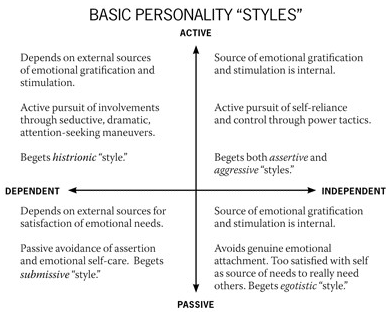
\includegraphics[scale=0.55]{Simon_character_3}
	\end{subfigure}
	\begin{subfigure}[b]{0.49\textwidth}
		\centering
		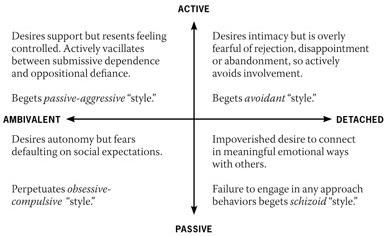
\includegraphics[scale=0.55]{Simon_character_4}
	\end{subfigure}
\end{figure}

\subsubsection{Predominately Neurotic Personalities}

\paragraph{The Deferential Pattern}
``Some predisposed individuals look externally to satisfy their emotional needs. They don't find within themselves either the resources or the confidence to tackle life's challenges, \& are overly reliant on others to provide necessary stimulation \& support. They are notoriously \textit{passive}, non-assertive, accommodating, \& acquiescent. \&, because they habitually fail to act in their own behalf, they deny themselves the opportunities for the potential successes they need to build self-confidence. They might occasionally take a chance \& venture out, but if they meet with significant obstacles or resistance, they quickly retreat \& are reluctant to try again. This then perpetuates their pattern of non-assertion.

\textit{Passive-dependent} (or simply, \textit{dependent}) is the label some clinicians \& researchers have given to those personalities. They are all too willing to concede defeat in the face of challenge, \& to turn their lives over to the care of someone else they view as more powerful, capable, \& more resilient than themselves. Because they are so emotionally dependent upon others \& lack the skill to function autonomously, they can be remarkably \textit{submissive} \& \textit{deferential} in their style of relating interpersonally.

The dependent personality is driven by several fears, namely the fears of abandonment, failure, \& even success. Failure signals to them that their self-doubts are justified, \& reinforces their perceived need of others. Success begets fears of separation from familiar sources of support. At a very deep level, these individuals equate being ``on their own'' being being ``alone,'' \& this creates intense \& deep-seated anxiety.

The dependent, interpersonal style of relating is both begotten \& maintained primarily by what these individuals do not do (hence the \textit{passive} component of passive-dependency). Typically, they don't assert themselves or act autonomously \& independently. They experience considerable anxiety w.r.t. their personal safety \& well-being, especially when they are not firmly tied to a reliable source of emotional support. Their anxieties about self-assertion \& the potential loss of support systems fuel considerable neurosis. When they say ``no,'' they too readily feel guilty. When they're tempted to challenge an oppressive situation or partner, their fears of potential abandonment kicks in. So instead of standing up for themselves \& becoming more independent, they acquiesce \& remain emotionally dependent.

The core characteristics of the Deferential Personality are:
\begin{itemize}
	\item Over-reliance on external sources of emotional gratification \& support.
	\item Excessive readiness to capitulate or submit in interpersonal encounters or when facing the challenges of daily living.
	\item A tendency to affiliate with those viewed as more powerful or capable than themselves.
	\item Apprehension, anxiety, \& other symptoms of distress when faced with potential losses of support.
\end{itemize}
There are several factors that have been advanced as possible contributors to the development of the deferential ``style'':

Possible Constitutional (biological, temperamental) Factors:
\begin{itemize}
	\item These individuals tend to have relatively pacific, retreating temperaments.
	\item They tend to have high needs for safety \& protection.
	\item They tend to be highly responsive to external reward.
\end{itemize}
Possible Learning Factors:
\begin{itemize}
	\item These individuals might have over-learned that powerful others will nurture \& protect them, possibly even better than they have learned to protect themselves.
	\item They appear to lack experience in fending for themselves emotionally, behaviorally, \& occupationally.
	\item They appear to have failed to adequately discriminate between functioning autonomously (i.e., being ``on their own'') \& being emotionally abandoned (i.e., totally ``alone'').
	\item On balance, individuals with this personality type are generally much more neurotic than they are character disturbed. If there is a dimension of their personality one could regard as character deficiency, it would be their \textit{strength} of character. These individuals are frequently seen as ``weak'' \& ineffective. They are often the archetypal ``doormats'' in relationships. They lack the necessary confidence, resoluteness, \& persistence necessary to fend for themselves, \& for others to be able to depend on them.
	\item Millon\footnote{Millon, T., \textit{Personality Disorders in Modern Life}, (Wiley, 2000), pp. 210--213.} suggests that there are some common variations of this personality type, depending upon which personality traits dominate. He proposes that the underdeveloped capacity of some dependent personalities to face life's challenges \& meet its responsibilities begets a pattern of immaturity \& inadequacy (i.e., the ``inadequate'' personality variant). The disquieted or avoidant dependent anticipates danger \& potential abandonment, unless closely aligned with trustworthy, supportive others. The overly selfless dependent cares so little about self that any sense of personal identity or worth becomes obscured or absorbed by another viewed as stronger or more powerful. The accommodating variation is overly agreeable, compliant, \& subservient, catering to the needs of others in exchange for a sense of being valued \& cared for.'' -- \cite[pp. 56--59]{Simon_character}
\end{itemize}

\paragraph{The Histrionic Pattern}
``Another personality type also depends upon external sources for satisfying emotional needs. But individuals with this personality type are very \textit{active} in pursuing those sources of support \& stimulation. They are expert at securing the involvement of others in their lives. They have a flair for the dramatic, \& a repertoire of highly seductive \& superficially appealing behaviors they employ to solicit attention \& lure others into relationships. This is the historic personality type.

Some histrionics have a marked tendency to be overly reactive \& theatrical. Heightened emotionality is part of their constitutional makeup. To some degree, however, their antics are often superficial \& manipulative. They tend to over-dramatize \& to experience the secondary gains of securing attention from others. This often leads them to form relationships that are shallow, unsubstantial, \& unstable, although they can often be quite intense.

Some histrionic personalities tend to be rather vain \& self-focused, not only seeking to be the center of attention, but becoming quite unhappy when others are not doting on them. Some are preoccupied with physical beauty \& other ``accidental'' but desirable human attributes. Others can be quite manipulative when it comes to securing the attention \& involvement they seek from others.

On balance, histrionic personalities tend to be a bit more neurotic as opposed to character-disordered. But because of some of the traits just mentioned, they are not as far toward the neurotic end of the spectrum as some of the other personalities we'll be discussing; \& certainly not as far toward that end as their passive-dependent counterparts. Vanity, superficiality, \& excessive self-focus naturally reflect poorly on anyone's character. Exactly where a particular histrionic personality lies on the character-disorder vs. neurotic continuum can vary considerably. It depends on the various other traits that might be dominant in their personality (e.g., the craving for novelty \& excitement, the tendency to be overly emotional, reactive, sensation-seeking, erratic) as well the other personality traits that might co-exist with their dominant coping style.

The core characteristics of the histrionic personality are:
\begin{itemize}
	\item Over-reliance on external sources of emotional support, gratification, \& stimulation.
	\item Active, often dramatic attempts to secure desired attention \& involvement with others.
	\item Interpersonal gregariousness.
	\item Displays of intense \& occasionally superficial emotionality.
	\item Tendency to form highly emotionally-charged but relatively shallow relationships.
\end{itemize}
Possible Constitutional Factors:
\begin{itemize}
	\item These individuals tend to crave novelty \& to be excitement-seeking.
	\item They tend to have high levels of emotionality \& reactivity.
	\item They appear highly responsive to external sources of stimulation \& reward.
\end{itemize}
Possible Learning Factors:
\begin{itemize}
	\item These personalities might have over-learned that others can be seduced or manipulated into providing attention, support, \& gratification of emotional needs.
	\item They may have failed to learned that others have value that goes deeper than the accidental attributes they possess \& the excitement or stimulation they can bring to a relationship.'' -- \cite[pp. 59--61]{Simon_character}
\end{itemize}

\paragraph{The Antisocial Pattern}
``Antisocial personalities are individuals who simply don't connect or engage with others as most of us do. What's more, they don't experience any pressing urge to do so. They have been given all sorts of clinical labels in the past such as ``schizoid'' or ``detached.'' In common parlance, they have been frequently but \textit{erroneously} labeled ``anti-social'' by individuals attempting to describe their idiosyncratic aloofness or \textit{asociality}. They are often described as ``loners'' or social isolates who don't appear to enjoy or desire the same kinds of social connection \& involvement that give most individuals' lives meaning \& richness.

Many asocial personalities appear predisposed t their style of relating as the result of biologically-based characteristics (e.g., mild autistic traits, lack of ability to respond to external stimulation \& reward, \& impoverished capacity for emotional responsiveness \& expression) as opposed to the environmental factors that often contribute to dysfunctional personality development. Some researchers suggest a dimension of human functioning \& a ``Spectrum'' of conditions exist that include schizoid personalities as well as the disorders of Asperger's Syndrome \& Autism.

Most of the difficulties these individuals experience for functioning adaptively do not appear to arise out of neurotic conflicts or deficiencies of integrity \& morality. So it's not really useful to assign them a place on the continuum of neurosis vs. character disturbance. Naturally, however, if other traits associated with either neurosis or character disturbance are also present, it can further complicate the problems such personalities experience in relating to others.

Millon\footnote{Millon, T., \textit{Personality Disorders in Modern Life}, (Wiley, 2000), pp. 315--317.} suggests some major variations of this personality, each of which is characterized by the predominance of 1 or more of their typical traits. He notes that some asocial personalities are remarkably remote \& live an almost hermit-like existence. Others appear to be extremely introversive, living in their own world, detached from others \& things around them. Some are lethargic \& energy-depressed, \& appear to have a fairly chronic anhedonia (i.e., inability to experience pleasure or joy). Others are primarily characterized by their emotional aloofness \&\texttt{/}or constriction.

The core characteristics of the Asocial Personality are:
\begin{itemize}
	\item A marked pattern of social detachment.
	\item Diminished capacity to experience pleasure in typical human social activities.
	\item Emotional constriction.
	\item Diminished capacity to react \& respond to others.
\end{itemize}
Possible Constitutional Factors:
\begin{itemize}
	\item Diminished capacity to be affected by external reward.
	\item Emotional imperturbability \& constriction.
	\item Intrinsic lethargy \& psychomotor retardation.
	\item Social detachment.
\end{itemize}
Possible Learning Factors:
\begin{itemize}
	\item It does not appear that learning failures, environmental trauma, or response to over-learning issues play significant roles in the development of this personality pattern. However, schizoid individuals generally don't experience the same types of social engagement, encouragement, reward, etc., that most of us do. So, the relative absence of such social reinforcements might play a role in the perpetuation of their interactive style.'' -- \cite[pp. 61--62]{Simon_character}
\end{itemize}

\paragraph{The Avoidant Pattern}
``Some individuals actually want to connect with others but experience inordinate apprehension about doing so. As a result, they typically ``avoid'' potential hurtful or disappointing intimate involvements. Such individuals have been often labeled ``avoidant'' personalities.

A few avoidant personalities are so hypersensitive to perceived rejection or disappointment that they misjudge the intentions \& actions of others. So they end up denying themselves reasonable opportunities for intimacy \& support. Others tend to over-react to circumstances in which they allowed themselves to be vulnerable, \& to erroneously perceive that they were mistreated, ignored, or abused. Some avoidant personalities display a marked negativity \& pessimism. Others have a characteristic but less than paranoid level of mistrust. Still others experience a fair degree of persistent apprehensiveness, especially in situations where intimate involvement with or trust of others is at stake.

Avoidant personalities will form close attachments when they perceive they've received unusual \& unquestionable re-assurance that they will not be disappointed, criticized, or rejected. Even then, however, they are likely to continually test the loyalty of those with whom they wish to bound. When they sense they are safe, they often remain involved \& loyal to the end.

Because they are so fearful of rejection or disapproval, avoidant personalities will often shy away from occupational endeavors, or other enterprises that expose them to the social spotlight, inviting the risk of being negatively evaluated. Chronically fearing to venture out, some avoidant personalities develop a marked sense of inferiority \& incompetence. By persistently not taking risks, they only perpetuate their sense of personal inadequacy.

The core aspect of their personality involves a strong desire for meaningful involvements, yet anticipation of rejection, abandonment, \& mistreatment. So avoidant personalities experience a considerable degree of chronic anxiety. Their inner turmoil about whether they can safely satisfy their basic need for affiliation begets many approach-avoidance conflicts. On balance, therefore, they are much more neurotic than they are character-disordered.

Avoidant Personalities display the following core characteristics:
\begin{itemize}
	\item Apprehensive about intimate involvements.
	\item Preoccupied with approval \& loyalty, \& hypersensitive to perceived rejection, disappointment or betrayal.
	\item Avoid intimate relationship unless given strong guarantees of acceptance, \& avoid ventures that might result in disapproval.
\end{itemize}
Possible Constitutional Factors:
\begin{itemize}
	\item Hypersensitivity to rejection\texttt{/}disapproval.
	\item Excessive anxiety, especially social anxiety.
	\item Innate shyness.
\end{itemize}
Possible Learning Factors:
\begin{itemize}
	\item Social immaturity may have led to high levels of social rejection, mockery, \& isolation.
	\item Early bonding experiences might have led to initial intimacy followed by rejection \& abandonment.
	\item Chronic avoidance of risk-taking often leads to self-perceptions of ineptness \& incapability.'' -- \cite[pp. 62--64]{Simon_character}
\end{itemize}

\paragraph{The Obsessive-Compulsive Pattern}
``These individuals are distinctively \& intensely ambivalent about 1 of the most crucial dimensions of interpersonal functioning: emotional independence vs. dependence. They want to function in an independent way, to chart their own course, \& set their own rules. But they also fear potentially losing the approval, support, \& reinforcement they desire from others. So, they keep their inner urges to rebel \& defy in close check, leading lives of conformity, \& rigid adherence to principles \& expectations. Their deep-seated ambivalence is perpetuated by what they will not let themselves do, namely from time to time cut loose \& act with relative indifference to the expectations of others.

Obsessive-Compulsives are the folks who are proverbially ``wound too tightly.'' These days, it's become fashionable once again to call them ``anal'' personalities. This gives some recognition \& credence to Freud's notion that they developed their personalities because they gained too much satisfaction, did not get sufficient satisfaction, or experienced too much trauma exercising their sphincter muscles during toilet-training, \& as a result became obsessed with ``control'' issues. The validity of this notion (especially as a general characteristic of all such personalities), however, has never been clearly demonstrated.

There are several minor variations of this personality, some whose cardinal attributes is their high level of conscientiousness. This can easily lead to work addiction, some who tend to be miserly \& no-giving, \& some who tend to be so concerned about the rules that they lack imagination \& appreciation for human emotional needs.

Obsessive-compulsive personalities are among the most neurotic of all the personality types. They suffer considerable, chronic anxiety, because underneath it all they so want to break free of their self-imposed chains, yet greatly fear to do so. They never fully mastered the developmental task outlined by Erikson of initiative vs. guilt.\footnote{Millon, T., \textit{Disorders of Personality}, (Wiley Interscience, 1981), p. 246.} Here's the main aspect of their personality that reflects negatively on their character: Their tendency to be so preoccupied with their obsessions \& compulsions that they don't fully appreciate the negative impact on others of their apparent cold \& controlling ways.

These personalities have an overly developed sense of guilt for doing things they think others will disapprove of. Overly guilt-sensitive would describe their core psychological dynamic. Their excessive desire to avoid pangs of guilt is what drives their obsessive \& compulsive behavior. They never want others to be able to convict them of wrongdoing.

Some Obsessive-Compulsives have certain other traits that make them slightly different in their overall modus operandi. Some are conscientious to a fault, harder on themselves than on anyone else, \& prone to doubting whether they can ever measure up to their own standards. Some tend to be miserly \& unforgiving \& prone to hoarding. Others tend to revel in bureaucracy \& find security in rules \& regulations. Others are overly puritanical \& dogmatic, tightly controlled morally, prudish, \& judgmental.

Obsessive-Compulsive personalities appear to be endowed with a high capacity to experience both fear \& anger. They both reduce fear \& channel anger by maintaining rigid control. Even though they are among the most neurotic personality types, some O-Cs evidence a degree of character disturbance. The thing that makes the big difference revolves around how their penchant for control is expressed. The more neurotic obsessive-compulsives cause themselves no end of grief because of the unreasonable demands they place upon themselves. Those who frequently attempt to control others \& use tactics to get others to do their bidding, in total disregard for the emotional toll it can take, have additional traits in their personality (which will be discussed later) that represent a degree of character disturbance.

The core characteristics of the Obsessive-Compulsive Personality are:
\begin{itemize}
	\item Over-conscientiousness regarding rules, propriety, etc.
	\item Perfectionism \& orderliness.
	\item Hesitance to surrender control.
	\item Rigidity \& inflexibility.
\end{itemize}
Possible Constitutional Factors:
\begin{itemize}
	\item Hypersensitivity to feelings of guilt.
	\item Excessive anxiety related to initiative vs. guilt behaviors.
	\item High limbic arousal (heightened capacity to experience both fear \& anger).
\end{itemize}
Possible Learning Factors:
\begin{itemize}
	\item Very \textit{conditionally}-approving, \& possibly overly punitive \& overly-controlling parents.
	\item Overly learned to reduce fear \& release anger through the exercise of rigid control.'' -- \cite[pp. 64--66]{Simon_character}
\end{itemize}

\paragraph{The Passive-Aggressive Pattern}
``This is an often misunderstood \& mislabeled personality type. The official psychiatric manual doesn't even recognize this as a personality pattern anymore.\footnote{\textit{Diagnostic \& Statistical Manual of Mental Disorders}, 4th Edition-Text Revision, (American Psychiatric Association, 2000), pp. 789--791.} 1 of the reasons: the confusion that's always existed w.r.t. adequately defining this personality type. In the deepest recesses of their psyches, these individuals are very bit as ambivalent as their obsessive-compulsive counterparts about whether to function in an autonomous, independent manner or to rely on others. The difference: These personalities perpetuate this ambivalence very actively in the way they conduct their interpersonal relations.

There is no escaping the ambivalence of the passive-aggressive. They might appeal to another for support, but when the support is offered they will typically reject it or stymie it. They will ask for another to take the lead, \& then resist cooperating. The label passive-aggressive was applied to these individuals early on because of the extent they displayed passive resistance to cooperation in their relationships. But over the years, the term passive-aggressive also came to be commonly, but erroneously, used by professionals \& lay persons alike to describe a very different personality type.

Life with a genuinely passive-aggressive personality is always difficult \& engenders considerable frustration. Consider the following example: A husband asks his wife where she wants to go for dinner. She replies, ``I don't know, honey, you decide.'' He says: ``Let's go to the Chinese place.'' She replies: ``Why the Chinese place? You know the last time we went there I didn't like it that much.'' He then says: ``We'll go wherever you want. Where would you like to go?'' She replies: ``I've got my hands full. You decide.'' ``Okay, let's go to Smith's Steakhouse.'' She replies: ``Now you know how that will stretch our budget, \& how that would wreck our promise to eat more healthily.'' \& on \& on it goes for the passive-aggressive personality. Equally desiring to be taken care of \& utterly resenting the idea of following someone else's lead, they actively vacillate between crying out to others for direction \& then thwarting others' attempts to take charge \& resisting the perceived demand to fall in line.

Passive-Aggressive personalities have been labeled by Millon as \textit{negativistic}\footnote{Erikson, Erik H., \textit{Childhood \& Society}, (Norton, 1950).} because of the distinctively negative character of their ongoing internal conflict, \& the whininess, poutiness, contrariness, \& infuriating uncooperativeness they display in a variety of overt as well as subtle ways. There are minor variations of this personality type, \& in each variation different aspects or traits tend to dominate. There are those whose: (1) characteristic fence-sitting \& indecisiveness are more prominent, (2) complaining \& negative mood is more pronounced, (3) negativism takes on a harsh, critical \& biting edge, \& (4) penchant for uncooperativeness is reflected in their not-so-accidental forgetfulness, dawdling, \& foot-dragging.

Unfortunately, clinicians \& lay persons alike erroneously use the term passive-aggressive when they're trying to describe deliberate (\textit{active}) but subtle, underhanded, \& otherwise \textit{covert} attempts to dominate, exploit, manipulate \& control. What's worse, there is a personality type (to be discussed later) best defined by their extraordinarily manipulative (i.e., covert-aggressive) character. Such individuals, who are not at all ambivalent about whether they want to dominate, frequently engage in crafty, hard-to-detect, ``gotcha'' behaviors \& back-stabbing. This personality type has been also erroneously labeled passive-aggressive by many. These underhanded connivers are better labeled differently, \& will be discussed at length later on. But it's important to remember that there's absolutely nothing passive about their manner of relating to others. Besides, such connivers are among the most character-disturbed of all personality types, whereas the passive-aggressive (perhaps the better descriptor would be \textit{recalcitrant}) personality is among the most neurotic.

Passive-aggressive personalities \& obsessive-compulsive personalities are similar in their deep-seated ambivalence about whether to function independently or depend upon others. They're also similar in the degree to which they are neurotic. But the ambivalence, anxiety, \& neurosis they experience have different origins. The obsessive-compulsive personality is driven by a hypersensitivity to guilt \& the desire to avoid at all costs doing something which might lead to feeling guilty. In contrast, the passive-aggressive personality is driven by an excessive sensitivity to shame. Passive-aggressives appear to have failed to master the developmental task, outlined by Erikson,\footnote{Erikson, Erik H., \textit{Childhood \& Society}, (Norton, 1950).} of autonomy vs. shame \& doubt. These individuals are overly sensitive to what appears to be a lack of unconditional approval -- not of their behavior so much -- but of themselves as persons of worth. They are deeply ambivalent about taking charge of their own lives, as opposed to relying on the approval of others. They want to act in an autonomous fashion, but they also don't want to risk the potential for self-blame should they fail. Similarly, putting themselves in a position to follow the lead of others only invites them to feel weak \& ineffectual. They are constantly in a real blind. They want others to take charge, but resent acceding to demands placed upon them. They can't seem to find the balance between doing as they wish \& relying on others. They are proverbially \& perennially caught between a rock \& a hard place.

As mentioned before, passive-aggressive personalities are, on balance, more neurotic than character disordered. However, their characteristic obstinacy, deficient capacity for autonomy, \& sometimes abrasive negativism all reflect poorly on their character.

The core characteristics of the passive-aggressive personality are:
\begin{itemize}
	\item Pervasive negativism \& complaining.
	\item Expression of anger through passive resistance (not talking, pouting, not-so-accidental ``forgetting.'')
	\item Frequent refusal to meet perceived demands of others even when self-defeating.	
\end{itemize}
Possible Constitutional Factors:
\begin{itemize}
	\item Hypersensitivity to shame. Inordinate desire for unconditional love \& acceptance.
	\item Difficulty expressing anger openly \& directly.
\end{itemize}
Possible Learning Factors:
\begin{itemize}
	\item Mixed messages about self-worth in childhood. Sometimes ``schismatic'' families in which some members are overly doting \& unconditionally regarding while others are critical, demanding, shaming, \& rejecting.
	\item Mixed messages about whether greater reinforcement comes from functioning primarily on their own vs. relying on others for direction, approval, \& support.'' -- \cite[pp. 66--69]{Simon_character}
\end{itemize}

\paragraph{The Assertive Pattern}
``Generally, this personality is fairly balanced w.r.t. the neurotic vs. character-disturbed dimension. This is an ``actively independent'' personality type. I.e., this personality actively seeks to maintain control over his\texttt{/}her life \& actively attends to getting his\texttt{/}her needs met without reliance on others. Whereas most healthy personalities have achieved an adaptive balance between the degree to which they need \& depend on others \& the degree to which they rely solely upon themselves, this personality is unabashedly self-reliant. But unlike their aggressive-personality counterparts (to be discussed a bit later), these personalities are not driven toward independence by a fierce desire to dominate or exert power over others. Rather, they simply appreciate the benefits of not depending on others. Further, in their pursuit of self-advancement, they impose limits \& boundaries upon themselves, taking care not to impinge upon or violate the rights of others. Sometimes, this is out of a neurotic sense of undue guilt or shame for doing otherwise. Sometimes the motivations are more altruistic. Most of the times, the motivation is purely pragmatic because the last thing the independent personality wants is to be at others' mercy (which they would be if caught \& sanctioned for injurious acts to others). On balance, the assertive personality is arguably among the most psychologically healthy of all personality types.'' -- \cite[p. 70]{Simon_character}

\paragraph{Predominately Character-Disordered Personalities}
``These personality types tend to lie much further toward the character-disturbed as opposed to neurotic end of the spectrum. So it's appropriate to examine them with greater depths than the other types we have discussed. Although instances occur in which their dysfunctional interpersonal ``style'' outwardly manifest underlying neurosis, for the most part these personalities are not the way they are primarily because of their unconscious fears, insecurities, \& defenses. Rather it's mostly because of their conscious yet dysfunctional \& irresponsible choices, as well as their innate predispositions about how to view the world \& interact with it. While the various character-disordered personality types have some unique characteristics, they also have some features in common. Those are:
\begin{itemize}
	\item \textbf{Problematic Attitudes \& Thinking Patterns.} Predominantly character-disturbed personalities tend to think in ways that impair healthy interpersonal relations. Sometimes, their thinking reflects deeply-rooted but erroneous \& dysfunctional beliefs about the nature of the world, their place in society, \& requirements for conducting healthy human relationships. Such erroneous core beliefs \& thinking patterns foster markedly antisocial attitudes. These in turn predispose them to engage in some of the most problematic social behaviors. At other times, the problematic ways they think reflect their persistent disdain for the truth (more about this later), their refusal to reckon honestly with themselves, \& their resistance to conform their thinking (as well as their behavior) to society's expectations.
	\item \textbf{Problematic sense of regard for self \& others.} Whether they are inordinately egocentric, harbor attitudes of entitlement, or have compete disdain for others, disturbed characters possess a distorted \& dysfunctional sense of both their own worth \& other people's value \& dignity. Because of this, their relationships tend to be shallow \& superficial at best, \& abusive \& exploitative at worst.
	\item \textbf{Disregard for the Truth.} Disturbed characters often ignore the reality of circumstances. They act in indifference to the truth about themselves \& their behaviors. Some engage in such expansive \& unbridled fantasy that truth for them is only what they imagine it to be. Others are at outright war with the truth. They know the truth, but because it might challenge their core beliefs or interfere with their various agendas, they refuse to acknowledge or accept it. Their disregard for the truth predispose the most disturbed characters to lie to themselves as well as others. To a great degree, it also predisposes them to engage in deceitful impression management (more about this later). The truth could potentially ``level the playing field'' in their relations with others, exposing character features that might give others pause. The more disordered characters so disregard truth -- with a penchant for lying so deeply ingrained \& habitual -- that they lie even when telling the truth would have no perceivable adverse consequence (i.e., the truth would do just fine).
	\item \textbf{Responsibility-Resistance Behaviors \& Manipulation Tactics.} The more character-disturbed personalities frequently engage in fairly ``automatic'' behaviors that, by their nature, obstruct internalization of pro-social values, principles, \& inner controls. These same behaviors often serve as ``tactics'' to help the disturbed character manipulate \& gain advantage over others. The tactics also reinforce the disturbed character's attempts to manage the impressions of others. We'll be exploring these responsibility-resistance behaviors \& power tactics in substantial detail.
	\item \textbf{Impression Management.} Some disturbed characters frequently engage in managing the impression others might form of them. For some, it's a matter of keeping an unrealistically inflated self-image. For others, it's more a matter of keeping others in the dark about the kind of person they're dealing with. Without exception, however, impression management primarily serves to help the disordered character maintain a position of advantage over others. If you don't really know exactly who you're dealing with, \& what their real intentions are, in their relationship with you, you're at a distinct disadvantage \& ripe for their exploitation.
	\item \textbf{Impaired Capacity for Empathy \& Contrition.} There is a big difference between regretting adverse consequences to oneself for bad behavior (e.g., getting ``caught,'' paying fines, receiving other social sanctions), \& experiencing genuine, empathy-based remorse for injury caused to others. For a person to experience any degree of genuine ``contrition,'' prompting them to change their ways, 2 things must occur: (1) they not only have to feel genuinely bad about what they have done (i.e., guilty), but (2) they must also be internally unnerved about the kind of persons they've become (i.e., shameful) through acting so irresponsibly. Their shame \& guilt can propel them to make amends to the best of their ability, to work very hard not to engage in the same misconduct again, \& to make themselves better persons. True contrition also always involves what the Greek philosophers termed ``metanoia'' or a ``change of heart.'' \& a true change of heart always involves correcting prior dysfunctional beliefs, attitudes, \& ways of doing things.
	
	Disturbed characters will often scream loudly how sorry they are; but their behavior patterns rarely reflect any genuine remorse. Sure, they can feel sorry for themselves, especially when they're caught, \& have to pay the occasional very high price for a serious misdeed. They will often protest something akin to: ``I have to live with my mistake every day,'' inviting you to pity them, view them as a victim in some way, \& imagine that they must be experiencing all sorts of inner emotional pain. Meanwhile, their tightly-held attitudes, thinking \& behavior patterns give few indications that they either appreciate or feel badly about the impact of their irresponsible conduct on others.
	
	3 real-life examples of the most disordered characters' deficient capacity for genuine empathy-based remorse remain seared into my mind. All 3 examples come from counseling sessions with sexual offenders:
	\begin{enumerate}
		\item A young man who had sexually molested his younger sister finally decided he wanted to talk about the abuse. As he began to describe in detail the things he had done to force his victim's compliance, tears began rolling down his cheeks. As a young \& naive therapist, I prepared myself for what I anticipated would be an emotional flood of regret \& remorse for the pain he had inflicted. My co-therapist (herself also crying) wanted to interrupt the session, assuming the same he was undoubtedly feeling might be ``too much'' for him to bear. But what eventually became clear was that he was feeling sorry only for himself. You see, it turned out that his tears were all about this fact: His victim had put up much less overt resistance to other (older \& physically stronger) members of her extended family who had also abused her. The resistance she put up invited him to feel like he wasn't as ``worthy'' as the others, \& this made him feel rejected \& inferior. He didn't even regret the intense brutality he used to get her to comply, but only that her ``rejection'' of him drove him to take her by such force, \& made him ``look like a bad guy.'' He admitted he was still angry with her for this.
		\item A middle-aged man convicted of participating in a brutal gang-rape sobbed uncontrollably when telling me about the crime. When talking about the source of his pain, he revealed he still believed he was the least culpable of his accomplices. He only ``went along with'' the caper whereas others had done the initial planning. He further complained that he was the last to assault his victim, barely penetrating her at the very moment police burst in on the scene, so he ```didn't even get a chance to bust a nut.'' Not only did this upset him, but he also cast himself as a ``victim'' of corrupt system: The court had ordered him to serve the same amount of time as his comrades.
		\item A white-collar rapist used date-rape drugs to facilitate his victimizations of several women. He expressed outrage at the fact that I didn't appear to believe he was sorry for what he had done. He protested that ``not a day goes by'' that he doesn't have to ``live with the consequences'' of what he did. His later enumeration of these consequences centered mostly on 3 losses: his freedom, his very profitable business, \& his stature in the community. He never expressed any appreciation for the nature of the injury he inflicted on his victims, or 1 iota of genuine sorrow for the pain he inflicted on them \& their families.
	\end{enumerate}
	Now, we can spend a lot of time examining all of the disturbingly pathological thinking at work here, but I'm trying to make 2 main points with these illustrations. 1st, not everything is as it outwardly appears. We err greatly when we assume that words of regret or even crocodile tears are necessarily prompted by genuine remorse. Some characters are so deeply disturbed that they can even feign remorse. So, when it comes to disturbed characters, you must be careful not to assume anything. \& we have to be particularly careful about traditional assumptions we've tended to make (most promoted by classical psychology paradigms) about the kind of wounded soul we've long believed must lie beneath disturbed characters. 2nd, a huge difference exists between the pain of self-pity \& genuine, empathy-based contrition. In the end, actions speak louder than words or even emotional expressions. It's so easy to say you're sorry. It's another thing to act like you're sorry \& be willing to make amends. All of us have transgressed in 1 way or another. But when people have true contrition, their greatest pain is for the injury they caused someone else; \& their actions reflect a sincere effort, not only to repair the damage, but also to change their ways. So, when people show some sign of emotion related to a terrible event, it's wrong to jump to the conclusion that they must necessarily be experiencing genuine remorse or empathy for the injury caused another. It's also important to remember that, in the case of the most severely disordered characters, the very capacity for empathy is non-existent.
	\item \textbf{Problematic temperament, mood, \& disposition.} Generally speaking, disturbed characters have abnormal \& problematic aspects of their temperament, mood, \& general disposition. These play key roles in their dysfunctional interpersonal styles. The more disordered characters possess irascible temperaments, low frustration tolerance, \& high reactivity, making them ``walking time bomb.'' Others are so emotionally labile that living with them is like riding a roller coaster of passions \& sentiments. Still others are so disagreeable that working or living with them is often an exasperating experience. But all of the most disordered characters have aspects of their temperament, mood, \& general disposition that not only contribute to the habitual ways they tend to interact, but also to the difficulty they have maintaining stable, healthy relationships.
	\item \textbf{Deficient Impulse Control.} Disturbed characters notoriously lack self-control. They act without thinking or with indifference to the potential consequences. They do things that hurt people \& (sometimes) feel bad about it afterward. They don't stop to think 1st how their actions might impact others or what consequences might occur. They have a deficient capacity to delay gratification \& lack internal ``brakes.'' Sometimes, their aggressive predispositions are so strong that they overwhelm their weak braking system \& cause a multitude of problems.
	\item \textbf{Failure to Suitably Profit From Experience.} Disturbed characters are not incapable of learning, but they frequently fail to learn what most of us hope they might from their experiences. I.e., most of us hope they would stop \& reconsider their ways of doing things, since those ways seem to invite so many problems. Instead, disturbed characters not only persist in their ways, but often solidify or even intensify them. This occurs despite ample, obvious evidence that their manner of doing things is tragically flawed.
	\item \textbf{Impaired Conscience.} Disturbed characters' consciences are not sufficiently developed to either ``push'' them to do what they should, or ``restrain'' them from doing what they shouldn't. In some of the most seriously disordered characters, conscience is virtually non-existent or absent altogether.
\end{itemize}
Although the various disturbed characters have traits in common, certain traits cluster together in some very distinct ways. This allows us to differentiate some major disturbed character types. Sometimes, the distinctions can become a little blurred when a particular disturbed character shares more than a few of the traits. But it's nonetheless helpful to categorize these personalities. So let's call attention to the primary traits they possess that cause problems in their interpersonal relations.'' -- \cite[pp. 70--77]{Simon_character}

\paragraph{The Egotistic Pattern}
``Some individuals simply cannot see themselves as anything else but the very center of the universe. Preoccupied with their own desires, concerns, \& image, their self-focus makes it difficult to give attention to or even recognize others' rights, needs, or concerns. They harbor a completely unrealistic sense of self-worth. These egotistic or narcissistic characters see themselves as inherently superior to others, \& believe they rightfully enjoy ``special'' status \& privilege. As a result, they easily come to feel \textit{entitled} to things they want \& to do whatever they wish. After all, in their minds, others \& their needs don't really count. Only they -- \& what they desire -- matters.

There are some prevailing notions about the underlying dynamics associated with this personality type. Many of these notions are not as well-founded on traditional principles as they purport to be, \& some are totally without foundation. The most popular prevailing notion: The ego-inflation that characterizes narcissism is a ``compensation'' for underlying feelings of low self-worth. This idea is generally attributed to Alfred Adler,\footnote{Adler, A., \textit{Understanding Human Nature}, (Fawcett World Library, 1954).} whose individual psychology was heavily dominated by this theory: People are in natural competition with one another for social status, \& compensate for their natural deficiencies by various mechanisms which produce ``complexes.''

I have come across a few narcissistic personalities whose apparent ego-inflation was rooted in an unresolved neurosis. For these few -- \& I do mean \textit{few} -- their displays of grandiosity \& haughtiness represented a true false self-presentation or fa\c{c}ade, masking deep feelings of inferiority \& fears of rejection. 1 theorist\footnote{Millon, T., \textit{Personality Disorders in Modern Life}, (Wiley, 2000, p. 278).} categorizes this type of individual as a narcissistic personality subtype: the \textit{compensatory} narcissist. So, neurotic narcissists do indeed exist. But \textit{the vast majority of egotistic individuals I've counseled over the years have been far more character disturbed than neurotic}. As such these individuals have displayed a sincere \& deep conviction about their superiority to others, whether or not such a belief is based on any kind of rational or solid foundation. They're not compensating for anything. They \textbf{\textit{really do think}} ``they're all that!'' Stanton Samenow has written about this\footnote{Samenow, S., \textit{Inside The Criminal Mind}, (Random House, 1984).} \& sometimes described these individuals as ``legends in their own minds.'' In fact, the shaky foundation sometimes seen for their inflated opinion of self is precisely \textit{because} they chronically overestimate their power \& worth. So, it's not that they start out with a weak foundation \& compensate for it. Rather, they spend their lives constructing the ``house'' of their self-image ``out of a deck of cards,'' unrealistically assessed regarding their strength \& integrity.

The histories of character-disturbed \& disordered narcissists are often quite different from those of neurotics, too. Sometimes they had good reason to believe they were the most powerful, important or capable persons in their immediate environment. Their mothers may have doted on them fro day 1. Their fathers may have abandoned them or abdicated all responsibility early on. Their principal caretakers might have been so inadequate that they were led to feel like the ``masters'' of their home. They may have been, in fact, the most functional \& capable person in their extended family system, with every reason to feel special or superior. If they were blessed with abundant natural gifts (e.g., physical attractiveness, technical or artistic talent, high intellectual capacity, etc.) -- \& \textit{most especially if they received much praise, adulation, \& social reinforcement from others \textbf{simply because they possessed these gifts}} -- they might have easily come by the notion that they were indeed ``special'' individuals, \& by right should have the world by the tail.

The narcissistic character is defined by the following traits:
\begin{itemize}
	\item \textbf{Inflated self-image \& sense of self-worth.} The narcissistic character sees himself as ``special'' \& more important than others. The neurotic narcissist might ``compensate'' for an impaired sense of self-worth, \& a ``fear'' of rejection for being anything less than perfect, by putting forth a false pretentiousness. But the narcissistic disturbed character genuinely believes (sometimes despite ample evidence to the contrary) that he is a most unique \& \textit{superior} creature. In 1 of the most seriously disordered character types (the psychopath), this trait is magnified to a chillingly pathological level (more about this later).
	
	The narcissistic character's self-appraisal is almost always out of whack with reality. This doesn't mean the individual's necessarily compensating for feelings of inferiority. It simply means the person's opinion of self often exceeds the situation's objective reality. Sometimes, these individuals possess very few genuine talents \& few remarkable accomplishments in their histories. Folks can be strongly tempted to erroneously presume that their inflated self-perceptions are a form of compensation. But many times they've been blessed with positives that contribute to very strong self-esteem or appraisal (e.g., talent, looks, brains, etc.). Sometimes, they've also experienced a fair degree of occupational \& vocational success. Still, it's not unusual for them to overplay \& overstate their accomplishments, \& overvalue their own worth.
	
	Sometimes professionals working with narcissistic characters -- whose histories of accomplishment are relatively lacking -- simply assume that their ego inflation must be a compensation for underlying low self-esteem. But they fail to consider this: There is a very significant differences between \textit{self-esteem} \& \textit{self-respect}. Sometimes these terms are used interchangeably. However, I find it crucial to distinguish between these very important concepts, especially because issues related to a healthy balance of self-esteem \& self-respect play pivotal roles in shaping several character types.
	
	Self-esteem literally means to estimate worth. It arises out of a person's intuitive assessment of what he has going for himself in the way of talents, abilities, etc. Self-respect, on the other hand, comes from the Latin \textit{respectere} (spectere being the root of the word spectacles) which means to look back. It arises from a retrospective assessment a person makes about what he has done with the gifts he has been given. In healthy societies, the most favorable retrospective assessments belong to those who have made meritorious efforts \& attained achievements that benefit the common good.
	
	All disturbed characters, but most especially narcissists, chronically overvalue \& claim ``ownership'' of the desirable but accidental attributes (i.e., gifts of nature or blessings of God) that foster a sense of high self-esteem. What's more, many times they get reinforcing messages from others like: ``You're so smart,'' or ``You're so talented.'' In short, they both receive \& are readily willing to claim credit for things they can't genuinely attribute to their own doing. They know what they have going for themselves, \& they equate their endowments with their identity. This inflates their egos.
	
	Narcissists \& the other disturbed characters often lack self-respect. That's because they know that, with their gifts, they haven't done enough good for others to merit a positive appraisal of social worth. In short, they lack respect because they haven't earned it. Many societies \& cultures inadequately recognize \& reward \textit{meritorious} conduct. Even some of our major religions \& philosophical schools of thought unwittingly downplay the value or even existence of human merit. Merit has to do with the manner in which a human being exercises the ultimate human power, the power to choose. Human beings are endowed with a free will. Making the meritorious choice is never easy, yet it is the essence of character. When a soldier enters a minefield knowing full well he could die, but seeks to rescue a fallen comrade, he commits a meritorious act. A father \& husband turns down a flagrant offer to engage in a tryst with an attractive co-worker. He does so out of concern for the solidity of his material commitment, the stability of his family, \& the welfare of his children. He performs an equally meritorious act. Doing the right thing is never easy. The problem: Within modern culture, \& even within major schools of religious \& philosophical belief, the value placed on such conduct is minimal. Often we expect good people to do right. Teachers \& parents rarely ``catch'' \& reward children for making the right choices, but we're quick to chastise when they choose wrongly. Jesus said: ``Render to Caesar the things that are Caesar's \& to God the things that are God's.'' If we ever want to reverse our cultural nightmare of inflated self-esteem \& deficient self-respect, we're going to have to do much better. We need to stop reinforcing people for the things which only God (or nature, if you will) can rightfully claim credit, such as their looks, their brains, their talents \& abilities; \& we must reinforce people for the truly meritorious, principled exercising of their wills, \& their willingness to subordinate their baser instincts in the service of the common good.
	
	Sometimes professionals, as well as others, are acutely aware of the disturbed character's deficiencies of self-respect. However, they often then confuse this with ``underlying feelings of low self-worth'' that they presume are being ``compensated for'' with the disturbed character's displays of grandiosity. They need to be more mindful of the distinction between self-esteem \& self-respect. A person can have too much of one \& not enough of the other. They also need to be more acutely aware of the factors that contribute to both, so they can help the person achieve a better balance. Most importantly, they need to avoid automatic presumptions about ``compensations'' that neurotic personalities engage in when they're dealing with disturbed characters.
	
	Narcissists' lack of humility w.r.t. both their natural endowments \& their success resulting from their endowments, as well as good fortune, inflates their sense of self-worth. They don't have room in their heart to acknowledge the roles of any outside factors or a higher power. They don't consider their native talents \& abilities as gifts, but rather as their defining characteristics. Humble, religious persons attribute their talents \& abilities to God or ``grace.'' Humble, non-religious persons attribute those things to a fortuitous accident of nature. The humble person also recognizes that all the raw talent in the world can't guarantee success. That, too, is dependent upon the ``grace'' of God, a certain amount of ``luck,'' opportunity, personal effort, \& working with others. Narcissists think that every blessing in their lives is the logical result of their own greatness. Even when they engage in acts of philanthropy or ``giving back'' to the community, it's generally done with a lot of fanfare. They want to further aggrandize themselves \& receive adulation. They lack the humble perspective that might foster the creed: ``To whom much is given, much is expected.''
	\item \textbf{Attitudes of entitlement.} Narcissistic characters' belief that they are \textit{entitled} to have the things they want derives from their credence that they are special \& superior individuals. Preoccupied with fantasies of unbridled success \& prestige, they believe they deserve by natural \textit{right} all the valuable things in life that most of us have to \textit{earn}. They think that, because of who they are \& their natural endowments, the world \textit{owes} them; \& they expect to be showered with recognition, adulation, \& reward. Because they believe the world owes them everything in the 1st place, they easily justify taking what they want, without feeling obligated to really pay for it through some kind of pro-social labor. They believe they have a right to anything they want simply because \textit{they} want it, \& their special nature \& status entitle them to it.
	\item \textbf{No concept of a higher power.} Narcissistic characters can't conceive of anything more important, more capable, or more potent than themselves. This leaves no room in their hearts for any concept of a higher power or authority. Now, I'm not necessarily talking about the concept of a God in a Judeo-Christian sense. As adherents to A.A. precepts know, there are many ways to conceive of a higher power. For the humanist, one needs to respect the collective ``greater good'' of society. For the non-deist scientist it might be recognizing the nature \& complexity of the physical universe that leads to humbly identifying oneself as a relatively insignificant character in a grand cosmic drama. Most of us have a deep, abiding sens that there is \textit{something} bigger than us.
	
	In the social world, most of us both recognize \& feel the need at times to pay deference to authority figures. Most of us recognize that there are people who know more than we do, possess competencies we don't, \& have been entrusted with decision-making authority over us. Narcissists have a hard time with this. They might \textit{feign} paying some deference for practical reasons, but in their heart of hearts they can't make themselves believe that anyone is in any way their superior. Lacking the humility to see themselves as inferior to anything or anyone, they don't recognize that any powers or entities exist; nor that these powers not only play a role in their success, but also place demands on them for gratitude \& a felt obligation to give back. They might give lip-service to the notion of a higher power, but they almost always leave its consideration absent from their hearts when they reflect on their lives \& their successes.
	
	As was discussed earlier, true core beliefs naturally beget certain kinds of actions. It's impossible to really believe in a higher power, subordinate your will to that power, \& then act in exploitive \& entitled ways towards others. For most of us, a belief in something that is not only greater than us, but also puts ethical demands on us, keeps us morally grounded.
	\item \textbf{Expansive fantasy.} The narcissistic character sees no reason to place limits on his abilities, or even his thoughts or desires. For him, imagining that he is something, or that he can have or do something, is akin to making it so. He finds no limits on what he can conceive or do. Similarly, he passively disregards the limitations of objective reality or truth. Reality is what the narcissistic character says it is. He is not influenced or swayed by others' judgments or opinions. The more character disturbed he is, the more he does not seek consensual validation. Rather, he finds validation in his own beliefs. As Samenow has commented, such individuals harbor the sincere belief that ``thinking makes it so.'' If they want something to be, in their mind, it is.
	
	These days, it's fairly common for some clinicians to attribute this characteristic of narcissists to a tendency toward bipolar disorder, hypomania, or mania. They then attempt to validate this view by pointing out that sometimes giving such an individual mood stabilizing medication will dampen the tendency to engage in this unrealistic thinking. However, this could also be argued: The tendency of narcissists to repeatedly engage in their unbridled fantasies \& passive disregard for objective reality might put them at increased risk for eventually developing more serious conditions such as hypomania, mania, or a bipolar disturbance.
	
	Now, I know that what I just said is likely to be quite controversial. But I don't think it's a notion that should be summarily dismissed. Ample research suggests that the link between biochemistry \& behavior is not just a 1-way street. We know, e.g., that a person who repetitively eats foods with a high glycemic index puts himself at increased risk for developing type II diabetes. We've also long known that strictly behavioral \& cognitive-behavioral treatments for obsessive-compulsive disorder result in the same types of biochemical changes in the brain's same areas as do purely medication-based treatments. Now, I'm not insinuating that t5rue Bipolar Disorder isn't a genuine condition in its own right with its own etiological factors. It can occur at times without warning in almost any personality type. What I am saying, however, is that certain personalities appear to have developed a style of relating that includes habitual ego-inflation. It's entirely possible (\& should be subjected to empirical test) that, when the pattern goes unchecked, it can eventually provide a segue into a much more serious condition.
	\item \textbf{Pathological desire for adulation \& admiration.} A narcissist can never get people to fawn over him or praise him enough. This character thrives on people being enamored with him. It's not so much that he values their opinions or that he \textit{depends} on them for a solid sense of self. Rather, he seeks to use others to fuel his massive appetite for self-aggrandizement by manipulating their attention \& praise.
	
	I had a conversation with a college classmate in which he told me of a disappointing sexual experience with a woman he had dated. Sexual conquest was a very big interest for this individual. Here was his main complaint about the particular experience he shared with me: He couldn't really enjoy himself because the woman didn't seem to be ``really getting off on'' being in bed with him. To add insult to narcissistic injury, she appeared to be merely using him to gratify herself. She was, in fact, very beautiful; but even an encounter with such an attractive person didn't really excite him. He wanted her to be enthralled with \textit{him. That} would have excited him. So, despite her stunning beauty, he couldn't perform. The frequency of his sexual exploits, the shallowness of those liaisons, \& the nature of what he was really looking for in those encounters -- these revealed just about everything one needed to know to understand his character.
	\item \textbf{\textit{Passive disregard} for the rights, needs, or concerns of others.} No one else really matters. It's all about the narcissist. It is a truly malignant egocentrism that makes it virtually impossible for the narcissistic character to develop or maintain genuine empathy. He is often completely oblivious to the emotional injury he inflicts on others. He doesn't set out to do harm, but so lacks conscientiousness about anyone else's welfare that he doesn't stop to consider the potential impact of what he says or does. The narcissist is so self-centered \& so self-absorbed, he doesn't really recognize others as independent entities with their own, wants, needs, desires, \& concerns. Sometimes he views others merely as extensions of himself. He can also view them as objects to bring him pleasure. He doesn't view them as persons of value in themselves to be respected or cherished.
\end{itemize}
The core characteristics of the Narcissistic Personality can be summarized as follows:
\begin{itemize}
	\item Unrealistic (grandiose) sense of self-worth.
	\item Preoccupation with power, brilliance, or appearance.
	\item Excessive desire for admiration.
	\item Impaired empathy \& regard for others.
	\item Excessive self-focus.
	\item Sense of entitlement.
	\item Oblivious to the wants or need of others -- exploitive.
	\item Haughtiness, arrogance toward those regarded as inferior.	
\end{itemize}
Possible Constitutional Factors:
\begin{itemize}
	\item Imperturbability. Doesn't get shaken by adverse events or challenges to perceived power \& greatness.
	\item Active imagination \& penchant for fantasy. Not constrained by the demands or confines of reality.
	\item These individuals appear to be moderately responsive to external praise but highly unresponsive to external condemnation.
\end{itemize}
Possible Learning Factors:
\begin{itemize}
	\item Received too much unconditional positive regard from others.
	\item Got too much praise for what they accidentally \textit{are} (e.g., talented, smart, physically attractive) \& not enough contingent attention or reinforcement for what they voluntarily \textit{did} to earn respect or admiration.
	\item Raised in an environment in which they were arguably the most powerful, capable, or reliable procurer of their wants \& needs.'' -- \cite[pp. 77--86]{Simon_character}
\end{itemize}

%------------------------------------------------------------------------------%

\subsection{The Aggressive Pattern}
``Some individuals are inherently warriors. They have a ``me against the world'' mentality, \& often pit themselves against others \& society's major rules \& authority structures. They don't passively disregard or place themselves above the rules like narcissists do; they actively challenge \& defy them. They have a pathological level of disgust for \textit{submissive} behavior of any kind. It riles them to think of themselves as weak or powerless, having to acquiesce or \textit{subordinate} themselves \& their wills to a higher authority. They strive to be ``on top'' \& ``in control'' (i.e., in a position of \textit{dominance}) at all times. They want to define the rules \& call the shots. They're also willing to do whatever it takes to satisfy their desires, even step all over the rights, boundaries, \& feelings of others. These are \textit{the aggressive personalities}. We'll soon be examining several subtypes of these individuals in greater detail. But before taking an in-depth look at the various aggressive personality subtypes, it will be necessary to introduce some concepts \& define some terms, especially with regard to the nature of aggression in humans.'' -- \cite[p. 87]{Simon_character}

\subsubsection{The Nature of Human Aggression}
``Aggression in human beings is not synonymous with violence. Human aggression is the forceful energy we all expend to survive, prosper, \& secure the things we want or needs. We reflect a deep-seated awareness of this fact in ur linguistics: We say things like, ``If you want something, you have to \textit{fight} for it.'' We encourage those who are sick or infirmed to rally their resources \& \textit{do battle} with their cancers, infections, other diseases. As a society, we launched a ``war on poverty.''

Humans have always done a lot of fighting. Although for years both mental health professionals \& lay persons have engaged in much denial about this most important fact, fighting is a huge part of life. It's fair to say that in the arena of human relations, when we're not making some kind of love, we're waging some kind of war (\& sometimes the distinction between the 2 activities is not all that clear). \textit{How} we fight is another matter entirely. The following diagram helps illustrate the difference between necessary, disciplined, \& potentially \textit{constructive, assertion}, \& undisciplined, \textit{destructive aggression}.'' -- \cite[pp. 87--88]{Simon_character}

\paragraph{Assertion vs. Aggression}

\begin{table}[H]
	\centering
	\begin{tabular}{|p{.48\textwidth}|p{.48\textwidth}|}
		\hline
		\textbf{Assertive Behavior} & \textbf{Aggressive Behavior} \\
		\hline
		Fair fighting (i.e., without putting the other at a disadvantage). & Seeking unfair advantage -- attempting to victimize another. \\
		\hline
		Fighting for a legitimate purpose. & Fighting for a self-serving \& possibly immoral purpose. \\
		\hline
		Fighting disciplined by self-imposed limits designed to prevent undue harm to another. & Fighting without limits or with poor limits on what you're willing to say \&\texttt{/}or do. \\
		\hline
		Always non-violent. & Sometimes violent. \\
		\hline
		Fighting constructively (i.e., with the goal of improving a situation for all concerned). & Fighting in a destructive manner (i.e., in a manner that destroys opportunities to improve a situation for all concerned). \\
		\hline
	\end{tabular}
\end{table}
There are also several major subtypes of aggression. 2 of the more important subtypes, \textit{reactive} \& \textit{predatory} (some theorists prefer \textit{instrumental}) aggression are contrasted in the next diagram.'' -- \cite[p. 88]{Simon_character}

\paragraph{Types of Aggression}

\begin{table}[H]
	\centering
	\begin{tabular}{|l|l|}
		\hline
		\textbf{Reactive} & \textbf{Predatory} \\
		\hline
		Spontaneous. & Premeditated, calculated. \\
		\hline
		Prompted by fear. & Prompted by \textit{desire} \\
		\hline
		Mostly \textit{defensive} character. &  Strictly \textit{offensive} character. \\
		\hline
		Goal is self-preservation. & Goal is \textit{victimization}. \\
		\hline
	\end{tabular}
\end{table}

\subsubsection{Reactive Aggression}
``All creatures display reactive aggression in response to a perceived threat to life or well-being. It's the kind of aggression a cat displays when it sits on the front porch \& witnesses a pit bull rounding the corner, slowly approaching, \& licking its chops. Frightened that the pit bull might be planning to make it his lunch, the cat is likely to engage in several characteristic behaviors. Its hair will stand on end. It may arch its back. It may hiss. It will brandish its claws. In a variety of ways \& in an obvious manner, it will signal its readiness to aggress. Does it want to aggress? No. Was its original intention to victimize? No. Is it primarily angry \& looking to pick a fight? No. In fact, it's primarily frightened. The last thing it wants to do is fight. Besides, it's no match for the pit bull \& would probably lose the contest. It might engage in some aggression-threatening behavior such as reaching out with its claw-displayed paws in a motion to scratch or slash. But it will only do so in response to threatening moves on the pit bull's part. All of its actions are of a strictly \textit{defense} character, \& its sincerest hope is that its potential adversary will change its mind \& move on. If the dog appears to be considering backing off, the cat will not antagonize it or otherwise provoke it into a more combative stance.

Reactive aggression is a purely \textit{spontaneous}, unplanned response to an unanticipated \& potentially serious threat to life \& well-being. It's prompted by \textit{fear}. That fear then triggers a very innate \& basic flight or fight response. The response is mostly \textit{defensive} in character, \& the purpose of any aggression-like behavior displayed is strictly to ward off or diminish the likelihood of any potential victimization.'' -- \cite[pp. 88--89]{Simon_character}

\subsubsection{Predatory (Instrumental) Aggression}
``Contrast the above scenario with that of another cat that spots a mouse in a room's corner \& fancies the rodent for lunch. It probably will not arch its back, but instead might put its belly low to the ground. Its hair does not stand on end out of fright. Instead, its hair lies normally. The cat is not terrified but both calm \& calculating. It won't hiss or make noise. \& it won't signal potential aggression by showing claws or making clawing motions. It will stead stealthily, \& as unobtrusively as possible, sneak up on the mouse \& pounce when reasonably sure of success. Its goal is not the avoidance of its own victimization but successful victimization of the mouse. It isn't praying that the mouse will react to signals \& go away. In fact, it wants the mouse to be right where it is, or in a hard-to-escape situation. Most importantly, it's not prompted to act because it's frightened. Its aggression is neither spontaneous nor based in fear, but rather carefully premeditated, prompted primarily by \textit{desire}. It's also \textit{not motivated by anger}. It's not mad at the mouse; it just wants to have it for lunch, an act that necessarily involves the mouse's destruction.

It's fairly common for mental health professionals \& lay persons alike to lack awareness about predatory aggression \& the many ways people can display it. Unfortunately, \textit{it's a common but erroneous belief that all aggression is always a defensive response to a perceived threat}. Some folks simply can't imagine why someone would aggress unless they felt threatened in some way. Other folks presume that people only aggress when they're angry. The presumption that anger is always the precipitant of aggression is the guiding philosophy behind many of the anger management programs so popular these days. Let's not go into all of the many misconceptions about aggression, \& especially the misconceptions about predatory or instrumental aggression. Instead, let's go back to the example of the cat \& the mouse. I'll ask some questions to examplify the absurdity of some of the most widely-held notions about why \& how humans aggress. Would you say that if the cat chose to eat the mouse, the cat must have felt ``threatened'' in some way? Would you say that the cat probably had ``anger issues,'' simply didn't know how to manage \& express its anger appropriately, \& ended up taking out its anger on the mouse? Would you say that the cat probably had a very traumatic history involving mice, probably in childhood, leading it to have ``trust issues'' with mice in general? That the cat anticipated maltreatment by mice, thus justifying a ``get them before they get you philosophy?'' Hopefully, by now you're having a bit of a laugh. What's not funny, however, is this: Often folks make assumptions very similar to the ones described above when trying to understand the motivations for human aggression, especially aggression of the predatory or instrumental variety.

Predatory aggression is motivated by desire. It's as simple as that. At 1 of my workshops, an attendee posed the question: ``Well, couldn't you still say that the cat was fearful that if it didn't eat the mouse it might have to go hungry? So, isn't it really still \textit{fear} after all -- the fear of not being able to satisfy this most basic need -- that motivates the cat? My reply was that one certainly \textit{could} frame things in that manner. \& such a perspective would once again reinforce the notion that fear is always the motivation for aggression. But what benefit is derived from such a perspective? Why stretch an inadequate metaphor to such an absurd degree that it finally fits when an alternative one better describes the situation's reality? Sometimes I think we get so married to our preferred ways of understanding the nature of the world around us that we simply cannot entertain a more sensible perspective. Reasonable scientists have long accepted the law of parsimony (also sometimes referred to as ``Occam's Razor''). The simplest adequate explanation of a phenomenon most often turns out to be the best explanation.'' -- \cite[pp. 89--91]{Simon_character}

\subsubsection{Other Major Types of Aggression}
``In addition to the reactive or predatory (instrumental) variety, there are some other major types of aggression:
\begin{itemize}
	\item Overt Aggression -- Open attempts to win, dominate or control.
	\item Covert Aggression -- Subtle or concealed attempts to win, dominate or control.
	\item Active Aggression -- Trying to get something you want by actively doing things \& employing tactics to victimize others.
	\item Passive Aggression -- Trying to avoid things you don't want by resisting cooperation with others.
\end{itemize}
People display \textit{overt} aggression when their bid for dominance is open \& obvious. A prize fighter in the ring attempting to knock out an opponent is displaying overt aggression. So is a corporate CEO when he openly lays out a plan to ``destroy'' the competition \& emerge as the dominant player in a particular sector of the economy. Aggression can also be \textit{covert}. I.e., a person can do his or her best to conceal any aggressive intent toward another. Keeping aggression under cover serves a dual purpose: (1) possibly being more successful in the aggressive quest (by catching the other person unaware); (2) effectively managing others' impressions \& preserving a positive image (thus keeping others from rightly discerning the aggressor's character). Besides, persons who intuitively sense the aggression, but can't objectively verify it, are quite prone to being manipulated \& controlled.

Aggression can also be \textit{active} or \textit{passive}. People \textit{actively} aggress when they \textit{do} some things deliberately to get the better of another, or to forcefully take the things they want. Conversely, they aggress \textit{passively} when they won't do things that others want them to do. Persons using the technique of a sit-down strike to protest against injustice employ passive aggression or resistance. So does a partner in a relationship when he or she won't answer, pouts, or resists cooperation with the other partner. There are still more types of aggression, several of which will become apparent as we discuss the various attributes of the aggressive personality subtypes.'' -- \cite[pp. 91--92]{Simon_character}

\subsubsection{Understanding the Aggressive Personality ``Styles''}
``As mentioned earlier, some personalities tend to view the world as a combat stage. Every situation they encounter is a contest in which they must emerge as the victor. We best describe such personalities as fundamentally \textit{aggressive} in their styles of interpersonal interaction. They are among the most disturbed in character of all the various personality types. Some aggressive characters are so wanton in their disregard for society's dictates that they frequently run afoul of the law, engage in criminal conduct, \& spend a fair portion of their lives incarcerated. These ``criminal personalities''\footnote{Yochelson, S., Samenow, S., \textit{The Criminal Personality, Vol. I: A Profile for Change}, Aronson, 1976).} have been the subject of much study over the years. They have often been given the label ``antisocial personality.'' But it's important to recognize that many other aggressive personalities exist other than the career criminal. Most of us have encountered 1 or more of these types in our daily lives. Extremely difficult to deal with, they are among the most character-disordered personalities you will ever encounter.

The various aggressive personality subtypes have many characteristics in common. They all display a pervasive style of doing battle with others \& the world at large. All the aggressive personalities also share traits common to the narcissistic personality. Some theorists tend to view the aggressive personalities as merely an aggressive variant of the narcissistic personality. What's more, 1 of the aggressive personalities is principally defined by the term \textit{malignant narcissism} (all the attributes of the narcissist carried to the most pathological extreme.) The principal distinguishing characteristic of the aggressive personalities, however, is not their narcissism. It's their penchant for aggression.

The various aggressive personality sub-types have more in common than they have differences. But there are several major aggressive personality subtypes, each defined by some fairly unique traits. Before we take a look at the major subtypes, let's outline what the aggressive personalities have in common:

All of the aggressive personalities:
\begin{itemize}
	\item \textbf{Actively seek the superior or dominant position in any relationship or interpersonal encounter.} There's a saying in the real estate business that 3 things really matter: location, location, \& $\ldots$ location. With aggressive personalities, 3 things really matter: position, position, \&, of course, position! The determination to seek this position cuts across a wide variety of situations \& circumstances.
	
	Primary interpersonal agenda for aggressive \& other character-disordered personalities:
	\begin{enumerate}
		\item Position (seek the upper hand\texttt{/}advantage\texttt{/}superior location).
		\item Position (seek to dominate, control, or win).
		\item Position (doesn't recognize or actively resists submission\texttt{/}subordination to a higher power.)
	\end{enumerate}
	Aggressive personalities strive for the dominant position at all times \& in all circumstances. This premise is very hard for the average person \& especially the neurotic individual to understand, let alone accept. It's incomprehensible for most of us to conceive that in every situation, every encounter, every engagement, the aggressive personality is predisposed to jockey with us for the superior position, even in situations with no recognizable need to do so. The failure to understand \& accept this, however, is how aggressive personalities so often succeed in their quest to gain advantage over others.
	
	More than once I've attended professional workshops in which the presenter advised that a therapist should refrain from asking probing, intimidating, or challenging questions. Why? Because that would necessarily put the client ``on the defensive'' \& prompt him to engage in acts of resistance, as opposed to allaying his ``anxieties,'' thus making it safe for him to ``open up.'' Of course, such concerns come from the notion that people simply won't fight unless they have to or feel threatened in some way. I used to observe the caveat when working with aggressive characters, until I realized it was unnecessary \& often even counterproductive. I eventually came to realize that, whether I wanted to admit it or not, aggressive personality clients had begun resisting any intervention efforts long before my 1st encounter with them. As mentioned before, neurotics troubled by their circumstances both seek \& appreciate therapeutic ``help.'' Disturbed characters are most often reluctantly pressured into the therapeutic process by an outside agent. They don't want any part of it from the beginning. They're happy with who they are \& their way of doing things. They might be superficially cordial, but make no mistake, if they're dragged into therapy, they plan from early on to fight any efforts encouraging them to change. So, the ``fight'' starts long before they 1st arrive at the office. If a therapist is not inclined to confront it directly \& set limits \& contingencies immediately, he or she is wasting the person's as well as his or her own time.
	
	My eyes were really opened to shortcomings of traditional therapeutic approaches as soon as I began confronting character-disturbed clients. 1stly, they seemed to show at least a superficial level of interest \& rudimentary respect for the challenge they knew they faced, trying to manipulate my impressions of them. 2ndly, they seemed to appreciate the cut-to-the-chase approach in which all the cards were on the table \& everything was out in the open. Lastly, I implicitly conveyed messages in my benign but firm confrontation of the issues, especially messages like: (a) ``It's my opinion that no matter what tactics you use to convince me of the contrary, you \textit{do} have a problem with your character''; (b) ``I have some techniques you can use to change the kind of person you are for the better''; \& (c) ``I'm going to waste time listening to you blame others, justify your way of doing things, or trivializing the wreck you've made of your life \& the lives of others; but I will only engage with you if you are at least to some degree willing to be open to guidance \& accepting of the need for change.'' These emerged as very powerful messages to send. Such messages led them eventually to conclude that: (1) I could not be manipulated; (2) I actually had principles (i.e., willingly subordinated myself to a higher authority) \& was willing to adhere to them; (3) I could be trusted (this is so critical because it takes away the most common excuse aggressive personalities give for their conduct). The main reason they eventually knew they could trust me is because I didn't \textit{need} them to need me or like me. I wasn't going to prostitute myself to the person or entity that referred them to me. I wasn't going to try \& manipulate these aggressive clients into tolerating me, or even eventually liking me a little through subtle seduction \& attempts to curry favor. \& I certainly wasn't going to ``frame'' their serious psychological issues in more palatable or politically correct terms to avoid confronting character concerns head-on.
	
	Many of my colleagues do not share my belief in focusing on the person himself, as opposed to solely the behaviors displayed. They think, of course, that confronting the person about his or her character instead of simply the behaviors is potentially damaging to self-esteem \& necessarily invites resistance. These critics would have a valid point if it were really true that \textit{everyone} struggles with low self-esteem like neurotics do, \& that people fight \& resist only when they feel attacked. But I have not found these assumptions to be valid. While disturbed characters' behaviors are problematic, equally if not more problematic is this sobering fact: They have chosen to define themselves as being comfortable with their negative behavior patterns, at peace with their antisocial attitudes, \& unashamed of their repeated abdications of responsibility. Not only that, but they also choose to define themselves as retaining an unwarrantedly high opinion of themselves (ego inflation) despite the big mess these patterns have created. So, who they \textit{are} -- not just what they do -- is a major issue needing attention \& confrontation. Their \textit{character} needs to be a center of focus. I also don't pretend that I'm their unconditional friend or ally. If they want my respect \& support, they'll soon learn that they earn it only by making some pretty hard choices w.r.t. changing their usual ways.
	\item \textbf{Abhorrence of submission to any entity viewed as a higher power or authority.} The aggression personalities are fundamentally at war with anything blocking unrestrained pursuit of their desires. Unfortunately, this often means society's rules, dictates, \& moral obligations, \& the expectations imposed by authority. Some aggressive personalities will accede to, or give \textit{assent} to, demands placed on them when it is expedient or self-serving to do so; but in their heart of hearts they never truly submit or subordinate themselves to a higher power or authority. It is anathema to think of themselves as under anyone else's influence, power, or control. So, they resist subordinating themselves. Their innate aversion to any kind of submissive behavior plays a critical role in their problems with forming consciences in their early development, \& profiting from experience (We'll take a closer look at this aspect of the aggressive character a bit later.)
	\item \textbf{Ruthless self-advancement, most often at others' expense.} The aggressive character is an unscrupulous competitor. He will lie, cheat, steal, ``con,'' manipulate, or do whatever he must to seek the position he wants over someone else. The end almost always justifies the means. Actively \& deliberately, aggressive personalities seek to exploit \& victimize others. Whereas the narcissist simply doesn't pay attention to others' rights or needs (because he doesn't consider them important), the aggressive character tramples their rights \& needs to satisfy his own desires. When the aggressive character wants something from you, he will take it by whatever means he finds necessary.
	\item \textbf{A pathological disdain \& disregard for truth.} Aggressive characters don't just disregard the truth, they're at war with it. Truth is the great equalizer, \& aggressive personalities always want to maintain a position of advantage. So, they deliberately play very fast \& loose with the truth when they're not flat out flying. They don't want you to ``have their number.'' That upsets the balance of power. So, they're usually about the business of conning \& duping you. \& because they want to have advantage over you, they often lie in subtle \& sophisticated ways, carefully managing your impression of them \& manipulating you through deception. Their lying is so pervasive \& automatic, they will lie even when the truth would do just fine; except lying keeps the con game going, which they perceive as maintaining the position of advantage. Also, the lying takes so many forms it's almost impossible to count them all. Nonetheless, we'll take a look at some of the major ways when we talk about manipulation tactics later on.
	\item \textbf{Defective internal ``brakes'' (lack of inhibitory controls).} Aggressive personalities are like a runaway train with no means to stop. When they're on a mission, they can't or won't put on the brakes, even when it's in the best interest of all to do so. They appear to have a constitutionally-based deficiency in their neurological inhibitory networks. But since they are also hardwired to fight so intensively \& frequently, installing such controls presents an almost insurmountable challenge during their development.
	
	When most of us are fed up with someone \& have the urge to punch their lights out, we exercise restraint, contemplating the possible negative consequences. In short, we think 1st \& act later, usually with some moderation. Because they lack inhibitory control, aggressive characters act 1st \& think or reflect later. They might even have some genuine after-the-fact regret (although the most severely disordered of these personalities lack regret or remorse); but such regret is usually too little \& too late in coming. Their lack of inhibitory control, as well as their overly aggressive predisposition, leads to their \textit{impaired ability to delay gratification}. They want what they want, \& they usually want it NOW.
	\item \textbf{Irascible Temperament.} Aggressive characters are often quick to react to any environmental event, \& their reactions are often quite intense. Someone will say something that most people would simply ignore, whereas they overreact. They have a remarkably low frustration tolerance, \& become easily upset when things don't go as they want them to go. As a result, in their development they cultivated little will to bear discomfort. It doesn't take much to set them off. They might become enraged at the slightest provocation. Say just the wrong thing, or look at them in the wrong way, \& you might find yourself facing their wrath.
	\item \textbf{Lack of Adaptive Fearfulness.} Although this characteristic is common to other disturbed characters, aggressive personalities are the most lacking in what researchers sometimes call adaptive fearfulness. They lack the squeamishness or apprehension a person should ideally have when contemplating doing something they probably shouldn't do. They neither weigh or fear the potential consequences. They frequently engage in unhealthy risk-taking, daredevil-type behavior, \& are notoriously sensation-seeking.
	
	When most folks experience a negative consequence of their behavior, they at least consider modifying that behavior. But aggressive personalities' imperturbability allows them to remain unshaken, \& therefore undeterred w.r.t. their destructive behavior patterns. In fact, adversity often prompts them to solidify their combative stance against the world. They tend to view adverse consequences as proof that the world is a cold, cruel place in which they must fight to survive. They tend to regard their tenacious facing of adversity as a noble character trait. They not only value it, but also sometimes try to intensify it with every adverse consequence they experience.'' -- \cite[pp. 93--99]{Simon_character}
\end{itemize}

\subsubsection{The World According to Aggressive Characters}
``Aggressive personalities believe every situation has only 4 possible outcomes:
\begin{enumerate}
	\item I win, you lose.
	\item You win, I lose.
	\item I win, you win.
	\item I lose, you lose.
\end{enumerate}
Naturally, they prefer the 1st possible outcome. They like it best when they win \& you lose. For them, this is the clearest indication they've emerged the victor in a contest, securing the dominant position. Contrarily, they abhor the notion that you might win \& they will lose. They resist this potential outcome with passion. It casts them in the inferior or subordinate position, which they detest. Aggressive personalities will reluctantly (although not usually graciously) accept win-win outcomes. I.e., they'll stop warning with you if they think they've secured at least some modicum of victory, even if you also end up with something you want. Tragically, if it becomes clear they're certainly headed for defeat, aggressive characters often won't go down easily. They want to take someone else with them, lessening the sting of defeat. Sadly, this scenario sometimes plays out in the tragic murder-suicides that occasionally make headlines.

To summarize, the following are the core characteristics of the aggressive personality:
\begin{itemize}
	\item Problems with authority \& societal expectations.
	\item Reckless trampling of the rights\texttt{/}needs of others.
	\item High-risk behaviors \& sensation-seeking.
	\item Problems with self-control \& delay of gratification.
	\item Frequent, sometimes flagrant, lying.
\end{itemize}
Possible Constitutional Factors:
\begin{itemize}
	\item High reactivity \& aggressive predisposition.
	\item Low anger threshold \& frustration tolerance.
	\item Deficient inhibitory capacity.
	\item Lack of adaptive fearfulness.
	\item Innate revulsion to submissive behavior modalities.
\end{itemize}
Possible Learning Factors:
\begin{itemize}
	\item \textit{Sometimes} raised in hostile, abusive, severely neglecting environments.
	\item Experienced excessive success (reinforcement) in securing goals aggressively.
	\item Insufficient experience with correctly administered punishment.
	\item Failed to learn the long-term benefits of short-term self-denial.'' -- \cite[pp. 99--100]{Simon_character}
\end{itemize}

\subsubsection{Traditional Paradigms' Failure to Accurately Understand \& Address Aggressive Personalities' Problems}
``Traditional thinking about antisocial characters has always been this: Abuse \& neglect in their histories led them to deeply mistrust the world \& others' motivations. As a result, Traditionalists thought disturbed characters found it too anxiety-evoking to ``bond'' emotionally with their primary caretakers as well as others. Within this model, aggressors' offensive postures are perceived to be an underlying \& rational ``defense'' against anticipated injury. They are seen as having adopted an ``I'll get you before you get me'' style of coping with life's challenges. Traditionalists have adhered to the notion that all human beings would naturally bond with others, behaving in pro-social ways unless severely traumatized \& conditioned to believe that others are untrustworthy. So traditional theories propose that, when they engage in their hostile acts, antisocial personalities are ``acting-out'' deeply unconscious conflicts about their safety. They perceive a cold, hostile, \& rejecting world. As a result, they reduce their internal pain \& anxiety with antisocial conduct, minimizing feelings of guilt or shame through unconscious mechanisms such as denial, projection, \& rationalization. Traditional beliefs about antisocial personalities have often been viewed as validated by the fact that such individuals frequently cast themselves as victims of mistreatment. They claim that they rightfully don't trust others, \& insist that their behavior was a matter of self-defense. Traditional perspectives have some value if, in fact, the aggressive personality is mostly neurotic. But this is actually fairly rare. The aggressive personalities are among the most frequently \& severely character-disordered individuals.

In my work over the years with disturbed characters, I have found that \textit{most} of the time, when aggressive personalities cast themselves as victims, they don't really believe they are the injured party. Rather, they want \textit{you} to believe that they think that way. They know full well that \textit{they} are the victimizers who injured others for no other reason than wanting to take something, regardless of the damage they inflicted on others. But if they can convince you that their actions weren't purely maliciously motivated, they can possibly evoke more sympathy from you, keeping you in the dark about their true character. Knowing what they're really all about would put them in a position of disadvantage with those they seek to manipulate (Remember: position, position, position!). A ``level playing field'' is something they always seek to avoid. So, they engage in deceitful games of impression management, working hard to have you see them as a victim in some way.

A few of the many aggressive personalities I've counseled over the years actually experienced significant abuse, neglect, \& trauma. But I've encountered many more who greatly exaggerated how badly they were victimized while simultaneously minimizing their history of victimizing others. I've also encountered many personalities whose childhood environments were unremarkable or as nurturing \& supportive as any -- sometimes even better than most. Yet, these individuals appear to have been ``fighters'' from the start, actively resisting the socialization process during their formative years, \& showing an inherent lack of empathy \& capacity to bond with others.

Any reasonable theory of personality formation simply has to take this into account: Countless individuals have experienced great hardship, abuse, \& trauma in their formative years; but they did not become aggressive personalities or any other type of disturbed characters. It's dangerous to make blanket assumptions about what must underlie the aggressive predispositions of these personalities. It's also dangerous to accept their stories without scrutiny, skepticism, \& objective verification. My experience with these individuals has shown me how problematic it can be to blindly accept traditional perspectives on what makes these disturbed individuals ``tick.''

In recent years, research has pointed to errors of many traditional assumptions about aggressive character formation. For many years, therapists generally accepted that ``bullies'' were in fact cowards who ``compensated'' for feelings of insecurity \& low self-esteem. They were seen as displaying bravado to mask feelings of inadequacy. They often picked on those weaker, which was regarded as ``proof'' that they inwardly felt incompetent. But some solid research has demonstrated that most bullies aren't cowards at all. They're not struggling with low self-esteem. They're merely brutes with outrageously inflated egos \& a huge sense of entitlement. We also now know that starting off as an egomaniacal brute early in life very strongly predicts all kinds of social maladjustment later in life, including possibly becoming a full-fledged antisocial personality.

Contrary to popular belief, substantial evidence shows that a history of trauma, especially abuse \& neglect, does not necessarily predispose a person toward antisocial personality characteristics. In fact, many individuals who lead antisocial lifestyles were raised in supportive \& nurturing environments. Evidence also exists that genetic factors play a significant role in whether someone will eventually display antisocial characteristics. Yet myths persist that such characters simply must have been subjected to abuse \& neglect, \& that their early trauma explains why they behave as they do.

Disturbed characters understand keenly what kinds of attitudes, beliefs, \& biases most people hold. They know full well that neurotics are quick to believe no one would engage in aggressive conduct unless they come from a disadvantaged or traumatic background. They often use this knowledge to play on others' sympathies, avoiding responsibility for their choices \& actions. But when one carefully examines their entire history \& seeks corroboration from reliable sources, here's what generally emerges: Antisocial characters (especially psychopaths) over-represent their degree of being victimized by others, \& under-represent how seriously they have intentionally \& wantonly victimized others. I usually treat their initial claims with some healthy skepticism, or possess contradictory documentation. Then such characters will often admit a much more lengthy history of doing horrible things to others. They'll also acknowledge that very few, if any, horrible things ever really happened to themselves. But I've also observed just the opposite in 2 situations: (1) when such individuals are questioned by a naive interviewer; or (2) when the disordered character senses the interviewer believes that people only do bad things because of traumas they've experienced in the past.

With all disordered characters, here's 1 very important thing to remember: Mounting evidence shows it isn't so much what bad events happened early on in their lives that shaped them. It's what \textit{didn't happen} w.r.t. the kinds of influences people need to adequately shape their characters. In some cases, the shaping influences were simply inadequate (i.e., discipline was absent, inconsistent, or improperly administered). Or the child's constitutional predispositions overwhelmed or stymied caretakers' attempts at providing \& promoting positive-shaping influences.'' -- \cite[pp. 100--104]{Simon_character}

\subsubsection{Major Aggressive Personality Subtypes}
``Both Simon\footnote{Simon, G., \textit{In Sheep's Clothing: Understanding \& Dealing with Manipulative People}, (A.J. Christopher \& Co., 1996, pp. 24--30).} \& Millon\footnote{Millon, T., \textit{Personality Disorders in Modern Life}, (Wiley, 2000, pp. 110--113).} suggest several major variations of the aggressive personality type exist. Although they share many traits in common, some important characteristics differentiate some of the aggressive personalities. As a result of my experience working with such individuals over the years, I find the patterns described below to represent the major aggressive personality subtypes:

\paragraph{Unbridled Aggressive (Antisocial) Pattern}
This aggressive personality is best distinguished by frequent, wanton violations of major societal norms \& refusal to subordinate his will in service of the greater good. When the unbridled aggressive sees something he wants, he takes it, regardless of whether his actions run afoul of the law or otherwise transgress others' rights. Unbridled aggressive personalities often have a lengthy history of criminal conduct. Many have spent a considerable amount of their lives incarcerated (repeat incarcerations are also common).

The unbridled aggressive has often traditionally been labeled the \textit{antisocial} personality. As the term implies (literally, ``against society''), this personality makes himself the adversary of the prevailing social order, engaging in a perpetual contest with others \& the world at large, seeking personal gain no matter the cost or impact on others. Some individuals use the term ``antisocial'' inappropriately to describe the social aloofness \& loner status of shy individuals, as well as the avoidant \& asocial (schizoid) personalities. But such personality types differ radically in character from the unbridled aggressive. Unbridled aggressive personalities are not afraid to engage you; they're not at all shy or lacking in the normal human urge to interact with others (although they might at times deliberately act indifferent \& aloof). Make no mistake. These folks want to engage you, but usually to get something from you, taking advantage of you, defeating you, exerting power \& dominance over you, or inflicting injury upon you.

The core characteristics of the Unbridled Aggressive Pattern are:
\begin{itemize}
	\item Brazen defiance of major social norms of conduct.
	\item Frequent engagement in behaviors that could result in social sanction if detected.
	\item Frequent brushes with the law\texttt{/}history of criminal offenses\texttt{/}convictions.
	\item History of overtly aggressive \& sometimes violent conduct toward others.
	\item Persistence in an aggressive pattern of conduct despite adverse consequences.
	\item Emboldened in the aggressive behavior pattern when they manage to ``beat the system.''
	\item Frequent parasitic lifestyle.
\end{itemize}

\paragraph{The Channeled-Aggressive Pattern}
Not all aggressive personalities are flagrant lawbreakers. 1 aggressive personality type generally refrains from allowing his overtly aggressive interpersonal style to lead to frequent \& brazen violations of the major rules. Channeled-Aggressive personalities place some limits on their obtrusive modus operandi. They generally confine their aggression to social pursuits in which others not only tolerate but often highly value the will to win at all costs. We've all encountered these tough-minded, callous, \textit{driven} people. They're determined to prosper, generally at someone else's expense. For them, all that matters is taking care of themselves. Stay out of their way, \& you might never have a problem with them. Get in their way, \& you're probably ``toast.'' Insensitivity, disregard for boundaries, extreme competitiveness, \& intolerance for weakness are their core characteristics. These personalities want to win at all costs, \& don't mind others knowing it. They display their aggressive tendencies openly \& proudly. They want all to know, see, \& respect their willingness to do whatever it takes to get what they want, \& to deal resolutely with those who would oppose them. They don't mind if others fear them or are intimidated by them. In fact, they might regard it a perverted indication of respect that they are a force with which to be contended. They are proud of their tenacity \& lack of apprehension when tackling the challenges of life. They rigidly adhere to the belief that the spoils of life's conflicts rightfully belong to those willing to fight for \& take them.

Several personality theorists have long equated aggressive personality disturbance with severe anti-sociality \& a history of criminal conduct. Indeed, the mental health community's official diagnostic manual pretty much defines the antisocial personality as a career criminal. Some researchers, however, have always recognized that only a certain sub-group of aggressive personalities can be defined by their habitual criminal lifestyles.\footnote{Millon, T., \textit{Personality Disorders in Modern Life}, (Wiley, 2000, pp. 107--108).} Channeled-aggressive personalities are very much like their antisocial (i.e., unbridled aggressive) counterparts, except they don't habitually lead lives of crime.

Channeled-aggressive personalities gravitate toward situations in which they can amass power, exert control, \& satisfy their insatiable appetites to dominate or win. They are often found in the ranks of law enforcement, military command, \& professional sports. They sometimes become heads of corporations, policy makers, administrators, \& leaders of various types. Some have the manipulative skill to favorably manage others' impressions, appearing less ruthless or even as team players. In reality, however, they are a team unto themselves, always looking out for number 1. Many times, they are respected for their ambition, drive, capability, \& tenacity.

Natural leaders, these personalities know how to get any job done. They are radically different from assertive personalities, however, because they don't pay much heed to how their actions might negatively affect others. \& they don't temper their actions to display care for others' rights, needs, boundaries, \& concerns. They are individuals who are hell to work with \& work for.

Channeled-aggressive personalities generally adhere to major social norms, but not out of a neurotic sense of guilt or shame, nor a truly altruistic regard for the greater good. A well-developed conscience is not what holds them back. Rather, it's the practical reality that they run the risk of social sanction, potentially restricting their freedom if they violate major rules. Not wanting to be hampered, they take some pains to see that nothing interferes with their quests for power \& success. They don't willingly subordinate their wills to a ``higher power'' or authority. They detest the notion that ``the man'' or ``the system'' might actually exert power over them if they've caught \& sanctioned for antisocial acts. So they do their best to avoid that possibility. But, like all aggressive personalities, they lack mature conscience \& a sense of moral obligation. So they won't hesitate to engage in minor transgressions unlikely to be discovered; or which, if discovered might result in significant social sanction. Nor will they refrain from major transgressions, including criminal behavior, when reasonably convinced (through the use of power, money, or influence) that they can get away with it.

The character deficiencies of the Channeled-Aggressive Personality become all too evident when they're convinced they won't be caught or sanctioned for breaking the rules. Believing their latest laser \& radar detectors are the best on the market, they take to the highway with reckless abandon, weave between cars, \& prove to the world they can shave at least 4 minutes off the time other hapless commuters spend getting to work. Assured that their corporate books have been ``cooked'' well enough that no oversight agency could possibly detect deception, they'll raid their company's coffers, line their pockets, \& swindle their investors. Confident they can successfully buy off corrupt officials, they'll engage in shady business deals. They're as much at odds with the rules as any other aggressive personality. \& it's not devotion to the greater good that leads them to avoid the life of the common criminal.

The principal features of the Channeled-Aggressive personality are:
\begin{itemize}
	\item Interpersonal ruthlessness \& heartlessness. Channeled-Aggressives are as disregarding of others' rights \& needs as any aggressive personality. This trait differentiates them from another actively ``independent'' type: the ``assertive'' personality.
	\item General confinement \& channeling of aggressive interpersonal conduct to non-criminal activity \& relatively socially acceptable outlets.
	\item Abdication of all controls when they're convinced they can successfully avoid detection or sanction.
\end{itemize}

\paragraph{Covert-Aggression Pattern}
Covert-Aggressive Personalities are the archetypal manipulators I 1st described in my book, \textit{In Sheep's Clothing},\footnote{Simon, G., \textit{In Sheep's Clothing: Understanding \& Dealing with Manipulative People}, (A.J. Christopher \& Co., 1996).} which, after almost 16 years in print, has been revised a 3rd time \& re-released. These personalities are not openly aggressive in their interpersonal style. In fact, they do their best to keep their aggressive intentions \& behaviors carefully cloaked. They can appear charming \& amiable on the surface, but are just as ruthless as any other aggressive personality underneath their fa\c{c}ade. They are devious, underhanded, \& subtle in the ways they abuse \& exploit others. They are power-oriented individuals who do their best to look anyway but overtly power- \& dominance-seeking. They are generally equipped with an arsenal of interpersonal maneuvers \& tactics to manipulate, exert power over, \& control others in relationships. Their tactics are generally effective because they simultaneously accomplish 2 objectives:
\begin{enumerate}
	\item The tactics effectively play on the sensitivities, vulnerabilities, \& conscientiousness of others (especially neurotic individuals). The other persons then go unconsciously on the defensive (i.e., retreating mode). This quashes all potential resistance.
	\item The tactics conceal obvious aggressive intent. The other persons have little \textit{objective} evidence that the covert-aggressive is intending to take advantage of them. Instead of trusting their ``gut'' instincts, the other persons question themselves \& get hoodwinked.
\end{enumerate}
Covert-Aggressive personalities don't proudly broadcast their combative style as do their unbridled \& channeled-aggressive counterparts. They have found that the most effective way to advance their self-serving agendas is to keep them, as well as the nature of their true characters, carefully veiled. They gain advantage over others \& catch them unaware. They've learned from experience that overtly self-serving acts are likely to invite resistance. They'd rather not have to ``fight'' openly, fairly, or constructively, because they might actually lose. So, they fight surreptitiously, hoping that by the time their victims realize they've been taken advantage of, it will be too late. They're also confident in their ability to craftily ``reframe'' the nature of events, looking good despite the damage they're doing. This makes others feel like the bad guys for doubting them, \& ``justifies'' a whole host of behaviors that negatively impact the others' lives. This manipulative skill (sometimes referred to as ``impression management'') is developed to its most pathological extreme in 1 of the other aggressive personalities, which we'll discuss later.

Also, many of the tactics covert-aggressives use are also employed by other disturbed characters. We'll present these in a later chapter.

Some covert-aggressive personalities are remarkably skilled at hiding their quests for dominance while simultaneously wielding incredible power \& influence over others. Some cult leaders, as well as masterminds of radical religious \& political movements who occasionally make headlines have this personality type. While their devoted minions might truly believe the ideology they espouse, the master-manipulators know full well that their true agenda is power only. They know all combinations of tactics to bring others under their influence.

The cardinal characteristics of the covert-aggressive personality are:
\begin{itemize}
	\item Distinctly \textit{active} yet carefully \textit{veiled} aggressive style of interpersonal relating, resulting in the abuse, exploitation, \& victimization of others.
	\item Frequent use of a variety of tactics that simultaneously conceal their aggressive intent while putting conscientious others on the defensive, thus manipulating them.
	\item Skilled at impression management. Covert-aggressives ``frame'' events to maintain a favorable image, making others doubt their own intuitive mistrust of motives.
\end{itemize}

\paragraph{The Sadistic Pattern}
Any aggressive personality is capable of causing great harm to others. However, for most of the aggressive personalities, inflicting injury or pain upon others is not their primary objective. Aggressive personalities simply want what they want \& fight tenaciously to get it. If they have to run roughshod over others to reach their goals, they will. They'll do whatever it takes to emerge victorious in an interpersonal encounter or secure the dominant or controlling position. When others either deliberately or inadvertently interfere with their quests, they attempt to remove or obliterate that interference. Sometimes their effort is violent in character, but most of the time it is simply forceful yet non-violent. They generally don't inflict any pain on others for its own sake. Rather, it's most often a secondary by-product or consequence of the overly aggressive quest to win.

Sadistic personalities differ from the other aggressive personality subtypes because inflicting pain is a primary objective of their interpersonal modus operandi. The sadist relishes hurting others, \& derives genuine pleasure (sometimes even sexual pleasure) from others' suffering \& humiliation. The sadist especially seeks to put or keep others in a degrading \& humiliating position. He wants to feel in such total control that his victims are truly helpless \& at his mercy. Sadistic personalities take the aggressive personality's quest for domination to its most pathological extreme.

Now, traditional thinking has often postulated that no one would inflict such cruelty unless they themselves had been subjected to such treatment; \& they were ``acting-out'' some sort of psychological ``payback'' against the world, or seeking a perverted sense of redress. But there's no solid, reliable, \& objective evidence for it. In fact, some studies have shown that although some highly disturbed characters \textit{report} mistreatment \& abuse in their early histories (i.e., give the ``abuse excuse'') to justify their cruel actions, such claims are often exaggerated \& sometimes bogus.

Sadistic personalities are often found in the most extreme examples of abusive relationships. Such individuals delight in physically, emotionally, \& psychologically battering \& demeaning those unfortunate souls involved with them. \&, contrary to popular belief, their victims don't usually stay with them because they are ``weak'' \& emotionally ``dependent.'' Rather, they often stay because they realize the perverted reality that they are actually safer caving into the abuser's wishes (to feel powerful \& dominant) than they might be if they were to declare their independence.

The core characteristics of the Sadistic Personality are:
\begin{itemize}
	\item Sadists actively \& intensely seek positions of dominance \& control over others.
	\item Sadists derive satisfaction (\& in some bizarre instances even experience sexual arousal) from exerting a level of control over others, leaving the victim cowering in fear, feeling helpless, utterly dependent, degraded, \& humiliated.
	\item Sadists view those perceived as weak with callousness \& disdain.
\end{itemize}

\paragraph{The Predatory Aggressive Pattern}
Among all the aggressive personalities, by far the most pathological subtype is the one I prefer to label the predatory aggressive personality. These individuals are capable of the most heinous acts. The seemingly senseless brutality they engage in sometimes makes headlines. They are the true predators among us.

This personality type has been given many different labels in the past. The term \textit{psychopathic} was 1 of the 1st labels given to this deeply disordered character. The dominant thinking at the time was that every aspect of the human personality (including antisocial characteristics) could be explained by the theory of neurosis. That theory also proposed that when neurosis became extreme, or the inner conflicts underlying it were so intense that they caused a breakdown of the more common \& sophisticated ``defenses'' that made ``normal'' neurotic functioning impossible, the result was ``psychosis.'' Cleckley\footnote{Cleckley, H., \textit{The Mask of Sanity} (4e, Mosby, 1964).} \& others conceptualized the psychopath as a personality who appeared to be sane on the surface, but whose level of sociopathic neurosis bordered on insanity. Psychopathy, therefore, was conceptualized as a nearly insane level of antisociality.

Cleckley noted that psychopaths could be superficially charming, \& appear to the casual observer as quite benign \& ordinary characters. But they could also entertain almost unthinkable beliefs \& attitudes (while not being truly delusional), \& were prone to the vilest \& seemingly senseless antisocial acts. These characteristics would lead almost anyone to question their sanity. He also incorporated into his thinking Pinnel's observations in the early 19th Century \& even some of the ancient philosophers such as Aristotle. Cleckley determined that these individuals \textit{know} their behavior would be rightfully regarded by almost anyone as irrational, yet they persist in it. This fact appeared even more irrational \&, therefore, nearly insane. But, although they know well the vileness of their behavior, psychopaths persist in it \textit{voluntarily}. So, by current definition, they are not insane. People who are \textit{psychotic} (this term is still confused by some with the term \textit{psychopathic}) are indeed sometimes capable of heinous behavior, but it is not voluntary because their brain dysfunction impairs their capacity to reason logically \& deduce right from wrong.

The term \textit{sociopath} has also been used to describe this personality type, \& has recently again come into vogue.\footnote{Stout, M., \textit{The Sociopath Next Door}, (Random House, 2006).} The psychopath label focuses more on the uniquely abnormal mental processes of this disordered personality, whereas the sociopath label focuses more on the pattern of severe social dysfunction. Over the past several decades, the terms psychopath \& sociopath have alternatively enjoyed varying degrees of popularity among clinicians \& researchers.

Some suggest that the terms psychopath \& sociopath should not be used synonymously; that each term describes a slightly different \& uniquely extreme pathological variation of the antisocial personality. In my experience, I find some merit to this notion. I have met individuals who justify their unconscionable behavior by espousing beliefs that are truly chilling but seem crazy. Although such individuals are rarely truly delusional, they appear to really hold deeply troubling beliefs \& attitudes that make them a constant danger to others. This contrasts with other equally dangerous persons who espouse beliefs that they really don't hold; but they want others to believe that they believe, thus conferring a certain degree of bizarre rationally or justification to their heinous acts. So, even though they don't believe the ``B.S.'' they sling, they \textit{say} they do. It's their way of manipulating others \& conducting their con game of impression management.

In recent times, the eminent Canadian psychologist Robert Hare has re-popularized the label of psychopathy, \& defined its characteristics with a good deal of clarity. His arduous research also helped identify the 2 principal traits (i.e., factors) that accompany this severe disturbance of character: (1) Hare indicates this is a \textit{necessary condition} for someone to be considered a psychopath. It's what others have called a viciously \textit{malignant narcissism} exemplified by the psychopath's callous, senseless, \& remorseless use \& abuse of others.\footnote{Hare, R., \textit{Without Conscience: The Disturbing World of the Psychopaths Among Us}, (Guilford Press, 1991).} Their callousness as well as their lack of capacity for remorse is, within Hare's model, due to the absence of any conscience. This results from the psychopath's non-existent capacity to bond emotionally to the human race \& to have \textit{empathy} for others. (2) This often accompanying trait is not an essential feature. It's the socially parasitic lifestyle (e.g., criminal activity, checkered work history, abusive, \& exploitive relationships) common to antisocial personalities.

The nature of the 1st factor Hare describes, \& what gives rise to it in the very disordered characters, has always intrigued me. I've strived to better understand this factor in my work over the years with individuals in the prison population. There, estimates of the percentage of persons who score highly on ``psychopathy'' rating instruments range as high as approximately 1 in 4 or 5. Such individuals are also found among the ranks of true sexual predators. I have long observed these personalities to consider themselves superior creatures in comparison to ``common'' human beings. As they see it, amoebae, plankton, \& paramecia are at the bottom of the ``food chain''; ordinary humans are higher up, to be sure; but those like themselves are definitely at the top. Viewing themselves so pathologically superior, they tend to regard every creature ``beneath'' them (in status as well as worth) as \textit{rightful} prey. So, their seriously malignant narcissism reveals an extremely pathological kind of grandiosity, as well as an extraordinary attitude of entitlement. Just as most humans don't consider it a particularly heinous act to pluck an apple off a tree \& devour it, psychopaths don't even think twice when they use, abuse, or exploit ``ordinary'' humans in whatever ways they see fit to gratify their desires. For them, \textit{ordinary} humans -- those unfortunate creatures with fears, insecurities, emotional vulnerabilities \& sensitivities, \& especially compunctions about their actions that arise from their consciences -- are innately weak, inferior, defective, \& relatively worthless beings. They're not as entitled to survival as are those like themselves, whom they regard as the \textit{fittest} of all creation. So they prey at will on those they see as beneath them, \& with great self-edifying pleasure. That's why I think the label ``predatory aggressive'' more fully \& accurately captures the pathology of these highly disordered characters.

It's natural to wonder what factors could possibly make a person become so disordered in the 1st place. \&, of course traditional frameworks have always assumed that such individuals must necessarily have been exposed to the most extreme cruelty \& neglect; that failure to bond with others \& their hostile style of relating to the world resulted from the kinds of ``defenses'' they had to mount to deal with their cold \& hostile environment. But there's no solid evidence that any of these traditional notions are valid. Ever-mounting evidence shows that the backgrounds of these individuals do no differ all that significantly from those of other personalities, including ``normal'' or relatively well-adjusted personalities. Also, there appears to be some very unique constitutionally-based differences in these individuals that predispose their unusual character development, regardless of the environments to which they've been exposed.

Some research studies have indicated that the brains of psychopaths operate differently from those of normal individuals. The differences are most striking in the brain regions that integrate our emotions with our experiences. Such findings might help explain how psychopaths are able to carry out the most heinous acts without any apparent emotion or later remorse. A constitutional predisposition to lack genuine empathy also helps explain why individuals like Scott Peterson, Ted Bundy, Bernie Madoff \& countless others have made headlines over the years. They could be so superficially charming \& normal-appearing, could come from such relatively benign backgrounds, \& yet be capable of such predatory \& heartless behavior toward others.

In my work with predatory aggressive personalities, I have encountered many who, as Hare notes, lack any modicum of conscience or empathy for others. Such individuals are truly incapable of what psychologists call ``emotional bonding'' in a relationship. They experience absolutely no remorse when they commit acts of unspeakable horror against others. But a few that I've encountered actually appear to have \textit{some} capacity for these things. Unfortunately, they also have an extraordinary capacity to mentally wall-off or ``compartmentalize'' feelings they might have -- emotions which might otherwise unnerve them or interfere with their predatory agendas. This explains, e.g., why a psychopathic child sexual predator can feel genuine hurt when his own child is injured in an accident, or bristle at the thought of sexually offending one of his own, yet be capable of the completely cold \& heartless kidnapping, brutal rape, \& murder of a child across town when he feels the need to satisfy his craving. In my experience, this capacity for compartmentalization is more disturbing. Those individuals can appear so normal much of the time that, when others get a clue about just how dangerous they might be, it's far too late.

Some people report that juts being in the presence of this kind of personality makes the hair on the back of their necks stand up. A few researchers regard this intuitive sense of danger as a ``gift'' from our ancestors, letting us know we're in the presence of a predator.\footnote{De Becker, G., \textit{The Gift of Fear: Survival Signs that Protect Us from Violence}, (Little Brown \& Co., 1997).} But not all predators give off warning ``signals,'' \& not everyone has the intuitive capacity to pick up on those signals. Some predatory aggressives appear to have an uncanny ability to charm \& manage the impressions of others, a trait that goes beyond their typical superficial glibness. Such individuals could be considered a more extreme \& predatory variation of the covert-aggressive or manipulative personality.

As a result of my work over the years with both predatory aggressives \& their victims, I have concluded the main reason these predators are so successful in manipulating others: It lies not so much in their highly effective knowledge \& use of manipulation tactics; but rather in the reluctance of normal ``neurotic'' individuals to make harsh judgments about others, or to trust their gut instincts about the kind of person they're probably dealing with. They don't attach enough significance to the ``gift of fear,'' \& mistrust their instincts. On top of it all, they're also often blinded by the notion promoted by traditional psychology theories over the years that everyone is basically good (\& most especially, just like them underneath their wall of ``defenses''). So they allow themselves to believe that a person will only behave badly when hurting, frightened, or in some kind of inner pain. Such beliefs allow them to be easily victimized by the truly heartless. By now it should be evident that entertaining traditional notions about human behavior can easily be \textit{fatal} when it comes to dealing with a psychopath.

Like all the other aggressive personalities, predatory aggressives share some characteristics of the other aggressive personality subtypes. Predatory aggressives who have significant sadistic traits are among the most notorious serial killers you've ever read or heard about. In addition to callously preying on others, they often delight in watching their victims suffer, squirm, beg for mercy, or grovel in abject humiliation. \& predatory aggressives are often noted for having incredible manipulation skills. As the most pathological variation of the aggressive personality, it's no surprise that these individuals can often have other aggressive personality traits, each of which might exist at a disturbingly pathological level of intensity.

Some researchers say that these severely disordered personalities are untreatable; that exposing them to the kinds of treatment most commonly employed actually enable them to become more skilled as predators. Why? Because in typical treatment modalities where feelings \& unconscious conflicts are still given prominence, these predators gain greater \& more intimate knowledge of others' emotional concerns \& vulnerabilities. Presently, it's rare for treatment programs or providers to actually employ models that have a genuine chance of impacting severely disordered characters. So it will be some time before reliable data emerges on whether psychopaths can, in fact, be effectively treated. The emerging new models need much more development, \& must be more widely employed before the research becomes clear.

Through my years of experience, I believe I have witnessed significant changes take place in some predatory aggressive personalities who were confined long enough, exposed to sufficient ongoing ``corrective emotional \& behavioral experience,'' \& who showed some degree of ``internalization'' of appropriate values \& standards. More work \& research need to be done. But it is becoming increasingly evident that traditional interventions are virtually useless, \& may actually make matters worse.

To summarize, the core characteristics of the predatory aggressive personality are:
\begin{itemize}
	\item Lack of empathy that severely impairs conscience formation, begetting a callous disregard \& remorseless use \& abuse of others.
	\item Persistent ``conning'' \& predatory behavior.
	\item Glibness \& capacity for charm, often superficial, but sometimes quite convincing impression management.
	\item Sometimes parasitic lifestyle.
\end{itemize}

\paragraph{The Mistrusting (Paranoid) Pattern}
Again, contrary to traditional notions, most aggressive personalities aren't motivated to take their power-oriented stance toward the world because of a deep-rooted mistrust of others, nor because they want to ``pay back'' the world for mistreatment they once suffered. Although they might claim so as a manipulation tactic, most don't really anticipate mistreatment by others nor believe the best ``defense'' is a strong ``offense.'' Rather, their offensive posture is simply a preferred way of doing things. \& often, their experience successfully rolling over others has convinced them that their strategy works. However, 1 aggressive personality ``style'' \textit{is} primarily influenced by a deep \& irrational mistrust of others.

Mistrusting Aggressive Personalities (alt. Paranoid Personalities) have a pervasive sense of wariness about others' intentions \& motivations. They are innately cynical \& vigilant, respecting others only for their perceived capacity to do harm if one's guard is dropped. They ardently strive to amass as much power as possible, concerned that others' power will inevitably be used against them. They can be extraordinarily spiteful \& vengeful; but their aggression is most often muted, subtly expressed, or carefully channeled. Fortunately, it's rarely expressed in violent ways.

Traditionalists view this ``paranoid'' personality style as deeply neurotic \& bordering on ``psychotic.'' The suspicious character of their cognitions, though not technically psychotic delusions, are most often quite irrational. On the dimension of neurosis vs. character disturbance, these individuals are equally neurotic \& character disordered. They're in part neurotic because their style of coping is truly fueled by deep inner conflicts of which they are largely unaware. But they are also very comfortable with their approach to dealing with the world. They're undeterred in their style by the adverse consequences of their typical behaviors, have distorted thinking processes \& an inflated sense of self. So they are also by definition to a great extent character-disordered.

Constitutional factors appear to play a significant role in this personality style. Their maladaptive wariness appears much less chosen as opposed to hardwired. Further, this trait appears to play a significant role in how the personality style develops in the 1st place.

The core characteristics of this personality style are:
\begin{itemize}
	\item Persistent, pervasive mistrust of others' intentions \& motivations.
	\item Absence of truly delusional (psychotic) thinking.
	\item Intensely hostile feelings, most often controlled, leading to holding grudges, unrealistic jealousy or suspiciousness, \& excessive vigilance.
\end{itemize}
Constitutional factors:
\begin{itemize}
	\item Excessive wariness, vigilance, \& suspiciousness.
	\item Tendency to interpret the nature of events, circumstances, \& others' behavior in a manner that easily ascribes malevolent, hostile intent to them.
\end{itemize}
Learning factors:
\begin{itemize}
	\item Provocative behaviors toward others invite hostile responses, thus reinforcing distorted perceptions.
	\item Hostile responses to others prompt hostile, defensive reactions from others, thus reinforcing distorted perceptions.
\end{itemize}

\paragraph{Borderline Styles}
Probably no personality pattern has been the focus of as much study \& debate as the Borderline Personality. Originally the term ``borderline'' was intended to describe personalities held together with fragile, primitive, \& ineffective ego defenses. They literally straddled the border between extreme neurosis \& outright psychosis. Indeed, some borderline personalities do experience brief but reversible psychotic episodes.

As the The Diagnostic \& Statistical Manual of Mental Disorders (DSM) notes, some clinicians tend to view the borderline style as a distinctive personality pattern (i.e., the ``unstable'' pattern). Others tend to view the phenomenon as basically representing degrees of deficiency in personality organization \& solidification. Still others assert that at heart, the borderline pattern represents a disturbance or disorder of the ``self'': The individual was never able to master the principle task of adolescence. He never developed a stable, functional identity. (Indeed 1 of the previous editions of the official diagnostic manual required that the label ``identity disorder'' be given to individuals under age 18 showing borderline characteristics unless their symptoms far exceeded the criteria for an identity disturbance.) This is compatible with the notion that the resulting instability can easily become a ``style'' of its own.

We can view the borderline personality's disturbance as a failure of varying degrees to arrive at an integrated \& stable sense of self. This helps explain the wide variety of experience people have with borderline personalities, \& how any 2 borderlines can be so very different in character. That's because all of us have a variety of different personality \textit{traits} in us. Most of us form personalities that are fairly balanced, even though some of our tendencies or traits end to be more dominant. In the case of disordered personalities, dysfunctional traits are so intensely present, unyielding, or overtly dominant that they predispose a person to problems with functioning in an adaptive manner. In the case of disturbances of character, dysfunctional traits predispose individuals to chronic problems with functioning in a socially responsible manner. In the borderline personality, part of the disturbance's nature is this: Overall personality organization is so weak that we see behavior patterns associated with many different personality styles glaringly present in the same person. So, the defining overall ``style'' of interaction for the borderline is often a multitude of shifting styles (\& some propose that, in the most extreme form, it's a multiple personality). Nonetheless, some traits tend to be more dominant than others, making for a wide degree of variability in borderline personalities. A borderline personality with prominent passive-dependent traits is a remarkably different individual from a borderline personality with prominent antisocial traits. \& a borderline personality with prominent histrionic traits is very different from one with prominent obsessive-compulsive traits, etc.

Some borderline personalities had problems successfully mastering crucial psychosocial developmental stages. They experienced so much chaos, instability, abuse, \& trauma that safe, reliable role-models were not available to them. They endured such high levels of anxiety that the all-important task of identity solidification was overwhelmingly difficult, if not impossible for them to resolve adaptively. Other borderlines seemed naturally predisposed to personality difficulty in solidifying a stable sense of self. This seems due to their inherent \& chronic instability of mood, their legendary capacity for dialectical thinking (\& therefore considerable ambivalence w.r.t. ``resolving'' any developmental conflict), \& their gross deficiencies for managing anger.

Their lack of a stable sense of self \& balanced management of various traits \& tendencies cause a pattern of instability, impulsivity, \& severely self-defeating behavior. Not knowing how to cope, \& lacking internal controls, borderline personalities are notorious for attention-seeking, reckless, \& self-damaging acts when under duress. The more dependent borderlines are inordinately clingy \& have an almost irrational fear of abandonment. The more antisocial borderlines tend to enter numerous intensely-charged but remarkably shallow, volatile, \& short-lived relationships. In some borderlines, the lack of a stable sense of self leads to a lifetime of sexual-identity confusion \& fluidity. In others, the marked tendency toward dialectical thinking creates such intense ambivalence about almost every life issue, so emotional growth \& maturation is chronically impaired. In recent years, Dialectical Behavior Therapy has demonstrated some efficacy in the treatment of this personality disturbance.

The core characteristics of the borderline personality style are:
\begin{itemize}
	\item Extreme emotional instability or lability.
	\item Intense uncertainty, instability, \& variability w.r.t. personal identity \& style of inter-relating.
	\item Intense \& contrary (dialectical) urges, impulses, thinking patterns.
	\item Erratic \& impulsive patterns of behavior including episodic acts of self-harm \& irrational displays of anger toward others.
\end{itemize}
Possible Constitutional Factors:
\begin{itemize}
	\item Deficient emotional self-regulation.
	\item Excessive tendency toward dialectical thinking.
	\item Deficient impulse control capacity.
\end{itemize}
Possible Learning Factors:
\begin{itemize}
	\item Experience of severe trauma, chaos, instability, \& chronic anxiety during formative years hampering many aspects of development.
	\item Absence of stable, reliable role models sometimes a factor impairing identity formation.
\end{itemize}
Borderlines whose dominant personality traits are more closely associated with neurosis (e.g., dependent, avoidant) tend to be more neurotic than character-disturbed. Borderlines whose dominant personality traits are more closely associated with character disturbance (e.g., narcissistic, antisocial) tend to be more character-disturbed than neurotic.

\paragraph{The Eccentric Style}
Many labels have been applied to individuals whose interpersonal style of relating is best described as ``odd'' or eccentric. These individuals appear to have such an unconventional view of the world, entertain such unusual beliefs about themselves, \& behave in such a ``weird'' or peculiar manner that they appear nearly insane. However, by definition, they are not psychotic. They do not suffer from the kind of brain dysfunction that makes rational thought impossible. They don't dysfunction is a truly ``psychotic'' manner. Their thinking is organized \& \textit{logical} in the strict sense of the word, even if it is \textit{unconventional}. They are also not plagued by hallucinations or true delusions. The term ``schizoid'' has once used to describe such individuals, but we now associate that label with the ``asocial'' or socially aloof style. In more recent times, the label ``schizotypal'' has been applied to these rare \& strangely interesting personalities.

I was once asked to interview a woman who spoke with a distinctly British accent. She carried herself in a manner that suggested she came from a long line of aristocrats. She spoke of her delight at inviting her fashionable neighbors for tea, \& was very prim \& proper in her manner. In fact, this woman was of humble origin, raised in the back woods of a southern American state. She was a perfectly delightful conversationalist \& displayed none of the cardinal signs of psychosis. She did not operate under any true delusions. Her eccentricities did not rise to the level of intensity, pervasiveness, or inflexibility to significantly impair her ability to function socially or occupationally, or cause anyone any appreciable distress. Therefore, she would not have even qualified for a diagnosis of a personality disorder. Still, she displayed many prominent traits of the schizotypal personality.

On balance, such personalities are much more neurotic than they ar character disturbed. Here's 1 of the few similarities they share with disturbed characters: They are usually quite comfortable with their style of inter-relating (i.e., their traits are ego-syntonic). However, their comfort with their personality characteristics does not fly in the face of extreme discomfort caused to others, as is the case with disturbed characters.

The core characteristics of the eccentric or schizotypal personality are:
\begin{itemize}
	\item Odd or unusual patterns of thinking, speaking, \& behavior,
	\item Impaired intimate relations except with close family members.
\end{itemize}
Possible Constitutional Factors:
\begin{itemize}
	\item Predisposed to thinking that is bizarre or seemingly irrational.
	\item Impaired ability to experience \& express normal emotions.
\end{itemize}
Possible Learning Factors:
\begin{itemize}
	\item Odd beliefs \& manner alienate others, thus reinforcing social interaction deficits.
	\item Difficulty relating normally increases anxiety which in turn fuels increased social avoidance.'' -- \cite[pp. 104--124]{Simon_character}
\end{itemize}

%------------------------------------------------------------------------------%

\subsection{The Process of Character Development}

\subsubsection{Conscience \& Character Development}
``I use catchy little rhyming saying at workshops. It sums up what must happen for values \& standards to become firmly embedded in a person's psyche. It also explains why so many disordered characters (especially the aggressive \& narcissistic personalities) don't form good consciences. They ditty goes like this: ``Internalizing a societal prohibition is at heart an act of submission.'' That's right. \textit{Internalizing} a \textit{prohibition} is most fundamentally an act of \textit{submission} to a higher power or authority. A person who truly accepts a principle of conduct, \& actively incorporates it into their conscience, willingly subordinates his or her individual will to serve the greater good. This is the very essence of healthy conscience formation.

Of all the disturbed characters, those with narcissists \&\texttt{/}or aggressive personality traits have the hardest time developing a healthy conscience. Narcissists struggle with forming good consciences because they find it difficult to even conceive of a power or cause greater than themselves. Further, their excessive sense of self-importance \& attitude of entitlement make it difficult for them to entertain the notion that anything besides what they want has any real value or importance. So, they pay little attention or heed to the wants \& needs of others.

The aggressive personalities despise the idea that anyone or anything might exert power, influence, or authority over them. They experience an innate revulsion to engaging in behaviors that even resemble acts of submission. So they wage a constant war with the potentially civilizing influences they encounter in their lives. It's not that they don't know what values \& principles others want them to adopt. They know these very well. But even though they know that society wants \& expects from them, they simply won't allow themselves to serve any master other than themselves.

Predatory aggressive (psychopathic) personalities are distinguished by their extreme lack of conscience. Their severely impaired capacity for empathy \& their extraordinary capacity to compartmentalize any sensitivity they might have make it virtually impossible for them to identify with \& care about others in the ways most of us can. Their malignant narcissism (i.e., extreme sense of superiority) prevents them from recognizing any higher power \& allows them to feel entitled to dominate \& prey upon those they view as inferior. Their deficient capacity for empathy, ability to wall-off emotion, pathological sense of superiority, \& extreme predisposition to aggressively prey all combine to make it virtually impossible to form a normal, healthy conscience.'' -- \cite[pp. 125--126]{Simon_character}

\subsubsection{Socialization is a \textit{Process}}
Let's boil down traditional schools' underlying assumptions about how people become disturbed, \& how you help them heal: People are inherently good \& geared toward health. They become unhealthy because bad or ``traumatic'' things happen to them. They develop fears \& insecurities in response to their traumas. They learn to protect themselves, cope with stress or ``defend'' themselves against emotional pain in less than optimal ways. With unconditional positive regard, empathy, \& support, they can heal their wounds, lower their defenses, overcome their fears, \& become naturally inclined once again to lead healthy, loving, compassionate lives. These principles lie at the heart of traditional psychotherapy.

Some schools of philosophical \& religious thought adopt an opposing view: Man is basically a ``fallen'' or evil creature, inherently defective. Without sufficient guidance from a higher power, \& left to his own devices, man will naturally tend to descend into all types of decadence, indecency, \& depravity. His greatest need is to be ``saved,'' especially from himself. Such views are at the heart of much religious fundamentalism.

There is also the ``nature vs. nurture'' argument. For a long time, behavioral scientists argued that we'd all be the same if we weren't subjected to very different environmental influences \& contingencies. Strict ``behaviorists'' in psychology believe that our attitudes \& actions are entirely dictated by environmental contingencies. But plenty of evidence is emerging these days showing that certain behavioral tendencies are strongly influenced by genetic, biochemical, hormonal, \& other constitutional factors.

In my work over the years with various personality types, I've encountered individuals whose early environments were so full of chaos, pain, loss, \& other trauma that they had good reason to form dysfunctional coping styles. But I have also known individuals who blossomed into unbelievably noble characters despite having endured the most horrendous upbringing \& history of trauma. I have also encountered many who, despite being reared in the most nurturing environments, having ample opportunity, \& being afforded the best of academic as well as character education, became the most disordered personalities.

So, as is almost always the case, it appears the truth about human nature lies somewhere in the middle of these various extremes. Man is neither inherently good nor evil. \& he is neither at the mercy of his genes \& biochemistry nor is he fated to behave solely as his environment has ``programmed'' him to respond. He is neither inherently defective nor saintly. \& although he's basically an animal endowed by nature with some very primitive instincts, he has the remarkable capacity to become ever so much more than a mere animal. That's what the processes of socialization \& character development are all about. Character development is a difficult, painful, complex, ongoing process.

In my book \textit{In Sheep's Clothing},\footnote{Simon, G., \textit{In Sheep's Clothing: Understanding \& Dealing with Manipulative People}, (A.J. Christopher \& Co., 1996, pp. 145-146).} I define the process of character development this way:
\begin{quotation}\it
	Character-building is the lifelong process by which we instill self-discipline \& develop the capacities to live responsibly among others, to do productive work, \& above all, to love $\ldots$ [\&] loving is not a feeling, an art, or a state of mind. It's a behavior, \& precisely the behavior to which the 2 Great Commandments exhort us to commit ourselves.
\end{quotation}
Similarly, I define a philosophy for responsible living:
\begin{quotation}\it
	Even though a person might begin life as a prisoner of the natural endowments he was given \& the circumstances under which he was raised, he cannot remain a ``victim'' of his environment forever. Eventually, every person must come to terms with him or herself. To know oneself, to fairly judge one's strengths \& weaknesses, \& to attain true mastery over one's most basic instincts \& inclinations are among life's greatest challenges. But ultimately, anyone's rise to a life of integrity \& merit can only come as the result of a full self-awakening. A person must come to know himself as well as others without deceit or denial. He must honestly face \& reckon with all aspects of his character. Only then can he freely take on the burden of disciplining himself for the sake of himself as well as for the sake of others. It is the free choice to take up this burden or ``cross'' that defines love. \& it is the willingness \& commitment of a person to carry this cross even to death that opens the door to a higher plane of existence.
\end{quotation}
None of us is born civilized. We are not naturally predisposed to be socially conscientious or responsible beings. Rather, we are inherently brutes with the capacity to develop dignity, integrity, \& communal awareness. Socialization is a \textit{process}: We transform ourselves from self-severing impulse-ridden creatures into the ``civilized,'' responsible beings we can become. This process of socialization takes many years \& an incredible amount of investment on the part of others. Other than humans, no creatures require 20 or so years of 24\texttt{/}7 education, monitoring, guidance, \& discipline to function in an adaptive, independent fashion.

Some very critical factors play key roles in developing traits that most regard as distinctive marks of a healthy \& responsible character. Biology \& temperamental factors play a role, to be sure. So do environmental circumstances \& experiences (e.g., the prevailing atmosphere in the home, \& dominant cultural values). But no matter how one is biologically predisposed, \& regardless of one's environment, certain crucial lessons must be learned at various life stages if one is to develop a balanced personality \& healthy character. What's more, individuals prone to developing certain personality styles will find it quite challenging to learn some of these lessons.

Regardless of the challenge, humans must teach these important lessons that shape character. They must be taught primarily by the most influential teachers (i.e., parents or primary caretakers), \& affirmed \& reinforced by significant others in social environment \& culture. Then it's up to the individual to take the lessons to heart, incorporating the principles of responsible living into one's character structure (i.e., to \textit{internalize} these values).

Over the years, I've come to believe in what I call the ``10 Commandments'' of sound character formation. The most fundamental principles associated with character development have been known \& debated for centuries. Socrates \& Plato mused about the various human ``virtues,'' \& religious scholars throughout the years have attempted to delineate \& codify the most essential (i.e., ``cardinal'') ones. So, there's nothing really new in the perspective I offer. But I find it helpful to incorporate time-honored principles into this framework. It lays out the most essential caveats a person must observe in learning the life lessons essential to forming good character.'' -- \cite[pp. 126--129]{Simon_character}

\subsubsection{The 10 Commandments of Character}

\begin{enumerate}
	\item \textbf{You are not the center of the universe.} Rather, you are but a small part of a greater reality more vast, complex, \& wondrous than you can even imagine. You inhabit space with many other persons, creatures, \& objects of creation. So, despite your tendency to think otherwise, it's definitely not all about you. \textbf{Be mindful of how you, your wishes, desires, \& especially your behavior impact everyone \& everything else that exists.} Conduct yourself with both caution \& concern for the consequences of your very presence on the rest of creation.
	\item \textbf{Remember, you are NOT ENTITLED to \textit{anything}.} Your very life is an \textit{unearned gift}. \textbf{Strive to be truly grateful} for the many gifts you've received. Regard life \& the miracle of creation with appropriate awe \& appreciation. Gratitude will enable you to develop a sense of obligation to value, preserve, \& promote life \& to respect all aspects of creation. Knowing how inherently indebted you really are will keep you from feeling entitled.
	\item \textbf{You are neither an insignificant speck nor are you so precious or essential to the universe that it simply cannot do without you.} Know where you fit in the grand scheme of things \& \textbf{keep a \textit{balanced} perspective on your sense of worth.} Thinking too much of yourself is as dangerous as thinking too little of yourself. Do not dismiss your accomplishments, but don't laud yourself or lord over others any position or good fortune you've managed to secure. Avoid pretense. Keeping a balanced sense of self \& being genuine will help you stay humble \& avoid false pride.
	
	Remember, you are not synonymous with your talents, abilities, or physical attributes. They are all endowments (i.e., fortunate accidents of nature, ``gifts'' of God, the universe) entrusted to you. \textbf{Recognize where things really come from \& give credit \& recognition where credit \& recognition are truly due.} Who you are \& how you are defined as a character are in large measure determined by what you do with what you've been given. The credit for your life \& innate capabilities belongs to nature or, ultimately the creative force behind nature. The credit for what you \textit{do} with all you've been given goes to you. This is the essence of \textit{merit}. Honor the life force within you as well as all who might have nurtured your potential by using your gifts for the good of all. It's not so much the outcome of your actions that matter either, for that's also not entirely in your hands. It's the effort you make that matters most. Judge yourself on your merits. Having appropriate reverence for what you've been given \& honoring the creative force through your actions is the essence of both genuine humility \& healthy self-respect.
	\item \textbf{To know, pursue, speak, \& display the truth to the best of your ability, have the utmost reverence for the truth.} Unnecessary \& brutal full disclosure is never required of you, nor is sharing every ugly thing you know to be true. But you must \textbf{be ever mindful of man's incredible capacity to deceive} himself as well as others, \& the temptation we all face to secure what we want \& avoid what we don't want through deception, cheating, \& convincing. Avoid short-cuts \& the temptation to manipulate. \textbf{Honestly \& humbly acknowledge \& reckon with your mistakes.} Always take the honest \& sincere course.
	\item \textbf{Be the master of your appetites \& dislikes.} You were meant to survive \& prosper, but you were never meant to be pampered or indulged. Your ability to experience pleasure \& pain is meant to help guide you through life, not govern your life. Taking pleasure for its own sake is almost always a pathway to destruction. Avoid greed \& excess. Be willing to endure necessary discomfort. Sometimes, one has to embrace hardship in order to grow \& love. There are 2 great drives within us all: the pleasure-seeking drive, \& the drive to thrive (i.e., to live \& prosper). We are born aligned with the pleasure principle, \& the vast majority of us remain aligned with it for most if not all of our lives. We leave the comfort of the womb in fear of life until we get our 1st taste of pleasure, \& then live in fear of death unless our pain becomes too great. But we have the power to subordinate our will to gratify ourselves to life's greater cause. No man can serve 2 masters. 1 of our 2 great drives must always be subordinate to the other. The unbridled pursuit of pleasure for its own sake (hedonism) is always the pathway to psychological ill-health \& spiritual death. Most of us need to be reborn in spirit or to remake our lives on a different operating principle. Cherishing \& advancing life (i.e., \textit{loving}) \& placing the call to love above all that might please or displease us is the surest mark of good character.
	\item \textbf{Be the master of your impulses.} Be ``mindful'' of both your inclinations \& behavior. Temper your urges with reason \& foresight. Neither rush into action nor into judgment. \textit{Think} before you act. Think not only about what you're about to do but also about the consequences. You need not be paralyzed into inaction simply by taking time to contemplate the soundless \& rightfulness of the choices you might take. \& remember, you do not have to act on every urge.
	\item \textbf{Perseverance, patience, \& endurance are not really virtues in themselves.} A man intent on robbing a large bank may spend hours or days meticulously planning \& executing his caper as well as waiting for the best time to strike. \& even some criminals remain of solid resolve in dealing with life no matter how many incarcerations or life losses they've experienced. Daring is not the same as courage or forbearance. Nor is obstinacy the same as strength of will. Still, \textbf{it is imperative that you develop solidity \& strength, as well as rightness of purpose, w.r.t. your will.} Your \textit{will} say ``yes'' or ``no'' to every temptation you face, \& that will can be strengthened with practice. But merely exercising \& strengthening will is insufficient. It's important to adhere to principles of rightful conduct. That way, when the time comes, you can ``put on the brakes'' when you're tempted to run pell-mell into trouble or ``push'' yourself to take a difficult but correct path.
	
	Willfulness in the service of justice \& righteousness is indeed a virtue. To accept moral \& social obligation, to work, \& to persevere in service of the welfare of others, to pursue justice \& live righteously (i.e., to love), are indeed the most noble ways to exercise your will. So, pledge yourself to principled living \& stay the course. Faith in something bigger than you really helps. \& faith \& commitment are the antidotes to fear.
	\item \textbf{Neither your tendency to anger nor your instinct to aggress is inherently evil, although wrath is a ``deadly sin.''} Anger is nature's way of prompting you to take action to remedy a disquieting situation. You have the right to look out for your welfare. But you also have an obligation to consider the welfare of others. Some things in life really do have to be fought for. It's important to learn when \& how to fight. When you must, \textbf{fight \textit{fairly}}. Above all, fight constructively \& for a truly just cause. Do not strive simply to win, injure, or to gain advantage over others. Expend your aggressive energy in a manner that \textit{builds} instead of destroys. Take care to respect the rights, needs, \& boundaries of those with whom you might struggle. Most especially, appreciate when it's in your best interest as well as the interest of others to back-down, back-off, concede, or capitulate. Managing your aggressive urges thoughtfully \& effectively is the task of a lifetime. Yet it is a task that, when well-done -- perhaps some than any other task you face in life -- defines your character.
	\item \textbf{Treat others with \textit{civility} \& \textbf{generosity}.} Behave responsibly \& with positive regard, even to those who do otherwise to you. While respect should rightfully be earned, treating others in the decent \& genuinely loving manner that you would want for yourself -- this is the most important of all virtues. It should be done freely \& without reservation. You don't have to condone or embrace everything someone else does to behave nobly yourself. Nor do you have to make yourself a victim by subjecting yourself to constant mistreatment. Rather, you need only remember that your character is defined not so much by how others regard you but rather how you treat them. \& it takes a strong sense of generosity \& a deep abiding faith to treat others with the kind of positive regard we wish for ourselves.
	
	Most of us are plagued with anxiety about whether we will have enough, be supported enough, be valued enough, or prosper to the degree that we would like. But we need to remember that our very existence is not an entitlement but a gift. \& despite the way it might appear at times, no one in this life has really been ``cheated'' or denied. Despite whatever hardships we might have been dealt, we have also been blessed with abundant gifts \& resources. So, we need not envy others or greedily pursue our own welfare to the detriment of others. \& from those to whom much has been given, much is expected. So, for the sake of our own well being, we must bring generosity \& free giving into all our relationships. We must treat others not necessarily as we think they deserve but with the level of care, regard, concern, \& love that we truly wish for ourselves.
	\item \textbf{To the best of your ability, \textit{have sincerity of heart \& purpose}.} Be honest with yourself about whatever you do \& the reasons you're doing it. \& be straightforward with others. Let your intentions be noble \& transparent. Harbor no hidden agendas. Avoid hypocrisy \& the tendency to cast yourself as someone or something you are not. Although you need not broadcast your every desire, sincerity is a prerequisite for developing integrity of character.
\end{enumerate}
Teaching children the 10 essential commandments of character is a difficult \& lengthy process, even in the best of circumstances. But there is little doubt in my mind that the distintegration of the archetypical, nuclear family is 1 of the main reasons for the extent of character pathology we see today. Kids do best when they have stable, committed caretakers, upon whom they can rely for support as well as direction. When parents are committed \& reliable, strong emotional bonds form between them \& their children, who are inherently ``dependent'' upon them for almost everything for many years. That bond is essential to guiding children through the inevitable power struggles \& conflicts that ensue when parents attempt to enforce discipline, rules, \& structure. Children will only subordinate their wills \& internalize principles prompted by their parents if they can truly come to believe \& trust that it's in their best interest to do so \& when they experience a healthy degree of anxiety about possibly losing the support or approval of their parents when they misbehave. When children are fortunate enough to have loving \& responsible parents, as well as siblings with whom they can experience the essential dynamics of living in a social world, most will eventually learn to be responsible.

Abusive \& neglectful families have always been capable of inflicting significant emotional scars on children. But no amount of alternative social structure \& support can match a healthy, intact family when it comes to learning all the basic social tasks like respect for authority, social give-\&-take, \& the principles of right \& wrong. Here's an ever-increasing problem for teachers in schools today: Many of their students are so under-socialized that they are completely ``unprepared'' mentally, emotionally, \& spiritually to learn. This unpreparedness is in large measure because of their impoverished home environments. One can argue that this impoverishment is material in nature. But the fact is that most economically poor homes in the western world are infinitely richer than many places in the ``3rd world,'' \& the impoverishment of which I speak is common in affluent homes as well. In the character-impoverished home, children don't get a sense of what it means for people to care for one another -- to be faithful to one another -- to sacrifice for one another -- \& to commit to rightful conduct, even under difficult circumstances. So, some schools have taken it upon themselves to teach such things as \textit{character education}. Educators then try to help a child learn what it means to be human \& responsible, as well as how to read \& write.

Coming to adhere to the 1st commandment is a difficult process. Very young children are inherently narcissistic. They're not only in their own universe; they also tend to view everything around them as extensions of themselves. Some children don't move past this primitive perspective. It can happen for a lot of reasons. Sometimes parents \& caregivers have an unhealthy \textit{need} for the children in their care. They dote on them, sending them constant messages that they are the very center of things. Sometimes a child can be so utterly disconnected from support, the only reality they know is that of their own making. In order to become a more mature, less egocentric being, every child eventually has to learn that he's a part of something greater than himself alone. All children must learn that they have an inextricable relationship to the rest of the world, \& that the nature of that relationship largely defines their character.

The 2nd commandment is also difficult to learn. We live in an age of extraordinary entitlement. We have reached a remarkable level of technological development \& material prosperity. As a result, it's easy to take almost everything we have for granted. \&, we are pretty full of ourselves for having achieved the high standard of living that many enjoy.

It's really hard to instill a sense of gratitude in our children. They grow up thinking their possessions are nothing special because most of their friends have the same things. They don't naturally have any concept of value or sacrifice. Even those without material things often grow up thinking that the rest of the world owes them. Children must be taught the value of things as well as to appreciate them.

It most western cultures, almost everything once seen as a privilege is now considered a right. The neurotics among us are largely responsible for this. In their well-intentioned desire to better the human condition, they have worked tirelessly to bring us to a point where people can \& do take almost everything good for granted. 1 of the reasons disordered characters have a characteristic sense of entitlement is because they never ``learned to earn'' the good things they want in life. They somehow came to believe that they were ``owned'' these things, \& either expected them to be handed to them or learned how to con or manipulate their way to securing them.

Children need to be taught that everything in life of any real value comes with a very real price tag in terms of human effort, endurance, \& sacrifice. Instead of growing up with expectations about what the world will give them, they need to cultivate a sense of obligation to give of themselves \& to make a meaningful contribution, thereby making the world a better place. Appreciation \& gratitude are prerequisite virtues to developing a healthy sense of moral obligation.

The 3rd commandment is crucial for character development. Almost nothing is as important as developing a right \& balanced sense of self-worth. For years, well-intentioned authors in various mental health fields wrote many articles \& books on self-esteem. They basically asserted that no one can have too much self-esteem, \& that almost all psychological problems stemmed from low self-esteem. The truth is that just as many problems develop when people think too much of themselves as when they think too little of themselves. \&, as mentioned earlier, it's ludicrous to think that people only display ego-inflation as a compensation for underlying low self-esteem. In truth, some people don't value themselves enough, whereas some value themselves entirely too much. Teaching children the balance is absolutely crucial to their character development. A parent must be a fair \& careful monitor of their child's ego development. They must be attuned to when an unsure child really needs to be built-up. They also must judge when a child has become entirely too big for his or her britches, needing a reality check \& some life lessons in humility to knock him or her down a peg or two.

There is a very dominant trend in most western cultures to lavish praise, recognition, \& even financial reward on people blessed with remarkable gifts or talents \& those who have managed to achieve great things. Yet, there's virtually no real recognition or reward given to those who display true integrity of character in their various pursuits of interactions. We give massive attention to \& heap huge financial rewards on sports figures because of their talent \& what they can do to help us satisfy our insatiable appetite for winning. But when they engage in all sorts of misconduct that reflects serious defects in their character, we are surprised. Sometimes, even when their character deficiencies become all too obvious, they are still honored, praised, or even idolized. Gone are the days when a public figure needed to display integrity of character \& serve as a positive role model in order to receive respect \& admiration of others. They also endured significant shame \& rejection from the public when they engaged in conduct unbecoming their status. We live in a culture that heaps affirmation on people for what they have been given (e.g., looks, talent, intelligence, or charm) instead of how they conduct themselves. This is a surefire way to bend an ego completely out of shape.

Parents often make the same mistake with their children. Kids need to learn what belongs to them \& what belongs to God (or a pure accident of nature, if one insists on a purely secular perspective). Kid blessed with good looks, intelligence, \& talents are used to getting frequent messages of affirmation from a wide variety of sources. What they often don't get is a lot of praise, recognition, or reward for making the tough choices in life about how to behave. In the end, they equate their value as persons with the gifts they know they possess as opposed to the caring humans they might have made of themselves. Until we recognize \& reward what matters, we'll continue to get what we've been getting: a society full of individuals with a very distorted \& unhealthy sense of self-worth.

The different varieties of religious practice have also impacted our poor understanding \& appreciation of \textit{merit}. Some faiths promote the notion that a person basically has no choice but to follow a script already laid out for them. Others preach that a person can earn paradise by behaving righteously on earth. Still others overly emphasize that the Savior's sacrifice alone opens heaven's doors for us, \& that nothing we could possibly do will earn salvation. Yet, paradoxically, advocates of this position insist that a person must engage in at least 1 act (the leap of faith acknowledgment that Christ is Savior) to be personally rescued. Even the 1st apostles debated the role \& importance of meritorious conduct. Paul, of course, claimed that faith in Christ is the singular vehicle of salvation. James \& Peter insisted that one cannot say they ``believe'' without corresponding action. It seems they had a very early understanding of the intimate \& inextricable connection between one's thinking \& core beliefs \& one's actions, as well as the principle that actions speak much louder than words. It's easy to ``profess'' with one's lips a belief in a person or principle. It's quite another to demonstrate with one's actions that faith truly abides in one's heart. Jesus himself spoke of this when citing the false righteousness \& hypocrisy of the elders \& scholars in his religion.

Not only do talents \& abilities belong to ``God,'' but so do outcomes \& circumstances. Although we can frequently \& safely predict likely outcomes of our actions, this leads us to falsely believe we are in control of outcomes. In fact, we only have power over our actions. True, most often there will be predictable results. But there are no guarantees. Sometimes, despite our best \& most conscientious efforts, we do not realize anticipated or desired outcomes. Ultimately, the results of our actions are in the hands of God (late, if you will). Thinking that we're solely responsible for what happens can lead us to despair if things don't go well or to overconfidence \& ego-inflation if things turn out just as we planned. Whenever we leave our ``higher power'' out of the equation, we run the risk of getting our egos bent out of shape.

The 4th commandment addresses 1 of the difficult challenges facing individuals as they try to develop good character: It's always been easier to cheat, lie, \& steal than to take the honest path. Judeo-Christian tradition prohibits bearing false witness (intentional misrepresentation to injure someone else). Theologians differ as to whether this commandment also forbids other forms of lying. In my experience working with disturbed characters, \textit{all} the lying they do is damaging, including the lies they tell to themselves.

Human beings have an incredible capacity to deceive. Traditionally-oriented theorists have frequently advanced the notion that people desire to avoid feelings of shame \& guilt, which lies at the heart of why they lie. But I have witnessed people who lie for a vast number of reasons other than merely avoiding pangs of guilt or shame.

For the most part, lying is simply \textit{easier} than accepting \& dealing with the truth. It's a quick way to prevent something we don't want, or to secure something we want but might require more than we're prepared to give.

We live in a world full of lies \& liars. Companies will promote a food product as ``thicker \& richer'' when what they've really done is add more filler, cut costs, \& improved profits. News programs \& political pundits put various ``spins'' on the day's events or actions of others to advance their agendas \& hide their biases. Being honest is a difficult task almost any time, but being honest with ourselves is especially hard. Reckoning with our shortcomings, the reality of our circumstances, \& striving to better ourselves is very hard work. We are not creatures naturally attracted to the idea of work. \& some personalities have a virulent aversion to work.

Jesus reportedly said that the truth shall make a person free because, ultimately, the very personification of evil \& slavery to sin is the lie. In the book of Malachi there is a saying that ``truth is mightier than all things.'' In my work with disturbed characters, I have found incredible power in the truth. It's the basis of trust \& ultimately of the genuine human connection that facilitates positive change. Some therapists make the mistake of placing their own desire to be liked \& to appear affirming above everything else. I think the truth must take precedence. Now, delivering the truth in a manner that is truly \textit{benign} (i.e., loving), is an incredible challenge \& a genuine art. It requires that the therapist be simultaneously accepting, of pure intention, \& genuinely (i.e., ``brutally'') honest without being brutal at all. I have worked with many young persons struggling with character development issues who shared a smile, gave a wink, nodded in acceptance, or verbalized the greatest appreciation for being unreservedly confronted about their issues. They instinctively trust \& respond to those who tell the unvarnished truth, but who their gut tells them mean no harm.

Truth not only sets us free \& enables us to trust, but also carries with it a significant burden. Truth forces us to acknowledge our frailty. It then challenges us to reckon with that frailty \& rise above it. The truth is rarely pretty, but it is almost always redemptive \& transformative.

Parents trying to instill good consciences in their children can follow the same basic guidelines: honesty \& truth, not to produce shame \& guilt, but to develop an understanding of reality. Shame \& guilt are powerful instruments of shaping behavior, but some children don't respond to shame or guilt very well, \& some don't respond to shaming or guilting at all. Children (\& adults) are better off when confronted with truth that is both ``inescapable'' \& non-distortable, so they don't develop a pattern of self-deception. Children are much more likely to acquiesce \& acknowledge the truth when confronted about their behavior in a frank but totally benign manner, devoid of denigration or condemnation.

The 5th commandments flies straight in the face of the values promoted by our age of greed \& sensual license. We are a society of gluttons, sex ``addicts,'' \& coveters of various sorts. We want to indulge every craving we have, \& we are forever raising the thresholds of satiation. Here's what it has gotten us: a glut of Wall Street swindlers, behavioral addicts of all persuasions, \& a populace out of control physically, emotionally, psychologically, \& spiritually. At the heart of these problems is a failure to subordinate the pleasure-seeking principle upon which most of us have operated since birth. From a psychological perspective, if there's any way a person of character needs to be ``born again'' it's w.r.t the most fundamental governing principle upon which we operate. Folks who don't transcend or subordinate the pleasure principle are doomed to be enslaved by it, causing many problems for themselves \& society.

The 6th commandments goes to the heart of cognitive-behavioral techniques for helping people change patterns that impair their character development. For the most part, disturbed characters act 1st \& think later. This pattern starts early in their development. Constitutional predispositions affect this, too. As mentioned before, some personalities appear to have a constitutionally-based lack of adaptive fearfulness. \& when a person lacks apprehension about what he's about to do, he's less likely to engage in any meaningful contemplation before he acts. For a variety of reasons, some influenced by constitution, some arising out of learned experience, the actions of disturbed characters are often not tempered by sound advance reasoning.

When raising kids, we want them not only to think before they act, but to think rightly \& with due respect for the principles of moral conduct. Inevitably, doing the wrong thing is the easier path. What we want them to do, however, is to display the strength of will \& character to make the harder, more responsible choice. The mistake most parents make is that children make right decisions all the time \& barely get noticed for it. It's important to build up a high potential for right-acting by routinely reinforcing the little things they do correctly. Then kids will have sufficient strength \& soundness of will to face greater temptations as they come along.

The 7th commandment addresses the development of strength of purpose \& will. I owe a profound debt of gratitude to a very early pioneer in cognitive-behavioral therapy, Abraham Low. These days, some of his techniques might be regarded as antiquated, even evoking laughter from mental health professionals. But Low founded a program to help individuals who had suffered from what used to be called ``nervous breakdowns'' (i.e., intense levels of anxiety, depression, \& other syndromes causing a person's usual coping ability to collapse). Such persons were often hospitalized. Because very few medications existed for them at that time, they had to learn techniques to manage their symptoms. These included any ``residual'' symptoms such as anxiety or depression, once they were able to leave the hospital. His program focused on the thinking patterns of individuals, as well as the behaviors they engaged in that perpetuated their problems. So, he was pioneer in the realm of cognitive-behavioral therapy (without really knowing it). He wrote a few books \& put out some audiotapes of lectures that participants in a self-help group called ``Recovery, Inc.'' used to change their lives \& prevent ``relapses.'' 1 of his lectures was entitled ``The Will Says `Yes' or `No.''' This concept literally saved my life. By practicing the principles it advocated, I discovered that the human will, like any other natural endowment, can be \textit{developed \& strengthened} through appropriate exercise. Wow! What a concept! There are ways for a person to strengthen the will! \& to top it off, it's the will that determines whether or not we do something we're tempted to do (i.e., the will says ``yes'' or ``no'' to an urge). Within a matter of months, I was transformed from a person almost enslaved by my needs, desires, urges, \& fears to a person who could direct the course of his own life through the exercise of his will. I will forever be grateful.

Will-training is a fundamental job of parenting. Appropriate development of will is crucial to delaying gratification, persisting on difficult tasks, enduring hardships, \& having the courage to meet \& overcome challenges. As parents, we want our children to have strength of will, but we also want to shape \& temper their willfulness without breaking their spirit. Some naturally willful children must learn to bend more, \& some naturally passive children must learn to assert themselves more. In the end, how the will is shaped greatly affects the kind of character that will form.

The 8th commandment involves learning to manage our anger \& aggressive impulses. Although not all aggression is rooted in anger, there is a relationship between anger \& aggression. Everyone must learn to moderate both the emotion of anger as well as temper their urge to aggress. This is how a solid character forms.

Generally speaking, anger is an adaptive emotion that prompts us to take action to remove a threat to life or well-being. Anger that is chronic or excessive has been linked to a host of problems, including heart disease. So the emotion does need to be regulated. We also need to learn when our anger is righteous versus when it serves no purpose or has gotten out of control. I am not of the belief that kids should be allowed to throw their temper tantrums until they ``run out of gas.'' Such a tact only reinforces the notion in the child that it's okay to pitch a protracted snit; it pulls no limits on emotional expression. Nor do I believe that every outburst should be stifled precipitously, leading the child to believe he has no right to protest; that only builds resentment. A healthy balance must be struck here.

When it comes to aggression, the stakes could not be higher. People naturally do a tremendous amount of fighting in life. Humans are the only creatures to do so much of their fighting against \& among themselves. Children have to learn why, when, \& how to fight, as well as why, when, \& how to back down, concede, or acquiesce. Perhaps no lessons are as crucial to character development as these.

Among the most disturbed characters, the aggressive personalities are notoriously undisciplined \& unscrupulous fighters. From early in their development, individuals with aggressive personality traits appear to have been overly ready to lash out, significantly lacking in ``internal brakes.'' For that reason, their aggressive behavior usually needs to be confronted early on in their cycles of escalation. This gives them a fair chance at developing the mechanisms of self-control they so desperately need.

The 9th commandment embraces true charity. The world is often misunderstood. It comes from a Greek word ``caritas,'' which describes a particular type of loving behavior: an abiding respect for \& kindness toward other human beings. It is not synonymous with giving aid to the poor, which has become 1 of its most popular meanings. Rather, it is basic regard for the value of human life, which can inspire acts of almsgiving (merely giving to the poor need not be rooted in genuine \textit{caritas}) as well as other acts of human kindness. Charity requires empathy, which is why individuals with an impaired capacity for empathy (i.e., psychopaths) find  this behavior so foreign.

St. Paul put charity in the spotlight in 1 of his most famous letters to Christian converts living in ancient Corinth, extolling it even over the other timeless virtues of faith \& hope. He also pointed out how empty a life can be without it. Perhaps there is no command more constructive in the development of character than the call to ``do everything with love (caritas).''

Teaching children to love in this way is relatively simple (i.e., straightforward) yet as difficult as any parental task can be. That's because parents are required to model this behavior fairly consistently through example, large \& small. Parents need to remember to do everything -- from setting limits \& expectations to saying ``no'' \& withdrawing support -- not with resentment for the ordeal, but with love.

The 10th commandment, teaching sincerity of heart \& purpose, is a difficult task, also. If 1 is not surrounded by others of solid character (often the case), sincerity receives a poor welcome. So it's easy to learn how to present a false face. Neurotics hide their true feelings \& intentions for fear of rejection. Disturbed characters sometimes hide their true selves \& their real agendas for more nefarious purposes. The sincere course, however, is most often the best course, if not in the short run, then in the long run. Our entire social environment would take on a marvelous, productive character if more of us were willing to risk sincerity, \& to engage in honest, open communication \& debate. Many of our most pressing social problems have lingered far longer than necessary because of our impaired ability to have an honest, open, sincere discussion \& debate on the issues.'' -- \cite[pp. 129--146]{Simon_character}

%------------------------------------------------------------------------------%

\subsection{Thinking Patterns \& Attitudes Predisposing Character Disturbance}
``Here's 1 of the central tenets of the cognitive-behavioral paradigm: An inextricable relationship exists between a person's core beliefs, the attitudes those beliefs engender, the patterns of thinking various beliefs \& attitudes predispose, \& the ways the person will tend to behave as a result of his thinking. E.g., a husband may believe that women are naturally inferior to men \& should therefore be subservient. Then he might tend to think his wife is ``getting way too big for her britches'' whenever she asserts her point of view or tries to stand up for herself. He may engage in all sorts of problematic actions in an effort to ``keep her in her place.'' How we think greatly influences how we act. The major premise of cognitive-behaviorally-oriented therapy is that we can change the way we think -- \& when we do, it will necessarily impact the way we behave.

Disturbed characters don't act the way most people do largely because they generally don't think the way others do. They often don't hold the same values, harbor the same attitudes, share the same core beliefs, as most folks. Their way of thinking is marked by a ``distorted'' view of reality \& an impoverished sense of accountability.

How disturbed characters think is always reflected in the ways they act. Their ways of thinking can also be discerned from the things they say, but to a much lesser extent. That's because the things they say don't necessarily reflect beliefs they hold with genuine conviction. This is a very important fact to remember.

For some time, most clinicians \& researchers using the cognitive-behavioral model have known that the ``cognitive distortions'' of disordered characters can represent \textit{actual} but \textit{erroneous} beliefs. Sometimes, they have developed these beliefs with total obliviousness to the ways that most other people think about things. But my experience has taught me that disturbed characters can also entertain their twisted views with full awareness of how most people might think about the same situation. I'm also struck by how often the research literature will categorize the types of thinking errors disturbed characters engage in based simply on the things they frequently say. This is problematic because what they say does not necessarily reveal how they really think. Sometimes they say things to make other people believe that they think a certain way, as a manipulation technique. In reality, their \textit{behavior} is a much more reliable indicator of their true thoughts \& attitudes. So, corrective treatment programs largely based on ``challenging'' strictly verbally espoused beliefs, \& then ``teaching'' alternative ways of thinking, are not likely to be successful.

In my work with disturbed characters, I have found that some disordered characters were truly raised in environments so impoverished in multiple dimensions that their beliefs about the nature of the world, \& how to operate within it, understandably became quite skewed. So, they developed patterns of thinking \& attitudes that most responsible people don't share. Ask such people what they were thinking when they engaged in some troublesome behavior, \& what they tell you is actually what they believe, as irrational as it might sound. But with many disordered characters, the things they tell you, as well as the things they tell themselves, are nothing more than part of an elaborate ``con game.'' Such folks are very aware of how most people tend to think, \& how out of step their purported way of thinking is. But they tenaciously protest their contrary point of view to justify themselves \& their actions. They try to manipulate others into the notion that their behavior had some rational basis other than the simple intent to victimize. Sometimes, after lying so often they might even succeed in duping themselves about the distorted perspectives they advance; but they will often back off their ridiculous contentions when firmly challenged. E.g., a repeat wife beater might very well know how society at large feels about abusive spouses' violence toward women. Nonetheless, he might try to justify his behavior by constantly complaining that his wife is a vindictive ``bitch'' who constantly eggs him on. So she rightfully ``had it coming'' when she finally heaped more ``disrespect'' on him than anyone could possibly stand. This type of offender might very well know how most people would look at his situation. \& he probably also knows full well who the victimizer is \& who is the real victim. Nevertheless, such a person might do all he could to convince another to adopt the point of view that he was a victim of sorts \& therefore ``justified'' in his actions; not so much because he needs or wants validation, but because if he can get you to buy into at least part of his argument, he succeeds in casting himself in a slightly more favorable light. You might then see him as an ignorant \& perhaps misguided soul who simply ``doesn't get'' how to view women; he needs only to learn better. He's not really a person who already ``gets it'' just fine yet vehemently resists adopting the standards he knows society wants him to accept. In reality, he doesn't want to be correctly pegged by others for the dangerous person such an attitude makes him.

I can't overstate the importance of being skeptical about what disordered characters say. Remember, a great deal of the time they're engaged in a game of manipulation \& impression management. Early in my work, I interviewed several child molesters who tried to advance the notion that their inappropriate touching of their victim was not motivated by aberrant sexual desire; rather it was a foolish or misguided attempt to ``teach'' the child about sexual behavior. I asked myself, ``Do they really believe what they're saying?'' The treatment manuals I had read seemed to regard this type of thinking as a truly held belief, needing correction by ``illuminating'' the offender. Adopting this perspective, the goal of treatment became to educate him about the damage caused the child \& help him overcome the ``denial'' he was experiencing about other motives, such as his deviant urges. But I eventually learned that \textit{most} of the time, child molesters that said such things didn't really believe what they were saying. They hoped that I would believe they did, so that I would neither ascribe the appropriate degree of malevolence nor the correct motivation (e.g., sexual interest in a child) to their behavior. If I bought their excuse, I might, e.g., see them as an undereducated, poorly guided soul who make a stupid mistake, instead of as a predatory pedophile or a heartless psychopath. So, the thinking they reflected with their talk was not truly a belief. More importantly, their misrepresentations weren't based in ``denial,'' shame, or guilt. In fact, genuine guilt or shame would likely have kept them from offending in the 1st place. Rather, the ``twisted'' justification they were providing was merely an attempt to manipulate \& impression-manage others.

A child molester enrolled in a required treatment program readily volunteered to me that he knew his thinking process was ``twisted.'' He told me that prior to treatment, he had the erroneous belief that his actions were actually okay. Incestuous behavior, he said, was so common throughout his extended family that he truly believed it was ``normal.'' This made some rational sense. But being the skeptic I've learned to be, I did some digging. I learned that not only was such behavior not ``normal'' in his family, but, because of the outrage \& suspicion of family members, he'd gone to great \& elaborate lengths to keep his actions under the radar. After I confronted him, he reluctantly reported that he knew very well that it ``sounded better'' to cast himself as the product of an abnormal environment who simply didn't know better. Once again, his actions (the things he did to guard against discovery) were the more reliable indicator of his true thinking.'' -- \cite[pp. 147--150]{Simon_character}

\subsubsection{Some Major Thinking Errors}
``Stanton Samenow\footnote{Samenow, S., {\it Inside The Criminal Mind}, (Random House, 1984).} was among the early researchers to catalogue the more common distorted thinking patterns or \textit{errors in thinking} that some of the most severely disturbed characters display. Over the years, I've adapted \& modified several of these problematic thinking patterns, adding some of my own that I believe played a crucial role in relationship problems of disordered characters I have treated. In the various character-disturbed personalities, some thinking errors are more common than others \& some tend to cluster with others. The major problematic thinking patterns are:

\paragraph{Egocentric Thinking}
The disturbed character is almost always concerned with \& for himself. Whatever the situation, it's always about \textit{him}. He frequently finds himself thinking about things that \textit{he} wants, because that's what's important to him. He hardly ever thinks about what someone else might want or need, because he attaches so little importance to that. Because he thinks the entire world revolves around him, he believes it's the duty of others to place what he desires or what interests him above everything else.

When he wants something, the disordered character also doesn't consider whether it's right, good, legal, or if his pursuit of it might adversely affect anyone; he only cares that he wants it. His constant concern for himself \& the things he desires promotes an \textbf{\textit{attitude of indifference}} to the rights, needs, wants, or expectations of others. Such an attitude fosters a complete \textbf{\textit{disregard for social obligation}}. In some cases, as Samenow notes, there's an ardent distain for \& total \textbf{\textit{refusal to accept obligation}}. As self-centered as he is, the disturbed character believes the world owes him everything \& that he owes the world nothing. Such thinking is the reason the disturbed character develops an attitude of entitlement. He has extremely high expectations for everyone else, but feels no sense that he should submit himself to the expectations of others or society in general. His egocentric thinking patterns, attitudes, \& their resultant behaviors prompt him to lead an extremely \textit{self-centered lifestyle}.

\paragraph{Possessive Thinking}
Disturbed characters tend to view their relationships as possessions that they rightfully \textit{own}; they should be able to do as they wish with these people. This type of thinking frequently accompanies \textbf{Heartless Thinking}: The disturbed character tends to \textit{objectify} others (i.e., view them as mere \textit{objects} or pawns to manipulate as opposed to individuals of worth with whom one has to form a co-equal relationship). Possessive \& heartless thinking promote a \textit{dehumanizing attitude}. This makes it more likely that the disturbed character will view others, not as human beings, but as objects of pleasure, vehicles to get things he wants, or simply potential obstacles in his path that must be removed.

Possessive \& heartless thinking make it all but impossible for the disturbed character to view others as individuals with rights, needs, boundaries, or desires of their own, \& beings of dignity worthy of respect \& consideration. Such thinking is carried to a most pathological extreme in the Predatory Aggressive or ``Psychopathic'' personality.

\paragraph{Extreme (All-or-None) Thinking}
Disturbed characters frequently see things in terms of black \& white, all-or-none. They might take the position that, if they can't have all that they ask for, they won't accept anything. If someone doesn't agree with everything they say, they will frame it as not being valued or listened to at all. If they don't see themselves completely on top \& in total control, they will cast themselves as being on the bottom \& under someone else's thumb. This erroneous way of thinking makes it virtually impossible for them to develop a reasonable sense of give \& take in their relationships. It promotes an \textit{uncompromising attitude} that impairs their ability to develop any sense of moderation in their behavior patterns.

\paragraph{Inattentive Thinking}
Some researchers describe this thinking error as the ``mental filter''\footnote{Samenow, S., {\it Inside The Criminal Mind}, (Random House, 1984).} because disturbed characters selectively ``filter'' what goes on around them, paying attention to \& heeding only the things they want to, \& disregarding all the rest. They hear what they want to hear, remember what they want to remember, \& learn what they want to learn. They invest themselves intensely in the things that interest them; but they actively disregard the things they don't care about, even though they may be quite aware that others want them to pay more attention to these things. They use the responsibility-avoidance tactic of \textit{selective attention} (discussed later): They ``tune out'' someone who's trying to teach them a lesson, or only half-listen whenever they hear something they don't like. They do this most often when others are urging them to submit themselves to pro-social values \& standards of conduct. So this erroneous way of thinking is a major reason they develop both \textit{lackadaisical antisocial attitudes}. In turn, their devil-may-care \& antisocial attitudes predispose them to chronic \& unyielding behaviors that conflict with major social norms.

\paragraph{Deceptive (Wishful) Thinking}
Disturbed characters are prone to seeing things as they want instead of as they really are. 2 of their core characteristics -- the ease with which they lie, \& their resistance to demands placed on them by their environments -- prompt them to distort the reality of most situations. It's not that they don't know the truth, but they simply don't want reality to get in the way of what they want. They lie to themselves with the same ease that they lie to others. They alter their perceptions \& distort the reality of situations so they don't have to alter their stance, change their point of view, or question their usual way of doing things. Sometimes they live in a world of their own fantasy, adhering to the belief that ``thinking makes it so.'' Their determination to make reality what they want it to be breeds a pervasive attitude of disregard for the truth.

Self-Deceptive thinking is not the same thing as the ``defense mechanism'' of Denial. The latter is an unconscious defense against unbearable emotional pain. Deliberate, self-serving twisting of facts \& misrepresentations are bad habits for sure, as well as ways to avoid responsibility; but they're not the result of an altered psychological state. Many times, self-deceptive thinking accompanies the responsibility-avoidance \& manipulation ``tactic'' of denial (i.e., deliberate denial of responsibility or malevolent intent for the purpose of manipulating or impression-managing others). We'll discuss this in the next chapter. But again, that's an entirely different kind of denial.

When doing the research for my 1st book, \textit{In Sheep's Clothing}, I counseled many individuals of disturbed character who initially balked at the notion that they had any real problems. E.g., a person referred for Anger Management Training (which, by the way, I always translate into aggression-replacement training) might assert, ``I've really thought about this, doc. If you want to know the absolute truth, I really don't think there's a problem here.'' He might make this assertion despite a virtual mountain of evidence to the contrary presented by those who pushed him to seek counseling in the 1st place. He might even maintain the assertion despite a litany of problems in relationships dating back many years that testify to his lack of emotional self-control. This kind of thing always raises the question in the minds of others: ``Does he simply not see the problem?'' Actually, most of the time he \textit{sees} it just fine; but he isn't really motivated to deal with it or change it, so he tries to justify himself \& get others off his back by suggesting there is no problem. Other times, he's lied to himself so long \& so often that he has begun to believes his own lies. Then again at other times, he has so twisted \& so distorted so many aspects of life's realities, it's become hard for him to tell what's real anymore.

Here's 1 of the benefits of counseling disturbed characters within the Cognitive-Behavior Therapy paradigm: By focusing on behaviors that can be objectively verified as issues of concern, a person's distorted beliefs automatically become evident. Once the problem behaviors are identified \& out in the open, attention can be given to the erroneous ways of thinking that led to those behaviors in the 1st place.

\paragraph{Impulsive Thinking}
Disturbed characters think primarily about what they want at the moment. They don't bother to think long-range or about the likely eventual consequences of their behavior. They don't think before they act. They act 1st \& sometimes think afterwards. Some disturbed characters never regret their impulsive acts. Some, however, do experience some after-the-fact regret. They might even know from the past experience that they'll end up regretting making an impulsive choice; but that's never a serious consideration at the time they want something. They don't spend time thinking about the potential impact of their behavior before they act. They think only of what they want \& how to get it \textit{now}. This type of thinking predisposes them to think short-range \& to ignore potential long-term consequences. It also promotes a \textit{``devil-may-care,''} lackadaisical attitude, \& attitudes of \textit{indifference, uncaring, or nonchalance}.

\paragraph{Egomaniacal Thinking}
Disturbed characters think far too much of themselves. At times they think they're so smart, clever, or ``special'' that they can do what most others wouldn't even dream of trying \& somehow get away with it. They tend to think of themselves as so important or superior that they deserve things other don't deserve. They often consider it a testament to their greatness if they can use their wits or manipulative skill to take things as opposed to really earning them. This erroneous way of thinking about themselves, along with their pathologically grandiose sense of self-importance, inevitably engenders attitudes of \textit{arrogance, superiority}, \& most especially, \textit{entitlement}. In some extreme cases, their sense of entitlement can predispose them to commit acts of unspeakable cruelty toward others.

In recent years, big changes in cultural norms have reinforced the tendency toward egomaniacal thinking. It's not uncommon for young persons to be bombarded with messages that they're ``special'' simply because they have a heartbeat. That's because well-meaning individuals (e.g., teachers, parents, \& even mental health professionals), steeped in old-school psychology, thought it simply wasn't possible for a person to have too much self-esteem, \& that everyone would be emotionally healthier if they got frequent messages of validation. But what these well-intentioned folks probably haven't considered is this: When we heap praises upon people for what they \textit{are} as opposed to what they \textit{do}, we do them a great disservice insofar as developing a healthy sense of self-worth.

\paragraph{Prideful Thinking}
A television commercial some years ago featured a flashy sports personality hawking a fancy camera, \& touting its superior picture-taking qualities with the slogan: ``After all, \textit{image} is \textit{everything}.'' Disturbed characters adopt this axiom as a core belief, \& often carry it to a most pathological extreme. Disturbed characters tend to think that there's nothing worse than admitting a mistake, backing down, or giving-in because it makes them look inadequate or ``weak.'' They place their image above everything else. They think in such prideful ways that their ability to develop relationships based on mutual regard is extremely impaired. Instead of acknowledging shortcomings or errors \& correcting course, they resist change while engaging in a wide variety of behaviors designed to manage the impression others have of them. They often won't concede, even when they know full well that they're off base.

Here's 1 important reason they engage in this relentless impression management: They don't want anyone to really know who they are or to ``have their number.'' This would level the interpersonal playing field, taking them out of the position of advantage they always seek to maintain in their relationships. They think they will not only lose leverage but also prestige if they honestly self-reveal, or if they admit normal human shortcomings or failures.

Habitual prideful thinking promotes the development of vanity \& attitudes of haughtiness, arrogance, \& pretentiousness. Thinking he can never really acknowledge a mistake prevents the disturbed character from profiting from experience, especially when life is trying to teach him a lesson. Before people can really correct problem patterns of behavior, they have to humbly admit they have the problem. \&, to admit a problem is to acknowledge a shortcoming. Prideful thinking is a major barrier to recognizing or correcting any of the many problematic social behaviors common in the disturbed character.

\paragraph{Hedonistic Thinking}
Disturbed characters place a premium on the pursuit of pleasure. They don't do things unless there's something in it for them, \& they want that something to be pleasurable. They tend to crave stimulation \& excitement, \& have an inordinate distaste for what they regard as boring, tedious, or mundane. They value their comfort \& hate being inconvenienced. They think that life owes them a good time, \& that a life without a steady stream of ``highs'' is a life not worth living. This is a most serious error in thinking that sometimes propels them to engage in reckless, thrill-seeking behaviors. It also leads them over time to develop an attitude of extreme intolerance for any kind of potentially constructive pain or discomfort.

\paragraph{Unreasonable Thinking}
Disturbed characters are very unrealistic in their thinking about life \& the world around them. They also tend to harbor excessive expectations. But their unreasonable views \& expectations are usually very 1-sided. They tend to set virtually unattainable standards for everyone else, while feeling no concomitant sense of obligation to meet the general social expectations most of us would like them to accept.

Disturbed characters expect a whole lot from their government, their bosses, their spouses \& children, \& anyone else who has any kind of relationship with them. \& those expectations are most always ridiculously irrational. They expect others to trust them long before they've established a track record that proves they might actually be trustworthy. They expect others to be attentive to their wants \& needs \& to cater to their whims. They expect things to go their way -- all the time. They expect a lot of everyone, usually putting considerable stress on a relationship.

If the most disturbed characters expected themselves to measure up to the same standards they set for everyone else, they wouldn't be nearly as difficult to live with or worth with. What's more, if they imposed the kinds of standards on themselves that they try to impose on others, they wouldn't engage in so many of the antisocial \& other problem behaviors they so frequently display.

Disturbed characters have no sense of balance, fairness or compromise. Thinking so unreasonably eventually leads them to develop a rigidly \textit{demanding} attitude. The unreasonable demands they bring to a relationship are a most frequent source of conflict \& relationship distress. A partner might try to reason with them to no avail. Their thinking is too focused on their own expectations of others to be refocused on what they might do differently to get their wants \& needs met.

Therapeutic interventions with disturbed characters can be a real challenge, especially when inordinate expectations are placed on the counselor. Many counselors are intimidated by the subtle challenge to their capabilities that such a stance presents. Others, especially those who see their role as 1 of ``helper,'' can unconsciously feel obligated to try \& meet unreasonable demands. In my work over the years, 1 thing I know is important to establish from the earliest moments of the therapeutic encounter: Make it absolutely clear that the burden for change rests squarely \& solely on the character-deficient individual. All the expectations are on him. I also know that I'll have to confront his unreasonable thinking many times during the course of treatment. But each time I encounter it, I'm careful to confront it directly, \& put the burden for change back squarely where it belongs.

\paragraph{Irrelevant Thinking}
Disordered characters will often focus on the small, petty aspects of situations, but ignore the most important things, or the ``big picture.'' They'll take issue with their boss, the government, or with their partners on trivialities while not paying attention to the things that really matter. When someone is confronting them on their behavior, they'll get hung-up on a ``technicality'' or small inaccuracy while ignoring the larger truth. E.g., they might complain that a highway patrolman claimed they were exceeding the speed limit by a much greater degree than they actually were, while totally ignoring the fact that they were driving recklessly \& endangering others. Their habitual attention to things not really relevant leads them to develop attitudes of pettiness \& thoughtlessness. Irrelevant thinking also tends to co-occur with external \& hard-luck thinking.

\paragraph{External Thinking}
Disturbed characters will often focus on things outside of their control. They will brood about the actions or opinions of others, \& invest a lot of emotional energy in things they can't realistically exercise power over. I call this kind of thinking external thinking. When things go wrong, disturbed characters don't spend nearly enough time or energy thinking about changes they can make in their own behavior to make things better. Rather, they focus on external circumstances. They make what mental health professionals call external attributions w.r.t. the causality of events. I.e., the ascribe the causality of (i.e., blame for) events to external sources. This fuels their penchant for blaming others \& circumstances -- when they should be taking a hard look at themselves. This kid of thinking is frequently involved in the responsibility-avoidance tactic of blaming others (more about this in the next chapter). Focusing on external events \& external factors breeds an attitude of irresponsibility as well as pessimistic \& negative attitudes about the world. It also fuels a tendency toward hostile \& accusatory behaviors toward others.

\paragraph{``Hard-Luck'' Thinking}
Disturbed characters often portray, \& sometimes even see, themselves as victims of circumstances instead of persons responsible for their own actions \& the consequences of those actions. They frequently sit on their ``pity-pots,'' feeling sorry for themselves \& the ``raw deals'' they imagine they have been dealt in life. This kind of thinking leads to \textit{attitudes of bitterness \& resentment}. It is 1 of the reasons why disturbed characters enter relationships with a fairly substantial chip already on their shoulders.

\paragraph{End-Game Thinking} Some disturbed characters are forever thinking about outcomes. The aggressive personalities in particular are very goal-oriented individuals. That in itself is not so bad. The problem is that they don't give much thought to how they're going about getting the things they want. They tend to feel so entitled to have whatever they desire, they believe the ends always justifies the means they employ to secure their wishes. End-game thinking is like tunnel-vision. If a person confines his thinking solely to achieving a goal or ensuring a certain outcome, he's likely to give insufficient attention to the right or wrong way to go about it.

Because of their other traits, disturbed characters will often con, cheat, steal, \& manipulate to reach their objectives. The way they see it, if others are so gullible or so weak that they can be easily taken advantage of, it'd a fair victory. After all, for the disturbed character, it's all about winning. What it takes to win \& what it might end up costing are not considered.

End-game thinking is just 1 of the mental errors that over time promote the development of an antisocial attitude. Thinking only about what one wants, \& not giving enough thought to how it's best to go about getting it or who might be impacted, is a sure prescription for socially irresponsible behavior.

\paragraph{Quick \& Easy Thinking}
This is perhaps 1 of the most insidious yet pervasive ways of thinking that disturbed characters frequently engage in. The disordered character is forever looking for shortcuts. That's because such characters detest labor \& effort, most especially the kind commonly referred to as labors of love (i.e., investing time \& energy in an endeavor primarily for the benefit of someone else or the long-term benefit of all). So, when they want something, disturbed characters frequently think about how they'll get it the quick \& easy way. Sometimes, they even think of it as a badge of honor if they manage to ``con'' somebody out of something instead of securing it legitimately through hard work. The disturbed character would much rather cheat than earn.

Always wanting something for nothing, disturbed characters expect to pay the least for the things in life that are worth the most. The most disordered characters among us will attempt to command ``instant respect'' at the point of a gun; but they won't lift a finger to earn others' genuine respect by developing their own characters \& making a meaningful contribution to society. They want trust without being willing to habitually do the things that engender trust. In short, they want all sorts of things that have value, but they're simply not willing to pay for them.

Even though they detest work \& effort, disturbed characters will sometimes expend energy, especially when they think (1) there's something in it for them, (2) the payoff will be relatively quick, or (3) their effort will allow them to take advantage of others. However, as I've stated numerous times in my workshops, in general, their attitudes toward labor \& their desire for immediate reward only lead them to regard W-O-R-K as the most distasteful ``4-letter word.'' Their habitual ways of thinking \& behaving engenders a pervasive attitude of disrespect for the value of work \& effort. Such attitudes allow them to view others who have worked hard \& achieved as just plain ``lucky'' \& unworthy of respect. These attitudes also make it easier for them to justify trying to take something they haven't rightfully earned.

\paragraph{Mistrustful Thinking}
Disturbed characters often have a poor concept of how to honestly gain others' trust or judge the trustworthiness of others. Just as researchers such as Samenow have noted,\footnote{Samenow, S., {\it Inside The Criminal Mind}, (Random House, 1984).} they have no idea about what trust is or how to earn it. They also tend to think that everybody else is as dishonest as they are. So, they think they have to outwit others before others outwit them. When others make an insignificant error or innocently misspeak, they frame it as lying. Yet when they themselves lie -- even egregiously -- they trivialize it, reasoning that everybody else does it. They think they shouldn't have to earn the trust of others by firmly \& repeatedly demonstrating honesty, a commitment to principle, \& a willingness to respect the truth. They also think if they tell the truth once, others should believe them implicitly \& for all time. Yet if someone else does or says even the slightest thing that doesn't ring true for them, they'll mistrust them forever. This kind of thinking leads to attitudes of guardedness, suspiciousness, \& caginess.

\paragraph{Opportunistic Thinking}
Disturbed characters don't think about the rightness or wrongness of something when they see an opportunity for personal gain or profit. Their main concern is how they can exploit the weakness of a person or take advantage of a situation for their own gain. They are quick to recognize an opportunity whenever it presents itself. They're also adept at subtly creating opportunities to abuse or exploit others.

To be sure, we can't be successful in life unless we're prepared for \& willing to take advantage of opportunity when it presents itself. But always looking for opportunities to profit personally without considering the impact on everyone else can be a very big problem. One only needs to look at how greedy Wall Street executives took advantage of opportunities to reap spectacular profits while knowing that the ``bubble'' would eventually burst. They left the economic well-being of the country in shambles.

Habitual, opportunistic thinking is another thinking error that promotes the development of antisocial attitudes.

\paragraph{Combative \& Defiant Thinking}
The most disturbed characters, especially the various aggressive personalities, tend to view the world as a combat stage. They see most situations as a contest they have to win. They expend a lot of mental time \& energy planning battles they want to wage \& stances they want to take against the demands society places on them. From the 1st moment they think someone wants something from them, they start thinking about how they will resist acceding to those expectations. The aggressive personalities are always thinking about ways to fight, even when it would be far more appropriate or in their best interest to cooperate. They so abhor the idea of backing-down, conceding, or giving ground, that even when it would be advantageous for them to do so, their thinking is dominated by contentiousness \& intractability. Habitual combative thinking promotes unnecessarily \textit{hostile, confrontational, \& defiant attitudes}. Many a relationship has been destroyed by the ``my way or the highway'' stance taken by some disturbed characters.

\paragraph{Undaunted Thinking}
Disturbed characters don't allow adversity to lead them to question how they look at things or the ways they tend to conduct themselves. Even though most of the problems they experience are the natural \& logical consequences of their dysfunctional attitudes \& behavior, they rarely allow themselves to think of their predicaments that way. Rather, they take pride in their determination to keep doing things as they prefer to do them, no matter what happens as a result. If a relationship falls apart, they simply blame the other person \& move on. If they run afoul of the law, they fault the ``corrupt system,'' \& become more resolute in their determination to beat it. They don't allow themselves to think that maybe there's something about the way they go about viewing \& handling the trials of life that needs correction. Instead, they dig in their heels \& harden their stance, despite all objective evidence that their stance is ill-taken. Their habitual undaunted thinking leads to attitudes of belligerence \& stubbornness.

Disordered characters think they shouldn't have to do anything they don't want to do. They want to make their own rules. They understand very well the rules most people think we should all live by. \& they'll do things others want to expect them to do, but only if they agree with it. They never really subordinate their wills to a higher authority. Samenow notes\footnote{Samenow, S., {\it Inside The Criminal Mind}, (Random House, 1984).} how some disordered characters have deep disgust for accepting obligation \& possess no real sense of duty. Habitually defiant thinking breeds the disordered character's attitudes of rebelliousness, disdain for authority, \& refusal to recognize or accept obligation.

\paragraph{Shameless Thinking}
Disturbed characters generally have a deficient sense of shame. They almost never think of how some action might negatively reflect the kind of person they are. This is an important point. A key feature of the most disordered individuals is often that they neither care enough nor think enough about how their patterns of behavior reflect on their character. What's more, when disturbed characters do perceive that someone is judging them in a negative manner, instead of feeling ashamed, they go into impression-management mode; they try to convince the other person that \textit{they} have a problem.

Some of the most severely disturbed characters might even consider it a badge of honor that they are not affected by others' opinions. They hold on  to their grandiose \& unrealistic self-images despite a track record of wreaking havoc in the lives of those they work or live with. Over time, their shameless thinking fosters the development of quite a brazen attitude.

\paragraph{Guiltless Thinking}
An immature or impaired conscience is a hallmark feature of the disturbed character. Therefore, such characters have a diminished capacity to experience genuine guilt over actions or intended actions that injure others. When they're thinking about doing something, disturbed characters rarely consider how their actions might affect others or possibly transgress ethical or moral boundaries. To the degree that they might have at least some rudimentary conscience, they're able to quickly \& effectively block out thoughts of right \& wrong when seriously contemplating how to get something they want. Not caring enough about how their behavior might impact someone else, they simply give rightness or wrongness no serious consideration in their thought processes. They might very well know that others would view their behavior as wrong, but they can still make excuses \& ``justify'' their wrongful acts with ease. Over time, this guiltless way of thinking promotes a pervasive attitude of social irresponsibility.

\paragraph{Circumstantial Thinking}
Disturbed characters like to think that things in life ``just happen'' to them or others. They don't like to think in terms of cause \& effect relationships w.r.t. the decisions people make about how to manage their lives. So, when people of good character manage to earn good fortune, the envious, disturbed character attributes it to ``blind luck.'' \& when the consequences of his own irresponsible conduct fall upon the disturbed character, he attributes it to ``just 1 of those things,'' the corrupt system, or the ill motives of others. Disturbed characters don't like to focus on the fact that behavior has consequences, \& they certainly don't like to examine their own motives. In the mind of the disturbed character, ``shit happens.'' Among criminal personalities, there is an acronym: ``OTLTA.'' It reflect their common protestation that \textbf{O}ne \textbf{T}hing simply \textbf{L}ed \textbf{T}o \textbf{A}nother whenever they're challenged about their motivations for committing criminal acts. Such protests reveal that they don't give much focus to the series of choices they've made, but rather see their behavior \& its consequences as the inevitable result of a snowball rolling out of control, \& becoming too massive to stop.

There are indeed some times when fate plays the major role in life's circumstances. Sometimes, things simply happen. Tornadoes, floods, earthquakes happen without warning. But such events are rare occurrences. Responsible people know that, for the most part, when it comes to the major issues of life, circumstances are shaped by the choices a person makes. Paying attention to those choices, \& taking care to make the best possible choice regardless of the circumstances, is what sound character is all about.

Circumstantial thinking means not thinking about one's motives for engaging in behaviors, one's internal decision-making process, \& the consequences of one's choices, but rather telling oneself that things simply happen. That is the thinking error most responsible for the development of a socially irresponsible attitude.'' -- \cite[pp. 151--166]{Simon_character}

%------------------------------------------------------------------------------%

\subsection{Habitual Behavior Patterns Fostering \& Perpetuating Character Disturbance}

\subsubsection{Responsibility-Avoidance Behaviors \& Manipulation Tactics}
Some people habitually \& ``automatically'' engage in certain behaviors that inevitably promote \& perpetuate character disturbance. These behaviors serve multiple dysfunctional purposes. When individuals engage in these behaviors they simultaneously justify their irresponsible conduct, actively resist subordinating their wills to a higher authority \& internalizing pro-social controls, manipulate \& control others, \& manage the impressions others might form of them. As a result, these behaviors strongly reinforce their irresponsible way of doing things, \& diminish any motivation to change their problematic ways of relating to others.

Some of the habitual \& automatic responsibility-avoidance behaviors have been traditionally viewed as ego defense mechanisms. This is based on the erroneous but still common notion that \textit{everyone} feels badly to some degree at some level when inclined to act on their primal urges; \& as a result, they attempt to defend themselves against feelings of shame \& guilt with certain \textit{unconscious} mental behaviors or mechanisms. But, as I have pointed out before, all metaphors can be stretched beyond their capacity to adequately describe phenomena or to be useful; \& traditional metaphors about why people do the things they do become greatly strained when lying to understand \& deal with disturbed or disordered characters. The concept of defense mechanisms, in particular, becomes highly inaccurate when we're trying to truly understand the behavioral habits \& tactics of the disturbed character. Many behaviors traditionally thought of as unconscious mental processes designed to prevent pangs of conscience are better viewed as conscious \& deliberate acts. They're done so frequently \& without compunction that they become routine or ``automatic.'' They obstruct the internalization of pro-social values (i.e., enable the person to avoid responsibility), as well as provide a means to effectively manipulate \& control others. The figure below helps differentiate between a true defense mechanism \& a responsibility-avoidance \& manipulation tactic:
\begin{table}[H]
	\centering
	\begin{tabular}{|p{.35\textwidth}|p{.55\textwidth}|}
		\hline
		\textbf{Defense mechanism} & \textbf{Responsibility-avoidance behavior} \\
		\hline
		Mostly unconscious. & Conscious \& deliberate but can be so habitual it becomes \textit{automatic}. \\
		\hline
		\textit{Defensive} in character -- \textit{prevents} something \textit{feared} from happening. & Strictly \textit{offensive} in character -- employed to \textit{ensure} that something \textit{desired} happens. \\
		\hline
		Reduces inner tension\texttt{/}anxiety -- assuages guilt\texttt{/}shame. & Obstructs adaptive anxiety\texttt{/}development of healthy guilt \& shame. \\
		\hline
	\end{tabular}
	\caption{Defense mechanism vs. responsibility-avoidance \& manipulation ``tactic''.}
\end{table}
Responsibility-avoidance behaviors \& manipulation tactics are fundamentally rooted in distortions of the truth. When disturbed characters engage in these behaviors, they're lying to themselves as well as others about the nature of their actions \& intentions. Sometimes, they've told the same lies so many times they come to half-heartedly believe them. But most of the time, they know very well they're kidding themselves \& trying to pull the wool over the eyes of others.

Over the years, several professionals attending my workshops, \& who still adhere to traditional perspectives, have challenged what I advance by posing this question: Why would anyone engage in such behaviors if, in fact, underneath it all they weren't trying to ``protect'' a self-image badly ``threatened'' by a sense of deep shame or guilt? I always point out to them the disordered character's main revulsion -- that most disgusting of 4-letter words: W - O - R - K! Disordered characters want what they want no matter how wrong it might be; \& they also want to feel okay about themselves no matter how they behave. So, they want what most of us want without paying the ``price'' most of us are willing to pay for it by behaving responsibly.

It's always easiest to achieve a goal through lying, conning, cheating, \& stealing. Our young delinquents learn this early. They know full well the kind of character society wants them to have. But developing it takes the most arduous kind of work, especially if both your constitutional predispositions \& your early learning environment pit you solidly against it. So, it's much easier to simply tell yourself lies, deceive others, manage impressions, \& stay the same as you are as opposed to solidly confronting your defects of character \& developing yourself into a more respect-worthy human being. To put it simply, disturbed characters stay broken because it's much \textit{easier} that way. Change is always hard, \& changing yourself for the benefit of others -- even if it would benefit you in the long run -- is particularly hard. For the disordered character, that kind of work represents the most distasteful of enterprises. So, they try to salvage a self-image they can live with through lies, distortions, cheating, \& conning.

Possibly the most important point I need to stress about the use of the tactics to be outlined shortly is this: the \textit{mode} of behavior the disordered character is in (i.e., his ``mind set'' \& emotional state) when he's in the process of displaying these behaviors. He is \textit{not} in the \textit{defensive} mode of functioning. It may appear so, especially to someone who has been indoctrinated with traditional notions about the motivations of behavior, \& especially when some of the tactics can make a good neurotic confronting the disturbed character's negative behavior feel like an attacker. But at the very moment the disturbed character is making excuses (rationalizing), blaming others (scape-goating), it is absolutely essential to remember that he is primarily \textit{fighting}. When you confront a disordered character about a harmful behavior, he is fully aware of the pro-social principle at stake. He's likely heard the principle espoused several times \& from several sources. E.g., when you call to his attention that he struck his wife, he understands very well that society frowns on this kind of behavior. So he starts with these tactics: ``She is always pushing my buttons'' (blaming others); ``I didn't really hurt her'' (minimizing); \& ``Am I supposed to always just take it when she harps on me without mercy?'' (playing the victim). He is well aware that society wants him to accept 
\& submit to the principle that it's not okay to strike your spouse. He's also aware how most civilized persons tend to view those who, despite accepted standards, engage in such behavior. But he doesn't want to accept this principle. He's still actively \textit{fighting submission} to such a notion \& resisting internalization of this value. He also doesn't want you to be on his case or to see him for the uncivilized sort that he is. He wants you to back off \& to buy his justifications so he doesn't look as badly. So, whenever a disturbed character uses these tactics, you know 1 thing for absolute certain: \textbf{He will engage in the problem behavior again.} He'll do it again because the very fact that he uses the tactic indicates he's still at war with the principle society wants him to accept \& internalize. At the very moment he's engaged in his tactics, he's \textit{fighting} the very socialization process that could make a better character out of him. You could say that he's \textit{defending} his ego, but that would be a relatively insignificant point \& a distortion of the bigger picture. Seeing him in any way as in the defensive mode of functioning could easily lead a person to misperceive the character of his actions, \& to be taken advantage of very easily. Besides, a person in the defensive mode of functioning is primarily trying to \textit{prevent} something they fear might happen from happening. But when someone is in the offensive mode, they're primarily fighting to \textit{ensure} that something they want to happen actually occurs. So, it's crucial to remember that when the disordered character engages in these behaviors, he is \textit{primarily fighting} submission to the principles that serve the greater good, \& simultaneously trying to manipulate others.

We're about to take a look at the responsibility-avoidance behaviors \& manipulation tactics used most frequently by disordered characters. They use these tactics primarily because they generally work. They work particularly well when the disturbed character is dealing with an individual who is neurotic to some degree. \textit{Nobody} knows neurotics as well as disordered characters do. They know how neurotics think \& most especially how their consciences work. They know that neurotics like to see the best in people, tend to be self-doubting, \& are apprehensive about making harsh judgments. Every 1 of the tactics we'll be looking at effectively taps into the vulnerabilities of neurotics.

Neurotic individuals' main vulnerability is that they simply can't imagine that everyone isn't at least to some degree like them. They also can't imagine that people aren't motivated in their actions by the same kinds of issues that motivate them. If they're familiar with the basic tenets of traditional psychology, they're at an even greater disadvantage because they might assume that problem behavior is always motivated by feeling threatened or insecure. So, when the disordered character starts blaming others or ``acting wounded,'' they'll easily buy into the notion that they must be ``feeling attacked'' \& are ``defending'' their fragile egos, instead of merely trying to get the better of them \& avoid responsibility.

Not only do disturbed characters generally know how neurotics think, but they also know how traditionally-oriented therapists tend to think. Depending on how ``couch-broken'' they are (professional slang for someone who's been exposed to many helping professionals, programs, \& other traditional forms of intervention), they're usually quite familiar with common therapeutic jargon or ``psychobabble.'' They have heard all of the terms \& explanations before, know the theories of underlying causes, etc., \& are happy to repeat them. This way they make it appear to the therapist that they both understand \& go along with the tenets of the program, but all the while they're thinking in their hearts what a sham the entire therapeutic exercise is. Helping professionals must keep this carefully in mind, in addition to the tactics disturbed characters are likely to use.

Many of the responsibility-avoidance behaviors \& manipulation tactics listed below also work because they carry with them 1 of the most powerful psychological 1-2 punches imaginable. 1st, they effectively cloak clear \& obvious malevolent intent. 2nd, because they are inherently aggressive moves, others, especially neurotics, are put unconsciously on the defensive whenever the disturbed character uses them. A person on the defensive is much more likely to become unnerved \& confused \& to back-off, back-down, or be swayed.

The responsibility-avoidance \& manipulation tactics disordered characters employ are far too numerous to list completely. In fact, almost \textit{any} behavior can \& has been used at 1 time or another by a disturbed character as a means to avoid responsibility \& manipulate others. However, some tactics are used with much greater frequency than others. Also, some of the various character-disturbed personality types tend to prefer certain tactics over others. Many of the tactics go hand in hand with some of the distorted thinking patterns outlined earlier. The principle responsibility-avoidance \& manipulation tactics are:
\begin{enumerate}
	\item \textbf{Rationalization (making excuses).} The disordered character attempts to \textbf{\textit{justify}} a wrong behavior or make an \textbf{\textit{excuse}} for something he knows very well is regarded as wrong. Disturbed characters always have an answer for everything. Challenge them \& they'll come up with a litany of reasons why their behavior was justified. In my work with disordered characters, I've heard literally thousands of preposterous excuses for irresponsible behavior.
	
	Now, the traditional thinking on rationalization, of course, is that it is an \textit{unconscious} process \& a defense mechanism. The theory behind this is that persons unwittingly alleviate deep-seated \& intense pangs of guilt by conferring some kind of legitimacy on their behavior. They don't consciously know what they're doing. If the true nature of their wrongful act were allowed to become conscious, they'd be overwhelmed by anxiety \& guilt. So, an \textit{internal} \& unconscious process takes place to spare them such emotional pain.
	
	When disturbed characters use the responsibility-avoidance of rationalization (i.e., excuse-making), they're not primarily \& unconsciously trying to justify their conduct to themselves. Rather they're consciously \& deliberately trying to manipulate others into legitimizing what they know to be bad behavior. Sure, depending on how severe their disturbance of character is, they might be experiencing some qualms of conscience; but, for the most part, their rationalizations are designed to convince others that they were not acting out of pure malevolence, \& to persuade others that they are not as deficient in character as others might think they are. It's all part of the game of responsibility avoidance \& impression management. By habitually ``excusing'' behaviors they know most people regard as wrong or harmful, they continue \textbf{\textit{resisting}} the internalization of pro-social values \& standards of conduct. This makes it much more likely they will do the same kind of wrongful behavior again.
	\item \textbf{Externalizing the Blame (Blaming others or scapegoating).} The disturbed character often blames his or her misbehavior on someone or something else. They will claim that some person or circumstance \textit{made} them do what they did instead of accepting responsibility for making a bad \textit{choice} about how to respond. Sometimes this tactic is call \textbf{projecting} the blame. Projection is a term that comes from traditional psychology. It refers to 1 of those automatic mental behaviors traditionally thought of as a ``defense mechanism.'' Here's the rationale behind that notion: Sometimes individuals ``project'' onto other people \& situations the motivations, intentions, or actions that they actually harbor themselves, but which they feel far too unnerved or guilty about to acknowledge as their own. So, they supposed \textit{unconsciously} ascribe to others the feelings the themselves possess. But disturbed characters generally know what they are doing \& are very comfortable with it. They are fully conscious about what others would see as the wrongfulness of their behavior, but don't have enough guilt or shame to change course. They attempt to \textit{justify} their behavior by casting themselves as being put in a position with simply no other choice; they had to respond as they did because of someone else's wrongdoing. In truth, they're mainly engaged in a game of impression management as well as an act of defiance. They know what standards others want them to adopt, but they are not of a mind to capitulate. So, they simultaneously evade responsibility as well as manipulate others by using this tactic of blaming others. It goes hand in hand with the tactic of portraying oneself as a victim. It's typically an effective tactic that gets others to pay attention to everyone or everything else except the disordered character, \& his wrongful behavior, as the source of a problem.
	
	A person who won't acknowledge bad choices \& bad habits, \& who repeatedly blames others for his own shortcomings, will never correct his erroneous thinking or behavior. Whenever you have an excuse, you know the disturbed character has no intentions of changing his ways. Habitually blaming others is a principal way the disturbed character resists modifying his problematic attitudes \& behavior patterns.
	\item \textbf{Denial.} As we've mentioned, this tactic has also traditionally been conceptualized as a defense mechanism. But when disturbed characters engage in denial, they're not generally in a state of psychological unawareness prompted by a deep inner pain about who they are or their actions. Rather, disordered characters more frequently use denial (i.e., an unwillingness to admit they've done anything wrong) as 1 way of feigning innocence, \& to manipulate others who might otherwise have their number. If the denial is strong enough, a good neurotic might be successfully manipulated into second-guessing himself. Disordered characters often won't admit when they've done something wrong. They resist looking at any role their behavior patterns have played in creating problems in their lives. They lie to themselves \& others about their malevolent acts \& intentions as a tactic to get others off their back. Because they don't admit their wrongs in the 1st place, they don't feel any inclination to correct them.
	
	Recent research has yielded some surprising findings w.r.t. the role so-called denial plays in the success of treatment. Some of this research suggests that denial is not a predictor of whether or not treatment will lead to reduced rates of the problem behavior. Many clinicians have a hard time accepting this. Their rationale is that, if persons truly aren't aware of \& willing to acknowledge their problems, how can they seriously address those problems in treatment? \& if they don't address the problem in treatment, why should we believe that there's any reduced risk that they'll engage in the problem behavior again? I think the answer lies in this fact: Clinicians fail to consider that the type of denial they're most concerned about (i.e., truly unconscious defense against realizing a reality too horrifying to accept) is a relatively rare occurrence, \& is even rarer among the disturbed characters they treat. Clients simply refusing to admit they did something everyone else knows they did is not necessarily that type of denial. Rather, it's lying, pure \& simple. Primarily, it's tactical lying. The person knows very well what they did, but for various practical reasons (usually to avoid adverse consequence or to succeed in the task of impression management), they don't want to admit it. So, when we do research \& lump every kind of failure to admit into the broad construct of ``denial,'' we're bound to get mixed results. Perhaps clinicians are still correct in their concerns over genuine denial (the defense mechanism). The problem is, however, it's not very common, especially among disturbed characters. So we'd have to define it much more carefully in order to study it reliably.
	\item \textbf{Minimizing.} The disturbed character is forever trying to trivialize important matters. He wants to convince folks that the wrongful thing he did wasn't really that bad or harmful. He might admit part of what he did was wrong, \& usually not the most serious part. The disordered character uses the tactic of minimizing primarily to manipulate others into thinking he's not such a bad person. But minimizing serious transgressions is also the way the disturbed character lies to himself about the full extent of his character deficiencies \& behavioral problems. As long as he continues to minimize, he won't take seriously the problems he needs to correct.
	
	Minimization is a hallmark tactic of the disturbed character. It's 1 of the main behaviors that differentiate a disordered character from a neurotic. Generally speaking neurotics have a tendency to catastrophize, whereas disturbed characters tend to minimize. A good neurotic will berate himself or herself for the most insignificant of shortcomings. The disordered character will commit the most egregious acts \& then try to characterize them as relatively insignificant.
	
	Making a mountain out of a molehill (i.e., ``catastrophizing'') can, however, be used as a manipulation tactic. So, on occasion, disordered characters will engage in \textbf{\textit{deliberate exaggeration}} or \textbf{\textit{over-generalization}}. In several of his writings \& thinking error-correction worksheets, Samenow points out that they will take a minor issue to an absolutely absurd level in order to play into the overly conscientious nature of a neurotic.
	
	Minimization is a highly effective tactic. When tactfully used, it invites a conscientious person to think that he's been overly judgmental or grossly mischaracterized the actions of another. Disturbed characters love this tactic because it's so effective in manipulating neurotics.
	\item \textbf{Lying.} There are many ways to lie, \& the most disordered characters I've met have elevated lying to nearly an art form. They can tell you things that are simply untrue. They might also say something that's ``technically'' true but still doesn't tell the real story. They can ``twist'' key aspects of the truth just enough to make the substance of their assertions a lie. This is \textbf{\textit{lying by distortion}}. Sometimes, they don't tell the whole truth. I've known individuals who can lie quite adeptly by reciting a lengthy litany of factual things. Such apparent truth-telling sets the listener up to believe that the disordered character is intending to be truthful. But by leaving out certain key or critical details, the disturbed character can completely misrepresent the overall reality of a situation. This is just 1 example of \textbf{\textit{lying by omission}}. I've known skilled con artists that can lie quite effectively by stating nothing but highly verifiable facts. This promotes an impression of credibility. But they leave out just enough essential information to take complete advantage of you.
	
	Often, especially when you're trying to pin them down about something important, disturbed characters will be deliberately unclear, elusive, or ambiguous. As Samenow notes in many of his instructional materials, they are adept in \textbf{\textit{using vagueness}} as a manipulative tool to keep others off track. The use of vagueness is just another weapon in their arsenal of lying tools.
	
	Most of the time, lying or distorting is simply a tactic used to manipulate, or ``con'' others, \& to ensure that the disturbed character is in the ``1-up'' position. But sometimes, the disturbed character's incapacity to be truthful can eventually lead him to believe to some degree many of his falsehoods. It's impossible for the disturbed character to adopt acceptable standards of behavior or internalize controls when he has no regard for the truth. Lying is a most serious character defect. As has been noted before, some disordered characters will lie even when there appears to be no logical need for it. The main reason for lying is to maintain the ``1-up'' position in any interpersonal encounter. If you're in the dark, swayed, or operating under a false assumption, you're at a disadvantage, \& that's just how the disturbed character likes it.
	\item \textbf{Bullying.} Disturbed characters are often so intent upon having their way that they will openly threaten or brow-beat someone else into giving up or giving in to their wishes. They will use fear as a weapon or terrorize others to get what they want.
	
	Bullying is favorite tactic of the aggressive personalities. Those in relationships with aggressive personalities know well that these aggressors never give up until they get what they want. So, most of the time, others know that, when the aggressors engage in bullying, even worse things might happen unless one caves in to their demands. Bullying is an effective tactic to get others, especially the overly-conscientious or overly-apprehensive, to knuckle-under. But it's also 1 of the principal ways the disturbed character resists any kind of submission to social standards, \& therefore any internalization of principles \& controls.
	
	1 of the most common forms of this \textbf{\textit{tactic is brandishing intense anger or rage}}. The aggressive personalities are adept at using deliberate displays of intense anger to instill fear in others \& browbeat them into acceding to their demands. It's amazing to me how many times I've witnessed such personalities return to a normal or even jovial mood immediately after terrorizing someone else into submission.
	\item \textbf{Covert Intimidation.} Sometimes disturbed characters' intimidation is overt, but as other times it can be quite subtle or covert. Disturbed characters know how to make implied or carefully veiled threats when they don't get what they want from others or if others don't see things their way. They know how to send this message: There will be some sort of hell to pay if others don't cave-in to their demands.
	
	Mostly, covert intimidation is an effective tactic to manipulate someone who fears what else the disturbed character might do, or what might happen if they don't comply. Sometimes the veiled threat can be nothing more than a particular look or a glance. Sometimes the threat is imbedded, not so much in what someone says or does, but \textit{how} they do or say it. Sometimes it's even in what the person doesn't say. Subtle, non-verbal gesturing, signals, or mannerisms might be all that's needed to send an unsettling message. When the disturbed character subtly implies that war will break out whenever someone else confronts his dysfunctional behavior, he refuses once again to take a good look at himself \& his way of doing things. He thus blocks any chance at internalizing a standard or control.
	\item \textbf{Evasion.} When they're confronted or about to be confronted about their behavior, disturbed characters will attempt to avoid the subject. They'll keep important matters from coming to light, sidestep questions raised, or otherwise dodge the issues brought to their attention. They resist giving straight answers to direct questions. It's a tactic to keep others in the dark, to maintain a position of advantage, \& to avoid being exposed or put on the spot. They don't like the light of truth shining on them. It not only might reflect negatively on their character, but also it levels the interpersonal playing field \& takes them out of the 1-up position. As long as the disturbed character evades important issues, he will never honestly reckon with attitudes or behavior patterns he really needs to change.
	\item \textbf{Diversion (deflecting or shifting focus).} Disturbed characters often use this tactic in conjunction with evasion. Whenever the light of truth is shining on them, bringing their character deficiencies \& problem behaviors to the fore, they are quick to \textbf{deflect} attention from themselves. They draw attention to someone or something else in order to keep the person potentially on their trail off-track. They will take you on a ``wild goose chase'' to confuse \& mislead you, keeping the focus off themselves \& their behavior. This tactic is a sort of emotional slight-of-hand. When your attention is focused on someone or something else, you're not going to be aware of what the disturbed character is really up to. Habitual use of this tactic is 1 way disturbed characters resist focusing on the behaviors they really need to change.
	\item \textbf{Giving Assent.} When disturbed characters feel pretty well pinned-down \& the tactics they've tried aren't working well, they might pretend to agree or to give-in on an issue or concede a point in order to get the people confronting them off their back. It's so much easier to simply \textit{say} you'll do something as opposed to genuinely making an effort to change. When cornered, disturbed characters will say almost anything to placate others, while still harboring defiance in their hearts. It's a tactic they use to disarm others while still actively resisting the standards or controls society wants them to take seriously \& to ``internalize.''
	\item \textbf{Posturing.} This is a frequent behavior for all disturbed characters. Remember, there's nothing more important to them than maintaining the 1-up position. They are adept at throwing others on the defensive. They're quick to ``challenge'' the legitimacy of the outrage others feel concerning their behavior. \&, if the persons being challenged are insecure, neurotic, or naive enough, they're likely to retreat. Posturing is a powerful way to maintain the upper hand, but it also prevents the disturbed character from either accepting or benefiting from potentially helpful feedback about his behavior. It certainly stands in the way of the disturbed character accepting or valuing authoritative guidance.
	\item \textbf{Playing the Victim.} Disturbed characters are good at portraying themselves as the victims of injustice. It's a means of justifying their preferred ways of dealing with the world \& simultaneously eliciting sympathy from others. It's a sly tool to make someone who wants to confront them appear insensitive \& heartless. A most egregious example of this remains embedded in my memory to this day. I was interviewing a prisoner who vigorously denied the crime for which he had most recently been convicted. He described a vicious assault in which he \& 2 accomplices bludgeoned a man to death. Yet he complained, ``I have to live with the image of that horrible event in my mind for the rest of my life.'' What impressed me the most was not the use of this tactic but what didn't accompany it -- namely any signs of genuine remorse or regret. The sole purpose of the tactic was to invite me to feel sorry for him as an ``emotional victim'' of the crimes he did commit, \& as a victim again, incarcerated for a crime he didn't commit. Even if he is technically innocent of the crime for which he was most recently convicted, in the big picture, this individual is no victim but rather a serial victimizer. All of his troubles, including his most recent dilemma, have stemmed directly from his lengthy history of antisocial behavior. The only real victims were the persons he abused, exploited or killed. By focusing on how he might have suffered some injustice on 1 occasion, he plays on the sympathies of others \& ignores the bigger problem of his own monumental defects of character which need to change.
	\item \textbf{Feigning Ignorance or Confusion (Playing ``Dumb'').} When you confront the most disturbed characters about their behavior, they'll often act like they have no idea what you're talking about. They'll pretend to be totally unaware about their behavior, or confused about what you mean. It's an effective tactic that manipulates the person confronting them into having doubts about the issue's legitimacy. Most especially, it makes other second guess whether the disturbed character \textit{really intended} to do harm. This tactic frequently is used in tandem with \textit{feigning innocence} (see below).
	
	In an earlier section, I talked about never accepting ``I don't know'' for an answer when confronting disordered characters. That's because they're not only keenly aware of the antisocial things they do, but they also know full well what their motivation was for doing those things. Over the years, if there's 1 thing I've learned well when confronting these individuals, it's to stay focused on their problem behaviors no matter how unaware or clueless they act about them.
	\item \textbf{Feigning Innocence.} When disturbed characters are suspected of foul play, they often act like they've done absolutely nothing wrong. If there's no way they can deny doing what they've done, then they'll at least claim that they had no malicious intent, \& that any injury they inflicted was completely unintended. This tactic serves to obscure the true nature of predatory aggressive acts. If the disturbed character can make you feel bad for indicting him, he's half-way home to successfully conning \& manipulating you.
	\item \textbf{Playing the Servant.} Disturbed characters sometimes pretend they're only trying to help or care for you, when they really want to take advantage of you. It's a particularly cunning way they get others to trust or depend on them while they surreptitiously exploit, abuse, or wield control over those who buy into the tactic.
	
	Predatory aggressive personalities, whose real mission is self-aggrandizement \& victimization, are very adept at using this tactic to ensnare others into cults that promise safety, justice, \& special status to their members. These predators play on the known needs \& desires of others, \& often overtly cater to these needs for the covert goal of wielding tremendous power \& control over them.
	\item \textbf{Seduction.} Disturbed characters can be most insincere, especially when they want something from you or are slickly trying to get the better of you. They may use flattery or ``sweet talk,'' act congenially, or say whatever it is they think you want to hear so that they can win you over without really earning your trust.
	
	Most of the time, when someone is praising us or giving us compliments, we don't think they're simply trying to get something from us. But disturbed characters will say \& do whatever it takes to gain our favor. Once they have it, they won't hesitate to take advantage.
	\item \textbf{Shaming.} This is a favorite tactic of disturbed characters because they know very well how conscientious neurotics are. As mentioned earlier, neurotics are overly prone to feeling shame or guilt. So if you can make a neurotic feel like a bad guy, you're quite likely to gain advantage over him. It's a most effective tactic of manipulation \& control, 2nd only to the one that follows below.
	\item \textbf{Guilt-Tripping.} Because the conscientiousness of neurotics predisposes them to easy feelings of guilt, this is another favorite tactic of disturbed characters. In fact, it's a telltate technique w.r.t. identifying a person as a disturbed character or a neurotic (as is the shaming tactic). Try to shame or lay guilt upon a disordered character, \& you'll find out very quickly how futile such an endeavor is. But convince a neurotic that they've committed the unpardonable sin \& they'll back up, second-guess, or back down every time. The most disordered characters know well how effective shame \& guilt are as manipulation tools. They know how, in stark contrast to themselves, neurotic individuals possess these qualities in abundance \& regard these attributes as weaknesses that make neurotics easy to manipulate \& control.
	\item \textbf{Vilifying the Victim.} Neurotics never want to be the bad guy. Disordered characters know this. So they make the neurotic out to be the villain, cast him as an unjust attacker, or ascribe malevolent intent to him. Then that person will be on the defensive \& fairly well disarmed when it comes to confronting the real aggressors on their behavior. By vilifying others, disturbed characters justify their own stance. It's akin to but more serious than the tactic of blaming others. It's a way to reframe events so that the true victim is cast as the attacker, \& the disturbed character recasts himself as the defender instead of the predator. It's also 1 of the main ways disturbed characters habitually resist internalizing standards \& controls regarding their own aggressive agendas.
	\item \textbf{Selective Attention.} Disturbed characters see what they want to see \& hear only what they want to hear. Stanton Samenow referred to their habit of paying highly selective attention as ``mental filtering'' or ``paying attention only to what suits him.'' This tactic often accompanies inattentive thinking. But this behavior is a deliberate act of responsibility-avoidance. ``Turning out'' someone who's trying to make a point, teach a lesson, or call attention to a problem is a principal way disturbed characters resist internalizing the values, standards, \& controls they know society wants them to adopt. One cannot be open to or accept a principle \& resist paying attention to it at the same time. One cannot empathize with another's concerns \& simultaneously tune out the other person at the moment they're trying to express those concerns. In short, one cannot be in the receptive\texttt{/}submissive mode (remember internalization is an act of submission!) \& the combative mode at the same time. Most of the time, it's not that disturbed characters are struggling with attention deficiencies, but that they are very selective about where \& how they will direct their focus.
	\item \textbf{Hypervigilance.} Some disturbed characters are overly suspicious \& critical of others' behavior. They question the motives of others, even in minor affairs. They often look for ``evidence'' that someone doesn't like them or is out to do them harm.
	
	Chronically questioning the motives of others keeps the suspicious disordered character from developing a balanced sense of trust. They neither know when they would do well to place their trust in another nor do they know how to earn the dust of others.
	\item \textbf{Conning \& Contracting.} Disturbed characters often try to ``make deals'' in order to win allies, or to manipulate others into believing that they're involved in some sort of mutual report endeavor. Most of the time, the deals they cut violate generally accepted societal norms. By cutting deals in order to gain the support of others, they reject opportunities to stand on principle or to develop strength of character.
	\item \textbf{Trying to escape guilt or shame on a ``technicality.''} The most disturbed characters are notorious for focusing attention on a few small, relatively unimportant, or unessential details. They do this especially when confronted about their behavior, while totally disregarding the bigger truth about their antisocial lifestyle. They'll focus on how you got 1 word wrong when you repeat something they said, but completely ignore the harsh reality of your meaning. Sometimes they use this tactic to make people think they're more innocent than they are, or that they're ``victims'' of the ``system.'' E.g., they might rail for hours about how the officer who stopped them ``totally exaggerated'' how fast they were driving; yet they totally ignore the fact that they were speeding \& endangering children in a school zone. Focusing on technicalities that are actually true, while ignoring the bigger reality \& leaving out the more important facts, is also an effective way to lie \& con others. Disturbed characters use this tactic to keep themselves \& others from focusing on their wrongdoing, \& also to resist the standards \& controls they need to internalize.
	\item \textbf{False concessioning.} This is somewhat like giving assent. When using this tactic, disturbed characters make some small admissions or grant a minor point to some confronting them. This way they appear contrite, open, honest, or forthcoming, at least to some degree, while actually still resisting genuine acceptance of the important issues. They often combine this tactic with other tactics, including distortion, evasion, or various forms of lying, to obscure \& solidify their resolve against the principles \& standards with which they are still at war.
	\item \textbf{Leveling.} This is a tactic by which the disturbed character tries to ``level the playing field'' or ``field of contest'' \& bolster his position with someone else when he finds himself in the ``1-down'' position. The tactic generally takes 2 forms: (1) setting oneself up as a person of equal stature to a person in authority; \& (2) trying to equate one's own character, personal values, integrity, etc., with someone else's, especially 1 of a more mature or developed character.
	
	Once, I witnessed a woman confronting her husband abut his frequent displays of verbal abuse. She stated: ``I'd like you to simply ask me for what you need instead of launching into me, cursing, \& berating me. When I want something from you, I ask for it.'' He retorted, in a very provocative tone: ``Are you saying you're better than me?'' The implied message he was sending was that the 2 of them were of equal character standing -- just 2 human beings of equal worth but that the wife was being ``uppity'' \& casting herself as superior by challenging him to do things differently (\& insinuating that her way of asking for things was better than his way). Being a good neurotic, she was effectively swayed by his comment, despite the reality that her character is clearly better developed than his \& her proposed way of communicating her desires a more healthy way of doing things.
	\item \textbf{Manipulation in Insinuation.} Disturbed characters will parse their words in a calculated manner, believing it's a fair bet that others might be misled or draw a false conclusion if they drop subtle suggestions about what they want others to think. If others recognize the game, \& confront them on what they were implying, they might quickly deny manipulative intent, \& assert something like ``I didn't say that.'' This throws the other person on the defensive, casting them as someone who totally misrepresented things.
\end{enumerate}

\paragraph{The Cognitive-Behavioral Triad.} As we discussed in Chap. 2, the psychological problems of neurotics are mostly related to their unconscious fears, insecurities, \& conflicted emotions; but the problems of disturbed characters are mostly the result of the erroneous ways they tend to think, \& the habitually irresponsible ways in which they act. In Chap. 5, we took a look at the disturbed character's most common thinking errors \& the dysfunctional attitudes they engender. \& we have just finished taking a look at most common responsibility-avoidance \& manipulation tactics, actions that often accompany the disturbed character's distorted ways of thinking. The erroneous thinking patterns, the problematic attitudes they spawn -- \& the irresponsible behaviors that accompany both -- constitute what I describe in my workshops as the ``Cognitive-Behavioral Triad.'' An inextricable \& dynamic relationship exists among the components of this triad. Certain \textit{ways of thinking} lead to the development of \textit{attitudes \& beliefs} that predispose the disordered character to engage in \textit{irresponsible social behaviors}. These behaviors (\& their perceived success at manipulating others) reinforce problematic thinking patterns. So, each part of the triad impacts the others in a way that creates a vicious cycle (as illustrated in the figure below) of social dysfunction. In order for true change to occur in the dysfunctional patterns of disordered characters, this vicious cycle must be broken.'' -- \cite[pp. 168--187]{Simon_character}
\begin{figure}[H]
	\centering
	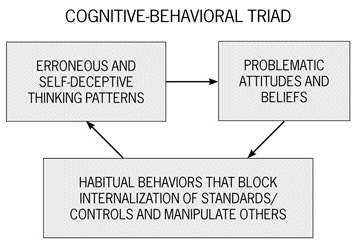
\includegraphics[scale=.4]{Simon_character_5}
\end{figure}

%------------------------------------------------------------------------------%

\subsection{Engaging Effectively \& Intervening Therapeutically with Disturbed Characters}
``As mentioned in an earlier chapter, persons with disturbances \& disorders of character require very different therapeutic interventions than do individuals suffering from varying degrees of neurosis. Neurotics need \textit{insight} into the \textit{unconscious} emotional conflicts that underlie their symptoms. Disordered characters, on the other hand, need \textit{corrective} emotional, cognitive, \& behavioral experience. Their maladaptive behavior patterns, \& the erroneous thinking \& attitudes that help foster them, need to be directly but benignly confronted \& corrected (preferably, at the very moment they occur). They also need to practice or rehearse more adaptive ways of thinking \& behaving. Genuine change always begins in the \textit{here \& now} encounter. This can occur in the context of a therapist's confrontation during a session, or any other encounter with an individual willing to address the necessary issues \& behaviors. Change also has to be reinforced from time to time in many different venues.

There are many principles a therapist needs to employ to effectively promote change in disturbed characters. These same principles must be observed by anyone who wants to deal more effectively with these individuals \& avoid victimization by them. For this reason, I've deliberately attempted to make the principles \& techniques advanced in this chapter fairly simple \& straightforward. In so doing, I hope to help anyone unfortunate enough to know a disturbed character to deal with him or her in a more effective, potentially constructive manner. It should also help you assess whether attempts at promoting change (professional or otherwise) are making any headway.

Many therapists aren't well trained in the art of confronting \& correcting maladaptive interpersonal styles. Some actively resist the notion of confrontation. Many others have experienced frustration \& failure in their work with disturbed characters, especially if they primarily adhere to \& therefore attempted to employ the philosophies \& techniques common to traditional psychotherapeutic approaches. As I say time \& time again in training workshops, \textbf{\textit{trying to treat a disordered character with traditional psychotherapy is like a neurologist trying to perform delicate brain surgery with a dentist's appliances}.} Some tools -- as good as they might be -- simply weren't designed for use in certain circumstances. My years of experience have demonstrated to me that the tools developed to treat neurosis are ineffective at best, \& \textit{potentially harmful} at worst, when the therapist's task is to help ameliorate character disturbance. But because many therapists are still primarily versed in \& adhere to traditional paradigms, they tend to write off disturbed characters as simply nonamenable to treatment. The reality, however, is that character disturbance can be treated, \& often treated fairly effectively, if the right approach is adopted. But when it comes to treating character disturbance -- just as when engaging disturbed characters in everyday encounters -- almost all the ``rules'' are different.'' -- \cite[pp. 188--189]{Simon_character}

\subsubsection{Common Attitudes \& Misconceptions Impairing Therapeutic Understanding \& Intervention}
``Whether you're a therapist attempting formal intervention or a lay person simply trying to understand \& deal with a problem character, some common beliefs \& misconceptions can hinder your efforts. Most of these are in large part the result of the lingering legacy of traditional psychology principles, their subsequent acceptance by the general public, \& their continued dominance among professionals.

The allegiance many still afford to traditional perspectives has always perplexed me. I've heard many claim that they find traditional paradigms infinitely more ``humanistic'' \& benign than behavioral or cognitive-behavioral approaches. But it was the traditional paradigms that advanced such notions as these: ``cold'' detached mothers were responsible for producing autistic children; ``mixed-message''-giving mothers created schizophrenics; \& young girls displaying bizarre behaviors suggestive of incest or other forms of sexual abuse were really children who couldn't come to terms with their own unconscious lust. These days, one would hardly think of such perspectives as humanistic or compassionate. \& most of us regard the postulates mentioned above as ridiculously uninformed. Yet, for some reason, other questionable \& unsupported principles that flow from the very same frameworks that spawned such unfounded beliefs are still accepted by many as valid \& useful metaphors.

Now, I have mentioned before that some principles of traditional paradigms are still potentially very useful when you're dealing with a raving neurotic. But dealing with a disturbed character is much different business. The following are the axioms I've come to believe are the most important to remember:
\begin{itemize}
	\item They \textbf{already ``see,'' they simply ``disagree.''} So many people, including therapists waste considerable time \& energy trying to get disturbed characters to ``see'' the wrongfulness or harmfulness of their ways. They operate under the misguided notion that, despite the fact that the disturbed character has probably heard the same things from a thousand different people a thousand times before, they still simply don't understand the error of their ways \& will finally see the light if the therapist imparts information in a newer, clearer, more cogent way. They fail to realize that most often the disturbed character already understands very well what principles society wants him to accept, but he's simply, for various reasons, still resistant to internalizing those principles. So, successful engagement \& intervention requires primarily that the other party simply set firm behavioral limits \& expectations for any involvement with the disturbed character, \& confront his truth distortions \& responsibility-resistance tactics when he  displays them. Then, when the disturbed character shows even a slight willingness to modify his thinking or behavior, he can be reinforced for so doing.
	\item \textbf{How they feel is not nearly as important as how they think \& act.} Needless attention is often afforded to how disturbed characters must be feeling \& how that might bear upon their actions. When working \& dealing with disturbed characters, it's important to pay far more attention to the kinds of thinking patterns \& attitudes they display, as well as the behaviors they might engage in that block internalizing pro-social values \& standards. Their feelings are not the issue. They may claim so, \& may also use their feelings to justify their actions. But their feelings are not the main problem. How they think \& how they act are what matters most. Once these issues are addressed sufficiently \& successfully, attention can be directed to emotional issues, if necessary.
	\item \textbf{Change occurs in the here-\&-now.} Here's how you know you're making any headway with disturbed characters: If they're willing to make any changes in their thinking patterns or behavior \textit{at the very moment those problematic patterns appear, \& you confront or challenge them about them}. Sometimes, their apparent willingness to modify their behavior is purely superficial \& meant to appease (this is the tactic of ``giving assent''). However, it's a start, \& it can still be reinforced even as you insist on progressively more sincere efforts down the road. When your encounters are still largely dominated by the tactics outlined in the previous chapter, you know the disturbed character remains actively resistant to change. When the tactics become less frequent \& less intense, you might indeed be witnessing some authentic change.
	\item \textbf{Remember: position, position, position.} It's very important to keep in mind that most disturbed characters constantly jockey for a position of advantage in all their encounters, \& that the ``fight'' for maladaptive dominance often begins before they even enter the therapy room or engage with you. So, it's extremely important to set the ``terms of engagement'' very early on (more about this later). It's just as hard for most therapists to adopt an authoritative, confrontational, \& directive stance in therapy as it is for most people to take early charge of their encounters with disturbed characters. But anyone is any kind of relationship with a disturbed character, including a therapist attempting to facilitate change, must be willing to assert expectations, enforce limits \& boundaries, \& employ maximum leverage right from the outset. In traditional therapy, the therapist remains accepting while the client sets the agenda. When dealing with disturbed characters, you must remember that power simply can't be entrusted to those who will almost certainly abuse it. This is a very hard principle for many therapists to accept. They tend to see all efforts to assert authority or control as ``counter-therapeutic.'' But with disordered characters, just the opposite is true. It's imperative that the power rest with the person most inclined to exercise it responsibly. Modeling the responsible, principled use of power is a crucial task for a therapist dealing with a disturbed character.
	\item \textbf{Endorse \& enforce values, principles, \& standards.} The ``old therapy'' was deliberately non-judgmental, positively regarding, \& open. The purpose was to establish an atmosphere in which even the most guarded \& ``hung-up'' individuals could feel safe enough to bare their souls, \& in the process come into conscious contact with the parts of themselves that they had for too long repressed. Disordered characters need to know that \textit{not} anything goes; also they need to understand precisely what values, principles, \& standards you expect them to abide by when interacting with you. Nothing is as potentially corrective or therapeutic as making clear what the values \& principles of responsible behavior are. You must stand up for them firmly, setting \& enforcing appropriate limits \& expectations with regard to behavior.
	\item \textbf{Know, honor \& use the power of confrontation.} Confrontation has taken a ``bad rap'' in recent years. Confrontation doesn't mean hostility or belittlement. Confrontation brings a legitimate issue to the fore \& deals with it. It's pointing directly at the 800-poound gorilla in the room that many so often choose to ignore. I simply can't stress enough why being willing to confront is so important. For years, clinicians wrote off personality \& character disturbances as untreatable. They simply never addressed the core dynamics of a person's dysfunctional style. E.g., they might focus on a person's early childhood trauma, ``anger'' issues, ``fear'' of commitment, or ``insecurity'' without every directly confronting the penchant for habitually seeing himself as superior \& entitled, or for exploiting \& abusing others. Is it any wonder that the core dynamics of his personality remained unchanged? The fact is that the core dynamics defining dysfunctional personality style were rarely ever confronted, which is a significant part of why they went uncorrected.
	
	Confronting in a firm \& unwavering way, even in the face of a barrage of tactics from the disturbed character, is a true art. This is especially because it's so difficult to do in a truly benign \& ultimately loving way. But that's the heart of effective cognitive-behavior therapy with a disturbed character. It's not about the person, his worth, or image. It's about the \textit{behavior}, purely \& simply. That's where the focus needs to be. We must call the disturbed character out on it. Do it dispassionately, but do it nonetheless. Expect him to resist \& to use every tactic in the book to make you think you're unjustified in taking your stance. But do it. It's the only way change has a chance.
	\item \textbf{Don't accept anything at face value.}  Disturbed characters lie, ``con,'' \& manipulate a lot. The most disordered of them do so for no apparent reason. For years, clinicians as well as researchers have not adequately reckoned with this reality. Researchers will blindly incorporate self-report measures into their studies without due skepticism, \& draw conclusions that are unreliable. Clinicians will often accept without question their client's reports, not thinking that they might be feeding into a game of impression management or being misled about the real problems that need to be addressed.
	
	I once consulted to a women's penal institution that, out of necessity, hired a psychiatrist who had never worked with character-disordered individuals before. After he had unadvisedly prescribed a fair number of controlled substances to several of the inmates, I visited with him. I asked what led him to conclude that 1 woman really needed the prescribed popular drug Valium. He recounted his interview with the woman \& the ``depression \& anxiety bordering on desperation'' she reported, as well as the history she gave of being told by many doctors that she ``needed'' the drug. I asked him if, in his own mind, he had ever questioned the veracity of her report. His rely absolutely stunned me. ``Why would she lie?'' he asked. You see, in his fashionable outpatient practice, people usually didn't come banging on his door for help unless they had good reason to do so, \& unless they were in genuine pain. They didn't typically lie to him. He had worked with neurotics for most of his professional life, \& adhered to traditional perspectives. It was beyond his imagination that a person would put on a tearful display '\& exaggerate their symptoms as part of a con game to ``score'' some drugs that would be a real hit with the other inmates, \& could be ``sold'' at a premium price. He couldn't fathom that the pathetic-looking person he had tried to help was later bragging to others about how easily ``duped'' he could be.
	
	When I 1st started working with disturbed characters, I believed not only most of what they told me, but also the traditional psychological explanations for what made them do the things they do. I believed, e.g., that abusers must have been abused themselves; that ``bullies'' were really cowards ``underneath,'' struggling with self-esteem issues; \& that braggarts were really ``compensating'' for feelings of insecurity. What I didn't know is that disturbed characters are keenly aware of how good neurotics like me tend to think. So, they often told me what they thought I wanted to hear. But over time, the more I checked \& cross-checked reliable collateral information about their histories, the less the things they told me made sense. I gradually learned to be more skeptical. Sensing the skepticism, they would often ask what it was I wanted or expected them to say. This was their way of saying that they'd be willing to ``give assent'' to my expectations while still avoiding the simple truth. Only when they knew for certain that I demanded only the truth, the whole truth, \& nothing but the truth did they start to ``come clean'' with me in any significant way.
	\item \textbf{Take charge \& take charge quickly.} Remember, the disturbed character can't be trusted to direct the encounter responsibly, or to wield power or control conscientiously. You must be prepared in advance for your engagements, \& have in mind the rules, expectations, boundaries, \& limits you want observed. You must also be willing to enforce these from the very outset of your encounter. This is especially true when dealing with the aggressive personalities who lack internal brakes \& who go through life like bulls in a china shop. In workshops, I also use the analogy of a locomotive on a mountainside with no brakes. You have to stop such a train when it 1st starts to roll. Because it gathers momentum quickly, if you wait even a little while to act, you're certain to get run over.
	\item \textbf{Frequently Misused Psychology Terms.} Seeing one's way clear to intervene effectively with disordered characters is not only a matter of abandoning ineffective approaches \& adopting a more efficacious paradigm. It's also a matter of correctly labeling \& interpreting events. Unfortunately, many mental health professionals erroneously apply certain terms \& interpretations to the behaviors frequently displayed by disturbed characters. In my workshops, I humorously introduce a ``Top 10 List'' of the most frequently misused terms in mental health (I have actually included an 11th one because of its relevance). The list below should be especially helpful to professionals trying to intervene with disturbed characters. But because these terms have been so widely spread among the general populace, the lay person should find the clarifications below useful as well.
	\begin{enumerate}
		\item \textbf{Denial (vs. lying).} I introduced this topic earlier. A phenomenon traditionally labeled denial is in essence an unconscious ego defense mechanism. It's the psyche's natural way of protecting a person's conscious mind from the experience of unbearable emotional pain. It's a ``this just can't be happening'' kind of reaction to an event or circumstance that occurred too suddenly, with such intensity, or was of such an unusually emotionally painful character that the person simply cannot accept its reality without going to pieces. Generally, denial is a temporary psychological state that breaks down with time \& acceptance. \& true denial can happen w.r.t. a person's behavior pattern, also. This is especially true when the behavior is so unusual or so ``out of character'' that the person simply can't believe he or she did it.
		
		Unfortunately, many times both professionals \& lay persons alike misuse the term denial. I frequently hear people say that someone is ``in denial,'' implying that subject is in some sort of altered psychological state with the conscious mind being unconsciously prevented from seeing the reality of a circumstance. In fact, the person purported in denial is simply lying.
		
		Lying to avoid punishment is not denial. Neither is lying to control the impression another has of you. Lying to oneself is also not the same as denial. Lying is lying. Denial is something else. Sometimes, habitual liars even begin to believe their lies. Still, this is not the same as denial.
		\item \textbf{Acting Out (vs. acting up).} This is arguably the most misused term in mental health. In fact, the definition of this term has been modified in various texts \& professional articles to such a great extent over the years that it bears little resemblance to its original meaning. Technically, the term refers to unconscious inner emotional conflicts expressed through actions as opposed to other types of bizarre symptoms. Here is an archetypal example:
		
		After laboring for several days, \& staying up all night the night before to complete the task, a man puts a business report on his boss's desk. In typical fashion, the ever-demanding boss retorts: ``Well, it's about time. \& it had better be good!'' Upon leaving the boss's office, the man utters under his breath, ``That son-of-a-bitch.'' Then he enters the men's room \& begins washing his hands -- \& washing his hands -- \& washing his hands. He washes until his hands are red, raw \& blistered. He wants to stop but he can't. He has developed a compulsion or ritual. What's worse, he's completely unaware of the connection between his under the breath comment about his boss, the guilt that this evokes, \& the compulsion he feels to make himself ``clean'' again. This is an example of a person acting out the internal war between his \textit{id} that would like to punch his boss's lights out \& his overactive \textit{superego} which demands that he be clean of the stain of such unpardonable urges. So, he washes. His actions are the behavioral manifestation of his inner conflict.
		
		Clinicians \& others often use the term acting out to describe when disordered characters are ``acting up.'' Acting up is not necessarily acting out. Most often, it's simply misbehavior. The term started being misused for 2 reasons: 1st, instances of acting out are not as clear cut as the one outlined above; \& 2nd, for a long time psychodynamic explanations about human behavior were so dominant that almost every behavioral problem was simply assumed to represent the outward manifestation of some inner emotional conflict. There are indeed times when a problematic behavior really represents a form of acting out. E.g., a truly depressed youth might be angry over the breakup of his family but conflicted inwardly about his anger. So he might display his frustration through defiant actions that, in a manner completely unconscious to him, keep him from directing even more anger inward (thus becoming more seriously depressed) or toward family members (thus potentially alienating them). His defiant actions might draw his family's attention to him \& his problems, thus potentially re-uniting his emotionally-separated parents in a cause to save their child. This kind of situation could still be regarded quite appropriately as a case of acting out. But, of late, the term has become over-expanded in meaning to the point of genuine absurdity. Now, almost every instance of misbehavior is referred to as some kind of ``acting out,'' \& the term has found its way into our everyday lexicon. There's even a popular TV commercial for a behavioral therapist's ``proven formula'' for curing your child's ``acting-out'' behavior at school. I cringe every time I hear it. There are many forms besides the one I mentioned earlier that true acting out can take. But, for the most part, acting up (misbehaving) is not acting out.
		\item \textbf{Defensive (vs. aggressive or combative).} Here's 1 of the most frequent comments I hear from partners in abusive relationships who consult me as a therapist: ``Every time I say something to him, he gets so defensive.'' The term ``defensive'' as used in common parlance reflects how traditional notions about the inner workings of the human psyche have been so widely but erroneously accepted by the general public. Most of the time, when my clients talked about the ``defensiveness'' of their partners, they were really describing wanton, intense, \& deliberate \textit{combativeness}. Their partners were behaving in a clearly aggressive manner; but, buying into the traditional notion that no one would engage in such behavior unless feeling in some way under attack, they viewed the behavior as defensive in character.
		
		Here's what generally happens in an abusive relationship (where power is unevenly distributed \& the disordered character has the upper hand): Whenever the abused party tries to assert himself, the disturbed character quickly brings out an arsenal of psychological weapons to browbeat the other party into a position of subordination \& submission. It's combat, pure \& simple. \& it's not combat necessarily rooted in a perception that one is under attack \& has no choice but to defend oneself. One could say that the disturbed character feels his ``position'' threatened \& acts to remove the threat; but once again this stretches a metaphor beyond the range of its usefulness \& accuracy. What's more, buying into this inaccurate perspective only makes the neurotic more likely to feel like the bad guy \& cave in. As soon as the neurotic begins to feel like he's the one responsible for inviting the disordered character to feel bad (i.e., the neurotic begins to feel like he's the aggressor), he's very likely to retreat, \& allow the real aggressor to regain the upper hand. In fact, the neurotic surrenders the potentially level playing field with the aiding \& abetting of traditional psychology.
		\item \textbf{Shame (vs. embarrassment at or distaste for being exposed).} Therapists often assume that a client won't admit a problem because he feels too much shame \& is ``in denial'' as a result. They then seek to guide the client with gentle encouragement \& acceptance  through a lengthy period of overcoming that denial (which may or may not actually occur). But what therapists often fail to consider is this: Not wanting to admit problems, \& not wanting others to know you for the character you truly are, can be rooted in a host of other reasons other than genuine shame.
		
		I was once a guest at another therapist's group therapy for seriously disturbed characters. I sat passively \& listened to group members spew ridiculous excuses for some of the most reprehensible behaviors. After the session, I asked the therapist why some of the lies, obvious errors in thinking, \& various irresponsible behaviors I witnessed weren't immediately challenged. He was a therapist overly immersed in \& aligned with traditional paradigms. He stated that he had to be very careful to pace his confrontations because all of his clients must certainly be dealing with high levels of shame about their behaviors, \& were still very much in various stages of denial as a result.
		
		Let's take a moment \& scrutinize this scenario carefully. We have here a group of disturbed characters, most of whom share similar core beliefs, similar patterns of behavior, \& a similar degree of comfort with those attitudes \& behaviors despite society's disapproval of them. What could possibly be shame-evoking about displaying those attitudes, ways of thinking \& behaviors with a bunch of like-minded individuals? Sometimes, there might actually be someone in the group (especially the therapist) who doesn't share the same beliefs \& attitudes. In that case, you might observe a person being hesitant to self-reveal. But such a hesitance need not necessarily be rooted in genuine shame. A person can be apprehensive about self-revelation for a variety of reasons besides shame, not the least of which is potentially losing the game of impression-management. Shame is a genuine feeling of not liking the person you are. It can actually keep a person from doing things that most would regard as a negative reflection on one's character. \& remember, 1 of the hallmarks of disturbed characters is their pathological lack of shame.
		\item \textbf{Splitting (vs. the tactic of dividing \& conquering).} Therapists tend to misuse the term splitting the most. Splitting is a very rare \& primitive ego defense mechanism: A person unconsciously divides a reality -- far too traumatic to reckon with as a single entity -- into 2 or more separate mental images or constructs. E.g., a child who is severely emotionally abused, but occasionally showed affection by the same parent, may mentally ``split'' that parent into internal images of ``good parent'' \& ``bad parent.'' This permits the child to reconcile conflicted emotions by loving the good parent while hating or fearing the bad parent. Victims of horrendous abuse, who feel such self-loathing that they literally cannot stand themselves, might even split their psyches into several parts. This defense, when carried to an extreme, might even result in forming multiple personalities.
		
		What many therapists erroneously label ``splitting,'' however, is the conscious, deliberate, manipulation tactic of ``dividing \& conquering,'' or creating dissention between others as a way of gaining advantage over them. Children learn this tactic early. If mommy says ``no,'' they go to daddy \& playing the pleading game. Don't even mention that you already asked mommy, \& daddy might give you what you want. If you're in an institutional setting, \& you have problems with authority anyway, try \& divide 1 camp of the staff against another. Professionals often mislabel this behavior ``staff splitting.'' It's a very unfortunate misuse of the term, \& it's not a benign misuse either. An underlying assumption is that the behavior is prompted by the classic \& unconscious ego defense mechanism when, in fact, such ``splitting'' is a conscious \& deliberate offensive power tactic.
		\item \textbf{Passive-aggressive (vs. covert-aggressive).} Passive aggression is another of the most misunderstood \& misused terms in mental health. I addressed this earlier in this book, but it bears repeating. Aggression is the forceful energy we all expend to survive \& prosper. It usually involves attempting to secure a desired goal, to remove obstacles in the way of achieving those goals, or to remove perceived threats to our well-being. Our language reflects our deep-seated awareness of the true nature of aggression. We say things like, ``If you want something, you have to fight for it''; or when we encourage the sick or infirmed to rally their resources \& do battle with their cancers, infections, or other diseases. Humans have always done a lot of fighting. It's a big part of life. When we're not making some kind of love, we're generally waging some kind of war.
		
		How we fight is another matter. It's important to recognize that aggression is not synonymous with violence. Indeed, aggression can be undisciplined \& destructive. Aggression can also be carefully tempered with concern for the impact on others, \& can be potentially quite constructive in the amelioration of human misery. That's what assertive behavior is all about. Aggression can also be purely reactive: an immediate, instinctual response to a genuine threat. But aggression can also be predatory, or, as some researchers prefer, instrumental. Such aggression is neither prompted by fear or anger, \& is not in response to a threat. Rather, it's rooted purely in desire, is strictly ``offensive'' in character, \& the goal is victimization. Aggression can be overt. I.e., it can be out in the open, without pretense, apology, or attempt to conceal. Aggression can also be covert. I.e., it can be carefully cloaked so that aggressive intent is concealed from open observation. Covert aggression is at the heart of much interpersonal manipulation \& emotional abuse. People often get conned \& abused by others because they fail to spot their aggressive intentions \& behaviors until after they've already been victimized.
		
		1 relatively benign form of covert aggression is passive aggression. Passive aggression is, as its name suggests, aggression through passivity. It's not answering your mate when you're mad at him. It's not returning a phone call when you don't really want to connect with the other person. It's ``forgetting'' once again to pick up the dry cleaning the partner you're mad at asked you to pick up. It can be a fairly powerful \& frustrating strategy when carried to extremes. When Gandhi's followers simply stood fast \& would not move out of the army's line of fire, although many perished, their ``passive resistance'' eventually brought an occupying empire to its knees. Most of the time, however, passive aggression is a relatively self-defeating strategy, especially when it comes to getting what you need in a relationship.
		
		Most of the time, when I hear people use the terms ``passive-aggressive'' or ``passive aggression'' what they really means is ``covert aggression.'' The term ``passive-aggressive'' is used incorrectly to describe the subtle, hard to detect, but yet deliberate, calculating \& underhanded tactics that manipulators \& other disturbed characters use to intimidate, control, deceive, \& abuse others. That's what covert aggression is all about. Although this kind of aggression is often subtle or concealed, there's absolutely nothing ``passive'' about it. It's very active, albeit veiled aggression.
		\item \textbf{Passivity (vs. uncooperativeness).} Sometimes, disturbed characters who are deliberately, but not openly, resistant to cooperation are viewed as ``passive'' \& unassertive. Deliberate uncooperativeness needs to be labeled for the combative stance that it is. Resistance-prone characters don't need to be taught assertive skills as much as they need to be confronted about their maladaptive penchant for fighting.
		\item \textbf{Co-dependence (vs. dependence or abuse).} Perhaps no term is as overused \& misused as this term. The term was originally intended to describe the phenomenon by which members of an addict's family of can end up having their lives just as much controlled by the addict's substance of choice as the addict himself. So, whereas the addict becomes substance-dependent, the family members often become co-dependent with the addict on the substance of choice. The lives of co-dependent individuals become so governed by the addict's addiction that they inadvertently give up control of their own lives in service to the addict, thus unintentionally ``enabling'' the addict's dysfunctional behavior.
		
		It would take another entire book to address the strengths \& weaknesses of the co-dependency metaphor. Suffice it to say that the phenomenon the term was meant to describe does in fact exist. However, the term is often misapplied to behaviors \& situations it was never initially meant to define. Most especially, the term is erroneously used to describe ``dependency,'' mutual dependency, or even ``abuse.'' When disordered characters enter into relationship, abusive \& exploitative behaviors inevitably follow. When a therapist ``frames'' a disordered character's refusal to accept financial responsibility, deliberate disinterest \& neglect of family needs, \& excessive burdening of his partner as a case of ``dependence'' upon that partner, the entire nature of the relationship becomes distorted. When both the abuser \& the victim are seen as ``co-dependent' instead of the abusive party being correctly identified as such, \& the dependency of the unassertive party (who would likely have set \& enforced limits or even left the relationship long ago if it weren't for their excessive emotional dependency) goes unnoticed, the therapist is likely to promote a substantial amount of ``enabling'' of the abusive situation.
		\item \textbf{Help (vs. chasing \& enabling).} Long ago, 1 of my colleagues, who just happens to be a clinical social worker, told me a joke that pokes some fun at 1 of the stereotypes sometimes ascribed to persons who enter the helping professions. It seems there were 2 social workers walking down a big city street when a mugger on a bicycle rode by \& snatched their purses. The social workers took off running in a fruitless attempt to catch up with the robber, all the while shouting to passers-by: ``Stop that Man! $\ldots$ Stop Him!! $\ldots$ He's obviously in serious need of our help.''
		
		Help is the offer of assistance we extend to those who truly need it \& ask for it. Help is not chasing after someone to give them something we think is of value even when they haven't asked for it \& show no appreciation for it. Help is not visiting the same issues with someone over \& over again when they've already heard the same thing a million times \& haven't displayed any motivation to change. Whenever we chase after people to give them something we value but which they disdain, we only reveal our own psychological pathology. \& whenever we repeatedly put ourselves in a position to be ignored, exploited, or abused, we only ``enable'' \& encourage disturbed characters to continue their dysfunctional ways.
		
		I know far too many therapists who sell themselves \& their potential tools of empowerment far too cheaply. You have to remember, the disturbed character always wants something for nothing. That's part of what's at the heart of his character defect. Whenever a therapist (or a person with whom he is in a relationship) tries too hard (under the guise of ``help''), he enables the disturbed character to continue not working on the necessary tasks of change. In the process, he loses any hope of being afforded any respect. In 1 of the vignettes presented later in this chapter, you'll get an idea of what rightfully constitutes the ``help'' people need in their relationships with disordered characters.
		\item \textbf{Needs (vs. wants).} There are some things that every living creature needs to survive \& prosper. Humans have evolved to the point, \& learned enough over the centuries, that with only a modicum of mutual cooperation, most human needs can be met with relative ease. In fact, we've reached the point in many advanced societies where we take our basic necessities for granted. Some of us, however, are never satisfied. We want, want, \& want still more. Sometimes the things we want are the very last things we truly need (e.g., 1 more piece of pie, 1 more relationship on the side, 1 more luxury condo). Neurotics are notorious for being too apprehensive about getting their basic needs met, \& the therapist's job is often to help them assert themselves \& learn how to secure their legitimate needs. But when therapists try to help disordered characters find less disruptive ways to get the things they want but don't need, \& don't challenge their greediness directly, disaster almost inevitably follows.
		
		Disturbed characters are more than happy to plead their case \& solicit your understanding. They almost always want an ``ear'' \& to have their point validated. They don't want to have their attitudes, beliefs, \& ways of doing things challenged. They certainly don't want guidance, direction, \& correction. But those things are exactly what they need the most.
		\item \textbf{Symptoms (vs. signs).} When a person reports his subjective experience of distress to a professional (e.g., ``I feel achy all over''), it's called a symptom. When a person displays a physical abnormality, a particular behavior or pattern of behavior, or any observable \& objective manifestation of a reality, it's called a sign. The fact that the terms are often misused by professionals is problematic enough. But the problem is exacerbated by the fact that character-disordered individual most often give distorted \& sometimes deliberately dishonest reports about their experiences \& circumstances. So, the symptoms they report cannot be trusted. Instead, the clinician often needs to take what clients say with a grain of salt. The therapist must be extra mindful of the \textit{signs} they display, especially the cardinal or most essential signs (e.g., distorted thinking patterns, responsibility-avoidance \& manipulation tactics) that signal the presence of character disturbance \& other pathologies.'' -- \cite[pp. 189--206]{Simon_character}
	\end{enumerate}
\end{itemize}

\subsubsection{Empowered Engagement with Disturbed Characters}
``In my 1st book, \textit{In Sheep's Clothing}, I outlined some of the general rules anyone (layperson or therapist) must observe to empower themselves in relations with disturbed characters, especially manipulators. Those general guidelines include:
\begin{itemize}
	\item Letting Go of Harmful Misconceptions -- especially this tenet of traditional psychology: that everyone is essentially the same \& struggling with fears \& insecurities.
	\item Becoming a Better Judge of Character -- not necessarily by doing a thorough professional character analysis, but at least by knowing the basic personality features of the persons you're dealing with. Also, decide where they likely lie on the neurotic-character disordered continuum.
	\item Knowing Yourself -- well enough to understand the needs, insecurities, \& belief systems that might put you at risk for being taken in by an unscrupulous character.
	\item Knowing the Twisted Thinking Patterns \& Tactics -- some people use to avoid responsibility \& manipulate others. It's important to know them well, to recognize them the moment they're employed, \& to respond to them appropriately.
	\item Investing Energy Only Where You Have Power -- by choosing battles carefully, avoiding losing battles, \& never succumbing to the temptation to take on the burden belonging to someone else. Take charge of your own behavior. Set your own limits \& expectations. Leave the burden for change where it belongs -- on the person with the behavior problem.
\end{itemize}
In addition, I outlined some specific rules to observe to remain maximally empowered in any encounter. These rules include:
\begin{itemize}
	\item Never accept an excuse. If a behavior is wrong, the reasons for it are irrelevant.
	\item Judge actions, not intentions. Never second-guess a motive or accept a promise on the surface. Actions speak much louder than words.
	\item Set limits \& expectations, \& do so very early on in any encounter.
	\item Make requests that are clear, simple, \& direct.
	\item Accept only clear, simple, \& direct responses.
	\item Stay focused on the here \& now.'' -- \cite[pp. 206--207]{Simon_character}
\end{itemize}

\subsubsection{The Paradigm Necessary for Change}
``For years an ongoing debate has occurred abut whether therapy even works, or if it does work, what makes it work. The question becomes even more salient when we're talking about therapy for disturbed characters -- arguably, the most difficult individuals to treat.

In my work over the years, I have found that the art of therapeutic intervention with disturbed characters goes far beyond merely adopting a cognitive-behavioral approach (as opposed to traditional psychotherapeutic approaches). Some of the most important principles are outlined below:

As mentioned earlier, the cardinal principle of intervention with disturbed characters is that \textit{change occurs in the here-\&-now}. I.e., every single encounter with a disturbed character not only reflects their interpersonal dysfunction's nature but also presents an opportunity for corrective emotional \& behavioral experience. Every interaction, therefore, is an opportunity for change, learning, \& growth. If you're ever going to facilitate change, you must literally seize the moment, \& refuse to let it go until something different takes place.

My experience includes consulting with therapists of many different training backgrounds, as well as giving numerous workshops \& seminars. This has made me aware of how rarely the basic tenets of cognitive-behavioral therapy (CBT) are actually employed, despite the facts that there is fairly widespread knowledge about the paradigm \& so many purport to adhere to it. Most clinicians know that CBT is the right answer when you ask them what approach is superior in dealing with character disturbance. Most will even say they employ it. But often, when I scrutinize this claim, I learn that \textit{cognitive} strategies are indeed employed (albeit only at times), whereas behavior modification techniques are usually not employed at all.

Almost every therapist I know has at least a mild aversion to behavior therapy. Most seem to regard it as ``cold'' \& mechanical, \& ultimately ineffective because it does not focus on the ``whole'' person. Some ardently believe it does not attend to the ``underlying dynamics'' traditional approaches assumed to motivate behavior. Even the common terms associated with behavior therapy, such as generalization, reinforcement schedules, cue saliency,  response conditioning, send shivers up the spine of most therapists I know. But behavior therapy has demonstrated its effectiveness \& even superiority fairly convincingly, \& adding the cognitive component to the paradigm only enhances its effectiveness further. Unfortunately, however, although many therapists will say they do CBT, what they really do is often a mixture of CT (Cognitive Therapy) \& traditional PT (psychotherapy). Is it any wonder why many end up pulling their hair out when trying to make headway with a disturbed or disordered character?

Many of the techniques employed in the here-\&-now process of emotional, cognitive, \& behavioral counter-conditioning are potentially just as useful to the layperson as they are to a therapist. So it might be helpful to see these principles at work in some typical therapeutic encounters. The following altered vignettes are based upon actual case, each of which exemplifies many of the principles we've covered. The commentaries provided after each vignette are meant to elaborate on the principles employed.

These vignettes depict sessions typically conducted in an outpatient setting. The principles used in these mostly 1-on-1 encounters can also be applied to group-based interventions \& treatments. Sometimes it's even easier to call attention to erroneous thinking patterns, \& to confront responsibility-resistance behaviors, when there are others in a group familiar with these things.

The 1st vignette depicts a real diagnostic interview with an adolescent male \& his mother. The young man had been having behavior problems at home \& at school. Despite his young age, he was already showing signs of significant character dysfunction. As is generally the case, his mother insisted he come to see a professional. As I typically do, I met initially with both together. The vignette is useful for illustrating the principles outlined earlier in this book, showing how to gain leverage with \& deal effectively with character disturbed individuals. As with all of the vignettes in this book, some of the material \& identifying information is altered so as to ensure complete anonymity. However, all of the essential psychological dynamics have been painstakingly preserved. I should mention that, although I mean to illustrate methods \& principles, I do not mean to suggest that my interventions were perfect. I always see things I would do differently when I review case vignettes. So, this vignette not only illustrates what general principles should be observed, but also what things should be avoided to deal effectively with the disturbed character. After presenting the vignette, I'll discuss some of the general principles \& issues that beg further exploration.'' -- \cite[pp. 207--210]{Simon_character}

\paragraph{Vignette \#1: A behaviorally disturbed adolescent brought in by his mother}
\begin{itemize}
	\item Therapist (addressing adolescent 1st): What brings you here today?
	\item Adolescent: I have no idea.
	\item Therapist: Are you trying to tell me that you're the kind of person who will go places or do things without knowing why?
	\item Adolescent: I don't know what you want from me anyway. If you wanna know anything, ask her (looks glaringly at his mother)!
	\item Therapist: I haven't decided just yet whether to consider your input on things, or simply talk to your mother \& base my opinions \& suggestions solely on what she tells me. But I thought I'd ask you about things 1st.
	\item Adolescent: She thinks I have an attitude problem.
	\item Therapist: I'm not sure what you mean by ``attitude problem.''
	\item Adolescent: ``She's always doin' stuff $\ldots$ makes me mad all the time. Sometimes, she makes me real angry.
	\item Therapist: Of course, she has no power to \textit{make} you mad. \& anger is a normal, healthy human emotion. It's rarely a problem in itself. So, I'm still wondering what the problem really is.
	\item Adolescent: I told you. She knows just what to do to piss me off. \& she does it all the time.
	\item Therapist: I accept that you need to say that. Maybe you even believe it, I don't know. Maybe you just want me to believe that you believe it. But you should know that I never accept notions like anyone can \textit{make} you feel or do anything. Your feelings belong to you. I also won't accept that anger in itself can be a problem. Maybe you can tell me what you typically \textit{do} when you get angry with your mother.
	\item Mother: He curses. He says all kinds of hateful things.
	\item Therapist: I think I might understand why you might be willing to speak for your son. But for now, I want to speak to him directly \& have him speak directly to me, okay?
	\item Mother: I'm so sorry. I didn't mean to $\ldots$ (looks ashamed \& hangs head down)
	\item Therapist: What do you \textit{do} when you get angry with your mom?
	\item Adolescent: You heard her.
	\item Therapist: It's not my intention to fight with you.
	\item Adolescent: I'm not fighting.
	\item Therapist: Of course you are, \& have been since you got here, perhaps even before that. \& I know that you know that. It's quite apparent that you're here against your will. Still, I don't want to fight with you. I will be open, honest, \& direct. I will not be disrespectful. There are obviously some problems here, \& I'd like to learn more about them. I'm willing to deal with only your mom about them if I have to, but I'd like to get your input.
	\item Adolescent (huffing heavily): This whole thing is because I shoved her once -- okay? \& it was all because she got right in my face. I've told her a million times not to do that.
	\item Therapist: So, you are saying that you have been physically aggressive with your mom.
	\item Adolescent: I just touched her. She wouldn't leave me alone. She knows that sets me off.
	\item Therapist: Do you often rationalize -- i.e., make excuses for -- being aggressive?
	\item Adolescent: I'm not making excuses.
	\item Therapist: Of course you know what an excuse is \& when you're making one, so we certainly won't fight about that. My question is only whether you tend to make these kinds of excuses for your aggressive behavior \textit{often}.
	\item Adolescent: Only when I have good reason.
	\item Therapist: I should tell you that unless it's to defend your life against a real attack, I will never accept any excuse for aggressive behavior.
	\item Adolescent: Does that go for everybody?
	\item Therapist: For everybody. Has your mother eve aggressed against you?
	\item Adolescent: Well $\ldots$ no.
	\item Therapist: So, you are not really the victim here. Your mom says or does things you don't like, \& you tell yourself you have the right to aggress against her.
	\item Adolescent: But she knows what she does \& how it makes me mad.
	\item Therapist: You seem determined to make yourself out to be the victim \& cast blame on your mom. When you aggress against your mom, she's the victim, not you.
	\item Adolescent (more forcefully): She never has anything nice to say. She's constantly on my back. It's always this \& always that.
	\item Mother: Maybe he has a point. It could be partly my fault.
	\item Therapist: What do you think is your fault?
	\item Adolescent: I don't know. Maybe because I just don't know what to do anymore. I've tried taking away privileges, talking to him calmly. He just seems to get so mad. It's hard to talk to him. Maybe I end up saying too many negative things.
	\item Therapist: The issue I want to focus on right now is the aggression. How often has he been aggressive with you?
	\item Mother: Not that often.
	\item Therapist: How often would that be?
	\item Mother: 4 or 5 times, I think. But nothing as bad as the other night. That's why I called you. I was really afraid he might hurt me that time.
	\item Therapist: What do you do when he aggresses?
	\item Mother: Try to calm him down. Try to talk to him. Try to understand what's making him act that way.
	\item Therapist: You don't have the power to calm him down. What do you do to protect yourself?
	\item Mother: Do you think I need to?
	\item Therapist: If you don't do what you have power to do, \& keep trying to change things you can't control, you'll get angry, frustrated, \& depressed. Then, you won't think straight or have the energy to handle the situation properly. You have power over your behavior. That's why I asked you what you do when he aggresses.
	\item Mother: What can I do?
	\item Therapist: Have you considered calling the police?
	\item Adolescent (bursting out \& glaring at mother): That's it! Now, I suppose you'll go hollering to the cops \& get me in trouble with the law any time I say a cross word!
	\item Mother: Don't you think that would be a little much. A little cruel?
	\item Therapist: I think what your son just did is cruel. \& covertly aggressive (manipulative). He's casting himself as the injured party while at the same time trying to beat you up with guilt \& shame -- insinuating that you're the kind of person who will over-react \& get him into unwarranted trouble over a trivial matter. What do you usually do when he tries to intimidate you like this?
	\item Mother: (starts to cry, says nothings)
	\item Adolescent: That's what she does.
	\item Therapist (to adolescent): Do you ever let yourself think of just how wrong \& harmful it is for you to fight like you have in here today. Rationalizing behavior you know is wrong, but making excuses for it anyway; minimizing the seriousness of some of your actions; using tactics such as making yourself out a victim; intimidating your mother; spending all that energy to have the upper hand \& not doing 1 minute's work to learn how to control yourself. Do you ever think about how wrong all of that behavior is?
	\item Adolescent: (gets a bit somber, remains mute)
	\item Therapist: I'm going to give you my opinions now about what I see as problems; what I think each of you needs to do about 
	it; \& what I'll be willing to do to help.
	\item Mother: Okay.
	\item Adolescent: (looks up \& sit attentively)
	\item Therapist: I think things are upside-down in this family. This young man acts like the boss \& sometimes bullies, (addressing mother) \& you don't know what to do to gain the upper hand. Have you ever been in a situation like this before?
	\item Mother: (with head down low \& in a soft voice): Uh $\ldots$ my 1st husband.
	\item Therapist: So, you need to get much better at recognizing \& dealing with aggressive behavior. This young man will naturally fight for the things he wants \& test all the limits. He doesn't know yet how to handle power, \& you haven't learned yet how to effectively wield it.
	\item Mother: I don't want to make him hate me.
	\item Therapist: You don't have the power to make him hate you.
	\item Mother: Maybe he will anyway.
	\item Therapist: Are you saying if you stop tolerating abuse, set limits, \& provide direction, you're worried your son will hate you for it?
	\item Mother: Maybe.
	\item Therapist: \& you might tolerate abuse just to avoid feeling hated?
	\item Mother: I just want him to know I love him \& to appreciate me.
	\item Therapist: You don't have power over his attitudes or feelings.
	\item Mother (tearfully): What if he just leaves?
	\item Therapist: You don't have power over what he does, just how \textit{you} respond to it. You have the power \& responsibility to get a good example, to set limits, expectations \& consequences, beyond that you have no power. But the power you do have is significant.
	\item Mother: What should I do? 
	\item Therapist: I'm willing to provide you supportive counseling, \& help you learn better ways to empower yourself \& to be better able to handle yourself in the difficult job of parenting this young man.
	\item Adolescent: You mean I don't have to come (looks glad at this point)?
	\item Therapist: I mean, at this time, I'm choosing not to work with you.
	\item Adolescent: What if I want to come anyway?
	\item Therapist: Should the time come when I think it could possibly be of benefit, I might agree to see you.
	\item Mother: So, should I come next time?
	\item Therapist: Yes. I'll give you some things to look over that can serve as a springboard for the work we will be doing.
	\item Adolescent: I think I'll come next time, too.
	\item Therapist: You may come, of course, but I will not see you. You can sit in the waiting room \& read a magazine.
	\item Adolescent: All you'll do is talk about me \& say things behind my back that aren't true, \& I won't be here to defend myself.
	\item Therapist (turned toward mother but speaking loud enough for son to hear): We will focus only on the issues I spoke about earlier. We will leave him out of it.
	
	(Turned toward son): I think it would be nice for us to visit under the right circumstances. I have a lot of things you may find useful in making important changes in your life.
	\item Adolescent: I know what you're trying to do. You're trying to get me to change by making me feel bad. Well, it won't work!
	\item Therapist: I don't have the power to change you. I only have the power to assist people who want to change. As I see it, there are things both of you need to change. \& I respect that you don't see the need for doing things differently just now. So, for the time being, your mom \& I will work on the things she wants to change.
	\item Adolescent: I still may want to come sometime.
	\item Therapist: I think that would be really nice under the right circumstances. When I think the time is right, \& if I'm convinced it could be of benefit, I'll be glad to give it a shot.
\end{itemize}
Let's take a step-by-step look at the interpersonal processes going on in this vignette. Both of the individuals in my office that session had their own reasons for being there. I almost always ask individuals making an appointment to see me what their purpose is in seeking me out. The adolescent's response to my opening question is telltale. His brief response is packed with tactical maneuvers \& reveals much about his as yet unspoken agendas. He responds by saying he has ``no idea'' why he's there. Keep in mind, I rarely listen that closely \textbf{\textit{to}} what a person says. I usually listen \textbf{\textit{for}} the kinds of things he or she might say (i.e., the tactics of manipulation \& impression management they might employ), \& what the underlying agendas most probably are. Now, it's remotely possible that the exact purpose of this specific visit wasn't spelled out by his mother, but I feel it quite safe to assume that this young man has a pretty good idea why he's in a counselor's office. So, I make the following suppositions, merely on the basis of his opening remark:
\begin{enumerate}
	\item He's using the tactic of feigning ignorance (i.e., ``playing dumb'').
	\item His use of the tactic means he's fighting. He doesn't really want to be there, \& he certainly doesn't want to submit himself to my authoritative counsel (i.e., he's already fighting with me \& wants to control the encounter).
	\item He's of insufficient character to be entrusted with the leadership role in his interactions with me. I need to set all the terms of engagement, \& assume an authoritative stance quickly.
\end{enumerate}
Now, my response to this young man's opening remark is not typical of how I operate these days. The question I asked had a more provocative tone than I usually find necessary. Sometimes provocative questions are necessary \& helpful, but I don't use them as often anymore. By implying that he is trying to cast himself as someone who simply goes where he's told to go \& does what he's told to do without any awareness of the purpose, I'm casting him as a passive or deferential type of person, when in fact I suspect quite the contrary. This provocative technique can be used with individuals who are, in fact, quite aggressive in interpersonal style; but they attempt to cast themselves as passive, \& to cast those who are suffering in relationships with them as villains. By using this technique, I'm signaling to this youngster that I believe him to be actively engaged in impression management \& manipulation, as opposed to being willing to engage in discourse. By stymieing that effort, I increase the chances he'll take a different course.

Next, this young man attempts to direct attention to his mother, \& to take more solid control of the interview process. He also puts her on notice with a glaring glance (i.e., uses the tactic of covert intimidation). My response is to assert who will control the interview process, \& what kind of behaviors I will or won't tolerate. Such things always need to be done firmly but matter-of-factly, with no displays of hostility or malice. Asserting control over the process must also be done without hesitation. I also use the ``leverage'' technique of suggesting 2 possible outcomes, one clearly less desirable than the other, \& present the youngster with a choice. By insinuating that he might not be given a voice in matters that concern him, he is prodded to make a better choice. I don't engage in this level of leverage anymore because it is too akin to manipulation, i.e., making a covert or veiled threat. So, although I move quickly to establish that I make the decisions about the process, I don't red-flag outcomes as leverage. I merely assert that I'll be making a decision regarding with whom I will work.

In the case at hand, the young man takes the bait, \& for the 1st time offers up some information. The way he frames it, however, is to insinuate that his mother harbors an erroneous belief that he has a problem with his ``attitude'' (engaging in covert belittling). His tactics are to again divert attention to his mother, to cast her as a villain, \& to cast himself as an innocent victim.

I take the opportunity to invite the young man to elaborate on just what the ``attitude'' issues are, but he quickly blames his mother for ``doing stuff'' \& ``saying things'' that upset him. He uses the tactic of overgeneralization to exaggerate any legitimate issues (i.e., ``she is \textit{always} doing stuff''), \& tries to put the blame for \textit{his} responses squarely on her. I then firmly take a stand behind this principle: No one bears responsibility for behavior other than the person engaging in the behavior. I also take a stand on the principle that human emotions, including anger, are not the cause of human suffering. I put the focus squarely on thinking patterns \& most especially behavior, not emotions.

As I increasingly pin the youngster down on the relevant issues, \& have nearly successfully zeroed in on the specific problem things he does, look who comes to the rescue! Good ol' mom speaks up \& says what he easily could have admitted himself some time ago. I begin to learn a lot about her \& her penchant for rescuing. When I benignly confront her about that, her behavior of wanting to crawl into a hole \& hide tells me almost everything else I need to know about her \& her own character.

I then get back to the matter of confronting the problem behavior for which the mom dragged this young man into my office in the 1st place. Along the way, I confront the resistance of this young man directly. I indicate that I have no intention of becoming ensnarled in a fruitless power struggle. He eventually acknowledges that the proverbial straw that broke the camel's back, prompting the visit to my office, is that he has become physically aggressive with his mother. He then launches a literal barrage of responsibility-avoidance \& manipulation tactics: He trivializes (i.e., uses the tactic of minimization by saying ``only once'' \& ``not hard'') the importance of his physical misconduct, \& attempts to re-assign blame to his mother (.e.g, ``only because she was in my face''); he casts himself as a victim, \& rationalizes (makes excuses). Disturbed characters use these tactics because they're generally quite effective (exemplified by some of the mother's later statements). I can't count the number of times workshop attendees have told me that they might strive to find out if, in fact, the mother ever really did get in this lad's face. But that successfully leads them off the topic at hand; it shapes their impressions of the situation in the manner the young man is seeking to shape impressions. I make it clear, however, that I never entertain an excuse for physical assault. It's wrong, period. I make it crystal clear the principle I stand on, \& that I'll accept no excuse for violating the principle.

An important thing to note: When I next confront the young man's excuse-making, I don't accept his ``denial'' (i.e., lying) about the fact that he's been physically aggressive. I don't buy into the potentially fatal notion that he's most likely ashamed of himself \& can't believe he's really done such a thing; or that his conscious state is so altered that he truly thinks he hasn't done it. Rather, I assume he knows full well not only what he's done, but that society generally frowns on such actions, \& would negatively appraise his character. So, I don't assume his ``denial'' is motivated by the pain of guilt or shame. I instead assume that he's actively engaged in defiance of a principle, resisting submission to the notion that such behavior is simply not okay. He's simultaneously attempting to manipulate me into a more favorable assessment of his character, not wanting me to think of him as the type of person who's comfortable aggressing against people simply because they called attention to his character flaws.

I then witness what happens when the young man more intensely takes aim at his mom, using a barrage of tactics \& casting her as the villain. Eventually, she caves. She accepts not only the notion that she's at fault, but that she's at least partly responsible for his aggressive conduct. She's willing to take on too much responsibility; he's taking none -- an archetypal dysfunctional relationship \& a perfect example of what happens when the overly conscientious neurotic is in a relationship with a person of deficient character.

Eventually I decide that the person to work with 1st is mom. I do so for 3 main reasons:
\begin{itemize}
	\item[a.] She's in more immediate pain \& discomfort \& will be motivated to seek relief;
	\item[b.] She's fairly neurotic (she has character issues, but on balance her over-conscientiousness exceeds the level of her character deficiency) so she's more amenable to traditional counseling;
	\item[(c)] The balance of power in the family is pathologically skewed \& needs re-alignment. Mom is not supposed to be perfect, just the authority figure. Instead, she's in the 1-down position. I don't want to ``enable'' the balance to remain unhealthily skewed. \& I'd like to facilitate the process of mom gaining mental \& emotional strength for both her own benefit \& that of her son. Despite the fact that he's nearing adulthood, he desperately still needs authoritative guidance.
\end{itemize}
In fashioning the initial plan of treatment, I also had to take into serious consideration the mom's unhealthy emotional dependency, \& how she might tend to overly rely on my support as opposed to doing what's necessary to empower herself.

Traditionally-oriented therapists might easily be uncomfortable with the fact I did not initially conduct therapy sessions with the ``identified'' client (i.e., the adolescent brought in by his mother). The traditional approach would be this: Set an atmosphere of positive regard \& willingness to ``help''; then the young man would eventually ``overcome his resistance'' \& forge a therapeutic alliance with me. However, I might offer some fairly provocative points of explanation: (1) It was particularly respectful of me to accept this young man at exactly the place that he was w.r.t. receptivity to change. (2) His mother bears primary responsibility for guiding his character formation \textit{\&} she really needs help right now. (3) Denying a visit to the adolescent, setting strict terms of engagement, standing up for principle, making clear that my support was freely available under the right terms -- all this was, in fact, 1 of the most \textit{corrective} \&, therefore, \textit{therapeutic} things I could have done. (4) My commitment to principle, willingness to call both parties out on their various pathologies, \& work over a several-month period with the mother demonstrated my professional credibility as well as my trustworthiness. This greatly enhanced the likelihood that the young man would seek me out when the time came to want help for himself, if necessary.

Now, I did eventually see this young man professionally. In fact, I saw him several times. The 1st time was when he begged for a session, primarily because he'd lost a lot of leverage with his mother, \& was seeking to re-tilt the balance of power. I saw him once but refused him regular counseling at that time. The 2nd time, he was having some problems at college \& was in danger of being tossed out. I agreed to see him, but again I limited contact to the initial visit. Why? His motivation was primarily to alleviate his immediate distress. He had insufficient desire to work on the character traits that created the problem in the 1st place, \& he was well aware that I don't engage in ``crisis management,'' but rather ``character development.'' He was aware, however, that my door was always open to him for the right kind of work.

He came to see me when his 1st marriage was on the rocks, making some degree of investment in therapy; but when he came to grips with how much work (i.e., changing) he had to do, he departed prematurely. After the breakup of his 2nd marriage, a bitter divorce, self-sabotage in his 1st career, \& a few other major failures, he came back again, this time to really work. \& work he did. I should say that, in addition to his brief earlier visits with me, he had made the rounds of counselors, including psychiatrists, \& was offered all kinds of opinions about the nature of his problems \& how to overcome them. He was given just about every kind of diagnosis along the way, from adult ADD to Bipolar Disorder, \& was prescribed various medications. His relationship difficulties were framed as anything from ``fear of intimacy'' to ``low self-esteem.'' But he himself had the answer when he brandished the worksheets I had long ago given his mother on thinking errors \& responsibility-avoidance tactics. Waving them in front of me, he stated empathically, ``This is me. These sheets say it all. These are the kinds of things I've always done. I've always had this kind of thinking \& I've always used these kinds of tactics to kid myself \& manipulate others. My whole life has been a train wreck just waiting to happen, \& I always knew it but wasn't ready to give in (note how he frames the issue as a matter of capitulation -- NOT insight). I just want to make my life different now. I hope it's not too late.''

So, he knew in his heart what the problem was all along. \textit{Awareness} was \textit{never} the issue. \textit{Acceptance} or the lack thereof was the major obstacle, finally overcome. \&, as has been proven to me countless times, I believe this is why he came back to me instead of to someone at the other places he'd been: He knew he could trust me to confront the key issues directly, without undue whitewashing or politically-correct mis-framing. He knew where I stood \& what my principles were. I'd confronted him on what I believed to be his most important issues before, \& he knew early on whether or not my assessment was on the mark. This meant he had good reason to trust me, \& there's no possibility of a truly therapeutic relationship without trust. If I'd tried to candy-coat his behavior by attributing it to low self-esteem, depression, a chemical imbalance, or past trauma, I would have had absolutely no credibility. In all of his encounters with me, I must have sounded like a broken record, always espousing the same principles \& never succumbing to his vigorous attempts at impression management. When the time was right, he knew he could count on me for the honest confrontation \& authoritative guidance he needed. I gladly obliged him. Because his motivation was internal, the effort on my part from that day forward was minimal.

If this were only 1 shining example of success in a sea of treatment failures, it would certainly not serve as a support for the philosophy I advocate. But I've been around long enough now to see scenarios similar to this one repeated many times.

The following is another vignette that illustrates well the thinking patterns \& attitudes common to the disturbed character. It also shows the tactics they habitually \& automatically use to resist accepting responsibility, \& to manipulate \& manage others' impressions. It is a sort of ``complete'' vignette containing a few snippets from several different, but very similar, interviews woven into the principal character's dialogue.

The vignette is of an interview between a prison social worker \& an inmate. The inmate is a female who has been in trouble with the law on numerous occasions, but has come to prison for the 1st time. The prison social worker is attempting to learn something about the woman's background to assist placing her in programs that will help her earn the earliest possible parole.'' -- \cite[pp. 210--222]{Simon_character}

\paragraph{Vignette \#2: A newly incarcerated female with a history of antisocial conduct \& drug abuse}
\begin{itemize}
	\item Interviewer: Tell me how you happened to come to prison.
	\item Inmate: To tell you the truth, I think my probation officer had it in for me. She just doesn't like me.
	\item Interviewer: How is that?
	\item Inmate: Well, I was keeping my appointments \& doing everything I was supposed to do; but then I caught a silly drug charge, \& she revoked me \& sent me here.
	\item Interviewer: A drug charge?
	\item Inmate: Yeah. I got pulled over \& the cop found a little weed in my car. They didn't even ask me whose it was or how it got there.
	\item Interviewer: So you were charged with possession?
	\item Inmate: Actually, they got me for distribution.
	\item Interviewer: Why distribution?
	\item Inmate: Well, because some of the weed was in little bags.
	\item Interviewer: Why in little bags?
	\item Inmate: (Shrugs her shoulders)
	\item Interviewer: How many bags?
	\item Inmate: About 50.
	\item Interviewer: 50 is quite a few bags. Would you say that you were probably going to distribute those bags?
	\item Inmate: Not that day.
\end{itemize}
Let's take a good look at this very illuminating scenario. Here we have a social worker trying to do something potentially quite helpful for this woman. In order to get her into the right program in a timely manner, the social worker needs to know what this woman is all about. She needs to know her criminal history, the kinds of problems \& issues to address, \& how serious the problems are. Gaining access to the right programs \& completing them with a favorable rating can result in considerably less time of incarceration for the inmate. So, the social worker is trying to ``help.'' Meanwhile, from the very outset this inmate is engaged in a game of impression management, manipulation, \& responsibility-avoidance. It's exemplified by the thinking patterns she displays \& the tactics she uses.

When the social worker asks why the woman has come to prison, the 1st thing the inmate does is blame her probation officer. (Actually, the very 1st thing she says is ``to tell you the truth,'' which in the case of a disturbed or disordered character, represents your 1st clue that a lie is about to follow.) She paints a picture of herself as a compliant, dutiful probationer who had the ``bad luck'' to be assigned a probation officer who didn't like her, \& so recommended revoking her probation for no good reason. She then casts herself as the victim of even worse luck by being stopped by a police officer (she skirts the issue about why she was stopped) who stumbled upon ``a little weed'' in her car. She also implies (misleads through insinuation) that, had the officer asked about how it might have gotten there, she might have been able to offer an exculpating explanation. So right off the bat, she externalizes the blame, minimizes the nature of her wrongdoing, \& casts herself as a person of generally good character who has been treated unfairly by the system.

Now, you should know that the social worker has this woman's complete criminal record \& history in a fairly thick informational ``jacket,'' \& has been perusing through it while asking the woman questions. Also, upon minimal further probing, more of the truth comes out (although there is still a substantial amount of lying by omission \& distortion going on). Given these facts, it would have been much easier, simpler, \& less time consuming for the inmate to have simply acknowledged to the social worker that she has a habit of drug trafficking, \& got ``busted'' once again -- \& that's why she's in prison. All this will be learned in short order anyway, so one has to wonder why this woman simply doesn't fess up.

Therapists aligned with traditional psychology models would automatically assume that this woman feels too guilty \& ashamed ``underneath it all'' to simply self-reveal so bluntly, \& is probably still ``in denial'' to some degree about the nature of her life \& circumstances. But what the woman has to say later in the interview challenges those kinds of assumptions:
\begin{itemize}
	\item Interviewer: So I'll bet you're going to think twice about having anything to do with drugs again when you get out, huh? I'm going to recommend that you get into the substance-abuse treatment program. That'll look good on your record, too.
	\item Inmate: I don't need any treatment. I ain't got no real problem. I'm not an addict or nothin'. Look, everybody does a little weed sometimes, \& there's nothing wrong with that. Everybody I know does weed. \& I ain't no big time dealer, either. I know lots of people who sell all kinds of heavy stuff for lots of money, \& they didn't catch the charges I got or get the time I got. The cops take bribes from the real pushers \& leave them alone. Anyway, I didn't catch a lot of time, so I'll be out soon enough. I'd rather do my time \& get out than have to be in 1 of those [more colorful language deleted here] programs where they make you talk about God \& higher powers \& [stuff] like that, \& make you say you're an addict \& you don't know how to run your own life anymore.''
\end{itemize}
Diehard traditionally-minded therapists would still insist that this woman's apparent ``denial'' of the extent of her ``problems'' is proof of her underlying emotional pain. But the reality is more likely this:
\begin{enumerate}
	\item This woman does not feel badly about her behavior. She only regrets that her life has now been interrupted.
	\item She has no genuine remorse, not only w.r.t. the wrongfulness of her behavior, but also for the potential negative impact it had on others \& society at large. The social worker asked her about who was caring for her 2 young children. Her response was that it was no big deal because her  mother had always pretty much cared for them. That fact reflects on her lack of concern for the impact of her conduct. Again, traditionally-minded therapists might frame the fact that her mother has to care for the kids as an instance of ``dependency.'' But ``using'' others as vehicles to enable your irresponsible lifestyle is not the same as true dependency.
	\item She's going to do what she has always done when she gets out, because she hasn't submitted herself to the principle that her behavior is wrong or harmful. She's still at war with principles she knows society wants her to accept.
	\item She attributes the causes of her misfortune to external sources, not to her wrongful thinking \& behavior.
	\item She detests the notion of subordinating her will to any kind of ``higher power'' whether within some kind of program or not.
	\item She's nowhere near uncomfortable or troubled enough emotionally or mentally to be motivated to change her modus operandi.
	\item This woman has been around. She's familiar with drug treatment programs \& the tenets of several of them. She also understands that other people take issue with her attitudes \& beliefs toward drug use. There's nothing at this point that anyone can say that she hasn't heard a thousand times before, \& that might make her ``see'' what she's doing \& its consequences. She already \textit{sees}, but she still disagrees with some fundamental principles about how to function in a civilized world.
\end{enumerate}
A major question in most people's minds might be this: Why doesn't this woman just say from the beginning what she obviously knows, \& then more clearly admits toward the end of the interview? Of course, the traditional assumption is that she's ``in denial'' which blocks her insight. But it should be evident, when taking a careful look at the whole of this encounter, that she's simply accustomed to using certain tactics to justify her behavior, to resist change, \& to manipulate the impressions of others about her character. In fact, such tactics often work, at least in the short-run. So, she uses the tactics to keep doing as she damned well pleases, without concern for the impact of her behavior on others. It should be noted that this woman is 1 of many inmates who, when given a choice between submitting to some kind of correctional program to gain earlier release, will forego that opportunity. When they are released, they don't want anyone looking over their shoulder (i.e., a parole officer) to whom they'll have to answer. Remember what I said about aggressive personalities: They find it anathema to be in a situation in which they have to recognize or submit to a higher authority.'' -- \cite[pp. 222--226]{Simon_character}

\paragraph{Vignette \#3: An adult male referred for evaluation by another therapist}

\begin{itemize}
	\item ``Client: Hey, how's it goin' George? Well, today's the day, huh? The big shrink's gonna tell me what he thinks (smirks).
	\item Therapist: As I promised you last time, I am going to share with you my opinion about what I see as a problem. \& I'll give you some suggestions about what you would need to work on in therapy. Then, I will give your therapist a copy of my report.
	\item Client: Well, what's the verdict, doc? You're a doctor of what $\ldots$ philosophy $\ldots$ psychology? Is that like a real doctor, or what?
	\item Therapist: As we talked about the 1st time, I'm a psychologist. I'm not a medical doctor. All of my training is in psychology. My area of specialty is personality \& character. As we have discussed this at length before, perhaps we'd better get on with my assessment.
	\item Client: Go ahead. Shoot.
	\item Therapist: I think that, for you to have fewer of the kinds of problems you've been having, \& in order to be a better person in general, you need to make some changes in the kind of person you are -- some basic changes in your personality. At your age, that won't be easy, but I think that's what you'll need to do.
	\item Client: What about my personality?
	\item Therapist: Mostly, you lack good ``brakes.'' Also, you tend to think too much of yourself, \& you tend to pay too little heed to others in your life \& their needs.
	\item Client: I'm not sure what you mean, bad brakes.
	\item Therapist: I think you understand that when you want something, or want to do something, you don't hesitate or stop \& think about it 1st. In fact, you don't stop at all. You don't back-up, back-off, or give-in when you should. You're in full-throttle mode in the very times you really need to be thinking about applying the brakes.
	\item Client: \& you can tell all this after just a couple of visits?
	\item Therapist: As we discussed earlier, I consider much more than just our visits, which is why I've consulted with your therapists, interviewed some of your family, looked at your history, \& given you some tests. I've also made some important observations about the kinds of attitudes you display \& behaviors you exhibit. I consider my opinion accurate.
	\item Client: Even if no one else has ever told me that before? Dr. Brady thinks I probably have depression. But you think I'm just a bad person. So, he's wrong \& you're right, huh?
	\item Therapist: I can't speak for anyone else. I'm giving you my opinion. \&, of course, you didn't hear me say you were a bad person. I said you're a person with poor brakes. I mean exactly what I said.
	\item Client: Dr. Brady says my anger is a symptom of depression. Maybe that's what it is. Maybe all I need is a pill.
	\item Therapist: Anger can indeed be a sign of depression, especially when it is out of character for the person. But I've carefully reviewed your history. There were many times when you were on a mission of sorts -- taking no prisoners -- fighting hard to get what you wanted -- \& you weren't angry at all. Many times, when you showed anger, it seemed more to intimidate those who opposed you -- a tactic as opposed to a genuine feeling. You seemed to do whatever you had to do to get what you wanted without care for whom you hurt, \& you ended up losing in some way. If you had put on the brakes, you might have really won. Then you got upset because you'd made a mess of things. How long have you had a problem putting on the brakes?
	\item Client: I just don't see how you could be so sure after just meeting me. You don't really know anything about me. I mean, you're saying some pretty heavy things here. Besides, I like me. Lots of people like me. They love me at work, \& I do great at my job. Make good money. But you tell me I'm all messed up.
	\item Therapist: You ask how I can be so sure. I think you would know better than anyone else whether any of what I have said to you makes sense. \&, of course, you know that I'm not suggesting you need to change \textit{everything} about yourself. What I am saying is that, as an aggressive personality, you have to learn when \& when not to pull out the stops, \& when \& when not to put on the brakes. You also need to get a more balanced sense of self-worth. It seems to have really riled you that anyone might have accurately assessed your character. You actually helped confirm most of my hunches when you started out this session using the tactic of leveling; i.e., trying to intimidate me by subtly denigrating my credentials, trying to throw me on the defensive. I think you need to stop all the very destructive behavior that I outlined for you on the worksheets I gave you, \& which I'm sending to your therapist as well. If you don't work on correcting those things, you'll keep hurting people \& making a mess of your relationships. It won't be easy, but you can do it. \& you can start by doing some things differently right here \& right now.
	
	Now, my question to you, if you remember, is how long you've had this problem $\ldots$ I mean, with your brakes.
	\item Client: My whole life.
\end{itemize}
The scenario depicted above illustrates several of the points I've already made about the nature of encounters with disturbed characters, especially the egotistic \& aggressive personalities.

1st, posturing \& jockeying for position was evident from the very beginning of the encounter. As I've mentioned before, in the client's mind, the ``fight'' had already started, even before the formal encounter began.

2nd, you can expect folks who like who they are, \& who are relatively entrenched in their way of doing things, to resist the notion that they need to change. They're very happy to frame whatever is going wrong in their lives as almost anything else (e.g., a depression) than to face the daunting task of real change. Unfortunately, sometimes professionals can enable that resistance.

3rd, at some level, the disturbed character really knows what the real issues are. He will eventually demonstrate respect \& some degree of amenability if the person confronting him stands on principle \& holds ground. Just because clients resist, saying all kinds of things \& using all kinds of tactics, doesn't mean they don't deep down know the truth. If you don't nail them on the truth, they have absolutely no reason to respect or trust you.

4th, basic personality tendencies can change if you'll actually give them some attention. \& change ways occurs in the here \& now. When the client in the vignette above finally capitulates (it might have been an instance of ``assent'' only), he is in fact doing something different from what he usually does. This small step is actually a big deal, which needs to be recognized \& reinforced. That would send a message to him that the world will not come to an end if he considers modifying his \textit{style} of relating. The more the dysfunctional aspects of his style are confronted \& corrected, \& the more reinforcement he gets for modifying his usual modus operandi, the more he will grow \& change. If a lot of time were wasted in therapy talking about the things that depress him, as well as his fears or insecurities, not much about his personality would change.

This case underscores a couple of very important points made earlier about some disturbed characters, especially the egotistic \& aggressive personalities. Remember, it's always about 3 things: position, position, \& position. Right from the outset, this individual tries to put me in a place he wants to prescribe for me. He doesn't want to see me as an authority. He especially doesn't like the notion that I might have some advantage over him by ``having his number.'' He uses the tactic of ``leveling'' not only to even the field of contest between us, but also to put us on an equal level of stature (e.g., he calls me by 1st name \& engages in subtle mockery of my professional status). He also can hardly allow himself to believe that someone else could have the upper hand in an encounter with him \& could be so astute as to see through his game of impression management, \& get to th core of his character issues. But in the end, it is the truth \& the willingness to stand up for it that saves us both from further, destructive combat.'' -- \cite[pp. 226--230]{Simon_character}

\paragraph{Vignette \#4: A mother seeking a 2nd opinion about how to help her daughter}
``This very brief vignette helps illustrate how some of the principles of traditional psychology have not only gone too long unquestioned by professionals, but also have been generally accepted by laypersons, much to their detriment in trying to understand \& deal effectively with disturbed characters.
\begin{itemize}
	\item Client: She must have really low self-esteem. She'll tell me I think she's stupid whenever I try to offer constructive criticism. She says her teacher has it in for her, too. She says the teacher's a jerk \& lets the other kids pick on her, \& she's the one who gets in trouble when she defends herself. She can't possibly feel good about herself. She gets so defensive whenever I try to correct her.
	\item Therapist: What do you mean ``defensive?''
	\item Client: If I say the slightest thing about her behavior, she flies off the handle. She'll say I hate her, or that I never have anything good to say about her. She'll kick \& scream. Sometimes she'll hit me. I don't want her to feel so badly that she has a meltdown. So, I keep my distance. But I know she needs help. The other therapist says it all stems from her low self-esteem. But I don't know what to do.
	
	Like many, this mother (as well as her child's therapist) believes that no one would react so intensely to criticism unless ``underneath it all'' they didn't have a poor opinion of themselves. Also, she appears to believe that the child perceives the efforts others have made to help her as an ``attack'' on her worth, meriting a ``defensive'' (albeit spirited) response. But in my work with this family, it became quite clear that this child was anything but self-unsure in character or ``defensive'' in posture. She was the consummate fighter, \& had reason to be confident that she could take on the best of opponents. To be sure, she lacked the wisdom of life experience necessary to see the ultimate shortcoming of her ways. But for now, she perceives herself as winning, \& she feels pretty good about it. So good, in fact, that she's outpaced her mother in strength, power, \& influence. That's a recipe for disaster in any family. Kids can't forge a decent character on their own. They don't have the moral maturity or the wisdom to do it. They need authoritative guidance. With this child, mom ends up backing off, because she knows neither how to interpret nor deal with her daughter's tactics. So, she ends up facilitating the creation of a monster.'' -- \cite[pp. 231--232]{Simon_character}
\end{itemize}

\paragraph{Vignette \#5: A long-term client actively working on his character development}

\begin{itemize}
	\item ``Client: I'm not sure what I need to work on today. It's been a crazy week. \& I'm sure you can tell I'm just a bit hyper today. So, if I start rambling, you'll just have to stop me. No $\ldots$ I already know what you're going to say, I need to stop myself. Okay. I'll try.
	\item Therapist: That's great.
	\item Client: I didn't go to my computer class today because the professor is such a jerk \& has given us a bunch of busy work, \& we've not been learning the really important stuff, anyway.
	\item Therapist: (Gives only a familiar glance)
	\item Client: Okay. I know. I'm rationalizing.
	\item Therapist: So why didn't you go to class today?
	\item Client: I wanted to spend some time with Marcie. She's a lot more interesting! I probably shouldn't have trashed Prof. Bartlett like that, just to make an excuse for choosing time with Marcie over computer class. He's actually an okay guy. \& besides, I probably need to be better about my attendance anyway because I need the grade. I'm actually doing okay, just not as good as I could be.
	\item Therapist: I like how you took ownership of your decisions, both good \& bad. What do you think you'll do to keep yourself on track better?
	\item Client: Well, Marcie's schedule is different from mine. There's a lot of time when she doesn't have class when I do. So, I'm probably going to get tempted to skip again. When that issue comes up \& I make the right choice, I'll treat me \& her to a beer at Charlie's (a popular hangout). When I don't, I'll make myself put in an extra hour of study.
	\item Therapist: That sounds good.
	\item Client: You don't seem all that impressed.
	\item Therapist: You know why I resist being too demonstrative in my support for you.
	\item Client: Yeah. You want me to recognize myself \& not have to depend so much on others to encourage me.
	\item Therapist: Right.
	\item Client: But you can't blame me for wanting you to be impressed.
	\item Therapist: Blame you, no.
	\item Client: But you still want me to recognize myself.
	\item Therapist: Right. This is all about you \& how you value your own efforts to be a better person.
\end{itemize}
Now, this is a young man with whom I had worked for many years since his early childhood. During that time (as is typical for any child going through the process of character development) he developed a fair degree of dependency upon the support, guidance, \& direction he was afforded. There was times that I confronted him directly \& frequently about his various behaviors, tactics, \& thinking patterns interfering with his efforts to build character. But in the end, the material I gave him on his worksheets became his to learn \& internalize. It also became incumbent upon him to be more self-observant, \& to catch \& correct maladaptive patterns as they emerged. Sometimes, when he'd forget to ``catch'' himself exhibiting a maladaptive behavior, a glance from me would be all it took to remind him. My job then turned primarily to reinforcing him for his efforts (like I did with the brief verbal praise in my 1st 2 responses). Eventually, however, even the task of reinforcement had to become his. He is a living example of how the behavioral principles of covert self-monitoring \& self-reinforcement for correcting behavior can be powerful instruments of change.'' -- \cite[pp. 232--233]{Simon_character}

\paragraph{Vignette \#6: A snapshot of a husband \& wife in a joint counseling session}

\begin{itemize}
	\item ``Wife: I want you to do better about not calling me names, cursing, \& belittling me when we have things to discuss.
	\item Husband: \& I suppose you're going to tell me you've never cussed before or anything. There's no winning with you. I can't do anything right. I always end up looking like the bad guy.
	\item Wife: I'm sticking to my issue here. I'm not accepting that this is about me, or which 1 of us is the better person, or that you're a victim in any way. Despite the fact that you've improved on the name-calling, I want you to do better. I just want you to work harder at not calling me names or belittling me when we have a discussion.
	\item Husband: Okay, okay, \textit{okay}!
	\item Wife: \& I don't just want you agreeing to get me off your back [using the tactic of ``assent']. I'm going to be watching for this to get a lot better over time \& to last.
\end{itemize}
The woman in the scenario above ``gets it.'' She anticipates tactics \& is not swayed by them. She has a legitimate concern \& makes a legitimate request. \& she takes ownership of setting her own reasonable expectations \& limits. She has no need for hostility or for defensiveness. She knows what to expect \& what to do. As she mentioned to me many times, life has completely changed for her.'' -- \cite[pp. 233--234]{Simon_character}

%------------------------------------------------------------------------------%

\subsection{Epilogue: Neurosis \& Character Disturbance}

\subsubsection{The Most Pressing Issue of our Time}
``There is an old saying that ``all roads lead to Rome.'' I.e., many issues can be traced to a single source. When you seriously examine our most pressing social problems, whether political, interpersonal, occupational, or even economic, the problems can eventually be traced to impaired individual responsibility. Like it or not, character matters. It affects everything we do, \& character-deficiency lies at the root of many woes we face. Even the biggest financial crisis since the Great Depression was mostly caused by the greed, dishonesty, \& irresponsibility of a handful of character-deficient bankers \& executives.'' -- \cite[p. 235]{Simon_character}

\subsubsection{Where Is the Outrage?}
``For months, the public was subjected to endless warnings about the dangers of a possible swine flu epidemic. Industries \& public agencies rallied. But the problems posed by this virus pale in comparison to the pain, misery, \& social costs incurred every day by the character crisis facing the industrialized world. Yet, we have no public outcry. In fact, we've become all too accepting of the fact that the responsible among us are dwindling in number. We seem to regard it as an inevitable feature of the human condition. We might get outraged when a horrendous character like Bernie Madoff rips off millions of hard-working Americans, but we don't seem too interested in how such a person becomes a problem character in the 1st place. It's important to realize that character disturbance is not only a very serious issue, but also a phenomenon we can actually do something about. But 1st, we must become oriented toward addressing the issue.'' -- \cite[p. 235]{Simon_character}

\subsubsection{The Wrong Way to Attack the Problem}
``For quite some time, western societies have sought legislation solutions to the character-disturbance problem, almost always with unintended, \& sometimes disastrous results. We have more rules on the books than a reasonable person could possibly count, \& we attempt to enforce new rules every day. We behave as if the solution to our ills is more \& tougher rules. But the fact is this: The irresponsible people among us don't pay attention to the rules, nor are they particularly influenced by the potential consequences of breaking them. Those of us who live in a righteous spirit do not act responsibly because of the rules or for fear of breaking them. To make matters worse, however, we are overly \& unfairly burdened by the rules we devise in our fruitless effort to control the irresponsible among us.

To prove the point that trying to ``legislate'' morality almost always has unintended \& sometimes disastrous consequences, I offer the following example: A 7-year-old boy was observed giving a girl at school a kiss on the cheek. This violated the school's ``no-tolerance'' guidelines on ``sexual harassment is an insidious behavior that needs to be dealt with firmly. But the way the rule was crafted defies common logic. \& remember what I said about all roads $\ldots$ Well, here's the reason we can't leave it to principals, superintendents, or school boards, to exercise discretion: We don't trust that people put in those positions will always have the integrity of character, the soundness of judgment, \& the appreciation of shared principles necessary to exercise good discretion. So, we make blanket rules that affect everyone ``equally,'' with ``no-tolerance,'' \& set up firm, inflexible guidelines that all authority figures must follow. (Most states even mandate that judges sentence criminals within certain guidelines.) In the end, we erroneously place our trust in ``the rules'' instead of people -- competent adults we would like to fairly interpret, administer, \& enforce the principles the rules were meant to advance.

Our misplaced trust in rules impairs us from exercising necessary discretion. Also, since we cannot specifically target every possible act of social irresponsibility, many people escape so-called justice because no specific statute covers their alleged act of wrongdoing. So, even though almost anyone with a brain knows that it's wrong to steal, ``con,'' or cheat, irresponsible people spend their time finding ways to do all such things that are not covered by a specific statute. An example of this is the near-collapse of the American capitalization system \& the economic recession (nearly depression) it spawned. There were rules in place to keep ``regular'' banks from engaging in risky behavior with other people's money, but those rules didn't cover financial institutions who largely act like banks but aren't technically banks. Unscrupulous money managers stayed within the law but engaged in horribly reckless behavior for personal profit. Their behavior might not have been illegal but it was reprehensible. All roads lead to $\ldots$

The incessant overburdening of the responsible folks among us will eventually prompt a more wholesale abandonment of responsibility, i.e., leadership burnout. Those who have always taken their social responsibilities seriously are becoming sick \& tired of carrying the burden for everyone else. They'd like a break every now \& then. Some seem to be so endowed with intellectual capacity, endurance, \& the penchant for multi-tasking, they can handle the increasing burden without succumbing to depression \& defeat. But many are not fairing very well under the ever increasing weight placed upon them. They labor with a large sense of unfairness \& resentment about those they carry on their backs. Nature has a way of intervening to stop imbalance. This trend will have to end. \& when circumstances finally force the issue, it will not be pretty.'' -- \cite[pp. 235--237]{Simon_character}

\subsubsection{What's Happened to Punishment?}
``There is a popular perception that punishing people for wrongdoing is simply ineffective. There is a grain of truth to that notion. Punishment is by no means the ideal way of shaping human behavior or building character. Reinforcement is a more powerful behavior modifier. \& nourishing empathy \& teaching mutual regard are better shapers of character. But punishment's recent ``bad rap'' has much more to do with how western societies typically penalize than with the nature \& potential value of punishment itself.

Even when punishment is administrated effectively, it appears to only deter, suppress, or inhibit behavior. It doesn't have the power to eliminate it or curb it indefinitely. So, I'm not advocating punishment as the ideal behavior shaping tool. But the fact that punishment can indeed help humans \textit{inhibit} their behavior (especially by strengthening inhibitory neural networks during the formative years) is of significant value. For punishment to be effective, however, (whether it involves introducing an aversive consequence or removing a positive one), it must meet some specific requirements. It needs to be \textit{immediate} (the optimal interval between an act or impulse \& an aversive consequence is actually somewhat less than 1 second), \textit{certain} (i.e., occurring across a wide variety of situations \& circumstances any time the misbehavior is exhibited), \& of \textit{sufficiently aversive} quality to deter the person from exhibiting the behavior again.

In my quarter century of working with clients ranging from parents \& children to prison inmates, I've seen that punishment is almost never immediate. The neurotics among us have seen to it that the wheels of justice turn exceeding slowly. \& for a variety of reasons we have come to particularly disdain corporal punishment, even though when it's appropriately done during the most appropriate developmental years, it can at least provide an immediate consequence to a child's wrongful actions. Someone who commits a crime will wait months or even years (depending on their resources for appeal) to face the consequence of their conviction. \&, as every criminal knows, getting caught \& actually having to face deserved consequences is anything but certain. The ``system'' is overloaded, jails \& prisons are overfilled, \& all kinds of deals are cut to get out of the rightful consequences of misbehavior. Children learn early how unreliable it is these days that parents, teachers, \& other authority figures will agree, not only on whether a behavior merits sanction, but what that sanction should be. Long gone are the days when children were told that persons in authority were always ``right'' as far as they were concerned; \& that any trouble a child got in with another parent, guardian, teacher, or coach would only be met with stiffer consequences from his or her own parent. Lastly, some of the ways we ``punish'' are so devoid of aversive quality that it's laughable. Despite the salacious \& distorted reports of what life is like in prison, with a few notable exceptions, many inmates enjoy a life behind bars (with free health \& dental care, better \& more reliable housing, clothing, \& nutrition) than they were ever used to in the ``free world.'' So, many criminals not only don't mind coming back to prison, but some even deliberately sabotage their paroles \& probation to regain entry. \& we call this punishment?'' -- \cite[pp. 237--239]{Simon_character}

\subsubsection{The Disappearance of Basic Rules of Human Decency}
``Gone are the days that some very basic rules for decent conduct were known \& respected by a majority. In former days, a child could expect most parents to respond in a similar way to concerns about their behavior. \& they could also expect their parents to back up the observations or the discipline of other authority figures such as aunts, uncles, neighboring parents, or teachers. Beginning with the rebellious `60s, all the rules became much less clear. Now, authority figures in children's lives undermine each other with regularity.'' -- \cite[p. 239]{Simon_character}

\subsubsection{The Right Way to Address the Problem}
``It all starts with individual responsibility. The only time-tested effective training grounds for that is a stable, intact home. Children can only learn to be responsible when they ``bond'' emotionally to caretakers that model for them firm commitment, adherence to principle, \& the willingness to accept obligation freely \& with love \& joy. In their early years, children are very dependent upon their caretakers. This dependency must eventually be overcome, but it also serves a vital purpose early on. A child who depends upon external support will experience unsettlement, anxiety, \& distress when that support is withdrawn. Looking at years of research about the most important factors necessary for kids to emerge as responsible adults, one could rightfully conclude that 2 factors appear of the greatest importance: (1) the children were afforded love \& affection \textit{liberally} \& \textit{unconditionally}, \& (2) support \& approval for their behavior was very \textit{conditional}.

A child who knows in his soul that he is truly loved will not only bond emotionally, but also will become unnerved when sensing parents' disapproval. This is the greatest shaper of character known to exist. A properly bonded child might kick \& scream during various phases of the socialization process; but she will eventually ``cave-in'' to the demands when seeing that the caretaker's discipline is rooted in loving concern. Even those who ``rebel'' as adolescents will eventually come back to the principles they were taught as younger children, especially once they begin learning that their parents weren't as stupid as they once thought.

We don't need more rules, more institutions, more programs, or more psychological experts paid to try \& repair (\& inadvertently ``enable'') the damage done by character dysfunction. Rather, we need to pay attention to our children, \& what really helps their character develop in the 1st place. We must stop divorcing each other so frivolously, take our parental responsibilities much more seriously, agree with \& support one another on the most basic principles of civil behavior, \& instill an appreciation for those principles in our children early on. We must bring back a sense of right \& wrong, as well as a sense of shame. \& when some person, company, or entity engages in behavior that promotes or ``enables'' the erosion of these principles, we should call them out \& let out outrage be known. We should also support all those making genuine efforts to do the responsible thing, backing them not only verbally, but also emotionally \& even financially.'' -- \cite[pp. 239--241]{Simon_character}

\subsubsection{The Need for an Honest Discourse}
``Humankind has always faced challenges to its survival \& prosperity, but today's challenges are particularly daunting. If we're to have a prayer of truly recognizing \& overcoming our difficulties, we simply must do 2 things: People of integrity \& character must come together, \& they must engage in an \textit{honest} discussion of the issues. These 2 requirements are inextricably interdependent. There has to be sufficient integrity of character among those talking (i.e., the participants must necessarily have faced \& overcome their fears, biases, insecurities, \& misperceptions) for the truth of important matters to emerge, \& to be appropriately accepted \& reversed when it does.

All too often these days, concern over political correctness (i.e., how socially ``enlightened'' or acceptable we think others might regard the position we take) \& the tendency to put personal beliefs \& interests ahead of the general welfare impair our ability to conduct an honest discourse \& debate. It's natural for people to strive to advance their causes. But when they distort important aspects of a situation in order to ``frame'' the debate in a manner that gives them an edge, everyone loses. Too often, people let their biases, underlying motivations, \& unholy determination put a self-serving ``spin'' on the issues they seek to confront or address. \& although politicians have raised this tendency to an art form, they're not the only ones too cowardly \& self-serving to acknowledge, speak, \& respect the simple truth.

As individuals, we must become more aware \& honest about the fears, biases, \& distortions that we let close our minds \& impair our judgment. Getting honest with ourselves about who we really are: This is essential for psychological health \& personal growth. \& becoming much more honest with one another about our mutual problems \& concerns is essential to avoiding further social fragmentation \& polarization. Confronting issues \& one another in a frank yet benign way has never been easy. But the bottom line is this: If we don't get honest \textit{with ourselves about ourselves} \& \textit{with one another about one another} \& soon, we're pretty much done.'' -- \cite[pp. 241--242]{Simon_character}

\subsubsection{The Road to Riches}
``There are some things in life whose value is almost impossible to measure. In my life, I've been in many places psychologically, spiritually, \& financially. My present-day life is abundantly rich in many dimensions. But there were times when this was not the case. Looking back on those times, it's sobering to realize how pivotal a role my character defects played in creating \& maintaining the difficulties in my life. I am by no means a person of enviable virtue. I have plenty of shortcomings \& vices. But I owe everything of value I have in my life to reckoning with my most serious character defects, \& making sincere efforts to change. I also owe a supreme debt to those who labored on my behalf to instill any sense of character in me. Some people express gratitude by saying: ``I don't know where I'd be'' without the love \& support of their family, friends, \& other supporters. But I know exactly where I'd be if I hadn't come to appreciate the character-shaping lessons I've been given. I've been in the abyss before. It wasn't pretty. \& I don't want to go back. I know I still have a long way to go. I am still a very flawed creature. But I am determined to continually do better, \& most especially, to \textit{be} better. I'm determined because I know in the deepest recesses of my soul how much character matters. \& I hope that, in some small yet significant way, this book has helped impress the importance of character upon you as well.'' -- \cite[p. 242-]{Simon_character}

%------------------------------------------------------------------------------%

\section{{\sc Shannon Thomas, LCSW}. Healing from Hidden Abuse: A Journey Through the Stages of Recovery from Psychological Abuse}

\begin{enumerate}
	\item \cite{Thomas_psychological_manipulation}. {\sc Shannon Thomas, LCSW}. {\it Healing from Hidden Abuse: A Journey Through the Stages of Recovery from Psychological Abuse}. {\sf[3461 Amazon ratings][2519 Goodreads ratings]}
	
	{\sf Amazon review.} Within every community, toxic people can be found hiding in families, couples, companies, \& places of worship. The cryptic nature of psychological abuse involves repetitious mind games played by 1 individual or a group of people. Psychological abuse leaves no bruises. There are no broken bones. There are no holes in the walls. The bruises, brokeness, \& holes are held tightly within the target of the abuse. {\it Healing from Hidden Abuse} walks the reader through each of the 6 recovery stages researched \& developed by the author. The stages are Despair, Education, Awakening, Boundaries, Restoration, \& Maintenance. A guided Personal Reflections journal is included in the back of the book to help the reader go deeper in their application of the 6 stages of recovery. The journal can be used individually or in a small group setting.
	
	-- Trong mọi cộng đồng, những người độc hại có thể ẩn náu trong gia đình, cặp vợ chồng, công ty, nơi thờ cúng. Bản chất khó hiểu của lạm dụng tâm lý bao gồm các trò chơi trí óc lặp đi lặp lại do một cá nhân hoặc một nhóm người chơi. Bạo hành tinh thần không để lại vết bầm tím. Không có xương gãy. Không có lỗ trên tường. Những vết bầm tím, gãy xương, lỗ thủng được giữ chặt trong mục tiêu bị lạm dụng. {\it Healing from Hidden Abuse} hướng dẫn người đọc qua từng giai đoạn trong số 6 giai đoạn phục hồi do tác giả nghiên cứu \& phát triển. Các giai đoạn là Tuyệt vọng, Giáo dục, Thức tỉnh, Ranh giới, Phục hồi, \& Bảo trì. Một nhật ký Suy ngẫm Cá nhân có hướng dẫn được đính kèm ở cuối cuốn sách để giúp người đọc tìm hiểu sâu hơn trong việc áp dụng 6 giai đoạn phục hồi. Nhật ký có thể được sử dụng riêng lẻ hoặc trong một nhóm nhỏ.
	\begin{itemize}
		\item {\it``Psychological abusers do not take responsibility for their actions, so that must be flung onto someone else.''}
		
		-- Những kẻ bạo hành tâm lý không chịu trách nhiệm về hành động của mình nên việc đó phải đổ lên người khác.
		
		\item {\it``The core inherent faulty thinking of abusers is that everything revolves around them.''}		
		
		-- Suy nghĩ sai lầm cố hữu cốt lõi của những kẻ bạo hành là mọi thứ đều xoay quanh họ.
		
		\item {\it``Abusers like to target people who have something they do not or cannot possess themselves.''}
		
		-- Những kẻ bạo hành thích nhắm vào những người có thứ gì đó mà bản thân họ không có hoặc không thể sở hữu.
	\end{itemize}
	{\sf Editorial reviews.}
	\begin{itemize}
		\item ``Compassionate \& well-researched, a must read for anyone healing from psychological abuse. The warm, conversational writing style \& {\sc Shannon Thomas} professional experience combine to make the perfect recovery resource.'' -- {\sc Jackson MacKenzie}, author of {\it Psychopath Free} \& cofounder of \url{PsychopathFree.com}, an online support community that reaches millions of abuse survivors each month.
		
		-- Từ bi{\tt/}động lòng trắc ẩn \& được nghiên cứu kỹ lưỡng, một cuốn sách phải đọc cho bất kỳ ai đang chữa lành khỏi sự lạm dụng tâm lý. Phong cách viết mang tính trò chuyện, ấm áp của \& {\sc Shannon Thomas} trải nghiệm chuyên môn kết hợp với nhau để tạo nên nguồn tài nguyên phục hồi hoàn hảo.
		
		\item ``{\sc Shannon Thomas} has written an important book about something ugly, hidden, \& difficult to describe. Psychological abuse. How is it possible that 1 person can gain so much power to destroy another person's sense of worth, safety, \& sanity? {\sc Shannon} tells you how, but more importantly, she gives you a roadmap that helps you wake up, break free, heal, \& rebuild your shattered life.'' -- {\sc Leslie Vernick LCSW}, counselor, coach, speaker, \& author of {\it The Emotionally Destructive Marriage} \& {\it The Emotionally Destructive Relationship}.
		
		-- {\sc Shannon Thomas} đã viết một cuốn sách quan trọng về một điều gì đó xấu xí, ẩn giấu, \& khó diễn tả. Lạm dụng tâm lý. Làm sao mà một người có thể có được nhiều quyền lực đến vậy để phá hủy cảm giác về giá trị, sự an toàn và sự tỉnh táo của người khác? {\sc Shannon} cho bạn biết cách thực hiện, nhưng quan trọng hơn, cô ấy đưa ra lộ trình giúp bạn thức dậy, thoát ra, chữa lành, \& xây dựng lại cuộc đời tan vỡ của mình.
		
		\item ``Few writers are able to connect research, experience, \& intuitive understanding as {\sc Shannon Thomas} does in her groundbreaking new book for survivors of emotional \& psychological trauma. In {\it Healing from Hidden Abuse}, you will find not only evidence of {\sc Shannon}'s expertise as a therapist who has worked with clients suffering from the trauma of covert psychological abuse, but also her powerful mastery of the crucial questions that are needed in order to work through the trauma \& heal.'' -- {\sc Shahida Arabi}, author of {\it Becoming the Narcissist s Nightmare: How to Devalue \& Discard the Narcissist While Supplying Yourself} \& founder of {\it Self-Care Haven}
		
		-- Rất ít nhà văn có thể kết nối nghiên cứu, kinh nghiệm, \& hiểu biết trực quan như {\sc Shannon Thomas} đã làm trong cuốn sách mới mang tính đột phá của mình dành cho những người sống sót sau chấn thương tâm lý \& tâm lý. Trong {\it Healing from Hidden Abuse}, bạn sẽ không chỉ tìm thấy bằng chứng về chuyên môn của {\sc Shannon} với tư cách là một nhà trị liệu đã làm việc với những khách hàng bị tổn thương do lạm dụng tâm lý bí mật, mà còn cả khả năng thông thạo mạnh mẽ của cô ấy về những điều quan trọng những câu hỏi cần thiết để vượt qua tổn thương \& chữa lành.
		
		\item ``In her book, {\it Healing from Hidden Abuse}, {\sc Shannon Thomas} offers words of wisdom \& hope as she shines a spotlight on this necessary topic. Clearly she gets it, \& her explanations of the steps involved in healing are spot on. Not only will you find the body of the book helpful, she goes a step further by offering a detailed guided journal at the end. This resource is a valuable tool for both therapist \& patient.'' Dr. {\sc Les Carter}, author of {\it Enough About You, Let's Talk About Me} \& create of \url{MarriagePath.com}.
		
		-- Trong cuốn sách của mình, {\it Healing from Hidden Abuse}, {\sc Shannon Thomas} đưa ra những lời khôn ngoan \& hy vọng khi cô làm nổi bật chủ đề cần thiết này. Rõ ràng là cô ấy hiểu điều đó, \& những lời giải thích của cô ấy về các bước liên quan đến việc chữa bệnh rất chính xác. Bạn không chỉ thấy nội dung cuốn sách hữu ích mà cô ấy còn tiến một bước xa hơn bằng cách cung cấp một nhật ký có hướng dẫn chi tiết ở cuối. Tài nguyên này là một công cụ có giá trị cho cả nhà trị liệu \& bệnh nhân.
	\end{itemize}
	{\sf About the Author.} {\sc Shannon Thomas, LCSW} is the international bestselling author of {\it Healing from Hidden Abuse: A Journey Through the Stages of Recovery from Psychological Abuse} \& {\it Exposing Financial Abuse: When Money is a Weapon}, \& the owner{\tt/}lead therapist of an award-winning counseling practice in Southlake, TX.
	
	Bridging clinical advice with pop culture language, {\sc Thomas} approaches her counseling work \& writing from the lens of a therapist \& as a fellow survivor of psychological abuse. Her 1st book, {\it Healing from Hidden Abuse}, is an international bestseller, has been published in multiple languages, \& serves as a road map for book studies \& host groups in 11 countries \& 35 states across the United States. {\sc Thomas} also coined the ``6 Stages of Healing from Hidden Abuse'' model, which has been met with favorable reviews \& high applause from readers \& medical professionals across the world.
	
	{\sc Thomas} has been featured in top media outlets including The Oprah Magazine, Associated Press, Business Insider, Reader's Digest, Yahoo!, Yahoo! Finance, Teen Vogue, Elite Daily, \& Bustle.
	
	\item \cite{Thomas_psychological_manipulation_VN}. {\sc Shannon Thomas, LCSW}. {\it Healing from Hidden Abuse: A Journey Through the Stages of Recovery from Psychological Abuse -- Thao Túng Tâm Lý: Nhận Diện, Thức Tỉnh, \& Chữa Lành Những Tổn Thương Tiềm Ẩn}.\hfill{\sf[done]}
\end{enumerate}
{\bf Disclaimer.} The content in this book is for educational \& informational purposes only, \& not for the purpose of providing individualized mental health advice. Your purchase, downloading \&{\tt/}or reading of these materials do not create a therapist-client relationship between {\it Healing from Hidden Abuse}, the author, \& you. The author \& publisher make no representations or warranties about the completeness of the information, \& expressly disclaim any implied warranties or merchantability or fitness for a particular purpose. If you have questions concerning your emotional or mental health, or about the application of the information described in this book, consult a qualified healthcare professional.

-- {\bf Tuyên bố từ chối trách nhiệm.} Nội dung trong cuốn sách này chỉ nhằm mục đích giáo dục \& cung cấp thông tin, \& không nhằm mục đích cung cấp lời khuyên về sức khỏe tâm thần cho cá nhân. Việc bạn mua, tải xuống \&{\tt/}hoặc đọc những tài liệu này không tạo ra mối quan hệ trị liệu-khách hàng giữa {\it Healing from Hidden Abuse}, tác giả, \& bạn. Tác giả \& nhà xuất bản không đưa ra tuyên bố hay bảo đảm nào về tính đầy đủ của thông tin, \& từ chối rõ ràng mọi bảo đảm ngụ ý hoặc khả năng bán được hoặc sự phù hợp cho một mục đích cụ thể. Nếu bạn có thắc mắc liên quan đến sức khỏe cảm xúc hoặc tinh thần của mình hoặc về việc áp dụng thông tin được mô tả trong cuốn sách này, hãy tham khảo ý kiến của chuyên gia chăm sóc sức khỏe có trình độ.

{\bf Acknowledgments.} ``My clients, you are closer to my heart \& dearer to me than you will ever know. I look forward to seeing you each day. We often laugh loudly together, \& other times we sit in the tender moments of silence when the \fbox{pain is too intense}. You have taught me so much, \& truly, you have made my life better than it would have been otherwise. Thank you for making a place for me in your life story. [$\ldots$] {\sc Jackson Mackenzie} for writing {\it Psychopath Free}. It stirred me to learn more about psychological abuse \& the impact on survivors. You answered a question that I did not even know I needed an answer to. Thank you for not only your continued words of encouragement, but also actions of support to improve this book. You all have my highest respect. You are gems who have taken pain \& turned it into true beauty.

Only other advocates know how much time \& care goes into maintaining a healthy online community. Thank you for creating and sustaining a place of healing for survivors. You are a shining example of what an empowered survivor can accomplish. Your advocacy work to educate others is admirable. Having you in my life has healed a place deep within my soul that needed restoration. You have helped me feel less orphaned in the world. Your beautiful spirit, witty humor, and sassiness are refreshing waters in parched places.

\subsection{Introduction}
``Within every community, toxic people can be found hiding in families, couples, companies, \& places of worship. The insidious \& cryptic nature of psychological abuse leaves a wake of individuals left to pick up the pieces of their shattered emotions, self-esteem, \& aspects of life functioning. You may be able to identify with feeling overwhelmed by the hidden actions of someone in your life. If so, then you are in the right place. People who have experienced psychological abuse often cannot clearly describe what has been done to them. You may find yourself in the situation of trying to sort out a romantic relationship that has kept you feeling like you are a yo-yo. Come close, go away. Repeat. It could be your family, or in-laws, who have made you their token scapegoat \& family punching bag. You may be experiencing grief symptoms. You could be mourning the loss of the relationship you thought you would be receiving. Abusers can also be bosses or co-workers who appear to take pleasure in making your daily life miserable. Perhaps the harm you have experienced is within a place of worship. You let your guard completely down only to find yourself repeatedly stabbed in the back. Perhaps made to feel guilty for standing up for yourself.

'' -- \cite[pp. 11--]{Thomas_psychological_manipulation}

\subsection{2016 Research Project: ``Examining Patterns of Psychological Abuse''}

\subsubsection{The Basic of Psychological Abuse}

\paragraph{Survivors.}

\paragraph{Who, What, Where, When, How, \& Why.}

\paragraph{Common Character Traits of Survivors.}

\subsubsection{6 Stages of Recovery}

\paragraph{1: Despair.}

\paragraph{2: Education.}

\paragraph{3: Awakening.}

\paragraph{4: Boundaries.}

\paragraph{5: Restoration.}

\paragraph{6: Maintenance.}

\subsubsection{A Letter to Family \& Friends: Your Loved One isn't Crazy}

%------------------------------------------------------------------------------%

\section{Miscellaneous}

%------------------------------------------------------------------------------%

\printbibliography[heading=bibintoc]
	
\end{document}